\documentclass[landscape, a4paper, 11pt, oneside, polutonikogreek, french]{article}
\usepackage{lmodern}
\usepackage[T1]{fontenc}
% Load encoding definitions (after font package)

\usepackage{textalpha}
\usepackage{bbding}

% Babel package:
\usepackage[french]{babel}
\usepackage{listings}
\lstset{basicstyle=\ttfamily}

\usepackage[dvipsnames]{xcolor}
\usepackage{eso-pic,graphicx}
\usepackage[top=39mm, bottom=39mm, outer=33mm, inner=33mm]{geometry}
\setlength{\columnsep}{90pt}
\usepackage{pdflscape}

% With XeTeX$\$LuaTeX, load fontspec after babel to use Unicode
% fonts for Latin script and LGR for Greek:
\ifdefined\luatexversion \usepackage{fontspec}\fi
\ifdefined\XeTeXrevision \usepackage{fontspec}\fi

% "Lipsiakos" italic font `cbleipzig`:
\newcommand*{\lishape}{\fontencoding{LGR}\fontfamily{cmr}%
		       \fontshape{li}\selectfont}
\DeclareTextFontCommand{\textli}{\lishape}

\usepackage{sectsty}
\usepackage{tocloft}
\cftsetindents{subsubsection}{5em}{5em}
\cftsetindents{subsection}{3em}{5em}
\cftsetindents{section}{0em}{5em}

\sectionfont{\Huge}
\subsectionfont{\LARGE}
\subsubsectionfont{\Large}

\usepackage{setspace}
\onehalfspacing

\usepackage{longtable}
\usepackage{booktabs}
\usepackage{graphicx}
\setlength{\emergencystretch}{15pt}
\graphicspath{ {./ } }
\usepackage[figurename=]{caption}
\usepackage{float}
\usepackage{fancyhdr}
\usepackage{microtype}
\usepackage{wasysym}
\usepackage{svg}
\usepackage{tablefootnote}
\usepackage{pdflscape}
\def\arraystretch{1.15}

\newcommand*\svgA{\includesvg[height=0.7em]{svgs-sulfur/3-01.svg}}
\newcommand*\svgB{\includesvg[height=0.5em]{svgs-sulfur/3-02.svg}}
\newcommand*\svgC{\includesvg[height=1em]{svgs-sulfur/3-03.svg}}
\newcommand*\svgD{\includesvg[height=0.5em]{svgs-sulfur/3-04.svg}}
\newcommand*\svgE{\includesvg[height=0.7em]{svgs-sulfur/3-05.svg}}

\newcommand*\svgF{\includesvg[height=0.7em]{svgs-cinnabar/3-01.svg}}
\newcommand*\svgG{\includesvg[height=0.5em]{svgs-cinnabar/3-02.svg}}
\newcommand*\svgH{\includesvg[height=1em]{svgs-cinnabar/3-03.svg}}
\newcommand*\svgI{\includesvg[height=0.5em]{svgs-cinnabar/3-04.svg}}
\newcommand*\svgJ{\includesvg[height=0.7em]{svgs-cinnabar/3-05.svg}}

\interfootnotelinepenalty=10000

% change color of text, example replace all \color{Goldenrod} with \color{lightgray}
\definecolor{myColor}{RGB}{241,221,56}
\definecolor{cinnabarColor}{RGB}{228,77,46}

\makeatletter % change only the display of \thepage, but not \thepage itself:
\patchcmd{\ps@plain}{\thepage}{\bfseries\large\color{myColor}{\thepage}}{}{}
\makeatother

\color{myColor}

\begin{document}
\bfseries
\pagestyle{plain} % after changing a pagestyle command, it's necessary to invoke it explicitly

\renewcommand{\thefigure}{\bfseries{\arabic{figure}}}
\renewcommand\thefootnote{\bfseries{\color{cinnabarColor}\tiny\arabic{footnote}}}
\let\oldfootnote\footnote
    \renewcommand{\footnote}[1]{\oldfootnote{\color{cinnabarColor}\bfseries\normalsize#1}}

\AddToShipoutPictureBG{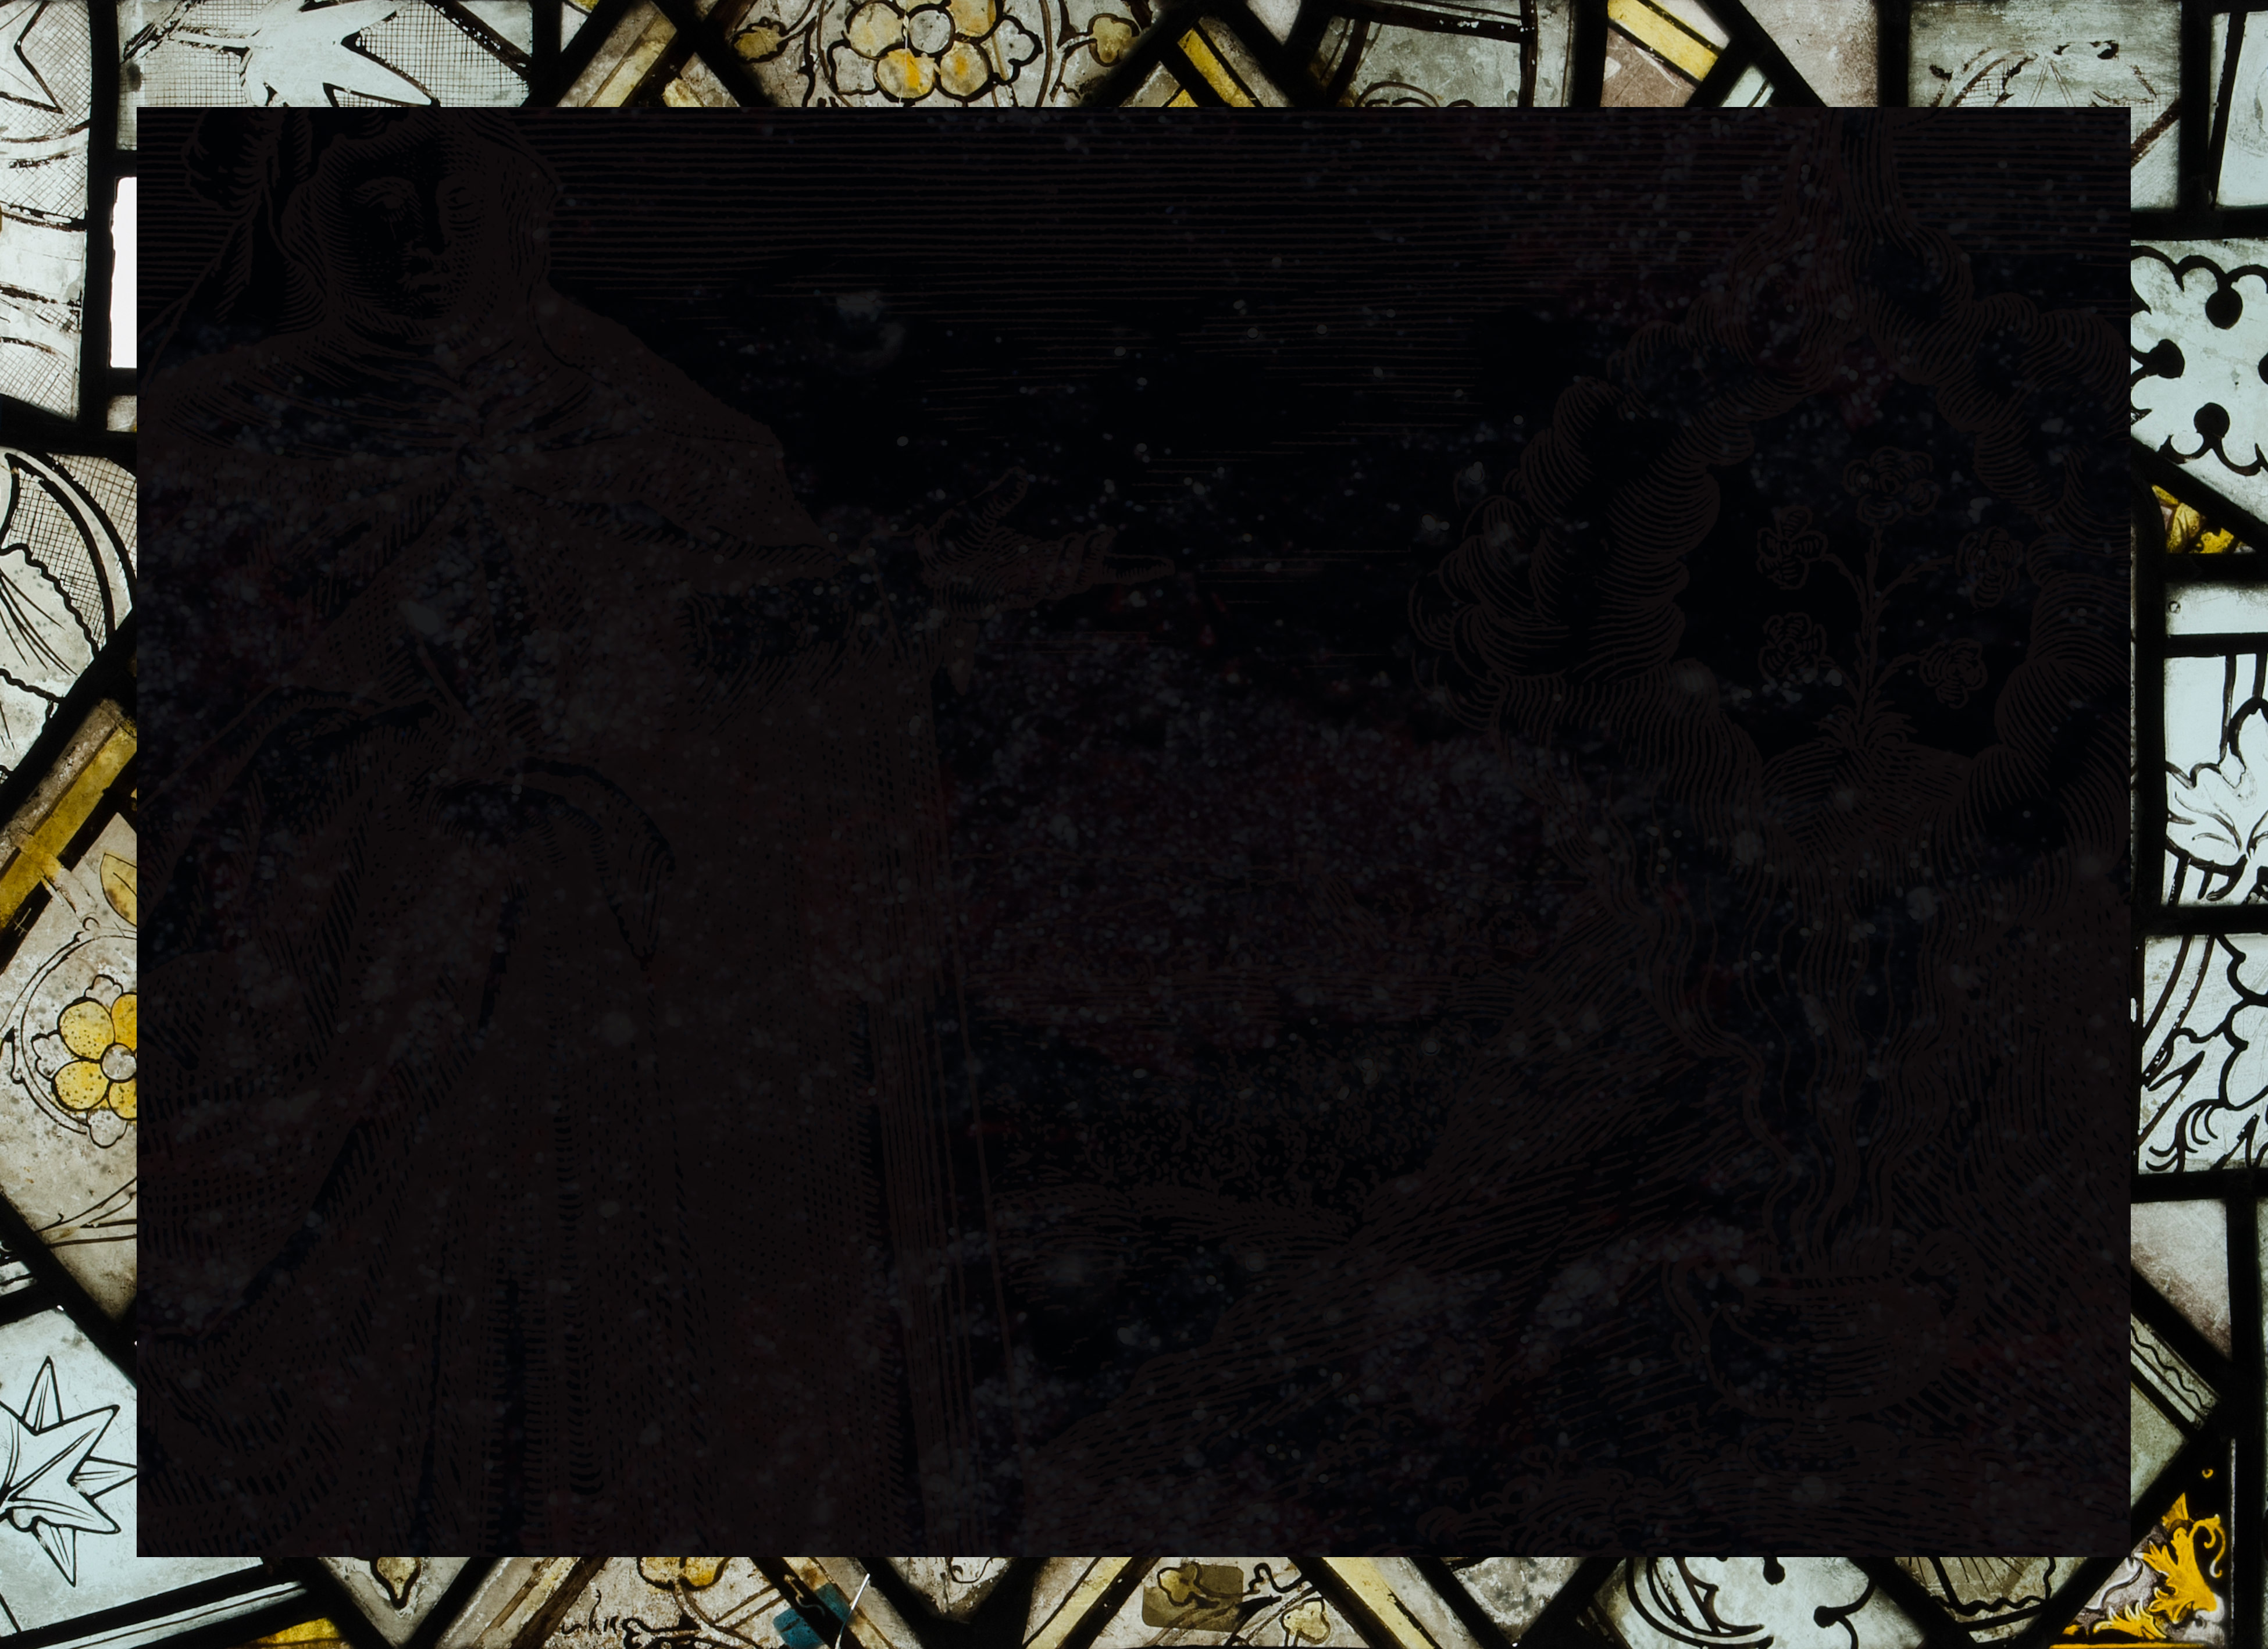
\includegraphics[width=\paperwidth,height=\paperheight]{alchemy01.jpeg}}
\begin{titlepage} % Suppresses headers and footers on the title page
	\centering % Centre everything on the title page
	%\scshape % Use small caps for all text on the title page

	%------------------------------------------------
	%	Title
	%------------------------------------------------
	
    \rule{\textwidth}{1.6pt}\vspace*{-\baselineskip}\vspace*{2pt} % Thick horizontal rule
	\rule{\textwidth}{0.4pt} % Thin horizontal rule
	
	\vspace{0.5\baselineskip} % Whitespace above the title
	
	{\scshape\Huge Collection des Anciens \\ Alchimistes Grecs}
	
	\vspace{0.5\baselineskip} % Whitespace above the title

	\rule{\textwidth}{0.4pt}\vspace*{-\baselineskip}\vspace{3.2pt} % Thin horizontal rule
	\rule{\textwidth}{1.6pt} % Thick horizontal rule
	
	\vspace{0.5\baselineskip} % Whitespace after the title block
	
	%------------------------------------------------
	%	Subtitle
	%------------------------------------------------
	
	{\scshape \normalsize Publiée sous les Auspices du Ministère de l'Instruction Publique}
	
	{\scshape Par \Large Marcellin Berthelot} % Subtitle or further description
	
	\vspace*{0.5\baselineskip} % Whitespace under the subtitle
	
        {\scshape\scriptsize Sénateur, Membre de l'Institut, Professeur au Collège de France \\Avec la Collaboration de \\\large M. Ch.-Em. Ruelle,\\\scriptsize Bibliothécaire a la Bibliothèque Sainte-Geneviève} % Subtitle or further description
  
        \vspace{\baselineskip}
  
	{\scshape \normalsize Troisième Livraison} % Subtitle or further description
  

	%------------------------------------------------
	%	Editor(s)
	%------------------------------------------------


	\vspace{\baselineskip}

	{\small\scshape Paris 1888}
	
	{\small\scshape{Georges Steinheil, Éditeur \\2, Rue Casimir-Delavigne, 2}}
	
	\vspace{0.5\baselineskip} % Whitespace after the title block

    \scshape Internet Archive Online Edition  % Publication year
	
	{\scshape\small Utilisation non commerciale --- Partage dans les mêmes conditions 4.0 International} % Publisher
\end{titlepage}
\pagestyle{fancy}
\fancyhf{}
\cfoot{\bfseries{\thepage}}
\Large
\setlength{\parskip}{1mm plus1mm minus1mm}
\clearpage
\tableofcontents
\clearpage
\section{Texte Grec.}
\subsection{Quatrième Partie. --- Les Vieux Auteurs.}
\subsubsection{4. --- 1. ΠΕΛΑΓΙΟΥ ΦΙΛΟΣΟΦΟΥ ΠΕΡΙ ΤΗΣ ΘΕΙΑΣ ΤΑΥΤΗΣ ΚΑΙ ΙΕΡΑΣ ΤΕΧΝΗΣ.}
\paragraph{}
\emph{Transcrit sur} M, f. 62 v. ;--- \emph{Collationné sur} A, f. 222 v. ;--- \emph{sur} K (copie de M ? ) f. 72 v. ;--- \emph{sur} Lc, p. 49. --- \emph{Contenu aussi dans les mss. de Vienne} (cod. med. gr., 51 et 52, \emph{dériνes de} M).

\bigskip

1. Οἱ μὲν προγενέστεροι καὶ ἐρασταὶ καὶ ἀνάπλεοι φιλόσοφοι\footnote{Réd. de A : ἀνάμπλεοι μαθημάτων καθ' ἑαυτων φιλ. ὄντες φάσκουσιν ὅτι. --- ἀν. τῶν μαθημάτων Lc.} ἔφησαν ὅτι πᾶσα τέχνη ἕνεκεν τοῦ τέλους αὐτῆς ἐπινοεῖται τῷ βίῳ · οἷον ἡ τεκτονικὴ μία οὖσα διὰ τοῦτό ἐστιν ἵνα ποιήσῃ θρόνον ἢ\footnote{μία ο. τῶν τεχνῶν Lc.} κιβωτὸν ἢ πλοῖον ἀπὸ μιᾶς φύσεως τοῦ ξυλίνου. Οὐκοῦν καὶ ἡ\footnote{ξύλου Lc.} βαφικὴ τέχνη ἕνεκεν τούτου ἐπενοήθη, ἵνα βαφήν τινα καὶ ποιότητα ποιήσῃ, ὃ καὶ τέλος τῆς τέχνης ἐστίν. Καὶ λοιπὸν χρὴ γινώσκειν (f. 63 r.) ὅτι ὀρθῶς ἀναφέρεται παρὰ τῶν ἀρχαίων λεγόντων · « ὁ χαλκὸς οὐ βάπτει, ἀλλὰ βάπτεται · καὶ ὅταν βαφῇ, βάπτει. » Διὰ τοῦτο καὶ ὁμοίως πᾶσαι αἱ γραφαὶ καματεύονται τὸν χαλκὸν,\footnote{κατακαμ. A Lc.} ἵνα βαφῇ · ἐὰν γὰρ βαφῇ, τότε βάπτει, καὶ ἐὰν οὐ βαφῆ, οὐ δύναται βάψαι, ὡς εἴρηται. Διὰ τοῦτο παρακελεύονται τὸν χαλκὸν ἄσκιον γενέσθαι,\footnote{πάντες παρακελ. Lc.} ἵνα τὴν σκιὰν αὐτοῦ ἀποβαλλόμενος δύναται δέξασθαι τὴν\footnote{δύναται] δύνατε A ; δύναιτο Lc. F. l. δύνηται.} βαφήν · σκιὰν δὲ χαλκοῦ νόησον, τὴν παρ' αὐτοῦ ἐνγινομένην ἐν τῷ\footnote{Lignes verticales, en guise de guillemets, alternativement sur les marges intérieure et extérieure de Lc, jusqu'à la fin de notre § 3.} ἀργύρῳ μελανίαν · οἶδας γὰρ ὅτι ὁ χαλκὸς οἰκονομηθεὶς καὶ ἐπιβληθεὶς\footnote{ἐν τῶ s. de l'argent puis καὶ τοῦ ὕδατος ἡ μελανία A ; ἐν τῷ ἀργύρω (en toutes lettres) καὶ τῷ ὕδατι Lc.} τῷ ἀργύρῳ μελανοῖ αὐτὸν ἔξωθεν καὶ ἔσωθεν.\footnote{Réd. de Lc : καὶ πάντες αὐτὴντὴν μελ.} Ταύτην οὖν τὴν μελάνωσιν τὴν γενομένην ἐν τῷ ἀργύρῳ σκιὰν αἱ γραφαὶ λέγουσιν · καὶ τούτου ἕνεκεν δεῖ οἰκονομεῖσθαι τὸν χαλκὸν, ἕως μηκέτι δύναται ποιεῖν μελανίαν, ἐπιβαλλόμενος ἐν τῷ ἀργύρῳ.

2. Οὕτως δεῖ οἰκονομεῖσθαι τὸν χαλκὸν, ἤγουν τὸν φυσικὸν χρυσὸν, ἕως ἂν μηδεμίαν μελάνωσιν ἐμποιῇ ἐν τῷ ἀργύρῳ · διὰ τοῦτο γὰρ καὶ Δημόκριτος ἔλεγεν · « Δοκίμαζε τὸν χαλκὸν εἰ γέγονεν\footnote{Cp. p. 46, l. 1.} ἄσκιος · ἐὰν γὰρ μὴ γένηται ὁ χαλκὸς ἄσκιος, μὴ μέμψῃ τὸν χαλκὸν, ἀλλὰ σεαυτὸν μέμψαι.\footnote{Après μέμψαι] ἐπεὶ μὴ καλῶς ᾠκονομήσας Lc (d'après A).} »

3. Οἰκονομεῖται δ' ὁ χαλκὸς διὰ τοῦ θείου ὕδατος ζυμούμενος καὶ λειούμενος καὶ ὀπτώμενος καὶ πλυνόμενος. » Πλύνεται δὲ, φησὶν, ἕως ὅλως ὁ ἰὸς αὐτοῦ ἐξέλθῃ. Καὶ ἔνθεν μνήσθητι τῶν φιλοσόφων εἰπόντων\footnote{ὅλος ὁ ἰὸς Lc.} · « Μετὰ τὴν τοῦ χαλκοῦ ἐξίωσιν καὶ μελάνωσιν καὶ ἐς ὕστερον λεύκωσιν,\footnote{ἴωσιν καὶ ἐξίωσιν Lc.} τότε ἔσται βεβαία ξάνθωσις · ἓξ ἐπιβολὰς γινομένας νόησον.\footnote{ἓξ ἐπιβολὰς] ἐξ ὑποβολῆς γινομένη · νοήσον A Lc. F. l. ἓξ μεταβολὰς. Cp. l. 22. --- A mg. Une main.} Γίνεται οὖν ἴωσις εἰς τοῦ θείου ὕδατος · ἐξίωσις δὲ, ἐν τῇ ἀποπλύσει · μελάνωσις δὲ, ὅταν πρὸ τῆς ἀποπλύσεως ὁ χρυσόλιθος μιγῇ · ἐξίσχνωσις δὲ, ὅταν ἐν τῷ χρυσολίθῳ λειωθῇ · λεύκωσις δὲ, ὅταν μετὰ\footnote{μετὰ τὴν τοῦ κουφ. ἀν. ἀναξηρανθῇ Lc.} τοῦ κουφολίθου ἀναλείωσιν ξηραίνεται · ξάνθωσις δὲ γίνεται ὅταν\footnote{ἀναλείωσιν] ἀνα puis le signe figurant l'idée de τρίψις ou de λείωσις MK. --- κωφολίθου MK.} τὰ δυνάμενα ξανθῶσαι προσπλακῇ καὶ (f. 63 v.) τοῖς μικροῖς βολβίτοις ἐντεθῇ · αὗται αἱ ἓξ μεταβολαὶ γίνονται ἐν τῷ χαλκῷ, ἵνα βαφῇ\footnote{αὗται γὰρ A Lc.} · καὶ ἐὰν μὴ γένωνται πᾶσαι, οὐδὲν γίνεται · ὡς ἐὰν μὴ γίνηται ὁ\footnote{καὶ ἕως ἂν Lc. --- πᾶσαι οὐδὲν --- μὴ γίνηται om. A ; hab. Lc.} χαλκὸς ἄσκιος ξανθὸς, οὐδὲν γίνεται.

4. Πρῶτον οὖν βάπτει καὶ μεταβάλλει καὶ κόπτει τὸν χαλκόν\footnote{F. l. βάπτε ... μετάβαλλε τ ... κόπτε et ποιεῖς.} · καὶ οὕτως διὰ τοῦ θείου ὕδατος ποιεῖ τελείαν ἴωσιν. Τελείαν ἴωσιν\footnote{ποιῆ MK.} νόησον τὴν ἐν τῇ ζύμῃ χρύσωσιν · ταύτην γὰρ καὶ αἰνιττόμενος ὁ\footnote{τὴν ἐν τῇ σήψει καὶ ζύμῃ χρ. Lc.} ἀρχαῖος ἔλεγεν · « Οἷον χρυσὸν ὁ ποιῶν ποιεῖ · ὁ δὲ μὴ ποιῶν, οὐδὲν ποιεῖ.\footnote{ὁ ἀρχ. φιλόσοφος Lc. --- ὁ ποιῶν ἰὸν χρ. π. Lc.} Ὅταν ἴδῃς τὴν τελείαν χρύσωσιν ἐν τῷ θείῳ τότε νόησον\footnote{ὅταν δὲ A Lc. ---νόησον ὅτι A Lc.} τελείαν ἴωσιν πεποίηκας, οὐ μόνον κατὰ τὴν ἐπιφανείαν τοῦ θείου ἐξανθοῦσαν, ἀλλὰ καὶ ἐν τῷ βάθει. » Σημείωσις οὖν ἐστιν ἀρχομένης\footnote{οὐ μόνον γὰρ ἐξάνθωσεν Lc.} ἰώσεως · ἡ δὲ ἐντὸς γενομένη ἴωσις αὕτη ἐστιν ἡ ἀληθινὴ ἴωσις, ἥτις καὶ ἰὸς χρυσοῦ διηρμηνεύθη · ἐὰν < δὲ > μὴ αὕτη ἴωσις γένηται, οὐδὲν γίνεται. Σκόπει οὖν ἵνα ἐν τῷ βάθει γένηται · εἰ δὲ μή γε, οὐδὲν\footnote{εἰ] ἡ M. --- Réd. de Lc : ἐὰν δὲ μὴ γίνηται ἰώσις, ἥτις καὶ ἰὸς χρυσοῦ καὶ ξανθ. εἴρ. οὐδὲν γίνεται. Διὸ καὶ ὁ φιλόσοφος ἔλεγε.} γίνεται ἴωσις, ἥτις καὶ ξάνθωσις εἴρηται μάλιστα τῷ φιλοσόφῳ λέγοντι · « Λαβὼν πυρίτην, οἰκονόμει ἕως ξανθὸς γένηται, » πυρίτην καλῶν τὸν χαλκὸν διὰ τὸ ἔμπυρον τῆς φύσεως · ὅτι οὕτω δεῖ γενέσθαι\footnote{καλεῖ A Lc. --- οὕτω δὲ δεῖ Lc.} αὐτὸν, ἵνα τελεία ἴωσις γένηται.

5. Καὶ οὕτως μέτελθε ἐπὶ τὴν ἐξίωσιν, σημειούμενος κἀνταῦθα πάλιν,\footnote{καὶ οὕτως μέτελθε] μετὰ δὲ ταῦτα, ἔρχου Lc.} « ἕως οὗ γένηται ἐξίωσις. » Ἔσται πρῶτον ἡ μελάνωσις, καὶ τότε παρακολουθήσει ἡ ἐξίωσις. Λαβὼν τοίνυν χρυσόλιθον μέρος ἓν, μαγνησίαν μέρη γʹ, λείωσον χωρὶς παντὸς ὑγροῦ · λείωσον δὲ ἕως\footnote{Le signe du cinabre au-dessus de μαγνησίαν M ; καὶ μαγνησίας καὶ κινναβάρεως Lc.} περιπλακῶσιν ἄλληλα καὶ συμμιγῶσιν αἱ οὐσίαι. Καὶ μηκέτι τοῦ θείου\footnote{μηκέτι] μὴ τὶ (l. μή τι) A Lc. --- φαίνηται Lc.} τοῦ λευκοῦ φαίνεται · γίνεται δὲ πάνυ μέλαν ὡς τὸ γραφικὸν μέλαν. Τοῦτο ἔασον ἡμέρας γʹ, καὶ βαλὼν τότε ἐν τῷ κολύμβῳ, ἐπίβαλλε τοῦ\footnote{Réd. de A Lc : ἐπίβαλλε τὸν ζωμὸν τοῦ ἰωθέντος, καὶ ἀναλύων, καὶ τρίβων, καὶ πλύνων, καὶ ἀποπλύνων, ὄψει τὸ θεῖον περιτρέχον.} ζωμοῦ τοῦ εἰωθότος πλύνειν, καὶ ἀναλείου, καὶ ἀπόπλυνον, καὶ ὄψει τοῦ θείου περιτρέχοντος. Καὶ πῶς (f. 64 r.) οἰκονομεῖται ; καὶ πῶς ἄκαυστον\footnote{Réd. de Lc (d'après A corrigé) : καὶ πῶς ἄκ. ἔ. φ. καὶ πῶς ἔχει τὸν χαλκὸν πυρίτην ; πυρίτην δὲ καλεῖ τὸν μόλ. τοῦ θείου · ἀποπλύνον δὲ, φησὶ, τὸν χαλκὸν, ἕως οὗ ὁ ἰός α. ἐ.} ἔχει φύσιν ; τὸν χαλκὸν πυρίτην καλῶν τὴν μόλιβδον τοῦ θείου\footnote{F. l. χαλκοπυρίτην.} ἀπύρου · ἐτήσιον δὲ τὸν χρυσολίθον ἀπόπλυνον, ἕως οὗ, φησὶν, ὁ ἰὸς αὐτοῦ ἐξέλθῃ. Καὶ οὕτως ἀπέρχεται μηδὲν, τοῦ χαλκοῦ ἀπομένοντος\footnote{ὑπομένοντος A Lc.} ἐν τῇ μολίβδῳ. Αὕτη μεγάλη κάθαρσις καλεῖται · αὕτη ὁμοῦ καλεῖται ἐξίωσις καὶ μελάνωσις · μελάνωσις δὲ διὰ τὸ μελαινόμενον τῆς κράσεως, ἐξίωσις δὲ, διὰ τὴν ἀπὸ τοῦ ἰοῦ ἔξοδον καὶ ἀπόλυσιν,\footnote{καὶ ἀπόλουσιν A ; om. Lc.} ἣν καὶ ἀπόπλυσιν λέγουσιν. Ταύτην οὖν δεξάμενος ἐν ἄγγεσιν,\footnote{ἣν καὶ ἀπόλουσιν καὶ ἀπόπλυνσιν A Lc. --- ταύτην] ταῦτα A Lc.} ἔα καταστῆναι. Καί ἀφυλίσας τοῦ ζωμοῦ, ξήρανον τὴν ὑποστάθμην,\footnote{τὸν ζωμὸν Lc.} ταύτην εὑρήσεις ὡς γραφικὸν μέλαν. Τοῦτο τρίβε ἕως οὗ γένηται ξανθὸν τέλειον. Τοῦτο ἐπίστρεψον καὶ ἐπίχεε ἐκ τῆς ῥητῆς μέρη\footnote{ἐπίστρεψον] ἐπίρριψον A Lc. --- ῥητῆς] ῥυτῆς Lc. Cp. 3, 6, 2 et 7, 5.} δʹ, τῆς ξανθῆς μέρος αʹ, τῆς μολίβδου μέρος αʹ · καὶ νοτίασον μικρὸν,\footnote{τῆς μολ. μ. αʹ om. A ; hab. Lc. --- νοτίασον] ἀνάδευσον A Lc. F. l. νότισον.} ἕως γένηται πηλός · καὶ λείωσον ἕως ἀφαντωθῇ ἡ μόλιβδος. Καὶ κούφισον καὶ ὡς πηλὸν ἀπόθου ἐν ἡλίῳ · καὶ ἔα ξηραίνεσθαι, ποτίζων κατὰ μικρὸν, ἕως οὗ ἡ μόλιβδος ἀναλωθῇ, καὶ ἔα ξηρανθῆναι\footnote{καταμικρὸν M.} · ἔνθεν ἐπιβαλοῦ θεωρίαν.\footnote{ἐπιβάλλει A Lc.}

6. Ὁ δὲ ἀρχαῖος Ζώσιμος ἔλεγεν. Μίαν τάξιν οἶδα ἐγὼ, δύο δὲ ἔργα ἔχουσαν · μίαν μὲν, ἵνα ῥεύσῃ διὰ τῆς ῥητῆς, καὶ δεύτερον,\footnote{ῥυτῆς Lc. Cp. 3, 7, 5. --- δευτέρα A ; δευτέραν δὲ Lc.} ἵνα ξηρανθῇ ἡ ὑγρότης τῆς μολύβδου. Οὕτω καὶ νῦν ποίησον,\footnote{τοῦ μολ. εἰς κένωσιν · (εἰς ἀκένοσιν A) καὶ οὕτως ἐπιβ. A Lc.} ξηραίνων · καὶ οὕτως ἐπίβαλλε τοῦ κουφολίθου τὸ ἶσον, καὶ λείωσον\footnote{κωφολίθου MK ici et plus loin.} ὄξει τῷ διὰ τοῦ γερανίου, ἕως ἂν λευκανθῇ · ἕως οὗ γένηται λευκὸν.\footnote{ἕως οὗ ... ] ἤγουν ἕως γέν. λ. A ; ἤγουν ἕως οὗ ... Lc. --- ἕως οὗ γ. λ.] Glose marginale insérée dans le texte ?} Βλέπε οὖν μὴ ἀκηδιάσῃς ἐν τῷ καιρῷ τῆς λευκώσεως · ἀκηδία γὰρ\footnote{Βλέπε ... ] Cp. 3, 6, 20. --- γὰρ] δὲ A Lc.} γίνεται διὰ τὸ μὴ βλέπειν τὸ κάλλος ἐκεῖνο, ὅτι διὰ τῆς λευκώσεως\footnote{ἐπιβλέπειν A Lc.} ταύτης ἄσκιος ὁ χαλκὸς γίνεται, ἀποβαλὼν πᾶσαν τὴν αὐτοῦ γεώδη ὑπερουσίαν καὶ παχύτητα τοῦ σώματος. Ἐὰν οὖν λευκανθῇ ὁ χαλκὸς ἄσκιος, πνευματικὸς γίνεται, καὶ λοιπὸν οὐδὲν ἄλλο λείπει, οὐδὲν ὑστερεῖ · εἰ μὴ μόνον ἵνα ξηρανθῇ καὶ λευκανθῇ. Ὧδε νόησον · πάντα\footnote{εἰ μὴ μόνον --- μένει (l. suiv.) om. A, hab. Lc. --- νόησον ὅτι π. τὰ χ. Lc.} χεόμενα πάν- (f. 64 v.) τα ἀποβάλλει · καὶ οὐδὲν μένει, εἰ μὴ ὁ χρυσὸς καὶ ὁ μόλυβδος καὶ ὁ ἐτήσιος λίθος ὃ καλεῖται χρυσόλιθος.\footnote{ὃς καλ. Lc. --- Le signe du cinabre sur χρυσολ. M ; à la suite A.} Γλυκάνας οὖν τὸ ξηρίον, καὶ ξηράνας, στῆσον καὶ ἐξίσασον τὸ ξηρίον τοῦ χαλκάνθου μέρη γʹ, μαγνησίας μέρος αʹ, χαλκοῦ μέρος αʹ, ἐξίσου\footnote{ἐξίσου] ἐξίωσον A ; om. Lc.} τὸ ξηρίον μέρος αʹ · λείωσον ὁμοῦ ποτίζων ἐν ἡλίῳ ἀπὸ τοῦ ὄξους τοῦ λευκοῦ ἡμέρας ζʹ · καὶ ὕστερον ξηράνας, κατάθου ἐν βολβίτοις, καὶ ἔασον ὀπτᾶσθαι ἡμέρας δύο ἢ τρεῖς, καὶ ἐξενέγκας, εὑρήσεις βαφέντα τὸν χρυσὸν, πυρρὸν ὡς τὸ αἷμα. Αὕτη ἐστὶν κιννάβαρις\footnote{πυρὸν MAK.} τῶν φιλοσόφων καὶ χαλκὸς ἄσκιος ξανθός. Ὧδε μνήσθητι ὡς ἔλεγεν\footnote{ὡς ἔλ. ὁ ἀρχαῖος] τί ἔλ. ὁ ἀ. φιλόσοφος ; Lc.} ὁ ἀρχαῖος · « Ὁ χαλκὸς ἄσκιος γενόμενος πᾶν σῶμα βάπτει. » Διὰ τοῦτο\footnote{Réd. de Lc : διὸ καὶ παρακατιὼν ἔλεγεν ὁ αὐτός.} καὶ ὁ φιλόσοφος εἶπεν · « Τί ὑμῖν καὶ τῇ πολλῇ ὕλῃ, ἑνὸς ὄντος τοῦ φυσικοῦ, καὶ μιᾶς φύσεως νικώσης τὸ πᾶν ; » Νοῶμεν ὃτι « φυσικοῦ\footnote{τοῦ φυσ. λέγει, ἤγουν τοῦ κ. φ. χρ. A Lc.} » λέγει τοῦ κατὰ φύσιν χρυσοῦ · οὗτος γὰρ ὁ κατὰ φύσιν χρυσὸς νικᾷ τὸ πᾶν τῶν ὑποκειμένων σωμάτων, οἷον ἀλειφόμενος κατὰ σίδηρον ἢ χαλκὸν νικᾷ τὴν ἐπιφάνειαν αὐτῶν καταφαινόμενος τὸν\footnote{νικᾷ ... ] Réd. de A Lc : νικᾷ τὴν φύσιν φαίνων αὐτὸν signe de l'or. --- φαίνι (l. φαίνοι) ἂν A.} κατα φύσιν χρυσόν.

8. Οὕτως οὖν διαλυόμενος διὰ τοῦ θείου ὕδατος, ζυμούμενος ὡς ἡ\footnote{διαλειούμενος A Lc. --- καὶ ζυμ. Lc.} ζύμη τοῦ ἄρτου, εἶτα καὶ τοῦ χρυσολίθου ἐξίσου συνλειουμένου\footnote{Le s. du cinabre sur χρυσολ. M. --- Réd. de Lc : Τοῦ χρυσολ. καταλαμβανομένου καὶ ἐξ ἴσου συλλ., καὶ τοῦ ὕδ. ἀπολλυμένου κατὰ τὴν φύσιν αὐτοῦ.} · καὶ τοῦ μὲν ὕδατος ἀπολυομένου κατὰ φύσιν αὐτοῦ διὰ τῆς ῥεύσεως,\footnote{ἀπολειωμένου A. --- καταφύσιν MK ici et plus loin.} καὶ τοῦ χρυσολίθου λαμβανομένου μετὰ τῆς ἐπιπλοκῆς τοῦ φυσικοῦ.\footnote{καταλαμβ. Lc. --- Le s. de l'or sur φυσικοῦ M. --- Après ce mot Lc aj. τὸ μυστήριον οἰκονομεῖται.} Ζώσιμος · « Ὁ φυσικὸς χρυσὸς πνεύματος γενόμενος διὰ τοὺ χρυσολίθου\footnote{Ὁ Ζώσ. δέ φησιν Lc. --- ὁ φυσικὸς om. A Lc. --- πνς M ; πνικὸς A Lc, f. mel.} κατὰ φύσιν βάπτει. » Καὶ ὅτι καὶ ὁ ἄργυρος, ἐὰν διαλύσωμεν\footnote{βάπτεται A.} διὰ τοῦ θείου ὕδατος καὶ πνευματικῶς ποιήσωμεν διὰ τοῦ χρυσολίθου,\footnote{πνικὸν A Lc, f. mel.} βάπτει τὸν χαλκὸν λευκὸν · τοῦτο γὰρ καὶ δι' ἑτέρων ἔλεγεν · αἱ γὰρ δύο βαφαὶ οὐδενὶ διαφέρουσιν ἀλλήλων, ἀλλὰ χρώματι μόνον, τουτέστι\footnote{Réd. de Lc : τουτέστι καταβαφῇ · καὶ γὰρ τὰ δύο σώματα διὰ τ. θ. ὕ. τὸ πρῶτον ... γενόμενα διαφ. τῷ χρ. μόνον.} μίαν μὲν καὶ τὴν αὐτὴν ἔχοντα οἰκονομίαν, ἐφ' ἧς καὶ διὰ τοῦ θείου ὕδατος πρῶτον λειούμενα, ὕστερον δὲ διὰ τοῦ χρυσολίθου πνευματικὸν ξηρίον γενό- (f. 65 r.) μενον · διαφέρουσι δὲ τῷ χρώματι, ὅτι ἕκαστον αὐτῶν κατὰ τὴν ἰδίαν φύσιν βάπτει · ὁ μὲν χρυσὸς, χρυσὸν, ὁ δὲ ἄργυρος\footnote{ὁ μὲν χρυσὸς --- θερίζει (l. 10) om. A Lc.} τὸν ἄργυρον. Οὐκ ἀκούεις τὸν ἀρχαιότατον λέγοντα · « Ὁ σπείρων σῖτον,\footnote{F. l. τῶν ἀρχαιοτάτων λεγόντων. --- Cp. 1, 13, 8 ; 13 bis, 6 ; 3, 16, 6.} σῖτον γεννᾷ καὶ θερίζει, καὶ ὁ χρυσὸς χρυσὸν γεννᾷ · ὁμοίως καὶ ἄργυρος ἄργυρον γεννᾷ. »

9. Διὰ τοῦτο καὶ ὧδε ὁ ἀρχαῖος ἔλεγεν · « Χρησόμεθα τοῖς φυσίκοῖς.\footnote{ὁ ἀρχ. φιλόσοφος ἐβόα λέγων Lc.} » Ἔστι δὲ ἀναγκαῖον εἰδέναι ὅτι ὁ μὲν χρυσὸς φυσικῶς βάπτει,\footnote{δὲ] F. l. γὰρ. --- χρησύμ., χρησόμεθα A ; χρησώμεθα, χρυσώμετα Lc. --- Réd. de Lc : ὁ μὲν φυσικὸς χρυσὸς βάπτει · ὁ δὲ μὴ φυσικὸς οὐ βάπτει, χωρὶς ...} οὐ χωρὶς τοῦ πρότερον διαλυθῆναι αὐτὸν διὰ τοῦ θείου ὕδατος, καὶ ὕστερον πνευματωθῆναι διὰ τοῦ χρυσολίθου · κατὰ φύσιν γὰρ καὶ\footnote{γὰρ] δὲ A Lc.} στερεὸν σῶμα καλούμενος · δεῖ τε πρῶτον διαλυθῆναι, καὶ ὕστερον\footnote{δεῖται Lc, f. mel.} πνευματωθῆναι · καὶ οὕτως παντὸς φυσικοῦ βάπτει. Τὰ γὰρ ἄλλα\footnote{F. l. πάντα φυσικῶς βάπτει.} δύο κατὰ τὴν ἰδίαν φύσιν φευκτὰ καὶ καυστὰ ἐν τῷ πυρὶ ἀναλίσκονται · ὅθεν ὁ ἀρχαῖος Ζώσιμος ἔλεγεν · « Ὅτι γὰρ αὐτὸ τὸ\footnote{Réd. de A : ὅθεν ὁ ἀ. Ζ. ἔλεγεν · ἀλλὰ καὶ αὐτὸ τὸ ξηρίον ποτιζώμενον (\emph{sic}) δυνάμενον ἀποστύφειν ἐν τοῖς ζωμοῖς, ἵνα ἐν τῆ σύψη (l. σήψει) βαφῆ ἐν τοῖς ζωμοῖς, καὶ αὐτὸ τὸ μυστήριον ... Réd. de Lc : ὅθεν καὶ ὁ ἀ. Ζ. ἔλεγεν ὅτι καὶ αὐτοῦ τοῦ μυστηρίου τοῦ τῆς καταβαφῆς τὰ σώματα γίνονται πνεύματα.} μυστήριον τὸ τῆς χρυσοβαφῆς · σώματα ὄντα πνεῦμα γίνεται, ἵνα ἐν\footnote{πνεύματα A.} ταῖς καταγραφαῖς πνευματικῶς βάψῃ, καὶ μὴ ἐπενέγκῃ ἐπισταθμίαν\footnote{καταγραφαῖς πνευματικῶς] καταβαφαῖς τοῦ πνεύματος A Lc. --- βάψωσι Lc. --- ἐπὶ σταθμίαν M. --- M. mg. : ὦ κα (lire ὧ καλόν ! ).} · στερεὰ γὰρ ὄντα, βάπτειν οὐ δύνανται, ἐὰν μὴ πρῶτον λεπτυνθῇ καὶ\footnote{λεπτυνθῇ καὶ πνευματωθῇ] Le pluriel dans Lc.} πνευματωθῇ. Λεπτύνει μὲν αὐτὰ πρῶτον τὸ θεῖον ὕδωρ · πνευματοῖ δὲ ὕστερον ὁ χρυσόλιθος. Οὐκοῦν σημειωσώμεθα ὅτι, δύο βαφῶν ὄντων\footnote{ὄντων] οὐσῶν Lc.} κατὰ τὴν τῶν δύο σωμάτων ἰδίοτητα, τὰ ἄλλα ὡς μεσιτεύουσι\footnote{ὡς μεσιτεύοντα μεταλαμβάνουσι τ. β. καὶ μεταδιδοῦσιν Lc.} μεταλαμβάνοντα τὴν βαφὴν καὶ μεταδιδοῦντα · μεταλαμβάνοντα μὲν, τὰ διαλύοντα καὶ πνευματοῦντα, μεταδιδοῦντα δὲ, τὰ χεόμενα αὐτὴν\footnote{μεταδιδοῦσι δὲ τοῖς χεομένοις διὰ τοῦ χων. Lc.} διὰ τοῦ χωνευτηρίου. Καὶ χρὴ λοιπὸν σημειώσασθαι ὅτι, ὥσπερ\footnote{Καὶ χρ. λ. σημ.] Διὸ χρὴ σημ. Lc.} ἀλειφόμενος χρυσὸς, ἢ ἄργυρος, ἢ σίδηρος, ἢ χαλκὸς οὐ κρατεῖ, ἐὰν μὴ τοῖς ζωμοῖς προστυφθῇ οὕτως οὔτε νῦν ὧδε κρατεῖ, οὔτε χρυσὸς, οὔτε ἄργυρος, ἐὰν μὴ προστυφθῇ, ἀλλὰ καὶ αὐτὸ τὸ ξηρίον ποτίζειν\footnote{ποτίζειν δυν. οὐδὲν ἔσται ἐὰν μὴ τοῖς ζωμοῖς ἀποστ. ἵνα ... Lc.} δυνάμενον ἀποστυφθῇ ἐν ζωμῷ, ἵνα τὴν στύψιν ἡ βαφὴ εἰσ- (f. 65 v.) κρίνουσα\footnote{ἐν ἡλίω (en toutes lettres ; lire χρυσῷ ? ) εἰσκρίν. A.} καὶ διαδύνασα εἰς βάθος, στύψῃ καὶ κρατήσῃ ἐκεῖ κατὰ\footnote{διαδύνουσα A Lc. --- στύψει καὶ κρατήσει MK.} βάθος τοῦ σώματος, διαλυομένου τοῦ ξηρίου. Διὰ τοῦτο ἡ φύσις\footnote{καταβάθους MK. --- διαλειωμένου A Lc (Lc a eu διαλυομένου). --- ἡ φύσις τὴν φύσιν κρατεῖ καὶ τέρπει A Lc.} τῇ φύσει τέρπεται. » Καὶ τὰ ἑξῆς.

10. Νόησον γὰρ ταῦτα καὶ ἐπὶ τοῦ σώματος λαμβανόμενα,\footnote{Ταῦτα δὲ πάντα νόησον Lc. --- λαμβάνεσθαι Lc.} καὶ ἐπὶ τοῦ θείου ὕδατος, καὶ ἐπὶ τοῦ χρυσολίθου, καὶ ἐπὶ τῶν στυφόντων ζωμῶν. Ἆρα γὰρ οὐ χαίρει ἡ φύσις τοῦ σώματος ; χαίρει τῇ φύσει\footnote{τῷ σώματι Lc. --- χαίρει δὲ τῇ φ. Lc.} τοῦ ὕδατος τρεφομένη καὶ παχυνομένη καὶ αὐξανομένη. Ἆρα οὐ τέρπεται καὶ λαμπρύνεται ὁ χαλκὸς, ἀτερπὴς καὶ ἀλαμπὴς ὢν τῇ οὐσίᾳ τῆς τερπνῆς καὶ λαμπροτάτης τοῦ θείου ὕδατος φύσεως ; Ἆρα οὐ νικᾶται ἡ φύσις τοῦ παχυτέρου καὶ γεωδεστέρου σώματος ὑπὸ τῆς φύσεως τοῦ χρυσολίθου, πνευματικῆς καὶ ἀερώδους οὔσης\footnote{φύσεως --- γεωδεστέρου om. A ; hab. Lc.} ; Ἆρα οὐ κρατεῖται τοῖς στύφουσι ζωμοῖς ὡς ἀλειφόμενος χρυσὸς καὶ ἄργυρος ἐν σιδήρῳ ἢ χαλκῷ ; Ταῦτα πᾶσι κοινῶς δεῖ ὁμολογεῖν ὅτι,\footnote{Réd. de Lc : Ταῦτα κοινῶς πάντας ὁμολ. δεῖ.} εἰ μὴ στυφθῇ σίδηρος ἢ χαλκὸς ἀλειφόμενος, χρυσὸς ἢ ἄργυρος οὐ\footnote{Réd. de Lc : ὁ σίδ. ἀλ. ἢ ὁ χαλκὸς χρυσῷ ἢ ἀργύρῳ ... --- Réd. de Lc : οὐ κρ. ἡ φύσις, τουτέστιν οὐ νικᾶται --- σώματος (comme plus haut) ; variante analogue dans A.} κρατεῖ, ἐπειδ' ἂν δὲ στυφθῇ, τότε ἀλειφθῇ, τότε κρατεῖ δυνάμει τοῦ\footnote{δὲ om. A ; hab. Lc. --- τότε ἀλ.] καὶ ἀλ. Lc. --- δυνάμει] ἡ δύναμις Lc.} στύφοντος.\footnote{κινναβάρεως (en signe) τοῦ στύφ. A.}

11. Ἀλλ' ἐρεῖ τις πρὸς αὐτὸν ταῦτα · εἰ χρυσὸς ἢ ἄργυρος ὡς\footnote{πρὸς αὐτὸν] πρὸς ἡμᾶς Lc. --- ὁ χρ. ἢ ὁ ἄργ. τῶν δ. β. ὄντα ποιητ. καὶ ποιοῦσι ξηρία Lc.} δύο βαφῶν ποιητικὰ ποιεῖται ξηρία, πῶς παρακολουθήσει ἴωσις καὶ ἐξίωσις καὶ ἐξίσχνωσις καὶ μελάνωσις, εἶθ' οὕτως ὕστερον λεύκωσις ; Τότε ἔσται βεβαία ξάνθωσις κατὰ τὰ προδιαγραφέντα. Καὶ λέγομεν ὅτι πάντα παρακολουθεῖ δυνάμει κατὰ ἀμφοτέρων ταῖς βαφαῖς. Ἐπειδὴ γὰρ εἴρηται ὅτι ἴωσις καλεῖται ἡ ἐν τῷ θείῳ ὕδατι διάλυσις,\footnote{ἐπ. --- ὅτι] εἴρηται γὰρ ὅτι Lc.} δυνάμει παρακολουθεῖ ἐν τῷ ὕδατι καὶ ἡ ἐξίωσις, καὶ ἡ ἐξίσχνωσις, καὶ ἡ μέλανσις, καὶ ἡ λεύκωσις μετὰ τὸ γενέσθαι, ὕστερον βεβαία\footnote{ὕστερον] ξηρίον A Lc, f. mel.} ξάνθωσις, οὐ μόνον δυνάμει, ἀλλὰ καὶ ἐνεργείᾳ, ἅπαντα παρακολουθεῖ πρὸ τοῦ γενέσθαι λευκὸν τὸν χρυσὸν, ὕστερον δὲ βεβαία ξάνθωσις, ἕως ὁ πνευματικὸς τέλειος ἀποτελεσθῇ καὶ συνυπακούσηται.\footnote{συναπακούσῃ Lc.} Καὶ αὖθις ὀρθῶς ἔφη λέγων ὁ φιλόσοφος · « Ὦ φύσεις οὐρανίαι φύσε- (f. 66 r.) ων\footnote{ὀρθῶς om. A. ; hab. Lc. --- Cp. Démocrite, § 14 (ci-dessus, p. 46).} δημιουργοί, » τρόπῳ γὰρ δημιουργίας αἱ δύο φύσεις τῶν θείων, κατά τε τὸ ὕγρον τῆς κράσεως, κατά τε τὸ ξηρὸν τῆς\footnote{Le signe de la magnésie sur κράσεως M ; κράσεως τῆς μαγ νησίας ALc (τῆς om. A).} οὐσίας τὰς γεώδεις φύσεις τῶν σωμάτων πνευματικὰς καὶ βαφικὰς\footnote{Le signe du cinabre sur οὐσίας M ; τῆς μαγνησίας A Lc (τῆς om. A).} ἐδημιούργησαν. Οὐράνιαι γὰρ αἱ φύσεις τῶν θείων τούτων οὐχ ἑρμηνεύονται ὡς δυνάμεναι αἱρεῖσθαι. Διὸ καὶ ἑξῆς λέγει · « Οὐδὲν ὑπολέλειπται,\footnote{αἱρεῖσθαι] αἰ ῥήσται A. Lire αἴρεσθαι. --- ὁ φιλόσοφος λέγει Lc. --- Cp. Démocrite, ci-dessus, p. 53.} οὐδὲν ὑστερεῖ, πλὴν τῆς νεφέλης καὶ τοῦ ὕδατος ἡ ἄρσις, ἀντὶ τοῦ εἰπεῖν « οὐδὲν ἄλλο ἐστὶ τὸ προσδοκώμενον, » ἔφη · « ἄλλη τὸ λικμησθῆναι τὸ σῶμα, ὡς ἡ νεφέλη τοῦ ὕδατος,\footnote{ἄλλη] ἀλλ' ἡ A ; ἀλλ' ἢ Lc. F. l. ἀλλ' εἰ.} καὶ ἀρθῆναι πάλιν τὸ ὕδωρ ἀπ' αὐτοῦ, καὶ ἰδοὺ ἐπιστοιχείου τὸ πᾶν.

12. Ἄρσις δὲ ἑρμηνεύεται ὁ κουφισμὸς, ἄνθ' ὧν αἴρεται καὶ κουφίζεται\footnote{Le texte de notre § 12 complète et rectifie celui de 3, 2, 3. --- ἀνθῶν MA.} ἡ τοῦ ὕδατος ἐπίχυσις ἐκ τῆς τοῦ σώματος συμπλοκῆς · ἐν ἐπιμνήσει δὲ ποιῆσαι ἀρκεσθῶμεν τῇ θυείᾳ καὶ τῷ δοίδυκι ἐπὶ τῶν\footnote{ἐν ἐπιμν.] ἀν' ὑπομονέστατα τούτων δεῖ π. A. Réd. de Lc : ἐν ὑπομνήσει δὲ καὶ ὑπομονῇ τοῦτο δεῖ ποιῆσαι · ἀρκεσθ. οὖν τῇ θυΐᾳ ... --- θυΐα MAK.} δύο βαφῶν · ἐπὶ δὲ τοῦ χαλκοῦ ἐπὶ τῇ χρήσει τοῦ φιαλοβωμοῦ.\footnote{τῇ χρ. --- καὶ ὅτι om. A. Cp. 3, 2, 3.} Καὶ ὅτι περὶ τούτου Ζώσιμος ἔλεγεν. Καὶ ὅτι δένδρον φυτουργούμενον,\footnote{περὶ δὲ τοῦ χαλκοῦ ὁ Ζ. ἔλ. ὅτι ...} φυτὸν ποτιζόμενον, καὶ ὑπὸ πλήθους ὕδατος σηπόμενον,\footnote{ὐδάτων AK Lc.} καὶ διὰ τῆς τοῦ ἀέρος ὑγρότητός τε καὶ θερμότητος αὐξανόμενον ἀνθοφορεῖ,\footnote{Réd. de Lc : αὐξανόμενον · ἀνθοφορεῖ δὲ ποικίλως ἀεί ποτε καὶ τῇ π. γλ.} καὶ τῇ πολλῇ γλυκύτητι καὶ τῇ ποιότητι τῆς φύσεως καρποφορεῖ.\footnote{τέλος τοῦ Πελαγίου add. Lc.}

\bigskip
\centerline{\EightStarTaper}
\centerline{\EightStarTaper\EightStarTaper}
\bigskip

\subsubsection[4. --- 2. ὈΣΤΑΝΟΥ ΦΙΛΟΣΟΦΟΥ ΠΡΟΣ ΠΕΤΑΣΙΟΝ ΠΕΡΙ ΤΗΣ ΙΕΡΑΣ ΤΑΥΤΗΣ ΚΑΙ ΘΕΙΑΣ ΤΕΧΝΗΣ.]{4. --- 2. ὈΣΤΑΝΟΥ ΦΙΛΟΣΟΦΟΥ ΠΡΟΣ ΠΕΤΑΣΙΟΝ ΠΕΡΙ ΤΗΣ ΙΕΡΑΣ ΤΑΥΤΗΣ ΚΑΙ ΘΕΙΑΣ ΤΕΧΝΗΣ.\footnote{Titre, sans nom d'auteur, dans A : περὶ τῆς θείας τέχνης : dans Lc : περὶ τοῦ θείου ὕδατος. --- ἄτρεπτον] Lambécius (Bibliotheca cæsarea, pars 2 libri 6, p. 169, pense que ce terme sert ici à désigner l'or.}}

\emph{Transcrit sur} M, f. 66 r. --- \emph{Collationné sur} A, f. 79 v. ;--- \emph{sur} K, f. 75 v. ;--- \emph{sur} Lc, p. 229. --- \emph{Contenu aussi dans} Laur., f. 88 v. \emph{et dans le ms. de Vienne dit Codex medicus gr.}, 51, f. 40 v.

\bigskip

1. Τῆς φύσεως τὸ ἄτρεπτον ἐν μικρῷ ὕδατι τέρπεται\footnote{Après ὕδατι] signe du mercure A ; τῆς ὑδραργύρου Lc.} · αἱ κράσεις\footnote{τρέπεται, τρέπουσι A Lc, mel. (\emph{M. B.}).} γὰρ αὐτὸ τέρπουσιν τῆς ὑφεστώσης ὑποστάσεως · διὰ γὰρ τοῦ ἐρασμίου καὶ θείου ὕδατος τούτου πᾶν νόσημα θεραπεύεται. Ὀφθαλμοὶ\footnote{τοῦτο τὸ νόσ. θερ. A. --- Après θεραπεύεται, Lc omet le reste de notre § 1 et tout le § 2.} βλέπουσι τυφλῶν, ὦτα ἀκούουσι κωφῶν, μογιλάλοι τρανῶς λαλοῦσιν.\footnote{μογγιλάλαις γλώσσαις (lire μογίλαλοι γλῶσσαι ? ) τρ. λαλ. A.}

2. Ἔστι δὲ εἰκότως ἡ σκευὴ τοῦ θείου ὕδατος τοιαύτη. Λαβὼν ὠὰ δρυίνου ὄφεως ἐν αὐγούστῳ μηνὶ ἐν ὄρεσι διατρίβοντος Ὀλυμπίου\footnote{ὠὰ gratté dans M, omis dans K, restitué par A. --- Signe du mercure sur ὄφεως M ; après ce mot dans A. --- Signe du cinabre sur διατριβ. M. --- Ὀλύμπου A, mel.} (f. 66 v.) ἢ Λιβάνου ἢ Ταύρου, προσφάτων ὄντων, ἔκχεον ἐν ὑελίνῳ\footnote{ἔχε A. F. l. ἔγχεε.} ἀγγείῳ λίτραν μίαν · ἐπιβαλὼν ἐν αὐτῷ ὕδατι θείῳ, ἤγουν θερμοῦ,\footnote{ἐπίβαλε εἰς αὐτὸ (l. αὐτῶ ? ) ὕδατι θερμὸν A.} ἀνάγαγε ἐν οὐρανίᾳ θεῖον ἄπυρον τετρακὶς, ἄχρις αὐτοῦ πορφυρόχροος\footnote{F. l. ἐν οὐράνῳ.} γένηται ἡ ἀνάλειψις τοῦ ἐλαίου. Λαβὼν ἀμίαντου γ° ιγʹ, αἵματος\footnote{ἀνάλιψις M ; ἀνάλυψης A. --- F. l. ἀνάληψις. --- γ° γʹ A.} κογχύλης γ° θʹ, ὠὰ χρυσοπτέρων ἱεράκων γ° εʹ, εὑρισκομένων πλησίον\footnote{ὠὰ (comme p. précéd., l. 16). --- χρυσοπτερύγων A.} τῶν κέδρων τοῦ Λιβάνου ἐν τῷ ὄρει · ταῦτα λειοτριβήσας τὰ εἴδη ἐν θυείᾳ λιθίνῃ τὴν ἀμίαντον καὶ τὴν κογχύλην καὶ τὰ ὠὰ, ἕως ἂν\footnote{τὴν ἀμ. --- τὰ ὠὰ. Ces mots semblent être une interpolation. --- ὠὰ] gratté M, laissé en blanc K, restitué par A.} ἑνωθῶσιν ὁμοῦ πάντα · καὶ μετὰ ταῦτα ἐν ὑελίνῳ ἄμβικι ἐξωράϊσον\footnote{ἄμβικι] ἄβυκη et au-dessus, en rouge ; ἀγγεῖον A (1\textsuperscript{re} main). --- ἐξοράϊσον A.} ἑπτάκις, καὶ ἀπόθες. Ἀνάγαγε τὸ πρῶτον σύνθεμα μετὰ τοῦ δευτέρου,\footnote{M mg. : ω\textsuperscript{δ} et un point en regard de cette ligne et de la suivante. --- Mα sur δευτέρου en rouge M.} καὶ λείου ἐν τρισὶν ἡμέραις · καὶ μετὰ τὴν τελείωσιν, ἐπίβαλλε\footnote{λείου] signe de λείου et de τρίψον M ; τρίψον A ; espace blanc K. Lecture conj. --- ἴωσιν sur τελείωσιν A.} ἐν ὑελίνῳ < ἀγγείῳ > πάντα ὁμοῦ λειωθέντα · καὶ θάψον ἐν ὕδατι\footnote{θάψον αὐτὸ εἰς ὕδ. νυχθήμερον αʹ A.} θαλασσίῳ ἡμέραν α` · καὶ ἐτελέσθη τὸ θεῖον ὕδωρ.\footnote{ἐτελεύθη M.}

3. Τοῦτο τὸ ὕδωρ τὰ νεκρὰ ἀνιστᾷ καὶ τὰ ζῶντα νεκροῖ,\footnote{νεκρὰ] νενεκρωμένα A. --- Sur ἀνιστᾶ, le signe Mα M ; le signe de l'or A. --- τὰ ζωντανὰ A. --- νεκροῖ] νεκρὰ M ; νεκρεῖ A.} τὰ σκοτεινὰ\footnote{Sur νεκρὰ (pour νεκροῖ), sur φωτίζει et sur σκοτίζει, le signe du cinabre M.} φωτίζει καὶ τὰ φωτεινὰ σκοτίζει, ὕδωρ θαλάσσιον δράσσεται, καὶ τὸ\footnote{ὕδωρ θαλάσσιον] τῶν puis le signe de θαλάσσιον MK ; καὶ τῶν ὑδάτων Lc. --- Réd. de A : τὸ ὕδωρ τὸ (l. τῷ) δράσαντι τὰ πάντα συνεργοῦντος τῇ τοῦ ἀοράτου καὶ παντοδυνάμου θεοῦ · δυνάμει etc.} πῦρ ἀπολύει · καὶ ταῦτα διὰ μικρᾶς σταγόνος τὰ μολιβδοειδῆ χρυσοειδῆ ἐργάζεται, συνεργοῦντος τοῦ τῇ ἀοράτῳ καὶ παντοδυνάμῳ δυνάμει\footnote{Lc omet tout ce qui suit le mot ἐργάζεται.} καὶ σοφίᾳ χρησαμένου, καὶ ἐκ μὴ ὄντος εἰς τὸ εἶναι τὰ σύμπαντα καὶ\footnote{ὄντως M.} ἀχθῆναι καὶ γενέσθαι καὶ μορφοῦσθαι κελεύσαντος · ᾧ καὶ κράτος\footnote{ἀχθ. καὶ μορφωθῆναι.} νέμειν δεῖ αὐτῷ τῷ μόνῳ, καὶ καθολικῷ καὶ ἀληθινῷ Θεῷ, σὺν τῷ ζωαρχικῷ τῆς ἡμετέρας ζωῆς καὶ σωτηρίας Χριστῷ Ἰήσου, σὺν τῷ\footnote{ὑμετίρας K.} νοερῷ καὶ ἡγεμονικῷ Θείῷ Πνεύματι, δόξα, μεγαλοπρέπεια εἰς τοὺς\footnote{θ. πν. δ. μεγαλοπρ. om. A.} ἀτελευτήτους αἰῶνας τῶν αἰώνων · ἀμήν.

\bigskip
\centerline{\EightStarTaper}
\centerline{\EightStarTaper\EightStarTaper}
\bigskip

\subsubsection[4. --- 3. ΙΩΑΝΝΟΥ ΑΡΧΙΕΡΕΩΣ ΤΟΥ ΕΝ ΕΒΕΙΓΙΑ, ΠΕΡΙ ΤΗΣ ΘΕΙΑΣ ΤΕΧΝΗΣ.]{4. --- 3. ΙΩΑΝΝΟΥ ΑΡΧΙΕΡΕΩΣ ΤΟΥ ΕΝ ΕΒΕΙΓΙΑ, ΠΕΡΙ ΤΗΣ ΘΕΙΑΣ ΤΕΧΝΗΣ.\footnote{ἐνεβειγία A ; ἐνευειγεία A\textsuperscript{2} ; ἐν Ἐβειγίᾳ K Lc.}}

\emph{Transcrit sur} A, f. 243 r. --- \emph{Collationné sur} A, f. 140 v. (= A\textsuperscript{2}) jusqu'à ἐξυδραργυρώσεως, texte biffé (ci-dessus, p. 131, l. 8) ;--- \emph{sur} Lc, page 91.

\bigskip

Nos §§ 1 à 9 sont, à part les premiers mots (Μετασκεψώμεθα καὶ ἴδωμεν ἢ φιλοσοφίσωμέν τι μᾶλλον ὁριζόμενοι, ὡς ἄρα ... ), une reproduction textuelle de la partie du traité de Zosime sur la Vertu et l'Interprétation (3, 6) comprise entre le § 15 et la fin. Nous supprimons ici ce texte dont les principales variantes ont été données dans Zosime, p. 130 et suiv.

\bigskip

10. (f. 247 r.) Ἀλλ' ἵνα δαψιλέστερα τὰ ῥεύματα ἔχοιμεν καθὰ\footnote{ῥεύματα] F. l. ῥήματα (\emph{M. B.}). --- κατὰ ἀπόῤῥοιαν Lc. --- Cp. 3, 6, 9.} ἀπορίαι τῆς σεληνιακῆς ῥεύσεως γίνονται · πορεύου κατὰ τὸ σπήλαιον\footnote{γίνωνται A ; γινέσθωσαν Lc. --- πορ. δὲ Lc.} τοῦ Ὀστάνου, καὶ ὅρα τῶν ὑδάτων τὰ ἀγγεῖα εἰς πλῆθος αὐτῷ\footnote{αὐτῷ add. Lc.} παρασκευασθέντα καὶ ποτίμου ὕδατος πληρώσας · ἢ πρὸς τὰ ῥεύματα τοῦ Νείλου πορευθεὶς, ποίησον κατὰ τὸ γεγραμμένον, ὡς προσηγόρευσεν ὁ Ἑρμῆς λέγων · « Τὸ ἀπὸ τῆς σεληνιακῆς ἀπορίας ἐκπίπτον,\footnote{ἀπορρίας A ; ἀπορροίας Lc.} ποῦ εὑρίσκεται καὶ ποῦ οἰκονομεῖται, καὶ πῶς ἄκαυστον ἔχει φύσιν, παρ' ἐμοὶ εὑρήσεις καὶ Ἀγαθοδαίμονι · τότε γὰρ ἀποριῶν τοσοῦτον\footnote{τότε --- γινόμενον] τὸ γὰρ ἀπὀῤῥέον πολὺ γενόμενον Lc.} γινόμενον εὑρίσκεται [τὸ] ἐκπεσεῖν ἐν τοῖς ὑποδεχομένοις δοχείοις, ἄκαυστον\footnote{τὸ om. Lc.} φύσιν ἔχων ξανθὴν ὡς στίγμα χρυσοῦν · τοῖς γὰρ γλυκέοις καὶ ποτίμοις\footnote{ἔχον Lc. --- Cp. 3, 6, 2 et 10.} ὕδασιν γλυκανθὲν, πᾶν τὸ ἀλλότριον ἐκφυσᾷ. Ἀνθ' ὧν καὶ εἴρηται\footnote{ἀνθῶν A. Réd. de Lc : Διὸ καὶ εἴρ. χρυσόλιθος, χρυσάνθιον, χρυσοκογχ., χρυσοζ. καὶ εἴ τινι ἄλλῳ ὀνόματι διὰ χρυσὸν κ. π. χρ. τοιούτῳ ὁ πυρ. καλεῖται.} τὸ χρυσάνθιμον, χρυσόλιθον, χρυσοκογχύλιον, χρυσοζώμιον, καὶ εἴ τι ἄλλο διὰ χρυσὸν, καὶ περὶ χρυσόν · τοιοῦτον ὄνομα ὁ πυρίτης ἐστὶν, ὅστις καλῶς λίθος λευκανθεὶς κατὰ τὸ θεῖον ὕδωρ, ἐκφυσᾶται καὶ\footnote{καλὸς Lc.} ξανθοῦται, οὕτως ἐλευθεροῦται. Καὶ ἀποξηραινόμενος ἰὸς χρυσὸς ἑρμηνεύεται\footnote{A mg. : Une main. --- ὁ ἰὸς Lc.} · ὃν καὶ ὁ ποιῶν ἰὸν ποιεῖ, ὁ δὲ μὴ ποιῶν οὐδὲν ποιεῖ.\footnote{Cp. 3, 8, 3, p. 42, l. 17.}

11. Τοῦτο ἀπέκρυψαν πᾶσαι αἱ γραφαὶ, καὶ διὰ μόνης τῆς ἐκστροφης\footnote{Ταῦτα δὲ ἀπ. Lc.} ἐδογμάτισαν, ὡς ἔλεγον · « Ἔκστρεψον αὐτοῦ τὴν φύσιν, καὶ εὑρήσεις\footnote{ἔκστρεψον ... ] Cp. 3, 29, 22.} τὸ ζητούμενον · ἡ γὰρ φύσις ἔνδον κέκρυπται, τοῦτο γὰρ φύσιν ἔχει.\footnote{τοῦτο ... ] ταύτην γὰρ τὴν φ. ἔχει Lc.} Καὶ ὅτε βούλει κα- (f. 247 v.) τεργάσασθαι, μέτελθε διὰ πάσης στηλογραφίας ἢ ὡς αὐτὸ Δημόκριτος στηλιτεύει · καὶ διάσκεψον ὅτι τὸν ἰὸν λαμβάνων, ποτὲ μὲν ἐν στυπτηρίᾳ προσπλέκει, ποτὲ δὲ ὤχραν,\footnote{εἰς ὤχ ... εἰς ἐλ. Lc.} ποτέ δὲ ἐλύδριον, ἄλλοτε ἄλλως ἐπιτηδεύων, διανοίγων τὸν νοῦν.\footnote{καὶ ἄλλοτε ἐπιτηδεύει, καὶ διανοίγει Lc.} Ὅτι δὲ αὐτὸς δύναμιν ἔχει λυτικὴν ὁ ἰὸς, ὃς βιαζόμενος ἢ λύεται ἢ εἰσκρίνει\footnote{ὃς add. Lc.} καὶ διαδύνει ἐν τῷ κινναβάρει, ἐπεὶ μηδὲν ἐπιβάλλεσθαι, διὰ τὸ [δὴ]\footnote{κινναβάρει] signe du cinabre A ; χρυσῷ Lc. --- ἐπεὶ ... ] διὸ μηδὲν ἐπιβ. δεῖ Lc. --- τὸ δὴ] δὴ om. Lc. F. l. τοδὶ.} πνεῦμα γίνεσθαι · καὶ ἐντεῦθεν τῆς σφοδρότητος τοῦ πυρὸς ἀποστρέφεται,\footnote{ἀποστρέφεσθαι, μὴ φθάνον Lc.} μὴ φθάνων εἰς βάθος τῆς καρδίας τοῦ χωνευμένου σώματος. Καὶ ἵνα ὡς διὰ μιᾶς στήλης ἔχοιμεν τὴν ὑπόμνησιν, οὕτως διασκεπτέον ὑπὲρ\footnote{ἔχομεν Lc, f. mel. --- ὑπὲρ φύσιν] F. l. εἴπερ φησὶν. --- διασκεπταίων A ; διασκεψώμεθα ὡς φιλόσοφός φησι Lc.} φύσιν. Λαβὼν ῥᾶ ποντικὸν, λείωσον οἴνῳ ἀμιναίῳ σκληρῳ, καὶ ποίησον\footnote{ἀμινέω A ; ἀμυνέῳ Lc. --- Réd. de Lc : καὶ ποίησον πάχος κηρωτῆς ὀνυχόπαχον, ἢ καὶ ὀνύχων ἰσχνότερον, καὶ χρίσον τὸ ἥμισυ τῶν πετάλων τῶν ἐξ ἀργύρου καὶ ἐπίθες ἐν καινῷ ἀγγείῳ.} πάχος κηρωτῆς · καὶ δέξαι πέταλα μένης, κατέργασον καὶ ποίησον ὀνυχόπαχον, ἢ καὶ τούτων ἰσχνότερον, καὶ χρίσον τὸ ἥμισυ · καὶ ἐπίθες ἐν καινῷ ἀγγείῷ · καὶ περιπηλώσας πάντοθεν, καὶ καῦσον ἁπλῶς ἕως καταπίῃ τὸ φάρμακον · καὶ οὕτω ποίησον καὶ πρὸς τὸ ἄλλο ἥμισυ, ἕως ἂν ἀραιώσῃ τὰ πέταλα · καὶ ὕστερον χώνευε.\footnote{ἂν add. Lc.}

12. Τοιοῦτον δὲ καὶ Πέρσαις διηγούμενός φησιν · οὗτος δὲ ὁ ἀνὴρ ἰδίᾳ σοφίᾳ ἐτελέυτησεν, εἴδεσι δὲ κεχρημένος ἔξωθεν ἔχριε τὰς οὐσίας καὶ πυρὸν εἰσέκρινεν · οὕτως δέ φησιν ἔθος Πέρσαις ποιεῖν. Διὸ καὶ ἐν πάσαις\footnote{πυρῶν Lc, f. mel.} ταῖς στηλογραφίαις δι' ἐπιχρίσεως καταβάπτειν παραδίδωσι τοῖς\footnote{τοῖς] τῆς A.} πολλοῖς, διαφεύγων, ἐμποιεῖ καὶ τὰς ἀποτυχίας · πολλάκις γὰρ καὶ πλείονος ὄντος τοῦ φαρ- (f. 248 r.) μάκου διὰ τὸ μὴ τελεῖσθαι [διὰ] τὰς ἐπιχρίσεις τὴν ἰδίαν ἐνέργειαν οὐκ ἐτέλεσεν. Εἴπομεν γὰρ ὅτι διὰ τοῦ\footnote{εἴπωμεν A.} φυσητῆρος ἀναπεμπόμενος τὸ πῦρ μετὰ πολλῆς τῆς σφοδρότητος, ἀναλίσκει τὸ πνεῦμα, καὶ ἐντεῦθεν οὐκ ἐνεργεῖ.

13. Κέχρηται δὲ καὶ αὐτὸ ὁ Ὀστάνης ἐπὶ τέλει τῆς αὐτοῦ\footnote{αὐτὸ] αὐτῷ τῷ τρόπῳ Lc.} πραγματείας λέγων · « Ἐμβάπτειν δὲ τὰ πέταλα τοῖς ζωμοῖς, καὶ οὕτω\footnote{δὲ] F. l. δεῖ.} ἐπιχρίειν τὸ φάρμακον · οὕτω γὰρ, φησὶν, εὐχερῶς δέξεται τὴν βαφήν. » Ὑμῖν δὲ λέγω πάλιν οἷς ἔξεστιν κατασκεπτομένοις ἐπίμνησιν ποιῆσαι,\footnote{οἷς add. Lc.} ὅτι χρυσοχόοι πάντες, καὶ ὅσοι χρωΐζουσιν ἐπίστανται τὸν χρυσὸν διὰ χαλκάνθου, καὶ ἅλατος, καὶ ὤχρας, [καὶ] ἑτέρως ἕτεροι τοῦτο ἐπιτηδεύουσιν,\footnote{ἐπιτηδεύειν Lc.} τὰς δὲ καθάρσεις < ποιοῦσιν > τοῦ χρυσοῦ διὰ τῶν προγεγραμμένων, καὶ διὰ μυρίων ἑτέρων ἐπὶ πασώντος λειούμενοι, ἔτι σκευῶν\footnote{ἑτέρων add. Lc. --- ἐπιπάσσοντες λειοῦν Lc. --- ἔτι δὲ καὶ Lc.} τινων εὐκοσμίαν παραθάπτουσιν, καὶ αὐτῶν ῥιπιζομένων τῶν εἰδῶν,\footnote{παραθάπτειν Lc.} ἐκμύζωσι τὰ εἴδη · πᾶσαν ὅ θεια (sic) ἐγκειμένην κατὰ βάθος αὐτῶν δι' ὧν\footnote{Réd. de Lc : ἐκμύζειν. Τὰ εἴδη, δι' ὧν ἔστι στοχάζεσθαι πᾶσαν τὴν φυσικὴν συμπάθειαν ἐγκειμένην κατὰ τὸ βάθος αὐτῶν φυσικῶς. Ὥσπερ γὰρ ὁ μαγν.} ἔστι στοχάσασθαι τὴν φυσικὴν συμπάθειαν.

14. Φυσικῶς ὥσπερ ὁ μαγνήτης ἕλκει πρὸς ἑαυτὸν τὸν σίδηρον,\footnote{A mg. : σῆ. --- μαγνίτης mss.} οὕτω καὶ τὰ χαλκάνθη ταῦτα φυσικῶς ἕλκουσι ἑαυτὸν πᾶσαν χυτὸν\footnote{καὶ add. Lc. --- ἑαυτὰ Lc. χυτὴν Lc. --- χρυσῷ en signe A. --- ἐν τῷ χρ. προγ. om. Lc. --- προγγενομένη A.} παραμυζίαν ἐν τῷ χρυσῷ προγενομένην · καὶ ὥσπερ λέγουσιν τὴν ἱερατικὴν λίθον μέλαιναν τινὰ ὄντα φυσικοὺς καταπρακτικοὺς ποιεῖ τοῦς\footnote{F. l. φυσικῶς. --- καὶ πρακτικοὺς Lc. --- ποιεῖν Lc.} φοροῦντας αὐτὸν, οὕτω φυσικῶς ὁρῶμεν ἐνεργοῦντα καὶ τὰ δίυγρα πάντα (f. 248 v.) καὶ τὸ στυπτηριῶδες πρὸς τοὺς ἀλείφοντας τὸν χρυσὸν\footnote{καὶ τὸ στυπτηριῶδες] καὶ add. Lc.} καὶ τὸν ὀρθίκιον ὃ λέγεται θενακὰρ καὶ νίτρον καὶ τὰ ὅμοια πρὸς ἓν\footnote{τὸ ὀρθ. Lc.} τούτων ἢ καὶ δύο μιγνύμενα ὡς ἐνεργῶν φυσικῶς τὴν ἰδίαν αὐτῶν\footnote{ἐνεργοῦντα φυσικῶς κατὰ τὴν ἰδίαν ... Lc.} δύναμιν κατὰ πετάλων ἐπιχριομένων.\footnote{ἐπιχριομένων Lc. --- ἔδοξε δὲ τοῖς ἀρχαίοις ... Lc.}

15. Ἔδοξε τοῖς ἀρχαίοις καὶ διὰ τῶν λιπαρῶν ποιεῖν τὰς ἐπιχρίσεις τῶν πετάλων ὡς ἐπὶ τῶν λεκίθων τῶν ὠῶν. Καὶ αἰνίττεται\footnote{διὸ καὶ αἰνίττεται Lc.} διὰ κικίνου ἐλαίου καὶ δι' οὔρων ἀφθόρων, ἁλῶν, στυπτικὴν\footnote{στυπτικῶν A. --- τῶν ἁλῶν] τῶν ἄλλων Lc. --- ἐδογματίστην A ; ἐδογματίσθη δὲ πλέον τ. λ. Lc.} ἐχόντων δύναμιν. Ἐδογματίσθην δὲ καὶ πλειότατον, πλέον τὸ λευκὸν ὄξος καὶ ἀκριβὸν καθαρὸν δριμύτατον εἶναι · Καὶ διαιρετικῶν τῶν\footnote{καὶ ἀκριβὸν] glose insérée dans le texte ? Om. Lc. --- καὶ διαιρετικὸν τῶν σωμ. καὶ παροξυνόμενον Lc.} σωμάτων φασὶν, καὶ παροξυνομένων διὰ τὸ στυπτηριῶδες · καὶ χαλκάνθῳ συνλειούμενα, ὡς γλυκὺ πάχος καὶ κηρωτῆς λαμβάνουσιν\footnote{F. l. συλλειούμενοι. --- γλυκέος Lc, f. mel.} σύστασιν, ἀνάγουσαν τὰς οἰκείας δυνάμεις μεθ' ὧν πάντα καλῶς οἰκονομοῦνται.

16. Δεῖ φροντίζειν τὰς λοχείας, ἵνα μὴ ἐκτρώσῃ · Ὥσπερ γὰρ\footnote{Δεῖ δὲ φρ. Lc. Cp. 3, 29, 23 et 7, 5. --- Réd. de Lc : ὥσπερ γ. τὰ ἐκτρ. ἄμοιρα γίν. τ. ἐ. φ. διὰ τὸ παρὰ τ. κ. τ. κυοφ. ἀποβάλλεσθαι, οὕτω γίνεται καὶ κατὰ τὴν ποίησιν ταύτην, μὴ τελεσ. γὰρ τὸ μυστήριον κατὰ τὸν οἰκεῖον λόγον, ὡς ἀτέλεστον.} < τὰ > τῆς σαρκὸς ἐκτρώματα ἄδωστα ( ? ) γίνονται τοῦ ἐνκοσμίου φωτὸς διὰ\footnote{ἄδωστα] F. l. ἄδωρα.} τὸ ἀτέλεστον · καὶ παρὰ καιρὸν τῆς κυοφορίας ἀποτελεστεύειν καὶ ἐκπίπτειν τῆς σαρκὸς, τοῦτο γεννᾶται τὴν ποίησιν ταύτην, μὴ τελεσιουργούμενον, κατὰ τῶν οἰκείων λόγων ὡς ἀτέλεστα, οὐ δύναται τελεῖν τὴν ἐπηγγελμένην γραφήν. Καὶ ὥσπερ τὰ ἀστρόπληκτα κατά τινα τοῦ\footnote{γραφήν] F. l. βαφήν. Cp. ci-dessus, p. 258, l. 21, note.} ἀέρος ἀταξίαν φυτά τινα καὶ σπέρματα ἀνεμόφθορα γίνονται, λυουμένας\footnote{λυόμενα Lc.} τῶν εὐφοριῶν αὐτῶν, οὕτω πολλάκις κατὰ τὴν ποιωτικὴν συμβαίνει.\footnote{ποιοτικὴν A. --- Réd. de Lc : οὕτω συμβαίνει πολλ. κατὰ τὴν ποιητικὴν ταύτην ἐνέργειαν.} Εἴδη καὶ τὰ πρῶτα μί- (f. 249 r.) ξας καλῶς γίνεσθαι, ἀλλὰ κατὰ\footnote{Εἴδη ... ] Réd. de Lc : Διὸ καὶ τῶν πρώτων καλῶς μιγνυμένων, καὶ μὴ κατὸ πρόσθεσιν ἤ λεῖψιν τ. ἐν. συντεθειμένων, συμπλοκῆς δὲ καὶ τῶν χρήσεων ἀναλόγως γινομένων, τὸ πᾶν εἰς πέρας ἀποβήσεται.} πρόθεσιν ἢ λεῖψιν τῶν ἐναντίων, τὴν συμπλοκὴν εἰ μὴ τὰς χρίσεις ἀναλόγως γίνεσθαι. Δεῖ πάντα τοίνυν φυλαττόμενον τὸν μὲν τῆς\footnote{φυλαττόμενος A. --- Réd. de Lc : δεῖ τοίνυν ἀεὶ φυλάττειν τὸν τ. κ. κ. --- A mg. : une croix bouclée, puis : ὧδε πρόσεχε κείμενον λόγον.} κυοφορίας καιρὸν μὴ ἔλαττον τῶν ἐννέα μηνῶν, ἐπεὶ ὡς ἔκτρωμα συμβήσεται · τὸ δὲ τῆς ὀπτήσεως κατὰ πάντα [κατὰ] τὰ πέταλα μὴ ἔλαττον ὡρῶν ἐννέα · ὁ τῆς κυοφορίας γὰρ τρόπος καὶ οὕτως\footnote{ὁ] ἡ A. --- οὗτος A.} ἐστίν.\footnote{ἐστιν] dernier mot dans Lc, puis : τέλος τοῦ Ἰωάννου ἀρχιερέως. --- Les 4 pages suivantes sont restées blanches.}

17. Τὸν δὲ κατὰ τὴν ἄσκησιν τοῦ φιαλοβωμοῦ καιρὸν συγκρίνει κατὰ\footnote{τὸ δὲ A. --- συγκρίνη A. F. l. σύγκρινε.} τὴν ταριχείαν. Ἐπιθεώρησαι γὰρ ὅτι τρεῖς τρόποι εἰσὶν τῆς ἐργασίας, εἰ μὲν ὅτι τῆς συγκράσεως · πρῶτος τρόπος (καὶ κατανοήσεις μου), ἔχειν\footnote{F. l. ἔχει.} καταφυρώμενα καὶ ζυμούμενα ὡς ἐπὶ τεύχωος ( ? ) καὶ ἀλεύρου · ὥσπερ\footnote{τεύχωος] F. l. τεύχεος, (pour τεύχους) la huche (\emph{M. B.}).} γὰρ τὸ ὑγρὸν οὐ κατὰ τὰ μέτρα τινὰ αἰθάλεται, ἀλλὰ καθόσον ἡ χρεία\footnote{F. l. αἰθαλοῦται.} ἐπιζητεῖ, οὕτω καὶ ἐπὶ τοῦ συνθέματος ὀπὴν ἔχει τὸ ὀστράκινον ἄγγος\footnote{ἐπὶ τοῦ συνθήματος --- ὡς ἄρρευστον] même texte, mais plus correct, 3, 7, 5 (= $\star$).} καλύπτον τὴν φιάλην τὴν ἐπὶ τὴν κηροπακίδα, ἵνα περιβλέπων εἰ\footnote{F. l. περιβλέπωμεν.} ἐλευκάνθη, ἢ ἐξανθώθη · εἰ δὲ ὀπῇ τοῦ ὀστρακίνου ἐπιπωμάζεται φιάλην\footnote{Lire ἡ δὲ ὀπὴ, comme $\star$. --- Lire φιαλῇ ἑτέρᾳ, comme $\star$.} ἐτέρα, ἵνα μὴ δι' αὐτῆς ἐκπνέῃ, καὶ τὸ καρκινοειδὲς αὐτοῦ ἐκφύγῃ, ὅ ἐστιν μονοήμερον. Ἐὰν γὰρ ἄλλη ἡ ἕψησις, καὶ ἄλλη ἡ ὄπτησις, δύο καμίνων χρεία, πρῶτον φανῶν, ληκυθίων, ἔπειτα κηροτακίδων, ἢ πηξάδων, ἢ βούκλων. Ἐὰν δὲ καρκινοειδὲς ἡ ὀμοία αὐτῶν ἑψηθῆναι,\footnote{F. l. πυξίδων.} ἐπιτιθέντα κηροτακίδων, ἐκτείνοντα δὲ ποιοῦν ὡς ἄρρευστον.

\bigskip
\centerline{\EightStarTaper}
\centerline{\EightStarTaper\EightStarTaper}
\bigskip

\subsubsection{4. --- 4. ΑΙΝΙΓΜΑ ΤΟΥ ΦΙΛΟΣΟΦΙΚΟΥ ΛΙΘΟΥ ΕΡΜΟΥ ΚΑΙ ΑΓΑΘΟΔΑΙΜΟΝΟΣ.}

\emph{Fragment donné sous ces deux noms dans le ms.} A, f. 234 r., \emph{mais extrait de Stephanus}, leçon 6, t. 2, p. 225-230, éd. Ideler. --- \emph{Cp. les} Oracula Sibyllina, l. 1, vers 141-146, éd. Alexandre (1869), texte avec trad. lat., p. 32, notes, p. 345.

\bigskip

Ἐννέα γράμματ' ἔχω · τετρασύλλαβός εἰμι · νόει με ·

αἱ τρεῖς [γὰρ] αἱ πρῶται δύο γράμματ' ἔχουσιν ἑκάστη ·

ἡ λοιπὴ δὲ τὰ λοιπά · καὶ εἰσὶν ἄφωνα τὰ πέντε,

τοῦ παντὸς δ' ἀριθμοῦ ἑκατόνταδές εἰσι δὶς ὀκτὼ,

καὶ τρεῖς, τρισδεκάδες καὶ τέσσαρες · γνοὺς δὲ τίς εἰμι,

οὐκ ἀμύητος ἔσῃ θείης παρ' ἐμοίγε σοφίης.\footnote{σοφίης] ὠφελείας A Steph. Leçon des Oracula Sibyllina. Cp. Zosime, 3, 6, 13. --- Voir aussi mon essai d'explication de cette énigme (ἀρσενικὸς < λίθος ? > et le nombre 1655) dans le \emph{Bulletin de la Société nation. des Antiquaires de France}, Sce du 23 nov. 1887. (\emph{C. E. R.}).}

\bigskip
\centerline{\EightStarTaper}
\centerline{\EightStarTaper\EightStarTaper}
\bigskip

\subsubsection{4. --- 5. Agathodémon, Hermès et divers Oracle d'Orphée.}

\emph{Transcrit sur} A, f. 262 r. --- \emph{Contenu aussi dans Laur.}, n° 38, f. 245 v. --- \emph{Toutes les variantes insérées dans le texte sont des corrections conjecturales.}

\bigskip

ΑΓΑΘΟΔΑΙΜΩΝ ΕΙΣ ΤΟΝ ΧΡΗΣΜΟΝ ΟΡΦΕΩΣ ΣΥΝΑΓΩΓΗ ΚΑΙ ΥΠΟΜΝΗΜΑ

Ἀγαθοδαίμων Ὀσιρίδει χαίρειν.

1. Ἤδη σοι τοῦτο τέταρτον βιβλίον γράφω ἐκ τοῦ ἀρχαίου χρησμοῦ · σὺ δ' ἂν συνιῇς, ἤγουν ἂν συνετοὺς ὑποκρίναι, ἤγουν αὐτὸς ἐνταῦθα\footnote{συνιοῖς A. --- F. l. συνετῶς ὑποκρίνῃ.} πρὸς ἡμᾶς τῇδε ὃς πόλει ἠλιθείης ἐλθὲ ἀκουόμενος ἀναφανδὸν, ὅπου ἡμῖν παρακελεύων ἔρχεσθαι ἐν Μέμφει · ἄγοντά σοι ἐκεῖ ἠλιθείης, ὑπομνήματα τοῦ χρησμοῦ, τέως δὲ ἕως κατὰ κέλευσιν ὑποθήσομαί σοι πάλιν ὑπὸ χρησμὸν, καὶ τὰς εἰς αὐτὸν τῶν πολλῶν συναγωγὰς, καὶ οὕτως τὰ ὑπομνήματα.

2. Ἴσθι δὲ, Ὄσιρι, ὅτι ὁ χρησμὸς ἀπὸ τε ξανθώσεως ἤρξατο · παρὰ\footnote{F. l. ἀπὸ τῆς ξ. --- F. l. παραλιπὼν.} λοιπὸν τὴν λεύκωσιν, τὴν ξάνθωσιν οὐκ ἄλειπον εἴρηκεν · διὰ τί\footnote{F. l. ἄλειπτον.} ; ὅτι ὁ ἐρωτὸν περὶ οὗ ἐνεθύμητον ἤκουσεν. Πρὸς γὰρ τὰς διαθέσεις τοῦ\footnote{F. l. ὅτι ὁ ἐρωτῶν περὶ οὗ ἐνεθυμεῖτο ...} νοῦ τὸν χρησμὸν ὑποκρίνονται. Ὁ γοῦν Ὀρφεὺς ἦν ποίησων τὴν λεύκωσιν · οἶδε πάντα τὰ παρ' ἑαυτῷ ἑτοίματα ὀργάνῳ ὕδατα καὶ κηροτακίδα,\footnote{οἶδε] ἴδε A. --- F. l. ἐτοιμᾶτο.} καὶ τὰ μέρη τῆς ξανθώσεως πάσης, λέγω δὴ ὕδατος θείου ἀθίκτου, καὶ τὰ ἄλλα ἔτοιμα : καὶ μόνον μίξει ζητεῖ τοῦ ὐστέρου σκωριδίου.

3. Ὅπερ οὖν ἐζήτει, τοῦ- (f. 262 v.) το ὁ χρησμὸς ἔδωκεν. Ἐνδεὴς\footnote{ἐν δε εἷς A. --- F. l. ἐνδεῆ ο. ὁ χρησμὸς ... ἀπεπλήρωσεν (\emph{M. B.}).} οὖν ὁ χρησμὸς τῶν μετὰ τῶν σοφῶν πρὸς συμπλήρωσιν ἀπεπλήρωσαν αὐτοῦ τὰ λείποντα · ἀρσενοείτε εἰς τὸν ξανθὸν, καὶ ἄλλοι ἄλλας · τῆς\footnote{λοίποντα A. --- F. l. ἀρσενοῦται. Cp. ci-après, p. suiv., l. 14. --- ἄλλας] F. l. ἄλλως.} μέντοι λευκώσεως οὐδεὶς κατηξίωσεν μνημονεύσας, εἰ μὴ ἐγώ · ἣν καὶ\footnote{F. l. μνημονεῦσαι.} ἔγραψα πολλαχῶς, καὶ πάλιν γράφω, ἀρχόμενος πάλιν ἀπὸ τοῦ χρησμοῦ κατ' ἐπερώτησιν · ἔχει δὲ ὧδε ·

Ἐπεὶ [μὲν] δοκεῖς εὐσθένεσιν δεήσεσιν, ζακορὲ, λιτάζῃ πρὸς τροφοῦ\footnote{Voici la rédaction et la disposition du texte dans le ms. (Les lignes superposées que nous notons \emph{a}, \emph{c}, \emph{e}, ont été écrites à l'encre rouge, vers le même temps.)\\\hspace*{5mm}\emph{a.} προσέχειν τὸ δοκεῖν · καλὴν δύναμιν · ζητημάτων\\\hspace*{5mm}\emph{b.} ἐπὶ μὲν δοκὲς · ἐν σθένεσιν · δεήσεσιν ·\\\hspace*{5mm}\emph{c.} λίαν πρέπει θάλψιν τοὺς ἰδὴς\\\hspace*{5mm}\emph{d.} ζακορέ. λιτἀζη · πρὸς τροφοῦ · ἰδίου\\\hspace*{5mm}\emph{e.} δύναμιν τῆς βίβλου. κρατεῖν\\\hspace*{5mm}\emph{f.} χρυσοῦ σθένος. δέλτησιν. ἐγχείρωσε τοὺς ἐμοὺς λόγους ·\\\hspace*{5mm}« Ce grec barbare semble tiré de quelque papyrus. Il faut le donner tel quel pour ne pas perdre la dernière trace de son origine. » (\emph{M. B.}). Le texte des lignes \emph{a}, \emph{c}, \emph{e} pourrait être une tentative d'interprétation ou de paraphrase des lignes \emph{b}, \emph{d}, \emph{f}, qui elles-mêmes sont probablement des vers iambiques défigurés (\emph{C. E. R.}).} ἰδίου χρυσοῦ σθένος, δέλτησιν ἐγχείρωσε τοὺς ἐμοὺς λόγους.\footnote{F. l. ἐγχάρασσε (\emph{M. B.}).}

4. Χαλκὸν κεκαυμένον, τούτου καὶ σφόδρα λίαν πλυνθέντος καὶ ἀνακαυθέντος, καὶ πάλιν ἔστω, κάθες καλλίστῳ ἀργύρῳ ψήγμα, μύριν ἑκάστην πρὸς δύνην, καὶ δ\textsuperscript{ον}, καὶ γῆ Σινώπης, καὶ ὄστρακον κάθμις,\footnote{F. l. καθμίας.} καὶ χρυσὸν τῶν Μακεδώνων γαίης, καὶ μύσεως λέγω σοι ἀσιατικοῦ\footnote{γαίης] Cette forme poétique semblerait indiquer que toute la recette avait été écrite en vers à l'origine. (\emph{M. B.}).} · ξυνειχώνεις · καὶ ἀσπάσω τὸν χρυσὸν. Καὶ οὕτως μὲν ὁ ἀρχαίοτατος χρησμός · κατένεγκαι προσέχων βίβλον ἐδαφιστικὴν μεγάλην. Καὶ ἡ\footnote{κατένεγγε A.} βίβλος ὑπομνήματα παραδίδωσιν ἀζώσις φωνῆς, καὶ ἡ παράδοσις δείξει\footnote{παράδωσιν A. --- F. l. ἁζούσης, de ἅζειν, vénérer (\emph{M. B.}). --- δείξιν A.} · καὶ ἡ δείξης ἐμπειρίαν εὐθύαν εὐεργεσίαν ἐνεπιβολὴν, εἴδησιν μυστικὴν,\footnote{F. l. καὶ δείξει ἡ ἐμπειρία εὐθεῖαν εὐεργ. ἐν ἐπιβολῇ ...} διὰ τοὺς φθόνους, καιρὸν καὶ καιροὺς, καὶ σύμπαντα τὰ τῆς τέχνης.

5. Τὸ γοῦν πρῶτον ἔτος τοῦ χρησμοῦ, τὴν τοῦ χαλκοῦ λεύκωσιν τῶν\footnote{ἔτος] F. l. ἔπος. --- F. l. τοῦ κατασταθέντος, καὶ λειωθέντος, καὶ φρυχθέντος μεταβάλλει.} κατασταθέντων καὶ λειωθέντων, καὶ φρυχθέντα ἕως μεταβάλῃ εἰς τὸν κηρόν · σύγκειται δὲ ὀστοῦν χαλκὸν ἐκ τῶν δʹ σωμάτων, χαλκοῦ, σιδήρου, κασσιτέρου, μολύβδου, καὶ τῶν (f. 263 r.) οὐσιαστικῶν μετάλλων, καὶ θείου λευκοῦ · τάδε χρῄζουσιν μὲν προταριχείας ἀπὸ μηνὸς μεχὶρ ἕως μηνὸς φαρμουθὶ ιεʹ ἡμέραι μαʹ, εἶτα πλύσεως, ζέσεως, γλυκασμοῦ, ὑλισμοῦ, συσταθμίας, καθάρσεως. Καθαίροντα δὲ τὰ δʹ σώματα ἕως ἔχῃς πανταχοῦ, εἶτα μίγνυται σταθμῷ. Ἔστι δὲ ἡ σταθμία · ἐκ χαλκοῦ λίτραι δʹ, σιδήρου λίτρα αʹ, κασσιτέρου λίτραι βʹ $\svgA$, μολύβδου λίτραι βʹ $\svgA$, ὁ μὲν τοῦ χαλκοῦ, λάμβανε ἀργύρου\footnote{ὁ] F. l. ἀπὸ.} λίτραν αʹ · ἔστι αὐτοῦ κάτοχος.

6. Ἔχουσιν δὲ ἐν ταῖς ἄλλαις γραφαῖς καὶ διαφόρους σταθμοὺς,\footnote{F. l. ἔχ. δὲ < ἅλλοι. >} καὶ μίξεις καὶ ἐργασίας, καὶ αὐτὰς καλὰς καὶ οὐκεῖ κενὰ, οὐδὲ\footnote{οὐκεῖ] F. l. οὐχὶ κενὰς.} ματαίους. Οἱ μὲν γὰρ αὐτῶν ὅλα τὰ σώματα ὑφ' ἓν μιγνύντες ἔχουσιν σκωρίαν ἢ καὶ ἐργάζονται · οἱ δ' ἐπιει καὶ ἑτέρων ποιοῦσιν, προκαθαίρουσιν\footnote{F. l. ἥν καὶ. --- F. l. ἐπιεικῆ ἑτέρως.} γὰρ τὸν χαλκὸν, ὡς ἐνδέχεται, καὶ μίσγουσιν τὸν ἄργυρον · εἶτα τὸν σίδηρον ἀρσενώσαντες, ὡς ἐν τῷ χαλκῷ, καὶ ποιήσαντες ἁπαλὸν, σμίγουσιν · τὸν δὲ κασσίτερον καὶ μόλυβδον λύσαντες ἐπιβάλλουσιν τὰ μέταλλα καὶ σκορπιστικῇ καμίνῳ, καὶ φρύξαντες οὕτω λείουσιν καὶ πλύνουσιν · καὶ οὕτω μίσγουσιν τὸν σιδηρόχαλκον, ἄλλοι δὲ τὸν μὲν μόλυβδον · σκορπίζουσι τὰ μέταλλα · τὸν δὲ κασσίτερον,\footnote{F. l. τῷ μὲν μολύβδῳ, ... τῷ δὲ κασσιτέρῳ.} ὀνυχοποιήσαντες μίγμα, καὶ λοιπὸν βάλλοντες, τὸν μὲν μόλυβδον λειοῦσιν καὶ τὸν κασσίτερον ὁμοίως λειοῦσιν, καὶ μίσγουσιν καὶ πλύνουσιν, καθὼς λειοῦται ἔμπροσθεν τρυβλίῳ, καὶ τοῖς ἄλλοις.\footnote{τρυβλίως A.} Εἰ μὴ γὰρ πλυνθῇ καὶ ἀρθῇ ἡ μελανία ἀπ' αὐτοῦ, οὐδέν ἐστιν. Αἴρεται δὲ διὰ πλύσεως καὶ ζέσεως μετ' αὐτοῦ, εἷτα πήξε- (f. 263 v.) ως, εἶτα κατεράσεως, εἶτα σήψεως, εἶτα ἀνασπάσεως.

7. Λοιπὸν ὁ μόλυβδος ἔχων τὰ οὐσιαστικὰ εἴδη ἐκ δευτέρου βαλλόμενα εἰς τὴν ξάνθωσιν μετὰ ἀργύρου, ποτὲ μὲν καὶ σκορπιζόμενα, ποτὲ δὲ συνλειούμενα καὶ κατασπώμενα, καὶ διὰ τῶν ἄλλων μυρίων τεχνῶν τῶν ἐν ταῖς γραφαῖς αὐτῶν γινομένων · πλατεῖα γάρ ἐστιν ἡ\footnote{γινομένων] F. l. λεγομένων. Confusion fréquente dans les mss.} τέχνη, καὶ ὅλα τὰ μέρη, καὶ σκωρίδια, καὶ τὸ καλούμενον ἐξάνθημα, καὶ ὁ μόλυβδος τοῦ ὀξυζωμίου καὶ χρυσοζωμίου, καὶ εἴ τι τοιοῦτον περὶ τούτου στίχου νόει. Τὸ δὲ χρυσοκόλλην καὶ σινώπην, καὶ καθμίαν, ὡς ἔφην, μετὰ τοῦ μολύβδου, τὰ οὐσιαστικὰ εἴδη νόει · τὸ μύσι τὸ ἀσιατικὸν, τὸ θεῖον ὕδωρ δηλοῖ ποτὲ μὲν τὸ μερικὸν, ποτὲ δὲ τὸ καθόλου τὸ ἄθικτον. Καὶ τὸ μὲν μερικόν ἐστιν τὸ δι' ἀσβέστου ἔχον πόας καὶ πάντα λειοῦν, ὀπτὸν τὸ μέρος τῶν ξανθῶν, καὶ σηπτόν · τὸ δὲ καθόλου, ὅταν τὸ σαπὲς ἀναλύσῃς τῷ προταγέντι χαλκῷ, καὶ ἀνασπάσῃς, εἴτε αἰθάλην μετὰ κόμμεως, καὶ ἔχεις, καὶ περιχέεις μαλάγματα, φησὶν, τὸ αὐτὸ μέρος τῷ εἴδει ξανθωθέντι καὶ ἀναδειχθέντι,\footnote{τὸ εἴδη A.} καὶ ζέσῃς, καὶ τοῦτο ποιήσας τρίτον, καὶ τοῦτο ἐπιβάλλῃς.\footnote{τρίτον] F. l. τρὶς. Confusion fréquente dans A.}

8. Ἔχουσιν οὖν αἱ ἀρχαῖαι γραφαὶ ποτὲ μὲν καθησμὸν πάντα,\footnote{F. l. καθεσμὸν.} ποτὲ δὲ καὶ συγκεχυμένος, ἅτινα πάντα σοι ὑπογραφήσεται · ἔχει δὲ\footnote{F. l. συγκεχυμένως.} ὧδε. Λαβὼν κύθραν ὠμὴν, ξήρανον ἐν ἡμέρας ιʹ, καὶ λαβὼν ὤχρας\footnote{ὁ μὴν A.} καὶ κυανοῦ ἀνὰ μέρος αʹ, λείου ὄξει ἀκράτῳ · ποιήσας μέλιτος πάχος, χρίε τὴν κύθραν ἔσωθεν · καὶ (f. 264 r.) ὄπτα σανδαράχης ἀλῆς, καὶ\footnote{F. l. ἅλις.} λαβὼν ἰὸν χαλκοῦ, λείου οὔρῳ ἀφθόρου, καὶ χρίε πάλιν ἐπάνω τὴν κύθραν · καὶ περιφημώσας ὄπτα ἡμέρας γʹ · καὶ ἐξελὼν εὑρήσεις ὡς καγχρία · ταῦτα ἐπίβαλλε ἀργύρῳ, οἱ μὲν μελανωθέντι, οἱ δὲ οὐ ψυγῆ\footnote{F. l. ἠμὲν ... ἠδὲ οὐ ψυγέντι χρυσῷ μελανωθέντι.} χρυσὸν μελάνωσις · ὤχρας μέρος, κασσιτέρου μέρος προσποιεῖ ἀμφότερα, τὸν αὐτὸν σίδηρον πρὸς τὸ ἴσον · καὶ μαγνησίᾳ τὸ αὐτὸ ποιήσεις · καὶ < λαβὼν > ἥμισυ καὶ θεῖον ἄπυρον, καὶ μίγνυε ἀνὰ μέρος ἥμισυ ἐν χώστρᾳ ἐπὶ ἡμέρας βʹ · εἶτα λείου τοῦτο μετὰ χαλκάνθου, καὶ κηκήδιν ἀφρῷ\footnote{F. l. κικιδίου ( ? ).} ἴσα τέως ἡμέρας γʹ, καὶ ὄπτα, καὶ ἐπίβαλλε χρυσὸν, καὶ μελανωθήσεται τούτου ἓν ἀργύρου μέρος.\footnote{τούτου ἐν ἀργύρῳ μέρος Laur. (Bandini, Catalogue de la Laurentienne, t. 3, col. 355). --- F. l. τούτῳ.}

\bigskip
\centerline{\EightStarTaper}
\centerline{\EightStarTaper\EightStarTaper}
\bigskip

\subsubsection{4. --- 6. ΟΤΙ ΣΥΝΘΕΤΟΝ ΚΑΙ ΟΥΧ ΑΠΛΟΥΝ ΤΟ ΕΙΔΟΣ, ΚΑΙ ΤΙΣ Η ΟΙΚΟΝΟΜΙΑ.}

\emph{Transcrit sur} M, f. 96 r. --- \emph{Collationné sur} B, f. 94 r. ;--- \emph{sur} A (copie de B ? ), f. 94 r. ;--- \emph{sur} E, f. 8 r. ;--- \emph{sur} Lb (copie de E ? ), page 15. --- \emph{Chap.} 2 \emph{de la compilation du Chrétien dans} E Lb. --- \emph{Contenu aussi dans le ms. de Vienne} (cod. med. 51), f. 72 r. --- Lb \emph{donne une traduction latine de nos §§ 1, 2, 3, en regard du texte, de la main du copiste.}

\bigskip

1. Πότερον ἁπλοῦν ἐστιν ἢ σύνθετον, ἢ μέρους φύσεως ἡ τέχνη\footnote{σύνθετον [τὸ εἶδος] ἢ μ. Lb, et mg. : \emph{addo} τὸ εἶδος. --- μέρους corrigé en μέρος E, correction adoptée par Lb. F. l. ἐκ μερῶν. --- τέχνη φύσεως E Lb.} ἡ παρὰ τοῖς διδασκάλοις φύσεως καλουμένης ; Φύσει μὲν οὖν ἁπλοῦν\footnote{καλουμένη AE Lb.} χρυσόκολλα ὦν γένος ἀπλοῦν κατὰ τὸν ἔνθεον Ἡσίοδον καὶ Ἄρατον,\footnote{χρυσόκολλα en signe M. --- ἁπλοῦς ὁ signe de la chrysocolle corrigé en signe de l'or E ; ἁπλοῦς ὁ χρυσὸς Lb, mel. --- ὢν BAE Lb (= B etc.). --- καὶ γένος E Lb.} καὶ χρυσέα κεφαλὴ κατὰ τὸν θεσπέσιον Δανιὴλ τὸν θεηγόρον,\footnote{κατὰ --- χρυσ. χορὸν om. E. --- χρύσεος χορὸς Lb.} καὶ χρύσεον χορὸν κατὰ τὸν τρισμέγιστον Ἑρμῆν, οὐκ ἂν ῆ τὸ ἓν τὸ\footnote{ῆ] ἢ BA ; εἴη Lb, f. mel. --- Renvoi de Ἑρμῆν dans E, à cette note marginale : \emph{addo ad sensum, nam sine dubio omissa fuere a scriptore} : τὸ ἓν ἔσεται (\emph{sic} τὸ ζητούμενον · φύσει δὲ οὐχ ἁπλοῦν, ἀλλὰ) σύνθετον ὄν. Lb adopte cette addition en lisant : ἔσται ... οὐχ ἁπλοῦς, ἀλλὰ σύνθετος ὤν. --- τὸ om. BA.} ζητούμενον. Τέχνη δὲ πάλιν οὐκ ἄρα ἁπλοῦν, οὐδὲ ὡς ἐκ μερῶν\footnote{τέχνη (τέχνῃ Lb) δὲ ἄρα πάλιν οὐχ ἁπλοῦν B etc.} συνιστάμενον. Εἰ γὰρ μίαν καὶ τὴν αὐτὴν οἰκονομίαν εἶχεν τὰ μέρη καὶ κατ' οὐδὲν ἀλλήλων διέφερεν, οὐκ εῖσαν μέρη ὅλως. Πᾶν γὰρ\footnote{διήφερεν M. --- εῖσαν] ἦσαν B, etc. F. l. εἴη ἂν. --- τὰ (effacé) μέρη E.} μέρος φυσικὸν < ἢ > τεχνικὸν συνεισφέρει τι ξένον καὶ τὸ ὅλον · καὶ\footnote{φυσ. καὶ τεχν. E Lb. --- τὸ ὅλον] καὶ αὐτὸ ὅλον A ; εἰς αὐτὸ τὸ ὅλον E Lb.} ἄνευ αὐτοῦ τὸ πᾶν ἀτελὲς εὑρεθήσεται, καθὼς ἔστιν σκοπεῖν ἐπὶ τῶν μορίων τοῦ σώματος, τῶν παρὰ Γαληνῷ τόπων ἐπονομαζομένων\footnote{Cp. Galien, \emph{Lieux affectés}, 1, 1.} · ὡς ἔστιν ἀκούειν αὐτοῦ λέγοντος · « Τόπους γὰρ, φησὶν, ὀνομάζουσιν τὰ μόρια τοῦ σώματος. » Ἀνὰ γάρ τι τῶν μερικωτάτων, ἀτελὲς τὸ πᾶν\footnote{ἀνὰ] ἄνευ BA. Réd. de E Lb : ἄνευ γάρ τινος τῶν μ. mel.} ὀφθήσεται σύνθεμα, οἷον λειώσεως τυχὸν ἢ ὀπτήσεως, ἢ καύσεως, ἢ σήψεως τῆς ἐν πρίσματι, ἢ βαλανείῳ, ἢ ὀρνιθέᾳ, ἢ κηρωτακίδι,\footnote{πρίσματα M ; πρήσματι BE ;--- ὀρνιθία BA ; ὀρνιθίᾳ E ; ὀρνιθείᾳ Lb, qui traduit : \emph{stercore aνium}. --- κηρωτακίδι] κηροτ. BAE ; Lb corrige cette dernière leçon en κεραμίδι et traduit : \emph{νase testaceο}. Note marginale : \emph{legο} κεραμίδι, testa.} ἢ < διὰ > τοῦ ἀμβικισμοῦ, ἢ πυρὸς γυμνοῦ, ἢ ἐπιδιπλωμάσιος, ἢ Μαρίας\footnote{ἀμβυκισμοῦ M. --- ἐπιδιπλ.] ἐπὶ διπλώματος ὑδραργύρου (ὑδρ. en signe) B etc. --- ἢ Μαρίας] καθὸ μαρία BAE ; κατὰ τὴν Mαρίαν Lb.} ὑδραργύρου, ἢ ἄλλης τινὸς οἰκονομίας αὐτῶν.

2. Εἰ οὖν πᾶν μέρος φυσικὸν, ἢ τεχνιτῶν συνεισφέρει τι τὸ ὅλον,\footnote{τεχνητὸν E Lb, mel. --- τῷ ὅλῳ, B etc., mel.} χρεὸν καὶ ταῦτα τῷ παντί συνεισφέρειν. Εἰ γὰρ σκευάζουσιν τὰ μέρη,\footnote{χρεὼν. B etc.} τὸ παράπαν οὐδὲν ἐν τῇ οἰκονομίᾳ τῷ πόσῳ · λοιπὸν τὸ πᾶν ἑαυτοῦ\footnote{τῷ πόσῳ corrigé en τὸ ποσὸν E ; τὸ πόσον Lb.} διοίσει μόνον, ὡς ἡ τὸ δίπηχυ δένδρον γενήσεται τρίπηχυ, τιθεμένης\footnote{ὡς ἡ] ὡς εἰ B etc., mel.} τῆς αὐξήσεως. Εἰ δὲ τῶν μερῶν (f. 96 v.) ἕκαστον λυσιτελεῖ τῷ παντὶ,\footnote{τῆς om. MBA.} σκοπήσωμεν ἑκάτερον τούτων ὅπως ἔχει πρὸς θάτερον. Ἡ μὲν οὖν ὑδράργυρος, εἰς τὰ πώματα τῶν λεβήτων ἑαυτὴν ἐωροῦσα, τῆς ἰώσεως\footnote{αἰώρουσα Lb.} τὸ πᾶν ἀπεργάζεται. Ὡς γὰρ ἡ τῶν ζωγράφων κηρωτακὶς τὰ χρώματα\footnote{κηρωτακὶς] leçon et note dans Lb, analogues à celles de ci-dessus, (l. 2).} μίγνυσι τοῦ παντὸς ἀποτελεῖ ζώου τῆς τέχνης, < οὕτω > καὶ τῆς μαγνησίας\footnote{μίγνυσι] δείκνυσι B ctc. F. l. μίγνυσα. --- ἀτελῆ BAE. --- ἀτελῆ τοῦ παντὸς [ζώου] τῆς τέχνης Lb, et en mg. : \emph{deleo} ζώου. --- οὕτω add. Lb. --- ἡ μαγνησία προστιθεμένη Lb.} προστιθεμένης αὐτῇ, τουτέστι τῆς ἀνασπάσεως τε καὶ ῥεύσεως,\footnote{ῥεύσεως] Lb mg. : \emph{addο} ὑδραργύρου.} καὶ ἐν ταῖς λεκίθοις, τοῦ θείου τοῦ θείου μιγέντος, καὶ θείου ἀποτελοῦντος\footnote{ταῖς] τοῖς AE Lb. --- λεκίθοις] λεκύνθοις BAE ; λεκύθοις (f. mel.) corrigé en λεβήθοις Lb, puis au-dessus des mots τοῦ θείου --- τὰς δεχομένας et deux fois le signe du soufre : τῷ θείῳ μιγέντι καὶ θεῖον ἀποτελοῦντι τὰ δεχόμενα θεῖα. Lb mg., avec renvoi à ἀποτελοῦντος : \emph{addo} δείκνυσιν ἀτελῆ. --- F. l. τοῦ θείου τῷ θείῳ μιγέντος.} τὰς δεχομένας\footnote{τὰς δεχ ... ... ] τὰς δεχομένας puis deux fois le signe du soufre. MBAE. F. l. θειώσεις ? (\emph{M. B.}). --- M mg. : signe de ὡραῖον.} ...

3. Τινὲς δὲ ἄλλως ἐκλαμβάνουσι τὸ ῥητόν. Ἐπειδὴ γὰρ, φησὶν,\footnote{φησὶν, avec α au-dessus de η Lb, mel.} ὁ μὲν Ἑρμῆς τὰ θεῖα λέγει πυρίφλεκτα, Δημοκριτος δὲ τὰ θειώδη βαπτὰ καὶ φευκτὰ, κατεχόμενα ὑπὸ τῆς συγγενοῦς ὑδραργύρου · ὑδράργυρον δὲ τὸν Ὀσίριδος τάφον ἀποκαλοῦσιν οἱ διδά\footnote{ὀσειρήδης M. Cp. 2, 4, 42, p. 94.} σκαλοι, τουτέστιν τὴν ἀπὸ τῆς ἑψήσεως νέκρωσιν, ἀναγκαῖον τὸ\footnote{ἀπ' ἑψήσεως (\emph{sic}) B ; ἀπ' ἐσήψεως A ; ἀπὸ σήψεως E Lb ; E mg. : \emph{alias} ἀπὸ τῆς ἑψήσεως.} ὑδραργυρισθὲν ὕδωρ θείου ἢ θειῶδες ὑγρὸν ὡς πυρίφευκτον,\footnote{Signe de ὑδράργυρος suivi de θὲν M ; même signe suivi de σθὲν BA ; ὑδραργυρωθὲν E Lb. --- πυριφ. εἶναι E.} ἕως ἂν τῇ ἱππείᾳ προσομιλήσῃ. Οὐδὲν γὰρ, φησὶν ὁ Ζώσιμος, ἐτιμήθη\footnote{ἱππ. προσομ. κόπρῳ E par corr. Lb.} τὸ πᾶν τῆς τέχνης, εἰ μὴ ὁ τῶν ὑγρῶν κατάλογος.\footnote{ὑγρῶν] εἰδῶν B etc.}

4. Οὐ δεῖ οὖν μετὰ τὴν σῆψιν τι περιεργεῖν ὅλως κατά τινας\footnote{περιεργεῖν] Fin de la traduction latine dans Lb.} · πρὸς οὓς, ὥς φησιν ὁ Πανοπολίτης. Τινὲς δὲ μετὰ τὴν ἴωσιν\footnote{ὡς om. E Lb. --- ὁ Πανοπ. ὅτι τινὲς μ. B etc.} οὐδὲν περιειργάσαντο, λέγοντες αὐτὸ θεῖον καὶ ὕδωρ θείου καὶ\footnote{F. l. λέγοντος αὐτοῦ.} ὑδράργυρον. Ἡμεῖς οὖν ἐροῦμεν · τί δή ποτε οὖν ὁ μέγας Ζωσιμος\footnote{οὖν] δὲ E Lb. --- μέγας om. B. etc.} ἐν τῷ Σ στοιχείῳ τὴν τοιαύτην ἔντασιν διαλύων ἐκέλευσεν\footnote{ἕνστασιν B etc., mel.} ἐνεχθῆναι τὸν χαλκόν ; « Καὶ ἠνέχθη, φησὶν, ὁ χαλκὸς · καὶ ἦν\footnote{Renvoi dans Lb (p. 21) à la p. 23 (ci-après p. suiv., l. 1), et réciproquement.} τέλειος κατὰ πάντα, καὶ ἐπεβλήθη, καὶ οὐκ εἰσέκρινεν. » Καὶ διεγείρων\footnote{ἐπεκλήθη M.} αὐτῶν τὴν φρένα, παρήγα- (f. 97 r.) γεν αὐτοὺς εἰς μέσον τὸν\footnote{αὐτοὺς] αύτοῖς E par corr. Lb.} χρυσόκολλον καὶ καταβάψεις, χρυσὸν καλὼν τὴν ἴωσιν ἥτις λέγεται\footnote{χρυσόκολλον] χρυσὸν Lb. --- καὶ τὰς καταβάψεις E Lb. --- καλὸν M.} καὶ ξάνθωσις · σύνθεμα δὲ τὸ χρῶμα καὶ τὸ λευκόν · λευκὸν\footnote{λευκὸν γὰρ] πεταστὴν γὰρ Lb.} γὰρ ὡσαύτως καλοῦσιν, ἀλλὰ τὸ τίμιον, χρυσόκολλον. Ὥσπερ γὰρ ἥλιος τῶν τε ὑπερτέρων καὶ κατωτέρων σφαιρῶν φωτισμός ἐστιν\footnote{Après ἐστιν] οὕτω καὶ ἐνταῦθα add. Lb.} · ἢ καὶ τῶν μὲν ἀνωτέρων διὰ παντὸς, τῶν δὲ κατωτέρων ἔσθ' ὅτε, διὰ τὸ φθάνειν τὸ ἀποσκίασμα τοῦ κώνου τῆς γῆς ἄχρι τῆς\footnote{κώνου] βώμου M. (Confusion du κ avec le β et du ν avec le μ.)} ἑρμαϊκῆς σφαίρας, τῆς ἰώσεως, ἤτοι ξανθώσεως, τῶν τε προτέρων καὶ τῶν ὑστέρων τιμιωτέρα ἐστίν.

5. Τί δήποτε οὖν ταύτῃ ἄλλην ἐργασίαν ἐπέβαλλεν ; Ὅτι γὰρ οὐ περὶ φυσικοῦ χρυσοῦ ἐστὶν ὁ λόγος τῶν παλαιῶν, δῆλον ἐξ ὧν ἔφησεν. Ὁ γὰρ χρυσός τί ἔτι χρείαν ἔχει βαφῆναι ; Τί δὲ προσετίθει\footnote{ἔφασαν Lb, mel. --- προσετίθει M.} λέγων ; « Πολὺ δὲ καί τέλειον χαλκὸν εὑρόντες ἐν τοῖς ἱεροῖς,\footnote{πολὺ] πολλοὶ BE Lb, mel.} οὐ κατέβαψαν, διὰ τὸ ἐξ ὑπαρχῆς ἑτέραν ἐργασίαν εἶναι · » καὶ ἐτέρωθι\footnote{Lb mg. : renvoi à la page 21 (ci-dessus p. précéd., l. 11.). --- ἑτέροθι M.} πάλιν · « Καὶ οὐδαμῶς ἕστηκεν ὁ νοῦς πασῶν τῶν γραφῶν, εἰ μὴ ἐν τῷ ὀργάνῳ τῷ τὸν χαλκὸν ἀνασπῶντι. » Καὶ περὶ τῆς διὰ τοῦ ὀργάνου ἀνασπάσεως, ὁ αὐτὸς καὶ τοῦτο φάσκει πρὸς τὸ πέρας τῆς τέχνης.

\bigskip
\centerline{\EightStarTaper}
\centerline{\EightStarTaper\EightStarTaper}
\bigskip

\subsubsection[4. --- 7. ΠΟΙΗΣΙΣ ΜΑΛΛΟΝ ΤΟΥ ΠΑΝΤΟΣ.]{4. --- 7. ΠΟΙΗΣΙΣ ΜΑΛΛΟΝ ΤΟΥ ΠΑΝΤΟΣ.\footnote{Même titre dans la vieille liste du ms. de Saint-Marc, art. 31, précédé du nom d'Agathodémon (voir l'\emph{Introduction}, p. 175). (\emph{M. B.}) --- Titre dans AKE : ποίησις μᾶλλον τοῦ παντὸς λίθου τῆς φιλοσοφίας : dans Lb : ποίησις τοῦ χρυσοῦ, μᾶλλον δὲ τοῦ παντὸς λίθου τῆς φιλοσοφίας.}}

\emph{Suite du texte précédent.} --- \emph{Variantes de M en marge de K.} --- \emph{Chap. 3 de la compilation du Chrétien dans} E Lb.

\bigskip

1. Ἀλλ' ἐπειδὴ τῆς ἀμφοτέρων διαιτήσεως οὐκ ἀφῃρέθη τὸ\footnote{διετήσεως M.} κάλυμμα, δίκαιον ἐξ ὑπαρχῆς τὴν ποίησιν τοῦ παντὸς ὑμῖν κόμεως\footnote{κωμαίους M ; κόμεος BA.} διαγράφειν. Τὸ ξανθὸν μόριον, λέκιθος ἐζεσμένη, λειοῦται ἀσφαλῶς\footnote{λέκυνθος BAK ; λέκυθος E --- ζεσμένη M.} ἐν τῷ χρυσοκομίῳ ( ? ) τῆς τέχνης, ὅ ἐστιν οὐκ ἐν θυείᾳ καὶ δοίδυκι,\footnote{χρυσοκομίῳ] signe de la chrysocolle MBAKE ; E mg. et Lb : ἡλίῳ. Corr. conj. en χρυσοκομίῳ, à cause de τῷ (\emph{M. B.}).} ἀλλ' ἐν ὀργάνοις μασθωτοῖς εἰσαγομένοις εἰς πύρωσιν χρυσοκομίῳ\footnote{M mg. : signe de ὡραῖον. --- χρυσοκομίῳ] s. de la chrysocolle M BAKE ; ἡλίου Lb. Corr. conj. (\emph{M. B.}).} ( ? ) θερμῷ. Τοῦτο δὲ τὰ ληφθέν- (f. 97 v.) τα συνενοῦνται τοῖς μὴ\footnote{τούτῳ B etc.} ληφθεῖσιν ἐν σκιᾷ λειωθέντα. Ταῦτα οὖν ἑνούμενα δὶς ἀνασπῶνται, καὶ τὸ μένον κάτω πάλιν συσσήπεται τῷ ἄνω, οὐκ ἐν τοῖς θρεπτικοῖς ὀργάνοις τοῖς ἔχουσιν τοὺς κρουνοὺς, ἀλλ' ἐν τοῖς πολοειδέσιν,\footnote{κρονοὺς M ; καρποὺς BAE ; κρονοὺς sur καρποὺς K.} καὶ τῇ πραείᾳ θέρμῃ ἐντὸς ἡμερῶν μʹ, πλεῖον ἢ ἔλασσον, ἵνα\footnote{θερμοῦ E par corr. Lb.} διὰ τῆς σήψεως ἀμετάβλητον φυλαχθῇ τὸ εἶδος.

2. Ὥσπερ γὰρ ἡ κιννάβαρις ἐν τοῖς λέβησιν ὀπτωμένη πάντοθεν\footnote{ὥσπερ γὰρ ἡ] ἡ γὰρ B etc. --- A mg. : σῆ. --- ὀπτουμένη MBAK Lb.} πεφιμωμένοις οὖσιν ἀναδίδωσιν τὴν ὑδράργυρον, ἥ ἐστιν ὕδωρ θεῖον\footnote{τὴν puis le signe de l'argent B. --- ἐστιν] $\svgJ$ M ; τις B etc.} λευκὸν καὶ ἄργυρος ὄνομα, ἥ ἐστι ἀποδιδράσκουσα τὰ ἀπολλώνια,\footnote{λευκὸν] ὕδωρ Lb. --- ὄνομα] F. l. ὀνομάζεται.} « καθάπερ τίς δάφνη παρθένος εἰς τὰ πώματα τῶν λεβήτων ἑαυτὴν\footnote{λεκήθων M. F. l. ληκύθων.} αἰωρεῖ, » ἐπαγόμενον ἑνοῦν μετὰ τὴν καθαίρεσιν τοῦ πυρὸς εὑρίσκεται\footnote{ἐώρει M. --- ἐπαγόμενον ἑνοῦν (π sur grattage) M ; ἐναγ. οὗν BAK ; ἀναγομένη οὖν E par corr. Lb.} καὶ συλλέγεται πυρίφευκτος οὖσα, οὕτως καὶ ἡ ὑδράργυρος ἡ ἀπὸ\footnote{πυρίφλεκτος BAK. --- οὕτω πάλιν B etc.} τῆς τεχνικῆς κινναβάρεως τῆς σπάνης, τουτέστι τῆς σπανίως εὑρισκομένης,\footnote{σπάνεως E Lb.} τῆς φρυγίας, λέγω δὴ τῆς φριττομένης ἐτοίμι, τάχα δὲ\footnote{φρυγομένης B etc. --- ἐτοίμως B ; ἐτοίμης AKE Lb.} κυριώτερον τῆς καλουμένης καὶ φρυγίας καὶ ἀποδιδρασκούσης ῥαδίως οὐ μόνον τὸ πῦρ, ἀλλὰ καὶ τὴν ἔρευναν τῶν φρενῶν, αἰθερῶδες\footnote{τὴν ἔρευναν] τὸν ἐρευνᾶν M.} πνεῦμα γεγῶσαν. Πρός τε τὸ ὑπερκείμενον ἡμισφαίριον ἀναδραμοῦσα\footnote{γεγῶσαν] γεγῶσα BKE ; γεγεῶσα A. F. l. γεγονυῖα.} κάτεισί τε καὶ ἄνεισι, τὸ δραστήριον τούτου ἀποφεύγουσα, ἕως ἂν τὴν δραπετὶν ὁρμὴν ἀποθεμένη, τοῦ λοιποῦ σῶφρον γενομένη · οὐκέτι\footnote{δραπήτην E ; δραπέτιν Lb. Cp. \emph{Introd.} de M. Berthelot, p. 217 et 258. --- σώφρων B etc. --- γένηται E par corr. Lb.} γενόμενον, ἀλλὰ καὶ δυσκάθεκτον καὶ θανατῶδες · περὶ οὗ φησιν\footnote{γινομένη E p. corr. Lb.} ὁ Ἀπόλλων ἐν τοῖς χρησμοῖς ·
\begin{quotation}
\small
... καὶ πνεῦμα μελάντερον, ὑγρὸν, ἄχραντον.\footnote{Fragment de vers cité déjà p. 150 et p. 171.}
\end{quotation}
\paragraph{}
3. Τοῦτο λοιπὸν πη- (f. 98 r.) σσόμενον, πήσσει, καὶ κατεχόμενον, κατέχει · καὶ τοῦτο φάσκουσιν ὡς τὸ πέρας τῆς τέχνης · ὁ σοφὸς\footnote{ὡς ὁ σ. Ζ. E Lb.} ἀνακέκραγεν Ζώσιμος · « Πήγνυται δὲ αὐτὴ τῇ ὁμοίᾳ νεφέλῃ · » καὶ τοῦτό ἐστιν τὸ λεγόμενον τῷ φυσικῷ φιλοσόφῳ · « Τὰ θειώδη βάπτουσι καὶ φεύγουσιν, κατέχονται δὲ ὑπὸ τοῦ συγγενοῦς ὑδραργύρου.\footnote{βάπτει mss.} Τὸ γὰρ θεῖον λοιπὸν ἕως μιγῇ καὶ τῷ θείῳ θεῖον κρατηθῇ,\footnote{τῷ deux fois le signe de θεῖον MBAK ; τὰ deux fois le même signe E ; τὰ θειώδη Lb.} καὶ τὸ ὑγρὸν ὑπὸ τοῦ καταλλήλου ὑγροῦ. » Διὰ τοῦτο Ζώσιμος\footnote{καὶ τὰ ὑγρὰ ὑπὸ τῶν καταλλήλων ὑγρῶν E Lb.} ἔλεγεν ἐν βίβλῳ κλειδῶν · « Τάχα οὖν ὑπὸ ἄλλης φύσεως ἡ\footnote{ἐν βιβλίῳ τῶν κλ. E Lb.} νεφέλη κατέχεται · ἀκόλουθον ὅτι ἡ φύσις τὴν φύσιν κρατεῖ. »

4. Οἱ δὲ ταῦτα θεώμενοι, φησὶν ὁ Δημόκριτος, ἀνακεκράγασιν\footnote{ὡς φησὶν B etc.} λέγοντες · « Ὦ φύσεις οὐρανίων φύσεων δημιουργοί\footnote{Cp. p. 46, 22. F. l. οὐράνιαι (comme p. 260, 14).} ! Ὦ φύσεις παμμεγέθεις ταῖς μεταβολαῖς νικῶσαι τὰς φύσεις ! » φύσεις\footnote{φύσις ... νικῶσα M.} οὐρανίους τὰ πολοειδὴ ὄργανα ὀνομάζων, ἐν οἷς τὴν τε σῆψιν εἰργάσαντο\footnote{πολυειδῆ B etc. --- ὀνομάζοντες Lb.} καὶ τὴν ἄρσιν τῶν ὑδάτων · οὐ τῶν πρώτων ὑδάτων μόνον φημὶ τῶν διχαζομένων, ἀλλὰ καὶ τῶν ἐσχάτων, ἅπερ οὐχ ὑποδέξονται σταθμοῦ, ἀναγκαῖον μιγνύμενα τοῖς ἀσήπτοις · κἄντε γὰρ ἴσον\footnote{σταθμὸν E Lb. --- ἀναγκαίως E Lb.} βάλῃς, ἢ ἔλαττον, ἢ πλεῖον, οὐκ ἀδικηθήσῃ.\footnote{καλλ. ἐστι, μᾶλλον δὲ E Lb.}

5. Κάλλιον · μᾶλλον δὲ, ἧττον βαλέσθαι τὸν χαλκὸν τῷ λειπομένῳ συνθέματι, διὰ τὸ λέγειν Δημόκριτον · « Δεῖ δὲ ἔχειν αὐτὸν καὶ ὀλίγον θεῖον ἄπυρον, ἵνα διαδύῃ τὸ φάρμακον ἐντός · » ὀλίγον εἰπὼν\footnote{καὶ θεῖον ἄπ. B etc.} θεῖον ἄπυρον ὅ ἐστιν ἄκαυστον, τουτέστιν τὸν χαλκόν. Καὶ πάλιν ἀεὶ τὸ τέταρτον τοῦ ἀσήμου κατέχειν τὸν χαλκὸν, ἄσημον καλῶν τὸν\footnote{ἀσήμου] ἀργύρου BAKE ; E mg. : ἀσήμου raturé (rature grattée). --- M mg. : \emph{nrum} (nostrum ? ), d'une main du 16\textsuperscript{e} siècle.} χαλκὸν, διὰ τὸ ἄγνωστον. Χαλκὸν δὲ τὸ πρῶτον ὕδωρ τὸ ἔνσκιον καὶ φευκτὸν, ἀπὸ μεταφορᾶς τοῦ ἐπισκί- (f. 98 v.) ου χαλκοῦ · χαλκὸς γὰρ\footnote{χαλκοῦ om. B etc.} ἄσκιος οὐδέποτε γίνεται, ὥς φησιν ἡ Μαρία. Χαλκὸς δὲ ἄσκιος\footnote{χαλκὸς --- γίνεται om. BAKE ; restit. E mg.} γίνεται καλυπτομένης αὐτοῦ τῆς σκιᾶς, τουτέστιν τῆς φυγῆς διὰ τῆς οἰκονομίας.

\bigskip
\centerline{\EightStarTaper}
\centerline{\EightStarTaper\EightStarTaper}
\bigskip

\subsubsection[4. --- 8. ΑΛΛΩΣ. Η ΟΙΚΟΝΟΜΙΑ.]{4. --- 8. ΑΛΛΩΣ. Η ΟΙΚΟΝΟΜΙΑ.\footnote{ἡ om. B etc.}}

\emph{Suite du texte précédent.} --- \emph{Variantes de} M \emph{en marge de} K. --- \emph{Chap. 4 de la compilation du Chrétien dans} E Lb.

\bigskip

1. Τινὲς μὲν οὖν οὕτως ἐργασάμενοι εὐδοκίμησαν · ἄλλοι δὲ τὸ πᾶν ζέσαντες ἢ ὀπτήσαντες, ἔκλασαν καὶ διεμέρισαν < ὡὰ > σὺν τοῖς ὀστράκοις, ἀφελόμενοι τοὺς ὑμένας, καὶ βάλοντες ἐν θυείᾳ τὸ λευκόν τε καὶ ξανθὸν, ἐλείωσαν, ἅμα προσθέντες ἐπὶ τοῦ ξανθοῦ καὶ ἄλλην μοῖραν λεκίθου · ἐπὶ δὲ τοῦ λευκοῦ τοὐναντίον, διὰ τὸ λέγειν Ζώσιμον · « Ἐπὶ μὲν τοῦ λευκοῦ λαμβάνει δύο μέρη ἄσβεστον,\footnote{λαμβάνειν μέρη βʹ ἀσβέστου B etc.} ἐπὶ δὲ τοῦ ξανθοῦ πάλιν κροκοῦ μέντοι καὶ ἐλύδριον τὸ διπλάσιον.\footnote{κρόκου B etc. --- ἐλυδρίου (ἐλιδ. BAK) B etc.} Εἰ γὰρ ὀξυτονήσωμεν τοῦ κροκοῦ, καὶ μὴ βαρύνομεν, ὅ ἐστιν παροξυτονήσομεν,\footnote{τὸν κρόκον E Lb.} εὑρήσομεν σαφῶς τὸ λεγόμενον. »

2. Εἶτα ποιήσαντες τῇ αὐτῇ συσταθμίᾳ σύνθεμα ὑδάτων τοῖς μασθωτοῖς ὀργάνοις, λειοῦσιν ἐν ἰγδίῳ καλῶς. Καὶ ποιήσαντες ἐλαίου ἢ οἴνου ἢ ζύθου πάχος, διχάζουσιν, καὶ χωρὶς πυρὸς καταίρουσιν,\footnote{κατεροῦσι BAK ; καθαιροῦσι E Lb, F. l. κατερῶσι.} τοῦ « ἔα κάτω, καὶ γενήσεται » μεμνημένοι. Μετὰ δὲ τὸν τεταγμένον\footnote{ἔα] ἐὰν M. --- Cp. Stephanus, t. 2, p. 247, l. 21 éd. Ideler.} χρόνον, ποιοῦσιν τῶν ὑδάτων τῶν ἀθίκτων τὴν ἄρσιν, ἥ ἐστιν\footnote{ἀθήκτων M.} κώμαρις σκυθικὴ, καὶ χαλκὸς ἰοποιηθείς.

3. Καὶ μαρτυρεῖ αὐτοῖς Πετάσιος, γράφων · « Τινὲς δὲ ἐν τοῖς ὀργάνοις ἴωσαν » ἀντὶ τοῦ « διὰ τῶν ὀργάνων ἀνέσπασαν τὸν χαλκόν · » καὶ μίξαντες ἀμφότερα, λέγω δὴ τὸ σαπὲν πέταλον τῷ μὴ σαπέντι πετάλῳ, καὶ τοῖς βολβίτοις ἀπέδωκαν (f. 99 r.) πρὸς δύο ἢ τρεῖς. Καὶ τοῦ ποθουμένου ἔτυχον, ὥς φησιν, εἴτε οὕτως, εἴτε ἐκείνως, εἴτε ἄλλως · ἡ πεῖρα διδασκαλίη. Ἔρρωσο ἐν Κυρίῳ.\footnote{διδάσκαλος BA Lb ; διδάσκαλος εἴη K E.}

\bigskip
\centerline{\EightStarTaper}
\centerline{\EightStarTaper\EightStarTaper}
\bigskip

\subsubsection[4. --- 9. ΤΙΣ Η ΤΩΝ ΑΡΧΑΙΩΝ ΑΣΒΕΣΤΟΣ.]{4. --- 9. ΤΙΣ Η ΤΩΝ ΑΡΧΑΙΩΝ ΑΣΒΕΣΤΟΣ.\footnote{Titre dans A : ἑτέρα ποίησις ἀσβέστου biffé, puis le titre de M. --- ἀρχαίων] παλαιῶν E Lb. E mg. : \emph{alias} ἀρχαίων.}}

\emph{Transcrit sur} M, f. 99 r. --- \emph{Collationné sur} B, f. 98 r. :--- \emph{sur} A, f. 97 r. ;--- \emph{sur} E, f. 12 r. ;--- \emph{sur} Lb, p. 35. --- \emph{Chap.} 5 \emph{de la compilation du Chrétien dans} E Lb.

\bigskip

1. Οὕτως δὲ ὄντος τοῦ πράγματος καὶ τῆς φύσεως αὐτὴν κατεχούσης,\footnote{αὑτὴν E Lb.} ἔλθωμεν ἐπὶ τὴν πολύφημον ἄσβεστον τῶν ἀρχαίων · αὕτη γὰρ οὐ καθάπερ ἡ τῶν λίθων τίτανος ἀσβεστουμένη λευκαίνεται, τοὐναντίον\footnote{ἡ τῶν χαλκιτῶν τίτανος Lb. --- ἀσβέστου (en signe) μένει M ; ἀσβέστου μένη BA. --- corrigé d'après E mg. et Lb.} δὲ καὶ μελαίνεται. Λειωθέντος γὰρ τοῦ εἴδους, καὶ χωρισθέντος τοῦ φυσικοῦ ὑγροῦ, ἡ μείνασα ὕλη κάτωθεν ἐν τῷ πατελλίῳ ὀπτἄται καὶ\footnote{πατ.] πετάλῳ B etc.} μελαίνεται, καὶ ὀνομάζεται ἄσβεστος, ἥτις ληφθεῖσα πάλιν, τῇ οἰκείᾳ συνενοῦται ψυχῇ, καὶ τεθεῖσα ἐν ἀσινεῖ καμίνῳ ἡμέρας ιεʹ ἢ ὥρας\footnote{ἀσήνη M ; ἀσίγη BA. --- ἢ ὥρας om. Lb. --- Lb mg. : \emph{alias} ὥρας.} σύμμετρον ἐχούσῃ τὴν θέρμην, αἴρεται ἀπὸ τῆς τοιαύτης καμίνου\footnote{συμμ.] ἰσόμετρον E Lb.} καὶ μερίζεται τῶν ἰδίων αἰθαλῶν τῷ ὀργάνῳ, καὶ ποιεῖ τὸ δι' ἀσβέστου,\footnote{αἰθαλῶν αἰθάλεται E ; αἰθ. αἰθάλλεται ἐν τῷ ὀργ. Lb.} εἰ εὑρεθῇ λευκὸν τὸ ἀναγόμενον · εἰ δὲ ξανθὸν, ποιεῖ τὸ\footnote{M mg. : signe de ξανθὸν puis ξανθὸν en toutes lettres (main du 15\textsuperscript{e} siècle). --- εἰ δὲ ξ., ξανθὸν ποιεῖ ἄθικτον. E Lb. --- ποιεῖ ἄθ. B etc.} ἄθικτον. Οὐδὲν γὰρ διαφέρουσιν ἑαυτῶν τὰ δύο ὑγρὰ ταῦτα, εἰ μὴ τῷ\footnote{ἄθηκτον M.} χρώματι μόνον · εἰσκρίνουσι γὰρ ὡς αὕτως, καὶ βάπτουσι καὶ κατέχουσιν. Ἡ δὲ τοῦ πρώτου πυρὸς ποσότης δείκνυσιν τὴν αὐτῶν ἑτερότητα, μάλιστα εἰ μιᾶς ὑπάρχοιεν ὕλης, ξανθῆς ἢ λευκῆς. Φησὶ γὰρ Ἑρμῆς ὅτι ὁ μέγας θεὸς χρυσόκολλα ἐν πρώτοις πάντα ποιεῖ, ἀντὶ\footnote{Ἑρμῆς en signe M (notations alchim. ; \emph{Introd.}, pl. 1, col. 2, l. 7). M mg. : ἕρμης (de la main de Bessarion ? ) --- ὁ Ἑρμῆς Lb. --- ὅτι om. B etc. --- χρυσόκολλα, en signe] ὁ ἥλιος Lb, f. mel. (Cp. ci-dessus, p. 156, l. 6 ; p. 175, 14.)} τοῦ · ἡ μεγάλη θέρμη τοῦ πυρὸς ἐν τῷ πρώτῳ ὑδραργυρισμῷ τὸ πᾶν δυνάμει συγκατεργάζεται. Ἐὰν γὰρ μὴ ἐκείνη πρώτη ἐργάσηται,\footnote{ἐργάζηται E ; ἐργάζηται καλῶς Lb.} ἡ δευτέρα οὐ φαίνεται παντελῶς · ἐκείνη γὰρ καὶ πολλῆς ἀστοχίας οὐκ ἀμοιρεῖ, οὐ μό- (f. 99 v.) νον ὅτι φευκτῶν αἰθαλῶν ἐστὶν μήτηρ, ἀλλ' ὅτι\footnote{αἰθαλῶν] αἰ suivi du signe de αἰθάλαι BA.--- Réd. de E : φευκτῶν αἰθαλῶν ἣ φύσις ἐστὶ καὶ μήτηρ, ἀλλ' ὅτι ... --- Même réd. dans Lc, sauf l'omission de ἣ φύσις.} καὶ τὸ χρῶμα τὸ ζητούμενον οὐκ ἀεὶ φέρει.

\bigskip
\centerline{\EightStarTaper}
\centerline{\EightStarTaper\EightStarTaper}
\bigskip

\subsubsection{4. --- 10.}

\emph{Suite du texte précédent.} --- \emph{Une ligne de blanc dans} M. --- \emph{Simple alinéa dans} BA. --- \emph{Simple point dans} E Lb.

\bigskip

Τινὲς μὲν οὖν τὸν ἰὸν χαλκοῦ ἐπὶ τοσοῦτον ἀνάγουσιν ἕως ἂν καὶ τὴν\footnote{ἰὸν om. B etc. --- τὸν χαλκὸν Lb.} πᾶσαν σχεδὸν σκωρίαν ταῖς πολλαῖς ἐκμυζήσεσι δαπανήσωσιν, λειοῦντες\footnote{ταῖς biffé E. --- ἐκζυμώσεσι B etc.} καὶ ἐπιβάλλοντες, καὶ ἀνάγοντες διὰ τὸ λέγειν Ἀγαθοδαίμονα\footnote{τὸν Ἀγαθοδαίμονα E Lb.} · λάμβανε αἰθάλας καὶ αἰθάλας. Εὑρίσκουσι δὲ οὗτοι τὸ μὲν πρῶτον,\footnote{αἰθάλας καὶ αἰθάλας en signe MBAE ; αἰθάλας καὶ θεῖα Lb. Signe douteux.} ξανθὸν, τὸ δὲ δεύτερον, λευκὸν, τὸ δὲ τρίτον, μέλαν.\footnote{ξανθὸν] ὕδωρ ξανθὸν A.}

\bigskip
\centerline{\EightStarTaper}
\centerline{\EightStarTaper\EightStarTaper}
\bigskip

\subsubsection{4. --- 11. ΑΛΛΗ ΟΙΚΟΝΟΜΙΑ ΤΗΣ ΑΣΒΕΣΤΟΥ.}

\emph{Transcrit sur} M, f. 99 v. --- \emph{Collationné sur} B, f. 99 r. ;--- \emph{sur} A. f. 97 v. ;--- \emph{sur} E, f. 13 r. ;--- \emph{sur} Lb, p. 39. --- \emph{Chap.} 6 \emph{de la compilation du Chrétien dans} E Lb.

\bigskip

1. Ἔνιοι δὲ ξανθὸν βαλόντες ὕδωρ ἐν ταῖς ἰώσεσιν, ἢ λευκὸν κατὰ φύσιν ἅπαξ ἀνασπάσαντες ἠρκέσθησαν αἰθάλαις αἰθαλῶν, τὴν πρώτην καὶ\footnote{ἠρκέσθησαν puis le signe de αἰθάλαι, puis αἰθάλαις αἰθαλῶν M ; ἠρκ. le signe, puis αἰθαλῶν BA ; ἠρκ. le signe, puis αἰθάλαις αἰθαλῶν E ; E mg. : αἰθάλαις avec renvoi au signe ; ἠρκ. αἰθάλαις αἰθαλῶν Lb.} τὴν δευτέραν μετὰ τὴν ἴωσιν κρίναντες. Ἔλεγεν γὰρ ὅτι οὐ τὸ πολλάκις ἀνάγεσθαι χαρίζεται τοῖς ὑγροῖς τὸν κάτοχον καὶ τὴν εἴσκρισιν,\footnote{χαρίζεται om. B etc. --- τὸ κάτ. E Lb.} ἀλλ' ἡ τῶν σωμάτων συμπλοκὴ, καὶ ἡ τῶν ὀργάνων ἰδιότης, καὶ ἡ διὰ τῆς κηροτακίδος διαφορὰ, καὶ ἡ ποσότης τῶν ἡμερῶν ἐν τῇ σήψει.\footnote{κηρωτ. M.}

2. Συμβαίνει δὲ τὸν ἰόχαλκον ταῖς πολλαῖς αἰθάλαις μὴ μόνον μελαίνεσθαι τῇ τῶν στερεῶν σωμάτων χροιᾷ βαπτόμενον, ἀλλ' ἔσθ' ὅτε καὶ δαπανᾶσθαι τελείως. Τοῦτο δὲ οἱ τελέσαντες παραχρῆμα ἑτέραις αἰθάλαις ὁμοχρώοις τῆς κινναβάρεως συνέμιξαν καὶ ἀπέθηκαν · ἡ αἰθάλη τῆς ὑδραργύρου αἰθάλῃ μιγεῖσα παραμονιμώτερον τηρεῖ τὸ\footnote{ἡ] ἢ M ; ἡ δὲ E Lb. --- A mg. : βεβαιότερον (écriture du temps), avec renvoi à παραμονιμώτερον.} ποίημα τῆς ὑδραργύρου · καὶ πάλιν τάχα οὖν ὑπὸ ἑτέρας τῆς φύσεως\footnote{ποίημα signe : Π contenant un ν M ;--- contenant un η B ;--- contenant un ο A ; ποίημα sur le signe de A, dans E ; ποίημα seul dans Lb. --- τῆς φύσεως om. B etc.} νεφέλης κατέχεται.

\bigskip
\centerline{\EightStarTaper}
\centerline{\EightStarTaper\EightStarTaper}
\bigskip

\subsubsection{4. --- 12. ΕΤΕΡΑ ΠΟΙΗΣΙΣ ΑΣΒΕΣΤΟΥ.}

\emph{Suite du texte précédent.} --- \emph{Chap. 7 de la compilation du Chrétien dans} E Lb.

\bigskip

Ἄλλοι δὲ ἄσβεστον μόνην λευκὴν ἐχρήσαντο πρὸς τὴν σῆ- (f. 100 r.) ψιν\footnote{ἀσβέστῳ B etc. --- μόνη BA ; μόνῳ E Lb. --- λευκὴν en signe M ; même signe altéré B devenu signe de l'or dans AE ; χρυσοῦ Lb.} · ἀλλ' ἐπὶ μὲν τοῦ λευκοῦ κομάρεως ἔβαλλον ὕδατα\footnote{ἔβαλον B etc., f. mel.} λευκὰ ὀργανιστὰ, ἐπὶ δὲ τῶν ξανθῶν ἔβαλλεν ὕδατα ξανθά · καὶ\footnote{ἔβαλον B etc., qui om. le signe de ὕδατα.} πέψεως γενομένης ἡμερῶν τριῶν ἀνεκομίζετο, καὶ προσφάτοις ὁμοειδέσιν\footnote{πέψεως] A mg. : χωνόσεως (2\textsuperscript{e} main du temps) ; E mg. : \emph{alias} χωνώσεως. --- ἀνεκομίζοντο B etc.} προσέπλεκον, ὡς ἐπὶ τῆς πορφύρας τὸ τριακοστόδυον βάλλοντες.\footnote{τριακοστόδιον B etc.} Ἔλεγεν γὰρ Ἑρμῆς ὅτι πορφύραν οἱ παλαιοὶ καὶ πορφυρόχρωμον\footnote{F. l. πορφυροῦν.} λίθον οἶδαν τὸν ἰόχαλκον. Ἰδοὺ γὰρ Ἑρμῆς, πρὸς τὸν Παύσηριν\footnote{λίθον en signe MBAE ; χαλκίτην Lb, sur grattage. --- οἴδασι B etc. --- ἰόχαλκον] χαλκὸν Lb. --- Πάνσηριν Lb.} γράφων, ἔλεγεν ὅτι « Ἐὰν εὕρῃς τὸν πορφυρόχρωμον λίθον, γίνωσκε ὅτι\footnote{τὸν] τὸ M. --- Après λίθον] χαλκάνθου E, d'une autre main. --- λίθον] χάλκανθον Lb.} ἐκεῖνός ἐστιν · ἔχεις δὲ αὐτὸν, ὦ Παύσηρι, κεχαραγμένον ἐν τῷ\footnote{ὡς παυσήρει M ; ὦ Πάνσηρι Lb.} κλειδίῳ · » καίτοι τοῦ Ἑρμοῦ οὐδαμοῦ βαφὴν λίθων ἢ πορφύρας\footnote{βαφὴν] σαφῆ B etc. --- λίθων] χαλκάνθου Lb.} ποιησαμένου συγγραφὴν, ἀλλὰ καὶ τὸ κλείδιον περὶ τῆς κατὰ δύο\footnote{κατὰ τα δύο Lb.} συνθέματα κωμάρεως γέγραπται, ὡς ἀνοικτικῆς τοῦ ἰοῦ δυσχερείας\footnote{ἀνοικτικὸν τῆς τοῦ ἰοῦ δυσχερείας Lb.} · τῆς μέντοι ἀσβέστου πολλὴν φροντίδα πεποίηται.

\bigskip
\centerline{\EightStarTaper}
\centerline{\EightStarTaper\EightStarTaper}
\bigskip

\subsubsection[4. --- 13. ΑΛΛΩΣ.]{4. --- 13. ΑΛΛΩΣ.\footnote{Titre dans A : ἄλλως περὶ ἀσβέστου : dans E Lb : ἄλλως π. τῆς ἀσβ. ηʹ.}}

\emph{Suite du texte précédent.} --- \emph{Chap.} 8 \emph{de la compilation du Chrétien dans} E Lb.

\bigskip

Τινὲς δὲ τὴν ἄσβεστον ὁμοίοις ὕδασι μίξαντες ὡς εἰ ὥραν μίαν\footnote{A mg. : $\star$ τὸ βαλόμενον λέγεται τὸ δ\textsuperscript{ον} (1\textsuperscript{re} main). --- ὁμοίως E Lb.} διανέστησαν καὶ ἀνεκομίσαντο, φάσκοντες ὡς τὸ Μαρίας μολίβου\footnote{ὡς τὸ τοῦ τῆς Μαρ. μολίβδου μον. ἐστιν E Lb.} μονοήμερον, εὑρίσκοντες Ζώσιμον λέγοντα · « Ἀλλὰ τὸν τοῦ λίθου\footnote{τὸ τοῦ λ. χρ. B etc.} χρήσιμον · » καὶ ταύτην ἡγοῦντο σῆψιν καὶ ἴωσιν. Διότι γράφει\footnote{διὰ τὸ γράφειν τὸν Δημόκριτον E Lb.} Δημόκριτος · « Τινὲς δὲ ἐν τοῖς ὀργάνοις ἴωσαν. » Ὃν ἑρμηνεύων\footnote{ὃν] ὃ B etc.} Πετάσιος ἔφασκεν · « Ἀντὶ τοῦ · διὰ τῶν ὀργάνων ἐποίησαν τὸν ἰόχαλκον · καὶ τοῦτο λαβόντες ὕδωρ εἵνωσαν ἄλλο ὕδατι ἀνασπάστῳ,\footnote{τὸ ὕδ. ἥνωσαν ἄλλῳ ὕδ. B etc.} ἐν ᾧ ἦν ἄσβεστος ὀστρακίτης · ὡς αὕτως ἴσον αὐτῷ βαλόντες διὰ τὸ\footnote{ὀστρακίτης] courbe pointillée sur της dans M. (F. l. ὀστράκιτις ? ).} λέγειν τὸν φιλόσοφον · « Λάβε τοῦ ἐν ὑστέροις σου δηλωθησομένου\footnote{σου] σοι B etc.} μέρος ἓν, καὶ χρυσοζωμίου ὃ ἐστιν (f. 100 v.) χρυσάνθιον καὶ χρυσοκογχύλιον. Τοῦτο γὰρ Ἑρμῆς τὸ ταὐτὸν ἔφησεν ὡς πολυώνυμον\footnote{Ἑρμῆς en signe MBAE ; Ἑρμῆν Lb. --- τοῦτ' αὐτὸν E ; τοῦτ' αὐτὸ Lb. --- ἔφησαν E Lb.} ἀγαθόν. Λαβὼν οὖν καὶ αὐτοῦ μέρος ἓν, ἐπιβαλὼν ὕδωρ θείου ἀθίκτου\footnote{ἐπίβαλλε Lb. --- ὕδ. ἀθίκτου BA.} καὶ κόμμι ὀλίγον, πᾶν σῶμα βάψεις. » Τῇ δὲ αὐτῇ ἀγωγῇ\footnote{κώμη M. --- καὶ πᾶν ... B etc. --- ἀγωγῇ καὶ ἐπ' ἀμφοτέρων B etc.} ἐπ' ἀμφοτέρων τῶν ὑδάτων ἐχρῆτο.\footnote{ἐχρήσατο BA ; ἐχρήσαντο E Lb.}

\bigskip
\centerline{\EightStarTaper}
\centerline{\EightStarTaper\EightStarTaper}
\bigskip

\subsubsection[4. --- 14. < ΑΛΛΩΣ. >]{4. --- 14. < ΑΛΛΩΣ.\footnote{Titre dans Lb : ἄλλως · κεφ. θʹ.} >}

\emph{Simple alinéa dans} BAE. --- \emph{Chap.} 9 \emph{de la compilation du Chrétien dans} Lb.

\bigskip

Ἕτεροι δὲ τὸν σποδὸν τῶν πρώτων ὑδάτων ταῖς ἀπ' αὐτῶν αἰθάλαις\footnote{ἀπ' αὐτῶν] ἁπάντων E par corr. Lb.} ἑνώσαντες ὡς εἰ κ° τῇ γ° βαλόντες καὶ προδιχάσαντες, ταύτας ἔβρεχον ὡς ὥραν μίαν, καὶ ἀνεκομίζοντο ὕδωρ. Καὶ πάλιν ἑτέραν\footnote{τὸ ὕδωρ B etc.} βαλόντες, ἀπέβρεχον καὶ ἀνεκομίζοντο. Καὶ τρίτον καὶ σποδῷ\footnote{λαβόντες ἀνέβρεχον B etc. --- καὶ σποδῷ] τῇ σπ. B etc.} μίξαντες, ἀνελάμβανον τὰς αἰθάλας, καὶ οὕτω ταῖς ὑπολελειμμέναις αἰθάλαις ἔμισγον, λευκαῖς καὶ ξανθαῖς ἢ ἀλλοίαις, τοῦ σταθμοῦ μὴ φροντίσαντες · καὶ οὗτοι Ζωσίμῳ τῷ μεγάλῳ ἐξακολουθοῦντες\footnote{Ζωσίμῳ] Δημοκρίτῳ B etc. --- τῷ μεγ. om. BAE. --- ἐξακολ. ἐποίουν εἰπόντι E Lb.} εἰπόντι · « Πάντη γὰρ ἢ πλεῖον ἢ ἔλαττον, οὐδὲν ἀδικήσεις · ἓν γάρ\footnote{F. l. ἀδικηθήσῃ (comme p. 277, 10).} ἐστι τὸ ζητούμενον ἀπ' αἰῶνος, ἡ τῆς ποιήσεως ἀγωγή.\footnote{Cp. p. 91, 18. --- ἡ τῆς ποιήσεως ἀγωγή om. Lb, f. mel. (Titre du morceau suivant ? )} »

\bigskip
\centerline{\EightStarTaper}
\centerline{\EightStarTaper\EightStarTaper}
\bigskip

\subsubsection[4. --- 15. ΑΛΛΩΣ.]{4. --- 15. ΑΛΛΩΣ.\footnote{ἄλλως om. B ; καὶ ἄλλως A ; καὶ (biffé) ἄλλως κεφ. θʹ (κεφ. θʹ biffé) ἡ τῆς ποιήσεως ἀγωγή E ; même titre dans Lb qui aj. κεφ. ιʹ.}}

\emph{Suite du texte précédent.} --- \emph{Chap.} 9 \emph{dans} E, 10 \emph{dans} Lb, \emph{de la compilation du Chrétien}.

\bigskip

Ἔνιοι δὲ τὰς σκώριας ἀπέσταζον ὡς ἐπὶ τῆς σαπωναρικῆς ἐργασίας, δεύτερον καὶ τρίτον ταύτας ἐν ἡμέρᾳ μιᾷ ὑπαλλάττεσθαι\footnote{ὑπαλλάττοντες Lb.} ὁμοειδέσι καὶ ὁμοχρώοις ἑνοῦντες ὕδασιν · ἀρκεῖσθαι γὰρ ἔφασκον τῇ\footnote{ὁμοχρόοις B etc.} πρώτῃ ἐξαιθαλώσει.

\bigskip
\centerline{\EightStarTaper}
\centerline{\EightStarTaper\EightStarTaper}
\bigskip

\subsubsection[4. --- 16. ΕΤΕΡΩΣ. Η ΠΟΙΗΣΙΣ.]{4. --- 16. ΕΤΕΡΩΣ. Η ΠΟΙΗΣΙΣ.\footnote{Titre dans A : ἑτ. ἡ ποίησις (en rouge), puis : ἤγουν ἀγωγὴ en noir, de la même main. --- Titre dans E : ἑτέρως ἡ ἀγωγὴ ίʹ (ιʹ biffé).}}

\emph{Suite du texte précédent.} --- \emph{Chap.} 10 \emph{dans} E, 11 \emph{dans} Lb, \emph{de la compilation du Chrétien.}

\bigskip

Τινὲς δὲ οὐκ ἐν ἡμέρᾳ μιᾷ μόνον, ἀλλ' ἐν ἡμέραις ἐννέα, διὰ\footnote{μόνως B.} τριῶν ἀποστάζοντες τῶν ὑγρῶν τὴν ποσότητα, καὶ προσπλέκοντες τὴν ἴσην καὶ ὁμοίαν ποσότητα τῶν ὑδάτων, ἐφύλαττον (101 r.) εἰς\footnote{ποιότητα B etc.} καιρὸν καταβαφῆς.

\bigskip
\centerline{\EightStarTaper}
\centerline{\EightStarTaper\EightStarTaper}
\bigskip

\subsubsection[4. --- 17. ΕΤΕΡΩΣ. Η ΑΓΩΓΗ.]{4. --- 17. ΕΤΕΡΩΣ. Η ΑΓΩΓΗ.\footnote{Titre dans E Lb : ἑτ. ἡ τῆς ποιήσεως ἀγωγή.}}

\emph{Suite du texte précédent.} --- \emph{Chap.} 11 \emph{dans} E, 12 \emph{dans} Lb, \emph{de la compilation du Chrétien.}

\bigskip

Ἄλλοι δὲ οὕτως ἐποίουν · ἀνέσπων ἐκ τρίτου τὰς αἰθάλας · καὶ\footnote{ἀνέσπων] ἀνέσπον M ; ἀνέσπεσον A (1\textsuperscript{er} σ aj. de 2\textsuperscript{e} main) ; ἀνέσπασον E ; ἀνέσπαζον Lb. Corr. conj.} τότε τῷ ὑπολείμματι ἔβαλλον ἐξ αὐτοῦ δύο    καὶ τῇ γ°, καὶ\footnote{ἔβαλλεν M ; ἔβαλον BAE. --- ἐξ αὐτοῦ δύο    καὶ]. L'espace blanc est après καὶ dans BA ; ἐξ ἑαυτοῦ (corrigé en ἐξ αὐτῶν) δύο καὶ (καὶ biffé ; om. Lb) τῇ γ°, (sans espace blanc) E Lb. F. l. δύο κ° τῇ γ°.} εἶχον τὸ φάρμακον.

\bigskip
\centerline{\EightStarTaper}
\centerline{\EightStarTaper\EightStarTaper}
\bigskip

\subsubsection{4. --- 18. ΣΥΜΠΕΡΑΣΜΑ ΤΗΣ ΠΟΙΗΣΕΩΣ.}

\emph{Suite du texte précédent.} --- \emph{Chap.} 12 \emph{dans} E, 13 \emph{dans} Lb, \emph{de la compilation du Chrétien.}

\bigskip

Ἐγὼ δὲ τοὺς πόνους πάντων ἀποδεξάμενος, ἔλεγον μὴ μάτην εἰρηκέναι Ζώσιμον Θεοσεβείᾳ γράφοντα · « Μέγας γὰρ διδάσκαλος\footnote{θεοσεβῆ MBA ; τὸν θεοσεβῆ E Lb. Corr. conj. --- γράφοντα biffé E ; om. Lb, et, au-dessus dans E, seul dans Lb : ὅς ἐστι. --- γὰρ om. AE.} πεῖρα τοῖς ἐχέφροσιν ἐκ τῶν ἀναδεικνυμένων, ἀεὶ μηνύουσα τὰ συμφέροντα.\footnote{ἐν πειρατοῖς τοῖς ἐχέφροσιν Lb. --- μηνύων E Lb.} Οὗτός ἐστιν ὁ περὶ τῆς ἀσβέστου λόγος τῆς παγκράτου\footnote{παγκρατοῦς BA, mel.} τιτάνου, τῆς ἀηττήτου καὶ μόνης ἀφελεστάτης, ἣν ὁ εὑρὼν ἄνωθεν\footnote{τιτάνου en signe M, et au-dessus τϊταν (main du 14\textsuperscript{e} siècle ? ) ; τιτάνου en toutes lettres et sans signe dans Lb. --- ἀσφαλεστάτης B etc., mel.} νικήσει μεθόδῳ τὴν ἀνίατον πενίαν νόσον. Ἔρρωσθε, φίλοι καὶ δοῦλοι\footnote{πενίας B etc., mel.} Χριστοῦ τοῦ Θεοῦ ἡμῶν.

\bigskip
\centerline{\EightStarTaper}
\centerline{\EightStarTaper\EightStarTaper}
\bigskip

\subsubsection[4. --- 19. Procédés de Jamblique.]{4. --- 19. Procédés de Jamblique.\footnote{ἡ ἁβλίχου κατὰ βαφῆ A.}}

\emph{Transcrit sur} A, f. 266 r. --- \emph{Toutes les νariantes insérées dans le texte sont des corrections conjecturales.}

\bigskip

1. ΙΑΜΒΛΙΧΟΥ ΚΑΤΑΒΑΦΗ. --- Ἁλὸς καππαδοκικοῦ δραχμαὶ βʹ · κινναβάρεως ἰταλικῆς γ° ἥμισυ · ἀρσενίκου γ° αʹ · χαλκίτεως ὀπτῆς δρ. ΣΤʹ\footnote{σιδήρου] signe de σίδηρος ou de λίθος A. Lecture conj. (\emph{M. B.}). --- σκόληος] F. l. σποδίου (\emph{M. B.}).} · σιδήρου σκόληος, ὅ ἐστιν λεπίδες ὤχρας γρ. ΣΤʹ. Τινὲς δὲ σιδηροχάλκου βάλλουσιν δρ. ιβʹ · σποδίου γ° ἥμισυ · ἰοῦ γ° γʹ · χρυσοκόλλης δρ. ΣΤʹ · κατμίας θρακικῆς γ° ἥμισυ · λειοτριβήσας ἰδίᾳ, καὶ ὁμοῦ μίξεις · πρόσβαλε μανδραγόρου χυλὸν ἕως γένηται γλοιοῦ πάχος, καὶ τρίβε ἕως ξηρανθῇ · καὶ\footnote{γλύου A ici et partout.} πρόσβαλε αἷμα λαγωοῦ θαλασσίου, ἕως γένηται πάλιν γλοιοῦ πάχος · καὶ\footnote{τίθη A.} τίθει (f. 266 v.) ἐν καλάμῳ ζῶντι ἐς τὸν τέταρτον κόνδυλον, καὶ φιμώσας ἑρείῳ ῥάκκει, ἔα ἐπὶ ἡμέρας ιδʹ · καὶ λαβὼν εὑρήσεις σίδηρον. Τοῦτον\footnote{ἐρέω ῥάκκι A.} τρίψον μετὰ οἴνου εὐώδους, ἕως γένηται γλοιοῦ πάχος · καὶ ἔχε ἐν κόγχῳ. Εἶτα χωνεύσας τὸ ἴσον χρυσὸν καθαρὸν, καὶ ἐπίβαλε τὰ ἐν τῷ κόγχῳ · καὶ χώνευσον ἕως καπνὸν μὴ ἰσχύῃ, ποιῇ δὲ ὀσμὴν θείου · καὶ\footnote{ἰσχυὶ A. --- ποιεῖ A.} ἐξελὼν ψύγε.

2. Εἶτα λείωσον · καὶ πρόσβαλε χολὴν ἰχνεύμονος, ἢ ἀλώπηκος,\footnote{ἢ χνεύμονος A.} ἢ ἀλεκτρυόνος μελόποδος, καὶ πυρίτου τροχίσκον · ξήρανον ἐν σκιᾷ, καὶ\footnote{μελόποδος] F. l. μελπῳδοῦ ? (\emph{M. B.}). F. l. μελανόποδος ? (\emph{C. E. R.}).} λείωσας κατάγγισον εἰς ὑέλινον ἄγγος · καὶ τούτῳ εἰς πυξίδα μόλυβδον\footnote{πηξίδα A ici et partout. Corr. conj. (\emph{M. B.}).} ἢ κασσίτερον βάλλων, κατάχωσον εἰς ἱππείαν ἐπὶ ἡμέρας ιεʹ, καὶ λαβὼν ποίει οὕτως. Ἐπὶ μὲν ὀξείας λαβὼν τοῦ φαρμάκου τριόβολον ὁλκῆς,\footnote{ποίε A ici et presque partout.} καὶ χολὴν καμήλου τὸ ἴσον, τρίβε, καὶ δὸς σησάμου τὸ μέγεθος · ἐὰν δὲ\footnote{F. l. ἔα δὲ ἀλ. κοιμῆσαι.} ἀλύπως κοσμῆσαι ἐν ἡμέραις ζʹ · ἐὰν δὲ ἐν ἡμέραις ιʹ, φακοῦ τὸ μέγεθος. Ἐπὶ δὲ ὑποκεχυμένον ἀνὰ παρακεντήσεως, λειοτριβήσας ἀπὸ τῆς πυξίδος,\footnote{ἐπὶ δὲ] F. l. ἔπειτα.} μικρὸν μετὰ γάλακτος γυναικείου ἀρρενοτόκου, ἐνχρίων ἐπὶ ἡμέρας\footnote{μικρὸν] F. l. μῖξον.} ζʹ. καὶ μὴ λούων ἐπὶ ἠμέρας μΣΤʹ.\footnote{F. l. καὶ μὴν λούων.}

3. Ἐπὶ δὲ καταβαφῆς, βάλε κρόκου, μίσεως ὠμοῦ, χαλκάνθου, κυανοῦ,\footnote{μύσεος ὁμοῦ A.} ἐλυδρίου ἀνὰ δρ. αʹ εἰς τὴν λίτραν τοῦ ἀργύρου, ὅταν διαγελάσῃ · Εἶτα τοῦ ἀναπροζυμίου ( ? ) τοῦ ἀπὸ τῆς πυξίδος, στατῆρας γʹ · οἱ ἡδὲ\footnote{F. l. οἰ δὲ.} γγ° βʹ ἥμισυ · ἐν δὲ ἀλὸν πάντα ὁμοῦ μίσγεται καὶ [ὑπο] ἐμπάσεται, ἕως\footnote{F. l. ἐν δὲ ἄλλῳ (comme plus bas) (\emph{M. B.}).} ὅτε χορτασθῇ ὁ ἄργυρος, καὶ μηκέτι ποιῇ. Σημεῖον δὲ τοῦτο φυρᾶται, καὶ πάλιν καθήται.

4. (f. 267 r.) ΙΑΜΒΛΙΧΟΥ ΠΟΙΗΣΙΣ. --- Λαβὼν κυθάραν καινὴν, θὲς\footnote{ἡ ἀμβλίχου ποίησις A. --- F. l. κύθραν.} ἐπ' αὐτὴν φιάλην, καὶ βάλε ἐν τῇ φιάλῃ ὑδραργύρου γ° αʹ ἥμισυ, χαλκοῦ, κασσιτέρου καθαροῦ ῥερινισμένου γ° αʹ ἥμισυ ἢ βʹ, καὶ ἔλαιον ὀλίγον, καὶ ὑπόκαιε μέχρις ἑνωθῇ. Εἶτα λαβὼν, συλλείωσον αὐτοῖς ταῦτα · στυπτηρίας σχιστῆς γ° αʹ ἥμισυ, μυσίδῃν ὠμὸν γ° αʹ ἥμισυ,\footnote{μυσίδην] ici et plus loin. F. l. μυσίδιν (diminutif néogrec de μύσι ou μίσυ ? )} ἀρσενίκην γ° αʹ ἥμισυ, καὶ βάλε εἰς λοπάδα καινήν · καὶ ὕδωρ θείου\footnote{F. l. ἀρσενίκιν ici et plus loin (diminutif néogrec ? ).} μετὰ κόμεως ὀλίγου συλλειώσας αὐτοῖς καὶ περιπηλώσας ἀσφαλῶς,\footnote{συλείοσας A.} ἕψει μαλθακῷ πυρὶ, μέχρις εἰκάσῃς συμπεπλεχθῆναι τὸ εἶδος. Ἔπειτα\footnote{εἰκάσῃς] ἡ κάσις A.} ἄρας, βρέχε εἰς ὄξος ἅλμην στερεὰν ἐπὶ ἡμέρας ζʹ. Εἶτα ξηράνας λείωσον,\footnote{ὄξος en signe ἅλμην A. F. l. ὀξάλμην αὐστηρὰν ?} καὶ ἐπίβαλε θείῳ ἐλαίῳ βράσαντι, ἵνα κηρώδης γένηται, καὶ εὐθέως\footnote{F. l. θεῖον.} πήσεται ὡς λίθος. Τοῦτο πάλιν λείωσον, ὅταν ξηρανθῇ · συμμιγνύων αὐτῷ λίθου πυρίτου γ° αʹ ἥμισυ, κατμίας ὀστρακίνης, ἐν δὲ ἄλλῳ,\footnote{ἄλλο A.} κταμίας ὀλυμπικῆς ἣν χρῶνται οἱ βαφεῖς, ἣν καὶ πλακίτην καλοῦσιν\footnote{ἢν χρόνται ἡ βαφῆς A.} · ὁμοῦ λειώσας, ἐπίβαλε τῷ ἀργύρῳ διαγελάσαντι, μεθ' οὗ χορτασθῇ,\footnote{τὸ ἀργ. A. --- μεθ' οὗ] F. l. μέχρις οὗ (Cp. p. précéd., l. 11).} καὶ ἀποπτύσῃ. Καὶ λαβὼν τοῦ ἀργύρου τούτου μέρος αʹ, χρυσοῦ μέρη γʹ, καὶ νεφέλης τὸ διπλοῦν, ποίει μάλαγμα · καὶ βάλε εἰς ὑέλεον ληκύθιον, ὑποστρώσας σινωπίδος, καὶ χαλκάνθου ἐξ ἴσου · ὁμοῦ λειώσας, καὶ ποίει σύμφιμον, ὄπτα νυχθήμερον · καὶ ἐξελὼν, τρίβε μετὰ ἐλαίου ῥεφανίνου καὶ λιθαργύρου λευκῆς · καὶ σφαιροποιήσας κατάσπασον · καὶ οὕτως σύνκρουσον χρυσὸν εὑρύζον, ἔνκαιε, καὶ ἔσται\footnote{εὕρυζον ici et plus loin] F. l. ὄβρυζον.} εὑρύζον.

5. ΧΡΥΣΟΥ ΠΟΙΗΣΙΣ. --- Λαβὼν χαλκὸν καθαρὸν ἐρυθρὸν, ποίει λα- (f. 267 v.) μνία ἰσχνὰ, καὶ ἐπίθες ἐπὶ ἀνθράκων πυρὸς, ὑπόφυσον φυσητῆρσι, καὶ ἔνπασον ἅλας τὸ ἐρυθρὸν καὶ κοινόν · εἶτα ὤχρας, εἶτα ἅλας · καὶ στρέψας τὸ λαμνίον, τὸ αὐτὸ ποίει, καὶ τοῦτο ποίει πολλάκις ὡσεὶ ἀρέσει, ὡς καὶ διασκοπὲν τὸ ἔργον φανῆναι χρυσόν · τὴν γὰρ\footnote{F. l. ὥς σοι ἀρέσει. --- F. l. διασκοπεῖς.} χρείαν καὶ ἔσωθεν ἔχει.

6. Λαβὼν οὖν τούτου τοῦ χρυσοῦ γράμμα αʹ, καὶ ἀργύρου πρωτείου ἀραιωθέντος γράμματα γʹ, χώνευε καὶ ποίει πέταλα, καὶ χρίσον τοῦ σιδήρου τοῦ ἐκ τῆς ἑβραϊκῆς πράξεως γράμματα βʹ ἄνω καὶ κάτω, καὶ\footnote{ἐυραϊκῆς A.} γίνεται ὡς χρυσὸς μέλας · καὶ πάλιν χώνευσον · τοῦτο ποίει ἐκ τρίτου, καὶ εὑρίσκεις χρυσὸν παροικονούμενον, καὶ βαλεῖς τῆς ἀληθείας γ° αʹ,\footnote{F. l. τοῦ ἀληθοῦς (opposé à παροικονούμενον).} καὶ τοῦ σώματος < μαγνησίας ? > γ° αʹ, καὶ ἔσται εὐρύζον.

7. ΧΡΥΣΟΥ ΔΙΠΛΩΣΙΣ. --- Νεφέλην ζέσον ἐλαίῳ ῥεφανίνῳ · εἶτα πῆξον καὶ λείωσον ἐν ὄξει καὶ στυπτηρίαν σχιστὴν, καὶ ἁλὶ ἐπὶ ἡμέρας\footnote{F. l. στυπτηρίᾳ σχιστῇ.} ζʹ · καὶ γλυκάνας, ξήρανον, καὶ ἔχε.

Καὶ λαβὼν κιννάβαριν, κινναβάρισον ἐλαίῳ ῥεφανίνῳ · εἶτα πῆξον εἰς ληκύνθη, καὶ ἀσφαλισάμενος, θὲς < ἐν > χώστρᾳ ὥρας ΣΤʹ · καὶ\footnote{ληκύνθη] F. l. ληκύθι (néogrec ? ).} πλύνας, βάλε εἰς θυείαν καὶ στυπτηρίαν, καὶ ἅλας, καὶ τρίβε ἐπὶ ἡμέρας ζʹ · καὶ ἀποπλύνας ὕδατι, γλύκιζε, ξήρανον, καὶ ἔχε.

Καὶ λαβὼν χρυσοκόλλαν, οἰκονόμει οὔρῳ δαμάλεως ἐπὶ ἡμέρας ζʹ. Εἶτα πυρὶ κατάβαπτε εἰς ἔλαιον ῥεφάνινον ἡμέρας ζʹ ἢ ηʹ. Ζέννυε ἐλαίῳ\footnote{F. l. πυρροκατάβαπτε. Cp. p. suiv. l. 3 et 5.} ῥεφανίνῳ, καὶ ἔχε.

Εἶτα λαβὼν μυσίδην, οἰκονόμει οὔρῳ ἀφθόρου ἐπὶ ἡμέρας ζʹ ἢ καὶ πλείονας, ξηράνας, ἔχε.

Εἶτα λαβὼν ἀρσενίκην, λείε καὶ βρέχε ὄξει πάλιν ἡμέρας ζʹ · καὶ\footnote{λείε] F. l. λύε.} ζέννυε τὸν ζωμὸν ἐν ᾧ ἐβράχη (f. 268 r.) ἐπὶ πολύ. Εἶτα πλύνας καὶ\footnote{τὸ ζωμό A.} ἀποσειρώσας αὐτῆς τὴν ἀχλὺν, ξήρανον. Εἶτα λαβὼν οὖρον βοὸς\footnote{οὔρος A.} μεῖναν ἡμέρας ζʹ, καὶ πλύνας, ξήρανον, καὶ ἔχε.\footnote{μίναντα A. --- ξήραν A.}

Εἶτα λαβὼν χαλκάνθου μέρος αʹ, καὶ θείου ἀπύρου μέρος αʹ, συνλείου καὶ ὄπτα ἐν χώστρᾳ < ἢ > ἐν ληκυθίῳ ἡμέραν γʹ, καὶ ἔχε.

8. Εἶθ' οὕτως ποίησον μίξιν τῶν εἰδῶν ἢ τῆς νεφέλης γ° αʹ, κινναβάρεως\footnote{ἢ] F. l. ἤγουν.} γ° αʹ, χρυσοκόλλης γ° γ° βʹ, μίσεως δρ. ΣΤʹ γράμμα αʹ · τρίβε ὁμοῦ μετὰ ὄξους ὀλίγου, ποίει πηλῶδες, καὶ ὄπτα < ἐν > κλιβάνῳ ἕως διάπυρον γένηται τὸ ἄγγος ἐπὶ πολύ · καὶ τούτῳ τῷ ὀπτηθέντι μίξον ἀρσενικὴν\footnote{τοῦτο τὸ A.} δρ. βʹ, σανδαράχην δρ. βʹ, κόμμεως δρ. βʹ. Ὁμοῦ λύε ὕδατι θείῳ τῷ\footnote{F. l. σανδαράχιν (néogrec ? ).} διὰ οὔρου ἡμέρας ζʹ, καὶ ποίει γλοιῶδες τοῦτο · χρῶ · καὶ τούτῳ χρίε\footnote{χρί A.} τὰ πέταλα, καὶ ἀλλαγήσεται.

9. Ἐὰν δὲ αὐτὸ ξηρίον θέλῃς ἔχειν, ξήρανον, καὶ, ὅτε βούλει, ἄνες τῷ ὕδατι τῷ διὰ οὔρου καὶ θείου, καὶ χρίε τὰ πέταλα γενόμενα διὰ τῆς\footnote{τὸ ὕδατι τὸ A.} μίξεως τοῦ χαλκοῦ καὶ ἀργύρου καὶ χρυσοῦ. Ἔστιν δὲ ἡ μίξις ἥδε\footnote{μίξεις εἶδε A.} · ἀργύρου καθαροῦ μέρος αʹ · χαλκοῦ νικαηνοῦ πρωτείου μέρος τὸ ἥμισυ. Μέρισον εἰς βʹ τὸν χαλκὸν, καὶ τὸ ἥμισυ συγχώνευσον γʹ τὸν ἄργυρον,\footnote{F. l. τῷ ἡμίσει. --- γʹ] F. l. τρὶς.} ἵνα καλῶς καταμιγῇ · καὶ πεταλίσας πάσον πυρίτην οἰκονομηθέντι,\footnote{F. l. οἰκονομηθέντα, γλυκανθέντα et ὀπτηθέντα.} ὀξάλμῃ ἡμέρας ζʹ καὶ γλυκανθέντι, καὶ ὀπτηθέντι ἐμφίμῳ χώστρᾳ ἡμέρας βοταρίῳ ( ? ), καὶ λαβὼν χώνευσον, καὶ πάλιν βάλε τὸ ἄλλο μέρος τοῦ χαλκοῦ ὄξει, ἄργυρον καὶ χώνευσον γʹ τῷ αὐτῷ τρόπῳ.\footnote{γʹ] F. l. τρὶς.}

10. Εἶτα πεταλίσας καὶ πάσας πάλιν τὸν πυρίτην, ὄπτα νυχθήμερον αʹ · καὶ συλλειώσας νεφέλην ἰταλικὴν πρὸ ὀφθαλμῶν, (f. 268 v.) τὸ ἥμισυ,\footnote{F. l. πρὸς ὀφθαλμοὺς (\emph{M. B.}).} χώνευσον τοῦτο δεύτερον, καὶ τότε σύνκρουε χρυσὸν ἴσον, καὶ πεταλίσας,\footnote{A mg. : ζωμὸν πυρὸ καταβαφῆς.} περικατάβαπτε εἰς τόνδε ζωμόν · κρόκον, κνήκου ἄνθος, ἐλυδρίου,\footnote{F. l. πυρροκατάβαπτε.} κατμίας ζωνίτιδος ἀνὰ μερικὸν αʹ · ὁμοῦ λύει ὄξει αἰγυπτίῳ ἡμέρας ζʹ\footnote{F. l. ἀνὰ μέρος αʹ.} · πυρροκατάβαπτε. Καὶ τότε λαβὼν τὸ πέταλον, χρίε πρῶτον φαρμάκῳ\footnote{πυροκατάβαπται A.} πτερῷ · καὶ ξηράνας, ὄπτα εἰς ἐπίλυχνα χώστρα νυχθήμερα βʹ · καὶ\footnote{F. l. ἐπίλυχνον χώστραν.} ἀνελόμενος, σύνπτυξον τὰ πέταλα · καὶ λαβὼν εἰς χώνην, ὑπόφιμον\footnote{λαβὼν. F. l. βαλὼν.} ποιήσας, χώνευσον κλιβάνοις, καὶ εὕροις ἠλέκτρου ἀσκιάστου.\footnote{ἠλέκτρου] ἡ λίτρου A.}

Σουμάριον · ἐτησίου μέρος αʹ, κροτήματος σιδήρου μέρος αʹ, σώματος μαγνησίας μέρος αʹ · τρίψον ὁμοῦ · ὄπτα ἡμέρας εʹ, καὶ εὑρήσεις μέλαν ὁμιλήζων ( ? ) · τούτου λαβὼν μέρη βʹ, ὀρειχάλκου πρωτείου μέρη βʹ, χώνευσον ἕως καταμιγῇ καλῶς, καὶ γίνεται ἠλέκτρου κρεῖσσον.\footnote{ἡ λίτρου κρείσον A.}

\bigskip
\centerline{\EightStarTaper}
\centerline{\EightStarTaper\EightStarTaper}
\bigskip

\subsubsection[4. --- 20. ΚΟΜΑΡΙΟΥ ΦΙΛΟΣΟΦΟΥ ΑΡΧΙΕΡΕΩΣ ΔΙΔΑΣΚΟΝΤΟΣ ΤΗΝ ΚΛΕΟΠΑΤΡΑΝ ΤΗΝ ΘΕΙΑΝ ΚΑΙ ΙΕΡΑΝ ΤΕΧΝΗΝ ΤΟΥ ΛΙΘΟΥ ΤΗΣ ΦΙΛΟΣΟΦΙΑΣ.]{4. --- 20. ΚΟΜΑΡΙΟΥ ΦΙΛΟΣΟΦΟΥ ΑΡΧΙΕΡΕΩΣ ΔΙΔΑΣΚΟΝΤΟΣ ΤΗΝ ΚΛΕΟΠΑΤΡΑΝ ΤΗΝ ΘΕΙΑΝ ΚΑΙ ΙΕΡΑΝ ΤΕΧΝΗΝ ΤΟΥ ΛΙΘΟΥ ΤΗΣ ΦΙΛΟΣΟΦΙΑΣ.\footnote{Titre dans Lc : Ἔκθεσις ἀνωνύμου τινὸς εἰς τὴν τοῦ Κωμαρίου τοῦ φιλοσόφου καὶ ἀρχιερέως βίβλον τοῦ διδ. κ. τ. λ.}}

\emph{Transcrit sur} A, f. 74 r. --- \emph{Collationné sur} Lc, p. 1 ;--- \emph{sur} M, f. 40 v. (\emph{depuis le} § 7) ;--- \emph{sur l'éd. de Stephanus donnée par Ideler}, Physici et medici græci, t. 2, p. 248 (\emph{depuis le même} § 7).

\bigskip

1. Κύριε ὁ θεὸς τῶν δυνάμεων, ὁ πάσης κτίσεως δημιουργὸς, ὁ τῶν οὐρανίων καὶ ὑπερουρανίων δημιουργὸς καὶ τεχνίτης, ὁ μακάριος καὶ ἀεὶ διαμένων, ὑμνοῦμεν, εὐλογοῦμεν, αἰνοῦμεν, προσκυνοῦμεν τὸ ὕψος τῆς βασιλείας σου. Σὺ γὰρ ὑπάρχεις ἀρχὴ καὶ τέλος, καὶ σοῦ ὑπακούει\footnote{σοῦ] σοι Lc.} πᾶν κτίσμα ὁρατὸν καὶ ἀόρατον, ὅτι ἔκτισας αὐτα. Ἐπεὶ δὲ ὑπουργὸς κέκτιται ἡ ἀΐδιος βασιλεία σου, ἰκετεύομέν σε, κύριε πολυέλεε, διὰ τὴν\footnote{κέκτηται Lc.} ἄφατον φιλανθρωπίαν σου, φώτισον τὸν νοῦν καὶ τὰς καρδίας ἡμῶν, ὅπως καὶ ἡμεῖς δοξάζειν σε τὸν μόνον ἀληθινὸν θεὸν ἡμῶν, καὶ πατὴρ τοῦ\footnote{δοξάζωμεν Lc. --- πατέρα Lc.} κυρίου ἡμῶν Ἰησοῦ Χριστοῦ σὺν τῷ παναγίῳ καὶ ἀγαθῷ καὶ ζωοποιῷ σου πνεύματι, νῦν καὶ ἀεὶ καὶ εἰς τοὺς αἰῶνας αἰώνων · ἀμήν.

2. (f. 74 v.) Ἀπάρξομαι ταύτης τῆς βίβλου τῆς χρυσικῆς καὶ ἀργυρικῆς\footnote{ἀπάρξωμαι τὰ νὺν, ὦ φιλόσοφοι τ. τ. β. Lc.} γραφίδος τῆς ποιηθείσης παρὰ Κομαρίου τοῦ φιλοσόφου καὶ\footnote{καὶ] F. l. χάριν.} Κλεοπάτρας τῆς σοφῆς περὶ κρίσεως · βίβλος καθ' ἡμᾶς οὐχὶ τῆς\footnote{καὶ πρὸς Κλεοπάτραν τὴν σοφὴν Lc. --- κρίσεως] F. l. κτίσεως. --- ἡ β. δ' αὕτη κ. ἡ. ἐστιν οὐχὶ ... Lc. ἐν ταύτῃ ... ] Réd. de Lc : αὕτη δὲ ἡ β. ἐστὶ τοῦ διδασκαλίου.} ὑπὲρ ἡμῶν βίβλου περιέχουσα τῶν φώτων καὶ οὐσιῶν τὰς ἀποδείξεις ἐν ταύτῃ τῇ βίβλῳ διδασκάλου Κομαρίου τοῦ φιλοσόφου ἀρχιερέως πρὸς Κλεοπάτραν τὴν σοφήν.

3. Κομάριος ὁ φιλόσοφος τὴν μυστικὴν φιλοσοφίαν τὴν Κλεοπάτραν διδάσκει, ἐπὶ θρόνου καθήμενος καὶ [ἐν] τῆς λησευμένης αὐτοῦ τῆς\footnote{διδάσκων Lc. --- καθ. καὶ τῆς πολλοὺς λανθανούσης φιλ. ἐφαψ. Lc. --- F. l. λησομένης.} φιλοσοφίας ἀφαψάμενος. Ἔτι οὖν μυστικὴν τὴν γνῶσιν τοῖς νοήμοσιν\footnote{ἔτι δὲ καὶ τὴν μ. γν. Lc. --- τοῖς νοήμοσιν] τῆς νεύμασιν A Lc. Corr. conj.} σησέν τε καὶ τῇ χειρὶ ὑπέδειξεν τὸ πάσας μόνας καὶ διὰ τεσσάρων\footnote{καὶ ἐν τῇ χ.] Réd. de Lc : διδάξας καὶ εἰπὼν κ. τ. χ. ὑποδείξας ὅτι τὸ πᾶν ἐστι μονὰς.} τοιχείων γυμνάσας καὶ ἔλεγεν\footnote{γυμνάσας τὰς φρένας, ταῦτα ἕλεγεν. Lc.} ·

4. « Ἠ μὲν γῆ ἐστερέωται ἐπάνω τῶν ὑδάτων, τὰ δὲ ὕδατα ἐν ταῖς κορυφαῖς τῶν ὀρέων. Λαβὼν οὖν τὴν γῆν, ὦ Κλεοπάτρα, τὴν οὖσαν\footnote{λαβὼν] Il faut λαβοῦσα.} ἐπάνω τῶν ὑδάτων, καὶ ποίησον σῶμα πνευματικὸν, τὸ πνεῦμα τοῦ\footnote{τῷ πνεύματι Lc, mel.} στυπτηρίου · ταῦτα ἔοικε τῇ γῇ καὶ τῷ πυρὶ, τὰ μὲν τὴν θερμότητα\footnote{F. l. τῆς στυπτηρίας. --- κατὰ τὴν θερμ., puis κατὰ τὴν ξηρ. Lc.} τῷ πυρὶ, τὰ δὲ ξηρότητα τῇ γῇ · τὰ δὲ ὕδατα ὄντα ἐν ταῖς κορυφαῖς τῶν ὀρέων ἐοίκασιν τῷ ἀέρι κατὰ μὲν τὴν ψυχρότητα, τῷ ὕδατι κατὰ μὲν\footnote{κατὰ δὲ τὴν ὑγρ. Lc.} τὴν ὐγρότητα, [τῷ ἀέρι] καὶ τῷ πυρί. Ἰδοὺ ἐξ ἐνὸς μαργαρίτου καὶ ἐνὸς ἄλλου, ἔχεις, ὦ Κλεοπάτρα, πᾶν βαφεῖον.\footnote{τὸ παμβάφιον Lc.} »

5. Λαβοῦσα ἡ Κλεοπάτρα τὸ ὑπὸ Κομαρίου γραφὲν, ἤρξατο παρεμβολὴν ποιῆσθαι χρήσεων ἑτέρων φιλοσόφων, τοῦ τετραμερεῖν τὴν καλὴν\footnote{τοῦ τετραμ. τ. κ. φιλοσοφίαν κ. τ. λ. Cp. 3, 44, 5 (= $\star$).} φιλοσοφίαν, τουτέστιν τὴν ὕλην ἀπὸ τῶν φύσεων, ὡς διδαγμένην καὶ\footnote{αὐτὴν τὴν ὕλην τὴν Lc. --- διδασκομένη Lc ; δεδειγμένην $\star$, mel.} εὑρισκομένην, καὶ ἰδέαν τῶν πράξεων τῆς διαφορᾶς αὐτῆς · οὕτως καὶ\footnote{τὴν ἰδέαν Lc. --- F. l. καὶ ἰδεῖν. --- τὰς διαφορὰς $\star$, mel. --- οὕτω δὲ καὶ ἡμεῖς Lc.} τὴν καλὴν φιλοσοφίαν ζητοῦντες, τετραμερεῖν ταύτην εὕρομεν ἢ εὑρήκαμεν\footnote{ἢ εὑρήκαμεν om. Lc.} ἐκάστου τὴν γενικὴν τῆς (f. 75 r.) φύσεως · πρῶτον ἔχουσα μελάνωσιν,\footnote{ἔχουσαν $\star$, mel. Cp. 3, 29, 2. --- καὶ ἥτις πρῶτον μὲν ἔχε μ. Lc.} δεύτερον λεύκωσιν, τρίτον ξάνθωσιν, τέταρτον ἴωσιν · πάλιν δὲ\footnote{πάλιν --- ἐνταῦθα (l. 9) om. Lc.} ἕκαστον τῶν εἰρημένων οὐκ ἐκ γενικῆς ἔχων πλὴν ἑαυτοῖς, πάντως εἰ μὴ\footnote{πλησίον ἑαυτοῦ $\star$, mel. --- ἡμιστόχιον ἡ μεσόκεντρον $\star$.} στοιχείων, ἡμεῖς κέντρον, δι' οὗ κατὰ τάξιν προβαίνων · οὕτως καὶ ἐνταῦθα, μεταξὺ μελάνσεως καὶ λευκώσεως, καὶ ξανθώσεως καὶ ἰώσεως,\footnote{μεταξὺ δὲ Lc.} ἔστιν ἡ ταριχεία καὶ τῶν εἰδῶν ἡ πλύσις · μεταξὺ λευκώσεως καὶ ξανθώσεως\footnote{μεταξὺ δὲ Lc.} ἔστιν ἡ χρυσοχοωποίησις, καὶ τοῦ ξανθώσεως καὶ λευκώσεως\footnote{τοῦ] τούτῶν $\star$.} μέσον δέ ἐστιν ὁ τοῦ συνθήματος διχασμός.

6. Περατώσης ἡ δι' ὀργάνου τοῦ μασθωτοῦ οἰκονομία, ἐπλανώσεως\footnote{περάτωσις δέ ἐστιν ἡ διὰ τοῦ ὀ. Lc. --- ἡ πλανῶσα πάντας ἐν τῷ χωρίζεσθαι τὰ ὑγρὰ ἀ. τ. σπ. Lc.} πρῶτον τοῦ χωρισθῆναι τῶν ὑγρῶν ἀπὸ τῶν σποδῶν, διὰ τοῦ χρόνου τὸ μάκρος · καὶ ταριχεία δευτέρα ἡ μίξις τῶν ὐδάτων < καὶ > τοῦ σποδίου\footnote{σποδιαίου Lc.} ὑγροῦ · λύσις τρίτη τῶν εἰδῶν ἑπτάκις καέντα ἐν τῷ πυρὶ ἐν τῇ ἀσκαλωνίτιδι\footnote{λύσις τρίτη ... ] ἡ δὲ τρίτη, ἡ λύσις τ. εἰδῶν ἡ ἑπτ. καίουσα τὰ εἴδη ἐν τῇ ἀ. γ. Lc.} γάστρᾳ · οἷόν ἐστι λεύκωσις καὶ ἀπομελανισμὸς τῶν εἰδῶν διὰ τῆς τοῦ πυρὸς ἐνεργείας · ξάνθωσις τετάρτη, ἥτις μιγεῖσα μετὰ τοῖς ἄλλοις\footnote{ξάνθ. τετ.] ἡ δὲ τετ., ἡ ξάνθ. ἐστιν Lc. --- μετὰ τῆς A ; σὺν τοῖς Lc.} ὕδασιν ξανθοῖς ποιεῖται κηρίων εἰς ξάνθωσιν, πρὸς τὸ ζητούμενον · χοωποίησις\footnote{καὶ ποιοῦσα κηρίον Lc. --- ἡ δὲ πέμπτη ἐστὶν ἡ χοοπ. ἡ ἀπὸ ξανθώσεως Lc. --- ἀπὸ ξάνθωσιν] accord néogrec.} πέμπτη ἀπὸ ξάνθωσιν εἰς χρύσωσιν φέρουσα. Ξάνθωσίς ἐστιν, ὡς πρόκειται, ὁ διχασμὸς τοῦ συνθέματος · ἥτις μερισθεῖσα εἰς δύο, καὶ τὸ μὲν ἓν μέρος μίγνυται μετὰ ὑγροῖς ξανθοῖς καὶ λευκοῖς, καὶ πρὸς\footnote{μετὰ ... ] σὺν τοῖς ὑγρ. καὶ ξ. Lc. --- καὶ πρὸς ... ] τὸ δὲ ἕτερον μέρος ἐπιβάλλεται πρὸς ὃ Lc.} ὃ ἐθέλεις χοωποιῆσαι. Πάλιν εἴ τι ἡ σῆψις ἴωσις, σῆψις ἴωσις εἰδῶν,\footnote{πάλιν εἴ τι] ἔστι δὲ Lc. --- εἰδῶν om. Lc.} τουτέστιν ἴωσις καὶ σῆψις ἡ τελεία τοῦ συνθέματος ἐκστροφὴ τῆς\footnote{ἰώσει καὶ σήψει ἴωσις Lc.} χρυσώσεως.

7. Δεῖ οὖν καὶ ἡμᾶς οὕτως, ὧ φίλοι, ποιεῖν ὅτε τὴν τέχνην ταύτην\footnote{Ici reprennent le ms. M (f. 39 r.) et l'éd. d'Ideler, t. 2, p. 248), où manquent la fin de Stephanus ainsi que nos §§ 1 à 6 de Comarius, et où le texte qui va suivre est donné comme la continuation de Stephanus, 9\textsuperscript{e} leçon. (Voir l'\emph{Introduction} de M. Berthelot, p. 182.) --- A mg. : \emph{V. Steph.} 9 (main du 16\textsuperscript{e} siècle ? ) --- Bien que disposant à partir d'ici du ms. de Saint-Marc, principale base de notre publication, nous continuons à transcrire le ms. A pour le traité de Comarius. Les variantes de M non admises seront données en note. Nous n'indiquons celles d'Ideler que lorsqu'elles diffèrent de M. --- Δεῖ οὗν ... ] Réd. de M et d'Ideler : Καὶ ὑμεῖς, ὦ φίλοι, ὅταν τὴν τέχνην ...} περικαλλῆ βούλεσθε προσεγγίσαι.\footnote{περικαλλῆ] περιχαρῶς Lc. --- βουλόμεθα Lc. --- Après προσεγγίσαι] Lc ajoute : μετὰ δὲ ταῦτα ἡ Κλεοπάτρα ἔλεγε πρὸς τοὺς φιλοσόφους.} Βλέπετε τὴν φύσιν τῶν βοτανῶν πόθεν\footnote{πόθεν ἔρχ. τὰ φυτά ; Lc.} ἔρχονται. (f. 75 v.) Τὰ μὲν γὰρ ἐκ τῶν ὀρέων κατέρχονται, καὶ ἐκ τῆς γῆς ἐκφύονται, καὶ τὰ μὲν ἐκ κοιλάδων ἀνέρχονται, τὰ δὲ ἐκ πεδίων ἀνάγονται. Ἀλλὰ βλέπετε πῶς ἐγγίζεται αὐτα · ἐν καιροῖς γὰρ καὶ ἐν ἡμέραις ἰδίαις\footnote{γὰρ] F. l. δὲ. --- ἐν κ. γὰρ αὐτῶν Lc.} τρυγήσατε αὐτά · καὶ ἐκλέξασθε ἐκ τῶν νήσων τῆς θαλάσσης, καὶ ἐκ τῆς χώρας τῆς ἀνωτάτης · καὶ βλέπετε τὸν ἀέρα τὸν διακονοῦντα αὐτοῖς,\footnote{δι ἡ οἰκονῦντα A ; διοικονοῦντα Lc.} καὶ τὸν σῖτον τὸν περικυκλοῦντα < ἵνα > μὴ λυμήνηται, μηδὲ θανατώσηται. Βλέπετε τὸ θεῖον ὕδωρ ποτίζον τὰ αὐτὰ, καὶ τὸν ἀέρα τὸν\footnote{βλέπετε δὲ Lc. --- τὸ ποτίζον Lc.} κυβερνῶντα αὐτὰ, ἐπειδὴ ἐσωματώθησαν ἐν μιᾷ οὐσίᾳ.

8. Ἀποκριθεὶς δὲ Ὀστάνης καὶ οἱ σὺν αὐτῷ εἶπον τῇ Κλεοπάτρᾳ\footnote{ἀποκριθέντες δὲ οἱ φιλόσοφοι εἶπον πρὸς τὴν Κλεοπάτραν Lc.} · « Ἔν σοι κέκρυπται ὅλον τὸ μυστήριον τὸ φρικτὸν καὶ παράδοξον. Σαφήνισον ἡμῖν τηλαυγῶς καὶ περὶ τῶν στοιχείων · εἰπὲ πῶς κατέρχεται\footnote{εἰπὶ δὲ Lc.} τὸ ἀνώτατον πρὸς τὸ κατώτατον, καὶ πῶς ἀνέρχεται τὸ κάτω\footnote{κατώτατον Lc.}     πρὸς τὸ ἀνώτατον, καὶ πῶς ἐγγίζει τὸ μέσον πρὸς τὸ ἀνώτατον ἐλθεῖν\footnote{πρὸς τὸ ἀν. καὶ κατώτατον ὥστε ἐλθεῖν Lc.} καὶ ἑνωθῆναι τὸ μέσον, καὶ τί τὸ στοιχεῖον αὐτοῖς · καὶ πῶς κατέρχονται\footnote{F. l. τῷ μέσῳ.} τὰ ὕδατα εὐλογημένα τοῦ ἐπισκέψασθαι τοὺς νεκροὺς περικειμένους\footnote{παρειμένους M. --- τὸν νεκρὸν περικείμενον Lc.} καὶ πεπεδημένους καὶ τεθλιμμένους ἐν σκότει καὶ γνόφῳ ἐντὸς\footnote{πεπηδημένον καὶ τεθλιμμένον Lc. --- ἐν σκότῳ M.} τοῦ ᾍδου, καὶ πῶς εἰσέρχεται τὸ φάρμακον τῆς ζωῆς καὶ ἀφυπνίζει αὐτοὺς ὡς ἐξ ὕπνου ἐγερθῆναι τοῖς κτήτορσιν · καὶ πῶς εἰσέρχονται\footnote{ἐν τοῖς κητώσιν A. Réd. de Lc : ἐξεγειρόμενον ἐκ τῶν κοιτόνων (pour κοιτώνων).} τὰ νέα ὕδατα, ἐν τῇ ἀρχῇ τῆς κλίνης, καὶ ἐν τῇ κλίνῃ τικτόμενα,\footnote{ἅπερ ἐν τῇ ἀρχῇ M.} καὶ μετὰ τοῦ φωτὸς ἐρχόμενα καὶ νεφέλη βαστάζει αὐτὰ, καὶ ἐκ θαλάσσης ἀναβαίνει ἡ νεφέλη ἡ βαστάζουσα τὰ ὕδατα, τὰ ἐμφανισθέντα δὲ θεω- (f. 76 r.) ροῦντες οἱ φιλόσοφοι χαίρονται.\footnote{δὲ om. A ; ἃ Lc.}

9. Ἡ δὲ Κλεοπάτρα ἔφη πρὸς αὐτούς · τὰ ὕδατα εἰσερχόμενα ἀφυπνίζουσι τὰ σώματα καὶ τὰ πνεύματα ἐγκεκλεισμένα καὶ ἀσθενῆ ὄντα · πάλιν γὰρ, φησὶν, θλίψιν ὑπέστησαν καὶ πάλιν περικλεισθήσονται ἐν τῷ ᾍδῃ, καὶ κατὰ μικρὸν ἐμφύονται καὶ ἀναβαίνουσι καὶ\footnote{φύονται M.} ἐνδύονται ποικίλα χρώματα, καὶ ἔνδοξα καθάπερ τὰ ἄνθη ἐν τῷ\footnote{ποικ. κ. ἔνδ. χρώμ. M. --- ἄνθη] βάθη A.} ἔαρι, καὶ αὐτὸ τὸ ἔαρ εὐφραίνεται καὶ γάννυται ἐν τῇ ὡραιότητι ἥν\footnote{ἀέρι A. --- γάννυται] γαλήνηνται A ; ἀγάλλεται Lc.} περίκεινται.\footnote{περίκειται Lc.}

10. Ὑμῖν δὲ λέγω τοῖς εὖ φρονοῦσι · τὰς βοτάνας καὶ τὰ στοιχεῖα καὶ\footnote{Signe du mercure sur βοτάνας M.} τοὺς λίθους ὅταν ἐπαίρητε ἐκ τῶν τόπων αὐτῶν, ὡραῖοι μὲν φαίνονται λίαν καὶ οὐχ ὡραῖοι, ἐπειδὴ τὰ πάντα τὸ πῦρ δοκιμάζει · ὅταν δὲ ἐνδύσωνται\footnote{οὐκ εἰσὶν δὲ ὠραῖοι Lc.} τὴν δόξαν ἐκ τοῦ πυρὸς καὶ τὴν χροιὰν τὴν περιφανῆ, ἐκεῖ ὁράσεις\footnote{ὁράσεις μείζ.] ὡραϊσμοὶ μείζ. εἰσι Lc.} μείζονες δόξᾳ κεκρυμμένῃ, τὸ σπουδαζόμενον κάλλος, καὶ χοότης μεταβληθεῖσα\footnote{δόξᾳ ... ] Réd. de Lc : ἐκεῖ δόξα κεκρυμμένη, τὸ σπουδ. κάλλος ἔχουσα τῆς μεταβληθείσης ὕλης εἰς τὴν θεότητα διὰ τὸ πυρός · ὥσπερ γὰρ τὸ βρέφος, ἤγουν τὸ ἐμβρ. τὸ ὑπὸ τῆς γ.} εἰς θεότητα, ὅτι ἐν τῷ πυρὶ τιθήνησιν αὐτὰ, ὥσπερ τὸ ἔμβρυον ὑπὸ τῆς γαστρὸς τιθηνούμενον καταβραχὺ αὔξει. Ὅτε δὲ προσεγγίσει ὁ μὴν ὁ νενομισμένος, οὐ κωλύεται τοῦ μὴ ἐξελθεῖν. Οὕτως ὑπάρχει καὶ ἡ τέχνη αὕτη ἡ ἀξιάγαστος · τιτρώσκουσιν αὐτὴν κλύδωνες καὶ κύματα\footnote{τιτρ. αὐτὴν] τιτρ. γὰρ αὐτῆς τὸ νεκρὸν Lc.} ἀλλεπάλληλα ἐν τῷ ᾍδει καὶ ἐν τῷ τάφῳ ἐν ᾧ κατάκεινται. Ὅταν δὲ\footnote{κατάκειται Lc.} ἀνεωχθῇ ἡ τάφος, ἀναβήσονται αὐτὰ ἐξ ᾍδου ὡς οἷα βρέφος ἐκ γαστρός.\footnote{Réd. de Lc : ἀναβήσεται ἐκ τοῦ τάφου ὁ πρώην νεκρὸς ὁ φυσίζωος, οἷα βρέφος ἐκ γαστρός.} Θεωρήσαντες δὲ\footnote{δὲ om. M.} οἱ φιλόσοφοι τὸ κάλλος, οἷα φιλόστοργος μήτηρ τὸ τεχθὲν\footnote{θεωρήσαντες --- καὶ ὅταν] Réd. de Lc : καὶ τότε θεωροῦσιν οἱ φιλ. τὸ κάλλος αὐτοῦ, καὶ θαυμάζουσι χαίροντες · ὥσπερ δὲ φιλοστ. μ. τὸ τ. ἐ. α. βρ. ἀναθάλπει καὶ τρέφει · οὕτω δὴ καὶ οἱ φιλ. τότε ... ζητ. πῶς τιθηνήσουσι · ὡς βρέφος τὸν νεκρὸν αὐτῶν τῇ τέχνῃ, ὡς γάλακτι τοῖς ὕδ. χρησάμενοι. Καὶ οὕτως ἡ τ. μιμ. τὸ βρ. μιμ. καὶ μορφ. καὶ ὅταν ...} ἐξ αὐτῆς βρέφος, τότε ζητοῦσι πῶς ἵνα τιθηνήσωσιν ὡς βρέφος, τὴν τέχνην ταύτην ἀντὶ γάλακτος τοῖς ὕδασιν. Μιμεῖται γὰρ ἡ τέχνη τὸ βρέφος (f. 76 v.), ἐπειδὴ καὶ ὡς τὸ βρέφος μορφοῦται, καὶ ὅταν τελειωθῇ\footnote{ἐπειδὴ --- μορφοῦται M ; μιμύται καὶ μορφ. A.} ἐν τοῖς πᾶσιν, ἰδοὺ μυστήριον ἐσφραγισμένον.\footnote{ἐν τούτοις πᾶσιν M.}

11. Ἀπὸ τοῦ νῦν δὲ ἐρῶ ὑμῖν τηλαυγῶς ποῦ κεῖνται τὰ στοιχεῖα καὶ\footnote{ἀπὸ τοῦ om. Lc.} αἱ βοτάναι · ἐν αἰνίγμασι δὲ ἄρξομαι τοῦ λέγειν. Ἄνελθε εἰς τὴν στέγην\footnote{Réd. de Lc : ἄνελθε εἰς τὸν ἀνωτατον τόπον, εἰς τὸ δασῶδες ὄρος, καὶ εὑρήσεις πέτραν, ὑποκάτω τῶν δένδρων ἐν τῇ ἀκρωρείᾳ ...} τὴν ἀνωτάτην, εἰς τὸ δασὺ ὄρος ἐν δένδροις, καὶ ἰδοὺ πέτρα ἐν τῇ ἀκρωρείᾳ,\footnote{ἀνωτάτω M.} καὶ ἐκ τῆς πέτρας λάβε ἀρσένικον, καὶ λεύκαναι θείως. Καὶ ἰδοὺ ἐν\footnote{καὶ λεύκανον γὰρ τοῦ θείου A ; λεύκανον αὐτὰ θείῳ Lc, f. mel --- καὶ ἰδοὺ ... ] ἐν δὲ τῇ μέσῃ ὁδῷ τοῦ ὄρους Lc.} τῇ μέσῃ τοῦ ὄρους κάτωθεν τοῦ ἀρσενικοῦ, ἐκεῖ ἐστιν ἡ ὁμόζυξ αὐτοῦ,\footnote{ἐκεῖ ἐστιν ... ] ἐκεῖ γάρ ἐστιν ἡ ὁμόζυγος αὕτη ἐν ἧ ... A ; ἔστιν ἡ ὁμόζυγος αὐτοῦ σὺν ᾗ ἑν. καὶ μεθ' ἧς ... Lc.} ἐν ᾗ ἑνοῦται, μεθ' ἧς ἔχει τὴν τέρψιν. Καὶ χαίρεται φύσις ἐν φύσει καὶ\footnote{καὶ χαίρεται ... M ; καὶ χαίρει · ἡ φ. γὰρ ἐν φ. ἀναπαύεται, καὶ ἐκτὸς αὐτῆς οὐχ ἑν. Lc.} ἐκτὸς αὐτοῦ οὐχ ἑνοῦται. Κάτελθε εἰς τὴν αἰγυπτιακὴν θάλασσαν, καὶ\footnote{κάτελθε] καὶ κάτ. A ; εἶτα κάτ. Lc.} ἀνάγαγε μεθ' ἑαυτοῦ ἐκ τῆς ψάμμου ἐκ τῆς πηγῆς τὸ λεγόμενον νίτρον.\footnote{μετὰ σεαυτοῦ Lc. --- καὶ ἐκ τῆς π. Lc. --- τοῦ λεγομένου νίτρου A.} Καὶ ἕνωσον αὐτὰ ἀλλήλοις, καὶ αὐτὰ ἐξάγει ἔξω τὸ παμβαφὲς κάλλος,\footnote{αὐτὰ ... αὐτὰ] αὐτὸ ... αὐτὸ M. --- ἐξάγεις A ; ἐξάγαγε Lc. --- εἰς τὸ π. κ. Lc.} καὶ ἐκτὸς αὐτοῦ οὐχ ἑνοῦται · μέτρον γὰρ αὐτοῦ ἐστιν ἡ ὁμόζυξ. Ἰδοὺ\footnote{αὐτοῦ om. M. --- ἰδοὺ γὰρ ἡ φύσις, φησὶν, τῇ φ. ἀ. Lc.} φύσις τῇ φύσει ἀνταποδίδοται, καὶ ὅταν τὰ πάντα ἰσομέτρως συναθροίσῃς, τότε νικῶσιν αἱ φύσεις τὰς φύσεις καὶ τέρπονται ἐν ἀλλήλαις.

12. Βλέπετε, σοφοὶ, καὶ σύνετε. Ἰδοὺ γὰρ τὸ πλήρωμα τῆς τέχνης τῶν\footnote{βλέπετε τοίνυν Lc. --- σύνετε] δυνατοῖ A ; δυνατοὶ Lc.} συζευχθέντων νυμφίου τε καὶ νύμφης καὶ γενομένων ἕν. Ἰδοὺ αἱ βοτάναι καὶ αἱ διαφοραὶ αὐτῶν. Ἰδοὺ εἶπον ὑμῖν πᾶσαν τὴν ἀλήθειαν, καὶ πάλιν ἐρῶ ὑμῖν · βλέπετε καὶ σύνετε, ὅτι ἐκ τῆς θαλάσσης ἀνέρχονται τὰ νέφη\footnote{συνίετε mss.} βαστάζοντα τὰ ὕδατα τὰ εὐλογημένα, καὶ αὐτὰ ποτίζουσι τὰς γέας, καὶ\footnote{ποτίζει M ; ἃ (sur καὶ gratté) ποτίζει Lc.} ἀναφύει (f. 77 r.) τὰ σπέρματα καὶ τὰ ἄνθη. Ὁμοίως καὶ τὸ ἡμέτερον\footnote{ὅμως M.} νέφος ἐξερχόμενον ἐκ τοῦ ἡμετέρου στοιχείου βαστάζον τὰ θεῖα ὕδατα,\footnote{βαστάζει Lc.} καὶ ποτίζον τὰς βοτάνας καὶ τὰ στοιχεῖα, καὶ οὐδενὸς χρῄζει ἐκ τῶν ἄλλων γεῶν.

13. Ἰδοὺ τὸ παράδοξον μυστήριον, ἀδελφοὶ, τὸ ἄγνωστον ὅλως, ἰδοὺ ἡ ἀλήθεια ὑμῖν πεφανέρωται. Βλέπετε πῶς ποτίζετε τὰς γέας ὑμῶν καὶ πῶς τιθηνεῖσθε τὰ σπέρματα ὑμῶν, ὅπως καρποφορήσετε ὥριμον\footnote{καὶ πῶς τιθ. τὰ σπ. ὑμῶν om. A Lc.} καρπόν. Ἄκουσον τοίνυν καὶ σύνες καὶ ἀνάκρινον ἀκριβῶς ἐν οἷς λέγω.\footnote{Réd. de Lc : ἀκούσατε τ. καὶ σύνετε καὶ ἀνακρίνατε ἀκρ. ἃ λέγω. Λάβετε ...} Λάβε ἐκ τῶν τεσσάρων στοιχείων ἀρσένικον\footnote{λάβε ἐκ τῶν τεσσάρων στοιχείων ... jusqu'à δημοσιεῦσαι (p. suiv. l. 4). Passage cité sous le nom de Stephanus, dans le morceau 3, 2, 1 (ci-dessus, p. 114, note sur la ligne 6). (Variantes de A, f. 8 r. = A\textsuperscript{2}.)} ἀνώτατον καὶ κατώτατον,\footnote{ἀρσένικον --- ῥούσιον] Tous ces mots au génitif dans A A\textsuperscript{2} Lc.} ἄσπρον τε καὶ ῥούσιον, ἰσόσταθμα ἄρσεν καὶ θῆλυ, ὅπως συζευχθῶσιν\footnote{ὅπως] ἅπερ A ; ὅπερ A\textsuperscript{2}.} ἀλλήλοις. Ὥσπερ γὰρ ἡ ὄρνις ἐν θερμότητι θάλπει καὶ τελειοῖ τὰ ὡὰ αὐτῆς, οὕτως καὶ ὑμεῖς θάλψατε καὶ λειώσατε καὶ ἐξενέγκαντες καὶ\footnote{λείωσατε] τελειώσατε A A\textsuperscript{2}. --- τελειώσατε τὸ ἔργον ὑμῶν Lc.} ποτίζοντες ἐν τοῖς θείοις ὕδασιν ἐν ἡλίῳ καὶ ἐν τόποις ἐγκαύστοις, καὶ ὀπτήσατε ἐν πυρὶ μαλακῷ μετὰ τοῦ παρθενικοῦ γάλακτος καὶ προσέχετε ἐκ τοῦ καπνοῦ · ἐν γὰρ τῷ ᾍδῃ κατάκλεισον αὐτὰ καὶ πάλιν ἐξαγαγόντες, ποτίσατε αὐτὰ κρόκον κιλίκιον ἐν ἡλίῳ καὶ ἐν τόποις ἐγκαύστοις καὶ ὀπτήσατε ἐν πυρὶ μαλακῷ μετὰ γάλακτος\footnote{μετὰ] μετακείμενον M (κείμενον ajouté peut-être par le copiste comme annonçant une variante.)} παρθενικοῦ ἐκ τοῦ καπνοῦ, καὶ ἐν τῷ ᾍδῃ κλείσατε αὐτὰ, καὶ ἐν\footnote{κιν. αὐτὸ Lc.} ἀσφαλείᾳ κινήσατε αὐτὰ μέχρις ἂν γένηται ἡ κατασκευὴ αὐτῶν\footnote{αὐτοῦ Lc.} στερεωτέρα καὶ οὐκ ἀποδιδράσκουσα ἐκ τοῦ πυρός. Καὶ τότε λαβὼν\footnote{καὶ οὐκ --- πυρός om. A Lc ; hab. A\textsuperscript{2} --- ἀπὸ τοῦ πυρος A\textsuperscript{2}. --- λάβε A A\textsuperscript{2} ; λάβετε Lc.} ἐξ αὐτοῦ καὶ ὅτ' ἂν ἑνωθῇ ἡ ψυχὴ, καὶ τὸ πνεῦμα, καὶ γένωνται\footnote{τὸ σῶμα καὶ τὸ πνεῦμα. Lc. --- γίνωνται M.} ἓν, τότε ἐπίρριψον ἐπὶ σῶμα ἀργύρου, καὶ ἕξεις χρυσὸν ὃν οὐκ\footnote{ἀργύρου] S. de la lune et de l'argent avec la finale ης MA A\textsuperscript{2} ; σελήνης Ideler. --- χρυσὸν] S. de l'or et du soleil MA A\textsuperscript{2} ; ἥλιον Ideler.} ἔχουσιν αἱ τῶν βασιλέων ἀποθῆκαι.

14. Ἰδοὺ τὸ μυστήριον τῶν φιλοσόφων, καὶ περὶ αὐτοῦ ἐξώρκισαν ὑμῖν οἱ πατέρες ἡμῶν τοῦ μὴ ἀποκαλύψαι αὐτὸ καὶ δημοσιεῦσαι, θεῖον\footnote{θεῖον γὰρ Lc.} ἔχον τὸ εἶδος, θείαν καὶ τὴν ἐνέργειαν · θεῖον γάρ ἐστιν, ὅτι ἑνούμενον\footnote{θείαν ἔχει Lc.} τῇ θεότητι, θείας ἀποτελεῖ τὰς οὐσίας, ἐν ᾧ τὸ πνεῦμα σωματοῦται, καὶ τὰ θνητὰ (f. 77 v.) ἐμψυχοῦνται, καὶ δεχόμενα τὸ πνεῦμα τὸ\footnote{δεχόμενον Ideler.} ἐξελθὸν ἐξ αὐτῶν κρατοῦνται καὶ κρατοῦσιν ἄλληλα. Ὥσπερ γὰρ τὸ πνεῦμα τὸ σκοτεινὸν τὸ πλῆρες ματαιότητος καὶ ἀθυμίας τὸ κρατοῦν τὰ\footnote{σκοτεινοῦν καὶ βρομοῦν πληροῖ Lc.} σώματα τοῦ μὴ λευκανθῆναι καὶ δέξασθαι τὸ κάλλος καὶ τὴν χροιὰν ἣν ἐνεδύσαντο ἐκ τοῦ δημιουργοῦ (ἀσθενεῖ γὰρ τὸ σῶμα καὶ τὸ πνεῦμα καὶ ἡ ψυχὴ διὰ τὸ σκότος τὸ ἐκτεταμένον).\footnote{ἐντεταγμένον Lc.}

15. Ἐπ' ἂν δὲ αὐτὸ τὸ πνεῦμα τὸ σκοτεινὸν καὶ βρωμοῦν ἀποβληθείη,\footnote{οὕτω, ἐπὰν αὐτὸ τὸ πν. τὸ σκοτεινοῦν Lc.} ὥστε μὴ φανῆναι ὀσμὴν, μήτε τὴν χροιὰν τοῦ σκότους, τότε φωτίζεται\footnote{σκ. ἔχων A ; σκ. ἔχειν Lc.} τὸ σῶμα, καὶ χαίρεται ἡ ψυχὴ καὶ τὸ πνεῦμα ὅτε ἀπέδρα τὸ\footnote{χαίρει A Lc, ici et p. suiv., l. 1.} σκότος ἀπὸ τοῦ σώματος · καὶ καλεῖ ἡ ψυχὴ τὸ σῶμα τὸ πεφωτισμένον. Ἔγειραι ἐξ ᾍδου καὶ ἀνάστηθι ἐκ τοῦ τάφου, καὶ ἐξεγέρθητι ἐκ τοῦ σκότους · ἐνδέδυσαι γὰρ πνευμάτωσιν καὶ θείωσιν, ἐπειδὴ ἔφθακεν καὶ ἡ\footnote{πνευματώσεως καὶ θειώσεως A. --- ἔφθ. καὶ ἡ φ.] πέφηκεν καὶ φωνῆ A ; πέφυκε κaὶ φωνὴ Lc.} φωνὴ τῆς ἀναστάσεως, καὶ τὸ φάρμακον τῆς ζωῆς εἰσῆλθεν πρὸς σέ · τὸ γὰρ πνεῦμα πάλιν εὐφραίνεται ἐν τῷ σώματι καὶ ἡ ψυχὴ ἐν ᾧ ἐστιν,\footnote{Dans le ms. M (seul) figurent des signes inscrits en rouge au-dessus de certains mots. Nous les indiquons. Signe du cinabre sur πνεῦμα. --- τὸ γὰρ πν. χαλκὸν (en signe) A ; τὸ γ. πν. τοῦ χαλκοῦ Lc. --- S. de μόλυβδος sur σώματι --- S. de l'argent sur ψυχὴ. --- S. de l'or sur ἐν ᾧ. --- S. du mercure après ψ., puis ὅς ἐστι καὶ s. de l'or A. --- Réd. de Lc : ἡ ψυχὴ δὲ, ἡ ὑδράργυρός ἐστι, καὶ εἰς τὸν χρυσὸν τρ., κατεπείγουσα εἰς τ. ἀ. α.} καὶ τρέχει κατεπεῖγον ἐν χαρᾷ εἰς τὸν ἀσπασμὸν αὐτοῦ, καὶ ἀσπάζεται\footnote{ἐν χαρᾷ om. A.} αὐτὸ καὶ οὐ κατακυριεύει αὐτοῦ σκότος, ἐπειδὴ ὑπέστη φωτὸς, καὶ οὐκ\footnote{S. de θεῖον ἄθικτον sur φωτὸς.} ἀνέχεται αὐτοῦ χωρισθῆναι ἔτι εἰς τὸν αἰῶνα, καὶ χαίρεται ἐν τῷ οἴκῳ\footnote{ἔτι] ποτε Lc.} αὐτῆς, ὅτι καλύπτουσα αὐτὸ ἐν σκό- (f. 78 r.) τει, εὗρεν αὐτὸ πεπλησμένον\footnote{τοῦτο πεπληρωμένον A Lc.} φωτός. Καὶ ἡνώθη αὐτῷ, ἐπειδὴ θεῖον γέγονεν κατ' αὐτὴν, καὶ οἰκεῖ ἐν αὐτῇ · ἐνεδύσατο γὰρ θεότητος φῶς [καὶ ἡνώθησαν],\footnote{τὸ θείοτατον φῶς A.} καὶ ἀπέδρα\footnote{καὶ ἡν. om. A Lc.} ἀπ' αὐτοῦ τὸ σκότος, καὶ ἡνώθησαν πάντες ἐν ἀγάπῃ, τὸ σῶμα καὶ ἡ ψυχὴ καὶ τὸ πνεῦμα, καὶ γεγόνασιν ἓν ἐν ᾧ κέκρυπται τὸ μυστήριον. Ἐν δὲ τῷ συνεισελθεῖν αὐτὰ, ἐτελειώθη τὸ μυστήριον, καὶ ἐσφραγίσθη ὁ\footnote{συνελθεῖν A. --- αὐτῶ A ; αὐτοὺς Lc.} οἶκος, καὶ ἐστάθη ἀνδριὰς πλήρης φωτὸς καὶ θεότητος · τὸ γὰρ πῦρ\footnote{οἶκος καὶ ἐπληρώθη A. --- ἀνδρίαντας πλήροις φ. A ; ὁ ἀνδριὰς Lc. --- θειότητος Lc. --- S. de θεῖον ἄθ. sur πῦρ.} αὐτοὺς ἥνωσεν καὶ μετέβαλεν καὶ ἐκ τοῦ κόλπου τῆς γαστρὸς αὐτοῦ\footnote{ἥνωσεν] ἴωσεν A. --- καὶ μετέβαλε αὐτοὺς Lc. --- S. de ἰόχαλκος sur γαστρὸς. --- ὅθεν αὐτοὶ ἐξῆλθον Lc.} ἐξῆλθεν.

16. Ὅμως καὶ ἐκ τῆς γαστρὸς τῶν ὑδάτων, καὶ ἐκ τοῦ ἀέρος τοῦ\footnote{F. l. ὁμοίως. --- Double s. du mercure sur ὑδάτων --- καὶ ἐκ τοῦ ἀέρος om. A.} διακονοῦντος αὐτοῖς, καὶ αὐτὸ ἐξήνεγκεν αὐτοὺς ἐκ τοῦ σκότους εἰς φῶς,\footnote{αὐτὸ] αὐτὸς A Lc.} καὶ ἐκ πένθους εἰς φαιδρότητα, καὶ ἐξ ἀσθενείας εἰς ὑγείαν, καὶ ἐκ θανάτου εἰς ζωήν · καὶ ἐνέδυσεν αὐτοὺς θείαν δόξαν πνευματικὴν, ἣν οὐκ\footnote{καὶ πν. Lc.} ἐνεδύσκοντο τὸ πρὶν, ὅτι ἐν αὐτοῖς κέκρυπται ὅλον τὸ μυστήριον, καὶ\footnote{ἐνεδιδύσκοντο M ; ἐνδύθησαν A ; ἐνεδύθησαν πρότερον Lc.} θεῖον ἀναλλοίωτον ὑπάρχει · διὰ γὰρ τῆς ἀνδρείας αὐτῶν συνεισέρχονται\footnote{συνερχ. Lc.} ἀλλήλοις τὰ σώματα, ἐξερχόμενα ἐκ τῆς γῆς ἐνδύονται φῶς καὶ\footnote{καὶ ἐξερχ. Lc.} δόξαν θεῖαν, ἐπειδὴ ηὐξήθησαν κατὰ φύσιν καὶ ἠλλοιώθησαν τοῖς σχήμασι καὶ ἐξ ὕπνου ἀνέστησαν, καὶ ἐκ τοῦ ᾍδου ἐξῆλθον. Ἡ γαστὴρ γὰρ\footnote{Réd. de Lc : ἐξ ἅ. ἐξ. καὶ ἐκ τῆς γαστρὸς τοῦ πυρὸς, καὶ ἐξ αὐτῆς ἐνέδ. δόξαν, κ. α. ἤν. αὐτοὺς.} ἡ τοῦ πυρὸς ἔτεκεν αὐτοὺς, καὶ ἐξ αὐτῆς ἐνεδύσαντο δόξαν\footnote{S. de θεῖον ἄθ. sur πυρὸς.} · (f. 78 v.) καὶ αὕτη ἤνεγκεν εἰς ἑνότητα μίαν, καὶ ἐτελειώθη ἡ εἰκὼν σώματι καὶ\footnote{ἡ εἰκὼν] ὁ οἶκος τῷ σώμ. καὶ τῇ ψ. καὶ τῷ πν. Lc.} ψυχῇ καὶ πνεύματι, καὶ ἐγένοντο ἕν. Ὑπετάγη γὰρ τὸ πῦρ τῷ ὕδατι,\footnote{S. de θεῖον ἄθ. sur πῦρ. --- S. du mercure sur ὕδατι et sur ἀέρι.} καὶ ὁ χοῦς τῷ ἀέρι. Ὁμοίως καὶ ὁ ἀὴρ μετὰ τοῦ πυρὸς, καὶ ὁ χοῦς μετὰ\footnote{ὅμως M. --- S. de l'Écrevisse sur χοῦς.} τοῦ ὕδατος, καὶ τὸ πῦρ καὶ τὸ ὕδωρ μετὰ τοῦ χοὸς, καὶ τὸ ὕδωρ μετὰ\footnote{S. du mercure sur ὕδατος et sur le second ὕδωρ. --- S. du cinabre sur πῦρ. --- S. de l'Écrevisse sur χοὸς.} τοῦ ἀέρος, καὶ ἐγένοντο ἕν. Ἐκ γὰρ βοτανῶν καὶ αἰθαλῶν γέγονε τὸ ἓν,\footnote{S. du cinabre sur ἀέρος et sur αἰθαλῶν. --- ἀέρος χοὸς Lc.} καὶ ἐκ φύσεως καὶ ἀπὸ θείου θεῖον γέγονεν, ἐνθηρεῦον πᾶσαν φύσιν καὶ\footnote{φύσεων M. --- γεγόνασιν M.} κρατοῦν. Ἰδοὺ ἐκράτησαν αἱ φύσεις τὰς φύσεις καὶ ἐνίκησαν, καὶ διὰ\footnote{καὶ ἴδου Lc.} τοῦτο ἀλλοιοῦσι τὰς φύσεις καὶ τὰ σώματα, καὶ πάντα ἐκ τῆς φύσεως\footnote{τὰ ἐκ τ. φ. Lc.} αὐτῶν, ἐπειδὴ εἰσῆλθεν ὁ φεύγων εἰς τὸν μὴ φεύγοντα, καὶ ὁ κρατῶν εἰς\footnote{S. du merc. sur φεύγων. --- εἰς τὸ μὴ φεῦγον ... εἰς τὸ μὴ κρατοῦν Lc. --- S. de l'or sur φεύγοντα. --- S. de θεῖον ἄθ. sur κρατῶν.} τὸν μὴ κρατοῦντα, καὶ ἀλλήλοις ἡνώθησαν.

17. Τοῦτο τὸ μυστήριον [ὃ] ἐμάθομεν, ἀδελφοὶ, ἐκ θεοῦ καὶ ἐκ τοῦ\footnote{τοῦτο γὰρ τὸ μυστ. A.} πατρὸς ἡμῶν Κομαρίου τοῦ ἀρχαίου. Ἰδοὺ εἶπον ὑμῖν, ἀδελφοὶ, πᾶσαν\footnote{κομερίου M ; κομαρίου (Κωμαρίου Lc) τοῦ φιλοσόφου καὶ ἀρχιερέως A Lc. --- ὑμῖν, κα πιστεύσατε, ἀδ., τὴν κ. π. ἀλ. A Lc.} τὴν ἀλήθειαν κεκρυμμένην παρὰ πολλῶν σοφῶν καὶ προφητῶν.\footnote{καὶ συνετῶν προφητῶν Lc.}

Φασὶν δὲ πρὸς αὐτὴν οἱ φιλόσοφοι · ἐξέστησας ἡμᾶς, ὦ Κλεοπάτρα, εἰς ὃ λελάληκας ἡμῖν · μακαρία γὰρ ὑπάρχει ἥ σε βαστάσασα κοιλία.\footnote{φασὶν] εἶπον Lc.}

Καὶ πάλιν πρὸς αὐτοὺς ἔφη Κλεοπάτρα · « Σώματα οὐράνια καὶ θεῖα\footnote{εἰς ἃ λελ. Lc. --- ἡμᾶς M. --- καὶ μακ. γὰρ Lc.} μυστήρια ὑπάρχουσι τὰ ὑπ' ἐμοῦ ὑμῖν ῥηθέντα · ὑπὸ γὰρ τῆς διαστροφῆς\footnote{A mg. : η s. du merc. surmonté de μ.} καὶ ἀλλοιώσεως αὐτῶν μεταβάλλουσι τὰς φύσεις, καὶ ἐνδύουσιν\footnote{τὰ ὑπ' ἐμοῦ λαληθέντα A.} αὐτῆς δόξαν ἄγνω- (f. 79 r.) στον καὶ ἐπῃρμένην, ἣν πρότερον οὐκ εἶχον.

Καί φησιν ὁ σοφός · Εἰπὲ ἡμῖν, ὦ Κλεοπάτρα, καὶ τοῦτο · διὰ τί γέγραπται · μυστήριον τῆς λαίλαπος σῶμά ἐστιν ἡ τέχνη καὶ τροχοῦ\footnote{εἶτά φησιν Lc. --- ὁ φιλόσοφος A Lc.} δίκην ἄνωθεν αὐτῆς, ὥσπερ τὸ μυστήριον, καὶ ὁ δρόμος καὶ ὁ πόλος\footnote{σώματα M ; σῶμα γὰρ Lc. --- ὥσπερ γὰρ A.} ἄνωθεν, καὶ οἰκήματα καὶ πύργοι καὶ παρεμβολαὶ ἐνδοξόταται ;

Καί φησι Κλεοπάτρα · Καλῶς τεθείκασιν αὐτὴν οἱ φιλόσοφοι, ὡς\footnote{Réd. de Lc : καὶ οἱ πύργοι καὶ αἱ παρ. ἄνωθεν αὐτῆς εἰσιν ἐνδοξ.} ἐτέθη ἐκ τοῦ δημιουργοῦ καὶ δεσπότου τῶν ἀπάντων. Καὶ ἰδοὺ λέγω\footnote{φησὶ δὲ ἡ Kλ. A ; om. Lc.} ὑμῖν ὅτι ὁ πόλος ἐκ τῶν τεσσάρων δραμεῖται, καὶ οὐ μὴ παύσηται.\footnote{Réd. de Lc : ὁ πόλος ἠμῶν ἐ. τ. τ. μὲν τρέχει, οὐδέποτε δὲ ἐκπίπτει. Ταῦτα ἐτάχθησαν ... --- οὐ μὴ πέσηται A. --- ἐτέχθησαν M.} Ταῦτα ἐτάχθησαν ἐν τῇ γῇ ἡμῶν ταύτῃ τῇ αἰθιοπίδι, ἐξ ἧς λαμβάνονται βοτάναι καὶ λίθοι καὶ σώματα θεῖα, ἅτινα ἔθηκεν ὁ θεὸς, καὶ οὐκ ἄνθρωπος · ἐν ἑκάστῳ δὲ ἐνέσπειρεν ὁ δημιουργὸς τὴν δύναμιν · τὸ\footnote{ἐν ἑκάστοις Lc.} ἓν χλωραίνει, καὶ ἄλλο οὐ χλωραίνει, ἓν ξηρὸν, ἓν ὑγρὸν, ἓν καθεκτικὸν,\footnote{Signe du mercure sur ἓν. Signe Mλ sur οὐ χλωραίνει.} καὶ ἓν κριτικὸν, ἓν κρατοῦν, καὶ ἓν ἀναχωροῦν · καὶ ἐν τῷ ἀπαντῆσαι\footnote{ἐκκριτικὸν Lc. --- κρατούμενον Lc. --- ἀπανθῆσαι ἄλληλα, κρατ. ἀλλήλοις Lc. --- καὶ ἓν ἐν τῶ ἄλλω σωματοῖ M.} ἀλλήλοις κρατοῦσιν ἄλληλα, καὶ ἐν τῷ ἄλλῳ σώματι, χαίρει καὶ ἓν τῷ ἑτέρῳ καταγλαΐζει. Καὶ γίνεται μία φύσις ἡ πάσας τὰς φύσεις\footnote{ἐν M. --- καταγλαίζεται Lc. --- γίνονται M.} θηρεύουσα καὶ κρατοῦσα, καὶ αὐτὸ τὸ ἓν νικᾷ πᾶσαν φύσιν τὴν τοῦ πυρὸς καὶ τοῦ χοὸς, καὶ ἀλλοιοῖ πᾶσαν τὴν δύναμιν αὐτοῦ. Καὶ ἰδοὺ\footnote{αὐτῶν M.} λέγω ὑμῖν τὸ πέρας αὐτοῦ, ὅταν τελειοῦται, γίνεται φάρμακον φονευτὸν\footnote{ὅταν δὲ ἀλλοιοῦται Lc. --- φονευτικὸν Lc.} ἐν τῷ σώματι τρέχον. (f. 79 v.) Ὥσπερ γὰρ εἰσέρχεται ἐν τῷ ἰδίῳ σώματι\footnote{διὰ τοῦ σώματος Lc. --- εἰσερχ. τῶ ἰδίω χρώματι M. --- ὅπερ εἰσέρχ. εἰς τὸ ἴδιον σῶμα Lc.} καὶ διέρχεται εἰς τὰ σώματα · ἐν σήψει γὰρ καὶ θέρμῃ γίνεται φάρμακον τρέχον εἰς πᾶν σῶμα ἀκωλύτως.\footnote{Après ἀκωλύτως] A Lc aj. : ἐνταῦθα γὰρ (Lc : καὶ ἐνταῦθα), ἡ τῆς φιλοσοφίας τέχνη πεπλήρωται. Puis, dans Lc : τέλος.}

\bigskip
\centerline{\EightStarTaper}
\centerline{\EightStarTaper\EightStarTaper}
\bigskip

\subsubsection{4. --- 21. ΠΕΡΙ ΤΗΣ ΘΕΙΑΣ ΚΑΙ ΙΕΡΑΣ ΤΕΧΝΗΣ ΤΩΝ ΦΙΛΟΣΟΦΩΝ.}

Ce texte est le même que celui d'Ostanès (4, 2, p. 261,) donné sans nom d'auteur dans le ms. A, f. 79 v.

\bigskip
\centerline{\EightStarTaper}
\centerline{\EightStarTaper\EightStarTaper}
\bigskip

\subsubsection{4. --- 22. Chimie de Moïse.}

\emph{Transcrit sur} A, f. 268 v. --- \emph{Toutes les variantes insérées dans le texte sont des corrections conjecturales.}

\bigskip

1. Καὶ εἶπε Κύριος πρὸς Μωϋσῆν · « Ἐγὼ ἐξελεξάμην ἐξ ὀνόματος Βεσελεὴλ τὸν ἱερέα, ἐκ φυλῆς Ἰούδα, καὶ ἐργάζεσθαι τὸν χρυσὸν, καὶ\footnote{καὶ ἐργ.] F. l. ὡς ἐργ.} τὸν ἄργυρον, καὶ τὸν χαλκὸν, καὶ τὸν σίδηρον, καὶ πάντα τὰ λιθουργικὰ, καὶ τὰ λεπτουργικὰ ξύλα, καὶ εἶναι κύριον πασῶν τῶν τεχνῶν.\footnote{πασῶν] πάντων A.}

2. Λαβὼν ὑδράργυρον, καὶ χάλκανθον, καὶ μυσίδην, ἴσως ὁμοῦ λειώσας ἀνένεγκαι τὴν αἰθάλην αὐτοῦ ἀπὸ ὤρας πρώτης ἕως ὥρας\footnote{ἀνένεγγε A, ici et plus loin.} δεκάτης · καὶ ἀποβαλὼν τὴν ὕλην, ἀνένεγκαι τὴν ὑδράργυρον τρὶς, καὶ\footnote{τρὶς] γʹ A, ici et plus loin.} πότισον αὐτὴν οὔρῳ ἀφθόρου ἡμέρας ζʹ ἐν ἡλίῳ · καὶ βάλε εἰς ῥωγὴν,\footnote{ῥογὴν A partout ; à lire sans doute ῥογίν (ῥογίον).} πωμώσας ἅλατι, καὶ πηλῷ πυριμάχῳ, καὶ (f. 269 r.) θὲς τὸ ῥωγὴν ἐπὶ κέφαλα ἐν χύτρᾳ ἀθίκτῳ. Καὶ ποιήσας πέταλα μολύβδου, καὶ πώμασον τὴν χύτραν · καὶ πωμάσας πάντοθεν βησάλῳ καὶ πηλῷ\footnote{γόμοσον, puis πώμωσον A.} πυριμάχῳ, δὸς ἐμπύρῳ κόπρῳ βοῶν νυχθήμερον, καὶ ἔχε ὑδράργυρον παγεῖσαν.

3. ΟΙΚΟΝΟΜΙΑ ΥΔΡΑΡΓΥΡΟΥ. --- Λαβὼν ὑδράργυρον, ζέσον ἐλαίῳ ῥεφανίνῳ · εἶτα πῆξον, καὶ συλλείου σὺν ὄξει καὶ στυπτηρίᾳ σχιστῇ, καὶ ἀλὶ ἐπὶ ἡμέρας ζʹ · καὶ γλυκάνας, ξήρανον καὶ ἔχε.

Καὶ λαβὼν κιννάβαριν, κινναβάρισον ἐλαίῳ ῥεφανίνῳ εἰς ληκύθιον, καὶ ἀσφαλισάμενος, θὲς ἐν χώστρᾳ ὥρας ιʹ · καὶ λαβὼν, πλύνας εἰς θυείαν, καὶ ἐπίβαλε ὄξος, καὶ στυπτηρίαν σχιστὴν καὶ ἅλας, καὶ λείωσον ἐπὶ ἡμέρας ζʹ · καὶ ἀποπλύνας ὕδατι γλυκεῖ, ξήρανον καὶ ἔχε.

4. Λαβὼν ὑδράργυρον παγεῖσαν, σανδύκιον, χαλκὸν κεκαυμένον,\footnote{ζανδύκιον A.} καὶ στακτάτον ( ? ) ὄξος, ποίει κατασταλακτὴν, καὶ λαβὼν θεῖον καθαρὸν, ἔκζεσον μετὰ τῆς κατασταλακτῆς · καὶ λαβὼν τὸ ὕδωρ τοῦτο, συνλείωσον τὰ κροκὰ τῶν ὠῶν · καὶ ἀνένεγκαι διὰ τοῦ ἀμβίκου · Βρέξας\footnote{ἀνένεγκαι] ἀννεγγε A.} κομιδῆ, σύμμιξον μετὰ τὸ ὕδωρ τοῦτο ἀμβίκου, καὶ πότιζε τὰ ξηρία\footnote{κομίδην A. --- ἰαμβύκου A, ici et plus loin. --- F. l. μετὰ τούτου τὸ ὕδωρ.} ἡμέρας ιʹ · καὶ ὅταν ψυγῇ καλῶς, βάλε εἰς πυξίδα ὑελίνην, καὶ\footnote{πηξίδα A. --- ὑέλινον A.} πυρώσας κακκάβην, παρόπτα ἐν αὐτῷ τὸ ξηρίον · καὶ βλέπῃς τὸ γινόμενον. Εἶτα λαβὼν τοῦ ξηρίου $\svgC$ βʹ, ἐπίρριπτε ἐπὶ γ° κασσιτέρου,\footnote{τοῦ ξηρίου puis, probablement, le signe de κεράτια (A mg. : κε $\svgI$).} καὶ ἕξεις ἄργυρον.

5. Λαβὼν οὖρον (f. 269 v.) ἄφθορον πεπηγμένον ὡς λίθον λευκὸν,\footnote{οὔρος A, presque partout. --- F. l. ἀφθόρου.} καὶ ὑδράργυρον παγεῖσαν, τρίβε ὁμοῦ ἕως ἂν καταποθῇ ὑδράργυρος · καὶ λαβὼν ἀφροσέληνον, πότισον ἐν ἡλίῳ ἡμέρας γʹ, καὶ ἔχε ᾠκονομημένην.

6. Λαβὼν ἀφροσέληνον, δῆσον εἰς πανὴν καὶ ἀπόβρεξον εἰς ὄξος ἡμέραν\footnote{F. l. πανίν (néogrec).} αʹ · καὶ τρίβε ἐν χερσίν · ἔασον καθῆσαι τὴν ὕλην, καὶ σειρώσας,\footnote{F. l. καθίσαι.} χύσον τὸ ὄξος · καὶ ξηράνας, βρέχε εἰς τὰ λευκὰ τῶν ὠῶν τῶν ἀνεχθέντων διὰ τοῦ ἀμβίκου · καὶ βαλὼν εἰς ῥογὴν, ἔχε ἀφροσέληνον.

7. Λαβὼν ῥινίσματα χαλκοῦ πυρροῦ καὶ λευκοῦ, καὶ σιδήρου, καὶ\footnote{πυροῦ A.} κασσιτέρου, ἀρσενίκου, καὶ σανδαρακίου, καὶ ὑδράργυρον παγεῖσαν, καὶ ἅλας καππαδοκικὸν ἐξ ἴσου, αἷμα τράγου ἢ χοίρου, καὶ βαλὼν ἐν χύτρᾳ ἀθίκτῳ, πώμασον καλῶς, καὶ βάλε ἐν πυροκόπρῳ βοῶν, καὶ ἀνάψας παρόπτα νυχθήμερον, καὶ ἔχε ξηρίον ἀργύρου.

8. ΕΞΙΩΣΙΣ ΧΑΛΚΟΥ. --- Λαβὼν στυπτηρίαν σχιστὴν καὶ σάπωνον,\footnote{στυπτηρίαν σχιστὴν] Cp. ci-après, p. 310, l. 19, note. --- F. l. σάπωνα (ou σαπώνιον).} καὶ ὄξος, πύρωσον τὸν χαλκὸν, καὶ κατάβαπτε.

9. Λαβὼν ὑδράργυρον παγεῖσαν, λείωσον σὺν ἅλατος ἀμμωνιακοῦ,\footnote{σὺν pour μετὰ (confusion fréquente dans ce morceau).} καὶ χαλκὸν κεκαυμένον, καὶ χάλκανθον ἐξ ἴσου · βάλε εἰς ῥογὴν, καὶ πωμώσας καλῶς, καῦσον ἐν ὑγρῷ κόπρου ίππείας, ἕως οὗ γένηται\footnote{κόπρω A.} οἶνος ἀμιναῖος.

10. ΟΙΚΟΝΟΜΙΑ ΜΟΛΥΒΔΟΧΑΛΚΟΥ. --- Λαβὼν μυσίδην, φρύξον ἐλαίῳ\footnote{μολυβδοχάλκου en signe A. --- μυσίδην pour μυσίδιν (néogrec).} ῥεφανίνῳ · καὶ οὕτως χρῶ · φρύγε δὲ ὥρας γʹ.

11. Ἡ στυπτηρία σχιστὴ οἰκονομεῖται · πυροῦται καὶ σβέννυται ὄξει · εἶτα λειοῦται · πυρροκαταβάπτεται διστάκις ( ? ).\footnote{διστάκις] F. l. ἑπτάκις.}

12. ΟΙΚΟΝΟΜΙΑ ΠΥΡΙΤΟΥ. --- Ἐκζέσας αὐτὸν ἐν θαλασσίῳ ὕδατι τριβέντα ἡμέραν αʹ · καὶ ξηράνας, οὕτως χρῶ.

13. ΟΙΚΟΝΟΜΙΑ ΧΑΛΚΙΤΕΩΣ. --- Κόψας αὐτὴν, ἀνάλαβε μετὰ μέλιτι,\footnote{μετὰ pour σὺν.} ὡς ἐμπλαστρῶδες, καὶ βαλὼν εἰς λιτρίδιον, πώμασον κατακλείων\footnote{λιτρίδιον] F. l. χυτρίδιον.} ὅλον τὸ χυτρίδιον · καὶ πώμα πηλὸν ἐπιτή- (f. 270 r.) δειον · καὶ ὄπτα\footnote{F. l. πώμασον πηλῷ ἐπιτηδείῳ.} ξύλων ἐπάνωθεν ἐπιβαλὼν ἄνθρακας, ὄπτα δὲ ἐπὶ ὥραν καλήν. Ἔπειτα\footnote{F. l. ξύλῳ.} ἄρας, ξήρανον · καὶ πάλιν λειώσας τῇ αὐτῇ ἀγωγῇ εἰς θυείαν ἀνάτριψον, καὶ ποίησον μέλιτος πάχος. Τοῦτο ποίει τρὶς, καὶ οὕτως χρῶ.

14. ΟΙΚΟΝΟΜΙΑ ΠΥΡΙΤΟΥ. --- Ἐκζέσας αὐτὸν ἐν θαλασσίῳ ὕδατι τριβέντα ἡμέραν αʹ, καὶ ξηράνας οὕτως οἰκονόμησαι εἰς πτάρησιν ὑδραργύρου καὶ εἰς ὂν ἐὰν θέλῃς λευκῶσαι · θεῖον ἄπυρον λειώσας εἰς οὖρον παιδὸς σὺν ἅλμῃ, θαλασσίῳ ὕδατι, καὶ στυπτηρίᾳ σχιστῇ, ζέσον ἑπτάκις, καὶ ἔασον, καὶ εὑρήσεις τὴν ὑδράργυρον ὡς ψιμμίθιον πεπηγυῖαν · καὶ λοιπὸν ἐκ τούτου συνμίσγεις ὅταν θέλῃς, εἰς ὃ βούλει ἐπὶ τρίς · ξηράνας, ἔχε.\footnote{ἐπὶ τρὶς] ἐπὶ τρίτον A.}

15. ΕΞΙΩΣΙΣ ΧΑΛΚΟΥ. --- Λίθον τὸν χρυσίζοντα, καὶ γῆν σαμίαν, καὶ ἅλας ἄνθιον, καὶ ὀπὸν συκῆς, ποιήσας γλοιοῦ πάχος, χρίε τὰ πέταλα,\footnote{γλύου A, ici et partout.} καὶ ἐκσωματίζονται.\footnote{ἐξοματίζονται A. --- Après ce mot vient, dans notre ms., le texte ὕδωρ θαλασσίῳ --- τὸ ὄξος τῶν ἀρχαίων (déjà publié 1, 3, 8, 9, 10), avec des additions et variantes dont voici les principales. P. 19, l. 9 : après σποδοκράμβης] ὄξος ἀργαλὸν, κυνὸς ὕδωρ, αἰγὸς ὕδωρ (νόει · ἀντὶ γαλ. ὕδ. λέγουσιν). --- L. 10 : τὸ δὲ ξ. ὕ. λέγ. om. --- L. 13 : φασὶν. --- διασαπέντα ... ] διασαπὲν λέγουσι χρυσοζ. καὶ ἀργ., τὸ ὄξος τῶν κυρίων. --- L. 15 : ἀρσενικοῦ, καὶ ἔσωθεν ἔχει τὸ ὀξῶδες. --- L. 17 : θείου ἀπ. ὕδ.] θεῖον ὕδωρ.}

16. ΥΔΩΡ ΑΝΑΣΠΑΣΤΟΝ. --- Λαβὼν ὠὰ, κλάσον ὅσα βούλει, καὶ ἕνωσον δύο τὰ λευκὰ καὶ δύο τὰ ξανθά · καὶ ἀναταράξας, (f. 270 v.) ἀνάσπα διὰ τοῦ ὀργάνου · καὶ τοῦ μὲν πρώτου ἔστι τὸ μὲν λευκὸν\footnote{ἔστι puis εἴ τις]. Lire peut-être εἶναι dont le signe aura été confondu avec celui de ἐστι, changé depuis (l. 4, 5) en εἴ τι ou εἴ τις.} λέγουσιν ὕδωρ μικρὸν ὄμβριον, τὸ δὲ δεύτερον εἴ τις ἔλαιον ῥεφανίνῳ,\footnote{ὅβριον A.} τὸ δὲ τρίτον εἴ τις μελάγχλωρον κίκινον λέγουσιν.

17. ΥΔΑΤΟΣ ΚΑΤΑΣΠΑΣΤΟΥ ΠΟΙΗΣΙΣ. --- Λαβὼν λευκὰ ὠῶν, βάλε εἰς τὴν λίτραν τῶν λευκῶν, ἀσβέστου τῆς ἡμῶν γ° αʹ, καὶ ἀναταράξας, χάλασον ὅλα τὰ ὠὰ ὅσα βούλει, καὶ ἔα ἕως ῥεύσηται κάτω ἡμέρας ζʹ,\footnote{χάλασον] F. l. κλάσον.} ἀλλὰ δὲ τῇ ἑβδόμῃ ἄρας ἀπὸ μαζῶν καθαρώκην ( ? ), καὶ σύνθες ἐν ὀργάνῳ\footnote{F. l. καθαρώτατον (\emph{M. B.}).} εἰς ἀπόσταξιν τέχνης, τῷ μὲν ὄξει ἀνὰ μέρος τῶν ὠῶν · καταφίμωσον ἀσφαλῶς, ἕψον, χῶσον εἰς κόπρον ἱππείαν · καταφίμωσον ἕως ἀποστάξωσιν. Τοῦτό ἐστιν « ὕδωρ μελάντερον ἄχραντον.\footnote{Cp. 3, 12, 4 ; 19, 3 ; 4, 7, 2.} »

18. ΘΕΙΟΝ ΑΠΥΡΟΝ ΛΕΥΚΟΝ. --- Λαβὼν τῶν ἀπομεινάντων ὠῶν τῶν ἀποσταξάντων μέρος αʹ, λύε ἅμα ἐν ᾧ τῷ ἀποσταλαχθέντι ὕδατι, καὶ\footnote{λύε] Voir l. 23, note.} βαλὼν εἰς βίκον, φίμωσον ἀσφαλῶς, καὶ ἔα ἡμέρας ζʹ · καὶ καθ' ἑκάστην τάραξον τὸν βίκον · τῇ δὲ ἑβδόμῃ ἀποσειρώσας τὸ πᾶν εἶδος καθαρὸν,\footnote{ἀποσυρώσας ici et partout.} ἔχε · αὐτὸ ξηρὸν ὄπτα μαλθακῷ πυρὶ ὥρας ΣΤʹ ἢ καὶ πλέον, ἕως ἀναξηρανθῇ. Εἶτα λειώσας πίτυρον ἐκ τοῦ ἀποσειρωθέντος εἴδους ἥμισυ\footnote{πήτιρον A. --- F. l. ἡμίσειαν.} ὥραν αʹ. Τοῦτο βαλὼν εἰς χύτραν ἣν οἶδας, ἀνάσπα διὰ τοῦ ὀργάνου, καὶ πάλιν λειώσας σὺν τῷ ὕδατι, ἀνάσπα. Τοῦτο ποίει τρὶς καὶ ἔχε.\footnote{τρὶς] γον A.}

19. ΘΕΙΟΥ ΑΠΟ ΛΕΥΚΟΥ ΤΟΥ ΘΕΙΟΥ ΞΑΝΘΟΥ ΠΟΙΗΣΙΣ. --- Λαβὼν τοῦ προγεγραμμένου θείου ἀπὸ λευκοῦ, τουτέστιν τοῦ ξηρανθέντος, ὑγροῦ, καὶ γενομένου (f. 271 r.) ξηρίου, καὶ λύε ἀμφότερα [μετὰ] σὺν\footnote{λύε] F. l. λείου (\emph{M. B.}).} τῷ περιττεύσαντι εἴδει ἐκ τοῦ προλεχθέντος θείου ἀπύρου. Λευκὸν ἐπίβαλε\footnote{εἴδους A.} ἐν τῷ ὀργάνῳ, καὶ ἀνάσπα · καὶ πάλιν συνλύε ἐν τῷ ἰδίῳ εἴδει,\footnote{συνλύε] F. l. συλλείου (\emph{M. B.}).} καὶ ἀνάσπα. Τοῦτον ἄρον ὅταν παγῇ, καὶ ἔχε χρυσὸν κάλλιστον.\footnote{F. l. ἔχεις.}

20. ΞΑΝΘΩΣΙΣ ΥΔΡΑΡΓΥΡΟΥ. --- < Λαβὼν > στυπτηρίαν ἕως στραφῇ ὡς οἶδας, καὶ ἐπίβαλε ἀργύρῳ · τοῦτο κρύπτε.\footnote{ἀργύρῳ] F. l. ὑδραργύρῳ (\emph{M. B.}).}

21. ΟΙΚΟΝΟΜΙΑ ΑΡΣΕΝΙΚΟΥ. --- Τρίψον νεφέλην · αὐτὴν ἐπίβαλε ὀξάλμῃ, καὶ λειοτριβήσας ὥραν καθ' ἡμέραν ἐπὶ ἡμέρας ιβʹ, εἶτα πλύνον ὕδατι γλυκέῳ, ἕως μηκέτι ἔχῃ ὀσμὴν τοῦ ὄξους, καὶ ξήρανον. Τοῦτο ποίει ἐπὶ τρὶς, ὥστε ταρῶδες ἀποβαλεῖν, καὶ οὕτως χρῶ.\footnote{ἐπὶ γον A. --- F. l. τυρῶδες.}

22. ΠΥΡΡΟΧΑΛΚΟΥ ΠΟΙΗΣΙΣ. --- Λαβὼν χαλκὸν κύπριον θερμέλατον,\footnote{πυροχάλκου A.} πυρὸν ἔλαττον ποιήσας πέταλα, ὑπόστρωσον ἐπάνω καὶ κάτω καθμίαν\footnote{πυρὸν ἔλαττον] F. l. πυρι- ou πυριλατον, synonyme de θερμέλατον (\emph{M. B.}). F. l. πυρι- οu πυροέλατα (\emph{C. E. R.}).} λευκὴν τριπτὴν ἐπιμελῶς τὴν γενομένην ἐν Δελματίᾳ, ἣν χρῶνται οἱ χαλκουργοὶ, καὶ πηλώσας χώνευσον ἐπιμελῶς, ἵνα μὴ διαπνεύσῃ, ἡμέραν αʹ · ἀνοίξας δὲ, εἰ καλῶς ἔχει, χρῆσαι, εἰ δὲ μὴ, ἐκ δευτέρου ἕψει μετὰ καθμίας ὡς ἐπάνω · ἐὰν δὲ κάλλιον ἐξέθῃ ἀπὸ κύπρου θερμελάτου μίγνυται τῷ χρυσίῳ χαλκῷ, κυπρίου τοῦ αἱματώδους\footnote{ἰματώδους A.} γ° δʹ, κασσιτέρου ἀποβολῆς γ° ΣΤʹ. Μαγνησίαν ἐπίβαλε τῷ κασσιτέρῳ γ° βʹ, καὶ χώνευσον τὸν χαλκόν · ἐπιβάλλων τὸν κασσίτερον, καὶ συνκατάμισγε. Εἶτα ἐπίβαλε τὸ σῶμα τῆς μαγνησίας, καὶ συνκατάμισγε · ὅταν δὲ ψυγῇ, εὑρήσεις αὐτὸν θραυστὸν καὶ τριπτόν. Τοῦτον λειώσας, ἐπίβαλε αὐτῷ χαλκίτεως γ°γ° βʹ, (f. 271 v.) καὶ ὄπτα ἐν\footnote{αὐτὸ A.} βατανίοις πεπηλωμένοις, < καὶ > εὑρήσεις αὐτὸν πυρρὸν ὡς ῥοδινόν. Ἀνάμισγε καλῶς, καὶ ἔχε. Ἀνελόμενος οὖν ταῦτα, χώνευσον πρὸς τὴν δηλουμένην χρείαν. Λίπηται ἀδιάλυτον χρόνον τὸ χλωρόν.\footnote{λίπειται ἀδιάλοτον A.}

23. ΧΡΥΣΟΥ ΠΟΙΗΣΙΣ. --- Λαβὼν τὸν θηλυκὸν πυρίτην καὶ τὸν καὶ ἀργυρίζοντα,\footnote{§ 23] Cp. Démocrite, \emph{Physica et mystica}, § 5 (p. 44).} ὃν καὶ σιδηρίτην λίθον καλοῦσίν τινες, οἰκονόμει ὡς οἶδας, ἵνα\footnote{ὃν] τὸν A.} ῥεύσῃ. Καὶ εἰ μὲν εἰς χαλκὸν, λευκάνεις αὐτὸν ὡς οἶδας · εἰ δὲ εἰς ἄργυρον, ξανθώσεις αὐτὸν τῇ ὀπτήσει τοῦ θείου τοῦ εἴδας · καὶ ἐπίβαλε αὐτὸν\footnote{τοῦ εἴδας] F. l. ὡς οἶδας.} ξανθὸν τῇ ὕλῃ, καὶ βάπτεις αὐτὸν · ἡ γὰρ φύσις < τῇ φύσει > τέρπεται.\footnote{ὕλῃ] signe de ἅργυρος. F. l. τῷ ἀργύρῳ (\emph{M. B.}). Lu ὕλῃ d'après le texte de Démocrite (\emph{C. E. R.}).}

24. ΑΛΛΗ ΠΟΙΗΣΙΣ. ΑΡΣΕΝΙΚΟΥ ΛΕΥΚΩΣΙΣ. --- Ἀψινθίου ἐξ ἴσου σὺν ὀλίγῳ ὕδατι λειώσας, ἔχε ξηρίον · καὶ χώνευσον μόνον τὸν χαλκὸν, ἐπίβαλε, καὶ γίνεται τριπτόν. Τοῦτο λειώσας, ὄπτα σὺν ἰσοστάθμῳ ἁλατίῳ ὥρας βʹ, καὶ ἄρας, εὑρήσεις ξανθὸν τοῦτον τριπτόν · ἀνακάμψας ταύτῃ τῇ ἀγωγῇ, ἕξεις χαλκὸν, τοῦ χρυσοῦ μελαντίου αὐτοῦ μέρος αʹ καὶ χρυσοῦ μέρος αʹ. Γίνεται ὄβρυζον καλόν.\footnote{ὄβρυζον] ὅχρηζον A.}

25. ΠΩΣ ΔΕΙ ΠΟΙΗΣΑΙ ΧΡΥΣΟΝ ΔΟΚΙΜΟΝ. --- Λαβὼν λίθου μαγνήτου\footnote{δεῖ] δὲ A.} δραχμὰς βʹ, κυανοῦ ἀληθινοῦ δρ. βʹ, σμύρνης δρ. ηʹ, στυπτηρίας σχιστῆς ἐξωτικῆς δρ. βʹ, ἐν ἡλίῳ τρίψας μετὰ οἴνου λίαν χρηστοῦ.\footnote{ἡλίῳ] signe de l'or et du soleil A. F. l. χρύσῳ ? (\emph{M. B.}). --- F. l. τρίψον.}

26. Ὑπάρχουσιν δέ τινες ἀπιστοῦντες τὴν ἐκ τῶν ὑγρῶν ὠφέλειαν,\footnote{τινες] Cp. Synésius, § 2, p. 57.} οὐκ ἔργῳ τὰς ἀποδείξεις ποιοῦντες. Τὴν ἐκ τῶν ὑγρῶν ὠφέλειαν ἐννόει · ἐχρῆν δὲ ποιοῦντας ἐκ τῶν θείων θαυμάσια, ἣν ἀνιέναι χρὴ ποιεῖν · ἔστω δὲ ὡς φυράσαντα, συνχωνευθῶσιν εἰς κάμινον χρυσοχοϊκὴν, καὶ φυσίας ποιου- (f. 272 r.) μένους τὴν ἀπ' αὐτῶν φύσιν ἐκδέχεσθαι.

27. ΟΙΚΟΝΟΜΙΑ ΤΗΣ ΘΕΙΟΤΑΤΗΣ ΜΑΓΝΗΣΙΑΣ. --- Λειώσας αὐτὴν,\footnote{§ 27] Reproduit ci-après § 41.} ἔμβαλε εἰς ζύμην, καὶ ὄπτα. Τοῦτο ποίει ἑπτάκις. Ταύτην χωνεύσας εὕροις ἄργυρον κάλλιστον. Πάντα μαλάσσει, πάντα λευκαίνει · ἀλλὰ καὶ ὕελον μαλάσσει, ὥστε καὶ λευκαίνεσθαι αὐτὸν ποιεῖ.

28. ΟΙΚΟΝΟΜΙΑ ΣΑΝΔΑΡΑΧΗΣ. --- Λαβὼν σανδαράχην, ζέσον αὐτὴν εἰς οὖρον ἑπτάκις, καὶ ξηράνας ἐν ἡλίῳ, οὕτως χρῶ.\footnote{οὗρος ἐζʹ κις.}

29. ΟΙΚΟΝΟΜΙΑ ΠΥΡΙΤΟΥ. --- Λαβὼν πυρίτην τὸν χρυσίζοντα (γεννᾶται δὲ ἐν τῇ Λιβύῃ < καὶ ἐν τοῖς > ὄρεσιν τοις κατ' Αἴγυπτον, μάλιστα ἐν Αὐγάσει · Αὐγάσεις δέ εἰσιν Τριβουθῆς) · χρυσίζοντα τοῦτον λαβὼν, οἰκονόμει οὕτως. Λειώσας αὐτὸν πάνυ ἀπόπλυναι ὀξάλμῃ τρὶς, καὶ ξήραναι · καὶ λαβὼν αὐτοῦ μέρη βʹ, καὶ μολύβδου μέρος αʹ.\footnote{τρὶς] τρίτον A.} Λύσας τὸν μόλυβδον, σκόρπιζε διὰ τοῦ πυρίτου · καὶ ὅταν γένηται\footnote{λύσας] F. l. λειώσας.} χνοὺς, βαλὼν ἐν ἀγγείῳ ὀστρακίνῳ, καὶ πηλώσας ἀσφαλῶς, ὄπτα εἱλικτοῖς φωσὶν ἡμέρας βʹ, καὶ ἀνελόμενος ἔχε. Τοῦτο καλοῦμεν ἄνθος.\footnote{εἱλικτοῖς] F. l. ἀλήκτοις (comme p. 123, l. 6) ?} Τούτου λαβὼν μέρη γʹ καὶ τοῦ σατορίου μέρος αʹ, θεράπευε συλλειῶν\footnote{F. l. σατυρίου.} οἴνῳ αὐστηρῷ ἡμέραν αʹ, καὶ ξηράνας, ἀναλαβὼν, ἔχε.

30. ΟΙΚΟΝΟΜΙΑ ΤΟΥ ΘΕΙΟΥ. --- Λαβὼν λίθον τὸν ὠχρὸν τὸν ψωρίζοντα · (γεννᾶται δὲ παντὶ χρόαν ἔχων λίθου φρυγίου, μέγεθος τοῦ\footnote{παντὶ] F. l. πάντη.} ῥιζαρίου τοῦ ἐλυδρίου). Τοῦτον λαβὼν, οἰκονόμει οὕτως. Ἀγγώσας αὐτὸν ἀπόπλυνον ὄξει τρίς · καὶ λαβὼν εἰς ἄγγος ὑέλινον, ἀπόβρεχε\footnote{τρὶς] γον A. --- λαβὼν] F. l. βαλὼν. (Confusion fréquente dans les mss.)} ἅλμῃ δικαίᾳ ἡμέρας βʹ. Εἶτα καὶ ἀποσειρω- (f. 272 v.) σας, ἀπόπλυνον γλυκέῳ ὕδατι πολλάκις. Λαβὼν τούτου μέρη ΣΤʹ καὶ τοῦ αὐτορρύτου\footnote{αὐτορίτου A.} μέρος αʹ, καὶ ξηράνας, λαβὼν, ἔχε.\footnote{λαβὼν] F. l. ἀναλαβὼν.}

Τοῦτό ἐστιν τὸ καλούμενον χρυσόλιθον.

31. < Λαβὼν > λίθον τὸν χρυσίζοντα, καὶ γῆν σαμίαν, καὶ ἅλας ἄνθιον, καὶ ὀπὸν συκῆς, ποιήσας γλοιοῦ πάχος, χρίε τὰ πέταλα, καὶ ἐκσωματίζεται ὁ χαλκὸς.

31 bis. ΠΕΡΙ ΑΡΓΥΡΟΠΟΙΙΑΣ.\footnote{§ 31 bis] Démocrite, § 29.}

32. ΥΛΗ ΧΡΥΣΟΠΟΙΙΑΣ. --- Λαβὼν ὑδράργυρον τὴν ἀπὸ κινναβάρεως,\footnote{λαβὼν] F. l. λάβε.} σῶμα μαγνησίας, χρυσοκόλλην, ὅ ἐστιν βατράχιον < καὶ > ἐν τοῖς χλωροῖς λίθοις εὑρίσκεται, κλαυδιανὸν, ἀρσένικον τὸ ξανθὸν, καθμίαν, ἀνδροδάμαντα, στυπτηρίαν σχιστὴν ταπεινωθεῖσαν, θεῖον ἄπυρον ὅ ἔστιν ἄκαυστον, πυρίτην, ὤχραν ἀττικὴν, σινώπην ποντικὴν, θεῖον\footnote{ἄκαυστον] αὔκαστον A. --- ὤχρα ἀττικὴ, σινώπη, etc. au nominatif dans A.} ὕδωρ ἄθικτον. Ἐὰν ἀκούσῃς τοῦ ἀπὸ μόνου θείου · ἐὰν δὲ ἀπολελυμένος\footnote{F. l. ἀπολελυμένον.} τῷ δι' ἀσβέστου θείῳ, αἰθάλην, σῶριν ξανθὸν, χάλκανθον ξανθὴν καὶ κιννάβαριν.

33. ΥΛΗ ΖΩΜΩΝ. ΖΩΜΟΙ. --- Τὰ δὲ ἐν ζωμοῖς ἐστιν ταῦτα · κρόκος\footnote{§ 33] Cp. Synésius, § 5 (ci-dessus, p. 59-60).} κιλίκιος, ἀριστολοχίᾳ, κνήκου ἄνθος, ἐλύδριον, ἄνθος ἀναγάλλιδος τῆς τῶν κυ- (f. 273 r.) ανέων, κυανὸς, χάλκανθος, κόμμι ἀκάνθης αἰγυπτίας, ὄξος, οὖρον ἀφθόριον, ὕδωρ θαλάσσιον, ὕδωρ ἀσβέστου, ὕδωρ σποδοκράμβης, ὕδωρ φέκλης, ὕδωρ στυπτηρίας, ὕδωρ νίτρου, ὕδωρ ἀρσενίκου, ὕδωρ θείου, οὖρον, γάλακτος ὀνείου, ἀπὸ κυνὸς γάλα. Αὕτη ἡ ὕλη τῆς χρυσοποιΐας, ταῦτά ἐστιν τὰ ἀλλοιοῦντα τὴν ὕλην · ταῦτα πυρίμαχά εἰσιν · ἐκτὸς τούτων οὐδέν ἐστιν ἀσφαλές. Ἐὰν ᾖς νοήμων, καὶ ποιήσῃς ὡς γέγραπται, ἔσῃ μακάριος. Ἐπιβάλλει χαλκὸν\footnote{F. l. ἐπίβαλλε.} χρυσῷ · διὰ ταῦτα διὰ τὸ χρυσοκοράλλιον, ποτὲ ἄργυρον διὰ τὸν χρυσὸν, ποτὲ χαλκὸν διὰ τὸ ἤλεκτρον, ποτὲ μόλυβδον διὰ τὸν μόλυβδον. Αὕτη ἡ ὕλη εἰς τὴν χρυσοποιΐαν εἰρήσθω.

34. ΥΛΗ ΑΡΓΥΡΟΠΟΙΙΑΣ. --- Ἔστι δὲ ὑδράργυρος ἡ ἀπὸ ἀρσενίκου, ἢ σανδαράχης, ἢ ψιμμίθεως, ἢ μαγνησίας, ἢ στίμμεως ἰταλικοῦ · ποιήσει εἰς τοιοῦτον · ὃ ἐὰν βούλῃ ἐκστρέψας · ἐὰν χαλκὸν οἰκονομήσῃς ὡς δέον, φέρεις ἔξω τὴν φύσιν. Γῆ χεία, κατμία λευκὴ, γῆ ἀστερίτη, κιμωλία, ἀρσενίκου τὸ λευκὸν, μίσυ ὀπτὸν, μίσυ ὠμὸν, λιθάργυρος λευκὴ, ψιμμίθιον, νίτρον πυρρὸν ὅ ἐστιν ῥίθεον, ἅλας καππαδοκικὸν,\footnote{ῥίθεον] Cp. Lexique, p. 11. l. 18.} μαγνησίας λευκῆς, ἀφροσέληνον ὑαλοῦ, κυανὸς, τίτανος ὀπτή.

35. Ταῦτα παρὰ τοῦ εἰρημένου διδασκάλου μεμαθηκὼς ἠσκούμην\footnote{§ 35] Démocrite, 2, 1, fin du § 2. Tαῦτα ἄνθη κ. τ. λ.} ὅπως ἀκούσω τὰς φύσεις. Ἡ φύσις γὰρ τὴν φύσιν νικᾷ, καὶ ἡ φύσις τὴν φύσιν κρατεῖ.

36. ΟΙΚΟΝΟΜΙΑ ΠΥΡΙΤΟΥ.\footnote{§ 36] Démocrite, § 6.}

37. ΟΙΚΟΝΟΜΙΑ ΠΥΡΙΤΟΥ ΑΡΓΥΡΙΤΟΥ.\footnote{§ 37] Démocrite, § 5.}

38. ΘΕΙΟΥ ΜΕΛΑΝΟΣ ΕΝΚΑΥΣΤΟΠΟΙΗΣΙΣ. --- Παλαιότατα τῶν ἀπὸ\footnote{θείου ἐνκαυστοποίησις] F. l. θ. ἐγκαύστου ποίησις.} τοῦ θείου ὕδατος τὸ ἐν ἀπομείναντι λύει σὺν τῷ ἰδίῳ ὕδατι, τουτέστιν\footnote{ἐναπομίναντι A.} οὔρῳ ἀφθόρῳ ἡμέραν αʹ, καὶ πότισον πάλιν ἐλαίῳ κικίνῳ ἕως μέλιτος πάχος, καὶ βάλε εἰς βίκον πλατὺν, καὶ εὐρύχωρον ἕως ἡμίσεως, ἵνα\footnote{F. l. πάχους.} ἔχῃ ποῦ καχλάσαι ἐν τῇ θέρμῃ. Τοῦτο περιπηλώσας, ἵνα μὴ διαπνεύσῃ,\footnote{κοχλάσαι A.} βάλε εἰς κύθραν χείμεντος · καὶ περιπηλώ- (f. 274 r.) σας τὴν χύτραν,\footnote{χείμεντος] F. l. κείμενον (\emph{M. B.}).} θὲς ἐν καμίνῳ ὑελουργικῇ εἰς τὰ ἄνω φῶτα, ἕως ξῆρον γένηται. Εἶτα ἄρας, λύε οὔρῳ ἀφθόρῳ, καὶ ἀναξηράνας ἔχε μέλαν ἔνκαυστον κίκινον.\footnote{λύε] F. l. λείου (ici et plus loin).}

39. ΥΔΑΤΟΣ ΞΑΝΘΟΥ ΠΟΙΗΣΙΣ. --- < Λαβὼν > κινναβάρεως μέρη βʹ, μίσεως ὠμοῦ μέρος αʹ, τουτέστιν τὸν κρόκον, συνλύε οὔρῳ ἀφθόρῳ\footnote{συνλύε] F. l. συλλείου.} λίτραν, τοῦ ὕδατος χαλκοῦ γ° αʹ · καὶ ἀποσειρώσας ἐν τῷ αὐτῷ ὕδατι, λύε · καθαρίει · συνλείωσον τὴν προκειμένην κιννάβαριν καὶ τὸ μίσυ, καὶ ἀνάσπα ὕδωρ ξανθόν · τοῦς ὀποὺς, ἅπαξ γάρ ...

40. ΛΕΥΚΩΣΙΣ ΜΑΓΝΗΣΙΑΣ. --- Λαβών μαγνησίαν, ἴσον ἁλὸς καππαδοκικοῦ, βάλε εἰς ἄγγος ὀστράκινον, ἀπὸ ὀψὲ ἕως πρωΐ. Ἐὰν δέ ἐστιν μέλαινα, καῦσον ἕως ἀναλευκανθῆ, κάλλιον δέ ἐστι εἰς κάμινον ὀπτᾶν αὐτὴν ὑελουργικήν. Κρύπτε τοῦτο τὸ μυστήριον, ἔστι γὰρ τοῦτο τὸ ὅλον τὸ συνέχον τὴν λεύκωσιν ἑψήσει.

41. ΟΙΚΟΝΟΜΙΑ ΤΗΣ ΘΕΙΟΤΑΤΗΣ ΜΑΓΝΗΣΙΑΣ.\footnote{§41] Même texte qu'au § 27, sauf quelques variantes sans importance.}

42. ΟΙΚΟΝΟΜΙΑ ΣΑΝΔΑΡΑΧΗΣ. --- Λαβὼν σανδαράχην τὴν μὴ σιδηροῦσαν, μηδὲ λιθώδη, ἀλλὰ τὴν κιρρὰν καὶ αἱματώδη, λειώσας,\footnote{κιρρὰν] κυρὰν A.} ἀκρόπασον · ἡ ἔκλεκτος βληθεῖσα καὶ ῥίνισμα χαλκοῦ οὐκ ἐᾷ ῥέειν\footnote{ἐᾷ] ἔα A.} αὐτόν.\footnote{F. l. αὐτὴν.}

43. ΜΟΛΥΒΔΟΝ ΚΑΘΑΡΟΝ ΠΟΙΗΣΑΙ. --- < Λαβὼν > στυπτηρίαν σχιστὴν καὶ νίτρον στύψας μεθ' ὕδατος ψυχροῦ ὄντος τοῦ ὄξους καὶ ἐκπυρὶ αὐτὸν, καὶ γίνεται λευκός.\footnote{ἐκπυρὶ] F. l. ἐκπύρου. (\emph{M. B.}). --- La suite comme au § 30, à partir de λαβὼν οἰκονόμει.}

44. ΑΛΛΗ ΠΟΙΗΣΙΣ ΧΑΛΚΟΥ ΚΕΚΑΥΜΕΝΟΥ. --- Λαβὼν σανδαράχην καὶ θεῖον ἄπυρον, κοράλλιον καὶ κρόκον, βαλὼν εἰς ἰγδὴν, τρίβε ἐπὶ ἡμέρας μʹ εἰς οὖρον παιδὸς ἀφθόρου καὶ μετὰ μʹ ἡμέρας, βάλλεις τὸ ὕδωρ τῶν κρόκων, καὶ τρίβεις ἐπὶ ἄλλας ἡμέρας κʹ, ἕως ὅτε μιγῶσιν καὶ συνγαμήσωσιν τὰ εἴδη καὶ χαλκοῦ ῥίνισμα. Καὶ μετὰ ταῦτα βάλλεις τὸ φάρμακον εἰς ἀγγεῖον ὀστράκινον χρισθὲν πηλῷ καλῶς · καὶ καίεις αὐτὸ χυτρίδιον εἰς κάμινον ἡμέρας ζʹ. Ἐὰν ἔστιν λευκότερον, καῦσον ἄλλας ἡμέρας γʹ, ἴνα γένηται ξανθόν.

45. ΧΑΛΚΟΥ ΛΕΥΚΩΣΙΣ. --- Λαβὼν χαλκὸν κύπριον, καὶ δεῖ κροτεῖν\footnote{δεῖ κροτεῖν] δὴ κρατεῖν A.} · εἶτα πυρώσας βάπτε ἢ κιμωλίαν ὀξάλμῃ λελειωμένην. Τοῦτο πολλάκις\footnote{ἢ] F. l. εἰς.} ποίει · καὶ πάλιν πυρῶν κρότει, καὶ ἕξεις χαλκὸν λευκὸν, τούτου μέρος αʹ, καὶ ἀργύρου μέρος αʹ. Γίνεται τὸ πᾶν λευκόν.

46. ΑΡΓΥΡΟΥ ΔΙΠΛΩΣΙΣ. --- Ἐπειδὴ καὶ εἰς τὴν ἱερωτάτην βίβλον εὑρίσκομεν ἀναγεγραμμένας ἀργύρου κράσεις διὰ τοῦ κασσιτέρου,\footnote{ἀναγεγραμμένα A.} ἀναγκαῖον ἐκθέσθαι τὰ μυστήρια καὶ τὰς καθάρσεις αὐτοῦ, ὅπως ἐν\footnote{ἐνθέσθαι A.} μηδενὶ ἁμάρτῃς.

Βαλὼν στυπτηρίαν, καὶ ἅλας καππαδοκικὸν, σύστρεφε μετὰ μαγνησίας\footnote{F. l. Λαβὼν.} · καὶ χρόαν προσδίδωσιν ὅτε τυραννικὸς ἥρος ( ? ) σὺν τῷ ἐλαίῳ,\footnote{ἥρος] F. l. ἔρως (\emph{M. B.})} ἐμβαφῆ ποιεῖ αὐτὸν καὶ λιπαρὸν καὶ ἄνοσμον.

47. ΜΕΛΑΝΩΣΙΣ ΑΡΓΥΡΟΥ. --- (f. 275 r.) Λαβὼν θεῖον ἄθικτον, ἕψησον πυρὶ μαλθακῷ ἀπὸ θαλλίων ζʹ · ἀποχέων εἰς οὖρον ἀφθόρου παιδὸς\footnote{ζʹ] F. l. καὶ (correction qui s'explique par la paléographie).} πρόσφατον, ἕψον αὐτὸ ἕως οὗ λάβῃ βράσματα βʹ. Εἶτα βάλε εἰς ὄξος δριμύτατον, καὶ βάλε εἰς ἀγγεῖον ἕτερον ὄξος, γλοιοῦ πάχος, καὶ δὸς ὀπτηθῆναι νυχθήμερον λελειοτριβημένον δὲ ξανθόν. Ἐκ τούτου δὲ ἐπίβαλε ἄργυρον, καὶ γίνεται δόκιμον.

48. ΚΑΤΑΣΤΑΘΜΟΙ ΧΡΥΣΟΥ. --- < Λαβὼν > στυπτηρίας σχιστῆς μέρος αʹ, ἀμμωνιακοῦ Κανώπης ἣν χρῶνται οἱ χρυσοχόοι μέρος αʹ, χωνευθέντος τοῦ χρυσοῦ, μίσγε.

49. Η ΣΑΝΔΑΡΑΧΗ ΟΥΤΩΣ ΟΙΚΟΝΟΜΕΙΤΑΙ. --- Λαβὼν σανδαράχην\footnote{σανδαράκη A ici et presque partout. --- Cp. les §§ 28 et 42. --- κιρρὰν] κηρὰν A.} τὴν μὴ σιδηροῦσαν μηδὲ τὴν λιθώδην, ἀλλὰ τὴν κιρρὰν καὶ αἱματώδη, ταύτης γ° γ° ιʹ, λειώσας πάνυ καλῶς, βάλε ἐν φιάλῃ ὑελίνῃ. Εἶτα βαλῶν ὄξος δριμύτατον κ° βʹ, καὶ ἅλας κοινὸν γ° γ° εʹ, πώμασον τὴν φιάλην ἐρίῳ ῥάκει · ἐπίθες βατάνιον ἐπίχειμον ( ? ), καὶ\footnote{ἐρέωράκην A. --- ἐπίχειμον] F. l. ἐπίφιμον.} ἔασον αὐτὸ ταριχεύεσθαι ἐπὶ ἡμέρας ζʹ. Εἶτα μετάβαλλε ἐν λοπάδι, καὶ ὑπόκαιε ὥρας γʹ. Εἶτα ἀπόξυσον τὴν ἄχλην, καὶ πλύνον ὕδατι\footnote{ἄχλην] F. l. ἄχνην.} γλυκέῳ, καὶ εὑρήσεις αὐτὸ γινόμενον κιρρὸν ὡς αἷμα. Εἶτα ξήρανον ἐν\footnote{κιρρὸν] κηρὸν A.} ἡλίῳ · βάλε πάλιν ἐν τῇ φιάλῃ. Εἶτα βαλὼν οὖρον βοὸς μείναντος\footnote{μείναντος] F. l. μεῖναν.} ἡμέρας ζʹ, ἕως σφοδρότερον γένηται καὶ δριμύτερον · καὶ οὕτως ἐπίβαλε τὴν πεπλυμένην σανδαράχην, καὶ ἔασον αὐτὸ ταριχεύεσθαι ἡμέρας ζʹ, ἕως σφοδρότερον γένηται. Εἶτα πλύνας ὕδατι γλυκέῳ, ξήρανον ἐν ἡλίῳ · καὶ ἄρας, ἔχεις τὰς ἀπαιτουμένας χρείας τῶν γινομένων καταβαφῶν.

50. < ΠΕΡΙ > ΤΟΥ ΕΞΙΩΘΕΝΤΟΣ ΧΑΛΚΟΥ. --- < Λαβὼν > ἀνδροδάμαντος $\star$,\footnote{ἀνδροδάμαντος] La dose n'est pas indiquée.} (f. 275 v.) χρίσον τὰ πέταλα ἐπάνω καὶ κάτω, καὶ φιμώσας ἐκτρόχιζε ὕελον λευκόν.

51. ΧΡΥΣΟΠΟΙΙΑΣ ΖΩΜΟΙ.\footnote{§ 51] Démocrite, § 25.}

52. ΧΡΥΣΟΥ ΜΑΛΑΞΙΣ ΩΣΤΕ ΕΝ ΑΥΤῼ ΣΦΡΑΓΙΖΕΙΝ. --- < Λαβὼν > νίτρου πυρροῦ δρ. βʹ, κινναβάρεως δρ. γʹ, μίξας, λείωσον ὄξει, καὶ\footnote{πυροῦ A, ici et partout.} ἐπίβαλε στυπτηρίαν ὀλίγην · καὶ ἔασον ξηρανθῆναι. Καὶ ἔπειτα λειώσας ἀπόθου · καὶ λαβὼν χρυσοῦ ἡμιωβόλιον, καὶ ἀρσενίκου χρυσίζοντος δρ. αʹ, μίξας πάντα, λύε παραχέων κόμμεως καθαροῦ βεβρεγμένου ὕδατι\footnote{λύε] F. l. λείου. --- ὕδατος A.} · καὶ οὕτως ἀναλαβὼν, σφράγιζε ὃ βούλει, καὶ ἔασον ἐπὶ ἡμέρας βʹ, καὶ παγήσεται ἡ σφραγίς.

53. ΧΡΥΣΟΥ ΟΙΚΟΝΟΜΙΑ ΕΠΙ ΤΟΥ ΕΛΑΙΟΥ. --- Λαβὼν λιθαργύρου δρ. δʹ, χρυσοῦ δρ. βʹ, χαλκοῦ πυρροῦ < ἢ > πυρροχάλκου δρ. αʹ, στυπτηρίας δρ. αʹ, κατμίας δρ. αʹ, ἔστω τῷ ἀργύρου καὶ τῷ χρυσοῦ\footnote{στυπτηρίας] signe commun à στυπτ. et à στυπτ. σχιστή A, ici et dans la suite. --- ἔστω] Il faudrait λείου. --- τὸ ἀργ. en signe et τὸ χρυσ. en signe A.} ῥινίσματι, καὶ συνκατάμισγε τὴν λείωσιν ὡς μιοῦση ( ? ). Εἶτα ὅταν\footnote{λείωσιν] s. de λείωσον A. --- F. l. ὡς μειώσῃς.} κηρωτῆς πάχος γένηται, τότε τὸ ἐλύδριον καὶ τὸ ἀρσένικον · εἶτα τὴν κατμίαν (f. 276 r.) καὶ τὴν στυπτηρίαν · βαλὼν εἰς λοπάδα, καὶ\footnote{καὶ ἐλαφρ. α.] F. l. καίε ἐλαφ. ἄ.} ἐλαφροῖς ἄνθραξιν ἐμβαῖνον κρόκου ὠμοῦ ὄξος τετιμημένον, οὕτως ποίει.

54. ΚΑΤΑΒΑΦΗ ΧΡΥΣΟΥ. --- < Λαβὼν > μίσιος μεταλλικοῦ μέρη δʹ, ἐλυδρίου ῥίζης μέρος αʹ, ταῦτα τρίψας, μέλιτος πάχος ποιῶν, ταρίχευσαι οὔρῳ ἀφθόρου, καὶ βάπτε ὕδωρ ψυχροῦ. Χαλκὸς καεὶς ἑπτάκις, καὶ\footnote{F. l. ὕδατι ψυχρῷ.} ἀνακαμφθεὶς χρυσὸς κρείττων ἐστί. Χρυσὸς καίεται, καὶ καιόμενος\footnote{F. l. χρυσοῦ κρείττων.} σήπεται, καὶ σηπόμενος βάπτει πᾶν σῶμα.

55. Λαβὼν σανδαράχην, θεῖον, λιθάργυρον, στυπτηρίαν, ἅλας, ὕδωρ νεφέλης ἀνὰ μέρος αʹ, λείωσον ἄχρις ἂν καταποθῇ ἡ ὑδράργυρος εἰς ὄξος · καὶ ξηράνας ἀνένεγκαι αἰθάλας ἄχρις ἂν λευκανθῇ · καὶ ἐπίβαλε ἐκ τοῦ ξηρίου τούτου δρ. αʹ ἐπὶ χαλκὸν κύπριον κεκαθαρμένον, καὶ ἔχε.

56. Λαβὼν ὑδραργύρον μέρος αʹ, καὶ μυσίδην μέρος αʹ, μίξον ἀμφότερα ἕως ὅτου ἑνωθῶσιν · καὶ εἶθ' οὕτως αἰθάλισον · καὶ λαβὼν τὴν αἰθάλην, μίξον μετὰ τῆς σκωρίας, καὶ πάλιν αἰθάλισον, καὶ οὕτως ποίει τρίς · καὶ μετὰ τὰς γʹ ἡμέρας, λάβε τὴν ἀνελθοῦσαν ὑδράργυρον,\footnote{τρίς] γον A.} καὶ πότισον αὐτὴν εἰς οὖρον ἡμέρας ζʹ ἐν ἡλίῳ θερμῷ. Καὶ εἶθ' οὕτως ψύξας, ἔμβαλε αὐτὴν εἰς βῆσσαν, καὶ ἔμφραξον τὴν βῆσσαν μετὰ ἅλατος, καὶ δὸς τὴν βῆσσαν εἰς χύτραν καὶ ἇς γένηται τὸ στόμα τῆς\footnote{ἂς A.} χύτρας ὑποκάτωθεν μολύβδου, ἕως ὅτου καλυφθῇ ἡ βῆσσα · καὶ πήλωσον τὸ πῶμα τῆς χύτρας, καὶ ὅτε ψυγῇ καλῶς, ἔμβαλε αὐτὴν εἰς πυρόκοπρον νυχθήμερον · καὶ εἶθ' οὕτως ἐκβάλας, ἔχε.

57. ΛΥΣΙΣ ΑΜΙΑΝΤΟΥ. --- Δὸς τὸν ἀμίαντον εἰς χω- (f. 276 v.) νευτῆρα,\footnote{λύσις] F. l. χύσις (\emph{M. B.}).} καὶ βάλε ἐπάνω αὐτοῦ λινέλαιον, ἕως ὅτου ἴδῃς τὸν ἀμίαντον ὡς τὸ πῦρ · καὶ οὕτως ἔκβαλε, καὶ λείωσον καλῶς · καὶ λαβὼν μαγνησίαν ὀλίγην, καὶ ἅλας ἀμμωνιακὸν, καὶ νίτρον ὀλίγον, καὶ τρίψον μετ' αὐτοῦ, καὶ χώνευσον, καὶ φέρε ὕδωρ βαὐρουκῶ ( ? ), καὶ δὸς ἐκ τοῦ ὕδατος τὸ χωνὴν καὶ τὰ λοιπὰ ξηρία μετὰ τοῦ ἀμίαντου · καὶ φύσα ἕως ὅτου\footnote{χωνὴν] F. l. χωνὶν (néogrec ? ).} λυθῇ · καὶ ἐπίβαλε μικρὰ μικρὰ (sic) ἐκ τοῦ λειωθέντος ἅλατος, καὶ ἐξελθὼν, ἔχε.\footnote{F. l. ἐξελὼν.}

Καὶ λαβὼν μαγνησίαν, λεύκανον καὶ πυρίτην καὶ χαλκὸν κεκαυμένον\footnote{λεύκανον] F. l. μαγνησίαν λευκὴν ?} ἐξ ἴσου, καὶ ὑδράργυρον ἀποθανοῦσαν · καὶ ὅταν θελήσῃς, λάβε σταθμὸν ἀργυρίου, καὶ ἐπίβαλε ἐκ τοῦ ξηρίου κεκαυμένου ἐπὶ τὸν κασσίτερον, καὶ ἕξεις ἀσήμην ( ? ) λευκήν.\footnote{ἀσήμην] signe de l'argent A.}

58. Λαβὼν ὑδράργυρον λίτρας γʹ, καὶ ἀρσένικον λίτραν αʹ, καὶ σανδαράχην λίτραν αʹ, νίτρον ἀλεξανδρινὸν λίτραν αʹ, μίσιος λίτραν αʹ, χαλκάνθου λίτραν αʹ, καὶ βαλὼν ἀμφότερα, λείωσον ἐν θυείᾳ ἀσφαλῶς\footnote{F. l. βαλὼν ἀμφ. ἐν θ., λείωσον.} · καὶ βαλὼν ἐν χύτρᾳ καινῇ, στῆσον εἰς κυθρόποδα, καὶ περιχρίσας πέριξ πηλῷ τετριχωμένῳ, καὶ ποιήσας τὸ πέριξ τοῦ πώματος καὶ ἀνὰ δακτύλων δʹ, καὶ γυψώσας τὰ χείλη, ἵνα στερεώτερον γένηται, ἐπίθες πῶμα ἔχον ἀναφύσητον τὸ ἐπάνω · καὶ περιπηλώσας ἀσφαλῶς τὰς ἀρμογὰς, ὄπτα ἐλαφρῷ φωτὶ, τὸ μὲν πρῶτον διὰ τῶν φώτων τῆς κανδήλας νυχθήμερον αʹ, ἐπὶ πρόβασιν ποιῶν τὸ φῶς, ἐπίδος διὰ τῶν ἐπιλυχνίων ἄλλο νυχθήμερον αʹ, καὶ ἔασον ψυγῆναι · καὶ ἀνακαλύψας πτερῷ, ἀναλάμβανε τὸ ἐπικείμενον ἄνω, καὶ ἴδε εἰ λευκοῦται · καὶ ἐξαγαγὼν τὸ ἀποκαθισμένον, μίξας πάλιν, (f. 277 r.) βάλε εἰς θυείαν, καὶ λείωσον ἀσφαλῶς, καὶ βάλε εἰς αὐτὴν τὴν χύτραν · καὶ περιπήλωσον ὁμοίως ἀσφαλῶς τὸ πῶμα · καὶ δὸς ὀπτᾶσθαι ἐλαφρῷ πυρὶ, πρὸς ἀνάβασιν διδοὺς τὸ πῦρ πάλιν νυχθήμερον αʹ. Καὶ ἔασον ψυγῆναι, καὶ ἀνακαλύψας πάλιν, ποίησον ὡς πρώην, ἕως ὅτε ὀσμὴν θείου μὴ ἀποπέμψῃ, ἕως ἂν γένηται\footnote{πρωίν A.} ὠς γύψος. Καὶ ἄρας, βάλε εἰς ὕδωρ ἀκατάσβεστον ἀνασπασθὲν διὰ τοῦ\footnote{ἀνασπασθέντος A.} ἀμβίκος · καὶ βάλε αὐτὸ τὸ ὕδωρ μετὰ τοῦ συνθέματος, καὶ ποίησον\footnote{A mg. : ιδʹ (1\textsuperscript{re} main).} μέλιτος πάχος. Καὶ λείωσον ἀσφαλῶς ἐν τῇ θυείᾳ, καὶ ἔασον ξηρανθῆναι, καὶ ἔχε.

59. Λαβὼν οὖρον ἄφθορον, χαλκίτην, χαλκὸν, ζώσεις τῶν ὠῶν γ° γ° ΣΤʹ, ταῦτα τρίψας καὶ ποιήσας χνοῶδες, ἕψει σὺν τῷ οὔρῳ ἕως οὗ τὸ θεῖον ἄθικτον ἀναλωθῇ.

Καὶ λαβὼν κασσιτέρου μέρος αʹ, καὶ ὑδραργύρου μέρη βʹ, καθάρισον τὸν κασσίτερον · οὕτως χωνεύσας αὐτὸν χύσον εἰς ὕδωρ θαλάσσιον\footnote{οὕτως] F. l. εἶτα.} τρὶς, ἀθρόως μεταβαλὼν, καὶ πάλιν βάλε εἰς τὴν χώνην πίσσαν καὶ\footnote{τρὶς] γʹ A.} στυπτηρίαν · εἶτα < δεῖ > σε χρίσασθαι (φύλαττε δὲ τὸ μυστήριον),\footnote{στυπτηρίαν] Ici et plus bas, dans A, le signe de l'alun surmonté de la finale αν, ce qui semble prouver que, dans ces textes, il faut lire στ. sans ajouter σχιστὴν.} ἄχρις ἂν τὸ θεῖον ἀναχωρήσῃ ἐκ τῆς ὑδραργύρου.

Δοκίμαζε δὲ τὴν ὑδράργυρον οὕτως. Λαβὼν αὐτὴν, βαλὼν εἰς ὑελοῦν ἄγγος, τρίψον αὐτὴν εἰς τὴν ἰγδὴν, καὶ ποιεῖται αὐτῆς τὴν ἐπιφάνειαν ἐπὶ τὸ ξανθόν. Εἶτα λαβὼν αὐτὴν, ἔγκλειε ἐν ὑελίνῳ ἀγγείῳ. Πλήσας τὸ ἄγγος, ὡς ἔθος, δριμέως (φύλαττε δὲ τὸ μυστήριον) ὑπόφιμον, ἵνα μὴ διαπνεύσῃ τὸ ὄξος ἐκ τοῦ ἄγγους, καὶ ἔασον νυχθήμερον · καὶ τῷ ἐμπροθέσμῳ εὑρήσεις τὸ μυστήριον τῆς (f. 277 v.) ὑδραργύρου, τὸ πῶς αὐτὴν ἵνα μαχησώμεθα. Ἡ γὰρ φιλόσοφος ὑπὲρ ταύτης τῆς ὑδραργύρου ἐπεγράψατο\footnote{Ἡ] F. l. Ὁ.} · « Ὅτε πήξεις τὴν ὑδράργυρον τὸ αὐτόρρευστον. » Τὸ γὰρ αὐτόρρευστον τὸ ὄξος ἐστίν · τὸ οὖν ὄξος ἐστὶν ἡ μαγνησία.

60. ... ... ...\footnote{Une ligne et demie en blanc dans le ms.} < καὶ > οὕτως ἐπίπασσε εἰς τὴν χώνην ἐπάνω τοῦ χαλκοῦ. Ἔστω δὲ ὁ χαλκὸς προαξιωμένος ὄξει δριμεῖ,\footnote{F. l. προωξιωμένος.} καὶ στυπτηρίαν καὶ σάπωνον ἐπὶ τρὶς, ταξειδίῳ · καὶ τότε οὕτως\footnote{τρὶς] γον A.} αὐτὸν ἐμβαλὼν, χώνευε. Ἐπίβαλε τὰ προειρημένα μίγματα, πυκνότερον ἐπίπασον μετὰ τῶν μιγμάτων · λευκότερον γὰρ ποιεῖ ταῦτα\footnote{F. l. ἐπιπάσσων.} · φανεῖται γὰρ αὐτὸς καθ' ἑκάστην χώνην πρόδηλος γινόμενος λαμπρότερος\footnote{F. l. προδήλως (ici et plus bas).} < ἢ > πρὶν ἕτερον τὸν φάρμακον ἐμβληθῆναι. Ὅταν οὖν χωνευθῇ καλῶς, ἀπόχεε εἰς ἀγγεῖον προυπετρομένης τῆς σαμίας γῆς, καὶ ἔασον\footnote{F. l. προυπεστρωμένης.} συντετελεσμένον ἔργον. Καὶ πάλιν ἔγκρυψον, κατὰ τὸ ἔθος.

Καὶ πρὸ ἀργύρου πρωτείου ἀδραμιτίνῳ, καταχώνην δὲ ἔκχεε εἰς\footnote{F. l. ἀδρυμητίνου. --- F. l. κατὰ χώνην.} τῆν γὴν σαμίαν τὸν χαλκὸν ἵνα μεταβληθῆ, καὶ βάπτε, καὶ πυκνῶς ἐνθάμιζε, καὶ ἀπόσμιγε, ἔχε.

61. ΠΕΡΙ ΧΑΛΚΟΥ ΕΛΑΤΟΥ ΕΛΑΥΝΟΜΕΝΟΥ ΕΠΙ ΤΟ ΛΕΠΤΟΤΑΤΟΝ. --- Σκευασία · ἔστι δὲ καὶ τῇ χρείᾳ κάλλιστον, καὶ τῇ ἐμβαφείᾳ.

Λαβὼν χαλκὸν λευκὸν μνᾶν μίαν, χώνευε · ἐπίπασον ἅλας λευκὸν μετὰ στυπτηρίας, ἴσον, μετὰ ὄξους προαναδεδομένα καὶ ἀνεξηραμένα · εἶτα πάντα λειοτριβημένα ... (f. 278 r., l. 6). Ὅταν οὖν χωνευθῇ καλῶς,\footnote{Après λειοτριβημένα] οὕτως ἐπίπασσε κ. τ. λ. jusqu'à ἀπόχεε (répétition des lignes 11 à 17 avec variantes insignifiantes). --- τρὶς] γον A.} ἀπόχεε εἰς τὸ ὑπερέχειν τὸ ὑγρὸν δακτύλους βʹ, καὶ οὕτως ἔασον\footnote{εἰς τοῦ A. F. l. ὥστε.} ἀποψυγῆναι. Εἶτα ἄρας, ἐπίχριε, ἀλλὰ λεπτῷ καὶ εὖ μάλα πυρώσας,\footnote{F. l. λεπτῶς.} ἐναπόσβεσον εἰς ὕδωρ · ὅταν δὲ ψυγῇ, μηκέτι καθήσει εἰς ὑγρὸν, ἀλλ' ἔγκρυψον εἰς ἀγγεῖον ἀλὸς μετὰ στυπτηρίας · εἶτα δὲ < λαβὼν > ἀλὸς μέρη βʹ, καὶ στυπτηρίας μέρος αʹ μεμιγμένων, καὶ ἔα ψυγῆναι ἐν τούτοις · ὅταν δὲ ψυγῇ, ἄρον. Καὶ ὅταν δὲ λευκότατον < ᾖ, > ἐλαύνεται\footnote{ἐλαυνέται (\emph{sic}) A.} λοιπὸν ὡς θέλεις, καὶ ἐπακούσεται, ἐάν τε θερμὸν ἐλαύνῃς · ἐὰν\footnote{F. l. ἐάν γε. --- ἐλαύης A.} ψυχρὸν, τοῦτον δὲ κἂν θέλῃς τι ἀποθραῦσαι, οὐ δυνήσῃ, τοιαύτη αὐτοῦ ἐστιν ἡ εὐθυία καὶ ἡ εὐτονία. Ἔστι δὲ καὶ ἔκλεκτος εἰς ὑπερβολήν\footnote{εὐθυία] F. l. εὐστάθεια.} · πεπείραται δὲ < ὅτι > κύπριος χαλκός ἐστιν ἐπιτηδειότερος εἰς ταύτας τὰς χρείας · ὠφείλεις δὲ ἐννοεῖν.

62. ΑΔΙΑΠΤΩΤΟΝ ΚΡΟΚΟΝ ΠΟΙΗΣΑΙ ΑΠΟ ΧΩΝΗΣ. --- < Λαβὼν > ἀρσενίκου σχιστοῦ μέρη δʹ, σανδαράχης κιρρᾶς καθαρᾶς μέρη δʹ, σώματος\footnote{κηρᾶς A.} μαγνησίας οὐγγ. δʹ, μέλανος σκυθικοῦ γ° αʹ, ἑλινικόκκιον νίτρου ὑαλίζοντος\footnote{ὑαλίζοντος] ἡ ἁλίζοντος A.} οὐγγ. ΣΤʹ, λειώσας τὸ ἀρσένικον πάνυ ὡς χνοῦν, πρόσμιγε τὸ μέλαν τὸ σκυθικὸν, καὶ συνλείου · γίνεται χλωρόν. Εἶτα ἐπίβαλε τὸ σανδαράχην · καὶ πάλιν συνλειώσας μετὰ τοῦ νίτρου · ἔστι τὸ πρῶτον ὅμοιον, τὸ σῶμα τῆς μαγνησίας πάνυ ὡς χνοῦς, ἕως (f. 278 v.) γένηται\footnote{F. l. ὅμοιον τῷ σώματι τῆς μαγν.} ὡς αἰθάλη. Σὺν ἐκάστῳ μίξας πάντα καὶ συνλειώσας, ἐπίβαλε ὄξος αἰγύπτιον δριμὺ, καὶ χολὴν ταυρίαν · καὶ συνλειώσας, ποίησον πηλῶδες\footnote{δρυμὴν A.} · καὶ ξηράνας ἐν ἡλίῳ ἐπὶ ἡμέρας γʹ, λειώσας, κατάγγισον ἐν ληκυθίῳ, καὶ ὄπτα ἐν ᾧ ταύτης μόνης ἐπὶ ἡμέρας ε'. Εἶτα ἀνελόμενος\footnote{μόνης] F. l. μήνης (\emph{M. B.}).} λείε, πρόσβαλε κόμμι · λείωσον μέρη οὐγγ. ιʹ, καὶ ἐπίβαλε. Ποίει\footnote{λείε] F. l. λείου.} πηλῶδες καὶ χώνευσον τὸν κρόκον, καὶ ἐπίβαλε τὸ φάρμακον · καὶ\footnote{χώνευσον en signe A.} ὅταν γίνηται ὁ κρόκος χλωρὸς καὶ τριπτὸς, < λαβὼν > τοῦ τρίπτοντος\footnote{F. l. τοῦ τριπτοῦ τοῦ κρόκου.} χρυσοῦ μέρος αʹ, χώνευσον, καὶ εὑρήσεις χρυσόν. Εἰ δὲ θέλεις πρώτιστον\footnote{χρυσοῦ en signe A.} καὶ καλοποίητον, < λαβὼν > ἐργασθέντος χρυσοῦ μέρη δʹ, καὶ\footnote{ἐργοθέντος A.} τοῦ $\star$ μέρος αʹ, συγχωνεύσας. εὑρήσεις χρυσὸν δόκιμον καὶ κάλλιστον.\footnote{τοῦ] Le nom de la matière manque.} Κρύπτε τοῦτο, πολλά τε βεβαμμένου χρυσοῦ τὸ θεῖον καὶ ἀμετάδοτον\footnote{πολλά τε] F. l. πολλάκις.} μυστήριον.

63. Ἔπειτα καὶ τὸ σῶμα τῆς μαγνησίας προσέρεται.\footnote{F. l. προσαίρεται.}

Λαβὼν μαγνησίαν θηλυκὴν, λείωσον ἐπιμελῶς · βαλὼν ἐν βατανίῳ ἅλας οὐγγ. βʹ, ἐπιπώμασον ἑτέρῳ βατανίῳ, ἵνα μὴ ἐκπνεύσῃ τὸ σῶμα τῆς μαγνησίας καὶ ἀπόληται. Καὶ λαβὼν οὖν τὸ βατάνιον τὸ θεῖον\footnote{F. l. καὶ βαλὼν ἐν τῷ βατανίῳ.} παρόμοιον < στῆσον > ἔγγιστα τοῦ στηλαρίου ἐπὶ ἡμέρας βʹ. Εἶτα λαβὼν\footnote{F. l. στυλαρίου.} τὸ βατάνιον, ἀνακαλύψας, περίξυσον, καὶ βαλὼν εἰς θυείαν, καὶ ἀναλειώσας, βάλε ἐν τῷ δευτέρῳ βατανίῳ · καὶ πάλιν περιπηλώσας τὰς ἁρμογὰς, δὸς ἐν τῷ ὀπτανίῳ ἀνὰ μέσον τὸ θεῖον < εἰς > τὸ ἀγγεῖον ἐκ δεξιῶν, ἐπίβαλε ἐπὶ ἡμέρας γʹ · καθ' ἡμέραν ἀπολάμβανε καὶ λείου, καὶ περιπήλωναι, ἕως γένηται λευκόν · καὶ λαβὼν ἐξ αὐτοῦ μέρη δʹ, καὶ\footnote{περιπήλωνε A (forme byzantine propre aux verbes en όω).} νίτρον ἀγρικὸν ὑαλίζον μέρος αʹ, καὶ συνλειώσας ἐπίβαλε · λαβὼν καὶ πηλοποιήσας, κατάθου ἐν χωνείῳ τὸ σῶμα τῆς μαγνησίας.

Εὐποΐα καὶ εὐτυχία τοῦ κτισαμένου, καὶ ἐπιτυχία καμάτου καὶ μακροχρονία βίου.

\bigskip
\centerline{\EightStarTaper}
\centerline{\EightStarTaper\EightStarTaper}
\bigskip

\subsubsection[4. --- 23. Les Huit Tombeaux.]{4. --- 23. Les Huit Tombeaux.\footnote{Le titre est précédé, dans E Lc, des mots Ἀνωνύμου φιλοσόφου. Ce morceau, dans E, est de la main du copiste de Lc.}}

ΠΕΡΙ ΤΗΣ ΘΕΙΑΣ ΚΑΙ ΙΕΡΑΣ ΤΕΧΝΗΣ ΤΩΝ ΦΙΛΟΣΟΦΩΝ

\emph{Transcrit sur} A, f. 230 r. --- \emph{Collationné sur} E, f. 216 r. ;--- \emph{sur} Lc (copie de E), p. 385. --- \emph{Sauf indication spéciale, les νariantes de} E \emph{sont aussi dans} Lc.

\bigskip

1. Ἡμεῖς μὲν ἐν αἰνίγμασιν γράψαντες, ἐῶμεν ἡμῖν τοῖς ἐντυγχάνουσιν\footnote{ἡμῖν] F. l. ἡμῖν. --- ἡμᾶς τοὺς ἐντυγχάνοντας E.} τῷ παρόντι βιβλίῳ ἐπιμόνως σχολάσαι καὶ ἀνερευνῆσαι τοῦ μυστηρίου τὴν ὑπόθεσιν · φησὶν γὰρ ὁ φιλόσοφος ὅτι ἄνθρωποι γεγράφασιν,\footnote{ἄνθρωποι] Cp. ci-dessus, p. 86, l. 1.} δαίμονες δὲ φθονοῦσιν. Καὶ εἰκότως ἐπὶ βασιλείας οὐράνων οἱ πλείονες ἐντυγχάνοντες ἠξιώθησαν · σὺ δὲ τῆς Κλεοπάτρας βραχείᾳ\footnote{Réd. de Lc : ἠξιώθησαν τῶν ἐφευρόντων ταύτην τὴν θείαν τέχνην · Puis dans Lc : ἡμεῖς δὲ (l. ὑμεῖς δὲ) τῇ τῆς Κλ. βρ. ἐξηγ. ἐξακολουθοῦντες.} ἐξηγήσει ἐξακολουθῶν, οἴσεις εἰς φῶς τὸ σκοτεινὸν εὕρημα, καὶ χαρίσῃ.\footnote{οἴσεις] ἴσης A ; οἴσετε E. --- χαρήσεσθε E.} « Ἄνελθε, φησὶν ἐκείνη, εἰς τὴν στέγην τὴν ἀνωτάτην. » Ἐγὼ δέ σοι\footnote{ἐκείνη γάρ φησιν οὕτως · ἄνελθε εἰς τὴν στ. E. --- Cp. Comarius, 4, 20, 11. --- Réd. de E : ἐγὼ δὲ πλ. εἴποιμι · ἄνελθε εἰς τὸ πετηνὸν τὸ τετράστοιχον, τὸ κείμενον μέσον ...} πλέον εἴποιμι ἐν τῷ πετηνῷ τῷ τετραστοίχῳ τῷ μέσον κειμένῳ τῶν δύο (f. 230 v.) φωστήρων, ἡλίου φημὶ καὶ σελήνης, ὅπερ ἐστὶν ὠὸν ἀλαβαστροειδὲς, οὐκ ὠὸν ὄρνιθος, ἄπαγε, ἀλλ' ἐμφερὲς τῇ ἰδέᾳ ὠόν.\footnote{ἀλλ' ἐμφ. κατὰ τὴν ἰδέαν ὠῷ.}

2. Ἀποδερμάτωσον, ἄνοιξον προσεχῶς, σύντριψον ἀνηλεῶς. Εἶτα\footnote{Réd. de E : λαβὼν δὲ τοῦτο τὸ (τούτω τῷ E) ὠὸν, ἀποδ. αὐτὸ, καὶ ἄν. πρ. καὶ σ. ἀνειλεῶς.} λείωσον, καὶ λαβὼν σκεῦος ὑέλινον, ἐν αὐτῷ θὲς τὸ κόμαρι · πολυώνυμος\footnote{πολυονύμως E, f. mel.} γὰρ καλεῖται · καὶ πηλώσας ἔνδοθεν ἑτέραν χύτραν, βάλλε γανωτὴν,\footnote{βάλλε] F. l. καλῶς.} χῶσον ἐν ἱππείᾳ κόπρῳ θερμοτάτην ἡμέρας μʹ, ἀνὰ ἑπτὰ ἡμέρας παραλλάσσων\footnote{εἰς ἱππείαν κόπρον E.} τὸν τόπον. Μετὰ δὲ τὴν ἐμπρόθεσμον, λαβὼν αὐτὸ τὸ ἄγγος,\footnote{τόν τόπον] F. l. τὴν κόπρον (ici et aux §§ 4 et 5). --- ἐμπρόθ. ἡμέραν E.} καὶ ἐξελὼν τὸ ἐν αὐτῷ, λείωσον καλῶς ἐν πορφυρῷ τάφῳ, καὶ ἔσχε\footnote{ἔσχε] ἔχε} τὸν νεκρόν. Αὕτη πρώτη ποίησις καὶ πρῶτος τάφος.\footnote{Réd. de E : καὶ αὕτη ἐστὶ πρ. πο. κ. πρ. τάφος. --- Dans A, la mention de chacun des 8 tombeaux paraît être rédigée en un vers iambique, moyennant deux légères corrections.}

3. Εἶτα λαβὼν τὸν νεκρὸν τὸν φύσει ὀδωδότα, θὲς δι' ἄμβικος, καὶ πυρὶ φλογὸς δρὸν σύγκαυσον ἀνασπῶν ὕδωρ ἂς μιγον. Καὶ τὸ μὲν ὕδωρ\footnote{F. l. πυριφλόγως δρῶν. --- δρὸν om. E. --- ἀνασπάσας τὸ ὕδωρ τὸ ἀμιγὲς E.} τὸ πρῶτον ἔχε ἰδίως, ὁμοίως καὶ δεύτερον ἐν σκεύεσιν ὑελίνοις · τὸ δὲ ἐναπομένον κάτω ἐξελὼν, τρίψας ἡμέρας ζʹ, μετὰ δευτέρου ὕδατος\footnote{τρίψας] τρίβε E.} ἐν τάφῳ πορφυρῷ · τὸ δὲ πρῶτον ὕδωρ φύλαξον · εἶτα θάψον τὸν νεκρὸν πάλιν ὡς ἀνωτέρω ἐν ἱππείᾳ κόπρῳ ἡμέρας μʹ, ἀνὰ ἑπτὰ ἡμέρας παραλλάσσων τὴν κόπρον. Δεύτερος τάφος καὶ καῦσις πρώτη αὕτη.\footnote{Réd. de E : καὶ οὗτός ἐστιν ὁ δ. τ. καὶ καῦσις πρώτη.}

4. Μετὰ δὲ τὴν ἐμπρόθεσμον ἐξελῶν ἐκ τῆς κόπρου, λείωσον πάλιν\footnote{τὴν ἐμπρόθ. ἡμέραν E. --- ἐκ τὴν κόπρον A. On trouve dans les papyrus du Louvre, p. 334, ἐξ Ἡρακλεούπολειν et dans nos textes, 1, 5, 1 : ἐξ αὐτὸν, que nous avons cru devoir corriger en ἐξ αὐτοῦ. Cp. 5, 1, 18.} αὐτὸ ἐν μαρμάρῳ, τοῦ φυλαχθέντος < ὡς > ἀνωτέρω πρώτου ὕδατος,\footnote{F. l. μαρμαρῷ (ici et plus bas).} καὶ θὲς ἐν τοῖς ἄμβιξι, καὶ ἀνάσπα ὕδατα ὡς καὶ πρότερον · καὶ τὸ μὲν\footnote{θὲς ἐν ἄμβικι E. --- τὰ ὕδατα E, ici et partout.} φύλαξον, τὸ δὲ ἐνλειώσας τῇ τέφρᾳ, θὲς πάλιν ἐν ἱππείᾳ κόπρῳ ὀμοίως ἐν ἡμέραις μʹ, ἀνὰ ἑπτὰ ἡμέρας παραλλάσσων τὸν τόπον. Τρίτος τάφος\footnote{Réd. de E : καὶ οὗτός ἐστιν ὁ τρίτος τάφος καὶ καῦσις δευτέρα.} πέφυκε (f. 231 r.) καῦσις δευτέρα.

5. Ἔπειτα λαβὼν τὸ καταχώσας μετὰ τὸν ἀριθμὸν τῆν μʹ ἡμερῶν,\footnote{τὸ καταχ. --- ἡμερῶν om. E. --- τὸ] F. l. καὶ.} λείωσον μετὰ τοῦ φυλαχθέντος ὕδατος, καὶ θὲς πάλιν ἐν ἄμβιξι, καὶ\footnote{ἄμβικι E, ici et partout.} ἀνάσπα ὕδατα ὡς ἀνωτέρω · καὶ τὸ μὲν φύλαξον, τὸ δὲ συλλείωσον τῷ συνθέματι, ἡμέρας καʹ, κατάχωσον ἐν ἱππείᾳ κόπρῳ, ἀνὰ ἑπτὰ ἡμέρας παραλλάσσων τὸν τόπον. Τέταρτος τάφος, καῦσις δὲ τρίτη πέλει.\footnote{Réd. de E : καὶ οὗτός ἐστι τέτ. τάφος, καὶ καῦσις τρίτη.}

6. Πάλιν μετὰ τὴν ἐμπροθέσμον καʹ ἡμέρας λαβὼν τὸ σύνθεμα,\footnote{καʹ ἡμέρας] εἰκοστὴν καὶ μίαν ἡμέραν E, f. mel.} λείωσον μετὰ τοῦ φυλαχθέντος ὕδατος ἡμέρας ζʹ, ὡς καὶ πρότερον, καὶ ἀνάσπα ὕδωρ δι' ἄμβικος, καὶ τὸ μὲν πρῶτον φύλαξον, τὸ δὲ δεύτερον\footnote{τὸ ὕδωρ E.} συλλείωσον τῷ συνθέματι, κατάχωσον ἡμέρας καʹ, ἀνὰ ἑπτὰ ἡμέρας\footnote{καὶ πάλιν κατάχ. E.} παραλλάσσων τὴν κόπρον. Πέμπτος τάφος πέφυκε καῦσις τετάρτη.\footnote{τὴν κόπρον] τόν τόπον E.}

7. Καὶ μετὰ τὴν καʹ ἡμέραν, ἐξελὼν, λειοτρίβησον μετὰ τοῦ φυλαχθέντος ὕδατος · καὶ θὲς ἐν ἄμβιξι, ἀνάσπα ὕδατα · καὶ τὸ μὲν φύλαξον, τὸ δὲ συλλείωσον, καὶ θάψον καʹ ἡμέρας. Ἕκτος τάφος\footnote{Réd. de E : καὶ οὗτός ἐστιν ὁ ΣΤʹ τάφος, καὶ καῦσις εʹ (καῦσις δὲ πἐμπτη Lc).} βέλτιστος, καῦσις δὲ πέμτη.\footnote{F. l. βέλτιστε (préférable pour le sens et pour le mètre).}

8. Εἶτα λαβὼν ἐκ τῆς φθορᾶς τὸ ἄφθαρτον, λείωσον τῷ φυλαχθέντι ὕδατι καὶ ἀνάσπα ὕδατα · καὶ τὸ μὲν φύλαξον, τὸ δὲ συλλειοτρίβησον, ὡς ἀνωτέρω, καὶ θάψον καʹ ἡμέρας. Ἕβδομος τάφος < ἐστὶ > καὶ καῦσις ἕκτη.\footnote{ἕβδομος] ἔυδομος A (indice d'un original du 10\textsuperscript{e} au 12\textsuperscript{e} siècle). Réd. de E : καὶ οὗτός ἐστιν ὁ ἕβδομος τάφος, καὶ καῦσις ἕκτη.}

9. Τελευταῖον ἐκβαλὼν τὸ σύνθεμα ἀπὸ τοῦ ἄγγους λειοτρίβησον\footnote{ἔκβαλον A ; ἔκβαλε E. Corr. conj. --- ἀπὸ τῆς ἄγγου A ; om. E.} ἡμέρας ζʹ μετὰ τοῦ φυλαχθέντος ὕδατος · καὶ λαβὼν τὸ σύνθεμα,\footnote{Réd. de E Lc : μετὰ τοῦ φυλ. ὕδ. ἐν μαρμάρῳ καὶ πότιζε αὐτὸ πᾶσι τοῖς ὕδασι ἕως οὗ πίῃ πάντα τὰ ὕδατα · εἶτα φυγὲν ἐν ἡλ. αἰθάλωσον αὐτὸ καὶ ἔχε. Καὶ οὗτός ἐστιν ὁ ὄγδοος τάφος, καὶ καῦσις ἑβδόμη. Puis dans E seul : τέλος.} πότισον αὐτὸ λειοτριβῶν ἐν μαρμάρῳ πάντα τὰ ὕδατα ἡμέρας τόσας\footnote{τόσας] F. l. ὅσας.} δέοι ἵνα πίῃ τὰ ὕδατα τὸ σύνθεμα, καὶ ψυγὲν ἐν ἡλίῳ, καὶ μετὰ τούτου αἰθάλωσον, καὶ ἔχε πνεῦμα. Ὄγδοος τάφος (f. 231 v.) ἑβδομὴ\footnote{τούτου] F. l. τοῦτο. --- ὄγδοος] εὕδομος A. --- ἑβδόμη] ἑυδομικὴ A.} καὶ ἡ καῦσις.

\bigskip
\centerline{\EightStarTaper}
\centerline{\EightStarTaper\EightStarTaper}
\bigskip

\subsubsection[4. --- 24. Pour Blanchir (le Cuivre).]{4. --- 24. Pour Blanchir (le Cuivre).\footnote{F. suppl. ὥστε λευκάναι < τὸν χαλκόν. > Lc a écrit puis biffé ὥστε λευκάναι, et continué comme E, qui donne ici le morceau intitulé χρυσοῦ ποίησις (ci-après. 5, 21) placé dans A à la suite du présent article. --- F. l. ἀρσενίκιν.}}

\emph{Transcrit sur} A, f. 231 v. (\emph{Suite du texte précédent, sans séparation.})

\bigskip

1. ΩΣΤΕ ΛΕΥΚΑΝΑΙ. --- Λαβὼν ἀρσενίκην χρυσίζον, φολίατον, μίξον μετὰ ἅλατος ἴσου, τρίψον ἐν ἰγδίῳ καλῶς, θὲς ἐν μαρμάρῳ καὶ τρίβε μετὰ ὄξους, ὥσπερ χρῶα δῆ τῶν ζωγράφων, καὶ βάλε εἰς\footnote{F. l. χροιᾷ τῇ.} τὸν ἥλιον ἀναξηραίνεσθαι. Καὶ πάλιν τρίβε μετὰ ὄξους · τοῦτο ποίησον ἡμέρας γʹ. Ἔπειτα λαβὼν ἄγγος νέον πυρίμαχον, ἐν τούτῳ αὐτὸ γεγεννημένον καὶ βεβαμμένον θὲς τὸ σύνθεμα ἀπέσω ( ? ), καὶ περιχρίσας\footnote{ἀπέσω] C'est peut-être un synonyme inconnu de ἔσωθεν.} τὰς ἁρμογὰς ὥστε μὴ ἐκπνεῦσαι · τοῦτο γὰρ ἀπολέσει πᾶσαν βαφήν. Αἰθάλωσον ἀκριβῶς ὥστε μὴ ἀπομεῖναί τινα μελανίαν. Πάλιν βαλὼν ἐν μαρμάρῳ, τρίβε μετὰ ὄξους, καὶ πάλιν αἰθάλωσον. Εἶτα λαβὼν χαλκὸν ἐρυθρὸν καλὸν, ποίησον λάμνας πλατείας καὶ λεπτάς · θερμάνας, καταβάπτων εἰς ὄξος φορὰς δύο, ἔπειτα χωνεύσας αὐτὸν τρὶς, ἐπίρριψον εἰς τὴν ἄγγαν τοῦ χαλκοῦ κεράτια δʹ, καὶ ἴδῃς\footnote{τρὶς] τρίτον A.} γενόμενον λευκόν.

2. Βάλλεται ἓν ἑξάγιον εἰς χιλίας χιλιάδας βάρος καθαρὸν, ἤγουν\footnote{ξάγιον A.} θείας, διὰ γοῦν τὸ βάρος βούλεται ἓν εἰς χιλιάδα, καὶ ἐκ τῶν χιλίων\footnote{βάλεται corrigée en βούλεται A.} πάλιν ἓν εἰς ἕν. Ἔν τισι γέγραπται ἐῶ ( ? ) καὶ ἀληθέστερον εἶναι δοκεῖ\footnote{ἓν εἰς ὅν] F. l. αʹ εἰς ᾳ. --- ἔν τισι] ἐν τῆ σοι A.} ὅτι θεῖον ὄξος καὶ ὁ ἀὴρ, ἢ ἐκ τῆς ἐργασίας ἀπολειφθέντος ἰσάκις\footnote{ἢ] ἡ A. --- F. l. ἀπολειφθέντα.} βάλλονται ἐν τῇ κολωκήνθῃ, καὶ διοργανίζονται, ἵνα κάλλιον λαμπρυνθῶσιν\footnote{F. l. κολοκύνθῃ.} · καὶ οὕτως μετ' αὐτῶν λειοτρίβεται τὸ σύνθεμα τῇ ἡ\footnote{F. l. λειοτριβεῖται. --- F. l. τῇ ὑστέρᾳ φορᾷ.} ὑστέρα φορὰ, καὶ τελειοῦται.

\bigskip
\centerline{\EightStarTaper}
\centerline{\EightStarTaper\EightStarTaper}
\bigskip
\clearpage
\subsection{Cinquième Partie. --- Traités Techniques.}
\subsubsection{5. --- 1. ΠΕΡΙ ΤΗΣ ΤΙΜΙΩΤΑΤΗΣ ΚΑΙ ΠΟΛΥΦΗΜΟΥ ΧΡΥΣΟΧΟΙΚΗΣ.}
\paragraph{}
\emph{Transcrit sur} A, f. 280 r., \emph{seul manuscrit connu}. (\emph{Quelques articles dans} Laur.). --- \emph{Sauf indication spéciale, toutes les leçons rejetées en note sont celles du ms., remplacées dans le texte par des corrections conjecturales.}

\bigskip

1. ΠΕΡΙ ΤΟΥ ΛΑΓΑΡΙΣΑΙ ΤΟ ΧΡΥΣΙΟΝ. --- Λαβὼν ἅλας θαλάσσιον,\footnote{Presque tous les titres sont écrits en rubrique. --- Ce morceau est rédigé en grec byzantin.} θὲς εἰς τρυγίαν στερρὸν καὶ φίμωσον αὐτὸν ἄνωθεν, καὶ θὲς ἐντὸς\footnote{στερὼν.} πύραν ἕως οὗ να κάῃ · καὶ θὲς καμπανοῦ ἅλας βʹ μέρη κεκοσκινισμένον,\footnote{F. l. πυρὰν (ici et presque partout). --- νακαϊ.} καὶ κεραμίδην (f. 280 v.) κεκοσκινισμένον τὸ τρίτον, καὶ\footnote{τὸ τρίτον] F. l. τρίς ?} βαλὼν εἰς βʹ γαστρία, πάτον ἅλας καὶ πάτον χρυσάφην, ἵνα ἔνῃ\footnote{χρυσαφὴν] Lire χρυσάφιν, et, généralement, ιν, forme byantine, là où la finale ην appartient à un mot neutre.} σφυρισμένον ὥσπερ λέπος καὶ να ἔνῃ κεχρησμένον γύρωθεν μετὰ πηλοῦ\footnote{ἔνῃ] ἔναι.} τῆς σοφίας. Καὶ ἔκτοτε βάλε αὐτὸ εἰς τὸ φουρνέλλον, ὥστε να ψηθῇ.\footnote{φούρνελον, ici et presque partout. --- ψειθῆ.} Τὸ δὲ φουρνέλλον ἐστὶ ταῦτα. Λαβὼν χύτραν, τρύπησον μέσον εἰς τὰ πλάγια σταυροειδῶς, καὶ βάλε βʹ σίδηρα, καὶ θὲς τὰ γάστρια μετὰ τὸ χρυσίον εἰς τοῦ σταυροῦ τὴν μέσην, καὶ ποίησον εἰς τῆς χύτρας τὸν πάτον ὀπὴν, ἵνα ἐξεβαίνῃ ἡ τέφρα. Καὶ ἔκτοτε ἔμπλησον κάρβουνα,\footnote{ἐξειβαίνη. --- ἔπλησον.} καὶ ἀγωνίζου ἵνα ψήνηται τὸ χρυσίον · ἡ δὲ ἔνει τὸ χρυσίον κέντρον,\footnote{Ψήνηται] Forme altérée de ψαίνυμι ? --- ἡ] F. l. εἰ.} πάλιν ἐπὶ τὴν αὔριον μάλαξον τὸ κεραμίδιν μετὰ ἅλας, καὶ πάλιν ἂς ψείνεται ἕως ὥρας.\footnote{F. suppl. ἕως ὥρας < πατὲρ ἡμῶν > Cp. plus loin, notamment § 30.}

2. ΕΙΣ ΤΟ ΛΑΓΑΡΙΣΑΙ ΑΡΓΥΡΟΝ. --- Ποίησον χωνὶ μετὰ τέφρας καὶ κεράμου κοσκινισμένου, καὶ θὲς ἄσημον λίτραν αʹ ἐν τῷ χωνίῳ · καὶ κατάκοψον λίτραν μόλιβδον, κάὶ βάλε ἐν τῷ χωνίῳ ὀλίγον, καὶ ἂς βράζει ἕως οὗ ψυχρανθῶσιν ἐφ' ἑαυτοῖς · καὶ ἔκτοτε ποίησον\footnote{ἀσβράζει, forme byzantine de l'impératif de βράζω. --- Dans le manuscrit, ἀς, να et με sont toujours dépourvus d'accent et adjoints au mot qui les suit.} ἑτέραν χώνην καινὴν ἐν τῇ γῇ, καὶ θὲς τὸν ἄσημον πάλιν μέσον\footnote{ἀφ' ἑαυτοῖς.} ὥστε να ψυχρανθοῦν ἐφ' ἑαυτοῖς βράζωντες · εἶθ' οὕτως ἄρον αὐτὸ,\footnote{αὐτῶ.} καὶ θὲς ἐν χωνίῳ, καὶ λύσον αὐτὸ ἐν πυρὶ, καὶ χύσον ὡς θέλεις.

3. ΕΡΜΗΝΕΙΑ ΤΟΥ ΧΡΥΣΩΜΑΤΟΣ. --- Λαβὼν χρυσίον ἑξάγιον αʹ, σφύρισον αὐτὸ ἄκμονι ὥσπερ λεπτὸν, καὶ κατάκοψον, καὶ θὲς ἐν τῷ\footnote{σφήρισον.} χωνίῳ ἐν τῇ πύρᾳ ὥστε ἐρυθριάςῃ. Καὶ τότε βάλλων μέσον τοῦ χρυσίου να ποιήσῃ ὥρᾳ πατὲρ ἡμῶν. Καὶ βάλλων διάργυρον ἐν τῷ χωνίῳ, καὶ μίξον, καὶ ἄρον ἀπὸ τοῦ πυρός · καὶ βαλὼν ὕδωρ εἰς χηβάδιν, καὶ ἄρον αὐτὸ, καὶ πλύνον καλῶς ἐν τῇ χειρί σου. Καὶ βαλὼν ὑδράργυρον ἕτερον, θὲς αὐτὸ εἰς τὸ ὕδωρ τοῦ κογχυλίου, καὶ\footnote{βαλὼν] F. l. λαβὼν.} διαργύρωσον τὸν ἄσημον καὶ μετὰ νεραντζίου. Καὶ τότε χρύσωσαι\footnote{χρύσοσε.} αὐτὸ με τὸ χρυσωτήριον. Καὶ βαλὼν αὐτὸ ἐν τῇ πύρᾳ, ἄρον αὐτὸ καὶ τρίψον (f. 281 r.) μετὰ βρούτζον χοιρείαν. Καὶ πάλιν βαλὼν αὐτὸ ἐν τῇ πύρᾳ κατὰ εʹ καὶ ΣΤʹ φόρας, καὶ ὅταν ἴδῃς τὴν χρόαν\footnote{χρείαν.} ὅτι ἐξεβαίνει, πύρωσον πλέον, καὶ θὲς τῷ ὕδατι · εἶθ' οὕτως σθλίβωσον\footnote{ἐξεβένη, presque partout.} αὐτὸ, καὶ πάλιν πυρώσας. θὲς ἐν τῷ ὕδατι.

4. ΧΡΥΣΟΜΑΝ ΑΛΛΟΝ ΚΛΑΠΩΤΟΝ. --- Χύσον ἄργυρον εἰς ῥιγλοχύτην, ἵνα ἔνει λαγαρισμένον ἑπταπλασίονα · εἶθ' οὕτως πύρωσον αὐτὸ εἰς\footnote{λαγαρισμένον]. Le néogrec supprime le redoublement du parfait. --- αὐτῶ.} τὸν σύρτην εἰς πᾶσαν φορὰν βʹ ἢ γʹ. Εἶθ' οὕτως ῥίνισον αὐτὸ με\footnote{σήρτην. --- βʹ ἢ γʹ] F. l. δὶς ἢ τρίς.} ῥινάριν δαμασκηνὸν ψιλὸν, καὶ κοπάνισον τὸ χρυσάφην λεπτὸν, ἵνα\footnote{ψιλὸν] ὑψηλὸν, ici et partout.} ἔνῃ μάλαγμα. Εἶτα θὲς τὸ πέταλον ἐπάνω εἰς τὸν ἄσημον · καὶ τυλίξας\footnote{τί λύξας.} αὐτὸ μετὰ ῥαμματίου, καὶ θὲς ἐν τῇ πύρᾳ ὥστε ἐρυθριᾶν. Καὶ ἄρον\footnote{ῥαματίου. --- ἐρυθρίαν.} αὐτὸ ἐκ τοῦ πυρὸς · καὶ σθλίβωσον αὐτὸ μετὰ ἐλιάκονον · καὶ ὅπου λείπει\footnote{ἐλιάκονον] A rapprocher de ἐλαιοκονία ? ---- ὅπου λίπη.} χρυσάφην, θὲς με τὸ ἀκόνην. Καὶ πάλιν θὲς μέσον τοῦ πυρὸς, καὶ ἄρον, σθλίβωσον κατὰ γʹ φοράς · καὶ ἔκτοτε σύρε νέμαν ἐν τῷ συρταρίῳ.\footnote{σήρε. --- F. l. νέμαν (pour νέμα). --- σηρταρίω.}

5. ΕΡΜΗΝΕΙΑ ΕΙΣ ΤΗΝ ΕΓΚΟΨΙΝ. --- < Λαβὼν > ἄσημον λαγαρισμένον\footnote{ἔγκαψην.} μέρη βʹ, βαλὼν αὐτὰ εἰς χωνὴν ἔσω ἐν τῷ πυρὶ, καὶ ἀνάδευσον τὸ χωνίον μετὰ ποδῶν προβάτου, καὶ να θέσῃς τὴν τεάφην ἐκείνην τὴν εἰσω ζυγισμένην πρὸς ὀλίγον ὀλίγην, ὥστε να ἐξέβη ὁ ἀτμός · καὶ τότε βάλε εἰς τὸ χωνίον · τρίψον τεάφην ἑτέραν εἰς ἕτερον χωνίον, καὶ πώμασον καλῶς ἔως τὴν μέσην · καὶ χύσον αὐτὰ μέσον, καὶ τότε τρίψον ἐν τῇ ἀκμώνῃ · καὶ θὲς ἐν τῇ κογχύλῃ, καὶ πλύνον καλῶς. Εἷθ' οὕτως βάλε ὕελον βραχὺ εἰς ἀγγεῖον μολυβδοῦν, ἵνα βράσῃ.\footnote{μόλιβδον.} Ἔπειτα ῥίψον εἰς ἕτερον ἀγγεῖον, εἶτα εἰς τὸ γλυψημένον τοῦ ἀργυρίου\footnote{F. l. γλυφθησόμενον.} ἢ τοῦ χρυσαφίου μετὰ σαπουνίου καὶ με τζαπαρικόν · καὶ θὲς ἐν τῇ πύρᾳ, καὶ ἔκβαλον αὐτὸ ἐκ τοῦ πυρὸς, ῥίνισον με κίσσηριν, καὶ σθλίβωσον\footnote{F. l. ἐκβαλὼν.} μετὰ κάλαμον, καὶ με κάρβουνον ὕστερον καὶ με σηπόγαστρον.

6. ΕΡΜΗΝΕΙΑ ΤΟΥ ΣΜΑΡΔΟΥ. --- Τρίψον λεπτὰ τὸν σμάρδον ἐν τῇ\footnote{σμάρδου et, à l'encre noire αγ au-dessus de αρ. --- σμάρδον] même surcharge, de 1\textsuperscript{re} main comme l'autre. Corr. conj. (\emph{M. B.}).} ἀ- (f. 281 v.) κμώνῃ, καὶ θὲς εἰς κογχύλην · καὶ πλύνον καλῶς. Εἶτα βάλε ἐν τῷ γλύμματι · θὲς αὐτὸ ἐν τῇ πύρᾳ ἐν φουρνελλίῳ σιδηροῦν\footnote{γλύματι. --- φουρνελίω ici et partout.} καθὼς καὶ τὴν ἔγκοψιν ἐν φουρνελλίῳ · ἔστω δὲ τὸ φουρνέλλιον\footnote{καθὼς] F. l. κατθεὶς. --- F. l. εἰς τόδε τὸ φ.} σιδηροῦν πέταλον καμαροειδῶς καὶ κοσκινοειδῶς τετρημένον · καὶ ἔνεγκον αὐτὸ, τρίψον, ὥστε ἴδῃς τὸν ἄσημον μεσμιρεῖν μετὰ μολίβδου\footnote{F. l. ἐνεγκὼν.} ἐν ξύλῳ. Καὶ πάλιν θὲς ἐν τῇ πύρᾳ εἰς τὸ φουρνελλίῳ, να κινήσῃ\footnote{σμάρδος] σμάραγδος. Corr. conj. (\emph{M. B.}).} δεύτερον ὁ σμάρδος.

7. ΕΡΜΗΝΕΙΑ ΤΟΥ ΣΑΠΟΥΝΙΟΥ. --- Τρίψον ἅλας, καὶ μίξον ὄξει σάπωνον. Λείωσον καλῶς, καὶ θὲς ἐν τῇ πύρᾳ, ὥστε να καῇ εἰς τρυγείαν\footnote{καὶ, presque partout.} στερρόν · καὶ πάλιν θὲς τρυγείαν ἐν τῇ πύρᾳ ἂς καῇ καλῶς. Εἶτα ζύγισον αὐτὸ, καὶ θὲς μέρη βʹ τρυγείαν κεκαυμένην καὶ ἓν ἅλας θαλάσσιον · καὶ βαλὼν αὐτὸ εἰς κογχύλην, λείωσον αὐτὸ μεθ' ὕδατος, καὶ σαπούνισον τὸν ἄσημον.\footnote{σαπούνησον.}

8. ΕΡΜΗΝΕΙΑ ΕΤΕΡΟΥ ΣΑΠΟΥΝΙΟΥ. --- Λαβὼν σαπούνην, λείωσον\footnote{F. l. σαπούνιν, ici et plus loin.} καλῶς μετὰ ἅλατος πολλοῦ. Εἶτα θὲς ἐν τῷ πυρὶ εἰς τρυγείαν στερρὸν, καὶ ἀνάδευσον ὥστε να καῇ, οὐχὶ τελεία, ἀλλ' ὥστε ἐν ἀγγείῳ ἄλλῳ λάμψει μέσον. Καὶ ἔκτοτε ἄρον αὐτὸ, καὶ τρίψας, λείωσον μεθ' ὕδατος, καὶ σαπούνισον. Εἶτα θὲς εἰς ὕελον βοράχην παράνωθεν.

Ἄλλοι δὲ σαπωνίζουν μόνον μετὰ ὕελον εἰς ψιλὴν δουλείαν · εἰς χρυσάφην ἐὰν τὸ ἔχουσιν.

9. ΕΡΜΗΝΕΙΑ ΤΗΣ ΒΑΣΙΛΙΚΗΣ ΚΟΛΛΗΣΕΩΣ. --- Λαβὼν χρυσάφην μέρη γʹ καὶ τὸ τέταρτον μέρος ἀσήμην ἀπὸ παλαιὰ σολδία · καὶ χύσον\footnote{A mg. : χρυσόκολλαν.} αὐτὸ εἰς ῥυγλωχύτην, καὶ ἐὰν ἔνη ψιλὴ ἡ δουλεία, ποίησον τὸ ῥίνισμα · εἰ δὲ ἔστι χονδρὰ ἡ δουλεία, ποίησον τὸ πέταλον, καὶ κόλλησον μετὰ πανίου καμίνου μέρη βʹ, καὶ μετὰ ὕελον βοράχην τὸ τρίτον.\footnote{F. l. καυμένου (\emph{M. B.}).}

10. ΠΕΡΙ ΤΗΣ ΒΑΣΙΛΙΚΗΣ ΚΟΛΛΗΣΕΩΣ ΤΗΣ ΑΡΓΥΡΗΣ. --- Λαβὼν ἀσήμην, σολδία παλαιὰ ΣΤ\textsuperscript{γ} γʹ χάλκομαν κόκκινον ἑξάγ. αʹ · μίξον αὐτὰ εἰς χωνίον ἐν τῷ πυρί · καὶ χύσον αὐτὰ εἰς ῥυγλοχύτην · καὶ ἀνέχεις\footnote{F. l. καὶ ἂν ἔχῃς.} ψιλὴν δουλείαν, ποίησαι τὸ ῥίνισμα, καὶ κόλλησον · εἰς δὲ χονδρὰν,\footnote{F. l. εἰ δὲ.} ποίησαι τὸ πέταλον, καὶ κόλλησαι με σαπούνιον.

Ἄλλοι δὲ θέτουν γʹ μέρη ἀσήμην, καὶ αʹ χάλκομαν.

11. ΑΛΛΗ ΕΡΜΗΝΕΙΑ ΤΗΣ ΑΡΓΥΡΟΚΟΛΛΗΣΕΩΣ. --- Λαβὼν ἀσήμην ἑξάγια γʹ, οἷον ἀσήμην θέλῃς ποιῆσαι · καὶ χάλκομαν ΣΤ\textsuperscript{γ} βʹ · θές τα εἰς\footnote{Lire χάλκωμα., et ainsi des autres mots neutres en αν.} χωνίον ἐν τῷ πυρὶ, ὥστε να λυθοῦν. Καὶ ἔκτοτε ἔπαρον κασσίτερον ΣΤ\textsuperscript{γ} αʹ · καὶ θὲς μέσον εἰς τὸ χωνίον, καὶ ἀνάδευσον, καὶ χύσον εἰς πανὴν ἐπάνω, καὶ πλάκωσον με μάρμαρον. Ἔπειτα τρίψον ἐν τῷ ἀκμώνῃ, καὶ σαπούνισον, καὶ κόλλησον.\footnote{F. l. ἄκμονι.}

12. ΕΤΕΡΑ ΚΟΛΛΗΣΙΣ ΤΑΧΥΤΑΤΗ, Η ΑΛΑΜΑΡΣΑ. --- Λαβὼν χάλκομαν\footnote{κολλήσει. --- ἀλαμάρσα.} κόκκινον καὶ ποντικοφάρμακον κόκκινον ὅσον τὰ βʹ, καὶ τρυγίαν οἴνου οὐχὶ τόσον · θὲς πάντων τὰ εἴδη, καὶ πάτον τὸ χάλκομαν, καὶ τὸ\footnote{πάντων] F. l. πάτον. Cp. § 1.} ποντικοφάρμακον, καὶ τὴν τρυγίαν · τρίψον εἰς μάρμαρον, καὶ φίμωσον τὸ χωνίον ταυλοειδῶς, ἢ ποίησον μίαν ὀπὴν εἰς τὴν μέσην. Ἔστω δὲ λεπτότατον κεκομμένον τὸ χάλκομαν. Ἔστω δὲ ἡ ὀπὴ μικρὰ ὥσπερ σουβλίου ἄνωθεν ἵνα ἐξεβαίνῃ ὁ καπνός. Ἔπειτα ἄρας, χύσον εἰς ῥυγλωχύτην\footnote{ἐξευένη.} · καὶ ὅταν θέλῃς να κολλήσῃς, θὲς ἀπὸ τὸ χάλκομαν τῶν εἰδῶν τὸ δ\textsuperscript{ον} μέρος, καὶ ἀπετὸ ἀσήμην τὸ ποιεῖς τὰ γʹ μέρη · καὶ θὲς εἰς\footnote{ἀπετὸ] F. l. ἀπὸ τὸ. --- F. l. ποιεῖς τὸ γον μέρος.} χωνίον ἵνα λυθῶσιν, καὶ χύσον εἰς ῥυγλωχύτην καὶ ποίησον τὸ ῥίνισμαν · καὶ ὅταν θέλῃς κολλῆσαι, σαπούνισον, καὶ θὲς τὸ ῥίνισμαν.

13. ΕΡΜΗΝΕΙΑ ΕΙΣ ΤΟ ΠΟΙΗΣΑΙ ΧΡΟΑΝ ΧΡΥΣΑΦΙΟΥ.\footnote{χρώα, ici et partout.} --- (f. 282 v.) Λαβὼν τὴν λεγομένην ὤχραν, θὲς ἐν τῷ πυρὶ ὡς ὅτε ἐρυθριᾷ\footnote{ὡς ὅτι ἐρυθρία.} · καὶ ἔκτοτε ἄρον, καὶ λείωσον ἐν ὕδατι μετὰ τζαπαρικοῦ, καὶ χρίσον τὸ χρυσάφην, καὶ θὲς αὐτὸ ἐν πυρὶ, καὶ γύριζε ὥστε να καπνισθῇ < καὶ > να ἔλθῃ ἡ χρόα · καὶ θὲς αὐτὸ ἐν ὕδατι.

14. ΕΙΣ ΤΟ ΠΟΙΗΣΑΙ ΧΡΟΑΝ ΕΝ ΑΡΓΥΡΩ ΣΚΕΥΕΙ · ΧΡΥΣΟΜΑΝ. --- Τρίψον τεάφην καὶ σκόρδον καὶ τρυγίαν ὁμοίως · καὶ θὲς αὐτὰ εἰς τρυγίαν στερρὸν με οὔρος καὶ ἅλας, ἵνα βράσῃ ἐν τῷ πυρί · καὶ θὲς τὸ\footnote{στερὼν.} ἔργον μέσον ὥραν πατὲρ ἡμῶν, καὶ ἄρον αὐτὸ, καὶ θὲς ἐν ὕδατι ψυχρῷ.\footnote{ἡμῶν] ἡμοῦ.} Ταῦτα ποίει ἀπὸ εʹ καὶ ΣΤʹ φορὰς, ὥστε να βαθύνῃ ἡ χρόα τοῦ χρυσώματος. Εἰς τὴν ἔγκαυσιν λείωσον ἀπὸ σολδία παλαιὰ μέρη γʹ καὶ τὸ δ\textsuperscript{ον} μέρος μολίβδου,\footnote{ἔγκαψην. Introduire la même corr. conj. p. 323, l. 7 et 22.} καὶ θὲς καὶ εἰς χωνὴν, καὶ χύσον εἰς τεάφην περισσὸν, καὶ σκέπασον.

15. ΕΙΣ ΤΟ ΓΑΝΩΣΑΙ ΑΡΓΥΡΟΝ. --- Λαβὼν τζαπαρικὸν καὶ ἰάρην, λειώσας ἐν ὄξει, χρίσον τὸν ἄσημον εἰς τὸν ἥλιον, καὶ μελανίζει εὐθὺς, εἰ δὲ οὐκ εἰσὶν ταῦτα, κάπνισον τὸν ἄσημον μετὰ δᾳδίου.

16. ΣΗΜΕΙΩΣΙΣ. --- Τὸν χαλκὸν λευκαίνει ἡ ἀστριοψιακὴ, καὶ\footnote{Titre en noir avec initiale en rubrique.} ἀρνογλώσσου ὁ ζωμὸς, ἤγουν τοῦ πεντανεύρου · λευκαίνει καὶ γλυκαίνει τὸν ἄργυρον τὸ σαλονίτριον. Κίνα τὸν ἄργυρον εἰς τὸ χώνην\footnote{κίνα] F. l. κίνει (ici et plus loin). (ει et α sont presque semblables du 10\textsuperscript{e} au 12\textsuperscript{e} siècle, indice probable de l'âge de ces textes.)} εἰς τὸ χύμα · καὶ τὸ σαπούνην τῆς τρυγίας ξηρὸν κίνα εἰς τὸ χύμα, καὶ τὸ τζαπαρικὸν γλυκαίνει τὸν ἄργυρον εἰς τὸ χωνήν.

17. ΜΥΣΤΙΚΟΝ. --- Βάλε ἀρτζέντο καὶ ὀλίγον ἰάρην, καὶ ἀσένῃ\footnote{ἀσένει, pour ἂς ἔνῃ.} τὸ ἀρτζέντο ὅσον χρῄζεις, καὶ τρίψον ἀμφότερα, καὶ βάλε εἰς τὸ χωνὴν, θέλῃς εἰς κασσίτερον, θέλῃς εἰς χάλκομαν, καὶ γίνεται ἀληθινὸν μάλαγμαν.

18. ΠΕΡΙ ΤΟΥ ΠΟΙΗΣΑΙ ΦΟΥΡΜΑΣ. --- Ποιη- (f. 283 r.) σον χύμαν ἐκ τὰ μέταλλα ἡ ἀλκίμην · καὶ χύσον αὐτὰ εἰς τόπον τυπαρίου\footnote{F. l. ἢ ἀλκ.} · καὶ ἴσασον τὸν τόπον ἤγουν τὸ κεφάλην τοῦ τυπαρίου καλῶς, εἴτε με ῥινὴν, εἴτε διὰ τοῦ τροχοῦ. Καὶ κατάπλασαι τὸ κεφάλην ἐκεῖνον ἔνθα μέλλεις ποιῆσαι τὸ τυπάριν με κερὴν λεπτὸν, καὶ ποίησον στεφάνην\footnote{μέλεις.} ἀπὸ κερὴν, καὶ θὲς γύρωθεν, ἵνα δέχεται ὕδωρ μέσα. Τότε ἔπαρον ψιλὸν σουβλίον, καὶ σημείωσον τὰ σημεῖα τοῦ τυπαρίου ὅλα ἐπάνω εἰς τὸ κερὴν ἐκεῖνον, ὥσπερ γράμματα, ὥστε να φθάσῃ τὸ\footnote{κερὴν, aujourd'hui κερί.} σουβλίον εἰς τὸ τυπάριν. Τότε τρίψον τὸ ἀρτζέντο καὶ τὸ ἰάρην εἰς ὕδωρ ἀπὸ λεμόνην, καὶ χύσαι τὸ ἐπάνω εἰς τὸ τυπάριν ἐπάνω εἰς\footnote{χύσε.} τὰ γράμματα, εἰς τὴν ἀποτύπωσιν τοῦ ὁλοκοτίνου γύρωθεν καλοῦ,\footnote{F. l. καλῶς.} < ἵνα > μὴ δράμῃ ἔξωθεν. Καὶ εἰ μὲν θέλεις να τὸ ποιήσῃς βαθὺ, τήρα\footnote{δράμι. --- βαθὴν, ici et plus loin. --- F. l. τήρει. (Voir la note sur la ligne 5.).} να σταθῇ ὅλην νύκτα · εἰ δὲ θέλεις να μηδὲν γένῃ βαθὺ, ἀστέκεται\footnote{ἀστέκεται] F. l. ἂς στέκηται. (Cp. Du Cange, Glossar. v. στέκω.).} ἕως τὸ μεσημέρην. Καὶ ἐξελὼν, εὑρήσεις τετυπωμένον τὸ τυπάριν\footnote{ἔξελον.} χρησίμως χρησίμως γὰρ αὐτὸ κόπτει τὸ ἀρκέτιον τὸ ἄλκιμον.

19. ΠΕΡΙ ΧΡΥΣΟΓΡΑΜΜΙΑΣ ΕΤΕΡΟΝ. --- Τρίψον βῶλον ὥσπερ κιννάβαριν\footnote{Les §§ 19, 20 et 21 sont dans Montfaucon, \emph{Pal.}, p. 5-7 et dans Fabricius, \emph{Bibl. gr.} 12, p. 772. Cp. Gardthausen, \emph{gr. Pal.}, p. 85.} · ἔπειτα ἔπαρον τοῦ ὠοῦ τὸ λευκὸν, καὶ θὲς εἰς ἀγγεῖον · καὶ βαλὼν ὕδωρ, τάραξον καλῶς, καὶ ἐξάφρισον ἕως ὅτε να ἐαγῇ ὁ ἀφρὸς ὅλος. Ἔπειτα βαλὼν ἀπὸ τὸ ὕδωρ τοῦ ὠοῦ, καὶ μίξον με τὸν βῶλον. Εἶθ' οὕτως θὲς ὅπου χρῄζεις, καὶ ἀφ' ὅτου ξηρανθῇ, θὲς πάλιν ἐπάνω εἰς τὸν βῶλον ἀπὸ τοῦ ὠοῦ τὸ λοιπόν · καὶ θέτε < εἰς > τὸν ἀέρα τὸν χρυσὸν, καὶ ἀφ' ὅτου ξηρανθῇ, ἐπάνω, τρίβε καὶ σθλίβονε\footnote{A la mg. sup. du ms. : διήγησις, de 1\textsuperscript{re} main.} (f. 283 v.) με τὸ παρακόνην.

20. ΠΕΡΙ ΤΟΥ ΠΟΙΗΣΑΙ ΧΡΥΣΑ ΚΕΦΑΛΑΙΑ ΕΝ ΒΙΒΛΟΙΣ. --- Λάβε χρυσάφην καθαρὸν καὶ λέπτινον, καὶ ἀνάμιξον μετὰ ἀργυρίου, < θὲς > ἐν πυρὶ εἰς τὸ χωνήν. Εἶτα βάλε τιάφην, καὶ ἀνάμιξον μετ' αὐτοῦ ἐπὶ μάρμαρον πορφυροῦν · καὶ τρίψον αὐτὰ ὅσον σοι δυνατὸν ἵνα γένηται ὥσπερ πασπάλη · καὶ θὲς αὐτὰ εἰς πινάκην ἀγάνωτον πήλινον · καὶ θὲς αὐτὰ ἐν πυρὶ μαλθακῷ, καὶ σκέπασον μετὰ ὀστράκου\footnote{μαλθακὸν.} καθαροῦ · καὶ ἐπιμελήθητι ἵνα ἐκκαῇ ἕως οὗ ἐρυθριάσῃ. Ἔπειτα ψυχρανθήτω ἐν μαρμάρῳ πορφυρῷ, καὶ τρίψον μετὰ ὕδατος πολλοῦ\footnote{πορφυροῦν.} καὶ μικροῦ σπογγαρίου · καὶ σύναξον αὐτὰ, καὶ βάλε εἰς ἀγγεῖον καθαρόν · καὶ ἔα αὐτὸ ὀλίγον, ἕως οὗ να καθαρίσῃ κάτω · καὶ ῥίψας τὸ\footnote{ῥίξας.} ὕδωρ, πάλιν πλύνον αὐτὸ ἕως οὗ καθαρισθῇ ἀπὸ τῆς ὕλης · καὶ ὅταν θέλῃς, γράψεις.

Βάλε ἀφ' ἑσπέρας κομίδιν μεθ' ὕδατος, καὶ σύγκαυσον μετὰ χρυσαφίου · εἶτα γράψον πρῶτον τὰ κεφάλαια · εἶτα θές τι ἕτερον μετὰ ὤχρας ἀναμιγμένα μετὰ τοῦ κομιδίου ἢ λαγχάνη μετὰ κινναβάρεως · ἐπάνω δὲ αὐτῶν τῶν κεφαλαίων γράφε μετὰ ζωγραφικοῦ κονδυλίου ὠς\footnote{ἀποτελεῖ.} ἔθος ἐστὶν τῶν κονδυλίων, καὶ ἀποτέλει τὰ χρυσᾶ.

21. ΠΕΡΙ ΤΟΥ ΧΡΥΣΩΣΑΙ ΖΩΑ ΕΙΣ ΚΟΠΑΝ Η ΚΛΑΔΗΝ Η ΑΛΛΟΝ ΕΤΕΡΟΝ ΚΑΙ ΤΟ ΑΛΛΟΝ ΑΧΡΥΣΩΤΟΝ.\footnote{En mg. du ms. : διήγησις --- F. l. κοῦπαν. --- κλαδὴν] Cp. § 39. --- Voir Saglio, \emph{Dictionn. des antiq.}, art. \emph{cælatura}, fig. 970 et 971.} --- Λαβὼν ὀστέα προβατίνας, καῦσον αὐτὰ ἐν πυρὶ, ἕως οὗ τεφρωθῶσιν. Εἶτα μίξον ὀλίγον γύψον μετὰ ψιμμιθίου, καὶ τρίψον καλῶς ἕως ἂν λειανθῶσιν, καὶ μίξον ἰχθυόκολλαν · πρόσπλαθε τοὺς τόπους ὅθεν βούλει χρυσῶσαι, καὶ ἂς ξηρανθῇ. Μετε- (f. 284 r.) πειτα δὲ χρύσονε τὸ ἕτερον.\footnote{F. l. χρύσονέ το. ἕτερον (ce dernier mot annonçant un nouvel article) ?}

22. ΠΕΡΙ ΤΗΣ ΕΓΚΑΥΣΕΩΣ. --- < Λάβε > βʹ μέρη ἀσήμην ἀπὸ σολδία παλαιὰ, καὶ γʹ χάλκομαν.

23. ΕΙΣ ΤΟ ΧΡΥΣΩΣΑΙ ΖΩΑ ΕΙΣ ΚΟΥΠΑΝ, ΚΑΙ Ο ΚΑΜΠΟΣ ΝΑ ΕΝΑΙ ΑΣΠΡΟΣ. --- Λαβὼν τὸ λευκὸν τοῦ ὠοῦ καὶ κεραμίδην τριμένον καὶ σιτισμένον, μὴ ἀναδεύσῃς. Ἔπειτα χρίσον τοὺς κάμπους, καὶ θὲς εἰς τὸν ἥλιον ἵνα ξηρανθῇ · εἶτα χρύσονε τὰ ζῶα.

24. ΕΙΣ ΤΗΝ ΧΡΥΣΟΚΟΛΛΗΣΙΝ. --- Θέτε ἀλαμάρσα μέρος αʹ, καὶ χρυσάφην μέρη βʹ · καὶ εἰς τὴν ἀργυρὴν θέτε ἀλαμάρσα μέρος αʹ, καὶ μέρη βʹ ἀσήμην.

25. ΠΕΡΙ ΤΟΥ ΧΡΥΣΩΣΑΙ ΧΑΛΚΟΝ ΜΕ ΤΟΝ ΑΣΗΜΟΝ. --- Ἀσήμην φίνον κοπάνισον ψιλὰ, καὶ κατάκοψον. Ἔπειτα ποίησαι ὥσπερ τὸ\footnote{φίνω.} χρυσάφην · διαργύρωσον καὶ χρύσωσον. Ἔπειτα ἔπαρον τρυγίαν στερρόν\footnote{στερῶν.} · καὶ θὲς μέσον ἔλαιον, καὶ ἂς βράσῃ. Ἔπειτα βάλε τὴν κοῦπαν\footnote{κούμπαν.} μέσον, καὶ ἂς σταθῇ ὀλίγον. Καὶ τότε ἔπαρον βαμβάκην, καὶ τρίψον · καὶ πάλιν τὸ βάνε εἰς τὸ ἔλαιον μέσον, καὶ τρίψον ἕως οὗ να στεγνώσῃ\footnote{τρίψον, en toutes lettres] F. l. λείωσον. Le même signe sert pour les deux mots dans la notation alchimique. --- F. l. στεγνωθῇ.} μέσα εἰς τὸ ἔλαιον ὁ ὑδάργυρος.

26. ΠΕΡΙ ΤΟΥ ΧΡΥΣΩΜΑΤΟΣ ΤΟΥ ΑΕΡΟΣ ΤΟΥ ΜΑΛΑΓΜΑΤΟΣ.\footnote{ἀέρος] Probablement le mot latin \emph{æs}, \emph{æris}, bronze, grécisé (\emph{M. B.}).} --- Περὶ τοῦ διαργυρῶναι. < Λαβὼν > τὸ ἀσήμην καλὰ καὶ καθαρὰ με λεμόνην ἢ με νεράντζην, καὶ βάλε το εἰς τρυγίαν, να ποιήσῃ\footnote{ποιήσῃ] ποιάσει.} καλά. Ἔπειτα ἔπαρον τὸν ἀέραν, καὶ βάλε εἰς τὸ ἀσήμην ἐπάνω. Καὶ παρευθὺς λύεται τὸ χρυσάφην εἰς τὸν διάργυρον. Καὶ τότε ἔπαρον ἓν σίδηρον πλατὺ καθαρόν · καὶ σθλίβονε ἐπάνω εἰς τὸ\footnote{πλατὺν.} πῦρ · τρίβε δὲ με λαγωπόδαρον. Ἔπειτα ὅταν ἴδῃς ὅτι στεγνώνη,\footnote{F. l. στεγνόνει.} ἔπαρον ὀδόντι λύκου, καὶ σθλίβονε ἄνωθεν τοῦ πυρὸς, καὶ χρύσονε.

27. ΚΟΛΛΗΣΙΣ ΑΝΚΟΠΥΡΙΝΗ. --- Ἀρχή · ποίησον κόλλησιν, καὶ βαλὼν βʹ μέρη κασσίτερον, καὶ αʹ μόλιβδον ἐν τῷ χωνίῳ ἔσω, καὶ ὅταν λειωθῇ, βάλε τζαπαρικὸν ὀλίγον · καὶ τότε ἔπαρον τὰ κομμάτια τὸ ῥινὴ, ὥστε να ποιήσῃ ἡ κόλλησις. Καὶ βάλε ἐπάνω εἰς μάρμαρον ἴσιον · καὶ ἔπαρον τὰ κομμάτια ἐγλήγορα, καὶ θές τα εἰς τὸ μάρμαρον,\footnote{κομάτια. --- F. l. ὀγλίγωρα.} διά να κολλήσῃ ἴσια.

28. Ὅταν χρυσόνῃς ἄσημον καὶ οὐδὲν ποιάνῃ, βάλε ὀλίγον πτερὸν αον να καῇ · καὶ ὀλίγον καὶ κερὴν καθαρὸν να καῇ ἐπάνω εἰς τὸν ἄσημον · εἶθ' οὕτως χρύσονε.

29. ΕΙΣ ΤΟ ΧΡΥΣΩΣΑΙ ΖΩΑ ΕΙΣ ΚΑΜΠΟΝ ΚΟΥΠΑΣ, ΚΑΙ Ο ΚΑΜΠΟΣ ΕΝΑΙ ΑΧΡΥΣΩΤΟΣ.\footnote{κούμπας.} --- Ἔπαρον πετζόλλαν καὶ ὀλίγον ἀσβέστην · καὶ ἀνάδευε εἰς τὸ πῦρ · ἔπειτα χρίε καὶ με τερὸν ( ? ) τὸν κάμπον · καὶ ὅταν\footnote{F. l. με πτερὸν.} στεγνώσῃ, διαργύρισον τὰ ζῶα.

30. ΠΕΡΙ ΤΟΥ ΠΟΙΗΣΑΙ ΧΡΟΑΝ ΩΡΑΙΟΤΑΤΗΝ ΕΙΣ ΑΣΗΜΟΝ ΧΡΥΣΩΜΕΝΟΝ. --- Ἔπαρον τιάφην μέρη γʹ, καὶ τρυγίαν καθαρὰν ἀπὸ Μονοβασίας\footnote{F. l. Mονεμβασίας (ici et plus loin).} μέρη βʹ, καὶ ἅλας μέρος αʹ, καὶ τρίψον καλῶς, ἂς βράσουν καλῶς μετὰ ὕδατος. Εἶθ' οὕτως βάλε τὸ ἄσημον μέσον ἕως ὥραν πατὲρ ἡμῶν. Ἔπειτα ἔκβαλον τοῦτο, θὲς εἰς ὕδωρ ψυχρὸν καθαρὸν, καὶ βούρτζισον.

31. ΟΤΑΝ ΣΚΑΖῌ ΤΟ ΑΣΗΜΗΝ. --- Βαλὼν κεραμίδην χονδρὸν εἰς χωνὴν, καὶ ἂς βράσῃ καλῶς. Καὶ ἄνωθεν φύσα με τὸ καλάμην εἰς τὸ χωνήν · καὶ πίνει τὸν μόλιβδον. Ἐὰν γοῦν οὐδὲν ἐκαθάρισεν, πάλιν\footnote{πίνη] A rapprocher de πίνος, pris dans le sens de teinture, vernis.} βάλε το δεύτερον. Εἶθ' οὕτως σφύρισον, εἰ δὲ σκάζει, ῥίψον ἀφρὰ ὑδράργυρον καὶ κεραμίδην · βάλε εἰς τὸ χωνήν.

32. ΕΙΣ ΚΟΛΛΗΣΙΝ ΤΟΥ ΣΜΑΡΔΟΥ. --- Βάλε ἀσήμην φίνον μέρη ιʹ,\footnote{φίνω, ici et partout.} καὶ αʹ χάλκομαν. Βάλε μβουράζω ἤγουν ὕελον βραχὺ, καὶ ποίησον (f. 285 r.) εἴ τι θέλεις, καὶ σφύρισον ψιλὰ, καὶ σαπούνισον, καὶ κόλλησον.\footnote{σφήρισον, ici et plus loin.}

33. ΠΕΡΙ ΤΟΥ ΠΟΙΗΣΑΙ ΣΥΡΜΑΝ ΚΟΥΦΙΟΝ. --- Ἔπαρον ἀσήμην\footnote{σήρμαν.} φίνον, σφύρισον, καὶ κατάκοψον, καὶ γύσε το εἰς σίδηρον στρογγύλον.\footnote{γύσε] F. l. γύρε.} Ἔπειτα βάλε το εἰς τὸν σύρτην, καὶ σύρε το μίαν φοράν. Κόπτε με\footnote{σήρτυν. --- σήρε.} ῥινὴ, καὶ ποίει βούκινον, καὶ βάλε του στεφάνην · καὶ βάλε ἄνωθεν ὕελον θέλῃς ἄστρον, καὶ κόλλησον.\footnote{ἄστρον] F. l. ἄσπρον.}

34. ΠΕΡΙ ΤΟΥ ΠΟΙΗΣΑΙ ΕΓΚΑΥΣΙΝ. --- Βάλε ἀσήμην φίνον ΣΤ\textsuperscript{γ} αʹ, χάλκομαν ΣΤ\textsuperscript{γ} αʹ, καὶ μόλιβδον ΣΤ\textsuperscript{γ} αʹ · καὶ χώνευσον αὐτὸ εἰς χωνὴν, καὶ βάλε τριμμένην τιάφην πολλὴν, καὶ βάλε το εἰς ἀφόριον τζουκάλην · καὶ χύσε μέσα να μηδὲν εὐγῇ ὁ ἀτμός. Καὶ ὅταν κρυώσῃ,\footnote{χύσε] F. l. χῶσαι. --- εὐγῆ] F. l. ἐαγῇ. Cp. ci-dessus, p. 327, l. 3. --- κριώσει.} μεταχώνευσαι τὸ βεργὴν εἰς ῥυγλωχύτην εἰς τεάφην. Ἔπειτα τρίψον καὶ πλύνον, καὶ βάλε ὅπου θέλεις.

35. ΠΕΡΙ ΤΟΥ ΠΟΙΗΣΑΙ ΧΡΟΑΝ ΕΥΜΟΡΦΗΝ ΕΙΣ ΧΡΥΣΩΜΕΝΟΝ ΑΣΗΜΗΝ. --- Ἔπαρον κολοδίδαν κόρκομαν. Τρίψον καλῶς καὶ θὲς εἰς τρυγίαν στερρὸν μετὰ ὕδατος ἐν τῷ πυρὶ, καὶ τρυγίαν Μονοβασίας, καὶ ὀλίγον ἅλας, καὶ ἂς βράσῃ. Καὶ ἐπίθες μέσον ἕως ὥρας πατὲρ ἡμῶν.\footnote{ἀσβράσει, ici et partout. --- ἠμοῦ, ici et plus loin.} Ἔπειτα ἄρον αὐτὸ, καὶ θὲς ὕδατι ψυχρῷ · καὶ τοῦτο ποίει βʹ καὶ γʹ φοράς.\footnote{βον καὶ γον.}

36. ΠΕΡΙ ΤΟΥ ΠΟΙΗΣΑΙ ΚΟΛΛΗΣΙΝ ΚΑΚΚΑΒΙΩΝ ΚΑΙ ΕΙΣ ΣΟΥΛΙΝΑΡΙΑ ΛΟΥΤΡΟΝ. --- Βρέξον ἀσβέστην κοσκινισμένην, καὶ ἀνάδευσον καλῶς ἡμέρας πολλάς. Ἔπειτα ἔπαρον τὸ ἄνωθεν ἄνθος αὐτῆς, καὶ βράσον καὶ ποδοκέφαλα προβάτου καλῶς · καὶ τὸν ζωμὸν βάλε εἰς τὴν ἄσβεστον, καὶ βράσον καὶ τῆς πτελέας τὸ ἔσωθεν φλοῦν, καὶ μίξον αὐτὸ, καὶ ἀσπράδην ὠοῦ, καὶ κόλλησαι ὅ τι χρῄζεις.

37. ΕΙΣ ΤΟ ΛΑΜΠΡΥ (f. 285 v.) ΝΑΙ ΜΑΡΓΑΡΙΤΑΡΙΝ.\footnote{λαμπρήναι, et plus loin λαμπρήνονται.} --- Λαβὼν χειμωνικὸν ἢ πεπόνην, σχίσον μέσον αὐτῷ, καὶ θὲς τὸ μαργαριτάριν μέσον, καὶ θὲς τὸ πεπόνην μέσον ἐν τῷ φουρνέλῳ να ψειθῇ, καὶ λαμπρύνονται.

38. ΑΛΛΟΝ. --- Τάγησον τὸ μαργαριτάριν < εἰς > ὀρνίθην ἢ περιστέριν,\footnote{F. l. τάγγισον.} καὶ ἂς σταθῇ < εἰς > ὥραν πατὲρ ἡμῶν · καὶ τότε σφάξον να τὸ\footnote{F. l. σφίξον.} ἐξεβάλῃς.

39. ΠΕΡΙ ΤΩΝ ΣΥΡΜΑΤΩΝ ΤΗΣ ΧΡΥΣΟΧΟΙΚΗΣ ΤΕΧΝΗΣ. --- Λαβὼν ἀσήμην καθαρὸν, λαγάρισον αὐτὸ με μόλιβδον ἐπταπλασίως < ἕως > γένηται ὠς χρυσός. Ἔπειτα τὸ σαπούνισαι καὶ ποίησαι τὸ νέμαν ψιλὸν\footnote{νίμαν.} εἰς τὸν σύρτην · καὶ δίπλωσον καὶ κλῶσον. Ἔπειτα τὸ ποίησαι συρὲς, καὶ φύλλα, καὶ κλαδία, καὶ ἄστροι, καὶ τριαντάφυλλα, καὶ\footnote{F. l. ἄστρα.} κλώσματα στριφτὰ καὶ πλεγμένα, καὶ ζῶα, καὶ πετηνὰ, καὶ ἄλλα εἴ\footnote{στριφτὰ] F. l. στρεπτὰ.} τι θέλεις. Ποίησαι πέταλον σιδηροῦν λεπτὸν ἵσον · καὶ λαβὼν τετράγκαθον,\footnote{πεταλοσιδηροῦν.} θὲς εἰς ἀγγεῖον μετὰ ὕδατος να βραχῇ νύκταν μίαν · καὶ τὸ\footnote{βραχὺ.} πρωῒ, χύσον τὸ ὕδωρ, καὶ ἄφες ὅσον χρῄζεις · θές το ἐν τῷ πυρὶ, καὶ ἀνάδευσον καλῶς, ὥστε να γένῃ κόλλα. Ἔπειτα ἔπαρον τριχολαύδην,\footnote{F. l. τριχολαβίδην.} καὶ ἔπαρον πρὸς ἕνα σύρμαν, ἢ σύραν, ἢ φύλλον, καὶ θέτε τα κάτω μίαν εἰς τὴν κόλλαν. Ἔπειτα σύνθεναι εἰς τὸ πέταλον ἀπάνω εἰς τὸ\footnote{F. l. σύνθετε.} σιδηροῦν, καὶ ποίει εἴ τι θέλεις πλουμία, καὶ ἀφ' ὧν τὸ πληρώσεις, θές το ἐν τῷ πυρὶ, ἀπέξωθεν, ἕως οὗ να καῇ ἡ κόλλα πρὸς ὀλίγον. Καὶ τότε ἔπαρον ἀπὸ τὸ ἀσήμην αὐτὸ τὸ φίνον ΣΤ\textsuperscript{γ} αʹ, καὶ θές το εἰς τὸ χωνὴν, καὶ ἀνάδευσον αὐτά. Ἔστιν ἡ κόλλησις αὕτη · τότε ποίησαι τὸ σφυρισμένον ψιλὸν ὅσον δύναται, καὶ (f. 286 r.) κατάκοψον με τὸ ψαλίδην λεπτῶς. Καὶ θὲς αὐτὸ κόλλησιν μέσον τῶν συρμάτων μετὰ πτερὸν βρεγμένον. Εἶτα θέλεις ποιῆσαι τὸ ῥίνισμα χονδρὸν καὶ θές το, καὶ παράνω βάλε ὑαλῆν βοράχη τετριμμένον ψιλὸν, καὶ κοκκίνισον\footnote{βοράχυ τετριμένον. --- κοκίνησον.} αὐτὸ ἐν τῇ πύρᾳ. Ἔπειτα τὸ ἄσπρισον καὶ βούρτζισον τὰ ἀχείροτα\footnote{F. l. ἀχύρωτα.} · καὶ τότε λαγάριζε εἰς τὸν χαλκεπλύτην καὶ κέρατα βʹ ἡμισάδια,\footnote{F. l. χαλκοπλύτην.} καὶ τὴν θελέαν γοῦν να βάνῃ εἰς τὴν ἀπέσω μερέαν ἀσήμην στρογγύλον μικρὸν διὰ δύναμιν · εἰς τὰ στρογγύλα γοῦν τὰ κομπεία · ὅπου οὐδὲν βάνεις σμάρδον θέλῃς κόλλησιν, ἀλλὰ μένειν ἀπὸ σολδία παλαιὰ, ἢ ἀπὸ ἄλλον ὅπου λέγεται ἀλαμάρσα.

40. ΑΛΛΗ ΜΕΘΟΔΟΣ ΜΥΣΤΙΚΗ. --- Λαβὼν ἄσβεστον ἄβροχον, καὶ\footnote{Une main en marge du ms., à l'encre rouge ; σῆ, à l'encre noire.} μίξον καὶ ἔλαιον μετὰ τῆς ἀσβέστου, καὶ πότισον καλῶς μίαν καὶ βʹ φοράς. Καὶ τότε βάλε ἐν τῷ ἀμβίκῳ, ἐπίβαλον δὲ καὶ ἐν τῷ φουρνελλίῳ\footnote{ἰαμβύκω, ici et plus loin.} στάκτην ἔχων κύκλωθεν καὶ ἐπάνω δακτύλων βʹ · καὶ ἐξήβαλον τὸ θεῖον ὕδωρ ἐν ἑτέρᾳ φιάλῃ. Καὶ τότε λαβὼν πανὴν λινὸν, καὶ βρέξον αὐτὸ ἐν τῷ ὕδατι τούτῳ · καὶ τίθες ἐν τῷ πυρὶ, καὶ εἰ μὲν ἅψει τὸ\footnote{ἄψη.} πανῆ, ἴσθι ὅτι οὐκ ὠφελεῖ. Καὶ πάλιν ἔπαρον τὸ ἔλαιον τῆς ἀσβέστου · καὶ βαλὼν αὐτὸ εἰς ἑτέραν ἄσβεστον, καὶ ποίησον αὐτὸ ὡς τὸ πρότερον, ἕως οὗ εὐτυχῆσαι αὐτὸ, ἤγουν ἕως οὗ μὴ καῆναι τὸ πανῆ ἐν τῷ πυρί. Καὶ τότε λαβὼν ἐκ τὸ ἔλαιον, καὶ θὲς κασσίτερον ἐν τῷ χωνίῳ, καὶ\footnote{κασσίτερον, en signe.} γίνεται χρυσός.\footnote{Signe de l'or au-dessus de χρυσός.}

41. ΕΤΕΡΟΝ ΥΔΩΡ ΘΕΙΟΝ. --- (f. 286 v.) Λαβὼν χάλκανθον λίτραν αʹ, καὶ σαλονίτριον λίτραν αʹ, καὶ κιννάβαριν γ° δʹ, τρίψας καλῶς ἐν θυείᾳ λιθίνῃ, καὶ βαλῶν ἐν τῷ ἀμβίκῳ, θὲς ἐν φουρνελλίῳ · καὶ φιμώσας μετὰ ζύμης καὶ ὠοῦ τὸ λευκὸν, τὸ αον ὕδωρ φύλαττε · τὸ δὲ βον τὸ κινούμενον ἐκ τῆς ῥυτῆς τοῦ ἀμβίκου ὅπου θέλει κοκκινίσει\footnote{ῥιτῆς. --- Les mots ὅπου λαμπίκου sont intercalés à la marge supérieure et à celle de gauche avec renvoi à ἰαμβύκου.} τὸ καπούτζιν τοῦ λαμπίκου. Αὐτὸ λέγεται τὸ ἰσχυρὸν ὕδωρ. Τότε ἔπαρον ἐξ αὐτῶν τῶν ὑδάτων γ° βʹ καὶ ὑδραργύρου γ° βʹ · καὶ βαλὼν αὐτὰ ἐν τῷ βικίῳ ἐν θερμοσποδιᾳ, καὶ γίνεται ὕδωρ τῆς ὑδραργύρου. Ἔπειτα λαβὼν ἐκ τὸ ἐπίλοιπον ὕδωρ γ° αʹ, καὶ ἄργυρον καθαρὸν γ° αʹ, καὶ θὲς αὐτὸ ἐν ἐτέρῳ βικίῳ ἐν θερμοσποδιᾷ, καὶ γίνεται\footnote{ἐν ἑτερομβικίω, ici et plus loin.} ὕδωρ τοῦ ἀργύρου. Καὶ τότε μίξον τὰ βʹ ὕδατα ἐν τῷ ἅμα τοῦ ὑδραργύρου καὶ τοῦ ἀργύρου ἐν ἑτέρῳ βικίῳ ἀνοικτόν · καὶ βαλὼν αὐτὸ ἐν\footnote{F. l. ἀνοικτῷ.} θερμοσποδιᾷ, καὶ γίνεται λευκὸν ὥσπερ κρύσταλλον. Εἶθ' οὕτως\footnote{κρύσταλον, ici et partout.} λαβὼν ἐξ αὐτὸν τὸ κρύσταλλον ὅσον θέλεις, καὶ ἀπὸ τὸ ἔλαιον τῆς ἀσβέστου ἕτερον τόσον, καὶ ὑδράργυρον ἄλλον τόσον, καὶ τίθες ἐν ἑτέρῳ βικίῳ, καὶ ἀνάδευσον καλῶς, ἕως οὗ λειωθῇ ὁ ὑδράργυρος. Τότε βάλε αὐτὰ ἐν τῷ ἀμβίκῳ, καὶ ποίει ἐλαφρὰν πυρὰν, καὶ ἐξήβαλον\footnote{ἰαμβύκῳ, ici et plus loin. F. l. λαμβίκῳ.} τὸ ὕδωρ φορὰς γʹ ἀπὸ τὸν ἄμβικα, καὶ τίθες ἀεὶ ἀπὸ τὸν ἔλαιον\footnote{ἰάμβυκα, ici et plus loin.} αὐτοῦ ποτίζειν αὐτῷ · καὶ ὅταν γὰρ ποιήσεις αὐτὸ φορὰς γʹ, θέλεις\footnote{αὐτῷ] F. l. αὐτό.} ἰδεῖν ὅτι ἔγινεν ἔσω εἰς τὸν ἄμβικα ὥσπερ μίαν πέτραν. Καὶ τότε λαβὼν ἀπ' αὐτὸν τὸ εἶδος γ° αʹ, καὶ ὑδράργυρον γ° αʹ, καὶ γίνεται ὅ τι θέλεις.

42. ΥΔΩΡ ΙΝΑ ΕΚΒΑΛΗΣ ΧΡΥΣΟΜΑΝ ΑΠΟ ΑΣΗΜΗΝ. --- Λαβὼν βʹ μέρη τζαπαρικὸν, καὶ σαλονίτριον μέρη γʹ, τρίψον καλῶς εἰς ὅλμον. Ἔπειτα (f. 287 r.) βαλὼν ἐν τῷ ἀμβίκῳ, καὶ κλεῖσον καλῶς μετὰ στάκτης καὶ κεραμίδην καὶ ὠῶν · καὶ θὲς ἐν φουρνελλίῳ ἵνα βράσῃ ὥρας γʹ. Εἶτα ἄνοιξον τοῦ ἐξεβῆναι τὸ φάρμακον · καὶ πάλιν σφάλισον αὐτὸ καὶ ἂς βράζῃ ἕως ὄρθρου μετὰ καλῆς βίγλας · καὶ πληρωμένων\footnote{βύγλας.} τῶν ὡρῶν ξεʹ, βάνε τὸ πῦρ πρὸς ὀλίγον, καὶ ἐπληρώθη τὸ θεῖον\footnote{ἐπληρώθην.} ὕδωρ. Καὶ ὅταν θέλῃς, ἐξηβάλε τὸ χρυσάφην ἀπὸ τὸ ἀσήμην. Κόψον τὸ ἀσήμην, καὶ βαλὼν αὐτὸ ἐν τῷ λαμβύκῳ, καὶ φίμωσον καλῶς.\footnote{F. l. λαμβίκῳ.} Εἶτα σείρωσον τὸ ὕδωρ, καὶ χώριζε τὸ χρυσάφην, καὶ γίνεται ῥίνισμαν,\footnote{χωρίζει.} καὶ μάζωσαι με τὸ χρυσωτήριον.

43. ΕΤΕΡΟΝ ΩΣΑΥΤΩΣ. --- Λαβὼν στυπτηρίαν λίτρας βʹ, σαλονίτριον λίτραν αʹ, βιτριόλῳ ῥωμάνῳ λίτρας ἥμισυ, τρίψον, θὲς ἐν\footnote{βιτριὅλω.} λαμβίκῳ, καὶ βαλὼν ἐν φουρνελλίῳ, καὶ κλεῖσον καλῶς, καὶ κάτωθεν βάλε ὕελον ἄλλον, ἵνα ἐπιδέχεται τὸ δυνατὸν ὕδωρ, καὶ πληροῦται τὸ θεῖον ἄθικτον ἐπὶ ὥρας κδʹ · καὶ ὅταν βούλει, ἐξηβάλε τὸ χρυσάφην ἀπὸ τὸ ἀσήμην. Θὲς αὐτὸν τὸ δυνατὸν ὕδωρ ἔνδον ἐν ὑελίῳ ἐν θερμοσποδιᾷ, καὶ ὁ ἄσημος γίνεται ὕδωρ, καὶ πλέει ὡς ἀφρὸς ἐν αὐτῷ τὸ ὕδωρ. Ἔπειτα λαβὼν τὸ ὕδωρ αὐτὸ με τὸν ἄσημον τὸν μεμιγμένον, καὶ βαλὼν ἐν τῷ φουρνελλίῳ μετὰ τὸν ἄμβικα, καὶ ποίησον ἐλαφρὰν πυράν · καὶ ἔκβαλον ἐκ τούτου τὸ ὕδωρ ἐκ τῶν μαστῶν, καὶ τὸ ἀσήμην μένει κάτω.

44. ΤΟ ΛΑΓΑΡΙΣΜΑΝ ΧΡΥΣΑΦΙΟΥ. --- Λαβὼν μαρκαζήταν\footnote{μαρκοζήταν] μαρκάσι en néogrec.} γ° (f. 287 v.) ηʹ, καὶ τεάφην γ° δʹ, καὶ χωνεύσας ὁμοῦ ἐν τῷ χωνίῳ, καὶ γίνεται ἀντεμόνιον. Καὶ ὅταν θέλῃς λαγαρίσαι χρυσάφην χονδρὸν, θὲς τὸ χρυσάφην εἰς τὸ χωνὴν μέσον τοῦ πυρὸς. Εἶτα βαλὼν ἀπὸ τὸ ἀντεμόνιον ὅσον θέλεις μέσον τῆς χώνης, καὶ ἂς βράσῃ. Ὅταν δὲ ψυχρανθῇ, βαλὼν αὐτὸ ἐν βυσάλῳ ἑλληνικῷ ἐν τῷ πυρὶ, ὥστε να ψυχρανθῇ.

45. ΕΤΕΡΟΝ ΟΜΟΙΟΝ ΕΙΣ ΑΣΗΜΟΝ. --- Ξύσον τὸ χρυσάφην ἀπὸ τὸ ἀσήμην, καὶ βαλὼν ἐν τῷ χωνίῳ τὰ ξύσματα, εἶτα τρίψον ἀπὸ τὸ ἀντεμόνιον μέσον τῆς χώνης, καὶ ἂς βράσῃ · καὶ μετὰ ταῦτα θὲς εἰς βύσαλον ἑλληνικὸν, ἵνα λαγαρισθῇ, ὥστε ψυχρανθῇ, καὶ γίνεται\footnote{λαγαριστῆ.} λαγαρισμένον μάλαγμα.\footnote{λαγαρισμένω.}

46. ΟΤΑΝ ΣΚΑΖῌ ΤΟ ΑΣΗΜΗΝ Η ΤΟ ΧΡΥΣΑΦΗΝ. --- Θὲς μέσον τῆς χώνης ἄφρατον ὑδάργυρον καὶ κεραμίδιον, ἂς βράζῃ, καὶ γλυκαίνεται · ὅσον βαλεῖς πλέον, κάλλιον γίνεται.

47. ΤΟ ΠΟΥ ΣΤΑΜΑΤΙΣΙΣ ΥΔΡΑΡΓΥΡΟΥ. --- Θὲς ὑδράργυρον ὅσον θέλεις, καὶ μόλυβδον ἄλλον τόσον, καὶ θές τα ἐν κλάσματι χύτρας ἐν καμίνῳ · καὶ θὲς λουμπάρδιν ὀλίγην, καὶ γίνεται ἄσημος ἔκλεκτος.

48. ΑΛΛΟΝ. --- Θὲς ὑδράργυρον εἰς γαστρὴν, καὶ κρομμυδίου ζωμὸν,\footnote{κρομιδίου.} καὶ λουμπάρδιν, καὶ βάλε εἰς τὸ καμίνην, καὶ θέτε καὶ ἀξούγγιν μέσα, καὶ ἂς βράσῃ, ὥστε να γένῃ στάκτη, καὶ ἐξ αὐτὴν τὴν στάκτην βαλὼν εἰς ἄσημον μέσον εἰς τὴν χώνην, καὶ γίνεται μάλαγμα.

49. ΠΕΡΙ ΤΟΥ ΠΟΙΗΣΑΙ ΓΡΑΜΜΑΤΑ ΧΡΥΣΑ. --- Λαβὼν ἀέραν χρυσὸν, τρίψον εἰς μάρμαρον πορφυροῦν, καὶ θὲς μέσον μέλι ὀλίγον, καὶ\footnote{F. l. χρυσοῦν.} τρίψον πολλά. Ἔπειτα θὲς εἰς κογχύλην καὶ πλύνον (f. 288 r.) καλῶς μετὰ ὕδατος, ὥστε να ἐξεβάλῃς τὸ μέλιν. Εἶθ' οὕτως σκεύασον μετὰ ὠοῦ τὸ λευκὸν, καὶ γράφε. Καὶ ὅταν ξηρανθοῦν, σθλίβωσον με λιθάριν ἢ με λυκουδόντι, καὶ γίνεται εὔμορφον. Στύψον γοῦν τὸ λευκὸν τοῦ ὠοῦ\footnote{F. l. λύκου ὀδόντι.} με σφουγγάριν πολλάκις, ὥστε να γένῃ ὕδωρ, ἵνα μηδὲν μολυχυάσῃ\footnote{σφουγγάριν] σφογκάριν. --- μὴ δὲν, ici et partout.} · καὶ βάλε καὶ ποντικοφάρμακον λευκὸν τετριμμένον · καὶ ἂν σὲ μίνη\footnote{F. l. καὶ ἂν σοι μείνῃ.} χρυσάφην, πλύνε τὸ ὠὸν ἵνα ἐξέβῃ.\footnote{ἐξέβῃ] ἐξεύει.}

50. ΠΕΡΙ ΤΟΥ ΠΟΙΗΣΑΙ ΩΡΑΙΟΧΑΛΚΟΝ ΩΣΠΕΡ ΧΡΥΣΟΝ. --- Λαβὼν\footnote{ὡραῖον χαλκὸν et l. 14, ὡραιοχαλκον] F. l. ὀρείχαλκον. Cp. Lexique, ci-dessus, p. 17, l. 17, où ce mot commence nécessairement par un ω.} τούτια πτενὴν γ° αʹ, ὁμοίως κόπρον γ° αʹ, σύκα ξηρὰ καὶ μαῦρα\footnote{F. l. τουτίαν.} γ° αʹ, τρίψον εἰς ὅλμον, καὶ ἀνάμιξον, καὶ ἔπαρον κασσίτερον γ° αʹ. Καὶ σφυρίσας, κατάκοψον, μίξον μετὰ τοῦ εἴδους ἐκείνου · καὶ θὲς ἐν τῇ χώνῃ, καὶ κλεῖσον ἄνωθεν μετὰ πηλοῦ, καὶ φύσα καὶ ἂς βράσῃ. Ὅταν νοήσῃς ὅτι ἐχύθη, ἀπόκλεισον καὶ χύσον, καὶ πάλιν ἀνάμιξον τὰ εἴδη · καὶ ποίησον ὡς τὸ πρότερον, ὥστε να θέσῃς ὅλον ἐκεῖνον τὸ εἶδος, καὶ γίνεται ὡς χρυσός.

51. ΠΕΡΙ ΤΟΥ ΣΑΠΟΥΝΙΟΥ. --- Λαβὼν πρωτίον τοῦ σαπουνίου,\footnote{F. l. πρωτεῖον.} καὶ μίξον, καὶ ἅλας τρίψον. Εἶθ' οὕτως κίνησον.

52. ΕΤΕΡΟΝ. --- Λαβὼν τζαπαρικὸν, καὶ ἅλας, καὶ ὕδωρ, καὶ τρίψον καλῶς. Εἷθ' οὕτως τὸ κίνησον τὸ ὡραιόχαλκον.

53. Ο ΥΕΛΟΣ. --- Τὸ βοράχον τὸ ποιοῦν μετὰ τζαπαρικὸν καὶ στύψεως καὶ ἅλας.

54. ΠΕΡΙ ΤΟΥ ΛΕΥΚΑΝΑΙ ΚΑΣΣΙΤΕΡΟΝ. --- Λαβὼν ποντικοφάρμακον κίτρινον ὅσον θέλεις, καὶ σαλονίτριον ἄλλον τόσον, τρίψον καλῶς. Εἶθ' οὕτως τὸ ἀνάμιξον · ἔπειτα θὲς αὐτὸ εἰς ὕελον μέσον τοῦ πυρὸς (f. 288 v.) εἰς ἀνθρακίαν, ἵνα καῇ ἕως οὗ [οὐ] μὴ ἐκβῇ πλέον καπνός · καὶ γίνεται λευκὸν ὥσπερ χιών. Εἶθ' οὕτως ἐξέβαλον, καὶ τρίψον καλῶς, καὶ βαλὼν κασσίτερον εἰς τὴν χώνην γ° δʹ · καὶ ζύγισον καὶ ὀψιαστικὴν γ° αʹ · καὶ χώρισε αὐτὴν εἰς μέρη ΣΤʹ · καὶ ὅταν ἔλθῃ ὁ [χαλκὸς] κασσίτερος μέσον τῆς χώνης, βάλε τὸ αον μέρος καὶ πούμωσον\footnote{χαλκὸς κασσίτερος] signes de χαλκὸς et de κασσίτερος. --- πούμωσον]. Peut-être la forme primitive du néogrec πουμόνω, synonyme de στουπόνω.} μετὰ καρβώνων, καὶ ἂς βράζῃ ἕως οὗ να ἐξέβῃ ὁ ἀτμός. Καὶ πάλιν θὲς ἄλλον μέρος ὁμοίως ὡς τὸ πρῶτον, ὥστε να τὸ ἀποβάλῃς. Καὶ τότε χύσον εἰς κουπίδη σιδηροῦν, καὶ ἔσται ᾠκονομημένον. Καὶ ὅταν θέλῃς χρυσῶσαι ἄσημον, θὲς ὡς χρῄζεις ἢ ὡς θέλεις, καὶ βάλε. Καὶ ὅταν τὸ σμίγῃς με τὸ ἀσήμην, βάλε καὶ τρυγίαν ὀλίγην εἰς τὸ χωνὴν, ἤγουν τὸ δ\textsuperscript{ον}.

55. ΠΕΡΙ ΤΟΥ ΠΟΙΗΣΑΙ ΧΑΛΚΟΝ ΩΣΠΕΡ ΧΡΥΣΟΝ. --- Λαβὼν θουθείαν μέρη γʹ, κούρκουμα μέρος αʹ, σταφίδας καὶ ἰσχάδας πυρροὺς καὶ μέλι\footnote{F. l. κόρκωμα (comme plus haut).} καὶ κουκουκία καθαραστὰ μέρος αʹ, ἀμυγδάλων τὸ ἔσω φλοῦν, γλυκόριζον,\footnote{F. l. κουκκία καθαριστὰ.} κρόκον ὠοῦ, καὶ ζαφρὰν μέρος αʹ, χολὴν πυρροῦ βοὸς ξηρὰν μέρος αʹ, τρίψον τὴν θουθείαν, ὡς τρίβουσιν τὴν κιννάβαριν μετὰ ἐλαίου, καὶ ποίησον ὡς πηλῶδες. Καὶ τότε τρίψον τὰ ἄλλα εἴδη, καὶ ἕνωσον · καὶ λαβὼν χαλκὸν γ° γʹ, καὶ σφύρισον λεπτῶς ἐν τῇ ἀκμωνῇ, καὶ ἀνάδευσον τὰ εἴδη · καὶ θὲς ἐν τῇ χώνῃ, καὶ κλεῖσον μετὰ πηλοῦ τὴς τέχνης, καὶ θὲς ἐν τῷ πυρὶ, καὶ φύσα μετὰ μηχανῆς καλῶς, καὶ ὡς βράζει πλεώτερον, καὶ βάνης καὶ ἀπὸ τὰ εἴδη ταῦτα, τοσοῦτον γίνεται καλλίων ὥσπερ χρυσός.\footnote{κάλὶος.}

56. ΥΔΩΡ ΠΙΣΤΗΣ ΟΙΚΟΝΟΜΙΑΣ. --- (f. 289 r.) Λαβὼν τὴν ὀρνιθίαν γονὴν σώαν, ἀμόλυντον, ἄσπιλον, διέλε ταύτην ὡς ἐπὶ τῶν καρυκίων (χρειώδης γὰρ ἡμῖν ἐν πολλοῖς ἡ μαγειρικὴ τέχνη καθέστηκεν). Εἶτα ἐν δυσὶ χυτριδίοις μέρος ἑκάτερον τῶν ὑγρῶν ἐμβαλὼν, ποίησον τῶν διὰ μαστωτῶν ὀργάνων ὑστείαν μεγάλην · ὅσον να ἴδῃς ὅτι ἔλυσεν\footnote{τῶν διὰ F. l. διὰ τῶν.} ἐκεῖνον, ὅπου ἔνι μέσα εἰς τὴν μπότζαν, καὶ ἐπίγεν εἰς τὸ φοῦντος ὡς ἂν κερὴν, καὶ τότε ἄφες το να κρυώσῃ, καὶ τζάκησαί το, καὶ\footnote{κριόσει, ici et partout.} θέλεις εὑρεῖν ἐκεῖνον ὁποῦ ἔνι μέσα πολύτιμον, καὶ ἐκεῖνον θέλει ἔσται διὰ τὴν χρείαν σου. Καὶ αὐτὸ τὸ βοτάνην ποιεῖ τὸν μόλιβδον τὸν κεκαθαρισμένον με τὸν ὑδάργυρον, ὁμοίως εἰς χρυσάφην φίνον εἰς πᾶσαν δοκιμήν. Λύσε αον τὸν μόλυβδον ὄντα λιτρῶν ηʹ · καὶ ὅτε λυθῇ ὁ μόλιβδος, ῥίψον ὑδάργυρον ᾠκονομημένον ἄλλαις ηʹ λίτραις, καὶ ἄφες να βράσῃ αον καλῶς, ἵνα καπνίσῃ. Καὶ τότε ῥίψον μίαν λίτραν ἀπ' ἐκεῖνον τὸ βοτάνην, καὶ ἂς βράσῃ καλῶς μέσα. Καὶ ἀνακάτωνέ το μετὰ ἑνὸς ξύλου ἀναπτομένου ἕως ὥρας δʹ. Εἶτα εὔγαλον αὐτὸ ἔξω καὶ ἄφες\footnote{εὔγαλον] F. l. ἔκβαλον.} το να κρυώσῃ, καὶ γίνεται μέλαν · ἀλλὰ χρωΐζει πρὸς ἐρυθράδαν, καὶ αὐτὸ ἔσται τὸ φάρμακον. Ἔτι δὲ λύσον μόλυβδον ᾠκονομημένον λίτρας ηʹ · καὶ ὅτε λυθῇ καλῶς, ῥίψον ὑδράργυρον ἕτερον λίτρας ηʹ · καὶ βαλὼν ἀπὸ τὸν βον βοτάνην λίτραν αʹ, καὶ ἂς βράσουν καλῶς ὥραν ἡμίσειαν, καὶ ἄφες ἵνα κριώσῃ. Ἔτι λύσον μόλυβδον λίτρας ηʹ καὶ μέσα τὴν λύσιν καλῶς ποίησον αὐτὸ πεντάκις, καθὼς προείπομεν · καὶ τῇ ὑστέρᾳ φορᾷ δίδεισε χρυσίον εἰς ἄ- (f. 289 v.) κρος. Ἔτι δὲ ἀπ' ἐκεῖνον τὸ χρυσίον βάνεις λίτρας ηʹ μόλιβδον, καὶ λίτρας ηʹ ὑδράργυρον, καὶ ἀπὸ βοτάνην ἐκεῖνον γίνεται χρυσίον εἰς ἄκρος.\footnote{βατάνην.}

57. ΚΑΙ ΑΛΛΟΣ ΦΗΣΙΝ. --- Λαβὼν ὠὰ ὅσα βούλει ... Texte imprimé d'après le ms. de Saint-Marc, ci-dessus, p. 141-142 (3, 8).

\bigskip
\centerline{\EightStarTaper}
\centerline{\EightStarTaper\EightStarTaper}
\bigskip

\subsubsection{5. --- 2. Travail des Quatre Éléments.}

\emph{Transcrit sur} A, f. 227 r. --- \emph{Collationné sur} E (\emph{partie écrite par le copiste de L}, a, b, c.) f. 2 r. ;--- \emph{sur} Lc, p. 349. (\emph{Mêmes νariantes que dans} E.)

\bigskip

1. ΑΡΧΗ ΤΗΣ ΚΑΤΑ ΠΛΑΤΟΣ ΤΟΥ ΕΡΓΟΥ ΕΞΗΓΗΣΕΩΣ. --- Λάβε τὰ λευκὰ καὶ ξανθὰ τῶν ὠῶν, καὶ μάλαξον τῇ χειρί σου ὁμοῦ,\footnote{ὡς] ὥστε E.} ὡς γενέσθαι μυελὸν, καὶ βάλε αὐτὰ εἰς καινὴν χύτραν, καὶ φίμωσον καὶ χῶσον εἰς κόπρον ἢ ἐν θερμοσποδιᾷ, ἢ ἐν ἀχύρῳ ἡμέρας ζʹ ἢ δʹ. Εἶτα ἀνελὼν, θὲς ἐν ἄμβιξι, ὡς ἔγνως μετὰ ταπεινὴν λίαν πυρός · καὶ λάβε\footnote{ταπεινοῦ E.} το ἐξ αὐτῶν ὕδωρ λευκόν. Ὅταν δὲ νοήσῃς ὅτι στάζει θολὸν ἢ μέλαν, ἔα, καὶ ἔχε τοῦτο ἰδίως. Δέχου δὲ καὶ τὸ ἔλαιον, καὶ ἔστω ὑστεία\footnote{καὶ ἔστω τὸ πῦρ δυνατώτερον E.} δυνατωτέρα, καὶ ἀποδεξάμενος καὶ αὐτὸ ἰδίως ἔχε · τὴν δὲ ἀπομένουσαν ἐν τῷ πατελλίῳ ὕλην κρύψον, ἥτις χαλκὸς κεκαυμένος καὶ μαγνήτης ἀσιατικός.\footnote{πατελίῳ AE, ici et partout. --- μαγνησία ἀσιατική E.}

2. ΣΤΟΙΧΕΙΟΝ ΠΡΩΤΟΝ ΤΟΥ ΥΔΑΤΟΣ. --- ΕΡΓΑΣΙΑ ΠΡΩΤΗ ΤΟΥ ΘΕΙΟΥ ΟΞΟΥΣ.\footnote{καὶ ἐργασία E.} --- Καὶ ἐξαναμβικίσας διὰ τοῦ ὀργάνου εὐθέως τὸ θεῖον ὕδωρ\footnote{ἐξαναμβυκίσας A (βυ pour βι partout).} ἕως τρὶς, καὶ κάτε φορὰν βάλε τῇ λίτρᾳ τοῦ ὕδατος γ° αʹ θείαν\footnote{ἕως τρὶς] ἐκ τρίτου, ἑκάστῃ φορᾷ E.} ἄσβεστον. Εἶτα ἀμβίκισον αὖθις μετὰ μύρτων φύλλα φορὰς ζʹ · καὶ οὕτως ποίησον ἕως γένηται τὸ ὕδωρ τηλαυγὲς καὶ φαεινόν. Καὶ τότε λέγεται θεῖον ὄξος.

3. Πρόσχες δὲ ἵνα τῇ πρώτῃ ἀγωγῇ, ὡς εἴπομεν, σήπτῃς κάτε φορὰν\footnote{σήπτῃς] σύπτης A ; corr. conj. --- τόν βίκον] κρύπτῃς τὸν βίκον E.} τοῦ διοργανισμοῦ ἡμέραν αʹ τὸν βίκον, ἢ ἐν τῇ κόπρῳ, ἢ ἐν ἀχύρῳ, ἢ ἐν (f. 227 v.) θερμοσποδιᾷ τὸν ἔχοντα τὸ ὕδωρ μετὰ τῆς μιᾶς γ° τῆς ἀσβέστου τῆς νεαρᾶς. Εἶτα ἀμβικίαζε · κάτε δὲ φορὰν βάνε νεαρὰν\footnote{κάτε δὲ φορὰν] καὶ καθεκάστην φορὰν E, ici et partout. --- βάλε E.} ἄσβεστον · τὴν δὲ πρώτην ῥίπτε · ὅσον γοῦν ἀμβικιάζεις, τοσοῦτον ὠφελήσεις.

4. ΟΝΟΜΑΤΟΠΟΙΙΑ ΤΟΥ ΘΕΙΟΥ ΟΞΟΥΣ ΚΑΙ ΥΔΑΤΟΣ.\footnote{καὶ τοῦ θείου ὕδατος E.} --- Τοῦτο λέγεται παρὰ φιλοσόφων θεῖον ὕδωρ, θεῖον ὄξος, μαγνησία λευκὴ, ὕδωρ ἀσβέστου, οὖρον ἄφθορον, ὑδράργυρος, ὕδωρ θαλάσσης, γάλα παρθένου, ὀνόγαλα, κυνόγαλον, γάλα βοὸς μελαίνης, ὕδωρ στυπτηρίας, ὕδωρ σποδοκράμβης, ὕδωρ νίτρου, καὶ δυτικὴ πνοή. Τοῦτο λευκαίνει\footnote{καὶ δυτ. καὶ πνοή A.} τὸ σῶμα τῆς μαγνησίας, ἤγουν τὸν κεκαύμενον χαλκὸν, τοῦτο φέρει ἔξω τὴν φύσιν τὴν ἔνδον κεκρυμμένην · αὕτη ἐστὶν ἡ φύσις ἡ νικῶσα τὴν φύσιν, ἡ μεταλλάττουσα τὰς φύσεις, καὶ λειοῦσα, καὶ δεσμέυουσα, ἡ ἑγκυοῦσα καὶ τίκτουσα · ἡ δι' οὗ τὸ πᾶν ἀποτελεῖται.\footnote{ἐγκύουσα] ἐγκυμονοῦσα E.}

5. ΑΡΧΗ ΤΗΣ ΕΡΓΑΣΙΑΣ ΤΟΥ ΑΕΡΟΣ. --- Ὁμοίως λάβε τὸ\footnote{καὶ ἀρχὴ A.} ἔλαιον καὶ βάλε τῇ λίτρᾳ αὐτοῦ γ° αʹ ἄσβεστον, καὶ σῆψον ἐν τῇ κόπρῳ\footnote{ἀσβέστου E. --- σύψον A ; κρύψον E. Corr. conj.} ἡμέραν αʹ · εἶτα ἀμβίκισον, καὶ οὕτω ποίησον αʹ ἡμέραν καὶ μόνον\footnote{αʹ ἡμέραν] αʹ φορὰν E.} · μέχρι δὲ φορὰς κʹ ἢ καὶ λʹ, ἀμβίκιζε μετὰ μύρτων φύλλων,\footnote{ἕως δὲ φορῶν εἴκοσι E.} ἕως γένηται καθαρώτατον, ὑπόλευκον, ξανθόν.

6. Τὸ δὲ πῦρ οὐχ ἔχω τί σοι λέγειν, ὅποιον εἶναι τῆς καμίνου,\footnote{ὁποῖον δεῖ εἶναι E. --- τῆς καμ. placé après τὸ πῦρ E, f. mel.} πλὴν ἔστω σοι, ἢ λαμπάδος, ἢ καλάμης, ἢ κόπρου λίαν μαλθακὸν, καὶ οὐχὶ ὡς πῦρ · Ὁ δὲ ἄμβιξ ἔστω μέσον καννάβου κεχωσμένος, ἢ ὕδατος\footnote{ἰάμβυξ A ; ἰάμβιξ E. Corr. conj.} ζέοντος, ἢ κόπρου, ἢ στάκτης · κρεῖττον δὲ ἐπὶ ὕδατος, ἥ τις καὶ ὑγρὰ\footnote{καὶ στάκτης E.} λέγεται κάμινος. Τινὲς δὲ ἕως πεντηκοντάκις τοῦτο διοργανίζουσιν · κάτε\footnote{πενιντάκις A. --- κάτε γὰρ δέκα φορὰς] ἐν ἑκάστῃ δὲ δεκάτῃ φορᾷ E.} γὰρ δέκα φορὰς λαμπρότερον φαίνεται τῇ χρείᾳ. Τὸ δὲ σημεῖον τῆς\footnote{χροιᾷ E, f. mel.} αὐτοῦ τελειώσεώς (f. 228 r.) ἐστιν οὕτως. Πυρώσας πέταλα ἀλόγου\footnote{λειώσεως E seul. --- πύρωσον E.} σιδηρᾶ ἕως ἑπτάκις, κατάβαπτε ἐν αὐτῷ τῷ θείῳ ἐλαίῳ · καὶ εἰ μὲν\footnote{καὶ κατάβ. E. --- ἕως ἑπτάκις placé après ἐλαίῳ E.} λευκαίνεται τὸ πέταλον, ἁπαλύνεται καὶ μεταλλάττεται ἐκ τῆς οὐσίας\footnote{καὶ ἁπαλ. E.} αὐτοῦ, καὶ γίνεται τέλειον, χρυσοῦ κάλλιον · εἰ δὲ οὔ, στράφηθι\footnote{καὶ γίνεται τέλειον --- θεῖον ἔλαιον] Réd. de E : καὶ γίν. τέλειος ἄργυρος, καλόν ἐστιν, εἰ δὲ μὴ, διοργάνιζε πάλιν τὸ θ. ἔλαιον. --- εἰ δὲ οὖν A.} πάλιν εἰς τὴν ἐργασίαν αὐτοῦ, ἤγουν τοῦ διοργανίζειν τὸ θεῖον ἔλαιον.

7. ΑΡΧΗ ΤΗΣ ΟΝΟΜΑΣΙΑΣ ΑΥΤΟΥ. --- Καὶ ὁ μὲν κρόκος αὐτοῦ\footnote{§ 7] Cp. 1, 3 et 4. --- καὶ ἀρχὴ A.} λέγεται λέκιθος, καὶ χρυσοῦ σφαῖρα, κιννάβαρις, καὶ κιλίκιος κρόκος,\footnote{λέκυνθος A ; λέκυθος E. --- κιννάβαρις om. E.} καὶ ὤχρα ἀττικὴ, καὶ γῆ σινώπη, καὶ νίτρον πυρρὸν, καὶ νίτρον\footnote{πυρὸν AE. Corr. conj.} αἰγύπτιον, καὶ ἀρμενιακὸν, καὶ χάλκανθον, καὶ ἔλαιον. Τὸ δὲ ἐξ αὐτοῦ\footnote{καὶ νίτρον ἀρμ. E. F. l. καὶ < κυάνεον > ἀρμ. Cp. 1, 3, 5.} ἔλαιον, ὅταν σαπῇ καὶ διοργανισθῇ, λέγεται θεῖον ἔλαιον, καὶ οἶνος\footnote{συπῆ A.} ἀμιναῖος, καὶ κιννάβαρις τῶν φιλοσόφων, καὶ κόμαρις, καὶ θεῖον\footnote{ἀμηνέος A ; ἀμυναῖος E. Corr. conj. --- κώμαρος E.} ἄθικτον, καὶ ῥεφάνιον, καὶ κίκινον, καὶ χρυσοζώμιον, καὶ μήλινον,\footnote{καὶ ἔλαιον ῥαφάνικον, καὶ ἔλαιον κίκ., καὶ χρυσ., καὶ ἔλαιον μήλ.} καὶ λινέλαιον, καὶ θεῖον ἄπυρον, καὶ σανδαράχην, καὶ ἀρσένικον, καὶ κομμιάκιον, καὶ ἀριστολοχία, καὶ μανδραγουρέλαιον, καὶ ῥέου,\footnote{καμάκιον A. --- ῥοιοέλαιον καὶ ἐλυδριοέλαιων E.} καὶ ἐλυδρίου, καὶ ὕδωρ πορφύρας, καὶ ἄνθους χαλκοῦ, καὶ χρυσαυγὲς,\footnote{καὶ ἄνθυχαλκοῦ A ; om. E. --- καὶ ὕδωρ χρυσαυγὲς E.} καὶ ἀμιάντου, καὶ στυπτηρία ἐξυπορηθεῖσα ( ? ), καὶ ὑδράργυρος ἀνατολική.\footnote{καὶ ὕδωρ ἀμίαντου E. --- ἐξύποριθῆσα A ; ἐκσηπτωθεῖσα καὶ ἐκπωρηθεῖσα E. --- καὶ ἀνατολικὴ A.}

8. ΑΛΛΗΣ ΦΥΣΕΩΣ. --- Τὰ αὐτὰ πνεύματα, καὶ ὕδατα,\footnote{ἄλλης γὰρ φύσεως A.} καὶ μαργαρίτας, καὶ λίθους τιμίους ἐκάλεσαν οἱ φιλόσοφοι · μεγάλης γὰρ δυνάμεώς εἰσιν ἔμπλεα · ἐὰν γὰρ ἐργάσῃς αὐτὰ ὥστε φέρειν τὴν\footnote{ἐργάσῃ E. --- ὥστε] ὡς δὴ τοῦ A.} φύσιν ἔξω τὴν ἔνδον κεκρυμμένην, τότε ἔφθασας τὸ μυστήριον τῶν\footnote{τότε om. E. --- ἔφθασαν A.} φιλοσόφων. Αὕτη ἐστὶν ἡ κεφαλαίωσις τοῦ μυστηρίου, καὶ οὕτως\footnote{καὶ αὕτη E.} λευκαίνεται, καὶ πάλιν ζανθοῦται, καὶ γίνεται χαλκὸς κύπριος ὁ κεκαυμένος χαλκὸς, ἤτοι τὸ σῶμα τῆς μαγνησίας, περὶ οὗ φασιν\footnote{ἤ τοι] ἤ τι E ; ἤγουν E. --- φασὶ πάντες ὅτι ἡ μαγν. E. --- Cp. 2, 1, 23.} · « Ἠ μαγνησία οἰκονομηθεῖσα οὐκ ἐᾷ ῥήγνυσθαι (f. 228 v.) τὰ σώματα · τὸν χαλκὸν λευκαίνει, τὸν σίδηρον μαλάττει, τὸν κασσίτερον ἄρρευστον τοῦτον ποιεῖ, τὴν ὑδράργυρον χρυσὸν ἀποκαθίστησι.\footnote{ὑδράργυρον] signe de l'argent A.} »

9. ΑΡΧΗ ΤΗΣ ΕΡΓΑΣΙΑΣ ΤΟΥ ΠΥΡΟΣ. ΣΤΟΙΧΕΙΟΝ ΤΡΙΤΟΝ · ΤΟ ΠΥΡ.\footnote{τοῦ πυρὸς A.} --- Εἶτα λάβε τὸ πῦρ, ἤγουν τὸν χαλκὸν τὸν κεκαυμένον, ἤτοι τὴν ἐν τῷ πατελλίῳ τῶν κεκαυμένων ὠῶν τέφραν, λειότριβε συνεχῶς ἐν ἡλίῳ ὅλην\footnote{ἤτοι] ἤ τι A ; ἤως (pour ἤγουν) E. --- τέφραν suppléé par E (τῶν ὠῶν τῶν κεκ. τέφραν). --- ὅλην τὴν ἡμ. ἐν ἡλίῳ E.} τὴν ἡμέραν, ὑγραίνεται γὰρ κατὰ μικρόν · καὶ ὁ καπνὸς αὐτοῦ ἄρχεται ἐκλείπειν. Εἶτα πότιζε αὐτὸν, καὶ τρίβε καὶ ξήραινε ἐν ἡλίῳ, ἢ ἐν\footnote{ξήρανον E.} θερμοσποδιᾷ, ἢ φούρνῳ μετὰ τοῦ θείου ὄξους, τρὶς τῆς ἡμέρας, καὶ\footnote{ἢ ἐν φ. E.} τοῦτο ἔσῃ ποιῶν μέχρις ἂν καταντήσῃς εἰς σημεῖον τοιοῦτον · γελάσει\footnote{γελ. σοι ἄργυρος] ἤγουν λείωσον τὸν ἄργυρον E.} σοι ἄργυρος ἐν τῇ χώνῃ ῥίπτε ἐπάνω ἐκ ταύτης τῆς τέφρας · καὶ εἰ μὲν\footnote{τῆς τέφρας suppléé par E. --- χρυσωθῇ E.} χρυσανθῇ, καλόν · εἰ δὲ οὔ, στράφηθι εἰς τὴν αὐτοῦ ἐργασίαν.\footnote{εἰ δὲ οὖν A ; εἰ δὲ μὴ E. Corr. conj.}

10. ΚΑΙ ΑΡΧΗ ΤΗΣ ΕΡΓΑΣΙΑΣ ΤΗΣ ΓΗΣ, ΗΤΟΙ ΤΗΣ ΠΑΓΚΡΑΤΟΥΣ ΑΣΒΕΣΤΟΥ. ΣΤΟΙΧΕΙΟΝ ΤΕΤΑΡΤΟΝ · Η ΓΗ. --- Λειοτρίβησον τὰ κέλυφα τῶν ὠῶν, καὶ ἀπόστυφε αὐτὰ νίτρῳ καὶ ὕδατι ἡμέραν αʹ. Εἶτα ἀπόκλυζε αὐτὰ πολλάκις διὰ γλυκέως · εἶτα ξήρανον καὶ λειοτρίβησον ὡς χοῦν\footnote{διὰ γλυκέος ὕδατος E.} · εἶτα βάλε ἰσοστάθμῳ ὕδατι ὠῶν, καὶ ἄφες ἐν φούρνῳ ἀρτοποιοῦ,\footnote{ἰσόσταθμον ὕδωρ E.} ἢ θερμοσποδιᾷ ἕως ξηράνσεως ἡμέρας ζʹ. Εἶτα ἐξελὼν, λειοτρίβησον\footnote{ἢ θερμοσποδιᾶς A ; ἢ ἐν θερμ. E.} αὖθις, καὶ ἴσον ὕδατι ὠῶν μίξας, πάλιν φιμώσας, ἔα ἐν φούρνῳ ἡμέρας\footnote{καὶ om. E (seul). --- ὕδατος E. --- καὶ φιμώσας ἔα πάλιν ἐν φ. E.} ζʹ · καὶ οὕτω ποίησον ἕως τρισσάκις. Εἶτα λειοτρίβησον, ἐν ἡλίῳ\footnote{τριάκις E (forme laconienne).} πολλάκις ξηράνας, καὶ ποτίζων ἄχρις ἡμερῶν γʹ · τῇδε ἑξῆς, λειοτρίβησον,\footnote{πότιζε E.} καὶ βάλε εἰς ἄγγος, καὶ φίμωσον, καὶ δὸς καμίνῳ ὑελουργικῷ ἡμερονύκτια δύο, καὶ ἐκβαλὼν, εὑρήσεις κιμωλίαν χλωράν. Ταύτην\footnote{εἶτα ἔκβαλε καὶ εὑρ. E.} (f. 229 r.) δὲ πάλιν λειοτριβήσας καὶ ποτίσας πολλάκις τῆς ἡμέρας,\footnote{λειοτρίβησον E.} ὄπτησον ἐν πυρὶ κόπρου · καὶ τοῦτο τρὶς ἢ πεντάκις ποιήσας, εὑρήσεις αὐτὴν ψιμμίθιον λευκότατον. Εὑρήσεις δὲ αὐτῆς τὸ τέλειον εἰ λευκάνεις ἐπὶ χώνης τὸν χαλκόν · εἰ δὲ οὔ, στράφηθι εἰς τὴν ἐργασίαν αὐτῆς.\footnote{εἰ δὲ οὗν A ; εἰ δὲ μὴ E.}

11. ΟΝΟΜΑΤΟΠΟΙΑ ΤΗΣ ΓΗΣ. --- Ταῦτα ἐκάλεσαν οἱ σόφοι θείαν\footnote{ὀνομ. ἂν εἴη τ. γ. A. --- ταύτην E.} ἄσβεστον, γῆν χείαν, γῆν ἀστερίτην, στυπτηρίαν σχιστὴν, λιθάργυρον\footnote{γῆ ἀστερίτης etc. A (nominatifs).} λευκὴν, κιμωλίαν, στιλβίδα, ἀφροσέληνον, κόμμι, χάλκανθον, οὖρον\footnote{γῆν κιμ. E.} ἄρρευστον, ψιμμίθιον, ἀνδροδάμαντα ἀλαβάστρινον, ὀπὸν συκῆς καὶ τιθυμάλλου.

12. Η ΕΝΩΣΙΣ ΤΩΝ ΤΕΣΣΑΡΩΝ ΣΟΙΧΕΙΩΝ. --- Πρόσχες, ὦ φίλε,\footnote{§ 12] ELc omettent ce paragraphe.} ἂν μὴ κατὰ τὸν εἰρημένον σοι τρόπον καλῶς οἰκονομήσῃς τὰ τέσσαρα στοιχεῖα, μὴ ἐπιχειρήσῃς τὴν ἕνωσιν αὐτῶν, ἵνα μὴ ἀκαίρως κομήσῃς,\footnote{εὐκερῶς A. Corr. conj. --- κωμίσεις A. Corr. conj.} σὺ δὲ αὐτὸς τὸν κάματον ὑποστῇς μόνος.

ΠΡΟΣΧΕΣ. --- Λάβε ἀπὸ τοῦ ᾠκονομημένου πυρὸς μέρος ἓν, καὶ ἀπὸ\footnote{οἰκονομουμέν. E ici et l. suiv.} τῆς ᾠκονομημένης γῆς μέρη δʹ, καὶ λειώσας, βάλε εἰς ἄγγος, καὶ ἐπάνω βάλε τοῦ ᾠκονομημένου ἀέρος διπλάσιον τοῦ πυρός · καὶ κρέμασον\footnote{τὸ διπλ. E, mel.} τὸ ἄγγος μέσον ἑτέρου μεγάλου ἄγγους ἔχοντος ὄξος δριμὺ, καὶ πώμασον τὸ ἄγγος, καὶ ἔα ἡμέρας τινὰς ἕως γένηται ὡς ζύμη.\footnote{ζύμην A.}

13. Γίνωσκε ὅτι τινὲς ἔβαλον μέρη δύο τῆς γῆς,\footnote{γιν. δὲ E. --- Lc met entre parenthèse tout notre § 13.} καὶ ἓν τοῦ πυρός\footnote{τρία μέρη τῆς γῆς.} · καὶ ἄλλοι γʹ τῆς γῆς, καὶ ἓν τοῦ πυρός · καὶ ἄλλοι δʹ καὶ πλείον < τῆς γῆς, > καὶ ἓν τοῦ πυρός. Καὶ ταῦτά εἰσι πάντα καλά · ἀλλὰ τὸ κρεῖττον τὸ ἄνωθέν ἐστιν εἰρημένον.

14. Τοῦτο δὲ πρὸς σὲ, ὦ φίλε, γεγράφαμεν, ἔξω τοῦ φθόνου ὄντες, ἵνα μὴ πλανηθῇς. Μετὰ δὲ τὸ γενέσθαι ὡς ζύμην τὸ σύνθημα, ἐξελὼν, ὄπτησον εἰς ἐλαφρὰν (f. 229 v.) πύραν, ἵνα ξηρανθῇ. Εἶτα πάλιν\footnote{λαφρὰν A (néogrec).} τρίψον αὐτὸ ἐν ῥωμαίῳ μαρμάρῳ, καὶ βάλε ἐν τῷ ἄγγει, καὶ βάλε καὶ ἐκ τοῦ ἀέρος διπλάσιον τοῦ πυρός · καὶ ἀπαιώρησον ὡς καὶ πρώην τὸ ἄγγος μέσον τοῦ ὄξους · καὶ οὕτως ποίει κατὰ τὸν ἄνω τύπον μέχρι\footnote{τύπον] F. l. τρόπον.} καὶ φορὰς ζʹ · κάτε φορὰν δὲ βάνε διπλάσιον τοῦ πυρὸς τὸν ἀέρα · μετὰ\footnote{καὶ φορὰς] ὡρῶν E. --- κάτε φορὰν] καθεκάστην δὲ φορὰν E. --- βάνε] βάλε E ; βάλλε Lc. --- τὸν ἀέραν A ; ἐκ τοῦ ἀέρος E. --- μετὰ δὲ τὴν ἑβδόμην ὥραν E.} δὲ τὴν ζʹ, ἐξελὼν, ξήρανον καὶ λειοτρίβησον μετὰ διπλοῦ τῆς γῆς τοῦ\footnote{μετὰ τοῦ διπλοῦ E.} ἀέρος · καὶ βάλε τὸ ἄγγος εἰς σαρζεῖν ( ? ) ἡμερονύκτιον. Εἶτα ἐκβαλὼν,\footnote{σαρζεῖν] κόπρον E.} σκόπησον τί χροιᾶς ἐστί · καὶ εἰ ἐνήλλακται ἡ χροιὰ αὐτοῦ, σκόπησον ὅτι ἤρξατο τῆς ὁδοῦ πορεύεσθαι · εἰ δὲ οὔ, στρέψον αὐτὸ εἰς τὴν\footnote{εἰ δὲ οὗν A, ici et plus loin ; εἰ δὲ μὴ E (plus correct).} ἐργασίαν αὐτοῦ ἕως φέρῃ θεωρίαν ἑτέραν · καὶ οὕτως ἐξελὼν, λειοτρίβησον\footnote{ἕως ἂν E, ici et plus bas.} χωρὶς τοῦ ἀέρος, ἀλλὰ μίξον τὸν ἀέρα, καὶ τὸ θεῖον, ἤγουν τὸ\footnote{ἤγουν] ἤως E.} ὄξος θεῖον μετ' αὐτοῦ λειότριψον πολλάκις τὴν ἡμέραν · εἶτα σῆψον\footnote{τὸ ὄξος τοῦ θείου E. --- λειοτρίβησον E. --- τῆς ἡμέρας E, mel. σύψον A ; στύψον E.} πάλιν, ὡς ἀνωτέρω προείπομεν, εἰς ἄγγος μετὰ ὄξους δριμέως ἡμέρας δύο · λύεται γὰρ ὡς ὕδωρ · καὶ οὕτως γενόμενον ἔκβαλε τοῦ ὄξους, καὶ πῆξον\footnote{τὸ ὄξος E.} ἐν μαλθακῷ πυρὶ καὶ ἀρτίῳ, ἕως εἰς λίθον κηροῦ στερεωτάτου πήξῃ.\footnote{κηροῦ om. E. --- στερεώτατον E.} Καὶ οὕτως ἔχε Θεοῦ χάριν ἄφθονον εἰς αὐτοῦ τιμὴν καὶ πενίας λύσιν.\footnote{ἄφθονόν τε εἰς αὐτὸ E.}

\bigskip
\centerline{\EightStarTaper}
\centerline{\EightStarTaper\EightStarTaper}
\bigskip

\subsubsection{5. --- 3. ΠΕΡΙ ΒΑΦΗΣ ΣΙΔΗΡΟΥ.}

\emph{Transcrit sur} M, f. 104 r. --- \emph{Collationné sur} B, f. 175 v. (§§ 1 et 4) ;--- \emph{sur} A, f. 157 r. (§§ 1 et 4). --- \emph{Les} §§ 1 \emph{et} 4 \emph{seuls sont contenus aussi dans Laur.} --- \emph{Sauf indication spéciale, les νariantes de} A \emph{peuνent être considérées dans ce morceau comme étant communes à ce ms. et à} B, \emph{dont} A \emph{paraît être une copie directe.}

\bigskip

1. Βαφὴ σιδήρου ἐστὶν ἡ σχεδὸν ἅπασι γνώσει τε λεπτὴ χρήσει τε\footnote{F. l. ληπτὴ.} πολλή. Ἐπειδὰν κέρας ( ? ) αἰγὸς λαβὼν, πυρί τε καύσας καὶ τρίψας, ἅλατος\footnote{ἐπειδ' ἂν MA, ici et partout. --- Au-dessus du signe de κέρας ( ? ) : κε A.} ἑνώσῃς διπλασίῳ, οὐ τῇ ὁλκῇ μόνον, τῷ δέ γε μεγέθει, ὕδατί τε τῷ γνωρίμῳ προσβαλὼν, καὶ φυράσας τοσοῦτον, ὥστε τὴν μίξιν δίυγρον\footnote{μῖξιν M.} γενέσθαι · ἔξεστι γάρ σοι μετὰ ταῦτα ξίφος οἷον δ' ἂν καὶ βούλῃ, ἐπαλείψαντα κατά γε τὸ καλούμενον στόμα, καὶ ἄνθραξιν ἐμβάλλοντα,\footnote{ἐπαλείψαντι ... ἐμβάλλοντι ... ἐπιρρίψαντι B, f. mel.} ἱκανῶς γέ (f. 104 v.) πως πυρακτῶσαι · μετὰ δὲ ταῦτα γνωρίμῳ ὕδατι ἐπιρρίψαν, ἐστομωμένον βαφικῇ στομώσει ἔχειν τὸ ξίφος. Κοινὴ δὲ, ὡς εἴρηται, αὕτη καὶ πασίγνωστος ἐγγὺς ἡ βαφή. Ἡ δὲ εἰς ὕδωρ\footnote{πᾶσι γνωστὸς B.} ἐπίρριψις οὐχ ἁπλῆ τις εἴη, ἀλλὰ πρὸς τὴν τοῦ ξίφους κατά τε τὸ σχῆμα καὶ τὴν χρῆσιν διαφοράν. Ὅσα μὲν γὰρ λιθουργικὰ, καὶ ἁπλῶς, ὅσα οὐκ εἰσάγαν ὀξὺ τὸ λεγόμενον ἔχει στόμα, ταῦτα ἁπλῶς μετὰ τὴν ἐκπύρωσιν ὕδατι ἐπιρρίπτονται · ὅσα δὲ τοὐναντίον, οἷον αἵ τε λεγόμεναι μάχαιραι καὶ αἱ σπάθαι, οὐχ ἁπλῶς, ἀλλ' ἢ ῥάκους τινὸς\footnote{ἀλλὴ M.} ἀναδευθέντος τῷ ὕδατι, ἢ τοῦ ἐξ ἐρίου εἰς ὄμβρων ἐπίκλυσιν ἐπινενοημένου ὁμοίως ἀναδευθέντος, κατὰ τὸ λεγόμενον στόμα, ἐπιτιθέμενα\footnote{στόμα om. M. --- ἐπιτιθεμένου B.} στόματί τινι τούτων ἀπολαμβάνει, ἢ τὴν κατὰ τὴν βαφὴν στόμωσιν.\footnote{στόματι τινι om. B. --- ἀπολαμβάνειν B. --- τὴν βαφὴν μετεωριζομένου καὶ οὕτω τιθεμένου B.} Καὶ οὕτως μὲν αὕτη.\footnote{καὶ οὕτως μὲν αὕτη] mots omis dans BA qui passent immédiatement à la 4\textsuperscript{e} trempe.}

2. ΔΕΥΤΕΡΑ ΒΑΦΗ. --- Ἔστι δέ τις καὶ ἄλλη βαφῆς ἰδέα, ἡ οὐ μόνον τὸ κοινὸν τῶν σιδήρων ἀποβάπτουσα, στίλβον τε καὶ λαμπρότερον ἤπερ ἡ προειρημένη βαφὴ, ἀπεργάζεται, ἀλλά γε καὶ τὸν ὀνομαζόμενον\footnote{ἧπερ M. Corr. conj.} ἰνδικὸν παραπλησίως ἢ μικρὸν πλέον στομοῦσα. Σμήχουσι τὴν κεφαλὴν ἔνιοι μὲν λευκογέω, τῶν ὀρνίθων δὲ τοῖς ὠοῖς ἕτεροι, καὶ ἄλλοι ἄλλοις, ἢ ἁπλοῖς καὶ τοῖς ἐκ φύσεως, ἢ συνθέτοις, καὶ τοῖς ἐκ τέχνης. Ἕν τι τῶν σμηχόντων ἐκ τέχνης ἐστὶ καὶ ἡ τῆς τοιαύτης βαφῆς ἰδέα ἣ\footnote{ἢ σκ. M. Corr. conj.} σκευάζεται ἔκ τε τῆς < πυρᾶς > ἀπὸ ξύλων · εἰ καὶ μὴ ἀπὸ πάντων τέφρας, ἐλαίου τε καί τινων ἑτέρων. Οὐκ ἄδηλόν ἐστι τοῖς πολλοῖς ὃ λέγω. Τοῦτο δὴ οὖν λαβὼν καὶ ἐκκαύσας (f. 105 r.) καθάπερ καὶ ταῖς χρυσοχοϊκαῖς χρήσεσιν ἐκκαίεσθαι εἴθισται, ἅλατι τε ἑνώσας τριτημόριον ὁλκὴν ἕλκοντι. εἰ δέ γε πάνυ εἴη ὁ σίδηρος τῶν εὐέκτων καὶ ἡμίσειαν, ἐπαλείψας τὸ τοῦ σιδήρου καλούμενον στόμα, πυράκτωσον. Εἶτα κατὰ τὸν προϋφηγημένον σοι τρόπον, πρὸς τε τὴν τοῦ σχήματος διαφορὰν, καὶ τὴν χρῆσιν τῶν ὀργάνων, προσάγαγε τῷ ὕδατι. Ἔστω δέ σοι γνωστὸν ὡς εἴ γε ὡς εἰκὸς εὔθραυστον συμβῇ τὸ στομωθὲν διὰ τὴν σκληρότητα, ἐλαίῳ ἐμβαλὼν ἢ ἀκαύστῳ καὶ ἀμίκτῳ παντελῶς τῷ σμήγματι, ἀποκαταστήσεις τὴν συμμετρίαν ἁρμόζουσαν · ἕξεις γὰρ,\footnote{σμίγματι M. Corr. conj. --- ἔξεις M, ici et presque partout.} οὕτω ποιῶν καὶ ἐργαζόμενος, ἀποτελεσθέν σοι καθαρῶς τὸ βούλημα.

3. ΤΡΙΤΗ ΒΑΦΗ. --- Φθέγξομαι δή που βαφὴν τῆς μυστικῆς ἐχέγγυον φιλοσοφίας · ξένον γὰρ τὸ χρῆμα τῇ γνώσει, καὶ θαυμαστὸν τῇ καταλήψει, χρῆμα δυσεύρετον καὶ πασίγνωστον, περισπούδαστον τῇ φύσει, εἰ καὶ τοῖς ἀνθρώπων πλείστοις εὐκατάγνωστον. Οὐ γὰρ πᾶσι τίκτει μὲν τοῦτο γῆ, οὐκ ἀπὸ τῆς χείρονος μοίρας, ἀλλ' ἐκ τῆς λεπτῆς καὶ διειδεστάτης καὶ ἀνωφεροῦς · συνεργεῖ δὲ τῶν ὄντων τὸ\footnote{F. l. ληπτῆς.} τίμιον, χρυσόν · τίκτουσα δὲ, οὐκ ἀπωθεῖται, ἀλλ' ἐν τοῖς κόλποις\footnote{τίμιον] F. l. τιμιώτατον.} ἴσχουσα τροφῆς ἐμπιπλᾷ · οὐκ ἐν τούτῳ δὲ μόνη, ἀλλ' ἔχει κἀν τούτῳ\footnote{κἂν M, ici et partout.} τὸν χρυσὸν κοινόν. Τί οὖν τοῦτο ; πολλὰ γὰρ τοιαῦτα, ὑγρὸν, πεπηγός · οὐχ ὅτι μετὰ τὴν γέννησιν πέπηγεν, ἀλλ' ὅτι πηκτὸν τὸ λυσίσωμον\footnote{γέννεσιν M.} καὶ σωματοειδὲς, τὸ παντόρευστον, καὶ ἄρρευστον καὶ αὐτόρρευστον · τοῦτο οὖν ὃ ἐγὼ λέγω, οὐκ ἔστιν ἄλλο ἢ τοῦτο · (f. 105 v.) τοῦτο λαβὼν τὸ μυστήριον, διάστησον κατὰ μικρὸν, διαστήσας δὲ ὕδατι ἐθίμῳ καὶ κοινῷ, ἐπαφιείς τε ὀλιγίστῳ ὅσον δίυγρον γενέσθαι, ἕξεις τὴν μυστικὴν σιδήρου βαφήν. Ἐν αὐτῇ δ' οὖν καθὼς κἀν ταῖς ἄλλαις\footnote{σιδήρου en signe. F. l. σιδηροβαφήν.} νενόμισται τῇ φύσει βαφαῖς ἐνεργοῦν ὄψει παράδοξον. Ἔσται γάρ σοι στερρὸς ἐν πᾶσι καὶ ἀκάματος ὁ καταβαφεὶς σίδηρος, σιδηρωλέτης\footnote{καταβαφὴς M. Corr. conj.} · τοῦτο καὶ μαρμάρων σιδηροφάγων δουλεύει γένη καὶ ὑποτάσσεται. Αὕτη ἐστὶν ἡ μυστικωτάτη βαφὴ, τὸν ἰνδικὸν ἐκβάπτουσα σίδηρον. Σκόπει δὲ · ἂν γὰρ ᾖ λίαν σκληρὸς ὁ μέλλων στομοῦσθαι σίδηρος, μὴ προσφέρῃς αὐτῷ ἀκράτῳ, καὶ, ὡς εἴπομεν, τῷ μυστηρίῳ. Ἐκδαπανεῖ γὰρ καὶ καταθραύει ἅπαν τὸ ἀντιστατοῦν · ἀλλ' οἰκονομήσας δι' ἐξελαιώσεως, ἢ δι' ἐπομβρίας ἱκανῶς, οὕτω χρῶ τοδὶ ἐπὶ ποσὸν ἡ διὰ πείρας\footnote{ἡ] ἢ M. --- ἐπιπόσον M.} τριβὴ ἀταλαιπώρως ἐκδιδάξει.

4. ΤΕΤΑΡΤΗ ΒΑΦΗ. --- Τετάρτη δὲ πρὸς τοὺς εἰρημένους κρείσσων\footnote{ἑτέρα βαφὴ B. --- τετάρτη --- εἰρημένους] αὕτη B. --- F. l. πρὸς τοῖς εἰρημένοις.} τε καὶ ἀγνωστοτέρα καὶ θαυμασιωτέρα τῶν εἰρημένων, ἔτι δὲ καὶ\footnote{εἰρημένων] πολλῶν B. --- ἔτι δὲ κ., ἁπλ. om. B.} ἁπλουστέρα. Ἐπεὶ γὰρ τὸ τίμιον ζῷον ὁ ἄνθρωπος, ὅρα οἵαν ἐν θνητοῖς\footnote{F. l. τιμιώτατον. --- οἷαν M ; ὁποίαν B.} ἔλαχεν δόξαν · πολλὰ μὲν γὰρ ἂν ἔχοι τις τῶν αὐτοῦ ἀπαριθμεῖν γέμοντα θαύματος. Ὁμῶς δ' οὖν ἐκεῖνο χρεὼν εἰπεῖν ὃ τὴν βαπτικὴν καὶ στομωτικὴν δύναμιν εἴληφεν. Πολλὰ μὲν ὁ ἄνθρωπος, καὶ πολλαχόθεν\footnote{εἴληχεν B, f. mel.} τὴν τῶν περιττωμάτων ποιεῖται κένωσιν · διχόθεν δὲ μάλιστα δι' ὧν καὶ τὰ κενούμενα πλείω φέρεται. Οὐ τὸ αὐτὸ δὲ τῶν περιττωμάτων ἀμφοτέρωθεν ἀπορρέον, τὸ μὲν ὑγρὸν, τὸ δὲ ξηρὸν ἀπεκληρώθη καλεῖσθαι. Ἔχει μὲν ἑκάτερον αὐτῶν μυρίας καὶ παντοδαπὰς τὰς\footnote{μὲν] γὰρ B. F. l. μὲν γὰρ.} ἐνεργείας καὶ (f. 106 r.) δυνάμεις · καί γε περιττώματα καὶ ἀχρεῖα ἐν ἀνθρώπῳ ὄντα · ἔχει δὲ μετὰ τῶν ἄλλων τὸ ὑγρὸν περίττωμα τὴν βαπτικήν τε καὶ στομωτικὴν σιδήρου δύναμιν · μόνῳ γὰρ σίδηρος κάλλιστος ἀποτελεῖται · ἡ δὲ σιδηροβαφὴ γίνεται, καθὼς κἀν τῷ\footnote{σιδηροβαφὴ] signe du fer suivi d'un η. Corr. conj.} πρὸ αὐτοῦ εἴρηται, πρὸς τὴν διάφορον τῶν σιδήρων χρῆσίν τε καὶ τὸν σχηματισμόν · πᾶσι δὲ, ὡς καὶ κατ' ἀρχὰς ἐρρήθη, προτερεύει τῶν\footnote{δέως M. --- καταρχὰς M. --- προτερεύειν mss.} πρὸ αὐτοῦ ἡ σιδηροβαφὴ τοῖς πλεονεκτήμασιν.\footnote{ἡ om. B.}

\bigskip
\centerline{\EightStarTaper}
\centerline{\EightStarTaper\EightStarTaper}
\bigskip

\subsubsection[5. --- 4. ΒΑΦΗ ΤΟΥ ΠΑΡΑ ΠΕΡΣΑΙΣ ΕΞΕΥΡΗΜΕΝΟΥ ΧΑΛΚΟΥ ΓΡΑΦΕΙΣΑ ΑΠΟ ΑΡΧΗΣ ΦΙΛΙΠΠΟΥ.]{5. --- 4. ΒΑΦΗ ΤΟΥ ΠΑΡΑ ΠΕΡΣΑΙΣ ΕΞΕΥΡΗΜΕΝΟΥ ΧΑΛΚΟΥ ΓΡΑΦΕΙΣΑ ΑΠΟ ΑΡΧΗΣ ΦΙΛΙΠΠΟΥ.\footnote{Après Φιλίππου] BCAK (= B etc.) ajoutent : τοῦ τῶν Μακεδόνων, οἷος ὁ ἐν ταῖς πύλαις τῆς ἀγίας Σοφίας. Puis, en sous-titre : Ποίησις χαλκοῦ ξανθοῦ. --- Ce morceau a été publié et traduit en latin par Chr. G. Gruner, Zozimi fragmenta, 4, 1803, in-4°. (Faculté de médecine de Paris, collection in-4° n° 68, art. 17.)}}

\emph{Transcrit sur} M, f. 118 r. --- \emph{Collationné sur} B, f. 173 v. ;--- \emph{sur} C (\emph{copie de} B), f. 120 r. ;--- \emph{sur} A, f. 155 v. ;--- \emph{sur} K (\emph{copie de} A), f. 39 r.

\bigskip

1. Λαβὼν θουθίας ὅσον βούλει ἀνωτέρας, λείωσον καὶ κοσκίνισον\footnote{τουτίας B etc. --- ἀνωτέρας om. BC ; ἀνωτάτης AK.} λεπτοτάτῳ κοσκίνῳ · καὶ βαλὼν εἰς σκεῦος ὀστράκινον, ἐπίβαλλε ἔλαιον οἷον βούλει ἐπ' αὐτὴν, εἴτε κοινὸν, εἶτε σησάμινον · καὶ ἀνάλαβε ταῖς χερσὶ, προσμιγνύων τῇ θουθίᾳ τὸ ἔλαιον καὶ τρίβων ἐν τῷ ὀστρακίνῳ\footnote{τοῦθια corrigé en θουθία B. --- θουθία M.} ἀγγείῳ, ἕως ἂν πλησθῇ ἡ θουθία τοῦ ἐλαίου, καὶ μηκέτι συμπίῃ τὸ\footnote{ἀγγεῖον M.} ἔλαιον. Καὶ ὅταν ἴδῃς ὅτι συνέπιεν τὸ αὔταρκες, ἐπιβάλλεις αὖθις καὶ προσμιγνύεις ἐκ τοῦ αὐτοῦ ἐλαίου, ἕως γένηται πηλῶδες. Καὶ λαβὼν ἀπὸ τοῦ φοινικοπαστίλλου τοῦ ἐρυθροῦ τοῦ λεγομένου νατὴφ ἐν Ἀράβοις, τὸ πέμπτον μέρος τῆς θουθίας, βάλε αὐτὸ ἐπάνω τῆς προμαλαχθείσης\footnote{θουτίας M. --- βάλε --- θουθίας om. B etc. ; hab. Gruner.} θουθίας (f. 118 v.) ἐν τῷ ὀστρακίνῳ σκεύει, κατατεθραυσμένον εἰς μικρὰ μὴ πολυμερῆ, μήτε πάνυ μεγάλα · καὶ θερμάνας κλίβανον\footnote{πολλὺ μέρη M.} σφοδροτάτῳ πυρὶ, βάλε τὸ σκεῦος ἐν τῷ κλιβάνῳ, προσπηλῶν τὸ στόμα\footnote{προπηλῶν B etc., f. mel.} τοῦ κλιβάνου, ἕως τῆς ἐπαύριον, διότι μέλλει καίεσθαι καὶ γίνεσθαι ἡ θουθία μέλαινα. Καὶ ἐξαγαγὼν ἐπὶ τὴν αὔριον, τρίβε καὶ σῆθε λεπτῷ\footnote{μέλανα M.} κοσκίνῳ.

2. Καὶ ὅτε θελήσεις βάψαι χαλκὸν ἀνώτερον οὗ κρείττων οὐ βάπτεται ἐν Περσίδι, λάβε δύο μέρη χαλκοῦ κυπρίου καλοῦ, καὶ ἓν ἐκ τοῦ προκατασκευασθέντος διὰ τῆς θουθίας ξηρίου. Καὶ κατάκλασον τὸν\footnote{κατάκλασον] τέμε B etc.} χαλκὸν ὅσα δύνῃ σμικρότατα μέρη, καὶ πρόσμιξον αὐτῷ τὸ ξηρίον\footnote{εἰς ὅσα B etc. --- σμικρὰ B etc.} · καὶ βαλὼν ἄμφω εἰς χώνην, φύσα σφοδρῶς, ἕως ἂν βράσῃ ὁ χαλκὸς μετὰ τοῦ ξηρίου · καὶ ὅτε βράσει, προστιθεὶς αὖθις κάρβωνα μετὰ\footnote{κάρβονα M, ici et partout. --- Après κάρβωνα] B etc. aj. : διερέθιζε τὸ πῦρ.} φύσης πολλῆς, ἕως ἑνωθῶσιν ἄμφω. Καὶ ἐὰν θέλῃς γνῶναι τὸ κάλλος τῆς χροιᾶς, λάβε σιδήριόν τι ἀκροσκόλιον, καὶ ἐξάγαγε διὰ τοῦ ἄκρου αὐτοῦ, καὶ θέασαι · καὶ εἰ μὲν ἀρέσει τὸ χρῶμα, παύεις τὴν φύσαν · εἰ\footnote{παῦε B etc. ; παύειν Gruner, avec cette note : \emph{subint.} δεῖ. --- εἰδ' οὗν πρόσθες B etc.} δὲ οὔπω ἤρεσεν, πρόσθες φύσαν καὶ κάρβωνα · ἡ γὰρ διὰ τῶν καρβόνων φύσα ὁπόσον ἂν πλεονάσῃ, βέλτιον ἀπεργάζεται τὸ προκείμενον.

\bigskip
\centerline{\EightStarTaper}
\centerline{\EightStarTaper\EightStarTaper}
\bigskip

\subsubsection{5. --- 5. ΒΑΦΗ ΤΟΥ ΙΝΔΙΚΟΥ ΣΙΔΗΡΟΥ, ΓΡΑΦΕΙΣΑ Τῼ ΑΥΤῼ ΧΡΟΝῼ.}

\emph{Transcrit sur} M, f. 118 v. (\emph{suite}, f. 104 r.) --- \emph{Collationné sur} B, f. 175 r. ;--- \emph{sur} A, f. 156 v. ;--- \emph{sur} K, f. 39 v. --- \emph{Contenu aussi dans} C (copie directe de B), \emph{dans le ms. de Vienne, art.} 17, \emph{et dans Laur., art.} 44.

\bigskip

1. Λαβὼν σιδήρου ἁπαλοῦ λίτρας δʹ, κατάτεμε εἰς μικρὰ μέρη · καὶ λαβὼν φλοιὸν φοινικοβαλάνου τοῦ λεγομένου ἐλιλέγ ἐν Ἀράβοις,\footnote{φλυὸν M, ici et plus loin. --- ἐλίλεγ BCAK (= B etc.). --- Ἄραψι B etc. --- μιλ] μερ AK, ici et plus loin.} σταθμὸν μιλ ιεʹ, καὶ σταθμὸν μιλ δʹ βελιλὲγ ὁμοίως κεκαθαρμένου ἀπὸ τῶν ἐντὸς, ἤτοι τὸν φλοιὸν μόνον, καὶ (f. 104 r.) ἀμβλὰγ ὁμοίως\footnote{ἀμβλὲγ BC (B mg. : \emph{ambleg}) ; ἀμβι λὲγ A ; ἀμβιλὲγ K.} κεκαθαρμένου μιλ δʹ · καὶ μαγνησίας ὑελουργικῆς ἀνωτέρας θηλυκῆς\footnote{ὑελ. ἀνωτ. om. B etc.} μιλ βʹ, κόψον ὁμοῦ πάντα μὴ πάνυ λεπτῶς, καὶ πρόσμιξον ταῖς δʹ λίτραις τοῦ σιδήρου · καὶ βάλε εἰς χώνην · καὶ ἴσασον τὸν τόπον τῆς χώνης πρὸ τῆς ἐκκαύσεως · εἰ γὰρ μὴ οὕτως ποιήσεις, ὥστε μὴ κινεῖσθαι αὐτὴν τῇδε κἀκεῖσε, ἀνάγκη ὑφιστάσαι ἐν τῇ χωνείᾳ. Εἶτα μετὰ τοῦτο ἐπίβαλλε τὰ κάρβωνα, καὶ ὄξυνον τὴν χώνην, ἕως λυθῇ ὁ σίδηρος, καὶ\footnote{λυθῇ] F. l. χυθῇ.} ἑνωθῶσιν αὐτῷ τὰ εἴδη. Χρῄζουσι δὲ αἱ τέσσαρες λίτραι τοῦ σιδήρου καρβώνων λίτρας ρʹ.

2. Πρόσεχε δὲ ὅτι, ἐὰν ἔστιν ὁ σίδηρος ἁπαλώτερος, οὐ χρῄζει τὴν μαγνησίαν, ἀλλὰ μόνα τὰ λοιπὰ εἴδη. Ἡ γὰρ μαγνησία ξηραίνει αὐτὸν εἰς ὑπερβολὴν, καὶ γίνεται θρυπτός. Εἰ δέ ἐστιν ἁπαλὸς, χρεία αὐτῆς μόνον, ἵνα ἔστιν ἀνωτέρα · Αὕτη γὰρ τὸ πᾶν ἀπεργάζεται.\footnote{ἵνα --- ἀπεργάζεται om. B etc.}

3. Αὕτη ἐστὶν ἡ πρώτη καὶ βασιλικὴ ἐργασία, ἣν ἐπιτηδεύονται\footnote{ἣ ἐπιτηδ. σήμερον] ἣν ἐνεργοῦσι καὶ ἐν Ἰνδίᾳ B etc.} σήμερον, ἐξ ἧς καὶ τὰ θαυμάσια ξίφη τεκταίνονται. Ηὑρέθη δὲ ὑπὸ τῶν Ἰνδῶν, καὶ ἐξεδόθη Πέρσαις, καὶ παρ' ἐκείνων ἦλθεν εἰς ἡμᾶς.\footnote{ἦλθε καὶ εἰς ἡμᾶς B etc.}

\bigskip
\centerline{\EightStarTaper}
\centerline{\EightStarTaper\EightStarTaper}
\bigskip

\subsubsection[5. --- 6. ΠΟΙΗΣΙΣ ΚΡΥΣΤΑΛΛΙΩΝ.]{5. --- 6. ΠΟΙΗΣΙΣ ΚΡΥΣΤΑΛΛΙΩΝ.\footnote{Titre dans A\textsuperscript{1} : περὶ κρυστάλλων ποιήσεως ;--- dans A\textsuperscript{2, 3} : περὶ κρυστάλων ποιήσεως ;--- dans K : περὶ κρυστάλου ποιήσεως.}}

\emph{Transcrit sur} M, f. 116 r. --- \emph{Collationné sur} A, f. 12 r. (= A\textsuperscript{1}) ;--- \emph{sur} A, f. 13 r. (= A\textsuperscript{2}) ;--- \emph{sur} A, f. 90 r. (= A\textsuperscript{3}) ;--- \emph{sur} K (\emph{copie de} A\textsuperscript{2} ; \emph{mêmes νariantes}). f. 4 r. ;--- \emph{Contenu aussi dans} Laur., f. 95 v., \emph{et dans l'Ambrosien} (copie de M). --- \emph{Les νariantes de} M \emph{ont été reportées en marge ou au-dessus du mot dans K, de la main déjà signalée} (p. 36).

\bigskip

1. Λαβὼν ὠὰ ὅσα θέλεις, πλύνον μετὰ ὑδράλμης, καὶ ἀποσπόγγισον\footnote{θέλεις] βούλει A\textsuperscript{1}. --- $\svgG$ avant πλύνον M (signe tachygr. de ἀπὸ ? ). --- ἀπόπλυνον A\textsuperscript{1, 2, 3} (= A) ; καὶ ἀποπλύνον Laur. --- ὑδάρμης A\textsuperscript{1, 2, 3} .} · καὶ πάλιν πλύνον μετὰ ὑδρονίτρου, καὶ τότε κλάσας, χώρισον τὰ\footnote{μετὰ ὕδατος, ἤγουν ὕδωρ νίτρου A\textsuperscript{1} --- τότε] αὐτὰ A\textsuperscript{1}.} ὄστρακα ἀπὸ τῶν ὑμένων αὐτῶν, καὶ τὰ κροκὰ παρὰ μίαν, καὶ τὸ λευκὸν παρὰ μίαν · καὶ σφάξας ὀρνίθια μαῦρα καὶ λαβὼν τὸ αἷμα,\footnote{Ici et partout : παραμίαν M ; παραμιὰ A\textsuperscript{1} ; παραμιᾶ A\textsuperscript{2, 3}. --- τὸ αἷμα αὐτῶν A\textsuperscript{1}.} καὶ βαλὼν αὐτὸ εἰς ἐργαλεῖον, ἀνάσπασον ἀπ' αὐτοῦ τὸ ὕδωρ, θέλῃς\footnote{θέλεις ... θέλεις M ; θέλεις, ... εἰ θέλεις A\textsuperscript{2} K.} ὑπὸ μαλθακοῦ πυρὸς, θέλῃς ὑπὸ ἀκαύστου πυρὸς. Καὶ φύλαξον αὐτοῦ\footnote{ἀύλου sur ἀκαύστου M ; à la suite dans AK.} τὸ κατόχημα καὶ τὸ ὕδωρ · καὶ ἐὰν φέρῃ καὶ ἔλαιον, καὶ ἔχε αὐτὰ\footnote{κατώχυμα AK, ici et partout.} εἰς σκιάν. Τὸ δὲ λευκὸν τοῦ ᾠοῦ καὶ αὐτὸ ἀνάσπασον διὰ πυρὸς, καὶ λάβε καὶ αὐτοῦ τὸ ὕδωρ καὶ τὸ ἔλαιον, καὶ ἔχε καὶ αὐτὰ παρὰ μίαν,\footnote{Après παραμιὰν] ὡσαύτως καὶ τὰ κροκὰ καὶ τὸ κατώχυμα A\textsuperscript{1}.} καὶ τὸ κατόχημα ὁμοῦ ἔχων καὶ αὐτὰ εἰς σκιάν. Τὰ δὲ ὄστρακα σὺν\footnote{ἔχε, καὶ τὸ ἔλαιον ἔχε ἐν σκιᾶ A\textsuperscript{1}, --- σὺν pour μετὰ ; σὺν avec le datif AK.} τῶν ὑμένων τρίψας, καὶ βαλὼν εἰς δύο χωνία · καὶ χρίσας πηλῷ\footnote{τρίψας, καύσας A\textsuperscript{1}.} ἐντρίχῳ καὶ ψύξας, καῦσον εὐτόνως ὑπὸ ἀσκοφυσίων δύο, μέχρις ἂν\footnote{ψύξας] τρίψας AK. --- ὑπὸ] F. l. ἀπὸ.} ἀποκαχλάσωσιν, καὶ οὐκέτι ἀκούῃς τὸν καχλασμὸν αὐτῶν · ἐπὰν γὰρ διαγελάσῃ ἔσωθεν, ἔπαυσεν ὁ καχλασμὸς, καὶ ὡς ἐκ τούτου γνώσῃ ὅτι ἐψήθη, καὶ ἔασον αὐτὸ οὕτως ψυχρανθῆναι, καὶ κατάπαυσαι ἐν τῇ καμίνῳ · καὶ μετὰ τοῦτο κλάσας, εὑρήσεις ὕελον πράσινον.\footnote{Après notre § 1, A\textsuperscript{1} intercale ici le § 4 (voir plus bas).}

2. Ὁμοῦ λαβὼν καὶ τὸ κατόχημα τοῦ λευκοῦ καὶ αὐτὸ βαλὼν εἰς δύο χωνία, καὶ ἐμπλάσας, καῦσον καὶ αὐτὰ ὁμοῦ, καὶ εὑρήσεις κίτρινον ὕελον, τὸ λεγόμενον βερονίκη.\footnote{βερωνικὸν AK.}

3. Τὰ δέ κροκὰ < λαβὼν > καὶ αὐτῶν τὰ κατοχήματα βαλὼν εἰς δύο χωνία, καὶ καύσας, εὑρήσεις ὕελον ἄσπρον.

4. Ὁμοῦ δὲ καὶ τὰ κατοχήματα τοῦ αἵματος καύσας, ὁμοῦ εὑρήσεις\footnote{Réd. du § 4 dans A\textsuperscript{1} : Τὸ δὲ κατώχυμα αἵμ. καύ. καὶ αὐτὸ ὑπὸ ἀσκοφουσίων δύο δι' οὗ εὑρίσεις ὕελον βενετὸν τ. λεγ. κ.} ὕελὸν βένετον, τὸν λε- (f. 116 v.) γόμενον κυανόν.

\begin{quotation}
Titre ajouté ici dans les mss. A\textsuperscript{1, 2, 3} K : Ὁ οἶκος ὁ περισυνάζων πάντα.\footnote{La leçon insérée ci-dessus est celle de A\textsuperscript{3} mg. K ; ὁ οἶκος A\textsuperscript{1} ; ὁ οἶκος ὁ περισυναξόμενος π. (F. l. παρασυνάζων) A\textsuperscript{2} mg.}
\end{quotation}
\paragraph{}
5. Ἐπὰν δὲ τὴν τετρασωμίαν ταύτην καύσῃς οὕτως παρὰ μίαν, καὶ παρὰ μίαν καὶ ποιήσῃς αὐτὰ ὑέλια, ἀπὸ τότε ἰσοστάθμισον τὰ ὅλα\footnote{ἀπὸ τότε] ἐκ τούτων AK.} καὶ σύμμιξον καὶ συλλείωσον · καὶ βαλὼν αὐτὰ ὁμοῦ εἰς δύο χωνία, τουτέστιν ἐπάνω καὶ ὑποκάτω, χώνευσον. Τὰ γὰρ πάντα πρὶν γοργοτέρως\footnote{ταῦτα γὰρ A\textsuperscript{2, 3} K.} ἔχουσιν καῆναι. Καὶ ἐπὰν ἀποκαχλάσωσιν καὶ διαγελάσωσιν, ἔασον πέψαι τὸ ἔργον καὶ ψυχρανθῆναι · καὶ ἀπὸ τότε ἔκβαλε καὶ τρίψον αὐτὸ ψιλὸν · καὶ τότε φέρε τὰ ἔλαια τῶν ὅλων σωμάτων, καὶ σύμμιξον\footnote{αὐτὸ ψιλὸν] αὐτὰ ὑψηλὰ A. --- φέρε] F. l. ἀφαίρει.} αὐτὰ, καὶ πότισον αὐτὰ, ποιῶν τὸ σύνθεμα ὥσπερ ζυμὴν παχεῖαν, συλλεαίνων τὸ ἔλαιον μετὰ τῶν ὑελίων, ἤγουν τῶν σωμάτων ἐκείνων. Καὶ ἀπὸ τότε ἔασον εἰς τὴν θυείαν, ἡλιάζων αὐτὸ εἰς τὴν αὐτὴν θυείαν μέχρις ἡμέρας γʹ · ταύτην τὴν ζυμὴν, ἐπὰν ἡλιασθῇ, θέλεις παροπτῆσαι\footnote{ἄχρις ἡμερῶν (γʹ om.) A\textsuperscript{1} ; ἄχρις. ἡμερῶν γ῀. A\textsuperscript{2, 3} K.} καὶ ποιῆσαι κιννάβαριν.\footnote{κιννάβαριν] F. l. χρυσὸν. Le signe du cinabre (voir Introd. de M. Berthelot, p. 108, l. 13 et \emph{passim}) est aussi celui du soleil (Kopp, \emph{Palæοgr. critica}, 3, 334), et par extension celui de l'or.}

\bigskip
\centerline{\EightStarTaper}
\centerline{\EightStarTaper\EightStarTaper}
\bigskip

\subsubsection{5. --- 7. ΚΑΤΑΒΑΦΗ ΛΙΘΩΝ ΚΑΙ ΣΜΑΡΑΓΔΩΝ ΚΑΙ ΛΥΧΝΙΤΩΝ ΚΑΙ ΥΑΚΙΝΘΩΝ.}

ΕΚ ΤΟΥ ΕΞ ΑΔΥΤΟΥ ΤΩΝ ΙΕΡΩΝ ΕΚΔΟΘΕΝΤΟΣ ΒΙΒΛΙΟΥ

\emph{Transcrit sur} A (\emph{copie de} B ? ), f. 147 r. --- \emph{Collationné sur} B, f. 160 v. ;--- \emph{sur} K (\emph{copie de} A), f. 33 r. (§§ 1-10). --- \emph{Contenu aussi dans} C (\emph{copie directe de} B).

\bigskip

1. Λαβὼν κομάρου τοῦ δυσχερῶς εὑρισκομένου, ὅ Πέρσαι καὶ Αἰγύπτιοι τάλακ φασὶν, οἱ δὲ ταλὰκ, γ° Cʹʹ, καὶ θείου γ° Cʹʹ, καὶ\footnote{οἱ δὲ τὰλκ B.} ὕδατος θείου ἀθίκτου γ° ιηʹ, λείωσον τὸ κόμαρον καὶ ἕνωσον τῇ ὑδραργύρῳ · καὶ βάλε εἰς ἀνακλαστάριον ἀγγεῖον ὑάλινον, καὶ ἔχε.

2. Ἐπὰν δὲ βούλει βάψαι σμάραγδον, λαβὼν ἰὸν χαλκοῦ καὶ ὄξος πρωτεῖον, λείωσον ἐν ἴγδῃ ὑαλίνῃ · συμμίξας καὶ χολὴν ταύρου ξηρὰν, ἢ γυπὸς, καὶ μετὰ τὸ ἑνωθῆναι ὁμοῦ, ποίησον σφαιρία, καὶ ψύξον ἐν σκιᾷ, καὶ ἔχε.

3. Ἐπὰν οὖν μέλλῃς βάψαι λίθον, βάλε ἐκ τῶν σφαιρίων τούτων εἰς ἴγδην ὑαλίνην, καὶ λειώσας ἕνωσον αὐτῷ ἐκ τοῦ ἀνακλασταρίου, καὶ συλλειώσας, ποίησον ζωμὸν, καὶ ἔμβαλον εἰς βυσσίον ὑάλινον\footnote{βυσσίον] F. l. βησσίον (ici et plus loin).} κεχρισμένον πυριμάχῳ πηλῷ · καὶ φέρε ἐκ τῶν κρυστάλλων οἷον βούλει σχῆμα · καὶ ἔμβαλε εἰς τὸ βυσσίον τὸ πεπηλωμένον τὸ ἔχον τὸν ζωμόν · καὶ βαλῶν κάρβωνας, ὑπόκαιε θέρμῃ πραείᾳ · καὶ ἔασον λαβεῖν βράσμα ἕν · καὶ ἄρας ἐκ τοῦ πυρὸς, τίθει ἐν τόπῳ, καὶ ἔα ἀποβρέχεσθαι ἡμέρας γʹ · καὶ ἀνελόμενος, ἔχε τῆ τοῦ Θεοῦ χάριτι.

4. Τῇ αὐτῇ δὲ ἀγωγῇ καὶ ἐπὶ λυχνίτου, σφαιροποίησον δρακόντειον αἷμα, καὶ χυλὸν ἀγχούσης βοτάνης · καὶ συλλειώσας μετὰ τοῦ ῥηθέντος ἀνωτέρω ὕδατος τοῦ ἐν τῷ σμαράγδῳ, βάλε κρύ- (φ. 147 υ.) σταλλον, καὶ βάψεις.

5. Ὁμοίως καὶ ὑάκινθον, λαζούριον λείου σὺν χυλῷ ἰσάτεως, καὶ\footnote{λαζούριν AK. --- B mg. : un double trait.} ποίει σφαιρία, ὡς ἀνωτέρω ἐκδέδοται · τούτου γὰρ ἄλλο κρεῖσσον οὐκ ἔστιν.

6. ΤΙΝΑ ΤΑ ΕΙΔΗ ΤΥΓΧΑΝΟΥΣΙ ΤΗΣ ΤΩΝ ΛΙΘΩΝ ΚΑΤΑΒΑΦΗΣ ΚΑΙ ΠΩΣ ΟΙΚΟΝΟΜΕΙΤΑΙ. --- Ἐπεὶ οὖν ἔγνωμεν ὡς τὸ συνεκτικὸν αἴτιον τῶν ἔργων τῆς τέχνης ἐστὶν ἡ κόμαρις · πρόκειται δὲ λέγειν ἡμᾶς περὶ τῆς τῶν λίθων καταβαφῆς, ἀρτίως ἴδωμεν πρῶτον τίνα τὰ βαπτικὰ εἴδη τυγχάνουσι τῶν λίθων, καὶ ὅπως ἑνωθέντα τῇ κομάρῳ, βάπτουσι κρυστάλλους ἢ τοὺς φυσικοὺς ἐπιβάπτουσι, καὶ οἷα τὰ ἀγγεῖα ἐν οἷς καὶ ὅπου οἰκονομοῦνται. Ἐπὶ μὲν τῆς τῶν σμαράγδων ποιήσεως, καθὼς καὶ Ὀστάνει δοκεῖ τῷ πανδοχεῖ τῶν ἀρχαίων, ἰὸς χαλκοῦ, καὶ χολαὶ ζώων παντοίων, καὶ τὰ ὅμοια · ἐπὶ δὲ ὑακίνθων, ὑακίνθου πόα, καὶ ἰσάτιδος ῥίζα συνεψομένη · ἐπὶ δὲ λυχνίτου, ἄγχουσα καὶ αἷμα δρακόντειον · ἐπὶ δὲ νυκτοφανοῦς τε καὶ θαλασσοβαφοῦς ὀνομαζομένου λυχνίτου, ζώων χολαὶ θαλασσίων ἰχθυωδῶν ἢ κητωδῶν, διὰ\footnote{χωλὰς mss.} τὸ τούτων νυκτοφανὲς, καὶ μᾶλλον γλαυκότερον, ὡς δηλοῦσιν ἔντερα καὶ λεπίδες αὐτῶν νυκτὸς ἀποστίλβοντα καὶ ὀστᾶ. Φησὶ γὰρ καὶ ἡ Μαρία · « Ἐὰν μὲν χλωρὸν θέλῃς, συμμάλασσε τὸν ἰὸν τοῦ χαλκοῦ μετὰ χολῆς χελώνης, ἐὰν δὲ κάλλιον βούλῃς, τῆς ἰνδικῆς χελώνης, ἐπίβαλε, καὶ ἔσται πάνυ πρωτεῖον · ἐὰν δὲ μὴ εὕρῃς χολὴν χελώνης πνεύμονι θαλασσίῳ τῷ κυανέῳ χρῶ, καὶ κάλλιον ποιήσεις · συντελεσθέντες δὲ, φέγγος βάλλουσιν · ὥστε τὰς μὲν (f. 148 r.) χολὰς τῶν\footnote{δὲ] F. l. γὰρ.} ζώων καὶ τὸν ἰὸν τοῦ χαλκοῦ Ὀστάνης, ἐπὶ τῶν σμαράγδων ἐξέλαβε, μὴ προσθεὶς τὸ θαλάσσιον · ἐπὶ ὑακίνθου δὲ, πόαν ὑάκινθον, καὶ μέλαν\footnote{B mg. : double trait. --- ὑακίνθου et ῥίζαν soulignés dans B.} ἰνδικὸν, καὶ ἰσάτιδος ῥίζαν · ἐπὶ δὲ τοῦ λυχνίτου, τὴν ἄγχουσαν καὶ τὸ δρακόντειον αἷμα · ἡ δὲ Μαρία, τὸν ἰὸν τοῦ χαλκοῦ καὶ τὰς χολὰς\footnote{ἤ. B mg. : un double trait. --- δρακόντειον souligné.} τῶν θαλασσίων ζώων · ἐπὶ δὲ τοῦ νυκτοφανοῦς δῆλον < ὅτι > καλοῦσιν ὑάκινθον οἱ περὶ λίθων σοφοί. Διὸ καὶ προσεπάγει λέγων · « Συντελεσθέντες δὲ, φέγγος βάλλουσιν, ὡς ἀκτῖνες ἡλίου. »

7. Πόθεν οὖν λαμβάνουσι τὸ πυραυγὲς οἱ λίθοι, μήτε τῶν χολῶν, μήτε τοῦ ἰοῦ τοῦ χαλκοῦ δυναμένων αὐτοῖς τοῦτο χαρίσασθαι, χλωρῶν ὄντων ἐκ φύσεως ; Τί οὖν φαμεν ; Ἆρα τὴν Μαρίαν παρῆλθε τὸ τοιοῦτον χρησιμώτατον ἔργον ; Αὕτη περὶ λυχνιτῶν ποιήσεως, ἣ καὶ ἀνωτέρω κατέλεξεν. Ὀστάνης δὲ τὴν ἄγχουσαν καὶ τὸ δρακόντειον\footnote{B mg. : double trait. --- Les mots Ὀστάνης --- αἷμα soulignés dans B.} αἷμα, καὶ ἄλλας ἑτέρων λίθων καταβαφὰς παραλαμβάνει · ὅθεν ὡς εἴδη προκαταλήξασαν τὴν ἐρυθρὰν τοῦ λίθου καταβαφὴν ἢ χροιὰν,\footnote{F. l. ἤδη προκαταλέξας.} ἥτις πυρρὰ μέν ἐστιν, ἀλλ' οὐ νυκτοφανὴς, τιμιωτέραν ἡμῖν ἐνταῦθα\footnote{πυρὰ mss.} εἰσηγεῖται ὁ τεχνίτης ἱκανὸν εἶναι παρασκευάζειν τὸν βαπτόμενον\footnote{παρασκευάζει B.} λίθον, ἡλίου δίκην, ἀκτῖνας ἀφιέναι, νυκτὶ καὶ δύνασθαι τοὺς κεκτημένους ἀναγινώσκειν καὶ γράφειν καὶ πάντα πράττειν, σχεδὸν ὡς ἐν ἡμέρᾳ · τὸ μὲν γὰρ θεωρεῖσθαι νυκτὸς ἕκαστος ἔχει λυχνίτης, κατὰ τὸ οἰκεῖον μέγεθος καὶ τὴν καθαρότητα (f. 148 v.) φυσικὸν ἢ τεχνικόν · τὸ δὲ φωτὸς εἶναι χορηγὸν μόνον ἴδιόν τε καὶ ἐξαίρετον τοῦ νυκτοφαοῦς · ἡ γὰρ λέξις ἐνταῦθα, οὔτε ἡμέρᾳ φαινόμενον ὑπαινίττεται μόνον, ἀλλὰ τὸν νυκτὸς φαίνοντα δείκνυσιν.

8. Αἱ μέντοι χολαὶ τῶν ζώων ἀποστάξασαι τὸ ὑδατῶδες σκιόφυκτοι γίνονται, καὶ οὕτω πρόκεινται τῷ ἰῷ τοῦ ἡμετέρου χαλκοῦ, τουτέστι\footnote{προ κεινται A. F. l. πρόσκεινται. --- B mg. : double trait. --- Les mots τοῦ ἡμετέρου --- τῆ κο ... soulignés dans B.} τῇ κομάρῳ, καὶ ἕψονται ἅμα τεχνικῶς καὶ χρωσθεῖσαι τῷ ὕδατι, ἄφευκτοι γίνονται · καὶ σειρωθέντος τοῦ ὕδατος, θερμαίνονται οἱ λίθοι\footnote{B mg. : double trait. --- Les mots ἄφευκτοι γίν. soulignés dans B.} καὶ χαλῶνται θερμοὶ ἐν τῷ βάμματι, κατὰ τὴν Ἑβραίων φωνὴν. Εἰ μέντοι τὸ χολῶδες χρῶμα μεῖόν ἐστι δυνατὸν τῷ λίθῳ πολλὴν ἐμποιῆσαι χλωρότητα, βάλλεται σὺν τῷ ἡμετέρῳ ἰῷ καὶ ὁ κοινὸς ἰὸς [τῆς ὑπηρεσίας] χαλκοῦ καὶ χαλκάνθης ὀλίγης, καὶ ὅσα ἕτερα δύνανται\footnote{ὀλίγʹ B. F. l. ὀλίγον.} βοηθῆσαι τοῖς ἐπιβαπτομένοις ἢ πλαττομένοις λίθοις, καὶ μάλιστα τοῖς σμαράγδοις.

9. Ἰστέον δὲ ὅτι αἰ χολαὶ τῶν θαλλαττίων ζώων λαμπηδόνα συμβάλλονται πρὸς ἑκάστου λίθου καταβαφὴν, συμμέτρως παραλαμβανόμεναι μετὰ τῶν ἀρμοζόντων ἑκάστῳ χρώματι ζωγραφικῶν, ἢ ἄλλων τινῶν εἰδῶν. Χρὴ δὲ γενέσθαι πᾶσαν βαφὴν ἐν ὑαλίνοις ποτηρίοις λαμπροῖς, καὶ πάντα ποιεῖν, μετὰ τοῦ καθολικοῦ κανόνος, τοῦτο ὡς ἐπινοεῖς · οὐ γὰρ ἀμελητέον αὐτῶν.

10. ΤΙΣ Ο ΤΗΣ ΟΨΕΩΣ ΤΩΝ ΧΡΩΜΑΤΩΝ ΗΤΟΙ ΠΟΙΗΣΕΩΣ ΤΡΟΠΟΣ ΤΩΝ ΒΑΠΤΟΜΕΝΩΝ ΛΙΘΩΝ. --- Διδάσκων ἡμᾶς ὁ (f. 149 r.) φιλόσοφος τίς ὁ τῆς ὄψεως τρόπος τῶν χρώματι ὄντων βαπτομένων λίθων ἐστὶν,\footnote{χρώματι ὄντων] F. l. χρωμάτων τῶν β.} ἐν τῷ περὶ λίθων καταθέτῳ χαλκοῦ, οὕτως φησί · « Ἔστιν, ὡς ἤκουσα\footnote{καταθέτων AK. --- ἔστιν om. AK.} ἐν τῷ πατροπαραδότῳ βιβλίῳ, χολὴ ἰχνεύμονος, χολὴ γυπεία · ἐν ταύταις ταῖς χολαῖς, ὅστις ἂν δυνηθῇ τὸν ἰὸν τοῦ χαλκοῦ σῆψαι ἡμέρας μʹ, ἵνα, τῆς ὕλης σαπείσης, γένηται ἡ θέσις τῶν λίθων, καὶ ἀμετάτρεπτος\footnote{F. l. ἀμετάτρεπτον.} ὁ ἰὸς τὸ εἶδος φυλάξῃ, κατὰ τὸν Ἀγαθοδαίμονα · περὶ οὗ καὶ ὁ θεσπέσιος λέγει Μωϋσῆς ὁ προφήτης ἐν τῇ οἰκείᾳ χυμευτικῇ\footnote{B mg. : double trait. --- Les mots Μοϋσῆς --- τάξει soulignés dans B. --- χημευτικῆ B.} τάξει · « Καὶ πάντα βαλὼν ἐν σφαιρίῳ ὑαλουργικῷ, ἕψει, ἕως γένηται\footnote{τάξει] F. l. συντάξει.} κινναβαρῶδες, καὶ τελέσῃ τὸ θεοδώρητον μυστήριον. » Ὅτι δὲ τὴν ἀσινῆ καὶ σύμμετρον ἠνίξατο τοῦ συνθέματος θέρμην, διὰ τῆς τοῦ ἡλίου προσηγορίας, δείκνυσι σαφῶς, καὶ διὰ τῆς ἐπιστολῆς τῆς διὰ τῶν ἰάμβων πρὸς τὴν Σάνην, λέγων ἀναφανδόν\footnote{Σάνην] Cp. Boeckh, C. I. G. 5, 116. (Parthey, Ægypt. Personnennamen).} ·
\begin{quotation}
καὶ πάντ' εἰσάξεις ὡς εἰς ἥλιον σφοδρόν.\footnote{πάντα AK ; om. B. Corr. conj.}
\end{quotation}
\paragraph{}
11. ΠΕΡΙ ΧΥΜΕΥΤΙΚΗΣ. --- Λαβὼν σηρικὸν λίτρας γʹ, κρύσταλλον\footnote{χημευκτικῆς mss.} καθαρὸν λίτραν αʹ, κασσίτερον ἑξάγια βʹ, λείωσον θεῖα ( ? ) ὡς χοῦν\footnote{θεῖά] θ avec deux barres opliques. --- Ce signe dans A, est surmonté des lettres υλ (1\textsuperscript{re} main ? ).} · καὶ βάλε αὐτὰ εἰς χυτρίδιον ἄθικτον, καὶ παρόπτα αὐτὰ εἰς κάρβωνα, ἕως γένηται ὕαλος πράσινος. Ἐὰν ὑπάρχῃ τὸ πῦρ ἐκτεταμένον, γίνεται χρυσοειδές · εἰ δὲ ἐπὶ πλέον, λευκὸν ὥσπερ κρύσταλλος.

12. ΑΛΛΟ ΚΕΦΑΛΑΙΟΝ ΠΕΡΙ ΛΙΘΩΝ. --- Ἐπειδὴ τῶν λίθων οἱ μὲν βάπτονται, οἱ δὲ στύφονται, καὶ τῶν ἐπιβαπτομένων οἱ μὲν λειούμενοι χρώννυνται, οἱ δὲ ἀκέραιοι ἐπιβάπτονται, ὁμοίως καὶ τῶν (f. 149 v.) βαπτομένων λειοῦνται οὐ καθόλου πάντες, < καὶ > ἑτερογενεῖς εἰσιν, ἢ ὁμοιογενεῖς, εἴπωμεν πρότερον περὶ τῶν ἐπιβαπτομένων ὁμοειδῶν, ἔπειτα καὶ περὶ τῶν βαπτομένων [μὴ] ἑτερογενῶν, μετὰ ταῦτα καὶ τῆς\footnote{F. l. καὶ περὶ τῆς τῶν μ. π.} περὶ τῶν μαργάρων ποιήσεως.

13. Ὅτι μᾶλλον ἀναγκαῖον ἡ διὰ τοῦ ἐνὸς ζωμοῦ τῶν λίθων σκευὴ καὶ τελείωσις. Ζητῶ δὲ πρὸ πάντων πότερον εἷς ἐστιν ὁ ζωμὸς ὁ τὰ πάντα ἐργαζόμενος, ἢ δύο, ἢ τρεῖς. Ἀραιώσεως μὲν γάρ καὶ βαφῆς καὶ στύψεως δεῖται πᾶς λίθος · κάτοχος γάρ ἐστι · τάχα δὲ καὶ ἀραιώσεως, ὡς τῷ καλῷ φιλοσόφῳ δοκεῖ · ἀραιώσεως μὲν, ἵνα παραδέξηται τὴν χροιάν · βαφῆς δὲ, διὰ τὸ ποθούμενον κάλλος καὶ τέλος · στύψεως δὲ,\footnote{B mg. : Une ligne verticale en regard des mots στύψεως --- εἰσκρίσεως qui sont soulignés.} διὰ τὴν παραμονὴν τῆς μορφῆς. Ὥσπερ γὰρ ἐν ταῖς περὶ χρυσὸν καὶ ἄργυρον σκευαῖς, εἰσκρισεώς τε καὶ βαφῆς, καὶ κατοχῆς δεόμεθα, ὧν ἄνευ τῆς τελειότητος τὸ ξηρίον τῶν βαπτομένων εἰδῶν εἰσδεχθῆναι ἀδύνατον, οὕτω καὶ ἐπὶ τῶν λίθων ἀνάγκη.\footnote{ἀνάγκη.] La phrase semble inachevée, à moins qu'elle ne soit simplement elliptique.}

14. Τινὲς μὲν οὖν διὰ τριῶν ζωμῶν εἰργάσαντο, ὃ ἐξέδωκαν οὐ κατὰ στύφωσιν, ἀλλὰ κατὰ τάξιν · ἵνα ἀραιώσαντες, καὶ ἐπιστύψαντες, εἶτα βάψαντες ὁμοῦ καὶ στύψαντες, εἶθ' οὕτω καὶ βάψαντες ἐν ζωμῷ ἑτέρῳ · ἄλλοι δὲ δι' ἑνὸς μόνου τὸ πᾶν ἀπειργάσαντο ἀραιοῦντες, καὶ ἀναστύφοντες, καὶ βάψαντες παρέλαβον · καὶ ἔτι παρέδωκαν ἐφ' οἷς καὶ τὴν στύφωσιν, ὡς ἐπὶ τῶν μαργαριτῶν · οὐκ ἂν μυρίων τῆς αὐτῆς διδασκαλίας\footnote{οὐ κἂν K. --- διδασκαλίας om. AK.} Δημόκριτος καὶ Μαρία καὶ Ζώσιμος τὴν δι' ἑνὸς (f. 150 r.) ἀπάρτισιν τοῦ παντὸς ἔχοντος · ὃν τρόπον καὶ ἐπὶ τῆς\footnote{ἔχοντος] F. l. δέχοντες ( ? ).} ψυχροβαφῆς ἐδικαίωσε πορφύρας. Δυνατὸν γὰρ κἀκεῖ τοῦ στύφεσθαι τὴν αὐτὴν καὶ ἐπιβάπτεσθαι κοκκίνῳ, εἶτα καὶ ἐπιβάπτεσθαι κυάνεον.\footnote{κυάνεως A.} Ἀλλ' εἴπερ ἐνδέχεται βάπτεσθαι ὁμοῦ καὶ κατέχεσθαι, ἐνδέχεται καὶ\footnote{B mg. : double trait ;--- les mots εἴπερ ἐνδέχ. βαπτ. ὁ κ. κατέχ. ἐνδ. soulignés.} στύφεσθαι τὴν βαφὴν, ἔχειν δὲ τὸν ἕνα ζωμὸν τὸν στύφοντα, ἤτοι εἰσκρίνοντα, καὶ βάπτοντα, καὶ κατέχοντα, ὡς ἐπὶ τῶν ἰδίων ὑγρῶν τῶν πρώτων δύο συνθέτων, ὥς φησιν ὁ φιλόσοφος · οὕτω γὰρ ἂν\footnote{ὡς φησὶν mss.} οὐ μόνον σὺν αὐτῷ ὡς τεχνίτης ὀφθήσεται, ἀλλὰ καὶ ἀσφαλὴς ἐν πᾶσιν.

15. Ὅτι δὲ ἀραίωσίς ἐστι καὶ στύψις καὶ βαφὴ, καὶ τῶν λοιπῶν προϊόντων · ἔστι γὰρ ἐννοεῖν ἐν διαφόροις φιλοσόφῳ εἰ παραλάβοιμεν τὰς σύριγγας τῶν λίθων, ὀπόταν πρότερον πληροῦσθαι καὶ ἀτελὲς μένει\footnote{F. l. σήραγγας.} τὸ ἔργον · εἴτε γὰρ στύψαι κωλύσει τὴν βαφὴν πυκνώσας, ἀναπληρώσει ταύτας καὶ τὸ χρῶμα καὶ τῶν λίθων καὶ μαργάρων τὰ πράγματα, ἐν τρισὶ κεφαλαίοις.

16. Τὴν περὶ πορφύρας διὰ τῶν φθασάντων οἰκονομήσαντες λοιπὸν καὶ δείξαντες δι' αὐτῶν τίς μὲν ἡ ἀρχέτυπος πορφύρα, τίς δὲ ἡ χρυσόκολλα, καὶ τρίτον τίς ἡ τῶν ἱερωμένων, τὴν μὲν ἀκολούθως ἐπὶ τὴν προσεχῆ τοῦ τελείου διδασκαλίαν τῶν ἔργων τῆς τέχνης, τὸν περὶ\footnote{F. l. τῷ τελείῳ.} λίθων λόγον διεξιέναι σπουδάζοντες, ὠς ἀγνοῆσαι τέως μὲν τὰς ἀφορμὰς πάλιν ἐκ τῶν ἀρχαίων λαμβάνοντες, κατὰ τὸν ἐκείνων σκοπὸν ὑμῖν\footnote{BA mg. : ὡραῖον.} ἀναπτύ- (f. 150 v.) σομεν. Εἰδέναι γὰρ ὑμᾶς θέλω ὡς λίθους καὶ μαργάρους ἐκάλεσαν τὸ θεῖον ὕδωρ τὸ ἄθικτον, τουτέστι τῆς πορφύρας, διὰ τὸ τίμιον καὶ ἄφευκτον · οὐ γὰρ ἐπὶ λίθων γεηρῶν αὐτῶν ὁ λόγος\footnote{B mg. : double trait ; les mots διὰ τὸ τιμ. --- ἄφευκτον soulignés. --- αὐτῶν] αὐτο B ; αὐτὸ AB.} ἐστὶν · δείκνυσιν ὁ φιλόσοφος ἐν τοῖς περὶ ἰοῦ πονηθεῖσιν αὐτοῦ · λέγει γὰρ φανερῶς ὅτι οὐ λίθος σφίγγων, ἢ λίθου ἢ ξηρὸν ἢ ὑγρὸν, ἀλλὰ μέθοδος ποιητικὴ σύνεργον ἔχουσα τὴν τῶν μελῶν ποιότητα, καὶ τὴν τῶν ὑγρῶν καταλλαγὴν, καὶ τὸ πῶς πόα βαπτικὴ · τῇ δεήσει παρ' αὐτοῖς\footnote{τῇ δεήσει] F. l. τί δή εἰσι.} λεγόμεναι πόαι, δείκνυσιν ὁ Πετάσιος < ὃς > ἐν τοῖς δημοκριτείοις ὑπομνήμασιν ἐπὶ λέξεων γράφων « πόας » καλεῖ τὰς λεκίθους τῶν ὠῶν.\footnote{λεκίθους] λεκύνθους BA. Corr. conj.}

17. Ἔξεστι δὲ τοῖς φιλομαθέσιν ἀπὸ τῶν παλαιῶν διὰ μυρίων τὸ τοιοῦτον πιστώσασθαι καὶ μαθεῖν ὅτι διὰ παντὸς εἴδους ὐγροῦ καὶ ξηροῦ, ἡ τέχνη τοῦ φυσικοῦ δύο θεῖα ἀνακηρύττει, οὐ μόνον τὸ στερεὸν καὶ ξανθὸν, ἀλλὰ καὶ τὰ ὑγρὰ καὶ λευκά. Διότι καὶ μυρίων ἡμᾶς ἀγαθῶν μετὰ πολλὰς προσηγορίας ἕκαστον αὐτῶν ὀνομάζουσιν, ὥσπερ χελιδονίαν, καὶ ἀριστολοχίαν, καὶ πόντιον ῥὰ, καὶ κρόκον κιλίκιον, καὶ θαψίαν,\footnote{B mg. : double trait ;--- les mots πόντιον --- θαψίαν soulignés. --- B mg. : θαψία.} καὶ μέταλλα παντοῖα, καὶ ὕδωρ, καὶ οἶνον, καὶ γάλα παντοῖον, καὶ ἔλαιον, καὶ πόας ἅμα πάσας κατηγοροῦσι τῶν ἀμφοτέρων ὑδάτων συνθέσεων ἀπὸ χρώματος, ἢ σχήματος, ἢ ποιότητος, ἢ δυνάμεως δευτέρας, < ἢ > ἐνεργείας φυσικῆς ἢ τεχνικῆς, ἢ ὁμωνυμίας. Καὶ Δημοκριτος · « Τὸ γὰρ κόμαρον νόμιζε τὸν λίθον · » καὶ ἡ Μαρία\footnote{ἡ om. B.} (f. 151 r.) δὲ πάντα ἐν ταῖς περὶ μαργαριτῶν ἐκδόσεσι περὶ τῶν πρὸ\footnote{περὶ τῶν πρὸ αὐτῆς σ.] F. l. παρὰ τῶν πρὸ ἀ. σ.} αὐτῆς συγγραφέων εἰποῦσα · « Οὐ γὰρ οὕτω φρονήσαντες ταῖς τοῦ χρυσοῦ, μολύβδου καὶ ἀργύρου ποιήσεσι τῆς κομάρεως, καὶ ἐπ' αὐτὸ παθόντες λέγουσι · μὴ ἔστω σοι ὑπερμεγέθης · μὴ ἑαυτῷ φθονήσῃς. »

18. Δέδεικται τοίνυν σαφῶς ὅτι πορφύρας, καὶ λίθων, καὶ μαργάρων οἱ παλαιοὶ μεμνημένοι τὸ κόμαρον διαγράφουσι · πολλὰ γὰρ ἀπεργάζεται · καὶ αὖθις τοῦτο λαβὼν ἀπεργάζου · τοῦτο γὰρ ποιεῖ τὸν τῆς Κυθερείης λίθον · ἔτι γε μὴν καὶ τὴν νεφέλην δόκιμον ποιεῖ · τοῦτο καὶ παντοῖον δείκνυσι λίθον · τοῦτο καὶ τὰ μιγνύμενα χρώματα κατέχει.\footnote{B mg. : double trait ;--- les mots τὰ μιγνύμενα χρώματα --- κατέχει soulignés.}

19. Ὅρα ὡς τοῦ ἑνὸς εἴδους πολλὰ συνηγόρησεν ὁ φιλόσοφος. Μαργαρίτης ὅς ἐστι τῆς Κυθήρης λόγον δεικνύει παντοῖον, δόκιμόν τε τὴν\footnote{λόγον] F. l. λίθον. Cp. la ligne 23.} νεφέλην ποιεῖ, μίαν τε μίξιν ἐπὶ πάντων ἁρμόζειν τῷ λίθῳ · καὶ τὴν\footnote{F. l. ἁρμόζει.} αὐτὴν ὡς πῆξαι αὐτὸν, καὶ συνελόντα εἰπεῖν, κατεργάζεσθαι πάντα ὅσα καὶ βούλεται ὁ τεχνίτης. Τί δὲ τὸ ἓν εἶδος, ὦ Δημόκριτε ;--- Ὁ δέ\footnote{BA mg. : ὡραῖον.} φησι φέκλην καὶ ὠοῦ τὸ λευκόν. Ζώσιμος δὲ τὴν φέκλην ἀφροσέληνον εἶπε · καὶ τὸ ἀφροσέληνον, κόμαρον, λέγων ἐν τοῖς περὶ κομάρου καὶ ἀφροσελήνου παρὰ Δημοκρίτου ταῦτα · « Ἀφροσέληνον λέγων ἓν\footnote{F. l. λέγω.} εἶδος · σύνθετον δὲ καὶ αὐτὸ τὸ ἀφροσέληνον. » Ὅτι δὲ ἀεί τινες αὐτὸ ἐκδεδώκασιν, εἴτε φέκλην εἶναι ἀπὸ κοπτικοῦ, εἴτε ἀπὸ σεληνιακῆς ἀπορροίας, ἄγει ἄργυρον καὶ κόμαρον · τούτων γὰρ ὧν ἡ ἐνέργεια μία\footnote{ἄγει ἄργ.] F. l. λέγει ἀφροσέληνον.} καὶ ἡ οὐσία ἰδία, (f. 151 v.) τὸ ἀφροσέληνον καὶ τὸ κόμαρον ἐνέργειαν μίαν ἔχουσι πάντως, καὶ ἕν τι ὀφείλουσιν εἶναι.

20. Ἀλλὰ γὰρ ὁ Δημόκριτος, ἐπὶ τῆς κομάρεως ἐλθὼν, κατηγορεῖ φάσκων · « Ἐπίχριε ὅσον βούλει λίθον, λειώσάς αὐτὸν, καὶ ἔσται μαργαρίτης. » Τοῦτο δὲ παντοῖον δείκνυσι λίθον. Ἐν δὲ ταῖς καταλλήλων τῶν εἰδῶν < βίβλοις > συνεῖχεν αὐτὰ εἰρηκώς · « Ἀφροσέληνον κομάρῳ συλλειοῦν, καὶ μαλάττειν, καὶ πηγνύειν, καὶ βάπτειν, καὶ ἀραιοῦν. » Καὶ παντοῖον δείκνυσι λίθον · καὶ πάλιν φησὶν ὁ αὐτός · « Λαβὼν τὴν λεπίδα τῶν ναυπλοίων κόχλων, καὶ τοὺς μικροὺς μαργάρους λύσας. » Καὶ πήσσειν διόλου αὐτὸς ἐμφαίνει διὰ τοῦ ἀφροσελήνου < καὶ > κομάρεως · « Πῆξον, φησὶν, ὕδωρ < διὰ > τοῦ ἀφροσελήνου, » καὶ τὰ ἑξῆς. Καὶ αὐτὴ δὲ Μαρία · « Τὸ ἓν εἶδος τὰ πάντα ἐργάζεται. » Περὶ τῶν λίθων διδάσκουσα, ἡλιοτρόπιον ἔφησε βητὰν · τὸν ἰὸν ὑποδείξασα, γράφει οὕτως · « Ἔστω σοι οὖν παντὸς λίθου ἀραίωσις, στυφομένου στύψις, ἡ μανδραγόρα ἡ τὰ σφαιρία ἔχουσα · ἐκείνης γὰρ ἄνευ τῆς βοτάνης οὐδὲν γίνεται.

21. Τοῦτο ἔκρυψαν τὸ μυστήριον · οὔτε γὰρ γῆ, οὔτε βάσις, οὔτε κρύσταλλος ἀραιοῦσθαι χωρὶς τοῦ ζητουμένου δύναται · τοῦτο γὰρ\footnote{BA mg. : ὡραῖον.} παντὸς κυριεύει, ἥ τε βαφὴ σὺν τῇ στύψει μιγεῖσα καὶ ἐπὶ πλείονα\footnote{Les mots ἡ τε βαφὴ --- δοκιμ. soulignés dans B.} χρόνον ἐπιστήσεται τὸ κάτοχον · τούτου δὲ μὴ εὑρισκομένου, πάροδος ἡ βαφὴ καὶ ἀσθενὴς καὶ ἀπαράμονος ἔσται, καὶ δοκιμαζομένη τοῖς θερμοῖς ὕδασιν, ἢ ἐλαίῳ ἐξαφανίζεται. Διὸ « λείου ἐμφρόνως, » ὁ Πανοπο- (f. 152 r.) λίτης φησὶν ἐν τοῖς περὶ λίθων τῶν βαφικῶν καὶ κατόχων γενομένων. Καὶ ζωμοῦ ἐργασίαν εἰπών · « Ἰδοὺ καὶ κατόχου λόγοι ἐπέχουσι μετὰ τὸ πυριμαχεῖν · τὸ γὰρ βάπτον αὐτοὺς ἀνέδειξαν οἱ ζωμοὶ ἀναντιρρήτως. » Ἀλλ' ἐπείδη τὸ εἰρημένον ἀμάρτυρον ἦν,\footnote{ὰναντηρήτως mss.} καταλιμπάνειν τὸν λόγον οὐκ ἀγαθόν. Ἀκούειν δὲ δεῖ καὶ τῆς τῶν παλαιοτέρων ἐκδόσεως, τὰ παραπλήσια λεγόντων εἴδη. Ἰδοὺ γὰρ ἐν τῇ τῶν Αἰγυπτίων Σοφῇ βίβλῳ φησὶ Δημόκριτος οὐχὶ τοῦτο μόνον, ἀλλ' ὅτι καὶ « μία φαρμάκου σύνθεσις πολλὰ χρώματα ποιεῖ, » καὶ « μία μάλαξις τοῖς πᾶσι ποιεῖ, » καὶ « τὸ ἓν εἶδος πολλὰ ἀπεργάζεται. »

22. ΠΕΡΙ ΒΑΦΗΣ ΣΜΑΡΑΓΔΟΥ. --- Λαβὼν δύο χώνας, ἔχε ἐν ἑτοίμῳ · καὶ λαβὼν σηρικοῦ μέρος αʹ, λῦσον ὄξει, καὶ χρίσον τὸ σύνθημα\footnote{F. l. τῷ συνθήματι.} τὰ δύο χωνία · καὶ λαβὼν χαλκὸν κεκαυμένον μέρος, ποίησον λεπτότατον, καὶ μέρισον εἰς δύο · καὶ τὸ μὲν ἓν μέρος ὑπόστρωσον τῇ μιᾷ χώνῃ, καὶ ἔνθες κρύσταλλον λίθον, καὶ ὑποκάλυψον αὐτὴν τῷ ἑτέρῳ μέρει τοῦ τετριμμένου χαλκοῦ. Εἶτα ἐπιπώμασον μετὰ τῆς ἑτέρας χώνης, καὶ ἀσφάλισον πηλῷ πυριμάχῳ τὰς ἁρμονίας ἀμφοτέρων τῶν χωνῶν, ἵνα μὴ ἐκπνεύσῃ τὸ ξηρίον, ἢ κινηθῇ, καὶ γυμνωθῇ τὸ ἓν μέρος καὶ τοῦ λίθου, γένηται περικὸν ἐν τῷ σείεσθαι τὰς χώνας. Μετὰ οὖν\footnote{περικὸν] F. l. πνικὸν (scil. πνευματικὸν) ? \emph{vel} μερικὸν ?} τὸ ἐπιχρίσαι εὐφυῶς ἐπάνω ἕως κάτω, ἔασον ξηρανθῆναι · καὶ καῦσον\footnote{F. l. ἀπάνω.} πυρὶ ἐλαφφῷ ὥρας θʹ · καὶ ἀνακαλύψας εὑρήσεις (f. 152 v.) τὸν ἀπὸ κρυστάλλου ἀλλοιωθέντα λίθον εἰς σμάραγδον.

23. Τοῦτο τὸ ἀφροσέληνον καὶ τὸ κόμαρον αἰνιγματωδῶς οἱ φιλόσοφοι\footnote{A mg. : σησαι.} εἶπον · τὸ γὰρ ἀφροσέληνον καὶ τὸ κόμαρον μιᾶς ἐπιστήμης ὑπάρχουσι · καὶ ἐν τούτοις τοῖς ὀνόμασι δυσεύρετόν ἐστιν · ἀλλ' οἱ σοφοὶ τῶν Ἰσμαηλιτῶν σαφῶς εἶπον τοῦτο, καὶ οὕτως εἱρμήνευσαν, οἱ μὲν ταλʹκ,\footnote{ταλκʹ. οἱ δὲ χαλκ. B.} καλʹκ, οἱ δὲ χάλκ · καλεῖται δὲ φόβος καὶ τρόμος. Διὰ τοῦτο εἶπον\footnote{B mg. : double trait ;--- φόβος καὶ τρόμος soulignés.} · « Ἀφροσέληνον ἕνωσον μετὰ κομάρεως, λειῶν καὶ μαλάττων καὶ πηγνύων καὶ βάπτων αὐτὸν, χώνευσον ἄργυρον, καὶ ἐπίβαλε ἀπὸ τοῦ συνθήματος, καὶ ἴδῃς τὴν ἄργυρον εἰς χρυσὸν μεταποιηθεῖσαν, καὶ\footnote{BA mg. : σῆ. --- τὴν puis le signe de l'argent BA.} θαυμάσεις. Ἡ φύσις τῇ φύσει τέρπεται, καὶ ἡ φύσις τὴν φύσιν νικᾷ. » Καὶ πάλιν εἶπον · « Τὴν χρυσόκολλαν λείωσον οὔρῳ ἀφθόρῳ ὥρας ζʹ, καὶ καταμίγνυε αὐτῇ θεῖον ξανθόν · ἐπίβαλε οὖν σῶμα τοῦ χαλκοῦ ἢ ἀργύρου, καὶ ἔσται χρυσός. »

24. ΣΙΔΗΡΟΥ ΟΙΚΟΝΟΜΙΑ ΠΡΟΣ ΛΙΘΩΝ ΚΑΤΑΒΑΦΑΣ ΣΑΙ ΕΤΕΡΑΣ ΟΙΚΟΝΟΜΙΑΣ. --- Λαβὼν μίσυος λίτραν αʹ, χαλκίτου λίτραν αʹ, χαλκάνθου λίτραν αʹ, ἅλατος ἀμμωνιακοῦ καὶ νίτρου ἀλεξανδρινοῦ, στυπτηρίας σχιστῆς ἀνὰ λίτραν αʹ, ὄξους δριμυτάτου ξέστας ιʹ · καὶ λειώσας πάντα καλῶς λίαν, ἔμβαλον ἐν ὑαλίνῳ ἀγγείῳ, καὶ ἔασον ἡμήρας γʹ ἐν ἡλίῳ, κινῶν καθ' ἡμέραν αὐτὸ · καὶ τῇ τετάρτῃ ἡμέρᾳ ἔασον καταστῆναι · καὶ ἀποσειρώσας κάθαρον, καὶ ἔχε. Καὶ λαβὼν ὑαλίνην θυείαν, ἔμβαλε τὸ ὄξος · εἶτα λαβὼν ἐκ τούτου τοῦ σιδήρου λίτραν αʹ, ἔμβαλε ἐν τῷ ὄξει, καὶ τίθει πεφιμωμένως ἐν ἡλίῳ, καὶ ἔασον ἡμέρας λʹ · καὶ τῇ ἐμπροθέσμῳ, ἔχε εἰς (f. 153 r.) τὰς δηλουμένας σοι χρείας.

25. ΜΟΛΥΒΔΟΥ ΟΙΚΟΝΟΜΙΑ. --- Λαβὼν λιθαργύρου λίτραν αʹ, στίμμεως λίτρας τὸ ἥμισυ, νίτρου ἀλεζανδρίνου γ° θʹ, λειοτριβήσας ὁμοῦ, ἐπίρρανον αὐτοῖς ἔλαιον · καὶ βάλε εἰς χώνην, καὶ εὑρήσεις μόλυβδον τὸν ἀναζητούμενον. Ὅταν δὲ ἴδῃς καπνὸν ἐξερχόμενον ἀπὸ τῆς καμίνου καὶ τῆς χώνης κάτωθεν, ὑποσυρίζοντος τοῦ συνθήματος, νόει ὡς κατεσπάσθη.

26. ΠΕΡΙ ΑΡΑΙΩΣΕΩΣ ΚΡΥΣΤΑΛΛΟΥ. --- < Λαβὼν > ἀσβέστου μέρος\footnote{Λαβὼν est souvent omis en tête des recettes, son signe ayant probablement disparu dans un ms. antérieur. Cp. 4, 22, où cette omission est assez fréquente, ainsi que dans le papyrus X de Leide.} αʹ, λῦσον οὔρῳ, ἢ ὄξει · καὶ στυπτηρίας μέρος αʹ · καὶ λαβὼν τὸ ὕδωρ\footnote{στυπτηρία mss.} ἔχε ἰδίᾳ · καὶ λαβὼν λύχνον, πλάτυνον αὐτοῦ τὴν ἐπάνω ὀπήν · καὶ θεὶς τὰ κρυστάλλια, πώμασον ὀστράκῳ τὸν λύχνον, καὶ τίθει ὑπὸ μέσων καρβώνων, καὶ ἅψον. Καὶ ὅταν ἴδῃς τὸν λύχνον ὡς πῦρ, ἄνοιξον τὸν λύχνον, καὶ κένωσον τὸν λίθον εἰς τὸ ὕδωρ τῆς ἀσβέστου καὶ στυπτηρίας, καὶ ἀραιοῦται · καὶ ὅταν ψυγῶσι, κατάμαξον ῥάκει.

27. ΑΛΛΗ ΑΡΑΙΩΣΙΣ. --- < Λαβὼν > θεῖον καὶ ἄσβεστον, καὶ στυπτηρίαν σχιστὴν, χρῶ ἡμέρας γʹ · καὶ θερμάνας ἀνθρακιᾷ, βάπτε ἡμέραν μίαν, μᾶλλον δὲ μετὰ μίαν ἡμέραν.

28. ΑΛΛΩΣ. --- < Λαβὼν > χυλὸν πράσου μετὰ ὄξους, ἡμέρας γʹ ἔα συμπιεῖν καὶ στυπτηρίαν στρογγύλην · καὶ βαλὼν τὸν λίθον, δίδου βράσματα δύο, καὶ ἔα διανυκτερεῦσαι · τῇ δὲ ἑξῆς ἀπόκλυζε, καὶ χρῶ.

29. ΑΛΛΩΣ. --- Βαλὼν εἰς βατάνιον τοὺς λίθους, ἐπιπώμασον καὶ\footnote{βωτάνιον A, ici et partout, peut-être d'après une mauvaise lecture de B où l'α ressemble à un ω.} δίδου ὀπτηθῆναι ὀλίγον · εἶτα ἀναπωμάσας τὸ βατάνιον, ἐπίχεε ὄξος καὶ στυπτηρίαν · καὶ ἔτι θερμοῦ ὄντος τοῦ λίθου, ἐμβα- (f. 153 v.) λε εἰς οἷον βούλει χρῶμα.

30. ΠΟΙΗΣΙΣ ΛΙΘΟΥ ΑΕΡΙΤΟΥ. --- Λαβὼν λίθον ἀερίτην, ἀραίου οὕτως · λαβὼν σκόροδα, λείωσον καὶ ἔγκρυψον τὸν λίθον ἡμέρας ζʹ, εἶτα εἰς ἀνθρωπίνην κόπρον ἡμέρας γʹ. Ἔπειτα ποιήσας γυργάθιον ἀπὸ τριχῶν ἱππείων, ἔνθες τὸν λίθον · καὶ λαβὼν κογχύλην, βάλε εἰς χύτραν καινὴν πλήσας ἀπὸ τῆς κογχύλης, καὶ χάλα τὸν λίθον ἀπῃωρημένον · καὶ ἐπιπωμάσας ἀσφαλῶς, ἔνθες ἐν θερμοσποδιᾷ ἀδιαλείπτως ἐπὶ ἡμέρας γʹ · καὶ ἄρας, εὑρήσεις τὸν λίθον ψυγένθα ὅμοιον ὑακίνθῳ λίθῳ ἀληθινῷ.

31. ΣΜΑΡΑΓΔΟΥ ΠΟΙΗΣΙΣ. --- Λαβὼν χαλκοῦ κεκαυμένου ἰὸν, καὶ ἔλαιον δᾴδινον, καὶ ὀλίγον ἰνδικὸν, καὶ χρυσοκόλλης καὶ ἐλυδρίου μέρη γʹ, ἔμβαλε ἐντὸς τοῦ ἄγγους ἔνθα τὸ ἔλαιον, καὶ ἕψει μαλθακῷ πυρὶ ἐπὶ ἀνθράκων. Ἔπειτα ἀνεθέντος τοῦ ἐλυδρίου, μετάβαλε διηθήσας ὀθόνῃ, καὶ ἐπίθες εἰς αὐτοματάριον, καὶ ἔασον χωνεύεσθαι ἐπὶ ὥρας ἓξ,\footnote{ὀθονʹ B ; ὀθόνιον A. Corr. conj.} καὶ κατενέγκας, εὑρήσεις αὐτὸν καιόμενον.

32. ΣΚΩΡΙΔΙΟΥ ΠΟΙΗΣΙΣ ΚΑΤΑ ΜΑΡΙΑΝ. --- Λαβὼν χαλκοῦ κεκαυμένου μέρος αʹ, κουφολίθου μέρος αʹ, συλλείωσον ὁμοῦ · καὶ λαβὼν μόλιβδον τὸν ἀπὸ λιθαργύρου καὶ στίμμεως, φρύξον τὸν μόλιβδον\footnote{φρίξον mss.} καὶ συλλειώσον ἀμφότερα νιτρελαίῳ, καὶ χώνευσον ἕως ὁμορρευστήσωσι · καὶ στόχασαι τὸν μόλιβδον, καὶ ἄρας ἔχε · εὑρήσεις γὰρ κόκκινον. Εἶτα λαβὼν ἀργυροκοράλλου μέρη δʹ, χρυσοκοράλλου μέρος αʹ, ὁμοῦ χωνεύσας, ἔασον ἑψηθῆναι, καὶ εὑρήσεις ὃ βούλει.

33. Ο ΚΡΥΣΤΑΛΛΟΣ ΑΡΑΙΟΥ (54 r.) ΤΑΙ, ΚΑΙ ΟΥ ΡΗΓΝΥΤΑΙ ΟΥΤΩΣ. --- Λαβὼν ὠοῦ τὸ λευκὸν, καὶ κουφολίθου, ποίει γλοιοῦ πάχος, καὶ κατάχριε τοὺς λίθους, καὶ ἔνδυσον εἰς ὀθόνιον, καὶ ἀπαιώρει ἡμέρας γʹ.

34. ΕΙΣ ΤΟ ΓΕΝΕΣΘΑΙ ΤΟΝ ΚΡΥΣΤΑΛΛΟΝ ΑΠΑΛΟΝ. --- Λαβὼν θύννων γάρος, καὶ ὀπὸν κυρηναϊκὸν, καὶ ὄξος, βάλε τὸν λίθον, καὶ\footnote{θύνων mss.} ἔασον ἡμέρας εʹ · ἢ βάλε εἰς βατράχιον ὄξος λευκόν · εἶτα ἔμβαλε τοὺς λίθους ἐν ὑάλῳ.\footnote{F. l. ὑαλῷ.}

35. ΒΗΡΥΛΛΟΥ ΠΟΙΗΣΙΣ. --- Λαβὼν τὸν κρύσταλλον, αἶρε θριξί · καὶ ἀπαιώρει εἰς ἄγγειον ἔχον οὖρον ὅνου θηλείας, ὃ οὐ χρὴ ἅπτεσθαι αὐτὸν. Ἀπαιωρείσθω οὖν ἡμέρας τρεῖς. Ἔστω δὲ πεφιμωμένον τὸ σταμνίον. Εἶθ' ὕστερον αὐτὸν ἐπιτίθει πυρὶ μαλθακῷ ἑψῶν, καὶ εὑρήσεις βήρυλλον ἄριστον. Πρόστυφε δὲ διὰ θείου καὶ ἀσβέστου, καὶ στύψει βαλὼν εἰς χωνίον μέχρι τοῦ ἡμίσεως τῆς χώνης · καὶ ἐγκρύψας αὐτὸν τῇ χώνῃ ὅσον βούλει, μὴ ἁπτομένους τοῦ ὀρτράκου μήτε ἀλλήλοις, κάλυψον μεθ' ἑτέρας · καὶ περιπηλώσας ἀσφαλῶς, ὄπτα νυχθήμερον ἕν.

36. Ὑάκινθον εἰ βούλει λυχνίτην ποιῆσαι, σκεύαζε ξηρίον οὕτως. Χαλκίτου μέρη γʹ, μίσυος μέρη γʹ, κόκκου γαλακτικοῦ μέρος αʹ · μίξας, χρῷ, ὡς προείρηται, ἐν τῇ χώνῃ στρωννύων καὶ ἐπιστρωννύων, καὶ ὀπτῶν ὥρας γʹ.

37. ΛΙΘΟΥ ΚΡΥΣΤΑΛΛΟΥ ΚΑΘΑΡΣΙΣ. --- Λαβὼν τοὺς λίθους, βάλε εἰς γύργαθον, καὶ τίθει εἰς χαλκεῖον βαλανείου, καὶ ἔασον ζέννυσθαι ἡμέρας ζʹ · καὶ ὅταν καθαρθῇ, λαβὼν τίτανον θερμὴν, φύρασον οὔρῳ, καὶ ἔγκρυψον τὸν λίθον · καὶ ἔασον στυ- (f. 154 v.) φθῆναι ἐπὶ ὥρας γʹ, ἄλλοι δὲ ἡμέρας ζʹ. Καὶ ἐὰν μὴ καθαρθῇ, πάλιν ἔγκρυβε, καὶ μετὰ τὸ ἀποκαθαρθῆναι, βάπτε εἰς ὃ βούλει χρῶμα.

38. ΑΡΑΙΩΣΙΣ ΛΙΘΩΝ. --- Λαβὼν τέφραν συκῆς, καὶ τέφραν δρυΐνην, καὶ χοίρου κόπρον ξηρὰν ἐξίσου, καὶ φυράσας μετὰ λευκοῦ τοῦ ὠοῦ, βάλε εἰς χωνίον, καὶ περιπηλώσας τὰς ἁρμονίας, πύρωσον πολὺ ἔχοντα τὸν λίθον, καὶ οὕτως ἄρας θερμὸν, ἔμβαλε εἰς τὴν βαφήν.

39. ΑΡΑΙΩΣΙΣ ΚΡΥΣΤΑΛΛΟΥ. --- Λαβὼν ἀσβέστου μέρος αʹ, λῦσον ὕδατι ὠοῦ, καὶ λαβὼν καθαρὸν τὸ ὕδωρ τῆς ἀσβέστου, ἔχε ἐκ μέρους. Εἶτα λαβὼν στυπτηρίας σχιστῆς μέρος αʹ, μίξον τῷ ὕδατι τῆς ἀσβέστου, καὶ συμμίξας, ἔχε τοῦτο τὸ ὕδωρ ἐκ μέρους. Εἶτα λαβὼν λύχνον, πλάτυνον τὴν ἐπάνω αὐτοῦ ὀπὴν, ὡς ἂν δυνηθῇς συνθεῖναι τὰ κρύσταλλα. Εἶτα συνθεὶς, πώμασον ὀστράκῳ τὸν λύχνον, καὶ κάθισον\footnote{συρθεὶς A. (Le ν de συνθεὶς, dans B, ressemble ici à un ρ.)} μέσων καιομένων καρβώνων. Καὶ ἐπὰν ἴδῃς τὸν λύχνον ἀνάψαντα ὡς\footnote{F. l. μέσον.} πῦρ, διάνοιξον τὸν λύχνον, καὶ κένωσον τὰ γλυμμίδια εἰς τὸ συντεθειμένον\footnote{γλυμίδια mss.} ὕδωρ τὸ ἀπὸ τιτάνου καὶ στυπτηρίας, προθερμάνας τὸ ὀστράκινον ἄγγος. Εἶτα ἐπίβαλον τὸν ἰὸν, λελειωμένον πάνυ, καὶ κίνει ὥστε ἑνωθῆναι ὁμοῦ πάντα. Εἶτα ὀλίγον τοῦ ἰνδικοῦ ἐπίβαλε, καὶ τὴν χρυσόκολλαν, τριπλασίαν τοῦ ἰνδικοῦ. Εἶτα θέρμανον τῇ πυρᾷ, στρέφων τριχολαβίδι,\footnote{A mg. : un trait montant.} καὶ ἔασον εἰς τὸ φάρμακον.

40. ΑΛΛΩΣ. --- Λαβὼν στυπτηρίας μέρος αʹ, χαλκοῦ κεκαυμένου μέρη εʹ, ἰοῦ μέρη δʹ, τρίψας ὄξει, ποίει πάχος μέλι- (f. 155 r.) τος, καὶ\footnote{τρίψας] F. l. λειώσας. Cp. p. 328, l. 19 ; note.} ἔνθες τὰ λιθάρια, καὶ ἔασον ἡμέρας ζʹ, καὶ ἔσται.\footnote{καὶ ἔσται] F. suppl. ὃ βούλει.}

41. ΣΜΑΡΑΓΔΟΥ ΠΟΙΗΣΙΣ. --- Βρέχε στυπτηρίᾳ ὑγρᾷ ἐπὶ ἡμέρας γʹ · ἐπανελόμενος βικίον μετὰ ὄξους, καὶ ἕψει ξύλοις ἐλαΐνοις μαλθακῶς, καὶ ἔασον ἀποψυγῆναι · καὶ ἀνελόμενος, βάλε εἰς ἔλαιον ἐξιωμένον ἐν αὐτῷ κυπρίου χαλκοῦ, καὶ ἔασον ἐπὶ ἡμέρας ἕξ.

42. ΑΛΛΩΣ. --- < Λαβὼν > χρυσόκολλας ἀρμενιακῆς ἐξίου οὔρῳ ἀφθόρου παιδὸς ἡμέρας βʹ κοτύλῃ, χολῆς ταυρίας μέρη βʹ · ἔμβαλε εἰς χυτρίδιον, καὶ περιπηλώσας, ἕψε ἐλαΐνοις ξύλοις ἐλαφρῷ πυρὶ ἐπὶ ὥρας ἕξ. Οἱ δὲ λίθοι ἔστωσαν ἀπὸ κρυστάλλου.

43. ΥΑΚΙΝΘΟΥ ΠΟΙΗΣΙΣ. --- Λαβὼν ἄνθος ὑακίνθου, βρέξον γάλακτι βοείῳ ἡμέραν αʹ, καὶ τρίβων, πάρεχε ὕδωρ ἐκ σιδίων βεβρεγμένων ὀμβρίῳ ὕδατι, καὶ μίγνυε χρυσοκόλλᾳ.

44. Εἰ δὲ πορφυρᾶ θέλῃς βάψαι, κυπρίου χαλκοῦ ῥίνισμα συλλείωσον.\footnote{πορφυρὰ mss.} Εἰ δὲ χρυσοφανῆ, μολύβδου γῆν σύμμιγε, ἢ πράσου χυλὸν μετὰ\footnote{F. l. χρυσοφανεῖ.} χρυσοκόλλης.

45. ΠΩΣ ΔΕΙ ΠΟΙΗΣΑΙ ΤΑ ΥΠΟΛΕΥΚΑ ΛΙΘΑΡΙΑ ΕΡΥΘΡΑ. --- Στυπτηρίαν ὕδατι ζέσας σὺν τῷ λίθῳ, καὶ κόκκον μετὰ ὄξους, θερμάνας εἰς καινὴν χύτραν, μετὰ τὸ ψύξαι τὸν λίθον ἐκ τῆς στύψεως, ἔμβαλε\footnote{F. l. ἐκ τῆς στύψεως ἔκβαλε. --- Avec cette lecture, la phrase est achevée.} ...

46. ΚΡΥΣΤΑΛΛΟΥ ΣΤΥΨΙΣ. --- Θεῖον, καὶ ἄσβεστον, καὶ στυπτηρίαν σχιστὴν χρῶ τρίτον, καὶ ἔασον ἡμέρας θʹ, καὶ θερμάνας ἐπὶ ἀνθρακιᾶς, βάπτε μετὰ ἡμέραν μίαν.

47. ΑΛΛΩΣ. --- Στυπτηρίαν βρέξον ὄξει ἐπὶ ἡμέρας ζʹ, καὶ\footnote{A mg. : Trait montant.} (f. 155 v.) οὕτως λαβὼν ἀναγαλλίδος τῆς τὸ κυάνεον ἄνθος ἐχούσης, καὶ ἀειζώου, καὶ τιθυμάλλου χυλόν · καὶ χρυσόκολλην ( ? ) ἐπὶ μαλθακοῦ\footnote{χρυσοκόλλην] signe à rapprocher, soit de celui de la chrysocolle, soit du signe de σεληνίδιον figuré dans les notations alchimiques (Introduction de M. Berthelot, pl. 6, l. 25).} πυρὸς ἕψει · ἔπειτα ἔμβαλε τὸν λίθον.

48. ΣΕΛΗΝΙΤΟΥ ΠΟΙΗΣΙΣ. --- < Λαβὼν > χολῆς θαλασσίας χελώνης γ° δʹ, χολῆς αἰγὸς γ° βʹ, ἰοῦ καθαροῦ γ° ΣΤʹ ἢ γʹ, ἔμβαλε τοὺς λίθους διισταμένους ἀπ' ἀλλήλων · καὶ περιπήλωσον τὴν χύτραν, καὶ δὸς ὀπτᾶσθαι εἰς φοῦρνον. Ἔπειτα ἐκβαλὼν καὶ ψύξας, βάλε εἰς ἀγγεῖον κυπρινέλαιον ἐπὶ ἡμέρας ιεʹ, διόλου δὲ εἰς ἔλαιον σπάνιον.

49. ΚΑΤΑΣΚΕΥΗ ΕΙΣ ΤΟ ΒΑΨΑΙ ΛΙΘΟΝ ΕΡΥΘΡΟΝ.\footnote{A mg. : σῆ.} --- Λαβὼν ῥίνισμα ἀπὸ χρυσοῦ καθαροῦ μερίδα αʹ, καὶ μαγνησίαν καλὴν μέρος\footnote{μερίδαν A.} αʹ, καὶ ἀρσένικον ἐρυθρὸν μέρος αʹ, σῶρι χρυσίζον μέρος αʹ, τρίψον ἕκαστον ἰδίᾳ, καὶ σεῖσον πανίῳ μεταξωτῷ · καὶ ἔασον ὁμοῦ, καὶ τρίψον πάλιν, καὶ σεῖσον εἰς μεταξωτόν · καὶ φύρασον οὔρῳ βοείῳ πρωίμως συνηγμένῳ, καὶ χρίσον τὸν λίθον, καὶ ἔασον στεγνῶσαι. Ἔπειτα τίθει τὸν λίθον εἰς χώνην μικρὰν, καὶ ἐπάνω τοῦ λίθου ἑτέραν χώνην, καὶ χρίσον τὰς ἁρμονίας καλῶς, καὶ θὲς τὸ χωνίον εἰς καμινάριον μικρὸν, καὶ ἀναπτέσθω ἡμέρας βʹ ἀκαταπαύστως. Ἔστω ἠρέμα τὸ πῦρ ἁπτόμενον · καὶ ἔασον ψυχρανθῆναι μέχρι τῆς ἐπιούσης ἡμέρας · μέλλεις γὰρ εὑρεῖν ἐρυθρὸν οἷον βούλει. Τέλος.\footnote{τέλος om. B.}

\bigskip
\centerline{\EightStarTaper}
\centerline{\EightStarTaper\EightStarTaper}
\bigskip

\subsubsection{5. --- 8. Procédé de Salmanas.}

ΜΕΘΟΔΟΣ ΔΙ' ΗΣ ΑΠΟΤΕΛΕΙΤΑΙ Η ΣΦΑΙΡΟΕΙΔΗΣ ΧΑΛΑΖΑ, ΚΑΤΑΣΚΕΥΑΣΘΕΙΣΑ ΠΑΡΑ ΤΟΥ ΕΝ ΤΕΧΝΟΥΡΓΙΑ ΠΕΡΙΒΟΗΤΟΥ ΑΡΑΒΟΣ ΤΟΥ ΣΑΛΜΑΝΑ

\emph{Transcrit sur} A, f. 141 r. --- \emph{Collationné sur} B. f. 152 v. --- \emph{Consulté} C (\emph{copie de} B) f. 106 r. \emph{et} K (\emph{copie de} A), f. 29 r. --- \emph{Contenu aussi dans Laur.}, art. 44.

\bigskip

1. Λαβὼν λεπτοτάτας χαλάζας, ἔμβαλε αὐτὰς ἐν ὑάλῳ · καὶ ἐπίβαλε ἐπ' αὐτῷ κίτριον ζωμὸν ὥστε σκεπασθῆναι ταύτας ὐπ' αὐτοῦ · ἐπάνω δὲ τοῦ τοιούτου ζωμοῦ, ἐπίρρανον βρύου κινστέρνης κεκαυμένου καὶ\footnote{κρύου mss. B mg. : κρύος κινστέρνης. Corr. conj. (β et κ souvent confondus dans les mss).} τετριμμένου καλῶς μέρος ὀλίγον. Εἶτα πώμασον αὐτὸ · καὶ ἐπιχρίσας ἀσφαλῶς τὸ ἐν τῷ στόματι αὐτοῦ πῶμα μετὰ τοῦ ᾠκονομημένου πηλοῦ, κρέμασον τὸν τοιοῦτον ὕαλον, ἐπὶ τῷ θερμαίνεσθαι ὑπὸ τοῦ (f. 141 v.) ἡλίου ἐν τοῖς ὑπὸ κύνα καύμασιν, ἐπὶ ἡμέραν μίαν · καθ' ὥραν δὲ\footnote{μίαν] μίαν corrigé en μιᾶ A, ici et plus loin.} λάμβανε τὸν τοιοῦτο ὕαλον, καὶ κίνει συχνῶς ὥστε συγκινεῖσθαι τούτῳ καὶ τὰς τοιαύτας ἔνδον χαλάζας αὐτοῦ. Τῇ δὲ ἐπαύριον ἀνακαλύψας τὸ ἐν αὐτῷ πῶμα, διύλισον τὸν ζωμὸν ἠρέμα ὥστε μὴ χεθῆναι σὺν αὐτῷ τι ἀπὸ τῆς οὐσίας τοῦ συνθέματος τῶν τοιούτων χαλαζῶν. Καὶ ἐπίβαλε ἐν αὐτῷ ἕτερον ζωμὸν τοιοῦτον, καὶ ποιήσον αὖθις ὡς τὸ πρότερον · καὶ οὕτω ποίησον ἐκ τρίτου. Ὅταν δὲ ἴδῃς ὅτι κατεμοσχεύθη τὸ τῶν\footnote{B mg. : un double trait ; κατεμοσχεύθη τ. τ. χαλ. soulignés.} χαλαζῶν σύνθεμα καὶ κατεπόθη ὁ ζωμὸς ὑπ' αὐτοῦ, ἐπίβαλε ἐπ' αὐτοῦ ἕτερον τοιοῦτον ζωμόν. Εἶτα μετὰ τὸ λυθῆναι τὰς τοιαύτας χαλάζας καθόλου, καὶ γενέσθαι σύνθημα ἓν, λαβὼν τὸν τοιοῦτον σύνθημα, ἔμβαλε ἐν σινίῳ, καὶ πλήσας τὸ τοιοῦτον σινίον ὕδατος γλυκέως,\footnote{σινίω souligné B et mg. : σίνιον.} τάραξον τὸ τοιοῦτον σύνθημα ἐντὸς τοῦ τοιούτου ὕδατος, καὶ ἔα καταστῆναι τὸ ἐν αὐτῷ ὕδωρ ἐπὶ ὥραν μίαν · καὶ πάλιν διύλισον ἠρέμα · καὶ τοῦτο ποίησον πολλάκις, ἔστ' ἂν ἀφανισθῇ τέλεον ἡ δριμύτης τοῦ ἐν αὐτῷ κιτρίου ζωμοῦ.

2. Ἔπειτα λάβε τὸ τοιοῦτον σύνθημα, καὶ ἔμβαλε αὐτὸ ἐν πατελλίῳ ὑαλίνῳ, καὶ ἐπιπώμασον τὸ τοιοῦτον πατέλλιον δι' ἑτέρου πατελλίου\footnote{πατελίω BA, ici et partout.} εὐρυστομωτέρου ὄντος, ὥστε περιλαμβάνεσθαι ὑπὸ τοῦ στόματος αὐτοῦ τὸ στόμα τοῦ κάτω πατελλίου. Ἐχέτω δὲ τὸ ἐπάνω πατέλλιον ὀπὴν ἄνωθεν, ὅπως ἀναπνῇ δι' αὐτοῦ ἡ ὑγρότης τοῦ συνθήματος. (f. 142 r.) Ἔστω δὲ ἡ τοιαύτη ὀπὴ ἐσκεπασμένη μετὰ πανίου ἀραιοῦ ἐπιλεγομένου χαρερίου · καὶ ἐπίθες ἐν ἡλίῳ αὐτὸ, ἐν τοῖς ὑπὸ κύνα καύμασι · καὶ\footnote{χαρερίου souligné B. (χαράρι en néoerec.)} ξηράνας τὸ σύνθημα, φύλαξον τοῦτο.

3. Εἶτα λαβὼν ὑδραργύρου λίτραν μίαν, καὶ ἀπὸ τοῦ οἰκονομηθέντος\footnote{BA mg. (de 1\textsuperscript{re} main) : ὅρα τὴν οἰκονομίαν τῆς χρυσοποιΐας, καὶ μὴ πλανηθῆς.} διὰ τοῦ ἀσβέστου τζαπαρικοῦ, λείωσον ἡμέρας βʹ ἢ γʹ ἢ εʹ ἢ ζʹ · καὶ ἀποξηράνας, αἰθάλωσον καὶ ἀποκάθαρον. Εἰ δ' οὖν ξηρὸν ὂν ἕνωσον ἐξ αὐτοῦ λίτραν ἡμίσειαν τῇ μιᾷ λίτρᾳ τῆς ὑδραργύρου · κατ' ὀλίγον ὑποτρίβων ἔστ' ἂν ἀφανισθῇ καὶ οἷον εἰπεῖν καταποθῇ ἡ ὑδράργυρος ἅπασα · καὶ ἀνάσπασον ἐν ὑάλοις μετὰ χαύνου πυρὸς ἔστ' ἂν ἴδῃς λευκὴν ὡς χιόνα. Εἶτα λαβὼν ἀπὸ τοῦ ξηρανθέντος συνθέματος τοῦ τῶν χαλαζῶν μέρη δʹ, καὶ ἀπὸ τῆς ῥηθείσης ὑδραργύρου μέρη ΣΤʹ, ἕνωσον ἐντὸς πατελλίου παχέως ὑαλίνου, ἀνατρίβων καὶ λειῶν καλῶς μετὰ τριβιδίου ὑαλίνου, ἀρδεύων τῷ λευκῷ ζωμῷ βοτάνης τῆς ἐπιλεγομένης ζωκάρου. Ἔστω δὲ ὡς στέαρ ἡ ζύμη παχεῖα · λείωσον δὲ\footnote{B mg. : ζώκαρος \emph{herba}.} καλῶς καὶ ἐπιμελῶς · καὶ λαβὼν ἀπὸ τῆς τοιαύτης ζύμης ὅσον βούλει, βάλον ἐντὸς πανίου λευκοῦ μεταξωτοῦ, καὶ σφαιροποίει εἰς ὃ ἂν βούλει μέγεθος. Ἔστωσαν δὲ ἐν τῇ τοιαύτῃ σφαιροποιΐα ἐργαλεῖα τοιαῦτα\footnote{A mg. : ἀρω ( ? ).} · δοίδυξ ἀργυροῦς, λαβὶς ἀργυρᾶ, χειροδάκτυλοι ἀργυροῖ · καὶ διὰ τῶν τοιούτων ἐργαλείων, ἐργάζου τὴν τοιαύτην σφαιροποιΐαν. Ἐχέτω δὲ σοῦ ἡ διάνοια προσοχὴν τοιαύτην ὅπως μὴ ἅψηται αὐτὸ (f. 142 v.) ἡ χείρ σου, μήτε μὴν οὐδὲ ἀναπνοὴ, μηδὲ κονιορτὸς προσψαύσῃ · φαρμακεύεται\footnote{F. l. μή γε μὴν.} γὰρ καὶ μελαίνεται καὶ μένει ἄχρηστον. Ἔπειτα δῆσον μετὰ ἑψημένης μετάξης τὰς ἐν τοῖς διαλιφεῖσι λευκοῖς μεταξωτοῖς σφαίρας · καὶ οὕτω μίαν ἑκάστην τῶν τοιούτων σφαιρῶν ἐμβαλὼν ἐν ὑάλῳ, κίνει, συχνῶς καὶ ἠρέμα ἀποκυλίων. Καὶ ἐπὰν ἴδῃς καλῶς σφαιρωθείσας, λαβὼν, τρύπησον μετὰ σύρματος ἀργυροῦ, καὶ μετὰ τὸ τρυπῆσαι,\footnote{B mg. : σύρμα ἀργυροῦν, \emph{filum argenteum}.} κίνει αὖθις ἐν τῷ ὑάλῳ.

4. Μετὰ ταῦτα λαβὼν ζωκάρους, ἔμβαλον ἐν τριβλίῳ καθάρῳ · τρίψον στύψιν ὀλίγην · ἐπίρρανον ἐπὶ τὰς σάρκας τούτων · ἀποσφιγγομένων γὰρ αὐτῶν διὰ τὸ στύφον, ἀποβάλλονται τὸ γλοιῶδες. Λαβὼν οὖν ἀπὸ τοῦ γλοιώδους τούτου μέρος ὀλίγον, καὶ ἐμβαλὼν ἐν ὑάλῳ, ἐγκύλιε ἑκάστην τῶν σφαιροειδῶν χαλαζῶν. Ἐχέτω δὲ ἑκάστη σύρμα ἀργύριον, καὶ δέχου ταύτην ἐνδέξιον δι' αὐτοῦ · καὶ λαβὼν κόσκινον ὃ ταγάριον καλοῦσι, ποίησον ὀπὰς λεπτὰς ἐν αὐτῷ,\footnote{B mg. : ταγάριον, \emph{cribrum}.} καὶ πήγνυε ἀπὸ τοῦ ἔνδοθεν μέρους ταῖς τοιαύταις ὀπαῖς τὰ συρμάτια τὰ ἔχοντα τὰ σφαιροειδεῖς χαλάζας. Ἔπειτα λαβὼν καὶ ἕτερον ταγάριον, ἁρμόζον τῷ ἑτέρῳ, πλῆσον βαμβάκης ἐστιβασμένης, ἐμβαλὼν\footnote{ἁρμόζων A, f. mel. --- B mg. : βαμβάκην.} κούφως καὶ πάνυ περιπεπετασμένως · καὶ λαβὼν τὸ ἔχον τοὺς μαργάρους, ἅρμοσον, καὶ ἔα ξηραίνεσθαι ἐντὸς τοῦ τοιούτου κοσκίνου ἐπὶ ἡμέρας ιʹ. Εἶτα ἔμβαλε (f. 143 r.) ἑκάστην σφαῖραν χαλαζοειδῆ ἐν ὑάλῳ βικοειδεῖ, ἀποκυλίων ἐν αὐτῷ, ἔστ' ἂν γνοίης ὅτι κτυποῦσιν ὡς λίθοι. Ἔπειτα στίλβωσον αὐτὸ καθὸ καὶ οἱ λίθοι στιλβοῦνται παρὰ τῶν καβατόρων.\footnote{B mg. : \emph{cauatores lapidum}.}

5. Ἔπειτα λαβὼν ἰχθύας λιμναίους ἢ ποταμίους μῆκος ἔχοντας πηλαμύδος, ἢ καὶ ἔλαττον ταύτης, σχίσον αὐτοὺς ἀπὸ τῆς εὐωνύμου πλευρᾶς, καὶ ἔκβαλε τὰ ἔγκατα αὐτῶν. Καὶ πλῦνον τὸ δοχεῖον τῶν ἐγκάτων τούτων καλῶς, ὥστε μὴ ἐναποληφθῆναι ὕφαιμόν τι ἐν αὐτῷ. Εἶτα λαβὼν τὰς φούσκας τούτων, τρύπησον αὐτὰς, ἐμβαλὼν\footnote{φύσκας mss. partout, excepté ligne 21.} ἐν αὐταῖς νίτρον τετριμμένον καὶ ἐζυμημένον μετὰ ὕδατος, καὶ ἔα ἐπὶ ὥραν μίαν. Εἶτα πλῦνον τὰς τοιαύτας φούσκας καλῶς μετὰ τοῦ τοιούτου νίτρου, τρίβων αὐτὰς διὰ τῆς χειρός σου. Εἶθ' οὕτως ἀποκάθαρον αὐτὰς διὰ τοῦ ὕδατος · καὶ μετὰ τὸ ἀποκαθάραι, λαβὼν τὰς ἄνω γεγραμμένας σφαιροειδεῖς χαλάζας, ἔμβαλον ἀνὰ μίαν\footnote{ἀναγεγραμμένας B.} ἑκάστην ἐν τῇ φούσκᾳ, καὶ ἀποδέσμει μετὰ μετάξης ἑψημένης, δεσμῶν κατὰ μίαν χάλαζαν ἀνὰ ἕνα δεσμόν. Καὶ οὕτως ἐμβαλὼν τὰς φούσκας σὺν ταῖς ἐν αὐταῖς χαλάζαις ἔνδον τοῦ δοχείου τῶν ἐγκάτων τῶν τοιούτων ἰχθύων, σύρραψον τὰ διασχισθέντα δέρματα αὐτῶν μετὰ μετάξης · καὶ ἐπίθες ταῦτα ἐπὶ κεραμίδος. Ἔχε δὲ ἡτοιμασμένον ἐπὶ τούτῳ φουρνάκιον μικρὸν, καὶ ἄναψον τοῦτο καλῶς, ἕως ἂν λευκανθῇ ὑπὸ τῆς πυρώσεως αὐτοῦ. Καὶ οὕτως ἐμβαλὼν ἔνδον τοῦ τοιούτου φουρνακίου τοὺς τοιού- (f. 143 v.) τους ἰχθύας ἐπικειμένους ἐπάνω τῆς τοιαύτης κεραμίδος, ἀσφάλισαι τὸ\footnote{ἀσφάλισθι A.} τοιοῦτον φουρνάκιον, καὶ χρίσον τὸ στόμα αὐτοῦ · καὶ ἔασον ὀπτᾶσθαι ἐπὶ ὥρας γʹ. Καὶ ἐξελὼν τοὺς τοιούτους ἰχθύας ἀπὸ τοῦ φουρνακίου, ἔασον χλιανθῆναι · καὶ οὕτως ἔκβαλε ἐξ αὐτοῦ τὰς φούσκας μετὰ τῶν ἐν αὐταῖς χαλαζῶν · καὶ σχίσας ταύτας, ἔξελε τὰς ἐν αὐταῖς χαλάζας ἐξ αὐτῶν, καὶ ἔμβαλε αὐτὰς ἐν σινίῳ, καὶ πλῦνον\footnote{B mg. : σίνιον.} μετὰ σαπωνίου καὶ θερμοῦ ἀπὸ τῆς λιπότητος τῶν ἰχθύων, καὶ εὑρήσεις αὐτὰς τελείας χαλάζας σφαιροειδεῖς, μηδὲν διενηνοχυίας τῶν κρειττόνων φυσικῶν.

\bigskip
\centerline{\EightStarTaper}
\centerline{\EightStarTaper\EightStarTaper}
\bigskip

\subsubsection{5. --- 9. Traitement des Perles.}

\emph{Série d'articles faisant suite au morceau précédent.}

\bigskip

1. ΣΜΗΞΙΣ ΚΑΙ ΛΑΜΠΡΥΝΣΙΣ ΜΑΡΓΑΡΩΝ ῌ ΠΟΛΛΑΚΙΣ Ο ΔΕΔΩΚΩΣ ΕΛΕΓΕ ΧΡΗΣΘΑΙ.\footnote{F. l. ὁ ἐκδεδωκὼς.} --- Πρῶτον βαλὼν ἔλαιον ἐν μυάκι, θέρμαινε\footnote{B mg. : μυάκιον.} καίων παπύροις ἢ καλάμοις · καὶ ὅτε χλιαρὸν γένηται, χάλα τὸν μαργαρίτην. Εἶτα ἄρας ἀπὸ τοῦ ἐλαίου, χρίε αὐτὸν τῷ χρίσματι τῷ διὰ πυρίτου καὶ ψιμμιθίου. Εἶτα καταπλύνας ἐν ὕδατι, χρίε πάλιν ἕως ξηρανθῇ · καὶ πλύνας πάλιν, χρίσον ἕως ἑπτάκις. Ἀγαγὼν δὲ καὶ ἀποπλύνας, βάλε εἰς χυλὸν βώλου. Ἐὰν τις ἐν κολλουρίοις μίξῃ τοῦ\footnote{βώλου] βωλʹ mss. Cp. Scholia in Nicandri Alexiph. v. 526. --- κολουρίοις mss.} χυλοῦ, πᾶς ὁ ἐγχριόμενος λευκώματα ποιεῖ · εἰ δὲ οἶνον πίει, λεπροῦται, ὅλον δὲ, εἰ γράμμασι κεντητοῖς δι' ἐγκαύστου μέλανος καὶ πράσου\footnote{F. l. πρασίου.} χρίσαις, ἀναπίνει τὰ γράμματα.\footnote{χρίσαις] F. l. χρησθῇς ( ? ).}

2. ΛΥΣΙΣ ΜΑΡΓΑΡΟΥ. --- Λειώσας τὰ λεπτὰ μαργαριτάρια εἰς\footnote{μαργάρου] τῶν μαργάρων A.} λεπτὰ πάνυ, ἔμβαλε εἰς ὑάλινον ἀγγεῖον μετὰ ὄξους κιτρίου, καὶ θὲς εἰς πρίσματα νυχθήμερα γʹ, καὶ λυθήσονται καλῶς.

3. ΑΛΛΩΣ. --- Ἀλέσας (f. 144 r.) καλὸν ἄλευρον σίτινον, φύρασον\footnote{Ἀλέσας] ... λέσας B ; ἐλέσας AK. Corr. conj. Cp. p.372, l. 6.} εἰς ὄξος κίτρου ὀξίνου, καὶ χυλὸν κράμβης ἀγρίας · προσβαλὼν ὀπὸν ἰτέας καὶ σκίλλης, καὶ θὲς τὸν μαργαρίτην, καὶ ἔα λυθῆναι · καὶ ὡς οἶδας τὰ ἑξῆς.

4. ΛΕΥΚΩΣΙΣ ΜΑΡΓΑΡΙΤΩΝ. --- Λαβὼν σκαμωνίαν, λείωσον ἰσχνῶς πάνυ, καὶ σεῖσον · καὶ λάβε ζύθον κρίθινον ἄθικτον · συλλείωσον τὴν σκαμωνίαν,\footnote{B mg. : une étoile. --- ζῆθον BA, ici et plus loin.} καὶ ποίησον ὑδαρεστέραν · καὶ βάλε εἰς φιάλην ὑαλίνην, καὶ κρέμασον τὸν μαργαρίτην, καὶ σκέπασον ἄλλῃ φιάλῃ, καὶ περιπηλώσας, ἄφες ὥρας θʹ, καὶ γίνεται λευκός. Ἐρεύνα δὲ μὴ πλείω · θέλει ἡμέρας\footnote{θέλει] F. l. θὲς.} ζʹ ἢ ιγʹ ἐν ἡλίῳ ἢ ἱππείᾳ κόπρῳ, λύε τὸ ἀφροσέληνον ὄξει δριμεῖ πάνυ.\footnote{Les mots λύε --- πάνυ soulignés dans B.}

5. ΤΟΝ ΔΕ ΜΑΡΓΑΡΟΝ ΣΚΕΥΑΖΕ ΟΥΤΩΣ. --- Λαβὼν λίθον σιδηρίτην, καὶ ἀρσενίκου καὶ μαγνησίας καὶ ἀφροσέληνου ῥίνισμα, ἴσα λειώσας, ἕψε τῇ οἰκονομίᾳ τῇ διὰ κινναβάρεως. Λαβὼν τὸ ἀφροσέληνον, καὶ βάψας μέλιτι, βάλε ὄρνιθι φαγεῖν · καὶ μὴ δώσῃς αὐτῇ τι ἕτερον φαγεῖν, μήτε ἐάσῃς διακινεῖν, ἀλλ' ἀπόκλεισον ταύτην εἰς σκαφίδιον ἢ\footnote{καφίδιον BA.} εἰς κόφινον · καὶ ὑπόθες κερβίον, καὶ δὸς αὐτὸ λελυμένον · προκάθαρον\footnote{B mg. : κερβίον.} δὲ αὐτῆς τὸ ἔντερον, διδοὺς φαγεῖν ἀκρίδας ἡμέρας γʹ, καὶ οὕτω τὸ ἀφροσέληνον, καὶ εὑρήσεις ἐν τῷ κερβίῳ ἐκκριθὲν λεῖον μυστήριον.\footnote{λεῖον] F. l. θεῖον.}

6. ΕΤΕΡΑ ΠΟΙΗΣΙΣ. --- Λαβὼν τὰ μικρὰ μαργαριτάρια, ἔμβαλον εἰς ἄγγος ὑάλινον καὶ ὄξος δριμὺ, καὶ ὀπὸν κυρηναϊκὸν λευκὸν καταστάμενον ἐπὶ ἡμέρας ιςʹ · καὶ ἔασον συμφιμώσας εἰς θερ- (f. 144 v.) μὸν τόπον νυχθήμερον · καὶ τὸ ἑξῆς ἐπίβαλε ὄξός κίτρων, καὶ σαλεύσας, ἔασον βραχὺ, καὶ λυθήσονται · καὶ τότε πῆξον ὡς ἐπινοεῖς τυπώσας. Ἡ δὲ πῆξις γίνεται δι' ἀφροσελήνου.

7. ΛΕΥΚΩΣΙΣ ΣΤΥΓΝΩΝ ΚΑΙ ΡΥΠΑΡΩΝ. --- Βάλε εἰς βολβὸν ἢ εἰς κρουφίκιν, καὶ περισκέπασον στέατι ἄρτου, καὶ ὄπτα φούρνῳ ἢ κλιβάνῳ,\footnote{κρουφίκιν souligné dans B.} καὶ λευκαίνονται.

8. ΑΛΛΟ. --- Λαβὼν τοὺς λεπτοὺς μαργάρους, ἔμβαλον εἰς χυλὸν κίτρων, ἐκπιέσας τὰ ὄξινα τῶν κίτρων, καὶ ἀφυλίσας πολλάκις ἕως διαυγὲς γένηται · καὶ οὕτως βάλε εἰς ῥάκος τὰ εἴδη, ἕως διαλυθῶσι · καὶ ὅταν γένηται διάλυσις αὐτῶν, πλῦνον αὐτὰ ἐπὶ ἡμέραν μίαν, καὶ ἔμβαλον στέατον ἔσω εἰς βολβὸν ῥίζης. Τὸν βολβὸν βάλον εἰς φούρνον\footnote{B mg. : double trait ; les mots βολβὸν --- ῥίζης soulignés. --- F. l. ἔμβαλον στέατον ( ? ) ἔσω εἰς βολβοῦ ῥίζην.} ἕως ὀπτηθῇ τὸ στέατον · καὶ ἄρας, καὶ ψύξας, εὑρήσεις λευκανθέντα. Λοιπὸν σὺ κάθαρον στίλβον ὡς ἐπινοεῖς, ὡς τεχνίτης τὰ οἰκεῖα ποιῶν. Τινὲς δὲ διδόασι μετὰ ταῦτα καταπιεῖν ὄρνιθι ἀφ' ἑσπέρας ἕως ὥρας μιᾶς, καὶ ἐῶσι τὸ ὄρνεον ἄποτον ἐκδιψῆσαι · καὶ οὕτω θύσαντες, εὑρίσκουσι στιλπνὰ τὰ εἴδη.

9. ΛΕΥΚΩΣΙΣ ΜΑΡΓΑΡΩΝ ΚΙΡΡΩΝ. --- Λαβὼν μαργαρίτας, χάλα εἰς γάλα κυνὸς λευκῆς, καὶ ἔα ἐπὶ ἡμέρας ζʹ ἐπιπωμάσας · καὶ ἔπαιρε ταῦτα ἰδίᾳ τριχὶ εἰρμένα · καὶ βλέπε εἰ γεγόνασι λευκά · εἰ δὲ μὴ, ἐπιχάλα ἕως καλῶς ἔχῃ τοῦτο · κἂν ἄνθρωπον χρίσῃς, λεπροῦται, καὶ τοσαύτην ἔχει τὴν δύναμιν · ἐπιπασθείσης δὲ αὐτῷ γῆς σα- (f. 145 r.) μίας\footnote{ἐπὶ παυσεθεῆ ( ? ) B ; ἐπὶ παύσθεσι AK. --- K mg. : πάσςε τῇ d'une main plus récente. --- αὐτοῦ mss.} ἐκ τῆς ὑγρᾶς γῆς μνᾶν αʹ.

10. ΠΗΞΙΞ ΜΑΡΓΑΡΩΝ. --- Βάλε αὐτὰ εἰς γάλα κυνὸς μελαίνης, καὶ ὅτε κηρώδη γίνονται, βάλε εἰς τύπους.

11. ΛΕΥΚΩΞΙΞ ΜΑΡΓΑΡΩΝ. --- < Λαβὼν > ἕκαστον ζύθον κωχλιάρια βʹ, τρίβε τε ὁμοῦ καὶ ἐπιχάλα τὸν μάργαρον ἐπὶ ὥρας ἕξ.

12. ΠΕΡΙ ΜΑΡΓΑΡΩΝ. --- Βὰλε αὐτοὺς, καὶ πῆσσε ὀπῷ συκῆς, ἢ τιθυμάλου, ἢ καλπάσου, καὶ ἔα διανυκτερεῦσαι · καὶ ὅταν παγῶσι,\footnote{B mg. : κάλπασος.} προσπλάσας ἕνα ἕκαστον τῷ ἀφυλισθέντι τῷ ἄνω γενομένῳ γλοιώδει, ἔα ξηραίνεσθαι μῆνα ἕνα. Καὶ οὕτω βαλὼν ἐν ζώσῃ ἀσβέστῳ, ῥάνον ὕδωρ ἐλαφρῶς, ἕως λυθῇ ἡ ἄσβεστος, καὶ ἔασον ἕως ψυγῇ · καὶ ἄρας, εὑρήσεις παγέντας. Ἔστωσαν δὲ καὶ τὰ προσπλασθέντα ἔχοντα ἐν τῇ φυράσει αὐτῶν ὑδρόκομι λευκόν · καὶ οὕτω ξήραινε, ἵνα καὶ εὐκόλως παγῶσι καὶ ἐν τῇ μίξει τῆς κατασβεννυμένης ἀσβέστου, ὅταν ἐνθῇς αὐτὰ σύστασιν ἔχοντα ἐλαίῳ ὥραν, ἀπόπλυνον καθαρῷ λευκῷ ἐκμυζῶν. Εἶτα ἐρεύνησον ἐὰν μὴ ὦσι στίλβοντες, καὶ βάλε αὐτοὺς ἐν τῇ βολβῷ τῇ κριθίνῃ · καὶ πλάσσε αὐτὴν, καθαρὸν ἀρτὸν ποιήσας · καὶ ὄπτα ἐν κλιβάνῳ · οὕτω σμῆχε καὶ στίλβου, καὶ θαυμάσεις · τρίχιζε δὲ πρὸ τοῦ παγῆναι.

13. ΛΕΥΚΩΞΙΞ ΜΑΡΓΑΡΩΝ ΚΙΡΡΩΝ. --- Σκίλλης τῆς ἀκροτάτης καὶ ἐκλεύκου, ταύτης ἐκμέσου φύλλων, καὶ στρούθιον βοτάνην λύε ἐξίσου\footnote{Les mots στρούθιον βοτάνην soulignés B, et mg. : \emph{lanaria radix ad dealbandas margaritas}.} · καὶ ποιήσας φάρμακον, βάλε τοὺς μαργαρίτας, καὶ ἔγκρυπτε εἰς αὐτὸ · ἐὰν δὲ ὦσι στερεοὶ, πρόσμιγε οὖρον (f. 145 v.) παρθένου καὶ ὀλίγον μέλι λευκόν.

14. ΣΜΗΞΙΞ ΜΑΡΓΑΡΩΝ. --- Λαβὼν σκόροδα, λείωσον μεθ' ὕδατος, καὶ βάλε εἰς βησσίον · καὶ τὸν μάργαρον διαίρων τριχὶ, ἐπέμβαλε\footnote{βισσίον B ; βυσσίον A, ici et plus loin. Corr. conj. --- διαιρῶν BA. Corr. conj.} κάτω ἐμβρέχεσθαι ἐπὶ ἡμέραν καὶ νύκτα · καὶ ἀνάμενε ὡς κατανοεῖς · καὶ εἰ οὔπω γέγονε, τότε λείωσον μετ' ὀλίγης τέφρας λεπτοτάτης, καὶ ἔμπλασον εἰς ῥάκος λινοῦν · καὶ περίφερε ἐν τῷ θερμῷ κάτω, ἕως λυθῇ ἡ σποδὸς καὶ μοσχευθῇ ὀ μάργαρος, καὶ εὑρήσεις αὐτὸν λευκὸν καὶ ἄσπρον. Ἔστω δὲ πάντοθεν ὑγιής.

15. ΣΜΗΞΙΣ ΒΡΕΤΑΝΙΚΟΥ. --- Λαβὼν ὀπὸν κυρηναϊκὸν, λείωσον\footnote{βρετανικῶν B, et mg. : βρετακινοῦ \emph{cod.} 3184 (aujourd'hui le ms. 2275 de Paris, = C).} μεθ' ὕδατος, καὶ ἔμβαλε εἰς βησσίον μικρόν. Οὐ λύεται δὲ ὁ ὀπὸς, ἀλλὰ μένει ἐν τῷ ὕδατι ὡριζός. Καὶ λαβὼν τὸν μάργαρον, διέλε\footnote{ὡριζὸς souligné B. F. l. χωριστός.} τριχὶ ἱππείᾳ. Ἔστω δὲ μὴ ἔχων κλάσμενα ὁ μάργαρος. Καὶ ἔμβαλε\footnote{F. l. κλάσματα.} αὐτὸν ὀπῷ, καὶ εὐθέως συμπλέκεται αὐτῷ ὁ ὀπός · καὶ ἔασον αὐτὸν μεῖναι ἡμέραν καὶ νύκτα · καὶ ἀνερχόμενον, ἀπόμαξον, καὶ εὑρήσεις αὐτὸν ἐσμηγμένον καὶ ὄντα λευκόν · εἰ δὲ καὶ ἐπιπλέον χρήζει σμήξεως, ἔμβαλε αὐτὸν ἐπὶ νύκτα καὶ ἡμέραν μίαν · καὶ πάλιν ὁμοίως, καὶ ποίει κατανοῶν, ἕως ἂν γένηται καλῶς.

16. ΣΜΗΞΙΣ ΜΟΝΑΧΟΥ ΤΩΝ ΜΟΛΙΒΔΙΖΟΝΤΩΝ. --- Λαβὼν σκόροδα,\footnote{B mg. : \emph{suppl.} μαργάρων.} λείωσον μετὰ οὔρου ἀφθόρου · καὶ βαλὼν εἰς ληκύθιον, βάλε κάτω τὸν μαργαρίτην, καὶ ἔα βρέχεσθαι νυχθήμερα γʹ. Καὶ λαβὼν ὀπὸν κυρηναϊκὸν καὶ ἔλαιον ἰσπανὸν, θέρμαινε · καὶ διάρας τὸν\footnote{Les mots διάρας --- τριχὶ soulignés dans B.} μαργαρίτην τριχὶ, περίφερε ἕως ἂν ἴδῃς αὐτὸν λευκόν. Πρῶτον οὖν\footnote{Les mots ἂν ἴδης αὐτὸν soulignés dans B.} βαλὼν σκόροδα (f. 146 r.), πάλιν τε ἐμβαλὼν εἰς τὸ ἔλαιον, καὶ καχλάσαντα ἀναλαβὼν τὰ σκόροδα, οὕτω βάλε ὀπὸν, ἐὰν δὲ μὴ γένηται καλῶς, βάλσαμον ἀντ' ἐλαίου, καὶ γίνεται.

(\emph{La suite a été publiée} : 1, 16 \emph{et} 17.)

\bigskip
\centerline{\EightStarTaper}
\centerline{\EightStarTaper\EightStarTaper}
\bigskip

\subsubsection{5. --- 10. ΠΕΡΙ ΖΥΘΩΝ ΠΟΙΗΣΕΩΣ.}

\emph{Transcrit sur} M, f. 162 r. --- \emph{Collationné sur l'édition de Gruner, faite d'après le ms. de Gotha et reproduite par Schneider dans ses} Eclogæ physicæ.

\bigskip

Λαβὼν κριθὴν λευκὴν, καθαρίαν, καλὴν, βρέξον ἡμέραν αʹ, καὶ ἀνάσπασον ἢ καὶ κοίτασον ἐν ἀνηνέμῳ τόπῳ ἕως πρωΐ · καὶ πάλιν βρέξον ὥρας εʹ · ἐπίβαλε εἰς βραχιώνιον ἀγγεῖον ἠθμοειδὲς, καὶ βρέχε. Προαναξήρανε ἕως οὗ γένηται ὡς τύλη · καὶ ὅτε γένηται, ψῦξον ἐν ἡλίῳ\footnote{τίλη M. --- ψῆξον Gruner.} ἕως οὗ πέσῃ · τὸ μαλίον γὰρ πικρόν. Λοιπὸν ἄλεσον καὶ ποίησον ἄρτους\footnote{F. l. μαζίον.} προσβάλλων ζύμην ὥσπερ ἄρτου · καὶ ὄπτα ὠμότερον · καὶ ὁτ' ἂν ἐπανθῶσιν, διάλυε ὕδατι γλυκεῖ καὶ ἤθμιζε διὰ ἠθμοῦ ἢ κοσκίνου\footnote{γλυκὺ M.} λεπτοῦ. Ἄλλοι δὲ ὀπτῶντες ἄρτους βάλλουσιν εἰς κλουβὸν μετὰ\footnote{ὀπτόντες M, qui emploie assez souvent l'ionien ὀπτέω.} ὕδατος, καὶ ἑψοῦσι μικρὸν, ἵνα μὴ κοχλάσῃ, μήτε ᾖ χλιαρὸν, καὶ ἀνασπῶσι καὶ ἠθμίζουσιν · καὶ περισκεπάσαντες, θερμαίνουσι καὶ ἀνακρίνουσιν.

\bigskip
\centerline{\EightStarTaper}
\centerline{\EightStarTaper\EightStarTaper}
\bigskip

\subsubsection{5. --- 11. ΣΤΑΚΤΗΣ ΠΟΙΗΣΙΣ.}

\emph{Transcrit sur} M, f. 162 v.

\bigskip

1. Τέφρας ξύλων τῶν σῶν μόδια δʹ μερίζονται εἰς δύο γαστέρας τετρυπημένας ἀπ' ἄκρων. Περὶ δὲ τὴν τρύπην ἔσωθεν τὴν λεπτὴν ὑποτίθει χορτάριον ὀλίγον, ἵνα μὴ ἀποφράξῃ τὴν τρύπην ἡ τέφρα. Καὶ ἐν μιᾷ τῶν γαστερῶν ὕδατος γέμισον · καὶ τῆς γαστέρας τὸ ἀπόσταγμα\footnote{γαστέρων M.} λάβε τὸ γενόμενον ἐν τῇ νυκτὶ πάσῃ, καὶ ἐπίβαλλε εἰς τὴν δευτέραν γαστέραν · καὶ τότε < τὸ > ἀπ' ἐκείνης στάξαν ἔχε. Καὶ βαλὼν πάλιν ἄλλην τέφραν, ἀποσείρου · καὶ γίνεται ὡς νάρδον χρυσίζον.\footnote{ἀποσήρου M.} Ἐπάγαγε ἐπὶ τὴν τετάρτην γαστέρα · καὶ γίνεται δριμὺ καὶ ἰσχυρόν · καὶ αὕτη ἡ μερικὴ στάκτη.

2. Τινὲς δὲ τὴν καθολικὴν ἐποίησαν, προσβάλλοντες ἄσβεστον θειώδη καὶ φέκλην, καὶ στυπτηρίαν, καὶ τὰ ἑξῆς. Καὶ μᾶλλον οὕτως εἰργάσαντο\footnote{φέκλης M.} αἱ τῶν ὑδάτων θείων ( ? ) αὗται λευκὸν ὕδωρ · εἰς δὲ τοὺς Μ°Μ° λύσαντες τῆς ζύθου πολλῆς, καὶ ὁπῶν δενδρικῶν συκαμίνου, καὶ συκῆς καὶ καλπάσου, καὶ βοτανῶν ἀπὸ τιθυμάλου, αἵματος τραγείου καὶ ζύμης τῆς αὐτῶν.

3. Ἐν δὲ τῇ βαφῇ τῶν κρυστάλλων, εὐθέως ἐπιβάλλεται χρωϊζόμενον · ὕστερον γὰρ ἐτήρησε τὸ μέλι καὶ τὸ ἔλαιον καὶ τὸ βάλσαμον.

4. Ἵνα μὴ ἐν τῇ στάκτῃ ὑπὸ τῆς τέφρας ἀναλωθῇ, τινὲς ὄξος ἔβαλλον, ἄλλοι καὶ οὖρον · ἄλλοι ὕδωρ τινὲς ἀποστάξαντες πάντα ἰδίως ἔμιξαν, καὶ κάλλιον ἐποίησαν, ἢ οὔρω καὶ ὄξει ποιήσαντες · καὶ τὸ ὅλον ἔφησαν στάκτην. Τινὲς τούτῳ τῷ ὕδατι τὰς οἰκείας βοτάνας βαλόντες καὶ ζυμῶσαι καλέσαντες, κρόκον καὶ ἐλύδριον καὶ μηλέας φύλλα καὶ τὰ ὅμοια λειώσαντες ὄξει νίτρῳ. Ἄλλοι καὶ στυπτηρίαν καὶ μύσι ὀπτὸν καὶ κυανὸν καὶ ὕδωρ θεῖον · καὶ ποιήσαντες μάζαν, καὶ μετἀ τὸ συνιδρῶσαι καὶ τὸ ζωμῶσαι, ἐχάλασαν εἰς τὸ ξανθὸν ὕδωρ καὶ ἥψησαν τὸ σύνθεμα, ὕστερον κεράσαντες μέλιτι καὶ βαλσάμῳ καὶ ὄξει · ἐν δὲ τῇ λειώσει οὕτως καὶ ἐν τῷ ὄξει ὀλίγον ζύμης δριμυτέρας καὶ μοσ- (f. 163 r.) χίου χολήν. Τινὲς καὶ σκόρδα καὶ κρόμμυα ἔβαλον.\footnote{κρώμυα M.} Ἔνθεν διδάσκει ὅτι τὰ φεύγοντα τοῖς μὴ φεύγουσι μιγέντα βάπτει τὴν ψυχροβαφήν.\footnote{M mg. : ὡ < ραῖον > ὅλον, sur une ligne verticale.}

\bigskip
\centerline{\EightStarTaper}
\centerline{\EightStarTaper\EightStarTaper}
\bigskip

\subsubsection{5. --- 12. ΠΟΣΟΣ Ο ΤΩΝ ΒΑΠΤΟΜΕΝΩΝ ΕΡΙΩΝ ΣΤΑΘΜΟΣ ΩΦΕΙΛΕΝ, ΚΑΙ ΠΟΣΟΣ Ο ΤΗΣ ΚΟΜΑΡΕΩΣ, ΚΑΙ ΠΟΣΟΣ Ο ΤΩΝ ΒΕΒΑΜΜΕΝΩΝ ΥΔΑΤΩΝ.}

\emph{Transcrit sur} M, f. 127 v. --- \emph{Collationné sur} B, f. 115 v. ;--- \emph{sur} A, f. 109 r. ;--- \emph{sur} K, f. 15 v. --- \emph{Les variantes de} M \emph{ont été reportées sur} K, \emph{de la main déjà signalée} (p. 36).

\bigskip

Χρὴ μέντοι διπλάσιον εἶναι τὸν σταθμὸν τῶν ὑδάτων τοῦ σταθμοῦ τῶν ἐρίων · ἡ δὲ μνᾶ τῶν βεβαμμένων ὑδάτων δέχεται κομάρεως τὸ τριακοστόδυον, ὅπως κάλλιον πλεονάζῃ ἢ ἐλαττοῦσθαι τὸ\footnote{τριακοστόδιον BAK. --- ὅπως] ὥστε BAK. --- πλεονάζειν BAK.} βαπτόμενον τοῦ βαπτομένου. Μόνον γὰρ τὴν ἑαυτοῦ χρείαν τὸ\footnote{βαπτομένου] βάπτοντος BAK, qui ajoutent : καὶ κατὰ πολύ. --- Réd. de BAK : μόνον γὰρ τὸ βαπτόμενον οὐδὲ μετὰ ταῦτα φέρει τὴν ἑαυτοῦ χροιάν (fin).} βαπτόμενον · ἔνθεν οὐδὲ φέρειν ἐπίσταθμιν δέχεται βαφὴν ἀληθῆ,\footnote{ἐπισταθμὴν K, dans le report de la rédaction de M.} τουτέστιν ἄφευκτον :

\bigskip
\centerline{\EightStarTaper}
\centerline{\EightStarTaper\EightStarTaper}
\bigskip

\subsubsection{5. --- 13. ΤΙΣ Η ΤΟΥ ΜΕΛΑΝΟΣ ΞΗΡΙΟΥ ΚΑΤΑΣΚΕΥΗ.}

\emph{Suite du texte précédent (mêmes manuscrits).}

\bigskip

Ἐπὶ χρώματος ἐβενίνου τὸ σποδίον οὐ πλύνεις, ἀλλ' ἑνώσας\footnote{ἐβαινίνου M ; ἐβεννίου BAK. Corr. conj.} κατὰ λόγον τοῖς ὕδασι τοῖς λευκοῖς, ποιεῖς τὸ διὰ τῶν βολβίτων\footnote{καταλόγον M. --- F. del. ἑβδομάσιν.} χριστήριον ἐν ἐβδομάσιν ἡμέραις δυσὶν ἢ τρισίν. Ἔνθεν ἔλεγεν Ζώσιμος οὕτως · μηδὲν κυρκανευθῇς, μελαίνειν γὰρ ἀντὶ τοῦ\footnote{F. l. μελαίνει.} μελαίνεσθαι, καὶ πάλιν βάπτει μέλαν ἔλαττον ἄφευκτον.\footnote{βάπτειν BAK.}

\bigskip
\centerline{\EightStarTaper}
\centerline{\EightStarTaper\EightStarTaper}
\bigskip

\subsubsection{5. --- 14. ΤΙΣ Η ΤΗΣ ΚΟΜΑΡΕΩΣ ΣΥΝΘΕΣΙΣ.}

\emph{Suite du texte précédent (mêmes manuscrits).}

\bigskip

Ἡ κράσις τοῦ φαρμάκου σύνθεσιν ἔχει ἀπὸ στερεοῦ σώματος καὶ\footnote{A mg. ωρ (ὡραῖον) ὅλον, de 1\textsuperscript{re} main.} ὑγροῦ · τῇ γ° τοῦ στερεοῦ κομάρεως ὕδατος μιγνυμένης.\footnote{κωμάρεως M.}

\bigskip
\centerline{\EightStarTaper}
\centerline{\EightStarTaper\EightStarTaper}
\bigskip

\subsubsection{5. --- 15. ΤΙΣ Η ΜΕΤΑ ΤΗΝ ΙΩΣΙΝ ΟΙΚΟΝΟΜΙΑ.}

\emph{Suite du texte précédent (mêmes manuscrits).}

\bigskip

Ἐξαιθριώσαι μετὰ τὴν ἴωσιν ἡμέρας εʹ τὸ φάρμακον, κατὰ τὴν\footnote{F. l. ἐξαιθρίασαι.} παραίνεσιν Ἴσιδος. Εἰ μὲν ξηρίον βούλει σκευάζειν, μῖξον ἀλλήλοις\footnote{καὶ εἰ μὲν BAK.} τὰ μόρια τοῦ συνθέματος, σεσηπός φημι καὶ τὸ ἄσηπτον, ὑγρὸν καὶ\footnote{τὸ σεσηπὸς BAK, f. mel.} ξηρόν. Καὶ λειώσας ἐν ἡλίῳ ἢ σκιᾷ, κατάθου ἐν ἱππείᾳ. Εἰ δὲ ὑγρὸν ἐπείγῃ φάρμακον ἐκτελεῖν, μίξας ἄμφω τὰ ὕδατα, καὶ ἀσφαλισάμενος\footnote{ἐπείγει M.} ἐν τοῖς ἄγγεσιν, ἀπόδος τῇ τῶν βολβίτων πυρίᾳ τρεῖς ἢ πέντε μόνον ἡμέρας, καὶ λειοτριβήσας, ἔχε τέλειον τὸ ξηρίον.\footnote{F. l. ἔχεις.}

\bigskip
\centerline{\EightStarTaper}
\centerline{\EightStarTaper\EightStarTaper}
\bigskip

\subsubsection[5. --- 16. ΕΙ ΘΕΛΕΙΣ ΠΟΙΗΣΑΙ ΦΟΥΡΜΑΣ ΚΑΙ ΤΥΛΟΥΣ ΑΠΟ ΒΡΟΝΤΗΣΙΟΥ, ΠΟΙΕΙ ΟΥΤΩΣ.]{5. --- 16. ΕΙ ΘΕΛΕΙΣ ΠΟΙΗΣΑΙ ΦΟΥΡΜΑΣ ΚΑΙ ΤΥΛΟΥΣ ΑΠΟ ΒΡΟΝΤΗΣΙΟΥ, ΠΟΙΕΙ ΟΥΤΩΣ.\footnote{τόλους M.}}

\emph{Transcrit sur} M, f. 128 v. (\emph{manuscrit unique}).

\bigskip

1. Λαβὼν νόμισμα οἷον θέλεις, ἔπαρον τὸ ἐκτύπωμα αὐτοῦ διὰ τεαφίου τοῦ κοινοῦ τοῦ ἑψητοῦ · καὶ χρί- (f. 129 r.) σον ἐλᾴδιον τὸ\footnote{αἰλάδιον M. F. l. ἐλᾳδίῳ.} νόμισμα · καὶ ἐπαίρεις τὴν ἀποτύπωσιν αὐτοῦ, μικρὰν δὲ πυρὰν θέλεις παρέχειν τῷ τεαφίῳ, ἵνα μὴ καῇ. Ἐὰν γάρ ἐστιν ἡ πυρὰ ἐλαφρή, καλῶς ἐκτυποῖ τὸ χάραγμα · εἰ δὲ καῇ τὸ θεῖον, οὐδὲν ἐκτυποῖ. Καὶ ὅτε θέλεις τυπῶσαι ἀπὸ τεαφίου, εἰ τῶν ἐνδεχομένων ἐστὶν, καὶ τὰ δύο τυπάρια ἄλλασσε τοῦ τεαφίου · καὶ πάνυ χρήσιμος ἐκβαίνει ἡ ἀποτύπωσις τοῦ ὁλοκοτίνου.

2. Ἡ δὲ ποίησις τῆς χώνης τῶν τυπαρίων ἐστὶν οὕτως. Ὅτε θέλεις χωνεῦσαι τυπάρια, φέρε στεφάνιον σιδηροῦν, καὶ βάλλε μέσα τοῦ στεφανίου γενάμενον · καὶ βάλλε τὸν ἀντίχειρα τῆς ἀριστερᾶς σου χειρὸς ἐπάνω τοῦ ἐκτυπώματος τοῦ ὁλοκοτίνου · καὶ φέρε κονίαν κοσκινισμένην, καὶ βάλλε κατὰ τῆς δεξιᾶς σου χειρὸς πέριξ τοῦ\footnote{κοσκισμένην M. --- κατὰ] F. l. μετὰ.} τυπαρίου, καταγγίζων αὐτὸ, τὸν δὲ ἀντίχειρά σου τὸν ἀριστερὸν ἀεὶ ἐπάνω ἔχων τοῦ ἐκτυπώματος, ἵνα μὴ ἐκ τῆς κονίας γεμισθῇ. Καὶ ὅτε ἐξισωθῇ ἡ στάκτη, καὶ γένηται ἰσόχειλος τοῦ τυπαρίου, βλέπε, ἀποσπόγγισον\footnote{F. l. τῷ τυπαρίῳ.} καλῶς τὸ τυπάριον καὶ ἐκτρίχωσον. Καὶ ἀπὸ μαύρου κηρίου καλῶς σφράγισον ἅπαξ ἢ δίς. Καὶ ὅτε θεωρεῖς ὁλοκάθαρον τὸ τυπάριον\footnote{ἢ δίς] ἡδεῖς M.} τοῦ τεαφίου, φέρε ἀπὸ σηπίας ὀστέον ξηρόν · καὶ κόψον ἐξ αὐτοῦ πρὸς τὸ τυπάριον τοῦ ὁλοκοτίνου · καὶ καθάρισον μετὰ μαχαιρίου τὴν ὄψιν τοῦ ὀστέου τῆς σηπίας · τὸν δὲ νῶτον αὐτοῦ παρέασον οὕτως. Καὶ φέρε μάρμαρον, καὶ ἀκόνησον τὸ αὐ- (f. 129 v.) τὸ ὀστέον τοῦ σηπιδίου καλῶς. Καὶ βάλλε αὐτὸ ἐπάνω τοῦ τυπαρίου, κανονίζων ἐὰν καλῶς περιλαμβάνῃ τὸ τυπάριον καὶ τὴν κονίαν. Καὶ βαλὼν τὸν ἀντίχειρά σου, πῆξον κατὰ κολακείαν, ἵνα ἐκτυπώσῃς τὸ σηπίδιον εἰς τὸ τυπάριον. Καὶ τότε εὐφυῶς βάλλε ἐπάνω τοῦ σηπιδίου κονίαν. Καὶ βαλὼν τὰς δύο παλάμας τῶν χειρῶν σου, πῆξον δʹ ἢ εʹ ἐπάνω τῆς κονίας.\footnote{δʹ ἢ εʹ] F. l. τετράκις ἢ πεντάκις.} Καὶ πάλιν γέμισον · καὶ πάλιν πῆξον · καὶ ὅτε γεμισθῇ καλῶς τὸ στεφάνιον, ἐκ τῆς κονίας πεπηλωμένον, κούφισον εὐφυῶς τὸ στεφάνιον σὺν τῷ τυπαρίῳ · καὶ μετὰ μαχαιρίου διαξύων τὸ κάθισμα τοῦ τυπαρίου,\footnote{διεξύων M.} καὶ εὐφυῶς μετὰ τῶν δακτύλων σου ὑποσύρεις καὶ ἐκβάλλεις τὸ τυπάριον τοῦ στεφανίου, καὶ εἰς αὐτὴν τὴν ἀποτύπωσιν μεταβάλλεις τὸ αὐτὸ βροντήσιον · ψυχρὸν δὲ θέλεις μεταβιβλήσκεσθαι, καὶ οὐχὶ πυρίζον τὸ τυπάριον. Ἐὰν γὰρ ζεστὸν τὸ τυπάριόν ἐστιν, ἀναβράζει ὁ ἰος, καὶ οὐ διεξέρχεται εἰς τὸ τυπάριον.

3. Ἡ δὲ συγκέρασις τοῦ βροντησίου ἐστὶν οὕτως · ἰοῦ κυπρίου λίτρα αʹ, κασσιτέρου καθαροῦ γ° βʹ. Ἡ δὲ χρώϊσις τοῦ χαράγματός\footnote{FIXME} ἐστιν οὕτως · χαλκάνθου γ° βʹ, χαλκίτου γ° αʹ, στυπτηρίας γ° βʹ, ὤχρας, ἅλατος γ° ζʹ · λειώσας καὶ κοσκινίσας, στίβασον δόμον\footnote{στύβασον M (peut-être pour στοίβασον).} πρὸς δόμον τὰ φάκια ὡς ἔστιν τὰ πέταλα τῶν χρυσοεψητῶν · καὶ σκεπάσας τὴν χύτραν, θὲς αὐτοματάριον καίεσθαι ὥρας γʹ · καὶ\footnote{αὐτὸ ματάριον M.} κατένεγκε καὶ ἔα ψυχρανθῆναι · καὶ ἀποσκεπάσας εὑρίσκεις (f. 130 r.) χρωϊσμένα τὰ φάκια · καὶ χαράξας αὐτὰ ψίχισον ψωμίῳ καθαρῷ · καὶ τρίψας τεάφιον κοινὸν, καὶ κοσκινίσας, βάλλε εἰς τὰς χεῖράς σου τὸ ἔλαιον, καὶ τρίβε τὰ τυφθέντα, καὶ ἀποτρέχουσιν.\footnote{M mg. : Τρίβε précédé du signe correspondant (main du 15\textsuperscript{e} siècle).}

\bigskip
\centerline{\EightStarTaper}
\centerline{\EightStarTaper\EightStarTaper}
\bigskip

\subsubsection[5. --- 17. ΔΙΑΦΟΡΑΙ ΜΟΛΙΒΔΟΥ ΚΑΙ ΧΡΥΣΟΠΕΤΑΛΟΥ.]{5. --- 17. ΔΙΑΦΟΡΑΙ ΜΟΛΙΒΔΟΥ ΚΑΙ ΧΡΥΣΟΠΕΤΑΛΟΥ.\footnote{Titre dans BAK : περὶ τῆς διαφορᾶς μολ. κ. χρυσοπ.}}

\emph{Transcrit sur} M, f. 130 r. --- \emph{Collationné sur} B, f. 177 r. ;--- \emph{sur} A, f. 157 v. ;--- \emph{sur} K (\emph{copie de} A), f. 40 v.

\bigskip

1. Μόλιβδος θαλάσσης σκληρός ἐστιν καὶ ῥυπαρὸς, καὶ προσλαμβάνει\footnote{μόλυβδος θαλάσσης] Cp. ci-dessus, p. 37, l. 1, notes. --- F. l. προσλάμβανε.} εἰς τὴν σύγκρασιν, ἵνα μὴ ῥήγνυται, μολίβδου σαβυησίου λίτρας νʹ,\footnote{F. l. ῥηγνύηται.} καὶ κασσιτέρου ἄσπρου λίτραν αʹ, καὶ ποιεῖ ἀπουσίαν εἰς τὰς νʹ λίτρας\footnote{F. l. ποίει ἐπουσίαν ? --- καὶ ποιεῖ --- λίτραν μίαν om. Κ.} λίτραν μίαν. Σαβυήσιος μόλιβδος καὶ δελματήσιος καθαρός ἐστιν, καὶ ἁπαλὸς,\footnote{σαβιήσιος BAK. (Synonyme de σαβαϊτικός ? ). --- δερματήσιος mss. Ce passage est cité dans le Thesaurus grec, éd. Didot (v. σαβιήσιος) d'après Du Cange, avec cette traduction : « Plumbum sabinum et dalmaticum ? »} καὶ χωνευόμενος, καὶ μηδὲν λαμβάνων, ποιεῖ ἀπουσίαν εἰς\footnote{F. l. ἐπουσίαν ?} λίτρας δέκα λίτραν μίαν, καὶ κασσιτέρου ὅσον ἀπαιτεῖ. Σαρδιανὸς μόλιβδος ἁπαλός ἐστιν, καὶ ἔγχαλκος, καὶ ῥήγνυται εἰς τὴν ἀπόχυσιν τῶν χαλκῶν ἤτοι κατασκευὴν, διὰ τὸ εἶναι αὐτὸν ἔγχαλκον · καὶ ἐν\footnote{Après ἔγχαλκον] εἶναι en signe, mss.} ἡμέρᾳ αʹ χώνευε.\footnote{χώνευε] χεʹ mss.}

2. Καὶ εἰς λόγον ἀπουσίας χαλκοῦ, ἀργύρου μέρη εʹ, τουτέστιν εἰς\footnote{F. l. ἐπουσίας.} ἓν ἔργον λίτρας ρʹ προσχώνευσαι χαλκοῦ, ἀργύρου λίτραν. Καὶ εἰς ἐργασίαν τοῦ αὐτοῦ εἰς λίτραν αʹ, κάρβωνας μόδιον αʹ ἔργον λίτρας σʹ · μετὰ δὲ ἀπουσίας λίτρας ρξΣΤʹ, κηροῦ λίτρας κʹ, κασσιτέρου λίτρας κʹ, γύψου λίτρας ρκʹ · Χ · Χ ·, ξύλων καυσίμων ἁμάξιον αʹ βʹ, κάρβωνος,\footnote{ρκʹ] ρηʹ BAK. --- αʹ βʹ] ακι B ; αυι A ; υι K. --- χαλκικοῦ] χαλκοῦ AK.} χαλκίτου μόδια ξζʹ, στομώματος λίτρας κʹ, ἐλαίου ἐν ταῖς φούρμαις\footnote{μόδια ξΣΤʹ BAK. --- λίτρας ηʹ BAK. --- φύρμαις BAK.} λίτρας δʹ. Τεχνῖται εἰς πλάσιν, καὶ ὤχραν καὶ ῥινὴν καὶ ἁρπακτῆριν\footnote{ὤχραν] F. l. χώνην (confusion de signes ? ). --- F. l. ἁρμόζουσι.} ἀρμόζει. Καὶ μʹ ἐργάται φυσηλάται χρυσολιθάριον, καὶ ἀργυρολιθάριον\footnote{χρυσοκολιθάριον BAK.} ἐργάζονται ἐν ἡμέρᾳ αʹ (f. 130 v.) ὡς λίτρας εʹ.\footnote{ἐν ἡμ. αʹ] ἐν ἠμέραις (signe unique) ηʹ BAK.}

3. Καὶ προσχωρεῖ εἰς πήχεις ρʹ Ν° Δ ὑελουργικὴν, ποιοῦσιν τετράγωνον μʹ,\footnote{Ν°] F. l. νόμισμα. --- Δ] signe à lire τέσσαρα (νομίσματα τέσσαρα), ou λευκὸν (νόμισμα λευκὸν), ou διὰ (διὰ ὑελουργικὴν < τέχνην, > \emph{au moyen d'un procédé de verrier}). --- εἰς πήχεις ρνδʹCʹʹ ὑαλουργ. BAK. --- F. l. τετράγωνα.} μῆκος δακτύλων κʹ, καὶ ἡ ἀπουσία τοῦ ὑέλου μέρη κʹ, καὶ προσχωρεῖ\footnote{δακτ. κʹ] δακτ. ηʹ BAK. --- ὑάλου BAK.} εἰς ἕκαστον πέταλον πέταλα ιʹ ἀργύρου, ποιεῖ δὲ τὸ κεντηνάριον κʹ,\footnote{ἕκαστον om. BAK. πέταλον] F. l. τετράγωνον. Même signe pour les deux mots dans nos mss. ; seulement πέταλα dans M (πέταλον BAK) est en toutes lettres. --- κεντινάριον M.} ποιοῦντος τοῦ τεχνίτου ἡμερούσιον πέταλα βʹ γίνονται τοῦ Ν° μʹ.\footnote{κʹ] ηʹ BAK. --- Ν°] F. l. νομίσματος.} Ἐπὶ χρυσολίθου Ν° αʹ πηχῶν ζʹ, μίξεως μύσεως, κασσιτέρου\footnote{ζʹ --- πηχῶν (l. 12) om. AK.} παλαιοῦ, ἀρτεμισίας ἰνδικῆς.\footnote{ἀρτεμησίας M.}

4. Πηχῶν ωʹ, μετὰ τοῦ ἀργυρολίθου ποιεῖ ὁ τεχνίτης καθὼς ἐν\footnote{ωʹ] κ ou \emph{u} (= βʹ) B ; κʹ AΚ. Les mots ἀργυρολίθου --- χρυσολίθῳ soulignés dans B.} τῷ χρυσολίθῳ. Καὶ προσχωρεῖ ὑελουχρῖ, καὶ ἀπουσίας μέρη δʹ,\footnote{ὑελουχρῖ] ὑελʹ λίτρ. (en signe) ριʹ BAK. (Confusion probable du χ avec le signe de λίτρα.) --- F. l. ἐπουσίας.} ὡς εἶναι καθαρὰς λίτρας ρʹ, ξύλον καύσιμον ἁμαξεία ͵ασʹ, ἀργύρου εἰς\footnote{ἁμαξία M ; om. BAK. --- ᾳσʹ] F. l. αʹCʹʹ.} περιαργύρωσιν γράμματα κβʹ. Χρυσωτὴς εἰς χρύσωσιν ἐν μὲν ὁλοχρύσῳ\footnote{χρυσῶ τῆς M.} ἐν ἡμέρᾳ αʹ, πέταλα ρνʹ · ἐν δὲ χρυσογραφίᾳ, ἡμερούσιον πέταλα νʹ,\footnote{ἐν ἡμέρᾳ] ἐν signe de l'or AK. --- αʹ] signe de l'argent BAK.} ἐν δὲ ἀκροχρύσῳ πέταλα ρʹ. Χρυσώσει δὲ τὸ ὁλόχρυσον πηχῶν πέταλα μβʹ · τῶν δὲ διατρήτων πηχῶν πέταλα ιΣΤ γʹ · καὶ προσχωρεῖ εἰς\footnote{διατρίτων mss. --- ιστ γʹ] ιʹ καὶ γʹ BAK.} πᾶσαν πεταλουργίαν τὸ αὐτὸ πέταλον εἰς λίτρας θείου θʹ ἐν νομίσμασιν\footnote{εἰς λίτραν (en signe) signe de l'or ἐν νομίσμασιν mss. F. l. εἰς λίτρας < θείου > θʹ (\emph{M. B.}). --- (Confusion probable du signe de l'or avec le chiffre θʹ.)} οβʹ εὔρυζον, χαλκοῦ κυπρίου ψυχρηλάτου λίτρας γʹ, ἐλαίου ξε,\footnote{εὐρόϊζον B ; εὕριζον A ; εὔριζον K. F. l. ὄβρυζον. --- ξε (sigle de ξέστης)] ξεʹ M.} καρβούνων μόδια κεʹ. Τεχνῖται πεταλουργοὶ, θεῖον λίτραν αʹ. αρ ... κʹ,\footnote{αρ] signe inconnu. F. l. ἀρσένικον.} σινώπιδος λίτρας ιʹ.\footnote{ιʹ] θʹ BAK.}

5. Ποιεῖ δὲ ἡ λίτρα τοῦ χρυσοῦ διάφορα οὕτως. Φούρμας βʹ ἀρ ͵αφʹ · φούρμας\footnote{φούρμας βʹ] F. l. φούρμαν αʹ. --- ἀρ] abréviation de ἀριθμοῦ ?} δύο ͵β · φούρμας γʹ ͵βσνʹ · φούρμας δʹ, ͵βφʹ · φούρμας εʹ, ͵γʹ · φούρμας ΣΤʹ ... φούρμας ζʹ ͵εʹ · φούρμας ηʹ ͵ΣΤʹ · φούρμας θʹ ͵ζʹ · φούρμας\footnote{φούρμας στʹ ͵ε BAK, qui om. φ. ζʹ ͵ε.} ιʹ ͵ηʹ · φούρμας ιαʹ ͵θʹ · φούρμας ιβʹ ... Λαμβάνει δὲ ὁ πεταλουργὸς ἤτοι χρυσηλάτης σὺν τῆς ὕλης, καὶ τὰ ὑποχωροῦντα εἰς τὴν ἕψησιν\footnote{σὺν pour μετὰ ; om. BAK.} τοῦ χρυσίου, καὶ τὸν ἐκπεταλισμὸν καθ' ἑκάστην λίτραν\footnote{καθ' ἑκ. λίτραν om. BAK.} (f. 131 r.) τοῦ χρυσίου Ν° Ν° ΣΤʹ, ὡς κατατρέχει εἰς τὸ Ν° κεράτια δύο. Καὶ ὁ χρυσωτὴς\footnote{Après εἰς τὸ, le copiste du ms. A a écrit puis biffé et surpointillé cette note : πρωτότυπον οὕτως ἦχε (lire εἶχε) τὸ σημεῖον.} ὑπὲρ τῆς χρυσώσεως μόνης καθ' ἑκάστην λίτραν Ν° Ν° γʹ, ὡς κατατρέχει τῷ χρυσίνῳ κεράτιον αʹ. Καὶ ὑπὲρ ἐν πενδίον τῶν προχωρούντων\footnote{ἐν πεδίου τῶν BAK.} εἰς ὑπόχρησιν ἤτοι ὑποσκευὴν χρυσώσεως, καθ' ἑκάστην λίτραν\footnote{ἤτοι] εἴτοι M. --- εἰς ὑποσκ. BAK.} ἐπέμικτο ἀνδριουσῶν Ν° Ν° γʹ, ἐπὶ ξυλικῶν · < ἐπὶ > λιθικῶν Ν° Ν° βʹ.\footnote{ἐπιμικτο (sic) M ; ἐπὶ μικτο BAK. --- Ν° Ν°] F. l. νομίσματα. --- λιθικῶν om. BAK.}

6. Εἰ δὲ αὐτόδιον ὁ χρυσωτὴς ἐργάζεται, καὶ ποιήσει καθὼς\footnote{αὐτοδιον M. --- χρυσωτῆς M. --- ἐργάζεται] ση sur ξε M.} ἐλογίσθη ἐν πολλαῖς λογοθεσίαις · εἰ μὲν διὰ τῶν μικρῶν πετάλων τοῦ Ν° πηχῶν γʹ · εἰ δὲ διὰ τῶν μειζόνων, καθὼς τὸ ἑξάγιον ἐγένετο ἐν\footnote{ἑξάγιον en toutes lettres M ; στ\textsuperscript{γ} B ; στ\textsuperscript{γ} AK.} τῷ διατρήτῳ τῷ ξύστρῳ τῶν καλούντων εἰς τὸ ἀπόγωνον εὐκτήριον\footnote{διατρίτον ξύστρον M.} τῆς ἁγίας Μαρίας παρὰ Μάρωνος παλάτιον [Μαρίας παλάτιν] · ο της\footnote{παλάτιν om. BAK, qui continuent ainsi : ὁ τύνος πῆχυν αʹ$\svgF$, omettant της μασης. --- εἰ δὲ] ἐν δὲ BAK.} μασης τὸ Ν° πῆχυν αʹ $\svgA$ · εἰ δὲ τῶν μειζόνων καθὼς γέγονεν ἐν τῷ κιβωρίῳ καὶ ἐν τοῖς χαλκοῖς κίοσιν, γύψου γ° ΣΤʹ, ταυροκόλλης γ° δʹ, ἰχθυοκόλλης γ° αʹ, μίλτου γ° αʹ, σινώπιδος γ° $\svgA$ʹ, κόμεως, σαβανικαν\footnote{κόμεως om. BAK. --- σαβανικα BAK.} ψαρικὰ οθʹ, ξύλον εἰς καύσιμον ἅμαξαν λίτρας ασʹ, σοφιγυ ἀρ δʹ.\footnote{σοφυγι BAK.}

\bigskip
\centerline{\EightStarTaper}
\centerline{\EightStarTaper\EightStarTaper}
\bigskip

\subsubsection{5. --- 18. ΠΕΡΙ ΤΟΥ ΠΟΙΗΣΑΙ ΤΥΡΟΚΟΛΛΑΝ < Κ. Τ. Ε. >}

\emph{Transcrit sur} A, f. 7 r. --- \emph{Les νariantes insérées dans ce texte et dans le suiνant sont des corrections conjecturales.}

\bigskip

1. Λαβὼν τυρὸν παλαιὸν, καὶ τρίψον εἰς τυροτρίπτην · εἶτα βαλὼν\footnote{τύρον A.} ὕδωρ, καὶ ἔα σταθῆναι μέχρι ἡμέρας γʹ · εἶτα ἔξελε, καὶ ἄλλαξον τὸ ὕδωρ · εἶτα βαλὼν εἰς χύτραν ἀνάλειπτον, καὶ βράσον ἕως οὗ διαλυθῇ\footnote{ἀνάλυπτον A.} καὶ μείνῃ παχὺ τοῦ τυροῦ ἐν τῷ ὕδατι τῷ θερμῷ. Εἶτα βαλὼν τὸ αὐτὸ\footnote{μήνι A.} τυρὶν εἰς ἕτερον χλιαρὸν ὕδωρ, καὶ ἀς ἀπαλύνῃ, βράσον ἕως οὗ γένηται κόλλα. Εἶτα ἔχε ἄσβεστον ζωντανὸν ἕως τέσσαρας μοίρας, ἕνωσον ὁμοῦ καλῶς μετὰ τὴν κόλλαν, καὶ κόλλα εἴ τι δ' ἂν θέλῃς, καὶ ἔα σταθῆναι\footnote{ἤ τι] A. F. l. ὅ τι.} δεμένον ἕως ἡμέρας ΣΤʹ.

2. Τὸν αὐτὸν τρόπον ποίει καὶ τὴν δερματόκολλαν. Βράσον ἕως οὗ λυθῶσιν τὰ δερμάτια καλῶς εἰς τὴν βράσιν, καὶ σείρωσον. Εἶτα ἔασον\footnote{λυθῶσιν] λυωθῶσιν A. --- σύρωσον A.} ψυχρανθῆναι καὶ ξηρανθῆναι · καὶ τότε ἀνάλυε, καὶ κόλλα.

3. Σύντριψον τὰ ἐλαφοκέρατα, καὶ ἔκβαλον τὴν ψίχα, τὰ δὲ ἄσπρα,\footnote{ψύχαν A.} εἰ δύνατον, ῥίνισον, καὶ βάλλε μοσκέβην ὕδωρ ἕως ἡμέρας ιʹ · καὶ\footnote{εἰ] ἢ A. --- F. l. μοσκεύειν.} βράσον εἰς λέβητα καλῶς, ἕως οὗ ἐκβῇ ἡ οὐσία · καὶ τότε\footnote{λέβηταν A.} (f. 7 v.) σείρωσον καὶ ξήρανον · καὶ τότε μῖξον βʹ μέρη ἀσβέστου, καὶ αʹ τῆς\footnote{σύροσον A. --- ἄσβεστον A.} κόλλας, καὶ κόλλα. Ἡ δὲ μή γε κολλʹ καὶ οὕτως.\footnote{F. l. Εἰ δὲ μή γε --- κόλλα, καὶ οὕτως < πάλιν ποίησον. > --- F. l. λέανον.}

\bigskip
\centerline{\EightStarTaper}
\centerline{\EightStarTaper\EightStarTaper}
\bigskip

\subsubsection{5. --- 19. ΠΕΡΙ ΤΟΥ ΠΟΙΗΣΑΙ ΟΞΥΓΓΟΣΑΠΟΥΝΟΝ.}

\emph{Transcrit sur} A, f. 7 v.

\bigskip

Βαλὼν λίτρας ὅσας θέλεις ἀξούγγιν λυομιμένον ( ? ), λεανῶ ψιλὸν εἰς\footnote{λύτρας A. --- ὑψηλὸν A.} λέβητα · ἔχε δὲ καὶ στάκτην ἀπὸ πτελέαν · καὶ βαλὼν εἰς ἀγγεῖα πολλὰ, καὶ βαλὼν ὕδωρ εἰς τὰ ἀγγεῖα, καὶ ἀς εἶναι τρυπήμενα εἰς τὸν πάτον ὅλα καὶ στρωμένα μικρὸν ῥάκος εἰς τὰς τρύπας, διὰ < να > μηδὲν κατεβένῃ ἡ στάκτη. Καὶ ἔχε ἀποκάτωθεν τῶν σταμνίων ἀγγεῖα ἄλλα, διὰ να δέχωνται τὰ ὕδατα. Καὶ τὸ πρῶτον καταστάλαγμα βάνε εἰς τὸν λέβητα · καὶ αὐτὸ τὸ πρῶτον ὕδωρ τῆς στάκτης λέγεται πρωτεῖον τοῦ σάπωνος,\footnote{Après τὸ πρῶτον ὕδωρ, les mots τῆς στάκτης ἔνει ἀδυνατότερον écrits par mégarde dans A, sont biffés à l'encre rouge. Nous en retenons τῆς στάκτης.} καὶ τὸεύδ τερον ὕδωρ τῆς στάκτης ἔνει ἀδυνατώτερον. Καὶ λέγωνται τὰ γʹ γεμίσματα τοῦ σάπωνος.

\bigskip
\centerline{\EightStarTaper}
\centerline{\EightStarTaper\EightStarTaper}
\bigskip

\subsubsection{5. --- 20. Les Mois.}

\emph{Transcrit sur} A, f. 240 v. --- \emph{Écriture contemporaine du ms., probablement celle du copiste lui-même, mais encre plus noire et caractères plus fins. Article ajouté après coup dans un espace resté blanc entre nos morceaux} 4, 4 \emph{et} 5, 24. --- \emph{Nous ajoutons les noms des constellations zodiacales en regard des signes.}

\bigskip

Ὁ μόλυβδος φύσει ἐστὶ ψυχρὸς καὶ ξηρὸς ἡμέρας ζʹ. Ὑδράργυρος φύσει εὔκρατος ἡμέρας ιεʹ.

\begin{table}[H]
    \centering
    \bfseries
    \begin{tabular}{l l l}
        κριός ...  & \aries & < μὴν > θερμὸς καὶ ὑγρός.   \\
        ταῦρος ...  & \taurus & θερμὸς καὶ ὑγρός.\tablefootnote{\color{cinnabarColor}\bfseries Les signes du Taureau, de la Vierge, du Scorpion et du Capricorne sont un peu différents dans le ms. --- Mêmes différences dans Nicéphore Blemmide (6\textsuperscript{e} partie).}   \\
        δίδυμοι ...  & \gemini & θερμὸς καὶ ὑγρός.   \\
        καρκῖνος ...  & \cancer & θερμὸς καὶ ξηρός.   \\
        λέων ...  & \leo & θερμὸς καὶ ξηρός.   \\ 
        παρθένος ...  & \scorpio & θερμὸς καὶ ξηρός.   \\
        ζυγά ...  & \libra & ξηρὸς καὶ ὑγρός.   \\
        σκωρπίος ...  & \virgo & ξηρὸς καὶ ψυχρός.   \\
        τοξότης ...  & \sagittarius & ξηρὸς καὶ ψυχρός.   \\
        αἰγόκερως ...  & \capricornus & ψυχρὸς καὶ ὑγρός.   \\
        ὑδροχόος ...  & \aquarius & ψυχρὸς καὶ ὑγρός.   \\
        ἰχθύες ...  & \pisces & ψυχροὶ καὶ ὑγροί. \\
    \end{tabular}
\end{table}
\paragraph{}

Σοὶ τῷ φιλολόγῳ βασιλεῖ, τῷ γνησίῳ, τῷ μηδὲν ἔκφυλον ἢ νόθον\footnote{ἔκφιλον A. --- νόθω A.} κεκτημένῳ, οἱ σοῦ θεράποντες ταύτην τὴν πραγματείαν ἐπιλελύκαμεν. Δέχοιο τοίνυν εὐσεβῶς, ὦ δέσποτα · καὶ εἰ μικρὸν, ἀλλ' ἔχει τι χρήσιμον.\footnote{δέχοιο] δεχ τἴη ὁ A. --- εὐσευῶς.}

\bigskip
\centerline{\EightStarTaper}
\centerline{\EightStarTaper\EightStarTaper}
\bigskip

\subsubsection{5. --- 21. ΧΡΥΣΟΥ ΠΟΙΗΣΙΣ.}

\emph{Transcrit sur} A, f. 232 r. ;--- \emph{Collationné sur} E (\emph{partie écrite par le copiste de} La, b, c), f. 216 v. ;--- \emph{sur} Lc, p. 397.

\bigskip

1. Λαβὼν χαλκὸν τὸν φυσικὸν, χώνευσον ἑπτάκις, καὶ ἐν ἑκάστῃ χωνεύσει βάλε καὶ ταῦτα · ἐν τῇ πρώτῃ χωνεύσει, λελυμένον τάρταρον\footnote{λελυμένον --- λελυμένον] Réd. de E Lc : λείωσον τάρταρον, καὶ βάλε εἰς τὸ χαλκὸν τὸν λελ.} ὅσον θέλεις · θὲς εἰς τὸν χαλκὸν τὸν λελυμένον · εἰς τὴν δευτέραν πάλιν\footnote{λελυμένον] F. l. κεχυμένον. --- ἐν δὲ τῇ δευτέρᾳ (χωνεύσει omis), et ainsi de suite E Lc.} χώνευσιν, θὲς στυπτηρίαν τετριμμένην ὡς κονιορτόν · εἰς τὴν τρίτην\footnote{θὲς] βάλε E Lc. --- στ. λελυμένην E Lc. --- ὡς κον. om. E Lc.} χώνευσιν, τετριμμένον ἅλας ἀμμωνιακόν · εἰς τὴν τετάρτην χώνευσιν,\footnote{τετριμμένον om. E Lc.} νίτρον τετριμμένον · εἰς τὴν πέμπτην χώνευσιν, ὁμοίως ἀρσενίκην\footnote{νίτρον τετρ.] ἀρσένικον E Lc. --- ὁμοίως ἀρσενίκην] νίτρον E Lc.} τετριμμένον · εἰς τὴν ἕκτην χώνευσιν, ἀφροσέληνον · ὁμοίως εἰς τὴν\footnote{ἀφροσέλινον] ἀφροσέληνον \emph{le talc} E ; ἀφροσέληνον ἤγουν τὸ τάλκον περσιστί Lc.} ἑβδόμην χώνευσιν, τούτιαν τῆς Σπανίας πράσινον προτετριμμένην μετὰ\footnote{τουτίαν (τῆς Lc seul) Ἀλεξανδρείας ἢ Ἰσπανίας E Lc. --- πράσινον προτετριμμένην om. E Lc, qui continuent ainsi : ἐν δὲ τῇ ὀγδόῃ εἰ βούλει, βάλε καὶ ψιμμύθιον · ταῦτα δὲ πάντα τὰ ἅλατα διοργάνιζε διὰ τοῦ ἄμβικος ἑπτάκις ἢ καὶ ὀγδοάκις μετὰ οὕρου ἀφθόρου · καὶ τοῦτο τὸ ὕδωρ λέγεται ὄξος θεῖον καὶ ὕδωρ θείου ἀθίκτου, καὶ διὰ τούτου ποιεῖται ὁ ἡμέτερος λίθος · καὶ ταῦτά φησιν ἡ Μαρία. Suite et fin du morceau dans E : τὸ δὲ βάρος νόει ὡς ὁ ὀρκός. Dans Lc : Περὶ τοῦ βάρους τῆς ἐπιβολῆς · ἐν τῇ πρώτῃ ἐργασίᾳ ἐπιβάλλεται ἓν βάρος εἰς ἓν βάρος, ἐν δὲ τῇ δευτέρᾳ, ἓν βάρος εἰς χίλια βάρη · ἐν δὲ τρίτῃ, ἓν βάρος εἰς χιλίων χιλιάδων βάρη. --- Τέλος.} οὔρου ἀφθόρου καὶ ποτισμένην ἐν ἡλίῳ καὶ γενομένην ξηρίον, καὶ < θέλεις > ἰδεῖν, Θεοῦ θέλοντος, χρυσόν. Φησὶν ἡ Μαρία · « Καὶ βάψεις ἑπτάκις, εὕρεις παράδοξα.\footnote{F. l. καὶ βάψας ἑ. εὕροις.} »

2. Τὸ τάρταρον, καὶ τὸ ἅλας τὸ ἀμμωνιακὸν, καὶ ἡ στυπτηρία, καὶ τὸ νίτρον, καὶ τὸ ψιμίθιον, καὶ ἡ τούτια, καὶ τὸ ἀρσενίκην, καὶ τὸ ἀφροσέληνον, καὶ ἡ μαγνησία τῶν ὑελίνων, μετὰ οὔρου ἀναβαστῶσι καὶ ἑπτάκις λειωθοῦν · βάπτουσιν τὸν χαλκὸν, < καὶ > ἄργυρον φανῆναι ποιεῖ. Καὶ τοῦτο λέγεται ὄξος ἡμέτερος, τουτέστι ὄξος χαλκοῦ.

\bigskip
\centerline{\EightStarTaper}
\centerline{\EightStarTaper\EightStarTaper}
\bigskip

\subsubsection{5. --- 22. ΣΚΕΥΑΣΙΑ ΑΦΡΟΝΙΤΡΟΥ ΤΟΥ ΖΗΤΟΥΜΕΝΟΥ ΕΙΣ ΤΑΣ ΚΟΛΛΗΣΕΙΣ ΧΡΥΣΟΥ ΚΑΙ ΑΡΓΥΡΟΥ ΚΑΙ ΧΑΛΚΟΥ.}

\emph{Transcrit sur} A, f. 232 r. --- \emph{Les variantes insérées dans ce texte et dans les suiνants} (5, 23-32) \emph{sont des corrections conjecturales.}

\bigskip

< Λαβὼν > νίτρου αἰγυπτίου λίτραν αʹ, σάπωνος ἐξ ὀξουγγίου ἄνευ ἀσβέστου λίτραν αʹ, κόψον καλῶς καὶ μῖξον, καὶ μετὰ αὐτῶν θὲς αὐτὸ,\footnote{μετὰ αὐτῶ θὲς αὐτῶ A.} εἴτε εἰς τὸν ἥλιον, εἴτε εἰς τόπον θερμὸν, καὶ ἔστι τέλειον εἰς τὸ κολλῆσαι χρυσόν.

\bigskip
\centerline{\EightStarTaper}
\centerline{\EightStarTaper\EightStarTaper}
\bigskip

\subsubsection{5. --- 23. ΚΙΝΝΑΒΑΡΕΩΣ ΣΚΕΥΑΣΙΑ.}

\emph{Transcrit sur} A, f. 232 r.

\bigskip

1. < Λαβὼν > ὑδραργύρου μέρη βʹ, καὶ θείου ζῶντος λελειωμένου\footnote{Le nombre de parties du soufre est omis.} ... οὔρου καθαροῦ μέρος αʹ, καὶ λαβὼν βικίον καθαρὸν δυνατὸν, καὶ ἄνευ\footnote{βυκίον A, ici et partout.} καπνοῦ τῶν δυνάμεων βαστάσαι τὴν πυρὰν, βάλε τὴν σκευὴν εἰς αὐτὸ\footnote{δυνάμεων] F. l. δυναμένων.} · μή γέμει δὲ, (f. 232 v.) ἀλλὰ μᾶλλον ἵνα ἐστὶ κενὸν ὅσον δάκτυλα βʹ ἢ γʹ, καὶ ἀνάμιξον πάντα, καὶ ποίησον καμίνιον οἷον τοῦ ὑελοψοῦ. Ἔστω δὲ τοιοῦτον βικίον εὐρύχωρον · καὶ ἄφες τόπον ὅσον θέλεις εἰσελθεῖν τὸ βικίον, καὶ χώρισον κάλαμον · καὶ μετὰ ταῦτα ἄναψον τὸ\footnote{F. l. καλάμῳ.} καμίνιον. Ἔασον δὲ καὶ ἑτέραν θυριδίτζαν μικρὰν ὅθεν μέλλει εἰσελθεῖν\footnote{μέλη A.} τοῦ πυρὸς λάβρα κύκλωθεν. Τὸ δὲ σημεῖον τῆς ἑψήσεως τοιοῦτόν ἐστι · τήρησον τὸ κένωμα τοῦ βικίου, καὶ ἐὰν ἴδῃς ἐξερχόμενον καπνὸν ὡσεὶ πορφύρας σχῆμα ἔχοντα, καὶ τὴν θερμότητα κινναβαρίζουσαν, ἰδοὺ\footnote{πορφύραν A. --- F. l. τῇ θερμότητι.} γέγονεν. Κατάλειπε πλέον τοῦ ἐκκαίειν τὸ ὑέλιον · εἰ γὰρ τούτου γενομένου\footnote{κατέλειπε A.} πλέον ἐθέλεις ἐκκαῦσαι, ῥήγνυται τὸ ὑέλιον.\footnote{ἐθέλη A.}

2. Ὑδράργυρον βράσον μετὰ ῥεφανίνῳ ἐλαίῳ θείῳ τε, καὶ καυστὸν\footnote{μετὰ pour σὺν. --- θείῳ τε] signe du soufre puis : τάτω.} ἀρσένικον ἐν ἀγγείῳ ὑελίνῳ ἐπὶ ἡμέρας γʹ, τῇ δὲ δῃ ἡμέρᾳ ἔασον ψυγῆναι. Καὶ ἔστω πάλιν ὑδράργυρος μετὰ ὄξους δριμυτάτου · καὶ λαβὼν θείου τὸ ἥμισυ κατὰ σταθμὸν τοῦ ἀργύρου, καὶ μίξας αὐτὰ ὁμοῦ\footnote{ἀργύρου en signe. F. l. ὑδραργύρου (signe à retourner).} ἐν νίτρῳ, καὶ τρίψον αὐτὴν εἰς ἰγδὴν, καὶ γενήσεται ξανθή. Καὶ βαλὼν αὐτὴν εἰς ἄγγος ὄξος δριμύτατον, καὶ φιμώσας καλῶς ἵνα μὴ διαπνεύσῃ, καὶ ἔασον ἡμέρας εʹ · τῇ δὲ ΣΤῃ ἡμέρᾳ εὑρήσεις τὸ μυστήριον. Γλύκιζε αὐτὴν, καὶ ξηράνας αὐτὴν ἐν ἡλίῳ, καὶ ἔχε τὸ μυστήριον.

3. Σὺν Θεῷ, λαβὼν ὠὰ, κλάσας αὐτὰ, καὶ χώρισον τὰ πυρρὰ, καὶ τὰ\footnote{πυρὰ A.} λευκὰ ταῦτα παρίδε · καὶ θέσον εἰς ἄμβικον, καὶ ἔασον ἡμέρας ηʹ ἢ ζʹ · καὶ\footnote{ἄμβυκον A.} κάθελε ἀπ' αὐτοῦ τὸ ὕδωρ · τὸ δὲ σωματούμενον καῦσον μέχρι γίνεται ἡ ἄσβεστος, καὶ ἔχε ταύτην ἀκριβῶς πεφυλαγμένην. Αὐτὴ λέγεται ἄσβεστος γέοδρα ( ? ).

\bigskip
\centerline{\EightStarTaper}
\centerline{\EightStarTaper\EightStarTaper}
\bigskip

\subsubsection{5. --- 24. Pratique de l'Empereur Justinien.}

\emph{Transcrit sur} A, f. 240 v.

\bigskip

1. Λαβὼν ὄστρακα ὠῶν, ἐν θυείᾳ λείωσον, καὶ σείρωσον · πλῦνον\footnote{θυΐα A. --- σύρωσον A, ici et partout.} πολλάκις, καὶ πάλιν πλῦνον μετὰ νίτρου καὶ ὕδατος · καὶ γλύκαινε\footnote{γλύκενε A. F. l. λεύκαινε.} αὐτὰ μετὰ ὕδατος καὶ ὄξους κοινοῦ ἕως οὗ γένηται τὸ σύνθεμα λευκὸν ὡς ψιμμίθιον μολίβδου, καὶ ψύξας, ἔχε. Καὶ λαβὼν ἐξ αὐτοῦ τοῦ ὀστράκου λευκοῦ γεγονότος γ° βʹ, καὶ λευκὰ ὠῶν γ° ΣΤʹ, λείωσον ὁμοῦ · ἀνένεγκε τοῦτο τὰ ὕδατα δι' ἄμβικος · τὴν οὖν σκουρίαν φύλαττε παρὰ\footnote{F. l. τούτῳ. --- παραμίαν A, f. mel.} μίαν. Ἐν τούτοις τοῖς ὕδασιν βάλλε ὄστρακα πεπλυμένα σκληρὰ, ἤγουν ξηρά · καὶ ἀπόστυφε αὐτά · καὶ ἀποσείρωσον ἀπὸ τῶν πετάλων,\footnote{ἀπὸ] F. l. ἐπὶ. --- πετάλλων A. F. l. λευκῶν. Confusion possible du signe de λευκῶν lu πετάλων sur un ms. antérieur.} καὶ ἔχε ἐν ἑτοίμῳ πρὸς τὸ λευκάναι τὸ σύνθεμα. Καὶ λαβὼν τὴν ἄνω σκουρίαν τὴν ἐν τοῖς ὕδασιν λειωθεῖσαν καὶ λευκανθεῖσαν, πρινὴ τὸ ὕδωρ ἀνενεχθῆναι, τουτέστιν τὰς γ° βʹ, < τήρησον > ὅπου τὸ σημεῖον τοῦ δευτέρου. Βαλὼν τὴν σκουρίαν εἰς ὀστράκινον ἢ ὑέλινον ἄγγος, φιμώσας, ὄπτα διὰ κηροτακίδος φωσικοῖς ἱεροῖς πάνυ, (f. 241 r.) ἡμέραν αʹ, ἄχρις\footnote{φωσικοῖς ἱεροῖς. --- F. l. φωσὶ καρτεροῖς. Jusqu'au 11\textsuperscript{e} siècle, le signe tachygraphique de οις et celui de αρ sont presque semblables. --- Même correction proposée ci-après, l. 15. Cette variante, à elle seule, suffirait pour démontrer l'ancienneté du morceau publié ici.} οὗ ὀσμὴν οὐκ ἔχῃ καὶ γίνηται λευκόν · ἀνελόμενος, λύε ἐν θυείᾳ ἐν\footnote{ἔχει καὶ γίνεται A.} ἡλίῳ · ἐπίβαλλε ἐκ τοῦ ἀνωτέρου ὕδατος καὶ ποίησον γλοιοῦ πάχος\footnote{γλυοῦ A, ici et plus loin.} ἡμέραν αʹ · καὶ ξηράνας ἐν ἡλίῳ, καὶ ἀνελόμενος, ὄπτα τῇ κηρωτακίδι\footnote{κηρωτακίδος A.} κατὰ τὴν ἄνω τάξιν φωσικοῖς ἱεροῖς πάνυ ἡμέραν αʹ · καὶ πάλιν ἀνελόμενος, λύε αὐτὸ μετὰ ὕδατος, καὶ ποιῶν γλοιοῦ πάχος ἡμέραν αʹ ἐν ἡλίῳ, καὶ ξήρανε ἐν ἡλίῳ, καὶ ὄπτα τοῦτο · καὶ ποίει πολλάκις, ἕως ἴδῃς τὸ σύνθεμα λευκὸν ὡς ψιμμίθιον.

2. Καὶ μετὰ ταῦτα ξάνθωσον οὕτως. Ἀνενέγκας τὸ ὕδωρ κατὰ τὴν\footnote{ἀνενέγγας A.} ἄνω τάξιν, οὐκέτι στύφεις αὐτὸ εἰς πέταλα ὠῶν, ἀλλ' ἐπιβάλλεις αὐτὸ\footnote{πέταλα] F. l. λευκὰ (voir ci-dessus, l. 6). --- ἐπιβ. αὐτὸ] F. l. ἐπιβ. αὐτῷ.} ἐν ἑνὶ ξέστῃ ξανθὰ ὠῶν ιʹ · καὶ συναναμίξας αὐτὰ εἰς τὸ ὕδωρ, ἔχε ὕδατα ξανθὰ, τούτοις δὲ τοῖς ὕδασιν λύε τὸ σύνθεμα ὡς γλοιοῦ πάχος ἡμέραν αʹ · καὶ ξηράνας ἐν ἡλίῳ, καῦσον, καὶ πάντα ποίει κατὰ τὴν ἄνω τάξιν, πλήρης ἕως οὗ ἴδῃς τὸ σύνθεμα ξανθὸν γενόμενον ὡς χρυσόν\footnote{πλήροις A.} · καὶ βαλὼν αὐτὸ τὸ σύνθεμα εἰς φιάλην, ἔασον ἄπωμον · καὶ βαλὼν εἰς ἄγγος ὄξος δριμύτατον κοινὸν, βάλε κατὰ τὴν φιάλην τοῦ συνθέματος,\footnote{φυάλην A. ici et partout.} καὶ ἀς ἐπιπλέει τῷ ὄξει · καὶ περιφιμώσας τὸ ἄγγος τοῦ ὄξους, εἶτα κατασκεπάσας ὁμοῦ ἡμέρας μαʹ, καὶ ἀνελόμενος τὸ σύνθεμα, βάλε εἰς θυείαν, καὶ ἐπίβαλε ὕδατα ξανθὰ, καὶ ποίει γλοιοῦ πάχος · καὶ ψύξας ἐν ἡλίῳ, ἔχε πλήρης.\footnote{πλήροις.}

3. Τοσοῦτον κατασκευασθῆναι θέλει διὰ σήψεως καὶ ἑψήσεως, τῆς ἀσήμου παραθέρμης καὶ λειώσεως τοῦ δοιδύκι, (f. 241 v.) καὶ ποτίσεως\footnote{ἀσήμου en toutes lettres A. --- δοιδύκι] διδίκη A.} τῶν ὑγρῶν, ἄχρις ὅτου πρὸς ἀπτομένου πυρὸς οὐκ ἐκφεύξῃ, ἀλλὰ καὶ εἰσκριτικὸν γίνεται ἐν τοῖς σώμασιν ἄφευκτος μένουσα καὶ ἄκαυστος. Τοῦτο δὲ γίνεσθαι ὀφείλει κατὰ τῆς ἀσήμου παραθέρμης πυρὸς, ἥτις αὐτῇ ἀνιοῦσα καὶ κατιοῦσα ἐν τῷ σφαιρικῷ ὀργάνῳ, δίκην ἀτμίδων\footnote{A mg. : un trait montant.} ἀχλυωδῶν, ἄχρις οὗ τὴν ἄκαυστον καὶ ἄφευκτον ὅλην προσκτήσηται δύναμιν · καὶ τὴν αὐτὴν πάλιν ἔξουσιν οἰκονομίαν ἕως ἂν σαπῶσιν παντελῶς, καὶ ἐξυδατωθῶσιν τὰ ξηρία, καὶ τελείως τοῖς ὑγροῖς συμμιγῶσιν καὶ ἑνωθῶσιν, καὶ ἓν, ὡς εἰπεῖν, σῶμα γίνωνται τῇ ἀχωρίστῳ καὶ ποιητικῇ πίστει, τὰ δὲ ὑγρὰ πάλιν στυφῶσιν διὰ στυπτικῶν εἰδῶν, καὶ τελείως σαπῶσιν καὶ ἰωθῶσιν · ἕως καὶ αὐτὰ τὴν ἄφευκτον καὶ πυρίμαχον προσκτήσωνται δύναμιν · τῇ ἀχωρίστῳ ἑνώσει τῇ πρὸς τὰ\footnote{προσκτείσονται A.} ξηρία συνενωθέντα πρὸς τοῖς ὑγροῖς ὁρίοις, χρώματα καὶ δύναμιν\footnote{F. l. μορίοις.} εἰσκριτικὴν ποιοῦνται · ὡς ἡ φυσικὴ πτισάνη ὕδατι ἑψωμένη μαλθακῷ πυρὶ ἅπασα διαλύεται χρωματίζουσα τὸ ὕδωρ, καὶ ἓν μετ' αὐτῶν γεγονυῖα τὸ πᾶν.

4. Μετὰ οὖν τὸ παντελῶς ἀνενεχθῆναι πάντα τὰ ὑγρὰ, λαβὼν τὴν\footnote{λαβὼν τὴν ἀπομένουσαν κ. τ. λ. (jusqu'à la fin du morceau). Texte déjà publié ci-dessus (2, 4 \emph{bis}, appendice 1 d'Olympiodore, p. 104, l. 17), d'après une mauvaise copie du 15\textsuperscript{e} siècle insérée dans le ms. de Saint-Marc. La présente rédaction est plus correcte, ou du moins plus facile à établir, et en même temps plus complète.} ἀπομένουσαν ξηράν τε καὶ μελανοειδῆ τρυγίαν, λεύκανον οὕτως. Ἔστω σοι οἶνος προκατασκευασμένος τῷ δι' ἀσβέστου ὕδατι ἤτοι διεσταγμένῳ\footnote{ὕδατος εἴ τι διαστεταγμένου A.} διὰ σποδοῦ ἀλαβαστρίνου, ὡς ἡ σαπωναρικὴ στάκτη. Ἐπίβαλε τοίνυν ἐκ τούτου καὶ πλῦνον αὐτὴν καλῶς, ἕως οὗ μελανοειδὲς τὸ ὕδωρ (f. 242 r.) γένηται. Εἶθ' οὕτως κατάγγιζε ἐπ' αὐτὴν ἕτερον ὕδωρ ἐπιβαλὼν, καὶ, εἰ βούλει, προκατάχωσον ἡμέρας τινάς. Καὶ εἶθ' οὕτως ἀνιὼν πλῦναι ὁμοίως κατὰ τὴν προδηλωθεῖσάν σοι τάξιν · εἰς ὃ καταγγίζων τὸ μελανίζον ὕδωρ, ἐπὶ τῶν ἄλλων αὖθις ἕτερον ἐπίβαλε. Εἶτα κλεῖσον αὐτὰ ἐν ἀγγείοις τὰς αὐτὰς ἡμέρας · καὶ εἶθ' οὕτως ἔκβαλον,\footnote{F. l. τοσαύτας.} πλῦναι, καὶ οὕτω ποιῶν ἀναλίσκεται ἡ μελανοειδὴς ἐπιφάνεια, καὶ λευκόχροος γίνεται χρυσός. Τὰ δὲ προμελανωθέντα ὕδατα ἔμβαλε ἐν σκεύει τινὶ ὑελίνῳ, καὶ περιπηλώσας καὶ ξηράνας, κατάχωσον ἡμέρας τινὰς, τουτέστιν ἄχρις ὅτου ἐπιπλασθῇ, καὶ ἀραιωθῇ, καὶ πρὸς ἱκανὴν ἔλθῃ λεύκωσιν. Διαλύεται δὲ καὶ ἀραιοῦται · καὶ τεθεῖσα ἐπάνω τινὸς ὄξους, προσδεχομένη τὰς δριμείας αὐτοῦ ἀτμίδας, παραλύε, πωμασθέντος δηλαδὴ τοῦ ἄγγους ἀσφαλῶς. Καὶ οὕτως ὑπὸ τοῦ ὄξους δριμέως ἀτμὸν ἀερόλευκος γίνεται δίκην ψιμμιθίου τοῦ ἀπὸ κοινοῦ\footnote{F. l. ἀκρόλευκος ?} μολίβδου γινομένου. Δύναται γὰρ οὕτως γενέσθαι καὶ ἄσβεστος ἡμετέρα, τιθέντος δηλαδὴ τὸν ἡμέτερον λίθον ἐπάνω τῶν τοῦ ὄξους δριμέων ἀτμῶν, δίκην μολιβδικοῦ πετάλου. Εἰ δὲ ξανθὴν βούλει ταύτην κατασκευάσαι, μετὰ τὸ ἱκανῶς πλῦναι καὶ λευκανθῆναι, τότε μετὰ τοῖς ξανθοῖς σεσηπωμένοις\footnote{μετὰ τοῖς ξ.] μετὰ pour σὺν.} ὕδασιν προποτισθείη, καὶ προσπλασθείη μετὰ τῶν ξανθῶν ὑδάτων, καὶ μετέπειτα ξηρανθείη.

Ἑπληρώθη ἡ χρῆσις Ἰουστινιανοῦ βασιλέως.\footnote{Ἰουστιανοῦ A.}

\bigskip
\centerline{\EightStarTaper}
\centerline{\EightStarTaper\EightStarTaper}
\bigskip

\subsubsection[5. --- 25. La Grande Héliurgie.]{5. --- 25. La Grande Héliurgie.\footnote{ἡλιουργίας, ici et plus bas] F. l. χρυσουργίας.}}

\emph{Transcrit sur} M, f. 62 r. --- \emph{Écriture du} 15\textsuperscript{e} \emph{siècle.}

\bigskip

ΔΙΑΡΓΑΜΜΑ ΤΗΣ ΜΕΓΑΛΗΣ ΗΛΙΟΥΡΓΙΑΣ ΠΑΡΑΒΑΛΛΟΜΕΝΟΝ ΕΙΣ ΤΗΝ ΟΙΚΟΝΟΜΙΑΝ ΤΟΥ ΠΑΝΤΟΣ.

Ἰστέον ὅτι ἡ μεγάλη ἡλιουργία παραβάλλεται καὶ εἰκονίζεται εἴς τε τὴν τοῦ παντὸς δημιουργίαν, καὶ εἰς αὐτὸν δὴ τὸν δημιουργὸν, κατὰ ἀλληγορίαν τοιάνδε.

Τὸ πᾶν εἰς ἓξ πράγματα θεωρεῖται · εἴς τε τὰ τέσσαρα στοιχεῖα, < καὶ > εἰς ψυχὴν καὶ εἰς αὐτὸν δὴ τὸν θεὸν τὸν τούτων οἰκονόμον καὶ δημιουργόν. Τὰ δὲ τέσσαρα στοιχεῖά εἰσι ταῦτα · πρῶτον μὲν καὶ ἀνωφερέστερον, τὸ πῦρ, δεύτερον καὶ ὑπὸ τοῦτο, ὁ ἀήρ · τρίτον καὶ ὑπὸ τοῦτο, ἠ γῆ, τέταρτον καὶ ὑπὸ ταύτην, τὸ ὕδωρ. Ἔχεις ἰδοὺ τὰ τέσσαρα στοιχεῖα · πρὸς τούτοις δὲ ἔστι καὶ ἡ ψυχὴ καὶ ὁ θεὸς ὁ τούτων οἰκονόμος καὶ ποιητής. Ἐν τούτοις τοῖς ἓξ τὸ πᾶν τεθεώρηται · εἰσὶ δὲ καὶ ἐν τῇ μεγάλῃ\footnote{μεγάλῃ] F. l. < τῆς > μεγάλης.} ὑλουργίας ὕλῃ πράγματα ἕξ αὐτοῖς εὐστόχως παραβαλλόμενα · εἰσὶ δὲ\footnote{ὑλουργίας] F. l. ἡλιουργίας.} ταῦτα · ὕδωρ, αἰθάλη, σῶμα, τέφρα, νεφέλη καὶ πῦρ, καὶ τὰ μὲν < πρῶτα > τέσσαρα τούτων τοῖς ἕξ τοῖς τέσσαρσι στοιχείοις συμπαραβάλλονται · τὸ δέ γε πέμπτον, ἤγουν ἡ νεφέλη, τῇ ψυχῇ παρεικάζεται, τὸ δὲ ἕκτον, δηλονότι τὸ πῦρ, τῷ θεῷ εἰκονίζεται.

\bigskip
\centerline{\EightStarTaper}
\centerline{\EightStarTaper\EightStarTaper}
\bigskip

\subsubsection{5. --- 26. Bénédiction de la Ruche.}

ΕΥΧΗ ΕΙΣ ΤΙ ΜΕΛΙΣΣΙΟΝ

\emph{Transcrit sur} M, f. 3 r. (\emph{main du} 15\textsuperscript{e} \emph{siècle}).

\bigskip

1. Χαῖρε, ἡμῶν κύριε Χ < ριστέ ? > ʹ χαῖρε, ζω     Δ ρο < ηὐλο > γημένη, ἣν ἰ° < ηὐλο > γησεν ὁ πατὴρ, ὁ υἱὸς καὶ τὸ ἅγιον πνεῦμα · ὑπὲρ ἁπάντας ἔχεις τὴν εὐλογίαν · ἐγλύκανας καρδίαν · ἐ < κ > τισας\footnote{ἔχεις] εχις M.} φωνασκὸν ἐκκλησίας, ἡγιάσας ἐκ τοῦ τόκου σου · ἐπισύναξον τὰ πούλια σου · ἐπισύναξον τὰ      καὶ < διά > δραμε τὰ ἄνθη τῶν ὀραίων\footnote{ἄνθ M. --- F. l. ὀρέων.} τὰ μυριόγλυκα, τὰ μυριόκαρπα, ἃ ὁ Θεὸς γινώσκει, ἄνθρωπος δὲ οὐ γινώσκει · ὀρκίζω σε < σοβεῖν ? > ἄγριον < σ > φῆκα καὶ σηβα καὶ κόρακα,\footnote{σηβα F. l. σῆπα. Cp. Pline, H. N. 11, 21.} καὶ ὄφεις, καὶ κώστης καὶ μέρμιγκα, καὶ πᾶν βλαπτόμενον τὴν μέλισσαν\footnote{κώστης] lire καύστεις ( ? ) pour πυραύστης. (Cp. Aristote, Hist. des animaux, 9, 27) ;--- ou ἀγρώστεις (Nicandre, Ther., vers 734.) --- F. l. μερμήγκια.} μὴ ἔχηται ἐξουσίαν < τοῦ > προσεγγίσαι τὰς μελίσσας τοῦ δούλου τοῦ θεοῦ ον. Εἰς τὸ ὄνομα τοῦ πατρὸς καὶ τοῦ υἱοῦ καὶ τοῦ ἁγίου πνεύματος.\footnote{ον] place du nom de l'intéressé.}

2. Ποίησον σταυρὸν, καὶ γράφε τὴν εὐχὴν ταύτην ἐπὶ τοῦ σταυροῦ ἢ ξύλου, καὶ στυς ἐν μέσῳ τὴν μέλισσαν.\footnote{στυς] F. l. στῆσον. --- F. l. τοῦ μελίσσι.}

3. Περὶ να κοιμᾶται ἄνθρωπος. Γράψον εἰς δάφνης φύλλον\footnote{να κοιμᾶται] να κοιμτ M.} · ἐν Βεθλεὲμ τῆς Ἰουδαίας ὁ Χριστὸς ἐγεννήθη · παῦσαι φυλ ὀρημενον ειςπδ. Εὐγένιε ἅγιε, δὸς ὕπνον τὸν δοῦλον τοῦ θεοῦ ον.\footnote{δῶς M. --- F. l. τῷ δούλῳ.}

4. Περὶ ναμ κοιμτ · ἕψησον τοῦ λαγωοῦ τὰ ὀρχίδια μετὰ οἴνου\footnote{F. l. περὶ τοῦ να μὴ κοιμᾶται. --- ποίει] F. l. πίῃ. --- οὐ] F. l. ον.} καλλ < ίστου > καὶ αὐτὸ ποίει, καὶ οὐ μὴ κοιμᾶται.

\bigskip
\centerline{\EightStarTaper}
\centerline{\EightStarTaper\EightStarTaper}
\bigskip

\subsubsection{5. --- 27. ΠΟΙΗΣΙΣ ΑΡΓΥΡΟΥ.}

\emph{Transcrit sur} M, f. 194 v. (\emph{main du} 15\textsuperscript{e} \emph{siècle} ; \emph{probablement celle qui a écrit le morceau} 3, 48.)

\bigskip

Λαβὼν μολύβδου μοῖραν αʹ, κασσιτέρου μοίρας $\svgA$ʹʹ, διὰ χώνης χοῦν ποίει · καὶ τρίψας ὄξει καὶ ἅλατι, λεύκαινε ταῦτα. Εἶτα βαλὼν εἰς κατζίον ἐν ἐλαίῳ λύε τρίς. Εἶτα ἐπὶ μοίρας εʹ τούτων βάλε ἀργύρου\footnote{κατζίον, en italien \emph{cazza}.} μοῖραν αʹ · καὶ ἑνώσας διάλυε πυρί. Ἔπειτα λύων κασσιτέρου μοίρας εʹ, ἀπὸ τούτου βάλε τοῦ συνθέματος μοῖραν μίαν · καὶ ὄψῃ αὐτὴν τὴν φύσιν τοῦ ἀργύρου.

ΕΤΕΡΩΣ. Λαβὼν ὑδράργυρον δυτικὸν καὶ ὑδράργυρον ἀνατολικὸν, ἐπίσης τρίψον καὶ βάλε εἰς ὕελον, καὶ ἕψει ἑπτάκις · τὸ δὲ ἀναβαίνει ὡσεὶ κρύσταλλος. Εἶτα τρίψον αὐτὸ μετὰ λευκοῦ τῶν ὠῶν, καὶ αὖθις ἕψει, καὶ ἀναβαίνει ὡσεὶ κρύσταλλος. Εἶτα τοῦτο λαβὼν, ποίει ἀπαιωρῶν ἐν τῷ σκεύει τοῦ ὄξους ὡς τὸ ἄνω ῥηθέν · καὶ στάζει κάτω τὸ ὕδωρ · ἐν ᾧ βαλὼν τὰ λευκὰ, ἔνθαψον αὐτὸ φιλοσόφως ὑέλῳ εἰς κόπρον ἡμέρας μʹ, ἄχρις ἂν ὅλον γένηται ὕδωρ.

Τοῦτο Σολομῶντος Ἰουδαίου ἐκ τῶν ἱερῶν τοῦ ἡλίου.

\bigskip
\centerline{\EightStarTaper}
\centerline{\EightStarTaper\EightStarTaper}
\bigskip

\subsubsection[5. --- 28. ΠΕΡΙ ΤΟΥ ΟΡΕΙΧΑΛΚΟΥ.]{5. --- 28. ΠΕΡΙ ΤΟΥ ΟΡΕΙΧΑΛΚΟΥ.\footnote{ὠρειχάλκου E.}}

\emph{Transcrit sur} E, f. 184 v. (\emph{partie écrite par le copiste de} La, b, c.)

\bigskip

1. < Λαβὼν > τουτίαν ἀλεξανδρινὴν καὶ τάρταρον καὶ κουκάλευρον,\footnote{F. l. κουκκάλευρον.} καὶ κόπρον, καὶ σύκα, καὶ σταφίδας, χύνε τὸ χάλκωμα, καὶ ῥεϊτεράριζε\footnote{σταφίδες E. f. mel. (néogrec).} του πολλάκις με νέαν ἰατρείαν, καὶ γίνεται ὁ χαλκὸς ὡς χρυσός.\footnote{του] F. l. τοῦτο.}

2. Καὶ κρόκον βάλε καὶ κορκουμὰν, καὶ μέλι, καὶ ἄλλα κίτρινα · νόει κρόκους ὠῶν καὶ χολὴν βοὸς κιτρίνου ξηράν.

\bigskip
\centerline{\EightStarTaper}
\centerline{\EightStarTaper\EightStarTaper}
\bigskip

\subsubsection{5. --- 29. ΠΕΡΙ ΤΟΥ ΘΕΙΟΥ ΑΚΑΥΣΤΟΥ.}

\emph{Transcrit sur} A, f. 279 r.

\bigskip

Λαβὼν θεῖον ἄπυρον, λείωσον οὔρῳ ἀφθόρου · εἶτα λαβὼν ἅλμην δικαίαν, ἕψε ἕως ἐπιπλεύσῃ, καὶ γίνεται ἄκαυστον. Δοκιμάζων καὶ\footnote{δοκιμάζον καὶ ἐπέρον καὶ βλέπον A.} ἐπαίρων καὶ βλέπων, (f. 279 v.) ἕως γένηται ἄκαυστον, ἕως ἴδῃς ὅτι οὐκέτι καίεται, καὶ λάβε τὸ αὐτὸ ὕδωρ ἄκαυστον, βάλε εἰς ἅλας ἄνθιον, λειῶν, ποιῶν ὡς τὸ θεῖον ἄκαυστον · τοῦτό ἐστιν τὸ θεῖον\footnote{ἐστιν, au lieu de ἐστι, laisse supposer un original du 10\textsuperscript{e} au 12\textsuperscript{e} siècle.} μυστήριον. Ἄλλοι δὲ μόλιβδον τὸ θεῖον συνλειοῦσιν ἅμα ἅλας ἄνθιον,\footnote{F. l. τῷ θείῳ.} καὶ ποιοῦσιν τὸ θεῖον μυστήριον.

\bigskip
\centerline{\EightStarTaper}
\centerline{\EightStarTaper\EightStarTaper}
\bigskip

\subsubsection{5. --- 30. ΛΕΥΚΩΣΙΣ ΥΔΑΤΟΣ ΔΙ' ΟΥ ΛΕΥΚΑΙΝΕΤΑΙ ΟΙΚΟΝΟΜΟΥΜΕΝΟΝ ΤΟ ΑΡΣΕΝΙΚΟΝ ΚΑΙ ΣΑΝΔΑΡΑΧΗ.}

\emph{Suite du texte précédent.}

\bigskip

Ὅτε συνενοῦται ὁ χαλκὸς ὀπτούμενος στυπτηρίας σχιστῆς μέρος αʹ,\footnote{F. l. ὀπτώμενος.} κόμμεως λευκοῦ μέρος αʹ, λύει σὺν τῷ κόμμει ὕδωρ, καὶ ὅταν λύει,\footnote{λύει] F. l. λείου.} γίνεται γλοιοῦ πάχος. Βάλε τὴν στυπτηρίαν ἀπὸ σκεῦος, καὶ κατάχεε\footnote{γλύου A. --- ἀπὸ] F. l. ἐπὶ.} τὸ ὕδωρ τοῦ κόμμεως · ὄπτα ἕως οὗ ἀναξηρανθῇ, καὶ ἔχε. Τοῦτο\footnote{F. l. τούτῳ.} συνλειοῦται τὸ ἀρσενίκην, καὶ ἡ σανδαράχη, καὶ χαλκὸς, καὶ τότε εἰς τὴν ὄπτησιν ἄγει.

\bigskip
\centerline{\EightStarTaper}
\centerline{\EightStarTaper\EightStarTaper}
\bigskip

\subsubsection{5. --- 31. ΠΕΡΙ ΛΕΥΚΩΣΕΩΣ ΤΟΥ ΑΡΣΕΝΙΚΟΥ ΤΟΥ ΣΧΙΣΤΟΥ.}

\emph{Suite du texte précédent.}

\bigskip

Λαβὼν ἀρσενίκην, λείωσον μετὰ ὄξους ἴσου · καὶ ἀναλαβὼν, ἐπίθες ἐπάνω κηροτακίδι φιάλην ἐπὶ φιάλην · ἐπάνω περιπηλώσας, ἐλαφρῷ\footnote{φυάλην A partout.} πυρὶ ὑπόκαιε, ἄχρις ἂν ἴδῃς τὴν φιάλην γενομένην ... Καὶ ἄρας τὴν\footnote{Après γενομένην] F. suppl. χλιαράν ?} αἰθάλην, ποίησον ὡς κηρωτὴν μετὰ ὕδατος, καὶ κόλλησον τὴν φιάλην χρησίμως γενομένην σὺν ἀριθμῷ · ἔασον δὲ τὸ θεῖον ἄχρις ἂν λευκανθῇ,\footnote{γενομένην] F. l. λεγομένην. --- ἀριθμῶ en toutes lettres A. F. l. ὄξει. (Confusion probable des signes de ces deux mots dans un ms. antérieur.)} καὶ ὄπτησον ἐν θερμοσποδιᾷ, ὡς ἄνω πρόκειται, καὶ ἔχε · καὶ λαβὼν σανδαράχην, λειοτρίβησον μετὰ ὄξους · βαλὼν εἰς βʹ θήκας, βάλε εἰς κλίβανον, καὶ ἄρας τὴν αἰθάλην, (f. 280 r.) ἔχε ἀρσενίκην καὶ σανδαράχην. Καὶ ἡ μαγνησία οὕτω πρῶτον λευκαίνεται ὡς ρῶν (sic), καὶ μετὰ ξανθοῦται.\footnote{ρῶν] F. l. χιὼν.}

\bigskip
\centerline{\EightStarTaper}
\centerline{\EightStarTaper\EightStarTaper}
\bigskip

\subsubsection{5. --- 32. ΠΕΡΙ ΤΟΥ ΧΡΥΣΩΣΑΙ ΣΙΔΗΡΟΝ.}

\emph{Transcrit sur} A, f. 295 r.

\bigskip

1. Λαβὼν στύψιν οὐγγ. αʹ Cʹʹ, σαλγέμα οὐγγ. αʹ Cʹʹ,\footnote{σαλγέμα, en italien \emph{salgemma}.} τάρταρον οὐγγ. βʹ, βιτρίολον ῥωμάνον οὐγγ. Cʹʹ, ἀλούμα ντε πίουμα οὐγγ. Cʹʹ, βερδεράμην ἑξάγ.\footnote{βιτριόλω ῥωμάνω A. --- ἀλούμα, en italien, \emph{aluma}, alun. --- ντε, valeur de \emph{de}.} βʹ ἢ γʹ, πεπέρεως οὐγγ. Cʹʹ, ἅλας κοινὸν οὐγγ. αʹ, ταῦτα τρίψον καλῶς λίαν λεπτὰ χώρια ἢ καὶ ὁμοῦ καὶ ἀνακάτωσέ τα καὶ βαλὼν εἰς τζουκάλιν ταῦτα γανωμένον, ἀφόριον, καὶ βαλὼν ὅσον δύο γαστέρων νερὸν μέσα, καὶ βαλὼν ἵνα βράσουν ἕως οὗ να μὴ νουντὰ γʹ μερτικὰ\footnote{F. l. ἕως οὗ να μένουν τὰ γʹ μέρη.} τὸ νερὸν, καὶ κλεῖσον · τοῦτο ἔχε πεφυλαγμένον.

2. Καὶ τότε βερωνικιάζεις τὸ σίδηρον, καὶ πυρρόνεις, καὶ στεγνόνεις\footnote{πυρόνης A, ici et plus bas.} το καλῶς. Εἶτα τὸ πλουμίζεις, καὶ γράφεις ἐπ' αὐτῷ ὅ τι θέλεις, ποιεῖς ἐπάνω εἰς τὸ βερονίκην μετὰ σιδηροῦν πονταρώλην. Εἶτα ἔχε φάρμακον\footnote{πονταρώλην, en italien \emph{punteruolo}.} λευκὸν ἤγουν σουλιμὰ, καὶ τρίψον αὐτὸν λεπτὰ πολλά. Καὶ τότε τὸν\footnote{σουλιμὰ, à rapprocher de l'italien \emph{solimato}, sublimé.} βάλλε εἰς ἀγγεῖον, καὶ βάλλε καὶ οὖρος ἀνθρώπινον καὶ ἀνακάτωσέ το καλῶς. Καὶ τότε χρίε τὰ γράμματα μετὰ πτεροῦ, τὰ ἔχεις γραμμένα εἰς τὸ σίδηρον, καὶ πύρονε αὐτὸ εἰς θέρμην πυρὸς, ἵνα στεγνόνῃ.\footnote{αὐτῶν A.} Καὶ πάλιν τὸ χρίε καὶ στέγνονε αὐτὸ ἕως ὥρας γʹ καλές · καὶ ὅταν ἴδῃς ὅτι\footnote{καλὲς, byzantin, pour καλὰς.} ἔφαγεν τὸ νερὸν τὸ σίδηρον καὶ λάκκωσεν, κάμε να τὸ λευκόνῃς πολλὰ\footnote{καμενατο λευκόνεις A.} δυνατὰ, ὥστε να εὐγάλῃς τὸ φαρμάκην καὶ τὸ οὖρος παντελῶς ἀπὸ τὰ γράμματα. Καὶ χρὴ να τὸ κρατῇς μετὰ μανδίλιον καθαρὸν ἄσπρον, να μὴ δὲν ἔχῃ ῥύπον, καὶ να προσέχῃς να μὴ δέν σου κορνιαχτιστοῦν τὰ γράμματα.

3. Καὶ τότε ἔχε χρυσάφην ἀπὸ φλουρία βενέτικα, καὶ κοπάνισον αὐτὸ εἰς τὸ ἀκμόνην με τὸ σφύρην, να γένῃ λεπτὸν ὡς τριαντάφυλλα. Εἶτα κόψε το κομματόπουλα μικρὰ μικρὰ, καὶ ἔχε τοῦτο. Εἶτα σείρωσον τὴν ὑδράργυρον μετὰ καμούτζας σφικτὰ, καὶ μίαν καὶ δύο φορὰς να\footnote{καμούτζας, en italien \emph{camοzza}.} καθαρίζει ἀπὸ ῥύπον · καὶ τότε βάλλε χωνὴν εἰς τὸ καμίνην χρυσοχόου, ἵνα κοκκινήσῃ, καὶ εὔγαλον αὐτὸ ἔξω · καὶ τότε βάλλε τὸ χρυσάφην ἀπέσω εἰς τὸ χωνὴν, καὶ βάλλε καὶ ἀπὸ τὴν ὑδάργυρον, καὶ συχνοτάραζε\footnote{F. l. συχνὰ τάραξαι.} τὸ χωνὴν, καὶ λείεται τὸ χρυσάφην, καὶ γίνεται ἕνα με τὴν ὑδάργυρον.\footnote{F. l. λύεται.} Καὶ τότε τὸ χύσε εἰς γαδουροπόδιν.\footnote{F. l.γαϊδουροπόδιν, \emph{spondyle}, \emph{pied-d'âne}, vulgairement \emph{pied-de-cheνal}.}

\bigskip
\centerline{\EightStarTaper}
\centerline{\EightStarTaper\EightStarTaper}
\bigskip
\clearpage
\subsection{Sixième Partie. --- Commentateurs.}
\subsubsection{6. --- 1. ΤΟΥ ΧΡΙΣΤΙΑΝΟΥ ΠΕΡΙ ΕΥΣΤΑΘΕΙΑΣ ΤΟΥ ΧΡΥΣΟΥ.}
\paragraph{}
\emph{Transcrit sur} M, f. 110 r. --- \emph{Collationné sur} B, f. 91 r. ;--- \emph{sur} A, f. 29 v. ;--- \emph{sur} K, f. 5 v. ;--- \emph{sur} E, f. 5 r. ;--- \emph{sur} Lb (copie de E), p. 1. --- \emph{Chapitre} 1\textsuperscript{er} \emph{de la compilation du Chrétien dans} E Lb. --- \emph{Les νariantes et additions de} M \emph{ont été reportées en marge de} K \emph{dans ce morceau et dans les onze morceaux suiνants.} --- \emph{Les notes et corrections marginales de} E \emph{sont, ici comme partout, de la main du copiste de} La, b, c. --- Lb \emph{donne une traduction latine en regard du texte.}

\bigskip

1. Τῆς δευτέρας πραγματείας ἄρτι τὸν λόγον πεποιημένος, καὶ τῶν\footnote{A mg. sup. (encre plus pâle ; écriture du temps) : Ἰάκωβος ὁ θεόπνευστος, ἐντὸς τοῦ λόγου εὑρήσεις. Puis (encre et main du copiste) : Δεῖ γινώσκειν ὅτι ὁ Ἰὼβ ἐν τῇ πληγῇ ἐποίησεν ἔτη ζʹ ὕμισει (lire ἥμισυ).} λίθων τὰς μεθόδους ἀφθόνως ἐκθέμενος, ἐπὶ τὴν τρίτην ἥκω πραγματείαν,\footnote{ἥκω] εἴκω M.} προδιηγούμενος τι χρήσιμον τῇ γραφῇ · ἔστι δὲ τοῦτο. Τὰ θειώδη\footnote{τὰ θειώδη ... ] Cp. 3, 25, p. 186. l. 8. --- Lb mg. : 275, 277 (renvoi aux pages contenant cette citation), puis : \emph{V. Lulle, liνre des mercures, chap. de l'animation des êtres}, p. 261 [dans \emph{Bibliotheca chemica} t. 1, p. 824 et suiν]. --- \emph{Paganus}, p. 67. --- \emph{Anοs} ( ? ), p. 73.} ὑπὸ τῶν θειωδῶν κρατοῦνται, καὶ τὰ ὑγρὰ ὑπὸ τῶν καταλλήλων ὑγρῶν. Τοῦτο μὲν τὸ προοίμιον ὁ ἐξ Ἀβδήρων σοφιστὴς ἐν τῇ τετάρτῃ τέθεικεν πραγματείᾳ, δεικνὺς ὅτι αὐτό ἐστιν καὶ ὑγρὸν καὶ κατάλληλον ὑγρὸν καὶ θειῶδες · ὅτι τὸ κηρίον τῆς οἰκονομίας τὸ κρατεῖσθαι τὰ θειώδη ὑπὸ τῶν θειωδῶν, καὶ τὰ ὑγρὰ ὑπὸ τῶν καταλλήλων ὑγρῶν. Ἡ γὰρ φύσις\footnote{κηρίον] κύριον BAK E Lb (= B etc.), mel.} τῇ φύσει τέρπεται · οὕτως καὶ ἡ φύσις τῇ φύσει νικᾷ, καὶ ἡ φύσις τὴν\footnote{Après τέρπεται] add. de AKE Lb : καὶ ἡ φύσις τὴν φύσιν νικᾷ. --- τῇ φύσει] τὴν φύσιν B mel. ; om. AKE Lb (phrase placée plus haut).} φύσιν κρατεῖ, καθὼς αὐτὸς τε καὶ Ὀστάνης ὁ διδάσκαλος ἔφασαν.

2. Ἡμεῖς δὲ, ταῖς ἐκείνων ἑπόμενοι παραδόσεσιν, τῷ αὐτῷ προοιμίῳ τῆς περὶ χρυσοῦ καὶ ἀργύρου πραγματείας τετάχαμεν, οὐκ ἀλλοτριοῦντες αὐτῷ τῶν τεσσάρων, ἤτοι τῶν ὅλων βιβλίων τῆς τέχνης, τοῦτο γὰρ\footnote{αὐτῷ] αὐτῶν BAK ; αὐτὸ E Lb.} ἀδύνατον, ἀλλ' ἐν μέσῳ αὐτῷ θέντες κυριώτερον, ἀποδείξομεν οἷά τε\footnote{Après κυριώτερον] ὑποδείξομεν E Lb. --- E mg. (de la main de Lb) : \emph{addo ad sensum} ὅτι ἐν τούτῳ τῷ προοιμίῳ ἤγουν ἐν τοῖς θειώδεσι, καὶ ἐν τοῖς ὑγροῖς, συνίσταται τὸ πᾶν τῆς ὅλης πραγματείας --- même addition dans Lb, entre crochets et, à la marge : \emph{inclusa suppleνi ad sensum}.} κέντρον κύκλου τὰς εὐθείας γραμμὰς ὑπὸ τὴν ἔσω περιφέρειαν ἴσα ποιοῦσιν, καὶ οἶά τε πηγὴ ἀέναος ἐν μέσῳ παραδείσου βλύζουσα πότιμον\footnote{ἀέναον M. --- βλύζουσαν M.} νάμα καὶ γόνιμον, τῷ παντὶ χαριζό- (f. 110 v.) μενοι, καὶ οἷά τε ἥλιον\footnote{χαρίζεται E Lb. --- E mg. : \emph{Erat} χαριζόμενοι, \emph{sed correxi} χαριζομένην (note biffée). --- ἥλιον] signe de χρυσόκολλα MB etc. E mg. : \emph{corr.} signe de ἥλιος, puis : \emph{signum significans} ἥλιον (n. biffée).} μεσημβρινὸν ἐν μεσουρανήματι ὄντα ἑνὶ τῶν τεσσάρων κέντρων ἄνευ\footnote{μεσημβρινὸς ... ὢν E Lb. --- ἑνὶ] ἐν ἐνὶ E Lb.} σκιᾶς ἅπαν τὸ ὑπὲρ γῆν ἡμισφαίριον καταυγάζοντα. Ἡ σελήνη ὡς αὕτως τὴν ὑπ' οὔρανον καταλάμπουσα, καὶ τὸ ἀμηδὲς τῆς νυκτὸς ἀφανίζουσα,\footnote{ἀμηδὲς] ἀμειδὲς B ; ἀμειγὲς (pour ἀμιγὲς) γ sur δ gratté A ; ἀμιγὲς K ; ἀμειδὲς E et mg. : \emph{in ms. magnο} [scil. K] \emph{in margine}, ἀμηδὲς \emph{sine cura}. --- άμαυρὸν Lb. --- νυκτὸς] ἢ Ἡρας (sous νυκτὸς) A ; ἡ ρ M ; νυκτὸς sous-pointillé Κ, et au-dessus : ἡ ῥαφανίζουσα (d'après M). --- τῆς νυκτὸς ἀφανίζει E Lb. --- E mg. : note rendant compte de l'état de K.} πλησιφαῶν τῶν δίσκων ἅπαντα τοῦ ἡλιακοῦ στησαμένη φωτός.\footnote{πλησιφανῶν AK ; πλησιφαῆ E Lb. --- τὸν δίσκον E Lb. --- στησαμένου AKE Lb. --- φωτὸς] E mg. inf. : \emph{Adde ad sensum} : οὕτω καὶ ταῦτα τὰ ῥήματα, ἤγουν τὰ θειώδη ὑπὸ τῶν θειωδῶν κρατοῦνται, καὶ τὰ ὑγρὰ ὑπὸ τῶν καταλλήλων ὑγρῶν, εὶσὶ, κέντρον, καὶ πηγὴ, καὶ φῶς πάσης τῆς τέχνης. Phrase ajoutée dans le texte de Lb qui note en marge : \emph{inclusa quæ sine dubio omissa sunt suppleνi ad sensum.} --- En marge des mots ἄνευ --- ἀμήχανον, ligne verticale dans Lb, en guise de guillemets.} Ἄνευ γὰρ τῶν ὑγρῶν τοῦ φιλοσόφου τελευθῆναί τι τῶν ποθουμένων ἀμήχανον.\footnote{τελεσθῆναι B etc.}

3. Ἀλλ' ἐπὶ καιροῦ, τὸν λόγον τῆς πρώτης αὐτοῦ τάξεως μνησθησόμεθα,\footnote{τῶν λόγων B etc., f. mel. --- μνησθησώμεθα E Lb.} καὶ ἔπειτα καὶ ἡμεῖς ταῖς ἐννοίαις ἐκείνου πειθόμενοι, καὶ ὃ\footnote{καὶ ὃ δ' ἂν ἐκ] καὶ ὁ δαν ἐκ. M ; ὃ ἂν εἰπεῖν ἐκ. BAK ; ὅπερ εἰπεῖν ἐκ. E Lb.} δ' ἂν ἐκινήθημεν, ἐροῦμεν. Λαβὼν, φησὶν, ὑδράργυρον, πῆξον τῷ τῆς\footnote{φησὶν] Cp. Démocrite, 2, 1, 4.} μαγνησίας σώματι, ἢ τῷ τοῦ ἰταλικοῦ στίμμεως σώματι, ἢ θείῳ ἀπύρῳ, ἢ ἀφροσελήνῳ, ἢ τιτάνῳ ὀπτῷ, ἢ στυπτηρίᾳ τῇ ἀπὸ Μήλου, ἢ ὡς ἐπινοεῖς. Τούτων ἀκηκοὼς ὁ θεσπέσιος Ζώσιμος ὑδράργυρον μέντοι θεῖον ὕδωρ παρεγράφη τὸ ἐν ταῖς βούκλαις ἀποτιθέμενον · σῶμα δὲ\footnote{παρεγγράφει BAKE ; ἐγγράφει Lb, et mg. : l. ἐγγράφει.} μαγνησίας ἐντὸς κατ' ἐνέργειαν κέκληκεν τὸ οἰκονομηθὲν λευκὸν σύνθεμα,\footnote{F. l. ἐν τῷ κατ' ἐνέργειαν.} στίμμεως δὲ τῷ ἰταλικῷ, καὶ ἀσβέστῳ, καὶ στυπτηρίᾳ τῇ ἀπὸ\footnote{στίμμι δὲ ἰταλικὸν καὶ ἄσβεστον, καὶ στυπτηρίαν E par correction Lb.} Μήλου, καὶ τὰ λοιπὰ, τῷ θείῷ ὕδατι. Ἐγὼ, φησὶν, ἐννόω · συλλήβδην\footnote{E mg. : \emph{in Democrito add.} ἢ ἀρσενικῷ. (Cp. ci-dessus, p. 44, l. 1). --- τῷ θείῳ ὕδατι] τὸ θεῖον ὕδωρ E Lb. (Dans Lb, θεῖον biffé et remplacé par σῶμα, et mg. : \emph{Lego et corrigο} σῶμα. --- συλλίβδιν M.} δὲ περὶ πάσης τῆς τάξεως εἴρηκεν οὕτως. Ἐν τῇ ἀρχῇ τὸ πέρας τῆς τέχνης ἀπέδειξεν · πρὸς ὃν ἐροῦμεν · Τίς ἡ αἰτία τοῦ λόγου ; φράσαι, διδάσκαλε · τίνος χάριν, τοῦ φιλοσόφου λέγοντος ἐν τῇ πρώτῃ τῶν αὐτοῦ τάξεων · « Λαβὼν ὑδράργυρον, πῆξον τῷ τῆς μαγνησίας σώματι, » σὺ λέγεις ὅτι τῷ λόγῳ τὸ πέρας τῆς τέ (111 r.) χνης ἐνέφηνεν ;

4. Τί δή ποτε οὖν τοσαῦται βίβλοι καὶ δημονοκλησίαι, καὶ καμίνων\footnote{δημονοκλησίαι] θεοκλησίαι B etc.} καὶ ὀργάνων κατασκευαὶ τοῖς παλαιοῖς ἀνεγράφησαν, πάντων τῶν,\footnote{τῶν om. B etc.} ὡς σὺ φῆς, ὄντων ῥᾳδίων τε καὶ συντόμων ; Πολλάκις, εἶπεν, ὦ φοιτητὰ\footnote{σὺ om. B etc. --- φῆς] φησὶν AKE Lb. --- εἶπεν] ὁμῶς Lb. --- φοιτηταὶ B etc.} τῶν Δημοκριτείων λόγων, τάχα ἵνα ὑμῶν γυμνάσῃ τὰς φρένας.\footnote{δημοκριτίων ME. --- δημοκρίτων BAK. E mg. : \emph{Legο} δημοκρίτου.} Ὁ νοῦς γὰρ ἐὰν εὕρῃ ὁδὸν, ἑαυτὸν φάναι, πάντα γινώσκει κατὰ μετοχὴν,\footnote{F. l. ὁδὸν ἑαυτοῦ. --- ἑαυτὸν φάναι] πρὸς τὸ ἑαυτὸν φανερῶσαι Lb.} οὐκ ἐκ φύσεως. Οὐ γάρ ἐστιν ἄνθρωπος φύσει θεὸς, ἀλλὰ εἰκὼν τοῦ\footnote{καὶ οὐκ E Lb. --- ὁ ἄνθρωπος Lb.} εἰπόντος θεοῦ πρὸς τὸν υἱὸν καὶ τὸ πνεῦμα τὸ ἅγιον · « Ποίησωμεν\footnote{Genèse, 1, 26.} ἄνθρωπον κατ' εἰκόνα ἡμετέραν καὶ καθ' ὁμοίωσιν. » --- « Τί γὰρ ἔχεις ὃ οὐκ ἔλαβες\footnote{Paul, 1 Cor. 4, 7. --- τί δὲ Paul.} ; φησὶν ὁ τῆς εὐσεβείας κήρυξ, ὁ ἀπόστολος Παῦλος. Εἰ δὲ καὶ ἔλαβες, τί καυχᾶσαι, ὡς μὴ λαβὼν ; » Οἷόν τινι συνόδῳ φράζων, καὶ\footnote{ὧ τινι συνῳδὰ φράζων B etc.} ὁ Ἰάκωβος ὁ θεόπνευστος ἔλεγεν · « Πᾶσα δόσις ἀγαθὴ, καὶ πᾶν\footnote{Jacques, Ép. 1, 17.} δώρημα τέλειον ἄνωθέν ἐστιν, καταβαῖνον ἀπὸ τοῦ πατρὸς τῶν φώτων,\footnote{καταβαίνων M. --- ἐκ σοῦ τοῦ πατρὸς B etc. --- E mg. : \emph{al. legitur} ἀπὸ (note biffée).} » καθὰ καὶ αὐτὸς ὁ τῶν ὅλων θεὸς καὶ κύριος ἡμῶν καὶ διδάσκαλος Ἰησοῦς ὁ Χριστὸς διδάσκων ἡμᾶς λέγει · « Οὐδὲν δύνασθε ἀφ' ἑαυτῶν\footnote{Jean, 3, 27.} λαβεῖν ἐὰν μὴ ᾖ δεδομένον ὑμῖν ἐκ τοῦ πατρὸς τοῦ ἐν οὐρανοῖς. Δεῖ τοίνυν ἡμᾶς αἰτεῖν παρὰ θεοῦ καὶ ζητεῖν καὶ κρούειν, ἵνα λάβωμεν. » « Αἰτεῖτε γὰρ, φησὶν ὁ θεῖος χρησμὸς, καὶ λαμβάνετε, ζητεῖτε καὶ\footnote{Matth., 7, 7-8 ; Luc. 11, 9-10. --- λαμβάνετε] δοθήσεται Lb (comme dans l'Évangile).} εὑρήσετε, κρούετε καὶ ἀνοιγήσεται ὑμῖν. Πᾶς γὰρ ὁ αἰτῶν λαμβάνει, καὶ ὁ ζητῶν εὑρήσει, καὶ τῷ κρούοντι ἀνοιγήσεται. » Ὁρᾶν δὲ χρὴ τῆς\footnote{εὑρήση M. --- Réd. de E Lb : χρὴ δὲ τῆς ἑ. πολ. ἕκαστον ὁρᾷν.} ἐαυτοῦ πολιτείας ἅμα καὶ προθέσεως ἕκαστος τὸ ἀκηρότατόν (f. 111 v.) τε καὶ τῆς αἰτήσεως ἄξιον πρόδρομον, ἵνα πεπαρρησιασμένως\footnote{ἵνα μὴ E Lb.} αἰτῶν μὴ ἀστοχήσῃ, ὅπως μὴ μάτην παρακαλῇ. Ἐρεῖ γὰρ τὸ θεῖον\footnote{παρακαλὼν M.} λόγιον · « Ἐὰν μὴ ἡ καρδία ἡμῶν καταγινώσκῃ ἡμῶν, παρρησίαν ἔχομεν πρὸς τὸν θεόν. » Καὶ πάλιν · « Αἰτεῖτε, καὶ οὐ λαμβάνετε, διότι\footnote{Jacques, 4, 3.} κακῶς αἰτεῖσθε, ἵνα ἐν ταῖς ἡδοναῖς δαπανήσητε αὐτὰ, μοιχαλίδες.\footnote{μοιχαλλίδες M ; μοιχαλίσι BAΚ ; καὶ μοιχαλίσι E (souligné) Lb.} » Δεῖ οὖν ἡμᾶς ἐν καθαρᾷ συνειδήσει καὶ πράξει καὶ τρόπῳ τὸν θεὸν ἱκετεύειν.

5. Ταῦτα τοῦ φιλοσόφου Ζωσίμου λέγοντος, καὶ καλῶς ἡμᾶς νουθετήσαντος,\footnote{Ταῦτα οὖν Lb.} τῆς ζητήσεως ἀνθεξόμεθα, τί ἐστιν ὑδράργυρος καὶ τί τὸ\footnote{ἀνθεξώμεθα B etc.} σῶμα τῆς μαγνησίας · τὰ γὰρ ἄλλα πάντα ταῦτα τῷ σώματι τῆς\footnote{F. l. ταὐτὰ. --- Réd. de Lb : καὶ τἄλλα πάντα τὰ ἐν τῷ σώμ. τ. μαγν.} μαγνησίας · οὐ γὰρ τὸν Ἤ σύνδεσμον ἐνταῦθα παραλειπτέον τὸν ἀντὶ\footnote{οὐ γὰρ τὸν ... ] τὸν γὰρ Ἤ διαζευκτικὸν συνδ. B etc. --- παραληπτέον B etc. mel. --- τὸν om. B etc.} τοῦ καὶ διαζευκτικοῦ, ὡς τρεῖς ἢ εʹ ἢ ζʹ ἦν, ὡς εἶναι πᾶσαι τῆς σήψεως\footnote{διαζευκτικοῦ] συμπλεκτικοῦ συνδέσμου B etc. ὡς --- σήψεως] Réd. de Lb : ὥστε τρία ἢ πέντε ἢ ἑπτὰ εἶναι ὥστε εἶναι πάσας τὰς ἡμέρας τῆς σήψεως --- πᾶσαι] πάσας E, et mg. : \emph{addo ex contextu} ( ? biffé) \emph{sensus} : τὰς ἡμέρας.} πρὸς τὸ τοῦ Δημοκρίτου ιεʹ, καθά φησιν ὁ θεσπέσιος Ζώσιμος ἐν τῷ\footnote{πρὸς] κατὰ Lb. --- Cp. ci-dessus, p. 175, l. 23. --- καθά φασι καὶ οἱ φιλόσοφοι ἐν τῷ ... BAKE ; καθά φησιν καὶ ὁ θ. Ζ. Lb.} περὶ θείων ὑδάτων λόγῳ, ὅτι « τὰ δύο θεῖα ἕν ἐστι σύνθεμα. »

6. Δύο τοίνυν ὄντων τῶν ὑδραργύρων καὶ σωμάτων, ἀμάχως τὸ λευκὸν σύνθεμα καὶ τὸ ὕδωρ τοῦ θείου ταὐτόν ἐστιν, ὡς καὶ αὐτῷ Δημοκρίτῳ δοκεῖ λέγειν. Τὸ γοῦν θεῖον θείῳ μιγὲν θείας ποιεῖ τὰς\footnote{Lb mg. int. : \emph{Paganus}, p. 67 ; mg. ext. : \emph{V. Lul. librο} 8°, p. 260, 261.} οὐσίας, πολλὴν ἔχοντα τὴν πρὸς ἄλληλα συγγένειαν. Εἰ δὲ καὶ ταῦτα πολλὴν ἔχουσιν τὴν πρὸς ἄλληλα συγγένειαν, δῆλον ὡς τῆς ἑαυτοῦ\footnote{συγγένειαν om. M. --- ἑαυτοῦ] αὐτῆς Lb, mel.} εἰσι φύσεως · εἰ δὲ τῆς αὐτῆς εἰσι φύσεως, εὔδηλον ὡς μέρη μόνον εἰσὶ τοῦ παντὸς, ἤτοι ἑνὸς συνθέματος. Οὐκοῦν καὶ ζητήσωμεν τί ἂν εἴη τὸ ἓν οὗ μέρη τὰ δύο θεῖα, ἢ θειώδη ὑγρὰ, ἢ κατάλληλα ὑγρὰ τυγχάνοντα.\footnote{οὖ] οὐ M (corrigé de 2\textsuperscript{e} main) ; BAK.}

\bigskip
\centerline{\EightStarTaper}
\centerline{\EightStarTaper\EightStarTaper}
\bigskip

\subsubsection[6. --- 2. ΤΟΥ ΑΥΤΟΥ ΧΡΙΣΤΙΑΝΟΥ ΠΕΡΙ ΤΟΥ ΘΕΙΟΥ ΥΔΑΤΟΣ.]{6. --- 2. ΤΟΥ ΑΥΤΟΥ ΧΡΙΣΤΙΑΝΟΥ ΠΕΡΙ ΤΟΥ ΘΕΙΟΥ ΥΔΑΤΟΣ.\footnote{αὐτοῦ om. BAK ; σοφωτάτου (biffé).}}

ΠΟΣΑ ΤΑ ΕΙΔΗ ΤΟΥ ΓΕΝΙΚΟΥ ΘΕΙΟΥ ΥΔΑΤΟΣ ΚΑΙ ΤΙΣ Ο ΕΠΙ ΤΗΣ\footnote{καὶ πόσα B etc.} ΤΙΤΑΝΟΥ ΛΟΓΟΣ ΚΑΙ ΤΙΝΑ ΤΟΥΤΩΝ ΕΙΣΙ ΤΑ ΟΝΟΜΑΤΑ.\footnote{λόγος add. Lc. --- τίτανος M.}

\emph{Transcrit sur} M, f. 101. --- \emph{Collationné sur} B, f. 101 v. ;--- \emph{sur} A, f. 99 r. ;--- \emph{sur} K, f. 9 r. ;--- \emph{sur} E, f. 16 r. ; \emph{sur} Lb, p. 49. --- \emph{Chapitre} 13 \emph{dans} E, 14 \emph{dans} Lb, \emph{de la compilation du Chrétien.}

\bigskip

Ὁ περὶ τοῦ θείου ὕδατος λόγος, βέλτιστε Σέργιε, πολλοῖς μὲν\footnote{Σέργιε] Voir la note de la traduction.} γέγονεν ἤδη, πολλοῖς δὲ δυσεύρετος διὰ τὸ εἶναι ὑμὰς ἀπειθεῖς καὶ\footnote{πολλοῖς] πολλοῖς ὺς E : πολὺς Lb, f. mel.} ὀκνηρούς. Πάντες δὲ οἱ συγγραφεῖς τῆς τέχνης αὐτὸ ἐκθειάζουσιν,\footnote{δὲ om. BAKE ; γὰρ Lb.} διττῶς ἐξηγούμενοι, καὶ δυσηγορίαις τῷ ὕδατι τούτῳ κοσμήσαντες,\footnote{ἐξηγ. τοῦτο Lb. --- F. l. δισσηγορίαις (mot supposé). --- τὸ ὕδωρ τοῦτο B etc.} ποτἐ μὲν ἄθικτον, ποτὲ δὲ δι' ἀσβέστου καλοῦντες, καὶ τοῦτου ἑκάτερον\footnote{F. l. διάσβεστον. Cp. 3, 38, 47, 6. 6, 5, 1. --- τούτου] F. l. τούτων.} ἐπὶ ξανθοῦ τε καὶ μέλανος καὶ λευκοῦ, πλὴν εἰς ἔννοιαν πρὸς ἑαυτοὺς διεφώνησαν. Ἐν γὰρ τοῖς καταλόγοις τῶν εἰδῶν, τινὲς τὰ κατό- (f. 101 v.) χιμα συνεγράψαντο σαφῶς, μετρίας ἐμφάσεις τῶν\footnote{κατόχημα M ; κατόχυμα AK Lb.} οὐχ ἱσταμένων ποιήσαντες · ἕτεροι δὲ ποσῶς αἰνιξάμενοι τὰ κατέχοντα,\footnote{ἠνιξάμενοι M.} τῶν φευγόντων πλουσίως ἐμνήσθησαν · ἄλλοι δὲ πάντων μνησθέντες ἑτέροις εἴδεσιν καὶ οἰκονομίαις ταῦτα διεγράψαντο,\footnote{καὶ ἄλλαις οἰκονομίαις BAK αὐτὰ BA Lb. ταὐτὰ K.} οὐ φθόνῳ κατεχόμενοι [πεποιήκασιν], συμπαθείᾳ δὲ μᾶλλον.\footnote{πεπ. om. BKE Lb. ; surpointillé A. --- συμπ. δὲ μᾶλλον τοῦτο πεποιήκασι E Lb. (Les 3 derniers mots écrits, dans E, de la même main que Lb.) (Voir le morceau suivant).}

\bigskip
\centerline{\EightStarTaper}
\centerline{\EightStarTaper\EightStarTaper}
\bigskip

\subsubsection{6. --- 3. ΤΙΣ Η ΤΩΝ ΑΡΧΑΙΩΝ ΔΙΑΦΩΝΙΑ.}

\emph{Suite du texte précédent.} --- \emph{Chapitre} 14 \emph{dans} E, 15 \emph{dans} Lb, \emph{de la compilation du Chrétien.}

\bigskip

Τοῦτο δὲ μᾶλλον πρὸς συμπάθειαν πεποιήκασιν ὅπως μὴ ὁ εὑρίσκων φθονήσας τοῖς ἀνθρώποις ἐξαφανίσῃ τὴν βίβλον, καὶ τὸ κηρίον τῆς ἐπιστήμης ἀπολεῖται. Τούτου γὰρ ἁλόντος ἡ σύμπασα\footnote{κηρίον] κύριον A par correction, d'une encre plus pâle. Une main en marge, de cette même encre ; κύριον KE Lb. --- ἀπόλλυται BAKE ; ἀπολεσθῇ Lb. F. l. ἀπόληται. --- ἀλῶντος M.} συναλίσκεται τέχνη, κατὰ τὸν σοφώτατον Ζώσιμον.\footnote{Après Ζώσιμον] ἐπὶ τῷ φθόνῳ τὴν τέχνην ἀπέκρυψαν add. AEK Lb.}

Ἐντεῦθεν πολλὴ κατέλαβεν ἀπορία τοὺς ἐντυγχάνοντας · ἑνὸς γὰρ\footnote{Après τοὺς ἐντυγχ.] τοῖς βίβλοις add. Lb.} ὄντος κατὰ ἀλήθειαν τοῦ φυσικοῦ τε καὶ γενικοῦ ὕδατος, καὶ μιᾶς τέχνης, τουτέστιν τὰς οἰκονομίας αὐτοῦ πολλὰς εὑρίσκοντες ἄνθρωποι.\footnote{τουτέστιν om. B etc. Il faudrait μέντοι γε α ... εὕρισκον. --- εὑρίσκουσι E par corr. Lb.} Τούτου δὲ ἐπλανήθησαν αἰδοῖ καὶ πίστει κατεχόμενοι τῶν βίβλίων, καὶ μηδὲν ὅλως ἀνύσαντες, ἐξ ἀνάγκης τὰς γραφὰς ἐλοιδόρησαν ἅμα\footnote{μὴ δὲν M.} τῇ τέχνῃ καὶ τοῖς διδασκάλοις. Οὔτε οὖν οἱ διδάσκαλοι κατὰ τὸν οἰκεῖον σκοπὸν αἴτιοι τῆς πλάνης γεγόνασι τοῖς νέοις, οὔτε οἱ νέοι μὴ εὑρόντες ἠδίκησαν, τοὺς παλαιοὺς λοιδορήσαντες · μεγάλη γὰρ ἐστι θεὸς Ἀνάγκη, κατὰ τὸν ποιητικὸν μῦθον.\footnote{Aristote, Génération des Animaux, 5, 8 : Δημόκριτος ... πάντα ἀνάγει εἰς ἀνάγκην. Cp. Platon, Rép., p. 620 D et le commentaire de Proclus sur ce passage (Schœll et Studemund, Anecdota varia, t. 2, p. 120). Voir aussi Orphica, Argonaut., vers 12.}

2. Τί οὖν ἔδει ποιεῖν τὸν φιλαληθῆ Ζώσιμον φιλανθρώπως γράφειν ἐθέλοντα, ἢ διαστέλλειν τῶν πάλαι τὰς ἐκδόσεις καὶ τὸ ἀσύμφωνον\footnote{διαστείλλειν M ; même faute, l. 10. --- παλαιῶν B etc.} αὐτῶν εἰς συμφωνίαν ἄγειν καὶ διαρρή- (f. 102 r.) δην βοᾶν, ὅτι τὸ κοινῶς μὲν ἅπαντες τὸν κεκρυμμένον τῆς μιᾶς ἐπιστήμης ἐναπέθετο νοῦν\footnote{ἐναπέθεντο B etc.} τοῖς οἰκείοις συγγράμμασιν, μυθικώτερον δὲ τοὺς καταλόγους τῶν εἰδῶν συνεγράψατο, τοὺς νοήμονας ἅμα καὶ ἀνοήτους ὡς ἕνουν διαστείλαντες.\footnote{συνεγράψαντο B etc. --- ενουν M ; ἐνὸν B etc. Corr. conj.} Οὐ γὰρ πάντα ἡ σύνεσις, οὐδὲ πάντες χωροῦσιν τὴν ἐπιστήμην ἀκούειν\footnote{πάντα] εἰς πάντας B etc. --- σύνεσις] σύνθεσις AKE Lb.} ἁπλῶς. Οἱ δὲ πλείους καὶ γελῶσι περὶ ταύτης, ἀκούοντες τὴν ἀλήθειαν.

3. Τοιγαροῦν καὶ ἡμεῖς συμφώνως τῷ Πανοπολίτῃ κινούμενοι,\footnote{τῷ πανοπολ.] Ζωσίμῳ add. E Lb.} συμφώνως ἐκείνῳ δοξάσωμεν, περὶ δὲ τῶν διδασκάλων καὶ τῆς ποιήσεως ὑδάτων ἢ ὕδατος · ἓν γάρ ἐστιν ὕδωρ, ὡς ἔφημεν, γενικὸν, τὸ\footnote{ὑδάτων] signe de l'eau de mer mss. excepté Lb, qui porte : τῆς ποιήσεως τῶν ὑδάτων ἢ τοῦ θείου ὕδατος ...} συνεκτικὸν τῆς ἁπάσης ποιήσεως.

\bigskip
\centerline{\EightStarTaper}
\centerline{\EightStarTaper\EightStarTaper}
\bigskip

\subsubsection{6. --- 4. ΤΙΣ Η ΚΑΘΟΛΟΥ ΤΟΥ ΥΔΑΤΟΣ ΟΙΚΟΝΟΜΙΑ.}

\emph{Suite du texte précédent.} --- \emph{Chap.} 15 (n° biffé) \emph{dans} E, 16 \emph{dans} Lb, \emph{de la compilation du Chrétien.}

\bigskip

1. Τὸ μὲν κατὰ τοὺς κεκρυμμένους τῆς ἐπιστήμης λόγους ὧν οὐκ\footnote{οὐκ om. B etc.} εἰσὶν Αἰγύπτιοι ἱδρύες, τὸ ἀπὸ τεφρῶν ἐστιν ὕδωρ θείου πρωτόστακτον\footnote{εἰσὶν] ἔστιν M. --- ἴδρυες B etc. F. l. ἴδρεις. --- ὕδωρ θεῖον Lb.} οἰκονομούμενον διὰ σήψεως καὶ ἀναγωγῆς λευκοῦ ἢ ξανθοῦ, ἢ ἑτεροῖον ὑπάρχον.\footnote{ἀγωγῆς E Lb.}

\bigskip
\centerline{\EightStarTaper}
\centerline{\EightStarTaper\EightStarTaper}
\bigskip

\subsubsection{6. --- 5. Η ΤΟΥ ΜΥΘΙΚΟΥ ΥΔΑΤΟΣ ΠΟΙΗΣΙΣ.}

\emph{Suite du texte précédent dans les mss. autres que} M. --- \emph{Chap.} 16 (n° omis) \emph{dans} E, 17 \emph{dans} Lb, \emph{de la compilation du Chrétien.}

\bigskip

1. Τὸ δὲ λευκὸν ἢ ξανθὸν ἢ ἑτεροῖον ὑπάρχον τοὺς κενούς\footnote{ὑπάρχει E ; οὐχ ὑπάρχει Lb. --- τοῖς κενοῖς E Lb.} ...

\emph{Viennent ensuite 8 lignes en blanc dans le ms.} M. --- \emph{Reprise du texte aνec le foliο 103.}

(f. 103 r.) Ἐπεὶ οὖν κατὰ τὸ ἐνδεχόμενον ταῖς διαφόροις ἐννοίαις\footnote{γοῦν B etc. --- κατὰ τὸ ἐνδεχ.] ἐνδεχ. ἐστι E par corr. Lb.} συνηγόρους εὑρήκαμεν καὶ χρήσεις · οὐ ταὐτὸν δὲ μονὰς καὶ δυὰς, διότι\footnote{εὕρομεν BAKE. --- Réd. de Lb : ταῖς διαφ. ἐνν. περὶ τοῦ θείου ὕδατος ἀμφισβητεῖν, συνηγόρους ...} ἡ μέν ἐστιν ἀρχὴ παντὸς ἀριθμοῦ, ἡ δὲ πλείους ἀρχὴ καὶ πρώτη κίνησις\footnote{πλείους] πλείονων B etc.} τῆς μονάδος, καὶ οἷον διχάς τις ὑπάρχουσα, ταύτῃ συμφωνεῖν τε χρεὼν\footnote{χρεὸν M.} ἀλλήλαις τὰς ἐννοίας ἅπερ ἐπὶ τῶν καλουμένων συνδέσμων οἱ διαζευκτικοι\footnote{ἅπερ] καθάπερ Lb.} τὴν μὲν φράσιν ἐπισυνδέουσιν, τὴν δὲ διάνοιαν διαιροῦσιν · ἐπεί\footnote{διάνοιαν] ἔννοιαν B etc.} πως οἷόν τε ἅμα τοὺς αὐτοὺς διαλύειν τε καὶ δεσμεύειν · φέρε λοιπὸν\footnote{πῶς mss.} ἑκατέρας λέξεως συντροχάσωμεν τὴν διάνοιαν. Εἰ γὰρ ἐπιστήμων ᾖ οὐ\footnote{Au-dessus de συντροχ.] διαδράμωμεν E ; συν biffé puis διαδράμωμεν Lb. --- εἰ γὰρ τις ... E Lb. --- ᾖ] ὢν B etc. --- F. l. ἐπιστήμονι.} δύναται μάχεσθαι, πολλῷ μᾶλλον οὔτε αὐτὸς ἑαυτόν. Ἀναπτύξωμεν\footnote{ἄλλοις μάχεσθαι E Lb. --- πολῶ M. --- ἑαυτοῦ BAK ; ἑαυτοῦ ῶ E ; ἑαυτῷ Lb, f. mel.} οὖν ἑκάστης λέξεως τὴν ἔννοιαν, ὅτι τοῦτο « τὸ ἓν » τριττὴν ἔχει καὶ οὐ\footnote{M mg. : ὡρ < αῖον. >} μοναχὴν σημασίαν, κατηγορούμενον γένους, καὶ εἴδους, καὶ ἀριθμοῦ.\footnote{κατηγ. κατὰ τοῦ γένους, καὶ κατὰ τοῦ ε., καὶ κατὰ τοῦ ἀρ. Lb.} Γένος μὲν γάρ ἐστιν παντὸς ζώου · εἶδος δὲ πάλιν ἕν ἐστι παντὸς ἀνθρώπου\footnote{ἐστιν] ἕν ἐστι E Lb.} · ἀριθμῷ δὲ εἷς ἐστιν ὁ καθέκαστος βοῦς, ἢ ἵππος, ἢ ἄνθρωπος.\footnote{ἀριθμὸς Lb. --- καθ' ἕκαστος AK ; καθ' ἕκαστον τυχὸν E par corr. Lb. --- καὶ ἐπ. οὐ γέγρ.] οὐ γέγρ. δὲ Lb.} Καὶ ἐπείπερ οὐ γέγραφεν ἑνὸς τῷ ἀριθμῷ τὸ ἀβύσσαιον ὕδωρ, οὔτε μὴν τῷ\footnote{ἑνὸς] ἓν E Lb. --- ἐναβύσσαιον Lb, mg. : 71, 63 (Renvoi à 6, 5, 6, et 7, 2.)} εἴδει ἢ τῷ γένει δυνατόν ἐστιν ἐφ' ἕκαστον αὐτῶν ἐρείδειν ἡμᾶς τὴν διάνοιαν, ἀλλὰ τῷ μὲν ἀριθμῷ λέγειν ἓν παντελῶς, ἀδύνατον. Οὔτε\footnote{τὸ μὲν AD Lb.} γὰρ τῷ αὐτῷ δύναται ξανθόν τε καὶ λευκὸν καὶ μέλαν. Ὥσπερ οὐδὲ τὸν\footnote{τὸ αὐτὸ B etc., mel. --- δύναται εὶναι. --- ῶσπερ δὲ οὕτε Lb.} αὐτὸν ἄνθρωπον εἶναι δυνατὸν μέλανα καὶ λευκὸν καὶ σιτόχροον, ἢ τὸν\footnote{μέλαν M. --- σιτόχρωον M.} Αἰθίοπα καὶ Σκύθην καὶ Ἀθηναῖον, οὕτως οὔτε αὐτῷ τῷ ὕδατι ἐν ταῖς\footnote{σκύθον M. --- αὐτὸ τὸ ὕδωρ Lb.} μυρίαις κα- (f. 103 v.) ταριθμῶν τάξεσιν ἐνδέχεται ὑπουργεῖν. Ὁμοίως\footnote{κατὰριθμῶ AK ; καταριθμῶ E ; καταριθμούμενον Lb. F. l. κατ' ἀριθμὸν. --- ὑπουργεῖν τῇ τέχνῃ E Lb.} δὲ καὶ τῷ εἴδει ἑνὸς ἐπί τε λευκοῦ καὶ μέλανος καὶ ξανθοῦ συνθέματος\footnote{τῷ εἴδει] τὸ εἶδος Lb. --- ἑνὸς] F. l. ἑνὶ.} ἀδύνατον, πολλῆς οὔσης τοιαύτης τῶν εἰδῶν ἑτερότητος, μάλιστα ἐπὶ\footnote{ἀδύνατον ὑπουργεῖν E Lb.} τοῦ ἀθίκτου καὶ διασβέστου καὶ ἀπολελυμένου · ῆ τοίνυν ὥστε λέγειν\footnote{ἀθήκτου M. --- δι' ἀσβέστου B etc. --- ῆ] ἢ BAK ; εἰ E Lb.} αὐτὸν ὡς τὸ ἓν εἶναι τῷ ἀριθμῷ, τῶν ἀδυνάτων ἐστιν. Ὁμοίως δὲ καὶ τὸ\footnote{εἶναι souligné, et au-dessus : ἕν ἐστι E ; ἕν ἐστι Lb. --- τοῦτο τῶν ἀδ. ἐ. Lb.} ἓν ὡς τῷ εἴδει ἀμήχανον ἐνδεῶς, πάντως ἀνάγκη ὁμολογουμένως ἕν\footnote{ὡς] ὡς ἓν E Lb. --- ἐνδεῶς --- ἕν ἐστιν] Réd. de E : ἐνδεῶς ἐστι παντός ἀνάγκη, ἕως τοίνυν ὁμολογοῦμεν ἓν εἶναι. Réd. de Lb : ἀμήχανόν ἐστιν · ἀναγκαίως τοίνυν ὁμολογοῦμεν ἓν εἶναι. --- ἕν ἐστιν] ἓν εἶναι BA.} ἐστιν τῷ γένει τὸ θεῖον ὕδωρ, τῷδε τῷ γένει ἓν καὶ τῷ εἴδει, πλεῖόν\footnote{τῷδε] τὸ δὲ B etc.} ἐστιν τῷ ἀριθμῷ.

2. Καλῶς ἔφησεν ὁ Ζώσιμος · « Τὸ ἓν ὕδωρ δύο μονάδας ὡς\footnote{καλῶς ἔφησεν ὁ Ζώσιμος] καὶ ὡς ἔφησεν ὁ φιλόσοφος Ζώσιμος E Lb. --- ἔφησεν ὁ φιλόσοφος (Ζώσιμος omis) BAK.} συνθέτους συνερχομένας ἀλλήλαις. Οὕτω γὰρ καὶ ὁ θεῖος ἔφησε\footnote{ἀλλήλαις ποιεῖ E Lb.} χρησμός · « Ποιήσωμεν ἄνθρωπον κατ' εἰκόνα ἡμετέραν καὶ ὁμοίωσιν. » Προσεπάγει ὁ συγγραφεὺς · « Ἄρσεν καὶ θῆλυ ἐποίησεν\footnote{καθ' ὁμοίωσιν A, comme dans la Genèse, 1, 26 ; καθ' ὁμοίωσιν ἡμετέραν KE Lb. --- καὶ προσεπάγει B etc.} αὐτοὺς. » Ὥσπερ γὰρ ἐν τῷ ἀριθμῷ ἢ τῷ εἴδει ἀδύνατόν ἐστιν πᾶν ὕδωρ θειῶδες καὶ ἀσφαλτῶδες, νιτρῶδες τε καὶ ἁλιῶδες καὶ πότιμον\footnote{ἁλιῶδες] ἁλῶδες B etc. --- F. l. ἁλμῶδες.} ἐν τοῖς ὑπὸ σελήνην τὸ ἐν ποταμοῖς ἀένναον, χειμάρροις τε καὶ λίμναις καὶ θαλάσσαις καὶ κρήναις καὶ νέφεσιν, καὶ αὐταῖς τῷ γένει εἶναι,\footnote{κρίναις M. --- τὸ μὲν γένει ἓν εἶναι E ; τῷ μ. γ. ἓν εἶναι Lb. --- τῷ (δὲ biffé) γὰρ εἴδει E ; τῷ γὰρ εἴδει Lb.} τῷ εἴδει πολλαχῶς ἔχει διαφορὰς καὶ τῷ ἀριθμῷ τὸ ἄπειρον πάντως,\footnote{διαφορὰς] κατὰ τὰς διαφορὰς E Lb. --- καὶ τοῦ ἀριθμοῦ τὸ ἄπειρον E ; καὶ τὸ ἄπειρον πάντως τοῦ ἀριθμοῦ Lb. --- Les mots τῷ γὰρ --- τοῦ ἀρ. entre parenthèses dans Lb. --- ἄπυρον BAK.} οὕτω κἀνταῦθα τὸ ἀπὸ τῆς ὀρνιθογονίας ἐξιωμένον ὕδωρ τῷ γένει ὑπάρχον ἓν,\footnote{ὀρνιθογωνίας M. --- τῷ γένει] τὸ μὲν γένει Lb. --- ὑπάρχονει E ; ὑπάρχει Lb.} τοῖς εἴδεσι διενήνοχεν, λευκῷ φημι, καὶ μέλανι, καὶ πυρώδει.\footnote{τοῖς δὲ εἴδεσι E Lb. --- F. l. πυρρώδει.}

3. Οὐκ ἀφίησιν Ἑρμῆς βοτρυχίτης πυρῶσαι λευκὰ εἴδη τοῦ βοτρυχίτου.\footnote{καὶ οὐκ ἀφ. E ; οὐκ ἀφίησιν τοίνυν Lb. --- Ἑρμῆς] Signe de Ἐρμῆς et de κασσίτερος MBAK ; τὸν même signe E ; τὸν Ἑρμῆν Lb. --- βοστρυχτ B ; βοστρυχίτην AK ; τὸν βοστρυχίτην E Lb. --- F. l. πυρρῶσαι. --- βοστρυχίτου B etc.}

4. Ταῦτα εἶπον · ἀριθμῷ δὲ πλεῖον μηκύνεται, ὁμοίως καὶ τῶν εἰρημένων ἕκαστον.\footnote{ταῦτα εἶπον] καὶ ταῦτα ἐν βραχέσι εἶπον E Lb. --- μὴ κύνεται M. --- ὁμοίως δὲ καὶ E Lb.}

5. Τῇ λειπομένῃ ἐν (f. 119 r.) τῷ πατελλίῳ τέφρᾳ μιγνυμένου μετὰ\footnote{ἐν τῇ λειπ. E Lb. --- ἐν] Dernier mot du fol. 103 de M et de son cahier 12. La suite est à la ligne 1 du cahier 15. --- μιγνύμενον E par corr. Lb.} κάθαρσιν τε καὶ πλύσιν διχάζεται, καὶ ποιεῖ τὰς δύο συνθέτους μονάδας,\footnote{πλύνσιν B etc.} τήν τε ἰωμένην καὶ τὴν ὁμοτερίζουσαν, αἵ τινες συνερχόμεναι λείωσει τε\footnote{ὁμοεταιρίζουσαν Lb.} καὶ σήψει κατέχουσιν ἀλλήλαις τῇ συνμίξει, καὶ τὸ Πᾶν κατεργάζονται.\footnote{ἀλλήλας B etc.}

6. Διο καὶ μᾶλλον ἔξεστι λέγειν ὡς τὸ μὲν ἐναβύσσαιον ὕδωρ τὸ ἀπὸ\footnote{M mg. à l'encre noire, sur une ligne verticale : πυκλνολ ( ? ). --- ἐνάβύσσ. MB ; ἓν ἀβύσσαιον AKE. Lb mg. : 57, 71 (Renvoi à 6, 5, 1 et 7, 2.} τῆς λοπάδος ἐστὶν ἀνασπώμενον, αἱ δὲ δύο σύνθετοι μονάδες αἱ συνερχόμεναι ἀλλήλαις τὰ δύο τοῦ συνθέματος ὑπάρχουσι μέρη, τό τε ἄσηπτον, τὸ στερεὸν, καὶ τὸ σεσηπὸς ὑγρὸν, τὸ ἐκ τῆς χύτρας διὰ τοῦ ὀργάνου λειφθὲν, μετὰ τὸν τεταγμένον τῆς ἰώσεως χρόνον. Ἔνθεν ἡ Ἑβραία\footnote{ληφθὲν B etc. f. mel.} προφῆτις ἀνυποστόλως ἐκραύγαξεν · « Τὸ ἓν γίνεται δύο, καὶ τὰ δύο\footnote{προφήτης M. (Marie la Juive ? ). --- ἐκρ. λέγουσα E Lb.} γʹ · καὶ τοῦ γτου τὸ ἓν τέταρτον · ἐν δύο ἕν. » Ὅρα πῶς ἓν μᾶλλον τῷ\footnote{ἓν δύο ἓν E. --- τὸ γένει E.} γένει καὶ οὐ τῷ εἴδει ἢ τῷ ἀριθμῷ · ἀπὸ γὰρ τοῦ ἑνὸς προῆλθεν τὸ δύο\footnote{τὰ δύο ἢ τὰ τρία B etc.} ἢ τὸ τρία, ἅ τινα πάλιν εἰς μονάδα συστέλλονται. Διὸ καὶ προσεπάγει\footnote{προσεπάγη M.} πάλιν « τὸ ἓν, » ἀναδιπλασιάσασα τὴν φωνήν. Ταύτῃ δὲ κατακολουθήσας\footnote{κατὰ τὴν φ. E Lb.} καὶ Ζώσιμος ἔλεγεν · « Πάντα γὰρ ἐκ μονάδος προέρχεται καὶ\footnote{Ζώσιμος] ὁ φιλόσοφος BAK : ὁ φιλόσοφος Ζώσ. E Lb. --- A mg. : Ζώσιμος.} εἰς μονάδα καταλήγει, » τὴν γενικὴν πρῶτον εἰπὼν μονάδα, εἰς τὸ κατ' ἀριθμὸν ἔληξεν,\footnote{εἰς τὸ] signe de ἕως ( ? ) MBAKE ; le même signe suivi de εἰς dans E ; εἰς τὸν Lb. --- κατάριθμον MBAKE. Après ce mot, E ajoute le signe du mercure. --- εἰς τὴν κατάριθμον ὑδράργυρον Lb.} τὴν τελείωσιν τοῦ ξηρίου σημάνας.

\bigskip
\centerline{\EightStarTaper}
\centerline{\EightStarTaper\EightStarTaper}
\bigskip

\subsubsection{6. --- 6. ΑΝΤΙΘΕΣΙΣ ΛΕΓΟΥΣΑ ΟΤΙ ΤΟ ΘΕΙΟΝ ΥΔΩΡ ΕΝ ΕΣΤΙ ΤΩ ΕΙΔΕΙ, ΚΑΙ Η ΛΥΣΙΣ ΑΥΤΗΣ.}

\emph{Transcrit sur} M, f. 119 r. --- \emph{Collationné sur} B, f. 105 r. ;--- \emph{sur} A, f. 101 v. ;--- \emph{sur} K, f. 10 v. ;--- \emph{sur} E, f. 21 r. ; \emph{sur} Lb, p. 65. --- \emph{Chapitre} 16 \emph{dans} E (\emph{n° omis}), 18 \emph{dans} Lb, \emph{de la compilation du Chrétien.}

\bigskip

1. Τινὲς δέ φασιν ἓν εἶναι τῷ εἴδει τὸ ὕδωρ, εἰς μέσον Δημόκριτον\footnote{A mg. : B. F. ( ? ).} ἄγοντες λέγοντα · « Τὸ ἓν εἶδος ποιεῖ τὴν (f. 119 v.) τῶν πολλῶν ἐνέργειαν · ἐπεὶ καὶ τὰ πολλὰ ἑνὸς δεῖται τοῦ φυσικοῦ. » Καὶ πάλιν · « Τὸ γὰρ ἓν εἶδος διαφόρως οἰκονομηθὲν διαφόρους ἕξει τὰς ἐνεργείας. » Πρὸς οὓς ἐροῦμεν ὅτι καλῶς ὁ φιλόσοφος ἔγραψεν. Οὐ γὰρ περὶ τοῦ παντός ἐστιν ὁ λόγος αὐτῷ νῦν, ἀλλὰ κυρίως καὶ ἀληθῶς περὶ τοῦ ἑνὸς εἴδους. Δύναται γὰρ τὰ λευκὰ μόρια ... ῀ ν' ... ῀ ν\footnote{Après μόρια] τῶν εἰδῶν B etc. F. l. τῶν ὠῶν (\emph{M. B.}).} ἠρέμα φλογὶ ἀναγόμενα λευκὸν ὕδωρ ποιεῖν, λευκαίνειν τε τὸ οἰκεῖον\footnote{ἠρέμω (l. ἠρέμῳ) B etc. f. mel.} ὑπόλειμμα · καὶ τὸ αὐτὸ σηπόμενον μετὰ τῆς λευκανθείσης τέφρας, εἶτα καὶ ἐκμυζούμενον καθεκτικὸν τῆς βαφῆς ὑπάρχειν, σφοδροτέρᾳ\footnote{F. l. ἐκμυζώμενον.} τε καύσει προσομιλοῦντα ξανθὸν ὕδωρ ἀποτελοῦσιν πρὸς ξάνθωσιν ἐπιτήδειον. Καὶ τὸ αὐτὸ πάλιν ἰωποιούμενον κατέχει τὰ βάμματα.

2. Ἔνθεν ὁ Δημόκριτος τὸ λάβρον πῦρ ἀπηγόρευσεν ἐπὶ τῆς\footnote{Avant ἔνθεν] Οὐ γὰρ --- εἴδους B etc. (omis plus haut, p. précéd., l. 13).} λευκώσεως εἰπών · « Ἀλλ' οὐ χρησιμεύει σοι νῦν · λευκάναι γὰρ βούλει τὰ σώματα. » Χρωννυμένων ὑπό τε τῆς ἀγχούσης καὶ τοῦ\footnote{βούλει] δεῖ Lb. --- χρωννύμενα γὰρ B etc. --- ἀπὸ E Lb.} φύκους διχαζόμενον τε καὶ ἰούμενον, πορφύραν ἀήττητον βάπτειν\footnote{διχαζόμενά τε καὶ ἰούμενα B etc.} ἐπίσταται μαργάρους τε, καὶ ἄνευ βαφῆς ὑπάρχον λευκόν τι,\footnote{ἐπίστανται B etc. --- καὶ ἄνευ βαφῆς --- μέγιστον, l. 7] Réd. de Lb (en partie sur corrections de E) : Καὶ εἰ καὶ ἄνευ β. ὑπάρχουσι, ὅμως λευκαίνουσι καὶ ἰουμ. μαλάττουσι, λύουσι καὶ πηγνύουσι ἐν χρυσῷ, καὶ τ. πλ. ὄ. μ. ἐγκατεργάζονται μεγίστους.} καὶ ἰούμενον μαλάττει, λύει καὶ πήγνυσιν ἐν χρυσοκόλλᾳ τοὺς πλείονας ὄντας μικροὺς ἐνκατεργαζόμενον, μέγιστον · χολὰς δὲ ἰχθύων ἢ ἑτέρων ζώων δεξάμενος ἐπὶ χρώματι ξηρὰς οὔσας, ἢ δρακόντιον\footnote{δεξάμενα Lb. --- ἐπιχρωματίζει E ; ἐπιχρωματίζουσι Lb (après εἶδος).} αἷμα, ἢ ἄλλο ἕτερον εἶδος βάπτειν λίθους κρυστάλλους καθαροὺς\footnote{βάπτειν] καὶ βάπτουσιν Lb. --- λίθους --- πλείονας om. BAK ; restit. E (d'après K mg.) Lb, qui ajoutent, E : ἄλλους λίθους ; Lb : ἄ. ἑτέρ. λίθους. --- κρουστάλους M.} ὄντας (f. 120 r.) ἐκ πάσης αἰτίας ποιοῦν σμαράγδους τε καὶ λυχνίτας,\footnote{καὶ ποιοῦσι.} καὶ πλείονας ἑτεροειδεῖς ἐν χωνίοις δυσὶ κρυπτομένους ἐπ' ἀμφρακίων, ἄχρις οὗ πυρωθῶσιν, καὶ διψῶντες ῥοφήσουσιν τὸ βαφικὸν\footnote{ἐπαμφρακίων M ; ἐπ' ἀμφακίων BAKE 1\textsuperscript{re} main ; ἐπ' ἀμβικίων E par corr. ; ἐπ' ἀμβυκίων Lb. F. l. ἐπ' ἀνθρακίων. La confusion du φ et du θ est connue. Cp. Bast, comment. palæogr., p. 525. --- ῥοφήσωσιν B etc. --- βαπτικὸν B etc.} ὕδωρ ἐν λεκάνῃ ῥιφέντες.

3. Ὁμοίως δὲ καὶ ἡ λέκιθος πρὸς τὸ πλῆθος ἢ τὴν ὀλιγότητα\footnote{πρὸς τὸ πλέον ἢ ἔλαττον B etc. --- M mg. : ὅλον ὡραῖον.} τοῦ πυρὸς, διὰ τῶν ἀμβύκων ξανθὸν ἢ λευκὸν ἀφίησιν ὕδωρ, καὶ πάσας τὰς εὑρημένας ἐνεργείας, κάλλιον καὶ μονιμώτερον ἀπεργάζεται.\footnote{εἰρημένας E Lb.} Οὐκοῦν οὐ περὶ γενικοῦ ὕδατός ἐστιν ὁ λόγος ἐνταῦθα τῷ φιλοσόφῳ, ἀλλὰ περὶ τοῦ εἰδικοῦ λέγοντι · « Τὸ γὰρ ἓν εἶδος διαφόρως οἰκονομηθέν ... » καὶ τὰ ἑξῆς. Ζώσιμος Δημοκρίτῳ ἐγκωμιάζων\footnote{Zώσιμος --- βοῶντα] Réd. de BAK : ὥσπερ δῆτα καὶ οἱ ἐγκωμιάζοντες Δημόκριτον βοῶντα. Réd. de E. : Ζώσιμος Δημόκριτον ἐγκωμ. Réd. de Lb : ὃ δὴ Ζώσ. ἐγκωμιάζει τὸν Δημόκριτον τὸν λέγοντα τοῖς νέοις οὕτως.} βοῶντα τοῖς νέοις, ἔλεγεν οὕτως · « Τί ὑμῖν καὶ τῇ πολλῇ ὕλῃ, ἑνὸς ὄντος τοῦ φυσικοῦ, οὐχὶ εἴδους, ἀλλὰ ὕδατος ; » Ὁ δὲ\footnote{οὐχ M.} τοῦτον ἀποδεχόμενος καὶ τὰς αὐτοῦ τροχιὰς βαδίζειν ἐθέλων ἀεὶ,\footnote{τοῦτο B etc. --- τροχίας M.} πῶς ἐναντιοῦτο πρὸς λέξιν, εἰπών · « Οὐχὶ εἴδους » ἐκείνου φάσκοντος\footnote{πῶς ἂν ἠνιαντιοῦτο τῷ διδασκάλῳ πρ. λέξιν εἰπόντι E Lb.} « εἴδους » εὔδηλον ὅτι Δημόκριτος μὲν εἶδος ἔλαβεν τὸ\footnote{εὔδηλον οὖν E Lb.} προϊὸν ἐκ τοῦ γένους, Ζώσιμος δὲ τοὺς νέους ἐκ τοῦ ὑλικοῦ μετατάττειν εἴδους ἠπείγετο.

\bigskip
\centerline{\EightStarTaper}
\centerline{\EightStarTaper\EightStarTaper}
\bigskip

\subsubsection[6. --- 7. ΑΛΛΗ ΑΠΟΡΙΑ.]{6. --- 7. ΑΛΛΗ ΑΠΟΡΙΑ.\footnote{Ce qui suit les mots Ἄλλη ἀπορία fait partie du texte dans les mss.}}

ΤΟ ΕΝ ΑΒΥΣΣΑΙΟΝ ΥΔΩΡ ΕΝ ΤΩ ΑΡΙΘΜΩ ΔΕΙΚΝΥΕΙΝ ΕΘΕΛΟΥΣΑ. Η ΤΟΥΤΟΥ ΕΠΙΛΥΣΙΣ\footnote{ἐν ἀβύσσαιον M ; ἓν ἀβύσσαιον BAK. Lb mg. : Renvoi aux p. 63, 57. --- ἐθέλει E p. corr. Lb.}

\emph{Suite du texte précédent.} --- \emph{Chapitre} 17 \emph{dans} E, 19 \emph{dans} Lb, \emph{de la compilation du Chrétien.}

\bigskip

1. Ἕτεροι δέ φασιν ὅτι πολυσύνθετόν ἐστιν τὸ ὕδωρ, ἀπὸ δύο\footnote{πολὺ σύνθετον M. --- ὑπὸ Lb.} μονάδων συνθέτων γινόμενον · ὡς πάντα (f. 120 v.) τὰ φυσικά τε καὶ τεχνικὰ πράγματα, πλοῖον, εἰ τύχοι, καὶ οἶκος, ὡς καὶ ὁ κόσμος\footnote{πλεῖον M AK. --- τύχη M. --- οἶκον MBAK.} εἷς ἐστιν τῷ ἀριθμῷ, ἐκ πολλῶν συνιστάμενος. Διὸ καί φησιν Ἑρμῆς ὅτι πολλὰ ὄντα ἓν λέγεται. Φάσκουσιν δὲ καὶ τοῦτο πρὸς συνηγορίαν τοῦ λόγου τοῦ αὐτῶν οὕτως · « Τῷ ἀριθμῷ ἓν τριττὴν ἔχει\footnote{αὐτοῦ E Lb.} τὴν σημασίαν · » λέγεται γὰρ ἓν τῷ ἀριθμῷ τὸ κατὰ συνέχειαν, ὡς τὸ δεκάπηχυ ξύλον, ὅπερ διὰ τὴν τῶν μορίων συνέχειαν ἕν ἐστι\footnote{τὸ δεκάπηχυ ξύλω M ; τῶ δωδεκαπήχει ξύλω BAK. τὸ δωδεκάπηχυ ξύλον ELb.} κατ' ἐνέργειαν, δυνάμει δὲ πλείονα, διὰ τὸ ἐπ' ἄπειρον ἐνδεχομένως\footnote{ἐνδεχομένως δὲ E Lb.} τοῦτο διαιρετὸν λέγεται. Πάλιν ἓν τῷ ἀριθμῷ ὁμωνύμως ὡς ὁ ἀστρῷος κύων,\footnote{λέγεσθαι BAK. --- διαιρετόν ἐστι · λέγεται δὲ E. Lb. --- ὡς om. B etc.} καὶ ὁ θαλάσσιος, καὶ ὁ χερσαῖος · μίαν γὰρ ἔχουσι προσηγορίαν οἱ τρεῖς · ὁμοίως ἓν τῷ ἀριθμῷ ἐστιν καὶ ὄνομα.\footnote{ὁμοίως τοίνυν E Lb. --- ὄνομα] ὀνομάζεται E p. corr. Lb.} Καὶ ἔστιν τὸ ἁπλοῦν καὶ ἀσυνδύαστον, ὡς ἓν πνεῦμα, καὶ ψυχὴ μία,\footnote{τὸ om. E par corr. Lb.} καὶ ἄγγελος εἷς.

2. Τὸ τοίνυν θειότατον ὕδωρ τῆς τέχνης, ὅπερ « ἀβύσσαιον\footnote{Lb mg. : 71, 63, 57. --- ἐναβύσσαιον Lb par corr.} » καλεῖται παρὰ τοῦ διδασκάλου ἕν ἐστιν κατὰ συνέχειαν, σύνθετον ἐκ δύο μονάδων, καὶ οὐχ ἁπλοῦν · ὅπερ οὐκ ἀγνοῶν ἔλεγεν ὁ Ἑρμῆς ὅτι, πολλὰ ὄντα, ἓν λέγεται, ὡς δυναμένον εἰς πλείονα τῷ εἴδει\footnote{εἰς om. M. --- τὰ εἴδη E Lb.} καὶ τῷ ἀριθμῷ διαιρεῖσθαι, ὡς ὁ κόσμος εἷς ἐστιν. Καὶ οὐχὶ τούτοις\footnote{τούτους M.} οὐκ ἀκολουθεῖν χρεὼν ἡμᾶς τοὺς ἐθέλοντας μυστικῶς, καὶ οὐ μυθικῶς\footnote{χρεὸν M.} διδάσκεσθαι τὴν ἀλήθειαν. Οὐ γὰρ οἷόν τε τὸ αὐτὸ ὕδωρ εἶναι\footnote{τῶ αὐτῶ signe de ὕδωρ M.} καὶ ξανθὸν ἅμα καὶ λευκὸν καὶ μέλαν, ὥσπερ οὐδὲ τὸν αὐτὸν ἄνδρα λευκὸν ἅμα καὶ μέλανα καὶ φαιὸν, ἢ ἄλλο χρῶμα.\footnote{μέλαν M.}

3. Ἀλλ' οὐδὲ τὸ ἓν σύνθετον ἐνδέχεται, (f. 121 r.) πλείονά τε ἅμα εἶναι καὶ ἕν · Ἰδοὺ γὰρ ἄνθρωπος ἕκαστος, σύνθετος ὢν ἐκ ψυχῆς λογικῆς καὶ τοῦ σώματος, ἕνα τὸν ὁρισμὸν ἔχει καὶ οὐ πολλοὺς,\footnote{τοῦ om. B etc. --- ἵνα AK.} ὅθεν οὐ δύναται πλεῖον εἴς τε ἅμα καὶ εἷς · ἢ γὰρ ἂν καὶ\footnote{εἴς τε] εἶναι BAK mel. --- πλείονες ἅμα καὶ εἷς E p. corr. ; οὐ δύνανται πλείονες εἶναι ἅμα κ. εἷς Lb. --- καὶ γὰρ ἂν E Lb.} πλείονας ἔχει τοὺς ὁρισμοὺς, διότι ἑκάστη φύσις τὸν ἑαυτῆς ἔσωζεν\footnote{εἶχε E Lb.} ὁρισμόν. Εἰ γὰρ καὶ πλείονά εἰσιν τὰ μέρη τῶν συνθέτων, ὅθεν συνάγονται\footnote{ὁρισμὸν καὶ ἀριθμὸν Lb.} καὶ ἶσα καὶ δύνανται διαιρεῖσθαι πολλάκις. Ἀλλ' ἕκαστον\footnote{ἶσα] εἰς ἃ E Lb, f. mel. --- πολλάκις εἰς ἄλληλα ὅμως ἕκαστον E ; εἰς ἄλλα ὅμως ἕκαστον Lb.} αὐτῶν μετὰ σύνθεσιν ἕν ἐστι καὶ οὐ πλείονα. Εἰ δὲ πλείονα εἴη, οὐκέτι εἴη τὸ σύνθετον · εἰ γὰρ ἀναλύσεις τὸν αὐτὸν ἄνθρωπον\footnote{οὐκέτι εἴη τὸ σύνθετον] οὐκ ἔστιν αὐτὸ σύνθετον B etc. --- εἰ] ἐνι M. --- ἐὰν γὰρ ἀναλύσῃς B etc.} εἰς σῶμα καὶ ψυχὴν καὶ τὰ ἐξ ὧν συνετέθη, οὐχ εὑρήσεις ἔτι τὸν\footnote{οὐχ] οὐκέτι Lb.} ἄνθρωπον · οὐδὲν γὰρ ἐξ αὐτῶν καθ' αὐτὸ πέφυκεν ἄνθρωπος.\footnote{κατ' αὐτὸ Lb.}

\bigskip
\centerline{\EightStarTaper}
\centerline{\EightStarTaper\EightStarTaper}
\bigskip

\subsubsection{6. --- 8. ΤΟΥ ΧΡΙΣΤΙΑΝΟΥ ΣΥΝΟΨΙΣ.}

ΤΙΣ Η ΑΙΤΙΑ ΤΗΣ ΠΡΟΚΕΙΜΕΝΗΣ ΣΥΓΓΡΑΦΗΣ

\emph{Transcrit sur} M, f. 121 r. --- \emph{Collationné sur} B, f. 107 r. ;--- \emph{sur} A, f. 103 r. ;--- \emph{sur} K, f. 11 v. ;--- \emph{sur} E, f. 24 r. ;--- \emph{sur} Lb, p. 77. --- \emph{Chap.} 18 \emph{dans} E, 20 \emph{dans} Lb, \emph{de la compilation du Chrétien.}

\bigskip

Πολλάκις ὑμῖν ἐφόδοις ἐν τοῖς προτέροις σπουδάσμασιν ὁ περὶ τῆς\footnote{πολλαῖς ἡμῖν E p. corr. Lb.} θείας ἐπιστήμης διήνυσται λόγος, διὰ τὸ δύσληπτον καὶ ἀκαταγώνιστον εἶναι τί χρῆμα σχεδὸν πᾶσιν ἀνθρώποις τὸ δράξασθαι τῆς ἐντίμου καὶ ἀρίστης φιλοσοφίας ἢν οἱ παλαιοὶ καὶ ἐχέφρονες εἰς ἕνα καὶ τὸν αὐτὸν συναγείροντες [τὸν] νοῦν, εὑρίσκουσι τὸ ποθούμενον · οὐ μόνον δὲ τοῦτο,\footnote{τὸν om. BAK.} ἀλλ' ὅτι καὶ τῶν πάλαι σοφῶν ὁ θεσμὸς ἑνικωτάταις αἰτίαις ῥᾳδίως ἀπὸ\footnote{ὅτι] ἔτι E Lb. --- παλαιῶν BAK. --- νικωτάταις M. --- αἰτίαις] ἐννοίαις BAK ; ἐννοίαις καὶ αἰτίαις E Lb. --- E mg. : \emph{alias} αἰτίαις.} τῆς ἀληθοῦς ὕλης γνωσθήσονται τῆς ἀπὸ χηνείων ὠῶν καὶ τῶν κατοικιδίων\footnote{Après γνωσθήσονται, la suite a été grattée dans M.} ὀρνίθων.\footnote{Après ὀρνίθων, E continue, sans ponctuation, avec le morceau suivant. Lb avec un simple point.}

\bigskip
\centerline{\EightStarTaper}
\centerline{\EightStarTaper\EightStarTaper}
\bigskip

\subsubsection[6. --- 9. ΟΤΙ (f. 121 v.), ΤΕΤΡΑΧΩΣ ΔΙΑΙΡΟΥΜΕΝΗΣ ΤΗΣ ΥΛΗΣ, ΔΙΑΦΟΡΟΙ ΑΠΟΓΙΝΟΝΤΑΙ ΤΩΝ ΠΟΙΗΣΕΩΝ ΑΙ ΤΑΞΕΙΣ.]{6. --- 9. ΟΤΙ (f. 121 v.), ΤΕΤΡΑΧΩΣ ΔΙΑΙΡΟΥΜΕΝΗΣ ΤΗΣ ΥΛΗΣ, ΔΙΑΦΟΡΟΙ ΑΠΟΓΙΝΟΝΤΑΙ ΤΩΝ ΠΟΙΗΣΕΩΝ ΑΙ ΤΑΞΕΙΣ.\footnote{ὅτι] L'initiale en blanc B ; ἔτι AK. --- τῆς ὕλης διαιρ. B etc.}}

ΤΩΝ ΟΙΚΕΙΩΝ ΜΕΡΩΝ, ΠΟΤΕ ΜΕΝ ΔΙΧΑΖΟΜΕΝΩΝ, ΠΟΤΕ ΔΕ ΣΥΜΠΛΕΚΟΜΕΝΩΝ ΑΛΛΗΛΟΙΣ\footnote{ἀλλήλαις E p. corr. Lb.}

\emph{Suite du texte précédent.} --- \emph{Les mots qui forment le titre dans} M (BA ? ) K mg \emph{font partie du texte courant dans} E Lb.

\bigskip

1. Τῆς      εἰς τέσσαρας μοίρας διαιρουμένης,\footnote{Après τῆς] espace blanc M ; τῆς ὀρνιθογονίας εἰς τέσσαρας ... B etc. Cp. le morceau qui suit, 1\textsuperscript{re} phrase.} ὄστρακόν φημι καὶ ὑμένα, λευκόν τε καὶ ξανθὸν, εὐλόγως αἱ\footnote{εἰς ὄστρακον Lb. --- αἰ] καὶ BAK ; καὶ γὰρ E ; γὰρ Lb.} διάφοροι ἀπεκυήθησαν τάξεις, γενικαί τε καὶ εἰδικαί. Καὶ καθ' ἕκαστα\footnote{Les mots καὶ καθ' ἕκ. --- ἐν τῇ θυείᾳ entre guillemets Lb.} μὲν γὰρ τῇ ἀρχῇ διαιροῦσιν εἰς τὴν τῶν ὑγρῶν ἐκ τῶν στερεῶν τῇ διὰ\footnote{διαιροῦνται ἐν τῇ ἀρχῇ Lb.} τῶν ἀμβύκων ποιήσει τῶν ὑδάτων. Ἔπειτα ἡ ἕνωσις αὐτῶν ἐν τῇ\footnote{Après ὑδάτων] διαίρεσιν suppl. Lb.} θυείᾳ · καὶ πάλιν ἐν ταῖς πλύσεσι χωρισμὸν, ἕως οὗ φύγῃ, κατὰ\footnote{Après θυείᾳ] γίνεται suppl. Lb. --- E mg. : une main. --- πλύνσεσι B etc. --- χωρισμοῦ B ( ? ) AK ; τοῦ χωρισμοῦ E Lb. F. l. χωρισμὸς.} Δημόκριτον, τοῦ στίμμεως ἡ μελανία, μετὰ δὲ ταῦτα, τὰ μέρη · καὶ\footnote{Après μέρη] διαιροῦνται suppl. E Lb.} τότε διχάζεται τὸ πᾶν γενόμενον φάρμακον οὐκέτι εἰς τὰ οἰκεῖα μέρη, καθάπερ τὸ πρότερον διαιρούμενον. Τοῦτο γὰρ πάντη ἀδύνατον γενέσθαι μετὰ τὴν σύνθεσιν ἐκ τῆς ἐμπλαστρώδους ἰώσεώς τε καὶ μίξεως ἀμφοτέρων.\footnote{τὴν ἐκ τῆς ἐμπλ. E Lb.}

2. Εἶτα τοῦ φαρμάκου τὸ ἥμισυ πλείοσιν ὑγροῖς συνενούμενον ὡς εἰ\footnote{M mg. : ὧδε. --- συνενουμένου E Lb.} κ° τῇ γ° ποιεῖ τὸ καλούμενον χρυσοζώμιον ἢ ἀργυροζώμιον ἢ μελάνθιον, ὅπερ τὸ ἀλλὸ ἥμισυ περιπλακὲν ταῖς ἄγαν λειώσεσιν, ἀποτελεῖ τὸ\footnote{ὅπερ] ὥσπερ E Lb.} ζητούμενον · κἀντεῦθεν ἐφάνησαν τὰ ἐκ τῶν διαιρέσεων σκέλη, καὶ τὰ μέρη τῆς ὕλης ἀναγκαίως μεθαρμοζόμενα.

\bigskip
\centerline{\EightStarTaper}
\centerline{\EightStarTaper\EightStarTaper}
\bigskip

\subsubsection{6. --- 10. ΠΟΣΑΙ ΕΙΣΙΝ ΑΙ ΚΑΤ' ΕΙΔΟΣ ΚΑΙ ΓΕΝΟΣ ΔΙΑΦΟΡΑΙ ΤΩΝ ΠΟΙΗΣΕΩΝ.}

\emph{Transcrit sur} M, f. 122 r. --- \emph{Collationné sur} B, f. 108 r. ;--- \emph{sur} A, f. 103 v. ;--- \emph{sur} K, f. 12 r. ;--- \emph{sur} E, f. 25 r. ;--- \emph{sur} Lb, p. 83. --- \emph{Chap.} 21 \emph{de la compilation du Chrétien dans} Lb.

\bigskip

1. Τετραμεροῦς ὑπαρχούσης τῆς ὕλης, ὡς ἔφημεν, τῶν τάξεων λοιπὸν, αἱ μὲν ἐκ τοῦ παντὸς συνετέθησαν, αἱ δὲ ἀπὸ τῶν τριῶν τούτων μοιρῶν, αἱ δὲ ἀπὸ τῶν δύο μόνον, αἱ δὲ ἀπὸ μέρους ἑνός εἰσιν. Καὶ τούτων αἱ μὲν ὡς ἀπὸ ὕδατος, ὑγροῦ σβεννυμένου σιδήρου, αἱ δὲ ὡς ἀπὸ ξηρῶν ὡς ἐπὶ τῶν ἰατρικῶν ξηρίων, αἱ δὲ σύνθετον ἔχουσι τὴν φύσιν, ὡς αἱ μολυντικαὶ τῶν ἐμπλάστρων, καὶ\footnote{F. l. μωλυτικαὶ ?} τὰ ἐπιχρίσματα καὶ τὰ ζωγραφικὰ πάντα. Καὶ αἱ μὲν ὡς διὰ πυρὸς\footnote{διὰ] ἀπὸ B etc.} ὀπτουμένων τῶν εἰδῶν ἢ ἀμβυκιζομένων, ἢ ἄλλως πως τῷ πυρὶ\footnote{ὀπτωμένων B. --- πῶς MAKE.} προσομιλούντων, ἢ τελείως ἄνευ πυρὸς λειουμένων, ἢ ἐξυδαρουμένων, ἢ ἐν ψυχροῖς ἀποτιθεμένων μετὰ τὴν ἔκλυσιν, ἢ κατὰ μετοχὴν\footnote{ἐναποθεμένων Lb. --- ἕλκυσιν B etc.} ἀμφοτέρων λειουμένης τῆς ὕλης, καὶ ἐν ταῖς τοῦ χρυσοκόλλου\footnote{χρυσοκόλλου] signe de la chrysocolle M BAKE ; χρυσοῦ en toutes lettres Lb.} φλογώσεσιν ξηραινομένης, ἢ ταριχευομένης αὐτόθι, σηπομένης τε πολλάκις, ἢ δι' ὀργάνου ἀνακομιζομένης ἐν ταῖς τῶν λόγων ἰόνθοις.\footnote{ἐν ταῖς ἀλόγων ὄνθοις B etc., mel.} Οὕτω γὰρ οὔτε πάντη κεχώρισται τοῦ πυρὸς διὰ τὰς πυροσχεδεῖς\footnote{προσχεδεῖς E Lb. --- F. l. πυρὸς σχεδίας.} ἐνεργείας, οὔτε πυρὶ προσωμίλησεν.\footnote{προσομ. M.}

2. Ἐκ μὲν οὖν τοῦ παντὸς θʹ γενικαὶ ἀναφαίνονται τάξεις, τρεῖς μὲν ἄνευ πυρὸς τὸ πᾶν ἀπαρτίζουσι σύνθεμα, ξηρὸν, ἢ ὑγρὸν, ἢ οὐδέτερον, τρεῖς δὲ μετὰ πυρὸς ὁμοίως ξηρὸν, ἢ ὑγρὸν, ἢ μέσον ἀποτελοῦσαι (f. 122 v.) τὸ φάρμακον, τρεῖς δὲ τῇ συνθέτῳ ποιήσει, ξηρὸν, ἢ ὑγρὸν, ἢ οὐδέτερον κατασκευάζουσαι σύνθεμα.\footnote{κατασκευάζουσι Lb.}

3. Ἐκ δὲ τῶν τριῶν τῆς ὕλης μορίων λ ΣΤʹ δείκνυνται γενικαὶ τάξεις\footnote{γενικὰ καὶ M.} ποιήσεων, δι' ὠμῶν, ἢ ἑφθῶν εἰδῶν, ἢ μέσων ἀπαρτιζόμεναι.\footnote{διὸ μονίεφθον M. --- ἀπαρτιζόμενον MBAK.} Καὶ αἱ μὲν ἄνευ λεκίθων οἰκονομούμεναι τάξεις εἰσὶν θʹ · αὗται, δίχας πυρὸς τρεῖς ἀποτελοῦσι τάξεις φαρμάκων, ὑγρῶν, ἢ ξηρῶν, ἢ μέσων, αἱ δὲ μετὰ πυρὸς τρεῖς ὁμοίως ἑτέραι, ὑγρὰν, ἢ ξηρὰν, ἢ μέσην · αἱ δὲ\footnote{Réd. de Lb (en partie d'après E) : τρεῖς ὁμ. ἀποτελοῦσι τάξεις · ἐτέραι δὲ ὑγρὰν ... ἢ μέσην ἀποτελοῦσι.} διὰ τῶν ἀμφοτέρων τρεῖς πάλιν παραπλησίως χωροῦσαι.\footnote{χωροῦσι E p. corr. Lb.}

4. Τῶν λευκῶν δὲ < χωρὶς > θʹ · καὶ αἱ μὲν ἄνευ πυρὸς ἀποτελοῦσιν τρεῖς,\footnote{τρεῖς τάξεις Lb.} καθ' ὃ εἴρηται, ξήρων, ἢ ὑγρῶν συνθεμάτων, ἢ μέσων,\footnote{l. 5. καθὼς E p. corr. Lb, f. mel (Cp. p. suiv., l. 14).} αἱ δὲ μετὰ πυρὸς ὁμοίως τρεῖς, ἕτεραι δὲ αἱ διὰ τῶν ἀμφοτέρων ὡς αὕτως πάλιν τρεῖς.

5. Ὅτε δὲ τῶν ὑμένων χωρὶς οἰκονομοῦνται τὰ μέρη, παραπλησίως ἐννέα τάξεις ἀποκυΐσκονται ποιήσεων γενικῶν · τρεῖς μὲν ἄνευ πυρὸς, ὑγροῦ, ἢ μέσου, τρεῖς δὲ μετὰ πυρὸς, καθ' ὃ εἴρηται, τρεῖς δὲ μετὰ τῶν ἀμφοτέρων.

6. Ὁπότ' ἂν δὲ πάλιν ἄνευ τῶν ἐλίκτρων οἰκονομοῦνται τὰ εἴδη,\footnote{ἐλίκτρων] ἐλύτρων B etc., ici et partout. --- οἰκονομῶνται E p. corr. Lb.} εὑρήσεις ἑτέρας θʹ φαρμάκων διαφορὰς, ὑγρῶν, ἢ ξηρῶν, ἢ μέσων, ὠμῶν, ἢ ἑφθῶν ἢ οὐδετέρων, ὡς εἶναι τὰς πάσας λΣΤʹ.

7. Αἱ δὲ ἀπὸ τῶν δύο μερῶν γινομένων τῆς ὕλης εὑρίσκονται γενικαὶ\footnote{γινόμεναι B etc.} διαφοραὶ τάξεων νδʹ, ἐννέα μὲν ἐξ ὀστράκου καὶ ὑμένος, διὰ πυρὸς\footnote{διὰ πυρὸς δὲ τρεῖς, ἄνευ δὲ πυρὸς E Lb.} τρεῖς, (f. 123 r.) ἄνευ πυρὸς τρεῖς, ἐκ τῶν ἀμφοτέρων ὁμοίως τρεῖς,\footnote{καὶ ἐκ τῶν ἀ. E Lb.} ὑγροῦ τε, ἢ ξηροῦ, ἢ μέσου ποιοῦσαι συνθέματα · ὁμοίως ἀπὸ λευκοῦ\footnote{Plusieurs points sur τε M ; τε om. B etc.} καὶ ξανθοῦ, καθὼς εἴρηται πλεονάκις · ἐννέα δὲ παραπλησίως ἐξ ὀστράκου τε καὶ λευκοῦ κατὰ τὸν δεδειγμένον τρόπον · ἐννέα δὲ ἀπὸ ὑμένων καὶ λεκίθων. Καὶ πάλιν ὁμοίως θʹ ἐξ ἐλίκτρου καὶ λεκίθων · ἐννέα τε παραπλησίως ἀπὸ ὑμένων καὶ τῶν λευκῶν. Γίνονται οὖν πᾶσαι κατὰ γένος οἰκονομίαι νδʹ.

8. Αἱ δὲ ἀπὸ μόνης μιᾶς μοίρας τῶν ὠῶν εἰσὶν οἰκονομίαι λΣΤʹ γενικαί\footnote{ὠῶν gratté M.} · τρεῖς μετὰ πυρὸς, τρεῖς ἄνευ πυρὸς, τρεῖς διὰ τῶν ἀμφοτέρων,\footnote{γενικαὶ δὲ ... τρεῖς δὲ ... τρεῖς δὲ E Lb.} ὑγρῶν, ἢ ξηρῶν, ἢ οὐδέτερον ἀποκυΐσκουσαι φάρμακον, ἐξ ὀστράκων\footnote{ξηρὸν M. --- οὐδετέρως BA ; οὐδετέρων KE Lb. --- καὶ ἀποκ. BAKE ; αἵ τινες ἀποκυίσκουσι Lb.} μόνων, ἢ ὑμένων, ἢ λευκῶν, ἢ λεκίθων τυγχάνον. Διότι ὑγρὸν τήρει\footnote{μόνον Lb. --- τὸ ὑγρὸν E Lb.} τὸ φάρμακον, εἰς τέλος αὐτὸ μὴ χοοποιῶν ἢ κατὰ τὸν καιρὸν τῆς\footnote{Après τὸ φάρμ.] ἐξ ὀστράκων μόνον (biffé) E ; restit. Lb. --- αὐτὸ om. Lb. --- χροοποιῶν BAK ; χρωματοποιῶνοῦν E ; καταχρωματοποιοῦν αὐτὸ Lb.} καταβαφῆς ὕδατι τοῦτο ἐκκλύσας, πάλιν ἐπίχρισον τῇ σκευῇ καὶ\footnote{ἐκκλύσας] ἐκκλείσας A p. corr. K ; ἐκλύσας ον E ; ἔκλυον Lb. --- τῇ σκευῇ] F. l. τὰ σκεύη. (Cp. p. 177, l. 12).} πέταλα ἀργυρᾶ καὶ χάλκεα, καὶ πυρώσας εἰσκρίνει τὸ φάρμακον, καθὼς\footnote{ἀργυρᾶ καὶ χάλκεα] doubles signes de ἄργυρος et de χρυσός mss. (excepté Lb qui écrit τοῦ ἀργυροῦ καὶ τοῦ χαλκοῦ en toutes lettres). --- εἴσκρινε Lb.} Ζώσιμος ἐν τῷ περὶ θείου ὕδατος διεσαφήνισεν λόγῳ · περὶ ὧν\footnote{διεσαφήνησεν M ; διεσάφησε B etc. --- λόγῳ] λέγων E ; om. Lb. --- Cp. 3, 21.} ἀπάντων σχεδὸν ἐν ταῖς πρότερον ἡμῶν σπουδαῖς ἐποιησάμεθα μνήμην. Πλὴν καθολικὸν ἔστω σοι τοῦτο παράγγελμα τὸ πᾶσαν οὐσίαν θείου\footnote{Les mots πλὴν καθολικὸν --- ὕδωρ ποιεῖν (l. 8) entre guillemets dans Lb. --- θείου ἀπύρου en signe M ; θειώδη Lb.} ἀπύρου στερέμνιον φυσικὴν οὖσαν, ἡλίῳ τε προταριχεύειν καὶ πλύνειν\footnote{φυσικὴν] φησὶν BAKE ; φύσιν Lb. F. l. φύσει} ἐν γάλακτι, καὶ ἄνευ στερεῶν ἢ ὑγρῶν, ἴωσιν τὴν διὰ συμμέτρου\footnote{F. l. δι' ἀσυμμέτρου.} θέρμης ἐκκλίνειν διὰ παντός. Καὶ πᾶν τὸ σεση- (f. 123 v.) πὸς ὕδωρ γίνεσθαι χρὴ, καὶ τούτῳ τῷ ἀσήπτῳ συγγαμίζειν εἴτε ὑγρὸν, εἴτε μὴ\footnote{γίνεσθαι] ποιεῖν E p. corr. Lb. --- τοῦτο B etc. --- συγκομίζειν B etc.} ὑγρὸν ἄγαν, ἀλλὰ ξηρὸν ἢ μέσον ὑπάρχον.

9. Μόναι τοίνυν αἱ εἰρημέναι τάξεις τῶν ποιήσεων ρλεʹ ἀναδειχθεῖσαι εἰς ἑαυτῶν μεθόδους γεννώσας προεστήσαντο, τήν τε διὰ μόνου πυρὸς,\footnote{εἰς τὰς ἑ. E Lb. --- γεννῶσαι Lb. --- τοῦ πυρὸς E Lb.} καὶ τὴν ἄνευ τελείως πυρὸς, καὶ τὴν ἐξ ἀμφοτέρων ξηρῶν, ἢ ὑγρῶν, ἢ μέσων ἀποκυΐσκουσαι φάρμακον.\footnote{μέσον M. --- τὸ φάρμακον Lb.}

Αἱ δὲ λοιπαὶ κατ' εἶδός εἰσιν $\overline{\rho\kappa\theta}$ τὸν ἀριθμὸν, καὶ ἀδύνατον\footnote{ρκθʹ] ριθʹ B etc. Il faudrait ρκΣΤʹ (\emph{M. B.}). Voir la traduction, p. 396, note. --- τῷ ἀριθμῷ B etc.} πλειόνας εὑρεθῆναι. Κἂν γὰρ εἰς ἕτερα γένη ποιήσεων ἢ καὶ εἴδη\footnote{εἰς] F. l. τις.} δόξῃ ἐν ἑαυτῷ καινουργεῖν ἄνευ τῶν εἰρημένων, ἐκστῆναι παντελῶς οὐ δυνήσεται τῶν δεδειγμένων ἡμῖν ἀρτίως γενῶν καὶ εἰδῶν, τάξεων\footnote{δεδεγμένων B.} δὲ κατ' ἀριθμὸν ἀπείρους εὑρίσκων διαφορὰς, οὐδαμῶς ἰλιγγιάσεις γινώσκοντες κἂν ἐκ ποίου εἴδους ἢ γένους ὑπάρχουσιν. Αἱ γὰρ ἄτομοι\footnote{γινώσκων E p. corr. Lb, mel. --- ὑπάρχωσιν E Lb.} ἐργασίαι, κἂν μοιρίαι τυγχάνουσιν ὁμοειδεῖς οὐσίαι, τὸ καινὸν\footnote{τι καινὸν BAK ; ὁμοειδεῖς οὖσαι ὅμως οὐδὲν καινὸν ELb.} διαφεύγουσιν. Ὥσπερ γὰρ ἐπὶ ἑκάστων τῶν ὄντων εἰδῶν παραπολλοὶ\footnote{ἑκάστου BAK ; ἐφ' ἑκάστων E ; ἐφ' ἕκαστον Lb. --- παρὰ πολλοῖς B etc. F. l. παραπολὺ.} εἰσι τὰ καθ' ἕκαστον, οὕτω καὶ ἐπὶ τῆς καλῆς ταύτης φιλοσοφίας ἔστιν ἰδεῖν, πλὴν γνώριμον ἅπασι τοῖς τοιάδε φιλοσοφοῦσιν, ὅτι\footnote{εἰδεῖν M. --- ὣ πᾶσι M. --- τοῖς τὰ τοιάδε E Lb.} μία καὶ μόνη τῷ εἴδει ἡ ὕλη τῆς ἐπιστήμης ἐστίν. Καὶ ὥσπερ\footnote{ἡ om. E.} ἐκείνην διὰ πασῶν ὑλῶν ὁνομάζουσιν οἱ διδάσκαλοι, γυμνάζοντες ὑμῶν τὰς φρένας, οὕτω καὶ ταύτην διὰ πασῶν οἰκονομιῶν προσαγορεύειν\footnote{ἡμῶν E p. corr. Lb, f. mel.} εἰώθα- (f. 124 r.) σιν ταύτας, οὐ μόνον δὲ οἰκονομιῶν,\footnote{εἰώθασιν. Ταύτας οὖν οὐ μ. δι' οἰκον. E p. corr. Lb.} ἀλλὰ καὶ ὑλῶν τὴν ὡς ἀληθῶς μίαν κατ' εἶδος οἰκονομίαν, ἣν ὁ\footnote{τὴν] τῶν B etc. --- μίαν οἰκ. κ. εἶδος ἐπεξεργάζονται E Lb.} μεληδωνεὺς καὶ ἄγρυπνος ἀνὴρ ἐκ πασῶν, ὡς ἡ μέλιττα, καλῶς ἀναλεξάμενος\footnote{μελιδονεὺς M ; μελωδὸς BAK Lb ; μελλωδὸς E. --- ὡς ἡ μέλιττα ... ] Cp. 3, 8, 3, p. 143. l. 11.} ἀπὸ τῶν ἡμετέρων γραφῶν καὶ τῶν πάλαι γενναίων ἀνδρῶν\footnote{ἡμετέρων om. BAK ; add. E mg. --- παλαιγενῶν B etc.} νικήσει μεθόδῳ πενίαν, τὴν ἀνίαρον νόσον, διότι καὶ ἡμεῖς ταῖς τῶν\footnote{τὴν πενίαν Lb. --- ἀνίατον B etc.} προτέρων σοφῶν ἐπειράθημεν ἀκολουθῆσαι γραφαῖς.\footnote{γραφάς M ; γραφῆς AK.}

%custom clearpage insert
\clearpage
\bigskip
\centerline{\EightStarTaper}
\centerline{\EightStarTaper\EightStarTaper}
\bigskip

\subsubsection[6. --- 11. ΠΩΣ ΔΕΙ ΝΟΕΙΝ ΑΥΤΑΣ ΚΑΙ ΣΧΗΜΑΣΙ ΓΕΩΜΕΤΡΙΚΟΙΣ.]{6. --- 11. ΠΩΣ ΔΕΙ ΝΟΕΙΝ ΑΥΤΑΣ ΚΑΙ ΣΧΗΜΑΣΙ ΓΕΩΜΕΤΡΙΚΟΙΣ.\footnote{περὶ τοῦ πῶς ... E par addition Lb.}}

\emph{Transcrit sur} M, f. 124 r. --- \emph{Collationné sur} B, f. 111 r. ;--- \emph{sur} A, f. 105 v. ;---
\emph{sur} K, f. 13 v. ;--- \emph{sur} E, f. 29 r. ;--- \emph{sur} Lb, p. 97. --- \emph{Contenu dans} C, f. 78 (\emph{copie
directe de} B). --- \emph{Chap.} 22 \emph{de la compilation du Chrétien dans} Lb.

\bigskip

Ἐπειδὴ τετραμερές ἐστιν τὸ ὑλικὸν αἴτιον τῶν ἀποτελεσμάτων τῆς ἐπιστήμης, ἔστω τὸ μὲν ὀστρεῶδες αὐτοῦ μόριον πρῶτον, τὸ δὲ ὑμενῶδες δεύτερον, τὸ δὲ θρομβῶδες τρίτον, τὸ δὲ ξανθῶδες καὶ λεκιθῶδες\footnote{θρωμβῶδες] θερμῶδες B etc. --- λεκυνθῶδες BAKE ; λεκυθῶδες Lb.} τέταρτον. Διαγεγράφθωσαν δὲ ὡς ἐν ἐπιπέδῳ τὰ σχήματα, καὶ γενέσθωσαν αἱ ἀπὸ τοῦ παντὸς οἰκονομίαι ὀρθογωνίοις σχήμασιν, τετραγώνοις τε < καὶ > ἰσοπλεύροις ἐσχηματισμέναι γραμμαῖς · αἱ δὲ ἀπὸ τῶν τριῶν μοιρῶν τριγώνοις διακείσθωσαν σχήμασιν πολυτρόπως τῶν στοιχείων τὰς\footnote{τῶν om. B etc. --- πολυτρόποις E p. corr. Lb.} γωνίας μετερχομένων πρὸς τὴν διάφορον ποίησιν · αἱ δὲ ἀπὸ μόνων δύο μοιρῶν ἡμικυκλίοις καὶ γραμμῇ ἐπιπέδῳ εὐθείᾳ γραμμῇ κάθετον ἐχούσῃ\footnote{μοιρῶν] μερῶν E Lb. --- ἡμικυκλίοις ων E ; ἡμικυκλίων Lb. --- γραμμὴ ἐπιπέδω M ; γραμμικῇ ἐπ. BAK ;--- ἐν γραμμικῇ ἐπ. Lb. --- εὐθεῖα γραμμὴ K. --- εὐθεῖα γραμμὴ K ; εὐθεῖαν γραμμὴν E par corr. Lb. --- κατέθεντο B etc. --- ἔχουσαν E p. corr. Lb.} μέσῃ δεικνύσθωσαν, τῶν στοιχείων ὡς ἐν ταῖς ἀνωτέρω μετερχομένων,\footnote{μέσῃ ... ] ἐν μέσῳ τὴν ἀπόδειξιν τ. στ. Lb. --- ἀνωτέραις μετῆλθον E p. corr. Lb.} πολυμερῶς · ἐπὶ δὲ τῶν ἀπὸ μέρους ἑνὸς γινομένων τάξεων, κυρίως\footnote{ἐπεὶ δὲ (mot souligné E) om. Lb. --- τῶν δὲ E Lb.} (f. 124 v.) ἐστὶν ὁ διαγραφόμενος μόνος, ᾗ γραμμοειδές. Καὶ εἰ μὲν διὰ\footnote{ὁ διαγρ ...] Réd. de E Lb : ὁ διαγρ. μόνος κύκλος τῇ γραμμοειδῇ κατθέσει (καταθέσει Lb). --- καὶ αἱ μὲν E ; καὶ τινὲς μὲν τάξεις Lb.} μόνου πυρὸς ἀποτελοῦσι τε διάστημα πυραμίδους ἐχούσῃ παρακείμενον\footnote{ἀποτελοῦσαι E Lb. --- πυρραμίδους M. --- ἔχουσι E ; καὶ ἔχουσι Lb. --- παρακ. τὸ πῦρ τὸ χαρ. Lb.} χαρακτηρίζον αὐτὰς ὅσαι διὰ τοῦ πυρός · εἰ δὲ ἄνευ τοῦ πυρὸς, ὀκτάεδρον\footnote{εἰ δὲ --- πυρὸς om. BAK. --- τινὲς δὲ ἄνευ τ. π. ὀ. ἔχουσι παρακ. Lb.} ἕξει παρακείμενον σχῆμα τὸ ἀνῆκον ἀέρι, μέσον δὲ ἔχοντι φύσιν τε καὶ\footnote{ἀνίκον M. --- ἔχον BAK ; ἔχουσι Lb.} θέσιν ὕδατος καὶ ἀέρος · ἔστωσαν δὲ τὰ διαγράμματα οὕτως.\footnote{Figures dans BC AELb. (Voir Introduction de M. Berthelot, p. 160, fig. 36).}

\bigskip
\centerline{\EightStarTaper}
\centerline{\EightStarTaper\EightStarTaper}
\bigskip

\subsubsection[6. --- 12. ΤΙΣ Η ΕΝ ΑΠΟΚΡΥΦΟΙΣ ΤΩΝ ΠΑΛΑΙΩΝ ΕΚΔΙΔΟΜΕΝΗ ΤΑΞΙΣ.]{6. --- 12. ΤΙΣ Η ΕΝ ΑΠΟΚΡΥΦΟΙΣ ΤΩΝ ΠΑΛΑΙΩΝ ΕΚΔΙΔΟΜΕΝΗ ΤΑΞΙΣ.\footnote{ἐκδεδομένη B etc.}}

\emph{Transcrit sur} M, f. 124 v. --- \emph{Collationné sur} B, f. 111 v. ;--- \emph{sur} A, f. 106 r. ;--- \emph{sur} K, f. 13 v. ;--- \emph{sur} E, f. 29 v. ;--- \emph{sur} Lb, p. 99. --- \emph{Chap.} 23 \emph{de la compilation du Chrétien dans} Lb.

\bigskip

1. Ἀρκτέον ἔνθεν λοιπὸν τῆς ἐξ ἀδύτων πιστῆς οἰκονομίας.\footnote{ἀδύτων] ὑδάτων B etc.} Λαβὼν τὴν ὀρνιθείαν γονὴν σώαν, ἀμόλυντον, ἄσπιλον, δίελε ταύτην\footnote{τὴν ὀρν. γονὴν] Espace blanc M. --- ἄσπηλον M.} ὡς ἐπὶ τῶν καρυκίων. Χρειώδης γὰρ ἡμῖν ἐν πολλοῖς ἡ μαγειρικὴ\footnote{καρυκειῶν B etc.} τέχνη καθέστηκεν. Εἶτα ἐν δυσὶ χυτριδίοις μέρος ἑκάτερον τῶν ὑγρῶν ἐμβαλὼν, ποίησον τὴν διὰ τῶν μασθωτῶν ὀργάνων ἐκμύζησιν ἄχρι μηκέτι ἄνεισιν ἀτμός · ἀλλὰ πᾶσα ἡ λειπομένη ἐν τοῖς πατελλίοις\footnote{πατελίοις MBAKE : E mg. : \emph{alias} πεταλίοις (adopté par Lb qui aj. ὕλη καὶ.)} ἐντέριον γίνεται μέλαν καὶ ἄψυχον, καὶ νεκρὰ, καὶ ὡς εἰπεῖν ἄπνους.\footnote{ἐντεριώνη γένηται μέλαινα καὶ νεκρὰ καὶ ἄψυχος B etc. --- ὡς εἶπον E Lb.}

2. Μάλιστα οἱ ἀπὸ τῶν σκολιῶς ἐκδέδωκαν, ἵνα μὴ γυμνοῖς\footnote{A mg. : σημείωσαι. --- Kαὶ τοῦτο μάλιστα E p. corr. Lb. --- οἱ] ἡ M. --- σκολίων BAKE ; σκολιῶν Lb. --- οὕτως add. E. --- ἐκδεδώκασιν B etc. --- B mg. : σημείωσαι. --- γυμνοῖς τοῖς τρόποις E, p. add. Lb.} θηράσαντες οἱ τοῦ φθόνου συνήθεις μόνοι παρ' ἑαυτοῖς εὐδαιμονοῖεν τὴν γραφὴν ἀπαλείψαντες. Ἔνθεν οὐ μόνον διὰ πολλῶν ὀνομάτων\footnote{τῆ γραφῆ BAK. --- ἀπολείψαντες (-λιπόντες sur -λειψ.) E ; ἀπολιπόντες Lb.} καὶ εἰδῶν τοῖς ἀκροαταῖς αὐτὴν διεχάραξαν, ἀλλά γε καὶ τάξεων ἀναριθμήτων ἐργασίαν παρέδω- (f. 125 r.) καν, μιᾶς τῆς αὐτῆς\footnote{παραδεδώκασι B etc. --- μιᾶς κ. τ. α. B etc.} οὔσης κυρίως τῆς ὕλης, καὶ μίας ἐνεργείας · γυμνάσαι θέλοντες\footnote{ἐνεργείας] ἐργασίας AKE Lb. E mg. : \emph{alias} ἐνεργείας. --- θέλωντας M ; θέλων τὰς BAKE : θέλοντες οὖν οἱ παλαιοὶ τὰς φρένας ... Lb.} φρένας τῶν νέων ὑπολείμματά τε καὶ σπέρματα ταύτης, τῷ βίῳ καταλιπεῖν. Χαμαιρεπῆ δὲ καὶ ἰλυσπώμενον ἔχοντες ἄνθρωποι λογισμὸν\footnote{καταλείπειν ἠβουλήθησαν Lb. --- χαμεριπῆ M. --- ὕλη σπώμενον M. --- οἱ ἄνθρ. τὸν λογ. Lb.} ᾠήθησαν εἶναι κατὰ τὸ πρόχειρον τὰς γραφὰς τῶν ἀρχαίων, καὶ μᾶλλον δι' αὐτῶν ὑλομανεῖς ἐγενήθησαν. Εὐσεβέστερον δὲ κινηθέντες\footnote{ἐγένοντο B etc.} οἱ μετ' ἐκείνους διδάσκαλοι διὰ μιᾶς ὕλης καὶ χειρουργίας τὴν [ὕλην] ἐπιστήμην παρέθηκαν ἑτέροις, οὐδὲ τὸν φθόνον τὴν αὐτῆς\footnote{ἑτέροις ἐστήσαντο B etc. --- τὴν] τοῦ M. --- οὐδὲ ... ] μὴ τῷ φθόνῳ τὴν (αὐτὴν add. Lb) αὐτοῖς ποιησ. κ. B etc.} ποιησάμενοι κρύψιν, ὧν ἐστιν Πετάσιος καὶ Συνέσιος οἱ θαυμάσιοι.\footnote{ὧν εἰσι B etc.} Τούτων γὰρ ὁ μὲν τοῦ ἀρσενίκου ποιησάμενος μόνου καιρίαν τὴν μνήμην, πολυσχιδῶς αὐτοῦ παραδίδωσιν τὰς οἰκονομίας, αὐτὸ πρὸς αὐτὸ καλῶς μετρήσας τε καὶ συμπλέξας, ἵνα σαφῶς ἐπιδείξῃ\footnote{μετρίσας M ; μερίσας B ( ? ) A etc. Corr. conj.} τοῖς πᾶσιν ὅ τι τοῖς φυσικοῖς ἕπεται, καὶ αὐτὸς φιλοσόφοις βοῶσιν\footnote{τοῖς βοῶσιν ὅτι Lb.} · « Ἡ φύσις τῇ φύσει τέρπεται, καὶ ἡ φύσις τὴν φύσιν νικᾷ. » Ὁ δὲ διὰ\footnote{M mg. : ὡρ. ὅλον.} τοῦ ποντίου ῥᾶ ῥᾴστας ποιήσεις τῶν ὑδάτων ἐνέφηνεν κυρίας εἶναι\footnote{ῥὰ B etc. ici et plus bas. --- ποιήσας τὰς τάξεις ἐνεφ. E Lb. --- κυρίας αὐτὰς E Lb.} μόνας τῆς ἀληθοῦς ἐπιστήμης.

3. Ἀλλ' ὅμως καὶ οὗτοι κατὰ μὲν τὰς μεθόδους ἕνεκεν σαφηνείας εὐδοκιμοῦσιν, κατὰ δὲ τὴν ὕλην\footnote{οἴονται] οἷόν τε BAKE ; οἷόν τε ἐστὶ Lb. Guillemets jusqu'à τῆς τῆς τέχνης (l. 9).} βραχὺ συσκιάσαντες ἐλύπησαν τοὺς\footnote{ἢ τὸ πόντιον ῥᾶ Lb, f. mel.} ἀκροατάς. Πῶς γὰρ, οἴονται, ἦν κατὰ τὸ πρόχειρον, εἰ τὸ πόντιον ῥᾶ, ἢ τὸ ἀρσένικον τὰς τηλικαύτας ἐπαγγελίας ποιῆσαι, τῆς ὀρνιθείας γονῆς\footnote{ὀρνιθαίας M.} μόνης κατεργαζομένης τὸ (f. 125 v.) πᾶν, ὡς ἐν τῇ κατὰ πλάτος\footnote{M mg. inf. : ἀρσένικον διὰ τὸ ἀρρεγύνον. πόντιον ρὰ διὰ τὸ καθεκτικὸν καὶ γόνιμον τῆς τέχνης (15\textsuperscript{e} siècle).} δογματικῇ πλουσίως ἐδείξαμεν ;

4. Ἀλλ' ὁ μὲν τὸ ἀρρενογόνον καὶ τὸ καθεκτικὸν, τουτέστι τὸν χαλκὸν\footnote{ἀλλὰ γἀρ τὸ ἀρρ. E Lb. --- χαλκὸν] signe de ἰόχαλκος BAKE.} καὶ τὸ χρυσαυγὲς ἠνίξατο διὰ τῆς τοῦ ἀρσενίκου προσηγορίας · ὁ δὲ διὰ τοῦ ποντίου ῥᾶ τὸ καθεκτικὸν ὕδωρ καὶ γόνιμον τῆς τέχνης · κατάρρυτος γὰρ ὁ πόντος καὶ πλῆθος ἰχθύων καὶ παροἰκίαν βαρβάρων, φονικὸν δέ\footnote{ὁ πόντος ἐστὶ E p. add. Lb.} τι χρῆμά ἐστιν χαλκὸς ἀναιρῶν τοὺς ἀπείρους αὐτῷ προσιόντας. Ὅθεν\footnote{M mg. : ὡρ < αῖον. > --- χαλκὸς] signe de ἰόχαλκος BAK ; ἐστιν ὁ λίθος ἀναιροῦν E Lb. --- ἀπείρους καὶ θρασέως αὐτῷ B etc. --- αὐτὸ M.} καὶ πρὸς κοίμησιν βίου ποιεῖ, διδόμενος ὀρόβου ἢ σησάμου τὸ μέγεθος,\footnote{F. l. προσκοίμησιν. --- σισάμου M.} ὡς οἱ ἀρχαῖοί φασιν.

5. Ἵνα μὴ οὖν ἄπειρος ἡ τέχνη καὶ πάντη ἄληπτος δόξῃ τοῖς πᾶσιν,\footnote{πάντη M.} πλατεῖά τις οὖσα κατὰ ἀλήθειαν καὶ οὐκ ἄπειρος, ἀναγκαίως ἐπὶ τὸ γράφειν ὡρμήσαμεν · καὶ ταῦτα πολὺ τῆς ἐκείνων συνέσεως ἀπολιμπανόμενοι\footnote{ἀπολειμπ. M.} καὶ ἀμελῶς τοῖς αὐτῶν ἐντυγχάνοντες πόνοις. Τὸ φιλάνθρωπον δὲ καὶ σκοτεινὸν τῶν εἰρημένων πραγμάτων μιμήσασθαι θέλοντες,\footnote{σκοτινὸν MK.} τὴς μὲν γνησίας ὕλης ἐπεδραξάμεθα, πλείοσι δὲ χειρουργίαις αὐτὴν\footnote{ἀπεδραξάμεθα B etc. f., mel.} ἰατρεύσαμεν, ἃς ἐμφρόνως ἀναγινώσκοντες, οὐκ ἔξω τοῦ σκοποῦ τῆς\footnote{οἱ ἀναγιν. E Lb.} ἀληθείας ἐν πάσαις ὀφθήσονται. Μίαν γὰρ καὶ τὴν αὐτὴν διαγράφουσι μέθοδον, μέλανσίν τε καὶ λεύκωσιν, ξάνθωσίν τε καὶ ἴωσιν, μερικὴν τοῦ συνθέματος τὴν συγγάμησιν ἔχουσαν τοῦ παντὸς, ὧν ἄνευ γενέσθαι τι\footnote{ὧν] οὗ E ; ἧς Lb.} τῶν χρησίμων τῶν ἀδυνάτων ἐστίν.

6. Ἵνα μὴ δὲ τὰ αὐτὰ καὶ ἡ- (f. 126 r.) μεῖς τοῖς ποιοῦσι πάθοιμεν, ἄπειρον εἰσηγούμενοι ποιήσεων ὄγκον, καὶ τοῖς ὁμοίοις ἐγκλήμασι περιπέσωμεν, ἐπὶ τὴν παροῦσαν ἥκομεν συγγραφὴν, πασῶν τῶν πράξεων ὑπάρχουσαν σύνοψιν, ἐν ᾗ τὰς γενικωτάτας αὐτῶν, ὡς εἰπεῖν, ἐνεθήκαμεν, δι' ὧν αἱ κατ' εἶδος καὶ ὅτι ἀληθεῖς εὑρεθήσονται · διαιρετικῷ δὲ τρόπῳ\footnote{αἱ κ. ε. πράξεις E p. add. Lb. --- καὶ ὅτε E ; om. Lb. --- εὑρεθήσεται B etc. (ον sur σε E).} συνήθως διὰ τὸ σαφὲς καὶ ἐνταῦθα χρησώμεθα. Τὴν γὰρ τοιαύτην μέθοδον\footnote{χρησόμεθα B etc.} οὐδὲν καυχήσεται φυγὼν, ὡς Πλάτωνι τῷ σοφῷ καὶ τῇ ἀληθείᾳ\footnote{καυχᾶται B etc. --- φυγὼνον E ; φυγὸν Lb. --- BA mg. : σῆαι. Cp. Platon, 1\textsuperscript{re}s pages du Politique.} δοκεῖ. Καταληπτικὴ γάρ ἐστιν ἀληθείας καὶ ψεύδους. Καὶ τὰ χωλεύοντα δὲ σκέλη τῆς διαιρέσεως τοῖς ἐρρωμένοις συντάττεται, διὰ τὸ ταύτης ἀνελλειπές.

7. Μετὰ δὲ τὴν διαιρέσεως τῶν τάξεων ἔκθεσιν γραμμικαῖς δείξεσι,\footnote{διὰ γραμμικῶν E p. corr. Lb. --- δείξεων E p. corr. ; ἀποδείξεων Lb.} καὶ αὖθις τὸν λόγον κοσμήσαντες, τὸ ἀκριβὲς ὑμῖν καὶ τοῖς νοήμοσιν ἑκατέρωθεν παραστήσομεν, τὴν ἐν ἀδύτοις ἢ ταμείοις ἱεροῖς\footnote{νοήμασιν E Lb.} τῶν ψυχῶν ἐμφανίζοντες ποίησιν. Τὰς μὲν οὖν κατ' ἀριθμὸν ἀπείρους τῇ ταυτότητι τῶν εἰδῶν συνεροῦμεν · τὰς δὲ κατ' εἶδος πολλὰς τοῖς γένεσιν συλλαμβάνομεν, καὶ ταύτας ταῖς γε ἀπὸ λεκίθων, ἥν τινα σπόδιον οἱ τῆς τέχνης ὀνομάζουσιν συγγραφεῖς.

8. Ταύτην βαλὼν ἐν θυείᾳ, λείωσον εὐτόνως, καὶ χωνοποιήσας καὶ πλύνας ὕδασι θαλαττίοις λευκοῖς, ἕως οὗ ἀφέλῃ τὴν τοῦ κεκαυμένου\footnote{ἰοχάλκου en signe M ; signe de χάλκος BAKE ; χαλκοῦ Lb, mel. --- Cp. 3, 39, 5.} ἰοχάλκου μελανίαν, ἥ ἐστιν αὐτῷ λεύκωσις πρώτη καὶ ἀπομελανισμὸς τῶν (f. 126 v.) εἰδῶν.\footnote{M mg. inf. : εὐτόνως, ἤγουν ἡ χονι (l. χώνη) αὐτοῦ μεσι (l. μέση) μετὰ πυρᾶς λεπτις (l. λεπτῆς) καὶ (en signe) μι (l. μὴ) σφοδρῶς καὶ οὕτως ἀνεβι (l. ἀνέβη) (de la même main que le lemme précédent).} Οὕτω γὰρ δεκτικὰ γίνεται τῶν χρωμάτων\footnote{γίνεται τὰ εἴδη E p. add. Lb.} · ὥσπερ δὲ χοοποιηθεὶς ὅ ἐστιν λάχιον ὃ καλοῦσιν λαχὰν οἱ λαχωταὶ,\footnote{λειοποιηθεὶς E, et mg. : \emph{alias} χοοποιηθεὶς (corrigé en χοοποιηθέντα). --- χοοποιηθέντα καὶ λειοποιηθέντα Lb. --- E, au-dessus de ὅ ἐστι : ἐξ ὧν γίνεται τὸ λάχειον, leçon adoptée par Lb.} τουτέστιν οἱ ἰνδικοβάφοι. Λοιπὸν εὐμόρφως διὰ νίτρου καὶ θερμοῦ\footnote{νίτρου θερμοῦ Lb.} ὅλον ἀφίεισιν ἑαυτοῦ τὸ εἶδος τὸ αἱμωπὸν, καὶ ἐν ἀσκαλωνίτιδι γάστρᾳ\footnote{ἀφίησιν B etc.} λίαν ἀνατριβόμενος ταῖς χερσὶν, ὡς ἐπὶ τῶν πλυνομένων ὀσπρίων. Γενόμενος δὲ λευκὸς, μᾶλλον δὲ ἄχρους, οὕτως ἐλαύνεται σφύραις\footnote{εὕχρους E Lb. E mg : \emph{alias} ἄχρους. --- οὕτως ἔπειτα μελανεύεται E p. corr. Lb. --- σφοίραις M. --- σφ. δὲ Lb.} παιόμενος ἐπὶ μυλικῶν λίθων ἐν τῇ γῇ πεπηγότων,\footnote{πεπ. καὶ μεταστρ. Lb.} πυκνὰ μεταστρεφόμενος\footnote{ποικνὰ M.} ἅμα τῷ ξυλαρίῳ ἐν ᾧ ἐνεπάγη, προθερμανθείς. Εἶτα καὶ χρωΐζεται παρ' αὐτὰ ζωγραφικῷ εἴδει λαμβάνον, αὐτόθι σφυροκοπούμενος,\footnote{παρ' αὐτὰ] παραυτίκα B etc., f. mel. --- ζωγραφικὸν εἶδος E p. corr. Lb. --- λαμβάνων B etc., mel. --- σφοιροκοπ. M.} ἵνα μὴ ψυγεὶς, ἀμάλακτος γένηται [ψυγεὶς] ἐκ τοῦ ἀέρος,\footnote{[ψυγεὶς] om. B etc.} καὶ ἀνέλπιδος γένηται τῶν βαμμάτων. Αἱ γὰρ πυκναὶ τῶν νεανιῶν\footnote{ἄνελπις B etc. F. l. ἀνέλπιστος.} καὶ συνεχεῖς αὐτῶν πληγαὶ προσφερόμεναι μαλακίζονται πρὸς τὴν\footnote{καὶ αἱ συνεχεῖς E Lb. --- F. l. αὐτῷ.} εἴσκρισιν τῶν χρωμάτων καὶ τῆς κολοφωνίας τῆς ἀντικατόχου καὶ\footnote{κωλοφονίας M.} κόλλης αὐτῶν παραλαμβανομένης.\footnote{F. l. < ἐξ > αὐτῶν.}

9. Οὕτω καὶ ὁ χαλκὸς ὁ πανώνυμος · οὕτως ἐκλειωθεὶς, τοῖς\footnote{οὕτως] οὕτος BAK ; οὗτος γὰρ E p. add. Lb.} ὠκεανείοις ἐν χρυσοκόλλᾳ πλυνόμενος ὕδασι καθ' ὃν πολλάκις εἰρήκαμεν\footnote{ὠκεανοῖς M. --- χρυσοκόλλᾳ] χρυσῷ Lb, mâle.} τρόπον, ἢ γερανείοις οὔροις, ἢ δρόσοις οὐρανίοις (ταὐτὸν γάρ\footnote{γερανίοις M ; γεράνοις B etc.} εἰσιν τὰ εἰρημένα πάντα, μίαν ἔχοντα ἐνέργειαν), ἀπόλυσιν τὴν ἀπὸ\footnote{ἀπόλλυσι BAK ; ἀπολύσει E Lb, f. mel.} τῆς νεκρώσεως τοῦ πυρὸς μελανίαν. Καὶ γίνεται λοιπὸν δεκτικὸς\footnote{γενήσεται Lb.} τῶν χρωμάτων τῆς τέχνης, σειρωθέντος παντὸς τοῦ ὑγροῦ, λευκούμενος\footnote{λευκούμενος] F. l. λειούμενος.} μὲν ἐν θυείᾳ τοῖς ὕδασι τοῖς λευ- (f. 127 r.) κοῖς πρὸς γένεσιν\footnote{F. l. γέννησιν.} ἀσήμου καὶ μαργάρων καὶ λίθων καὶ πορφύρας, ξανθούμενος δὲ μετὰ τὴν λεύκωσιν, πρὸς γένεσιν χρυσοῦ καὶ σηρικῆς καὶ δερμάτων, πορφυρίου τε χρώματος εἶδος λαμβάνει μετὰ τὴν λεύκωσιν, ἐπείπερ\footnote{πορφύρου BAKE ; πορφυροῦ Lb. --- ἐπείπερ] ἐπὶ E p. corr. Lb.} πορφύρας βασιλικῆς ἀπὸ φύκους τε καὶ ἀγχούσης.

10. Καθόλου δὲ χωρὶς τῆς μελανώσεως, ἤτοι ἐβενώσεως, ἐπὶ παντὸς\footnote{ἐβαινώσεως M.} χρώματος, ἤτοι γενέσεως ξηρίου καὶ φαρμάκου, τὸ σπόδιον πλύνεται\footnote{F. l. γεννήσεως.} καὶ λευκαίνεται τοῖς ὁμοειδέσιν τῶν ὑποκειμένων ὑγροῖς · λευκὸν ἔχουσι μέλος ἐν χρυσοκόλλῃ ἢ λουτρῷ, ἢ ἄλλῃ τινὶ ἀσινεῖ\footnote{μέλος] F. l. μέρος. --- χρυσοκόλλῃ (en signe) MB ; signe de l'or et du soleil A p. corr. K ; ἡλίῳ E Lb.} θέρμῃ λουσαμένῃ καλῶς, ἕως ἂν μὴ ἐπιπολάσῃ τῶν ὑδάτων ἡ μελανία,\footnote{λουσαμένοις E p. corr. Lb.} ἣν καλοῦσι καὶ γραῦν. Ἐρρωμένης δὲ πάσης μορφῆς σποδοειδοῦς,\footnote{ἐρρωμ.] αἰρομένης BE ; αἱρομένης AK.} ἑξῆς ἀπογραϊσθὲν τὸ κασσίτερον. Ἐὰν δὲ μηκέτι ἄνεισιν μελανία,\footnote{F. l. ἕξεις. --- ἀπογραϊσθέντος E p. corr. Signe de κασσίτερος et au-dessus : ἀπογραΐζεται ἡ ὑδράργυρος, leçon adoptée par Lb. --- ἐὰν δὲ] ἐστ' ἂν M (στ sous pointillé). --- ἄνεισιν] ἀνέρχηται Lb.} ξηραίνεις ἐν ἡλίῳ τὸ σύνθεμα καὶ λειοῖς ἐν θυείᾳ, καὶ χρωΐζεις αὐτὸ\footnote{αὐτῶ M.} λευκοῖς ὕδασι, καὶ γίνεται σφόδρα λευκότατον κηρίον, καθά φησιν\footnote{M mg. : guillemets jusqu'à la ligne 16. (Cp. 2, 3, 8.)} ὁ τρισμέγιστος Ἑρμῆς. Τότε λοιπὸν εἶπεν · « Εἰς ἀσήμου κράσιν ἡ σύνθεσις ἄγεται, < καὶ > τοῦτο διχάζεται · καὶ τὸ μὲν αὐτοῦ σαπὲν μετὰ πλειόνων ὑγρῶν διοργανίζεται ὑδραργυριζόμενον, τὸ δὲ φυλάττεται ἄσηπτον, ᾥ τινι συλλειοῦται τὸ σεσηπὸς ὕδωρ. Καὶ γίνεται ξηρίον τὸ ζητούμενον ἀπ' αἰῶνος.

11. Εἰ δὲ πρὸς ποίησιν χρυσοῦ μετάγειν τις ἐθέλοι, προλευκάνας\footnote{προσποίησιν E Lb, f. mel.} ἐφ' ὧν πρὶν διέλοι, τοῦτο ξανθοῖ, βαλὼν ὕδατα ξανθὰ, καὶ ποιεῖ\footnote{διέλοι, ἐλεύκανε E Lb. --- ὕδατος M.} κηρίον ξανθὸν, ὡς δοκεῖ τῷ Ἑρμῇ · καὶ τοῦτο δίχα τεμών · « ἐᾶς κάτω,\footnote{ἐᾷ E p. corr. ; ἔα Lb. (ἔα κάτω dans Stephanus, p. 247, éd. Ideler).} καὶ γίνεται · » ὅπερ ἰοποιηθὲν ἄναγε δι' ὀργάνου, καὶ μίσγεται\footnote{ἀνάγεται B etc. --- μίγνυται B etc.} τῷ ἀσήπτῳ · καὶ δείκνυσι τέλειον τὸ ξηρίον. Ἐ- (f. 127 v.) πὶ δὲ τῶν μαργάρων · « λευκῷ γὰρ ὕδατι ὕδωρ λευκὸν προσβαλὼν, χαλᾶς\footnote{ὕδωρ λευκὸν] ὕδατι λευκῶ M.} ἐν ἄγγεσιν ὑελοῖς ἅμα τοῖς μικροῖς μαργάροις, ἢ ἀφροσελήνῳ,\footnote{ὑέλοις M ; ὑαλίνοις B etc.} ἢ ἄλλῃ τινὶ ὕλῃ προσφόρῳ · καὶ παραπηλώσας στεατώσας δὲ τὰς\footnote{περιπηλώσας B etc., mel. --- δὲ] F. l. τε.} συμβολὰς, κρύπτεις ἐν ἰππείᾳ ἢ ὁμοίᾳ τινὶ θερμασίᾳ · καὶ λύεται πάντως ὁ λίθος. Πήγνυται δὲ πάλιν ἐν τῷ αὐτῷ ὕδατι ἐν ἡλίῳ τοῖς\footnote{M mg. ὡρ. --- BA mg. : σῆαι.} ὑπὸ κύνα καύμασιν. » Ἐπὶ δὲ λίθων · « βαφῆς τὸ χρῶμα ὃ βούλει τῷ ὕδατι συνενοῖς ἅμα τῷ προσφόρῳ ἰοχάλκῳ, καὶ θερμαίνεις ἐν ἡλίῳ · χαλᾷς ἐν τῷ βαμματίῳ, καὶ βάψεις. » Ἐπὶ δὲ πορφύρας καὶ\footnote{καὶ χαλᾷς B etc.} τῶν λοιπῶν βαμμάτων · « βάλλεται καὶ ἄγχουσα καὶ τὸ φύκος ἐν\footnote{ἄγχουσα] ἔχουσα M.} ὕδασι τοῖς λευκοῖς ἀπὸ λευκῶν τυγχάνουσιν. Καὶ ὅταν τὴν χροιὰν ἐξεμέσωσιν, διχάσας αὐτὸ καὶ ἰοποιήσας ἅμα τῇ στερεᾷ οὐσίᾳ\footnote{διχάσεις ... ἰοποιήσεις E Lb. --- αὐτῶ M ; αὐτὴν Lb. Corr. conj.} · πᾶς γὰρ ἰόχαλκος ἀπὸ στερεῶν καὶ ὑγρῶν ἔχει τὴν γένεσιν · μίξον\footnote{πᾶν γὰρ τὸ ἀπὸ ... Lb. (Confusion de τὸ et du signe de ἰόχαλκος.) --- ἔχον E Lb. --- μίξεις E Lb.} δὲ ἑτέροις ὕδασιν ὁμοχρόοις, καὶ βάψεις.

\bigskip
\centerline{\EightStarTaper}
\centerline{\EightStarTaper\EightStarTaper}
\bigskip

\subsubsection[6. --- 13. ΑΝΕΠΙΓΡΑΦΟΥ ΦΙΛΟΣΟΦΟΥ ΠΕΡΙ ΘΕΙΟΥ ΥΔΑΤΟΣ ΤΗΣ ΛΕΥΚΩΣΕΩΣ.]{6. --- 13. ΑΝΕΠΙΓΡΑΦΟΥ ΦΙΛΟΣΟΦΟΥ ΠΕΡΙ ΘΕΙΟΥ ΥΔΑΤΟΣ ΤΗΣ ΛΕΥΚΩΣΕΩΣ.\footnote{Titre dans E Lb : ἀνεπ. φιλοσ. περὶ τῆς τοῦ θείου ὕδ. λευκώσεως.}}

\emph{Transcrit sur} M, f. 78 r. --- \emph{Collationné sur} A, f. 162 r. ;--- \emph{sur} E (\emph{partie écrite par le copiste de} La, b, c), f. 3 v. ;--- \emph{sur} La, p. 169. --- \emph{A moins d'indication spéciale, la leçon de} E \emph{se retrouνe dans} La.

\bigskip

1. Ὁ πρῶτος τῆς ταριχείας τρόπος ἐστὶν ὁ τῆς τοῦ θείου λευκώσεως\footnote{Les mots Ὁ πρῶτος --- λευκώσεως manquent dans M (Ὁ om. A).} καθόσον ἡ χρεία καλεῖ, τοσοῦτον προδίδοται · τὸ μὲν γὰρ πολὺ\footnote{ἐνδίδοται καὶ προδίδοται E.} τοῦ ὑγροῦ διαχεῖσθαι αὐτὸ ποιεῖ · τὸ δὲ ἐλλείπειν οὐκ ἐᾷ κατεργάζεσθαι.\footnote{διαχῦσθαι A, ici et plus loin. --- ἐλλείπειν] λοιπὸν A ; ὀλίγον E. --- F. l. ἐλλεῖπον.} Οὐκοῦν χρὴ τὰ ὑγρὰ ἐπιβάλλειν καθόσον ἡ χρεία ζητεῖ τοῦ κατεργάζεσθαι τὸ σύνθεμα, καὶ μὴ διαχεῖσθαι μηδὲ συγκεκλεῖσθαι.\footnote{συγκλύζεσθαι E.}

2. Ὁ δεύτερος τῆς ταριχείας τρόπος κανονίζεται ἕως τελείας ἀποπλύσεως καὶ ἀποκαθάρσεως. Ὥσπερ γὰρ τὰ ῥυπαρὰ ἱμάτια πλύνεται\footnote{καθάρσεως E. --- δεῖ πλύνεσθαι E.} ἕως μηκέτι ἀποβάλλει ῥύπον, ἀλλὰ καθαρὰ διαχεῖται τὰ σκάμματα, οὕτως καὶ τὸ καθ' ἡμᾶς σύνθεμα ἐπὶ τοσοῦτον πλύνεται\footnote{ἐκπλύνεσθαι δεῖ ὥστε E.} ἕως μηκέτι ῥύπον ἐκφέρει. Πέφυκε γὰρ ῥυπαίνεσθαι ἐκ τῆς ἔσωθεν ἀναδόσεως τῆς γεωδεστέρας καὶ παχυτέρας περιουσίας τοῦ σώματος, ἐπεὶ καὶ κρίνεται, καὶ διαφορεῖται κατὰ τὴν θέρμην τοῦ\footnote{ἐπεὶ καὶ κρ.] ἐπικρίνεται (γὰρ add. E) AE. --- τὴν θέρμην] τὸ θερμὸν AE.} πυρὸς, καὶ ἐντεῦθεν ῥυπαίνεται. Πλύνεται οὖν ἕως ἀποκαθαρθῇ πᾶς\footnote{ἕως ἂν E.} ὁ ῥύπος.

3. Ὁ δὲ τρίτος τρόπος τῆς ἀσκήσεως κανονίζεται ὡς οἷόν τε · ὠὰ\footnote{M mg. : γʹ. --- ὡς οἷόντε ὠὰ λελυμένα] ἕως οὗ ἰοῦται διαλελυμένον A ; ἕως ἂν ἰῶται διαλ. E.} λελυμένα ὕδατι, βαλλόμενα ἐν τρουλλίῳ · τοιοῦτον γὰρ διαλελυμένον,\footnote{βαλλόμενον E. --- τρουλίω M (ici et partout avec un seul λ.)} γινόμενον τὸ σύνθεμα ἐκ τῆς ταριχείας ἀναλαμβάνεται, ὡς καὶ ἐν\footnote{γινόμενον om. AE. --- ὡς καὶ] ὥσπερ γὰρ καὶ A ; καὶ E.} τρουλλίῳ τῷ ὑελώδει πλώματι · καὶ σφαιροῦται καὶ συνίσταται, καὶ\footnote{τῶ ὑέλω διπλάσιον καὶ κατ' αὐτῶ A. --- καὶ (ὡς om.) ἐν ὑαλίνῳ ἀγγείῳ διπλασίῳ σὺν τῷ αὐτοῦ τρουλλίῳ τίθεται καὶ ἐν αὐτῷ ἀφίεται E. --- F. l. ὡς καὶ ἐν τρ. ὑελῷ δίπλωμά τι. --- σφεροῦται M.} κατ' αὐτὸ ἀφίεται ὥρας ἓξ, σημειουμένων ἡμῶν, ἵνα μὴ καπνισθῇ.\footnote{σημ. ἡμῶν] σημειούμενον δὲ A ; σημείωσαι δὲ ἵνα E.} Ὅθεν καὶ ἐν τόπῳ πολυφώτῳ ὁ βωμὸς τῆς ἀσκήσεως γίνεται, ἵνα\footnote{γίνεται] γίνεσθαι A ; γίνεσθαι ὀφείλει E.} μὴ διαλανθάνῃ καπνίζων. Ἔστι δὲ καὶ ὁ βωμὸς σωληνοειδὴς,\footnote{ἔστω E. --- σεληνοϊδεῖς A ; σεληνοειδὴς E.} ὄρθιος, διπλοῦς (f. 78 v.) πρὸς τὰ κάτω μὲν τοὺς ἄνθρακας ὑποφυσῶν,\footnote{ὑπὸ φυσσὸν M.} πρὸς τὰ ἄνω δὲ τὸ σύνθεμα ἐπιδεχόμενος ἐπὶ διπλώματος\footnote{ἐπιδεχόμενον M. --- τὸ ἐπὶ διπλ. E.} ἐγκείμενον, τὰ ἐν μέσῳ δὲ διαπνεόμενον, ἵνα μὴ ἐκπυρωθῇ. Καί πρότερον ὀρθρίζοντες, τὴν λείωσιν ἐπιτείνομεν ταύτην ἕως ὡρῶν ἕξ\footnote{ἐπιτηδεύομεν AE. --- ταύτην om. E.} · καὶ οὕτως πλύνοντες τὰς ἄλλας ἓξ ὥρας ὀπτῶμεν. Καὶ περιψύχεται\footnote{καὶ περιψύχεσθαι (ἐῶμεν περιψ. E) AE.} κατὰ τὴν νύκτα ἕως ὄρθρου · τοῦτο γὰρ διηρμηνεύθη, ὡς ἔλεγεν\footnote{F. l. τούτῳ γὰρ διηρμηνεύθη ὃ ἔλεγεν ὁ Ἑρμῆς.} Ἑρμῆς · « ὅσα δύνῃ ταριχεῦσαι καὶ πλῦναι, ἕως ἀφεὶς αὐτὰ ἐν\footnote{ὅσα ἂν AE. --- ἕως ἂν ἀφῇς AE.} ἄγγεσιν ἀποκείμενα, ὅσα δύνασαι ποιῆσαι, ποίησον.\footnote{ὅσα ἂν δύνῃ A ; ἤγουν ὅσα ἂν δύνῃ E. Cp. Olympiodore, § 1, ci-dessus, p. 70, l. 1.} »

4. Ταριχεύεται οὖν ἀπὸ χεομένων τῶν ῥείθρων κατὰ τὰς πλύσεις,\footnote{ταρίχευε AE. --- ἀποχεομένων E, f. mel. --- ἐρύθρων (κατὰ om.) A ; ἐρυθρῶν τῶν πλύνσεων E.} καὶ ἀφίεται ἐν ἄγγεσιν ἀποκείμενα κατὰ τὴν ἄσκησιν, διὰ τὸ περιψύχεσθαι\footnote{ἄφες αὐτὰ L.} αὐτὸ ἔτι. Εἴπομεν γὰρ τοῦ ζωτικοῦ καὶ ἐμπύρου τὸ θερμὸν\footnote{αὐτὰ E.} καὶ ψυχρόν. Καὶ ὥσπερ ἡ γέννησις τοῦ ὀρνιθίου φαίνεται ἐκ\footnote{καὶ τὸ ψυχρὸν] καὶ τὸ ξηρὸν καὶ (τὸ add. E) ψυχρὸν AE. --- καὶ ὥσπερ] ὥσπερ γὰρ E.} θερμοῦ κατὰ τὸ πυρρὸν ἀποτελουμένη, διὰ δὲ ψυχροῦ [διὰ] τοῦ κατὰ\footnote{τοῦ ψυχροῦ AE. --- διὰ om. E.} τὸ λευκὸν τρέφεται, οὕτως καὶ τοῦτο τὸ σύνθεμα, ( ... ν καλοῦμεν\footnote{σύνθημα. ὦ ἄνθρωπε AE (ὠὸν lu ὦ ἄνε ? ).} τῶν φιλοσόφων), τῷ θερμῷ τὸ κατὰ τὸ πυρρῶδες ἄμφω τῆς κράσεως\footnote{κατὰ μὲν τῶν φιλοσ. A ; κατὰ τοὺς φιλοσόφους E. --- τὸ θερμὸν AE. --- τὸ κάτω πυρῶδες AE. --- ἄμφω] F. l. ἀπὸ. --- ἐκ τῆς αὐτῆς κράσεως συνίστανται E. --- καὶ συν. γενν. om. AE.} καὶ συνασκήσεως γεννᾶται καὶ συνίσταται · τρέφεται δὲ τῷ\footnote{τρέφεται δὲ τὸ λευκὸν τὸ κάτω (κάτωθεν E) τὸ (om. E) ἀερῶδες AE.} ψυχρῷ τὸ κατὰ τὸ λευκὸν καὶ ἀερῶδες διαπνεόμενον. Οὐδὲ γὰρ\footnote{F. l. τῷ κατὰ ... --- οὐ γὰρ ἀγνοεῖσθαι χρὴ E.} ἀγνοεῖν χρὴ ὅτι κατὰ τὴν σύγκρασιν, ὡς θερμὸν μὲν τὸ πυρρῶδες\footnote{ὑπάρχει καὶ ὡς θ. E.} στερεὸν σῶμα προτεθεώρηται, ὡς ψυχρὸν δὲ τὸ ἄστηχον λευκὸν ἔν\footnote{καὶ τὸ στερεὸν σ. προθεωροῦνται E. --- ἄστηχον (f. l. ἄστοιχον ? )] κάτοχον λευκαίνεται AE.} τε τῇ μολίβδῳ καὶ τῇ ἐτησίῳ, καὶ ὁμοίως τὸ θερμὸν ἔν τε τῷ θερμαίνεσθαι\footnote{αἰτησίῳ AE. --- τὸ θ. καὶ τὸ ψυχρὸν E.} καὶ περιψύχεσθαι κατὰ τὰς διαστάσεις τῆς ἡμέρας καὶ τῆς νυκτός.\footnote{νυκτὸς φαίνεται E.}

5. Ὅρα οὖν πόσης φιλοσοφίας γέμει τὸ παρὸν ἔργον, καὶ ὅτι\footnote{φιλ. τὸ πρᾶγμα τὸ π. ἔ. AE. --- ἔργον ἐπεκτείνει E.} μετὰ τῆς τοιαύτης θεωρητικῆς καὶ ἐμφιλοσόφου παρατηρήσεως γίνονται\footnote{τοιαύτης διαστάσεις (διαστάσεως E) θεωρ. AE.} τὰ πάντα · ἀπαρατηρήτως δὲ καὶ καταφρονητικῶς οὐδὲν οὐ\footnote{οὐδεὶς οὐδὲν E.} μὴ γένηται. Φιλεῖ δὲ (f. 79 r.) καὶ Θεὸς τὸν σοφῶς συζῶντα\footnote{γένηται] ποιήσει AE. F. l. γεγένηται. --- ὁ Θεὸς AE. --- τὸν σ. σ.] τὸν τῆς σοφίας A ; τὸν τῇ σοφίᾳ E. --- σοφίζωντα A ; σοφιζόμενον E. --- F. l. τὸν < τοῖς > σοφοῖς συζῶντα. Cp. Proverbes, 13, 20.} · ἡ ἀμέλεια κατὰ τὴν θεόπνευστον γραφήν · « Ἀνὴρ κατοιόμενος καὶ καταφρονῶν\footnote{ἡ ἀμέλεια] καὶ μὴ ἐν ἀμελείᾳ τὰ πάντα ἔχοντα E. --- ἀνὴρ --- οὐδὲν om. E. Habacuc, 2, 5.} περανεῖται οὐδέν. » Ταῦτα μὲν ὡς ἡμετέραν ἀνάμνησιν ἀναγράψαντες,\footnote{καὶ ταῦτα τοίνυν ὡς εἰς ὑμετέραν ἀναμ. La. --- ἀνάμνησιν om. E seul, qui a peut-être été copié sur La.} τανῦν σφραγίζομεν, δοξάζοντες καὶ εὐχαριστοῦντες καὶ\footnote{εὐχ. καὶ ὑμνοῦντες τὸν τοὺς βουλομένους εἶναι σόφους σοφίζοντα καὶ ἡμῖν δωρούμενον διαν. E.} εὐλογοῦντες τὸν πάντα τῇ αὐτοῦ σοφίᾳ σοφῶς γενέσθαι εὐδοκήσαντα,\footnote{F. l. αὑτοῦ.} καὶ ἡμῖν δὲ δωρησάμενον διανοεῖσθαι ἐν τούτοις Θεὸν, ἐν πατρὶ, υἱῷ\footnote{καὶ υἱῷ AE.} καὶ ἁγίῳ πνεύματι προσκυνούμενον, λατρευόμενον ὑπὸ πάσης τῆς\footnote{λατρ. --- κτίσεως om. E.} αὐτοῦ κτίσεως, νῦν καὶ ἀεὶ καὶ εἰς τοὺς αἰῶνας τῶν αἰώνων ἀμήν.\footnote{E (seul) après ἀμήν :--- αἷμα ἀνθρώπου παρηνοῦ (f. l. παροίνου ? ), χολὴν μέλανος βοὸς μὴ ἔχοντος σύσσημον, καὶ τραγίδος βοτάνης ὀπόν · ἐξ ἴσου τὰ τρία ἔχων, εἰ πυρώσεις σίδηρον καὶ βάψεις, μάλα ἐπιτύχης (f. l. ἐπιτύχοις) ἂν. (Cp. 6, 20, fin de l'Appendice.) Ἐκ τοῦ M\textsuperscript{r} ῥιγότ : τραγὶς \emph{barba de bouc}.}

\bigskip
\centerline{\EightStarTaper}
\centerline{\EightStarTaper\EightStarTaper}
\bigskip

\subsubsection[6. --- 14. ΤΟΥ ΑΥΤΟΥ ΑΝΕΠΙΓΡΑΦΟΥ ΦΙΛΟΣΟΦΟΥ ΚΑΤΑ ΑΚΟΛΟΥΘΙΑΝ ΧΡΗΣΕΩΣ ΕΜΦΑΙΝΟΝ ΤΟ ΤΗΣ ΧΡΥΣΟΠΟΙΙΑΣ ΣΥΝΕΠΤΥΓΜΕΝΟΝ ΣΥΝ ΘΕῼ.]{6. --- 14. ΤΟΥ ΑΥΤΟΥ ΑΝΕΠΙΓΡΑΦΟΥ ΦΙΛΟΣΟΦΟΥ ΚΑΤΑ ΑΚΟΛΟΥΘΙΑΝ ΧΡΗΣΕΩΣ ΕΜΦΑΙΝΟΝ ΤΟ ΤΗΣ ΧΡΥΣΟΠΟΙΙΑΣ ΣΥΝΕΠΤΥΓΜΕΝΟΝ ΣΥΝ ΘΕῼ.\footnote{Titre dans E. Ἀνεπιγ. φιλ. κ. ἀκ. χρ. λόγος ἐμφαίνων τὸν τῆς χρυσοπ. λόγος καὶ τρόπον συνεπτ. σὺν Θεῷ. --- τοῦ αὐτοῦ om. A et mg. : λόγος βος (1\textsuperscript{re} main).}}

\emph{Transcrit sur} M, f. 79 r. --- \emph{Collationné sur} A, f. 163 r. ;--- \emph{sur} K (\emph{copie directe de} A), f. 44 r. ;--- \emph{sur} E (\emph{partie écrite par le copiste de} La, b, c), f. 214 r. ;--- \emph{sur} La, p. 183 (\emph{mêmes variantes que dans} E).

\bigskip

1. Ἐπεὶ δὲ περὶ τῶν τῆς χρυσοποιΐας συνεπτυξάμεθα θεωρημάτων\footnote{Ἐπεὶ δὲ --- Ἀριστοτέλους (p. suiv., l. 5). Réd. de E : Ἐπειδὴ τὸν τῆς χρ. συνεπτ. λόγον, φέρε καὶ περὶ τῶν αὐτῆς διαλάβωμεν ποιητῶν. καὶ πρῶτος μὲν οὖν αὐτῶν ἐστιν ὁ προσαγ. τρ. Ἑ., ὃς κατὰ τρ. δυν. καὶ ἐνεργείας, τὴν παρ. ποίησιν γενέσθαι φησίν. Εἶτα ὁ Ἰωάννης ὁ ἀρχιερεὺς ἐν Εὐεγείᾳ (Εὐαγείᾳ La) καὶ Δημόκριτος, καὶ Ζώσιμος, καὶ Ὀλυμπιόδωρος, καὶ Στέφανος, καὶ ἄλλοι πολλοὶ (ἄπειροι La) μετὰ ταῦτα οἵ τινες ὡς ὑποφῆται ἐξηγήσαντο τοὺς παλαιοτέρους αὐτῶν, Ἑρμῆν φημι, καὶ Δημόκριτον, καὶ Πλάτωνα καὶ Ἀριστοτέλην. Le rédacteur de E La, dans ce morceau, semble avoir utilisé de temps à autre les variantes de AK, dont le relevé n'offrirait qu'un intérêt purement paléographique.} πρότερον, περὶ τῶν αὐτῆς διαληψόμεθα τοὺς κορυφαίους τινὰς εἶναι φάσκοντες. Πρῶτος τοίνυν Ἑρμῆς ὁ Τρισμέγιστος προσαγορευόμενος\footnote{καὶ προσαγ. AK.} ἀναφέρεται, προσενεγκάμενος τὴν ἐπωνυμίαν διὰ τὸ κατὰ τρεῖς τινας τῆς δυνάμεως ἐνεργείας τὴν παροῦσαν ποίησιν γινομένην, ἀλλὰ καὶ τῶν ἔξω ταύτης κατὰ τρεῖς διεστώσας τῶν ὄντων οὐσίας ἀνακρῖναι, οὗτος πρῶτος γενόμενος συγγραφεὺς τοῦ μεγάλου τούτου μυστηρίου, ἀκόλουθον ἔσχεν Ἰωάννην ἀρχιερέα γενόμενον τῆς ἐν εὐαγίᾳ τυθίας καὶ\footnote{τῆς ἐνευαγίας τῆς θείας AK. Cp. ci-dessus, p. 25, l. 7, et la note.} τῶν ἐν αὐτῇ ἀδύτων.

Μετὰ τοῦτον Δημόκριτος τρίτος ἀνεφάνη περιβόητος φιλόσοφος ἐξ Ἀβδήρων μὲν, τῶν δὲ πρὸ αὐτοῦ ὑποφητῶν ἀγαθώτατος.

Μετὰ τοῦτον Ζώσιμός τις πολυμαθέστατος ἐπιφημίζεται.

Οὗτοι οἰκουμενικοὶ πανεύφημοι φιλόσοφοι καὶ ἐξηγηταὶ τοῦ Πλάτωνος καὶ Ἀριστο- (f. 79 v.) τέλους, διὰ διαλεκτικῶν δὲ θεωρημάτων,\footnote{διὰ διαλεκτικῶν --- τὴν ποίησιν] Réd. de E : Οὗτοι γὰρ ἐπισκεψάμενοι καὶ ἐξερευνήσαντες (ἐξερευνοῦντες AK) πάντα τὰ θεωρητικὰ καὶ μέγιστα ὑπομνήματα ταύτης τῆς τέχνης (ces deux mots soulignés dans E, omis dans La) τῆς χρυσοποιΐας μετὰ μεγ. ἐγκ. συν. περὶ ταύτης πιστ. ἡμῖν. τοῦ μυστ. τούτου τὴν ποίησιν.} Ὀλυμπιόδωρος καὶ Στέφανος, οἵ τινες ἔτι σκεψάμενοι καὶ τὰ περὶ τῆς χρυσοποιΐας μεγάλα ὑπομνήματα μετὰ μεγίστων ἐγκωμίων συνεγράψαντο, πιστωσάμενοι τοῦ μυστηρίου τὴν ποίησιν.

2. Τούτων ἡμεῖς ἐντυχόντες τὰς πανσόφους βίβλους, ἐκ πείρας\footnote{τούτων --- ποιούμεθα] Réd. de E : Ὅθεν καὶ ἡμεῖς ἐντυχόντες τοῖς πανσόφοις αὐτῶν βίβλοις μεγίστῃ πείρᾳ καὶ τριβῇ κατενοήσαμεν τὴν ὄντως λεγομένην περίνοιαν. Διὸ καὶ ἀναμιμνήσκομεν ὑμᾶς καὶ λέγομεν ὡς ἀν. καὶ ἀληθὴς ὑπάρχει αὕτη ἡ (om. La) τέχνη τῆς χρυσοποιΐας.} καὶ τριβῆς κατανοήσαντες, τὴν τῶν ὄντων λεγομένην περίνοιαν ἀναμιμνήσκομεν ἑαυτοῖς ὡς ἀναγκαῖα καὶ ἀληθῆ εἰσιν. Ὥσπερ εἰ μολιβδάσημός τις χαλκοῦ ἐμυσταγώγησαν · σύμφωνοι γὰρ ἅπαντες\footnote{μολιβδόσιμός M.} κατέστησαν, τὰ περὶ μολιβδοχάλκου διαγεγραφότες, καὶ ἐπεκκλησίᾳ\footnote{ἐπικκλήσια A ; ἐπικλήσια K.} τὰ περὶ μολιβδοχάλκου δὲ κηρύξαντες · ἐν οἷς μετὰ πεῖραν καὶ τριβὴν, καὶ τὴν τῆς ὕλης διάκρισιν ὑπόμνησιν ποιούμεθα, παρακελευόμενοι\footnote{παρακελευόμενοι --- ἐχόντων] Réd. de E : Παρεκελευόμεθα τοίνυν ὑμᾶς, ἐκ τῶν φιλοσόφων, ἀπέχεσθαι (Ce dernier mot est répété dans E seul) πάντων τῶν τὴν καυστικὴν δύναμιν ἐχόντων.} ἑαυτοῖς ἀπέχεσθαι πάντων ὁμοῦ τῶν τὴν καυστικὴν δύναμιν ἐχόντων, ἀπό τε πυρὸς καὶ θείου · καὶ πάντων ἀρσενίκων ἡ ἐπιμιξία καὶ σφοδρότης πᾶσαν βλάβην καὶ ἀποτυχίαν ἐργάζονται · προσδέχεσθαι πάντα εἰ μὴ ἐξιδιάζοντος ὑγρὰν δύναμιν ἔχοντα, πρός τε μίξιν\footnote{πάντα --- πρῶτον μἐν] Réd. de E : πάντα τὰ ὑγρὰν δύναμιν ἔχοντα καὶ ἐξιδιάζοντα, καὶ πρὸς μίξιν στοιχοῦντα, καὶ τὴν τοῦ μολίβδου σύγκρασιν καὶ συνουσίωσιν, τὴν πρῶτον μὲν ...} καὶ στοιχείωσιν καὶ τὴν τοῦ μολίβδου σύγκρασιν · σύγκρασιν γάρ φασιν ἣν καὶ συνουσίωσιν ἡμεῖς καλοῦμεν, πρῶτον μὲν διὰ χωνευτηρίου γενομένην, ὕστερον δὲ καὶ ματτομένην καὶ πλυνομένην.\footnote{καὶ ματτ.] καὶ καματομένην AΚ ; καυματουμένην E.} Ἐπείπερ\footnote{ἐπείπερ --- οὐσίαν] Réd. de E : ἢ καὶ μαγν. καλοῦσιν ὅτι μίγνυται καὶ μάττεται καὶ βάπτεται κ. μ. οὐσίαν.} καὶ μαγνησίαν ταύτην ἔνθεν ἐτυμολογοῦσιν ἐκ τοῦ ἀναμίγνυσθαι καὶ μάττεσθαι κατὰ μίαν οὐσίαν καὶ συνουσίωσιν γινομένην τῆς συγκράσεως.\footnote{γινομένης AK ; om. E. --- τῆς συγκράσεως] τῆς συνουσιώσεως AKE. --- καὶ τῆς συγκράσεως E.} Μάξις δὲ καὶ παντὸς καὶ πάσης καθ' ὑγρῶν καὶ ἐν ὑγροῖς\footnote{μίξις δὲ E. --- καὶ om. E.} γίνεται, ὡς καὶ τὰ πλυνόμενα μάττεσθαι λέγεται, ἢ πῆλος ὁμοίως\footnote{ὡς καὶ --- λευκαινόμενα] Réd. de E : ἤγουν δεῖ τὰ καταπλυν. μετάγεσθαι ὡς ὁ πηλὸς καὶ τὰ λινᾶ ἢ τὰ μετάξια λευκαινόμενα.} καὶ ὡς αὕτως, ἢ λίνα καὶ μετάξια λευκαινόμενα.\footnote{Entre λευκαινόμενα et Διὸ καὶ ὁ μέγας Ὀλυμπιόδωρος κ. τ. λ., les mss. AKE La intercalent deux fragments déjà publiés : 1° Ὅτι τρεῖς δυνάμεις (Zosime, 3, 31). Principales variantes : p. 205, l. 2. Ὅτι (om. E La) τρεὶς (τρεῖς δὲ E La) δυνάμεις εἰσὶν τοῦ ἀλ. ξ. καὶ τρεῖς ἐνέργεια οἷον (βαφὴ AK et en surcharge) εἴσκρ. κατ. καὶ στίλψις. (Nous représentons le point rouge de A par un double trait.) = καὶ τρεῖς ἐνέργειαι, οἷον (om. E La) ἀνίδεον, πανίδεον. = καὶ ὕλην ὑποδεχόμενον. 2° 3, 39, 4-5, p. 210, l. 8 := Ὅτι μεταξὺ μελάνσεως jusqu'à χοωποίησις. = καὶ οὕτως ξανθώσεως καὶ ἰώσεως --- μέσος δέ ἐστιν πέρας εἰ (lire ἡ) διὰ τοῦ ὀργ. τοῦ μασθ. οἰκ. (μελάνωσις omis) = αη τοῦ ἐνχωρισθῆναι τὸ ὑγρὸν ἐκ τοῦ σπονδίου (l. σποδίου) ταρυχεία. = βα γὰρ (δὲ Lb, mel.) κ. τ. λ. l. 17 : κύριον (comme A). = χειροποίησις δὲ εη. l. 18 : ἢ λεύκωσιν φέρουσαν, ἢ ξάνθωσιν. = ΣΤῃ δὲ. l. 19 : Ζη δὲ κ. τ. λ. jusqu'à la fin du § 5.}

3. Διὸ καὶ ὁ μέγας Ὀλυμπιόδωρος ἐν μεγάλῃ καταφάσει ἀποφηνάμενος\footnote{διὸ καὶ --- ὑγροῖς] Ὁ δὲ μ. Ὀλ. ἀναγράφει ὅτι ἐν τοῖς ὑγροῖς.} ἀναγράφει ὡς τοῖς ὑγροῖς ἐπιστεύθη (f. 80 r.) τὸ μυστήριον τῆς χρυσοποιΐας, καὶ ἐν παραδείγμασιν μυρίοις καὶ ὑποτυπώσεσι πλείοσι διὰ ῥείθρων καὶ ῥεύματων καὶ ῥεύσεων, καὶ ἀπορροιῶν καὶ πλύσεων τῆς καλουμένης ταριχείας καὶ ἀσκήσεως. Ἀναγράφουσι τὴν τοῦ μυστηρίου\footnote{ἀναγράφουσι --- ὁ δὲ] Réd. de E : ἅπαντες γὰρ ἀναγρ. μίαν εἶναι τὴν οἰκονομίαν καὶ τὴν τελευτὴν τοῦ μυστ. καὶ εἰς τὴν αὐτὴν ἀναστρέφονται διάνοιαν, καὶ ἓν γίν. τὰς οὐσίας φασὶν · ὁ γὰρ ποιῶν ἰὸν χρυσὸν ποιεῖ, φασὶν, ὁ δὲ ...} οἰκονομουμένην τελετὴν εἰς μίαν μὲν ἤτοι καὶ τὴν αὐτὴν ἀναστρέφοντες\footnote{τελεὴν] τελευτὴν AK. F. l. τελετὴν.} διάνοιαν τοῦ γίνεσθαι τὰς οὐσίας ἰὸν χρυσοῦν, ὃν ποιῶν φασὶ ποιεῖ, ὁ δὲ μὴ ποιῶν ἰὸν οὐδὲν ποιεῖ. Παχέων γὰρ ὄντων τῶν οὐσιῶν, ἀραιώδη καὶ\footnote{παχειῶν γὰρ οὐσῶν E, mel. --- ἀραιώδη] ἀεραιώδη AK ; ἀερώδη E.} πνευματικὰ γίνεται, εἰς λεπτὸν μεταβαλλόμενα καὶ ἐξαλλοιούμενα διὰ\footnote{γίνωνται A ; γίνονται ΚE.} τῆς ἐν ἀλλήλοις περιχρίσεως, καὶ ἀλληλούχου κατοχῆς. Συγκιρνώμενα\footnote{ἐν om. E. --- ἀλλ. κατ.] ἀλληλοχροούμενα AKE.} γὰρ καὶ ἐν ἀλλήλοις περιχριόμενα, ἑαυτά τε διαφθείρει, καὶ ἄλληλα πάλιν ἀναγεννᾷ, ὥσπερ καὶ αὐτὸς Δημόκριτος, ὡς πρὸς ἡμᾶς καὶ\footnote{καὶ ὁ Δημ. πρός τινα βασιλέα γράφων, φησί E.} βασιλέα προσφωνῶν, φησί · « τοῦτο δὲ γίνωσκε, βασιλεῦ, καὶ ἡμεῖς\footnote{ὦ βασιλεῦ AKE. --- καὶ ἡμεῖς --- προφῆται om. E.} ἄρχοντες, καὶ ἱερεῖς, καὶ προφῆται, ὅτι εἰ μή τις τὰς οὐσίας καταμάθοι\footnote{εἰ μή τις --- μοχθεῖ] Réd. de E : εἰ μἡ τὰς οὐσίας καταμάθῃς, καὶ τὰς οὐσίας κεράσῃς, καὶ τὰ εἴδη νοήσῃς, καὶ τὰ γένη συνάψῃς τοῖς γένεσιν, εἰς μάτην κάμνεις καὶ εἰς ἀνόνητον οἰ μόχθοι. E.} καὶ τὰς οὐσίας κεράσοι, καὶ τὰς εἴδη νοήσει, καὶ τὰ γένη συνάψει τοῖς\footnote{κάμνεις E. --- μοχθεῖ] οἱ μόχθοι AKE. --- ἀλλήλαις γὰρ ... ] αἱ φύσεις ἀλλήλαις χαίρουσι E.} γένεσιν, εἰς μάτην κάμνει καὶ εἰς ἀνόνητα μοχθεῖ · ἀλλήλαις γὰρ αἱ φύσεις χαίρουσιν, καὶ ἀλλήλαις τέρπονται, καὶ ἀλλήλας φθείρουσι, καὶ ἀλλήλας ἀποστρέφονται, καὶ ἀλλήλας πάλιν γεννῶσιν.

4. Πρὸς ἃ καὶ νῦν ἡμᾶς δεῖ ἀναστρέφοντας συννοεῖν ὅτι τὰς οὐσίας\footnote{πρὸς ἃ --- οὐ δύναται] Réd. de E : Δεῖ δὲ νοεῖν ὅτι τὸ εἰ μὴ τὰς οὐσίας καταμάθῃς σημαίνει τὴν κατεργασίαν τούτων πρὸς τὴν ἡμῶν τέχνην · τὰ γὰρ ἄλλα πάντα εἴδη τὰ παράγωγα ἅπαξ κατεργ. ἐξέπεσαν · διὸ καὶ ἀπώλεσαν τὴν ἑαυτῶν οὐσιώδη ἰδιότητα καὶ παρεμποδίζεται (ligne 22) ἐκ τῶν προσμίξεων καὶ συνουσιοῦσθαι καὶ συγκιρνᾶσθαι οὐ δύναται.} ἐκελεύετε μαθεῖν, καὶ τὰς οὐσίας κεράσαι, ἀντὶ τοῦ εἰπεῖν αὐτὰς τὰς\footnote{F l. ἐκελεύετο.} ἀρχικὰς καὶ ἀκατεργάστους τῶν χυτῶν φύσεις, ὡς γένη τῶν εἰδῶν\footnote{κατεργάστους AK.} προϊσταμένας αὐτὰς δεῖ κεράσαι, καὶ οὐχὶ τὰ πάντων παράγωγα εἴδη. Τὰ γὰρ εἴδη, φησὶν, δεῖ νοεῖν ὅτι ἅπαξ κατεργασθέντα τοῦ εἶναι γένη ἐξέπεσαν, ἀπολέσαντα τὴν οὐσιώδη αὐτῶν ἰδιότητα δικαίως ἐν ἐπαναλήψει · μετὰ τὸ εἰπεῖν τὰς οὐσίας κεράσαι, ἐπιφέρει λέγων · (f. 80 v.) « καὶ τὰ γένη συνάψαι τοῖς γένεσιν. »

5. Οὐκοῦν τὰ μὲν εἴδη νοοῦντας παρατρέχειν, τὰ δὲ γένη λαμβάνοντας αὐτὰ συνάψαι κατὰ τὰς πρωτουργοὺς αὐτῶν καὶ ἀκατεργάστους οὐσίας συγκιρνωμένας. Ἡ γὰρ φύσις, φησὶ, τῇ φύσει χαίρει, καὶ ἡ φύσις τῇ φύσει τέρπεται, ὡς μιᾶς πρὸς μίαν σύνδρομον ἐχούσης τὴν σύγκρασιν, καὶ ἀνεμποδίστως ἀναπτομένης καὶ συνουσιωμένης · τὰ γὰρ παράγωγα ἤδη διαγενόμενα παρεμποδίζεται ἐκ\footnote{ἤδη] εἴδη AK, f. mel.} τῶν προσυμμίξεων συνουσιοῦσθαι, καὶ ἐντεῦθεν συνκιρνᾶσθαι οὐ δύναται, οἷον ἡ λεπὶς τοῦ χαλκοῦ\footnote{ἢ ὁ ἰὸς --- παρεμποδίζεται] Réd. et disposition de AK : ἢ ὁ ἰὸς τοῦ χ. καὶ ἐκ τοῦ γένους αὐτοῦ κατεργαστῆς ὁ καλ. ἰατρικὸς καικαυμένος signe de χαλκὸς. οἶδιος (ἴδιος K) ὂν τοῦ χ. καὶ ἐκ τοῦ γ. αὐτοῦ κατεργαστῆς παρεμποδίζεται.} ἢ ὁ ἰὸς τοῦ χαλκοῦ καλούμενος ἰατρικῶς\footnote{ἢ ὁ ἰὸς τοῦ, χαλκοῦ --- τὰ εἴδη] Réd. de E : ὁ ἰὸς τοῦ χ., ὁ κεκ. χαλκὸς, ἡ λιθάργυρος, ἡ καδμία, τὸ ψιμμύθιον · ταῦτα πάντα καὶ τὰ ὅμοια παράγωγα μέν εἰσιν ἐκ τῶν μετάλλων, ἀλλ' οὐ δύν. συγκίρν. καὶ συνουσ. · εἴδη γάρ εἰσι τῶν μετάλλων · τὰ δὲ γένη τούτων συνουσιοῦνται καὶ συγκιρνῶνται, ὡς ὁ χαλκὸς τῷ ἀργύρῳ καὶ ὁ ἄργυρος τῷ χρυσῷ καὶ τὰ ὅμοια. Διὰ τοῦτο ἄρα ἔλεγεν ὁ φιλόσοφος · εἰ μὴ τὰς φύσεις καὶ τὰ γένη, καὶ τὰ εἴδη καταμάθῃς, καὶ τὰ ἑξῆς.} κεκαυμένος, χαλκοῦς ἴδιος ὦν τοῦ χαλκοῦ καὶ ἐκ τοῦ γένους αὐτοῦ κατεργασθεὶς παρεμποδίζεται καὶ συγκιρνᾶσθαι καὶ συνουσιοῦσθαι οὐ δύνανται. Τοιοῦτον δὲ καὶ ἡ λιθάργυρος καὶ ἡ καδμία καὶ τὸ ψιμύθιον, ἴδια ὄντα τῆς μολίβδου, καὶ αὐτὰ ἕκαστον παρεμποδίζεται συγκιρνᾶσθαι καὶ συνουσιοῦσθαι οὐ δύνανται καὶ τὰ ἀπὸ μολίβδου γενόμενα. Μόλιβδος δὲ πρὸς μόλιβδον οὐ παρεμποδίζεται συγκιρνᾶσθαι, οὐδὲ μὴν μόλιβδος κατὰ χαλκοῦ ἐπιβαλλόμενος.

6. Κἀντεῦθεν μεγάλην διάγνωσιν ηὕραμεν, ὅτι τῶν οὐσιῶν ἡ σύγκρασις γίνεται καὶ τῶν γενῶν ἡ συναφὴ, οὐχὶ δὲ καὶ τῶν εἰδῶν, ὡς κατὰ τόπον ὄντας ἡμέτερον εἰδέναι ὅτι οὐσίας καὶ γένη καὶ φύσεις καθ' ἑνὸς σημαινούσας ἤγαγεν ὁ φιλόσοφος. Διὰ γὰρ τοῦ λέγειν « τὰς οὐσίας κεράσαι, » καὶ « τὰ γένη συνάψαι τοῖς γένεσιν, » καὶ ὅτι « ἀλλήλαις αἱ φύσεις χαίρουσιν, » παραδίδωσιν ὡς καθ' ἓν σημαινόμενόν ἐστιν οὐσία καὶ γένος καὶ φύσις · ὡς ἐξ ἀνάγκης δεῖ\footnote{ὡς --- τὰς φύσεις om. AK.} μαθεῖν πρῶτον τὰς φύσεις, τὰ γένη, τὰ εἴδη, τὰς συγγενείας,\footnote{τὰς συγγενείας --- οὕτως] Réd. de E : Δεῖ οὖν γινώσκειν τὰς συγγ. τούτων καὶ τὰς συμπ., καὶ τὰς ἀντισυμπ., καὶ τ. κρ. καὶ τὰς διαστ., κ. τ. ἔχθρας, κ. τ. φιλ. κ. τὰς ἀποστρ. καὶ εἰ τι ἄλλο τοιοῦτον · καὶ οὕτως ...} τὰς συμπαθείας, τὰς ἀντιπαθείας, τὰς (f. 81 r.) κράσεις, τὰς διαστάσεις, τὰς φιλιώσεις, τὰς ἔχθρας, τὰς ἀποστροφὰς, καὶ εἴ τι τοιοῦτον, καὶ οὕτως ἐπὶ τὸ προκείμενον σύνθεμα ἐλθεῖν, ὡς ὁ ἀγαθώτατος Δημόκριτος ταῦτα συγκεφαλαιούμενός φησιν.

7. Οὐδὲν γὰρ ἀγνοεῖν χρὴ ὅτι κατὰ συμπάθειαν φυσικὴν ὁ μαγνήτης\footnote{F. l. οὐδὲ. --- οὐδὲν δὲ χρὴ νοεῖν ὅτι E, qui met un point d'interrogation après ἐνεργείας (p. suiv., l. 2).} λίθος τὸν σίδηρον ἕλκει πρὸς ἑαυτὸν, οὐδὲ ὅτι κατὰ ἀντιπάθειαν\footnote{κατὰ φυσικὴν ἀντιπάθειαν.} τὸ σκόροδον προστριβόμενον κατὰ τὸν μαγνήτην κωλύει αὐτὸν τῆς τοιαύτης φυσικῆς ἐνεργείας. Εἰ δὲ καὶ σύγκρασις γίνεται ὕδατος πρὸς\footnote{εἰ δὲ καὶ --- ἀλλήλοις] Réd. de E : Ὅρα δὲ πῶς καὶ ὁ οἶνος ἀνέχεται τὸ ὕδωρ καὶ γίν. σύγκρ. καὶ συνουσίωσις καὶ φιλίωσις, τὸ δὲ ἔλαιον πρὸς τὸ ὕ. οὐκ ἀνέχεται συγκερασθῆναι, οὐδὲ συμπ. ἔχουσι φυσικὴν πρὸς ἄλληλα, ἀλλὰ διάστασιν ἐχθρικήν · χρὴ τοίνυν νοεῖν ὅτι τινὰ τῶν ὄντων καταλαμβανόμενα πρὸς ἄλληλα κατὰ συμπ. φυσ. κ. κατὰ συγγ. οὐσ. συγκιρνῶνται καὶ συνουσιοῦνται φιλ., περιχαίροντα ἀλλήλοις.} οἶνον ἀναχεομένου, ἐλαίου δὲ πρὸς ὕδωρ διάστασις, οὐ τὰ κατὰ συμπάθειαν φυσικὴν ἔχοντα πρὸς ἄλληλα καταλιμπάνοντες, τὰ κατὰ ἀντιπάθειαν ἐλαμβάνομεν.

8. Κατὰ συμπάθειαν οὖν φυσικὴν, καὶ κατὰ συγγένειαν οὐσιώδη πάντα τὰ χυτὰ συγκιρνᾶται καὶ συνουσιοῦται φιλικῶς περιχαροῦντα ἐν ἀλλήλοις, καὶ σώζοντα τὴν οἰκείαν συνύπαρξιν. Καὶ κατὰ ἀντιπάθειαν\footnote{καὶ κατὰ --- Ζώσιμος] Réd. de E : τινὰ δὲ κατὰ ἀντιπ., κ. ἔ. κ. ἀπ.' ἐναντιοῦνται ἀλλήλοις καὶ διίστανται, ἀντιμαχόμενα. Ὅθεν καὶ ὁ πολυμ. Ζώσιμος ...} καὶ ἔχθραν καὶ ἀποστροφήν · πάντα δὲ τὰ θετὰ φυσικῶς,\footnote{θεατὰ K.} εἰ καὶ πάντα τὰ χυτὰ διαφθείρει τῶν τοιούτων τὴν ὕπαρξιν · ὃ καὶ προείπομεν πάντων τούτων ἀπέχεσθαι. Προσλαμβάνει δὲ · « τὰ χυτὰ\footnote{προσλαμβάνειν M.} σώματα ἀλλήλοις χαίροντα, καὶ ἐν ἀλλήλοις ἐπισπώμενα · » ἐπείπερ καὶ ὡς ἐν ἀφορισμῷ ὁ πολυμαθέστατος Ζώσιμος ἐκφανέστατά φησιν.\footnote{ἐκφαν. om. E.} Αὐτὸ γὰρ τὸ μυστήριον τὸ τῆς χρυσοβαφῆς, σώματα ὄντα, πνεῦμα\footnote{τὸ ἐν τῇ χρυσοβαφῇ AKE. --- πνεύματα γίνονται AKE.} γίνεται, ἵνα ἐν ταῖς καταβαφαῖς τοῦ πνεύματος βάψῃ, καὶ μὴ ἐπενέγκῃ\footnote{βαφῶσι E. --- ἐπενέγκωσιν E.} ἐπισταθμίαν.\footnote{Ἐπισταθμίαν γὰρ, ὡς ἐμάθομεν ἰδιότητα σωμάτων K (d'après A corrigé).}

9. Ὡς ἐμάθομεν ἤδη ὅτι σώματα κατὰ τὴν σύγκρασιν τοῦ μολιβδοχάλκου\footnote{ὡς ἐμάθ. ἤδη σώματα] Réd. de E : Τί γὰρ ἄλλο σημαίνει ταῦτα, ἢ ὅτι τὰ σώματα ... --- μολυβδοχάλκου en signe avec la finale κου AK.} ὑδραργύρῳ κατηγλαϊσμένα πνεῦμα γίνεται, ἀνθ' ὧν καὶ\footnote{ὑδραργύρῳ om. M ; en signe AK ; en toutes lettres E. Cp. ci-après, 6, 18, 4. --- πνεύματα γίνονται AKE. --- ἀνθῶν M. --- ἀνθ' ὧν καὶ om. E.} πρότερον ἐξυδατοῦται, καθεψεῖται καὶ διὰ ῥεύσεως τῆς κατὰ τὴν\footnote{πρ. γὰρ ἐξυδατοῦνται καὶ καθεψοῦνται E. --- διαρεύσεως M. --- Réd. de E : καὶ διὰ ῥεύσεως καὶ ἀσκήσεως τῆς κατ' αὐτῶν ταριχείας, καὶ μεταβάλλουσι καὶ ἐξαλλοιοῦνται E.} ταριχείαν καὶ ἄσκησιν τῆς κατ' αὐτὸ ἅμα γενομένης, μεταβάλλει\footnote{καθαυτὸ M.} καὶ ἐξαλλοιοῦται ἐκ τοῦ σώματος πεφυκέναι εἰς ἀσώματον ὑπερ- (f. 81 v.) φύιαν,\footnote{πέφυκεν γὰρ εἰς ἀσώματα ἐπὶ τὸ χρύσοπτον E.} ἐκ τοῦ μολιβδοχάλκου χρώματος, ἐπὶ τὸ χρύσοπτον πάντα γίνεται.

Οὕτω γὰρ καὶ περὶ τούτου τρανότερον ὁ θεῖος Ὀλυμπιόδωρος\footnote{οὕτω γὰρ --- ὁμορευστήσαντος] Réd. de E : Ὁ δὲ Ὀλ. φησιν · ὁ μολυβδόχαλκος αἰτήσιος λίθος ἐστίν · ἑξῆς οὖν ὁμορρευστήσαντα.} ἐκ τῶν ἡνῶν εὐμαρῶς τοῦ χρυσορυχήτου περιάγων τὸν ῥοῦν, ἐν μικρολόγῳ φησί\footnote{οἴνων AK. --- εὐμαρῶς] ἐν μαραβᾶς A : ἐν μαραβᾶς K. --- χρυσορυχήτου] χρυσορυχίτου K. F. l. χρυσωρυχήτου, dérivé supposé du verbe connu χρυσωρυχέω. --- ἐν μικρῷ λόγῳ AK.} · « χαλκὸς, μόλιβδος, ἐτήσιος λίθος » ἐξ ἧς οὖν ὁμορευστήσαντος\footnote{ἐξ ἧς] F. l. ἑξῆς (leçon de E). --- ὁμορευστ.] Lire ὸμορρευστ. ici et partout.} ποιεῖ τούτοις τὴν διὰ πυρός · δι' ὧν καὶ νῦν σημειούμεθα\footnote{διαπυρὸς M, ici et plus loin. --- δι' ὦν καὶ νῦν] ἡμεῖς δὲ ἐν τούτοις E.} ὅτι διὰ τοῦ λέγειν τὸ « < χαλκὸς > μόλιβδος, ἐτήσιος λίθος\footnote{διὰ τὸ λέγειν τὸν μολυβδόχαλκον αἰτήσιον λίθον E.} » παραδίδωσιν δι' αὐτῶν γίνεσθαι τὸ πᾶν τοῦ μυστηρίου, καὶ αὐτὸ\footnote{δι' αὐτῶν] καὶ αὐτὸς E, qui omet καὶ αὐτὸ.} διὰ πυρὸς · τὸ γὰρ « ἐξ ἴσου ὁμορευστήσαντα, » οὐχ ὕλης προσθήκην ὑποβάλλει, ἀλλὰ τὴν τῆς ὕλης ῥεῦσιν · διὰ γὰρ τοῦ λέγειν\footnote{ὑποβάλλει] ἐπέβαλλεν AK ; ἐπέβαλεν E. --- διὰ γὰρ --- δείκνυσιν] om. AKE.} « ὀμορευστήσαντα, » δείκνυσιν ὅτι τῶν τριῶν ἅμα καὶ κατ' αὐτὸ\footnote{καὶ om. KE. --- κατ' αὐτῶν AKE.} γινομένων ῥεῦσαι ποιεῖν δεῖ. Καὶ πρότερον τὸ ἐξ ἴσου προκείμενον\footnote{συγκείμενον AKE.} συγκεφαλοίωσιν ἔχει, ὅτι οὐχὶ τὸ μὲν ἓν ῥεῦσαι ποιεῖν χρὴ, ἢ τὰ\footnote{καὶ συγκεφάλαιον AKE. --- ἓν om. M.} δύο μόνα, ἀλλ' ἐξ ἴσου ὁμοῦ τὰ τρία ἐν μιᾷ συγκράσει γενόμενα. Διὰ γὰρ τοῦ λέγειν « ὁμορευστήσαντα, » τοῦτο δείκνυσιν, τὸ ὁμοῦ\footnote{Cp. Olympiodore, Appendice 3, ci-dessus, p. 106. --- τοῦτο om. AKE. --- τὸ om. AKE. F. l. ὅτι.} καὶ κατ' αὐτὸ ἅμα ἑξῆς δεῖ ποιεῖν ῥεῦσαι αὐτά · τότε γὰρ καὶ χρύσοπτα πάντα ποιεῖ, ἐν οἷς ἐπιβληθήσεται ἢ ἐπιχρισθήσεται.\footnote{χρυσόπτα A ; χρύσωπτα A. F. l. χρυσωπὰ (ici et partout) ? --- ἐν οἷς γὰρ ἐπιβληστήσεται, ἢ ἐπιχριστήσεται AK.}

10. Καὶ μὴ ἀπιστῆν τοῦτο, ἀλλ' ἐπισημειώσασθαι ὅτι ὡς μίαν\footnote{ἀπιστῆ AK ; ἀπίστει E. F. l. ἀπιστεῖν. --- ἐπισημ. χρῆ E, f. mel.} κατὰ φύσιν τὴν ὕλην, καὶ τὴν μέθοδον\footnote{κατὰ φ. τὴν ἐνέργειαν ἔχει, τὴν ὕλην AKE. --- τῆς] τοῖς M.} τῆς οἰκονομίας ἀπεφήνατο. Ἐπὰν\footnote{l. 2 : ἐπὰν γὰρ --- ὑπογράφει] Réd. de E : ὥσπερ ἀπεφήναντο ἀρχαῖοι οἵ τινες τὸν χαλκομόλυβδον ἤγουν τὸν καὶ μολυβδόχαλκον ὡς ὕ. ὑποκ. γράφουσι.} γὰρ « χαλκὸς, μόλιβδος » τὸν μολιβδόχαλκον, ὡς ὕλην ὑποκειμένην ὑπογράφει. Καὶ γὰρ, ὥς φησιν ὁ Δημόκριτος, « πολλὴν συγγένειαν\footnote{φησὶ γὰρ ὁ Δημόκρ. E.} ἔχει ὁ μόλιβδος πρὸς τοὺς ζωμούς. » Καὶ πάλιν · « ἐπὰν γὰρ τῆς φύσεως,\footnote{καὶ πάλιν --- μετάσχῃ] ἐπειδὴ τῆς φ. τοῦ μολύβδου μετέχει E.} φησὶ, τῆς μολίβδου μετάσχῃ,\footnote{ἄφευκτος γὰρ AKE. --- εὑρίσκεται] ἐστιν E.} ἄφευκτον εὑρίσκεται · ὡς κἀντεῦθεν\footnote{ὡς κἀντεῦθεν --- ὑποβάλλει] Réd. de E : ὁ δὲ χαλκὸς διὰ τοῦτο φεύγει, ὅτι οὐ μετέχει τῆς φύσεως τῆς τοῦ μολύβδου οἰκονομίας. Διὰ τὸ λ. οὗν τὸν χαλκομόλυβδον τὴν ὕ. τὴν γινομένην ὑποβάλλει.} ἐπίμνησιν δεῖ λαμβάνειν ὅτι διὰ τοῦτο φεύγει ἡ διὰ μόνου τοῦ χαλκοῦ κατασκευαζομένη βαφὴ, διὰ τὸ μὴ μετέχειν τῆς φύσεως τῆς μολίβδου οἰκονομίας. » Διὰ τοῦ λέγειν « χαλκὸς, μόλιβδος, » τὴν ὕλην γινομένην ὑποβάλλει. Διὰ (f. 82 r.) δὲ τὸ ἐπιφέρειν « ἐτήσιος λίθος, » τὴν δι' οὗ\footnote{αἰτήσιον λίθον E.} γίνεται περιουσίαν δηλοῖ. Πᾶν γὰρ γινόμενον δι' ἄλλου πάντως γίνεται\footnote{δι' ἄλλου] δι' ὅλου E.} · κατ' αὐτὸ γὰρ οὐδὲν γίνεται · γενόμενον δὲ δι' ἄλλου πάντως γίνεται.\footnote{κατ' αὐτὸ --- πάντως γίνεται om. AKE.} Καὶ οὐκοῦν ὁ ἐτήσιος λίθος « δι' οὗ γίνεται ὁ μολιβόχαλκος » προστίθεται.\footnote{διοῦ M.} Τί δὲ οὗτός ἐστιν ; κατ' οὐσίαν. Καὶ διὰ τί « λίθος » νῦν ἐπισκέψασθαι\footnote{καὶ διὰ τί λίθος] οὐκ ἄλλο ἢ λίθος E, puis : νῦν δὲ χρὴ περὶ λίθων ἐπισκέψασθαι.} χρὴ, ἵνα μὴ λήθης βυθοῖς περιπίπτοντες, διαλάθοιμεν τὸ σημαινόμενον.

11. Εἰώθασι τοίνυν οἱ ἀρχαῖοι τὰ πολλὰ ἐκ παραθέσεως ἐξαγγέλλειν\footnote{τοίνυν] γὰρ E.} · ὡς καὶ ὧδε κατὰ παράθεσιν διαγορεύουσι, λίθον καλοῦντες, διὰ τὸ λιτὸν\footnote{ὡς καὶ ὧδε --- παράθεσιν] ὅθεν καὶ τοῦτον λίθον κατὰ παράθεσιν E. --- λίθον δὲ καλοῦσιν αὐτὸν E. --- διὰ τὸ λιτὸν (ἄλλως λυτὸν) εἰς αὐτὸν E.} μὲν εἶναι αὐτόν. Οὐδὲ γὰρ ὡς δένδρον τι δρᾶν καὶ ἐκφύειν δύναται\footnote{οὐδὲν γὰρ, AKE. --- ὡς om. E. --- ἐκφύγειν AKE.} · ἀλλ' ὅτι ἀεὶ λιτὸς μένει οἷον ἁπλοῦς κατὰ τὴν τῆς φύσεως περιουσίαν · καὶ ἀναβάλλει ταύτην λίθος, διὰ τὴν ἁπλῆν αὐτοῦ ἰδιότητα. Οὐ γὰρ\footnote{λίθος] λυθήν AK ; λυθείς E.} καθ' αὑτὴν μένουσα ἡ φύσις τοῦ θείου ὕδατος δρᾶν τι δύναται, ἀλλὰ\footnote{τοῦ ὕδατος τοῦ θείου E.} μετὰ ἄλλων συντιθεμένη τῶν σύνθετον ἐχόντων τὴν οὐσίαν, τότε δρᾷ\footnote{τῶν συνθέτων γὰρ οὕτως ἐχόντων εἰς συνουσίαν τότε ποιεῖ E.} καὶ ποιεῖ, καὶ τὰ μεγάλα ταῦτα ἐργάζεται · Ἔοικε γὰρ τὰ στερεὰ σύνθετα εἶναι, καὶ εἰ μὴ ταῦτα συμπλακείη τοῖς ὑγροῖς, οὐδὲν ποιεῖν δύναται, τοῦ δημιουργοῦ θείου τὸ σόφισμα τοῦτο ἐξευρόντος, ἵνα τὰ\footnote{δύναται ποιεῖν · δημ. δὲ τὸ σόφ. τοῦτο AKE. --- A mg. : σῆ.} στερεὰ διὰ τῶν ὑγρῶν γίνωνται.\footnote{γίνεται M.}

12. Οὐκοῦν ὁ ἐτήσιος λίθος διὰ τὸ λιτὸν τῆς ἁπλῆς αὐτοῦ περιουσίας,\footnote{ἁπλῆς om. AKE.} λίθος λέγεται, κατὰ τροπὴν τοῦ Θ στοιχείου εἰς τὸ Τ γραφόμενον\footnote{Θ] ἐννάτου AKE.} · καὶ διὰ τὸ δρᾶν καὶ ποιεῖν μέλλειν, ὑγρᾶς εἶναι φύσεως προφέρεται,\footnote{καὶ δι' αὐτοῦ δρᾷ κ. ποιεῖ μέλη, καὶ ὑγρ. ὢν φύσ. E. --- προσφέρεται AKE.} ἵνα καὶ διαλύσῃ καὶ ὁμορευστήσῃ, καθὼς εἴρηται, ὅτι ὁμορευστήσαντα\footnote{τὰ χρύσοπτα AK. --- ὁμορρευστήσας γὰρ τὰ χρ. E.} χρύσοπτα πάντα ποιεῖ. Ἐὰν γὰρ καὶ, ὡς αὖθις εἴρηται, αὐτὰ\footnote{ὡς αὖθις] συνθῆς ὡς AΚ. --- ἐὰν γὰρ --- εἴρηται om. E.} καθ' ἑαυτὰ τὰ στερεὰ φύσει ἄρευστά εἰσι, ῥεῦσαι οὐ δύνανται ἐὰν μὴ τοῖς ῥευστοῖς διαλυθῇ, ἢ ἐξυδατωθῇ. Συνήκατε πάντως ὑμεῖς ὅτι\footnote{συν. τοίνυν πάντες La.} κατὰ παράθεσιν καὶ ἀντίφρασιν λίθος ἑρμηνεύεται ὁ ἐτήσιος, ὁ σίδηρος,\footnote{παρὰ κατάθεσιν AΚE.} ὁ ἄργυρος καταφαινόμενος · Τοῦδε (f. 82 v.) τοῦ ἐτησίου ὄνομα καὶ\footnote{τοῦ δὲ AK ; τὸ δὲ E, f. mel.} Συνέσιος πρὸς Διόσκορον διερμηνεύων σαφῶς\footnote{ἑρμηνεύει E. Ce passage ne se retrouve pas dans le texte de Synésius (ci-dessus, 2, 3).} τὸ θεῖον ὕδωρ ἐξεφώνησεν.\footnote{τὸ θεῖον ὕδωρ --- ὅσα δύνηται] Réd. de E : τὸ θ. ὕ. εἶναι ἐν τῷ ὅτι ὁμορρ. θ. ῥέυμ. γὰρ χρ. τῶν δυν. ἀποχρ. ὁ δὲ Ὁλ. φησιν, ὅσα ἂν δύνῃ ...}

13. Καὶ ἀναστρέψαι χρὴ πρὸς τὰ ὁμορευστήσαντα λέγειν τὸν φιλόσοφον [καὶ] διασκοπῆσαι ὅτι ὁμορευστῆσαι θέλει ῥευμάτων χρείᾳ δυναμένων ἀποχρῆσθαι · ἐπεὶ καὶ πλύνεσθαι συντεθεώρηται, ὡς ἐκεῖνος ὁ Τρισμέγιστος Ἑρμῆς ἀναφέρεται παρὰ τοῖς μεγάλοις ἐκείνοις ἐξηγηταῖς, ἀπ' αὐτῆς τῆς ῥήσεως ἀναγράφουσιν. Ὡς καὶ μᾶλλον Ὀλυμπιόδωρος λέγων · « Ἄρχεται ἡ ταριχεία ἀπὸ μηνὸς μεχεὶρ\footnote{M mg. : 30 signes zodiacaux, planétaires et autres, d'une main du 14\textsuperscript{e} ou 15\textsuperscript{e} siècle (scolie en cryptographie ? ).} εἰκάδος πέμπτης ἕως μεσωρὶ εἰκάδος πέμπτης · » καὶ συναπτόμενος πάλιν · « ὅσα ἂν δύνῃ ταρίχευσαι καὶ πλύναι ὡς ἀφῆσαι αὐτὰ ἐν\footnote{ὅσα δύνηται M. --- ταριχεῦσαι καὶ πλῦναι mss. --- ἕως ἀρῆς A.} ἄγγεσιν ἀποκείμενα · ὅσα δύνασαι ποιῆσαι ποίησον, ποίησον διὰ τοῦ\footnote{ὅσα ἂν δύνῃ AKE.} ἀναδιπλασιάζειν τὰς καταφατικὰς ἀποφάσεις,\footnote{πιστούμενος AKE, mel.} πιστούμενοι ὅτι οὕτως\footnote{l. 7: πιστούμενοι --- συνεκφράσεως] Réd. de E : πιστούμενος ὅτι ἀναφέρειν δεῖ ἕως ἂν περιψυχθῇ διὰ τὴν τοῦ ἀέρος ἐνέργειαν. Τὸ δὲ ταριχεύειν ἐκ τοῦ τὰ ρ. χέειν γίνεται, ἤγουν πλύνειν.} δεῖ ποιεῖν, καὶ ταριχεύειν, καὶ πλύνειν, καὶ ἐναφῆναι τοῖς ἄγγεσιν ἀποκείμενα, καὶ μὴ προαρπάζειν ἀπὸ τῆς ταριχείας, καὶ ἔτι θερμὸν ἀποκενοῦν, ἀλλὰ ἐναφίειν ἕως περιψυχθῇ διὰ τὴν τοῦ ἀέρος συνεργίαν.

14. Καὶ ἐξ ἐτυμολογίας τὰ πολλὰ λέγει ὁ ἀρχαῖος, ἐπισυρόμενος\footnote{τὰ πολλὰ ... ] τί πάλιν λέγει ὁ ἀρχαῖος A.} τὴν ἀνάπτυξιν. Κἀνταῦθα γὰρ τὸ ταριχεύειν ἐκ τοῦ τὰ ῥεῖθρα χεύειν ἀναπτύσσεται · ἐπεὶ καὶ συνπακούει τὸ πλύνειν, δηλούσης τῆς σηνεκφράσεως, ὅτι κατὰ τὰς πλύσεις τὰ ῥεῖθρα χεῖται, ἵνα καθαίρηται τὸ σύνθεμα ἐκ τῆς ἀσκήσεως τοῦ κατὰ τὸν φιαλοβωμὸν ῥυπαινόμενον\footnote{τοῦ κατὰ τ. φ.] τοῦ φιαλοβωμοῦ ῥυπαινόμενον. Τέλος E.} · τόπον γὰρ τῆς λεγομένης ταριχείας καλεῖ Ζώσιμος ἐν τῇ περὶ ἀρετῆς.\footnote{τόπον --- ἀρετῆς om. E.}

\bigskip
\centerline{\EightStarTaper}
\centerline{\EightStarTaper\EightStarTaper}
\bigskip

\subsubsection[6. --- 15. La Musique et la Chimie.]{6. --- 15. La Musique et la Chimie.\footnote{Titre dans E : Ἀνεπιγράφου φιλοσόφου περὶ τῆς θείας καὶ ἱερᾶς τέχνης τῶν φιλοσόφων. --- Dans le Vaticanus : Ἀνεπιγράφου φιλοσόφου πρὸς Θεοδόσιον τὸν μέγαν (sic) βασιλέα.}}

ΑΝΕΠΙΓΡΑΦΟΥ ΦΙΛΟΣΟΦΟΥ

\emph{Transcrit sur} M, f. 181 r. --- \emph{Collationné sur} K, f. 90 r. ;--- \emph{sur} E (\emph{partie écrite par le copiste de} La, b, c.), f. 180 v. --- \emph{Contenu aussi dans le Vaticanus} 1174, f. 35. (\emph{Voir A. Berthelot}, Rapport sur les manuscrits alchimiques de Rome, \emph{dans les Archiνes des missions sc. et litt., 3\textsuperscript{e} série, t. 13, p. 824.}) --- \emph{Texte à rapprocher de} 3, 44, \emph{ci-dessus}, p. 219.

\bigskip

1. Τὸ ὠὸν τετραμερές ἐστιν κατὰ φύσιν ἐκ τῶν εἰρημένων συγκείμενον μορίων. Εἰσὶν οὖν αἱ πᾶσαι διαφοραὶ τῶν γενικῶν ποιήσεων ρλεʹ, ὧν οὔτε πλείονας, οὔτε ἥττονας τῶν ἐνδεχομένων ἔστιν ἰδεῖν\footnote{ρλεʹ] Cp. 6, 10, 9, ci-dessus, p. 413.} ἐπὶ τῆς τῶν εἴδει ἢ γένει μιᾶς ἀληθεστάτης ὕλης τῆς κατὰ τῶν\footnote{εἰδῶν καὶ γενῶν E.} τεσσάρων ἢ εʹ βιβλίων χωρούσης τιμιωτάτων τῆς ἐπιστήμης ἀργύρου,\footnote{βιβλίων] σωμάτων E. --- τιμιωτάτων --- πορφύρας] Réd. de E : τὰ δὲ τιμιώτατα ταύτης τῆς ἐπιστημονικωτάτης ὕλης εἰσὶν ὁ ἄργυρος καὶ ὁ χρυσὸς, καὶ οἱ μάργαροι, καὶ ἡ πορφύρα.} χρυσοῦ, μαργάρων, λίθων τε καὶ πορφύρας. Εἰδικαὶ δὲ ὑπάρχουσι μέθοδοι πλείους, πρὸς τὴν τῶν μετιόντων εὐμέθοδον ἢ καὶ\footnote{πλείους] πλεῖσται E. --- Réd. de E : μετιόντων τοῖς μὲν ἀμαθέσιν ἀμέθοδον, τοῖς δὲ εὐμαθέσιν εὐμέθοδον τέχνην.} ἀμέθοδον · ὧν ἔνιοι καὶ παρ' ἡμῶν\footnote{ἔνιαι καὶ παρ' ἄλλων ἀναγρ. καὶ παρ' ἡμῶν αὐτῶν.} ἀνεγράφησαν · αἱ δὲ καθ' ἕκαστα\footnote{ἀνεγράφησαν --- ἀτόμων] déjà imprimé d'après A, ci-dessus, p. 219, l. 3.} καὶ ἄτομοι πάντως καὶ ἄπειροι, καθὼς ἔστιν εὑρεῖν ἀπειρίαν ἀτόμων.\footnote{ἄπ. ὑπάρχουσι καθὼς E.}

2. Ὥσπερ δὲ τεσσάρων ὄντων μουσικῶν γενικωτάτων στοχῶν,\footnote{στοχῶν] στοίχων AK ici et partout. --- Réd. de E : ὥσπερ δὲ οἱ τέσσαρες τόνοι ἢ ἦχοι οἱ γενικώτατοι εἰσὶ, καὶ θεμέλιοι τῆς μουσικῆς ἐπιστήμης, ὁ πρῶτος ἦχος δηλαδὴ, καὶ ὁ δεύτερος, καὶ ὁ τρίτος, καὶ ὁ τέταρτος γεννῶσιν ἐξ ἑαυτῶν ἄλλους κδʹ ἤχους καὶ τόνους διαφόρους τῷ εἴδει οἵ τινες καλοῦνται κέντροι, καθαροί τε καὶ ἄηχοι, καὶ ἴσοι, καὶ ἀδύνατον ...} Α Β Γ Δ, γίνονται παρ' αὐτῶν τῷ εἴδει διάφοροι στοχοὶ κδʹ,\footnote{Α Β Γ Δ] Lire πρώτου, δευτέρου, τρίτου, τετάρτου.} κέντροι καὶ ἶσοι καὶ πλάγιοι, καθαροί τε καὶ ἄηχοι < καὶ παράηχοι · > καὶ ἀδύνατον ἄλλως ὑφανθῆναι τὰς κατὰ μέρος ἀπείρους μελωδίας τῶν ὕμνων ἢ θεραπειῶν, ἢ ἀποκαλύψεων, ἢ ἄλλου σκέλους τῆς ἱερᾶς\footnote{Réd. de E : ἄλλου σκέλους τινὸς τῆς ἱερᾶς ἐπιστ. τῆς μουσικῆς, καὶ οἷον ῥ. ἢ φθ. ἢ ἄ. μ. π. ἐλ. εἰ μὴ διὰ τούτων, οὕτω καὶ ἐν ταύτῃ τῇ θείᾳ τέχνῃ καὶ φιλοσοφικῇ ἐπιστήμῃ δυνάμεθα εὑρεῖν τὸ δυνατὸν ...} ἐπιστήμης, καὶ οἷον ῥεύσεως ἤ φθορᾶς ἢ ἄλλων μουσικῶν παθῶν ἐλευθέρας, τοῦτο κἀνταῦθα ἔστιν εὐρεῖν τὸν δυνατὸν ἐπὶ τῆς μιᾶς καὶ\footnote{καὶ κυριωτάτης E.} ἀληθοῦς κυριωτάτης ὕλης, τῆς ὀρνιθογονίας.\footnote{Après ὀρνιθογονίας] τοῦ ὠοῦ E (glose insérée dans le texte).}

3. Καὶ τὸ αὐλούμενον ἅπαν ἢ κιθαριζόμενόν ἐστιν ἢ ἀπὸ τῶν\footnote{Καὶ τὸ αὐλούμενον --- ἐξ ἑνὸς] Réd. de E : πᾶσα δἐ φωνὴ καὶ πᾶν μέλος γίνεται ἢ διὰ λάρυγγος, ἢ διὰ αὐλοῦ, ἢ διὰ κιθάρας, ἢ ἄλλου ὀργάνου · πᾶν δὲ μέλος σύγκειται ἢ ἐκ τῶν τεσσάρων ἤχων, ἢ ἐκ τῶν τριῶν, ἢ ἐκ τῶν δύο, ἢ ἐξ ἑνὸς.} τεσσάρων συγκείμενον στοχῶν, ἢ ἀπὸ τῶν τριῶν, ἢ ἀπὸ τῶν δύο μόνων, ἢ ἐξ ἑνός. Καὶ ὅταν ἐκ τῶν τριῶν ὑπάρχῃ συγκείμενον,\footnote{τῶν om. E, mel.} ἐξ ἀνάγκης ἐστὶν ἢ ἀπὸ ἐνὸς, καὶ δύο, καὶ τριῶν,\footnote{ἐστὶν] σύγκειται E.} ἢ ἀπὸ δύο καὶ\footnote{Lire ἢ ἀπὸ πρώτου, καὶ δευτέρου, καὶ τρίτου, ἢ ἀπὸ δευτέρου, καὶ τετάρτου, καὶ πρώτου, ἢ ἀπὸ τετάρτου, καὶ πρώτου, καὶ δευτέρου.} τεσσάρων καὶ ἑνὸς · ἢ ἀπὸ τεσσάρων καὶ ἑνὸς, καὶ δύο. Καὶ ὁπόταν\footnote{καὶ ὁπόταν ... ] ὅταν δὲ τὸ μέλος ᾖ συγκ. ἀπὸ δύο π. E.} ᾖ ἀπὸ δύο συγκείμενον τὸ μέλος πάντως, ἢ ἀπὸ ἑνὸς καὶ δύο\footnote{2 : ἀπὸ ἑνὸς ... ] Lire : ἀπὸ πρώτου καὶ δευτέρου ἐστὶν, ἢ ἀπὸ δευτέρου καὶ τρίτου, ἢ ἀπὸ τρίτου καὶ τετάρτου, ἢ ἀπὸ τετάρτου καὶ πρώτου, ἢ ἀπὸ πρώτου καὶ τρίτου, ἢ ἀπὸ δευτέρου καὶ τετάρτου, ἢ ἀπὸ πρώτου καὶ δευτέρου.} ἐστὶν, ἢ ἀπὸ δύο καὶ τριῶν, ἢ ἀπὸ γʹ καὶ δʹ, ἢ ἀπὸ τεσσάρων καὶ ἑνὸς, ἢ ἀπὸ ἑνὸς καὶ γʹ ἢ (f. 181 v.) ἀπὸ δύο καὶ τεσσάρων, ἢ ἀπὸ ἑνὸς καὶ δύο. Καὶ ὅταν δὲ ἀπὸ μόνου συντεθῇ στοχοῦ ἑνὸς, ὁμολογούμενον\footnote{ἑνὸς καὶ δύο] D'après la progression suivie dans cette énumération, il faut peut-être lire : ἢ ἀπὸ γου καὶ δευτέρου. --- καὶ ὅταν] καὶ om. E. --- ἀπὸ μόνου ἑνὸς ἤχου συντ. ὁμολ. ἒστιν E.} ἢ ἀπὸ ἑνός ἐστιν ἢ ἀπὸ δύο ἢ ἀπὸ τριῶν ἢ ἀπὸ τεσσάρων\footnote{ἐστιν] εἶναι E. --- Lire ἢ ἀπὸ πρώτου ... δευτέρου ... τρίτου ... τετάρτου.} · καὶ ἄλλως εἶναι ἀδύνατον καὶ ἐξ ἑνὸς τῶν εἰρημένων σκελῶν\footnote{καὶ ἄλλως ... ] Réd. de E : ἄλλως δὲ ἀδύν. γενέσθαι · πᾶν γὰρ μέλος ἐξ ἑνὸς τούτων τῶν εἰρ. σκ. γίνεσθαι δεῖ καὶ παρὰ τ. οὐκ ἔστιν ἄλλος τρόπος.} · καὶ παρὰ ταῦτα οὐκ ἔστιν.\footnote{οὕτω --- παρατροπαῖς om. E.} Οὕτω κἀνταῦθα λογιστέον ἐπὶ τῆς καθ' εἱρμὸν\footnote{καθειρμὸν MK. F. l. καθ' ἡμῶν.} ἐπιστήμης · καὶ τὸ ἀδύνατον ἐκδέχεσθαι δεῖ ἐξ ἀνάγκης ἐν ταῖς παρατροπαῖς.

4. Καὶ ὃν τρόπον ἐπὶ τῶν μουσικῶν τὸ σόλοικον ὁρᾶται καὶ τοῦ\footnote{§ 4] § 3 de 3, 44. --- Réd. de E : καὶ καθάπερ ἐπὶ τῶν μουσ. τὸ σόλοικον.} μέλους τὸ πάθος, εἴ τις ἀπὸ ἑνὸς στοχοῦ ἀρξάμενος ἀθρόως ἐπὶ τῶν\footnote{εἴ τις] οἷον εἴ τις E. --- ἑνὸς] lire πρώτου. --- στοχοῦ] ἤχου E. --- ἐπὶ τῶν τριῶν] F. l. ἐπὶ τοῦ τρίτου ἢ τοῦ ἐπέκ.} τριῶν ἢ τῶν ἐπέκεινα δράμοι, καὶ τοὐναντίον, ἢ ἀπὸ δύο πρὸς τέσσαρα,\footnote{ἐκ τοῦ ἐναντίου E. --- F. l. ἀπὸ δευτέρου πρὸς τέταρτον.} εἰ τύχοι, καὶ ἀνάπαλιν καὶ τούτων ἀπὸ καθάρου πρὸς κέντρον\footnote{τούτων] F. l. οὕτως.} · καὶ τὸ ἐναλλὰξ τῶν πλαγίων καὶ τῶν ἴσων ὑπεριδὼν, ἢ ἀπὸ ἑνὸς\footnote{ἐναλὰξ MK. --- Lire ἢ ἀπὸ πρώτου κέντρου πρὸς δεύτερον ἢ τρίτον, ἢ τέταρτον κέντρον. Réd. de E : ἢ ἀπὸ ἑ. κ. πρὸς δύο ἢ τρία ἢ τέσσαρα κέντρα.} κέντρου πρὸς δύο, ἢ γʹ ἢ δʹ κέντρου, ἢ ἀπὸ ἴσου πρὸς ἶσον, ἢ ἐκ πλαγίων πρὸς πλάγιον, ἢ ἀήχου πρὸς ἦχον, ἢ παράηχον ἑαυτῷ,\footnote{πλαγίων] πλαγίου E, f. mel. --- ἢ ἐξ ἀήχου E. --- F. l. πρὸς ἄηχον. --- ἢ πρὸς παράηχον E. --- ἢ γʹ --- τοὐναντίον om. E.} ἢ γʹ ἤ τινος τῶν λοιπῶν < ἢ > τοὐναντίον · πολλὴ γὰρ ἐπὶ τούτων ἁπάντων καὶ τῶν ὁμοίων ἐστὶν ἡ διάστασις καὶ ὑψηλοταπεινότης, καὶ\footnote{καὶ ἡ ὑψ. E.} φθοραὶ καὶ νεκρώσεις ἐν ἅπασι ταῖς ἐπηρείαις εὑρίσκονται ταῖς τοιαύταις.\footnote{καὶ φθ. δὲ E. --- ἁπάσαις ταῖς τοιαύταις ἐπηρείαις εὑρίσκονται E.}

5. Διότιπερ οἰκεῖα οἰκείων ὑπερέχειν ἔφασαν οἱ διδάσκαλοι τῆς\footnote{§ 5] § 4 de 3, 44. --- διότι παροικεία Κ ; διότι παροικίαν E. --- οἰκειῶν M ; οἰκιῶν E.} ἐπιστήμης ἐκείνης ἐπὶ παντὸς στοχοῦ τῶν κυρίως κέντρων τοῦ ἑαυτοῦ\footnote{στοχοῦ] ἤχου E. --- καὶ τοῦ ἑαυτῶν μεσοκ. E.} μεσοκέντρου καὶ τῶν ἐπέκεινα καθαρῶν τοῦ ὑστερουμένου κέντρου, καὶ τὸν τρίτον τοῦ δευτέρου ὁμοίως, καὶ τὸν τρίτον τοῦ\footnote{Réd. de E : καὶ ἐπὶ τοῦ τρίτου τοῦ δευτέρου ὁμ., καὶ ἐπὶ τοῦ τρίτου τοῦ τετάρτου ὡσαύτως.} τετάρτου. Καὶ μεγίστας καὶ ἀτάκτους τὰς ἐμβάσεις καὶ ἀποβάσεις\footnote{καὶ μεγ.] μεγ. δὲ E. --- M mg. : ὡρ < αῖον. > --- ἐμβάσεις] ἐνυάσεις M.} τῶν στοχῶν ποιούμενος ἐπὶ τῶν μελωδιῶν γέλωτα πλεῖστον ἕνεκεν\footnote{στοχῶν] ἤχων E. --- ποιούμενος] τινὲς ποιούμενοι E.} τῶν εἰρημένων καρπίζεται παθῶν, καὶ παρὰ τῶν ἐπιστημόνων ἀξίως\footnote{Réd. de E : τῶν εἰρ. παθῶν καρπίζονται καὶ κινοῦσι, καὶ παρὰ τ. ἐπ. ἀξ. ἐνυβρίζονται καὶ χλευάζονται, οἵ τινες π. π. ἡ. ἐκδ.} ὅσοι περὶ παθῶν ἡμᾶς ἐκδιδάσκουσιν λόγοις (f. 182 r.) σαφῶς.\footnote{σαφέσιν E.} Οὕτω κἀνταῦθα φυλακτέον τὴν ἀταξίαν ἐν πᾶσι τοῖς εἰρημένοις.\footnote{οὕτω --- εἰρημένοις] Réd. de E : οὕτω καὶ ἐν ταύτῃ τῇ ἡμετέρᾳ τέχνῃ τῇ θείᾳ γίνονται ἀταξίαι καὶ παρατροπαὶ, καὶ φθοραὶ, καὶ νεκρώσεις εἴπερ ἀμαθῶς καὶ ἀτεχνῶς (sic) κατασκευάζεται. Διὸ καὶ προφυλακτέα ταῦτα πάντα τοῖς νέοις ἐπιμελῶς.} Εἰ γὰρ τῆς ἀπομελανώσεως ἢ ξανθώσεως ὀστράκων ἅψεται, τῆς τῶν\footnote{Εἰ γὰρ τις ἀπὸ μελ. E. F. l. εἰ γὰρ τις τῆς ἀπομ.} λεκίθων ἰώσεως ἢ ἄλλης αὐτῶν οἰκονομίας, μὴ κατὰ πόδα βαδίσας\footnote{λεκήθων M ; λεκύθων KE. --- M mg. : 3 points en triangle.} ἢ πρὸ λευκώσεως αʹ ἢ βʹ ἢ γʹ τῶν μερῶν ἢ τοῦ παντὸς ἄρξηται\footnote{αʹ ἢ βʹ ἢ γʹ] Lire πρώτης, etc. --- Réd. de E : ἢ εἴπερ ἐκ τῆς προλευκ. ἀφέλοιτο ἓν, ἢ δύο, ἢ τρία τ. μ. ἢ εἰ τοῦ παντὸς ἄρξεται.} τῆς ἰώσεως αὐτῶν, ἢ τῶν ὁμοτεριζόντων, ἢ ἀπὸ τῶν ἠλέκτρων\footnote{ὁμοαιτεριζόντων E. F. l. ὁμοεταιριζ. --- ἤ εἴπερ ἀπὸ τ. ἠλέκτρων E. --- F. l. ἐλύτρων.} ἀρχόμενος, ἀθρόως ἄρξηται τοῦ ξανθοῦ ἢ τὴν αʹ ὑδράργυρον ὑπεριδὼν\footnote{ξανθοῦ] χαλκοῦ E. --- τὴν αʹ] Lire τὴν πρώτην.} τὴν διὰ τῶν ἀμβύκων ἐπὶ τὴν μέσην ἢ τὴν ἐσχάτην βαδίσοι, ἢ τὰς λειώσεις τελῶν τὰς πρώτας, εὐθέως τὰς τελευταίας ἐργάσαιτο,\footnote{τελὼν M.} ἢ τὸ ἐναλλὰξ τῶν εἰρημένων ἁπάντων, ἢ ἄλλο τι δράσοι\footnote{ἢ εἴπερ ἄλλο τι E.} παρὰ τὴν δέουσαν τάξιν, ἐπιζήμιον ἕξει τῆς αὐθαδείας τὸ ἔργον,\footnote{ἐπιζύμιον M.} καὶ λέγωτος ἄξιον.\footnote{καὶ γέλωτος ἄξιος ἔσται E.}

5 bis. Déjà imprimé ei-dessus, 3, 44, 5.

6. [Οὐχ] ὥσπερ δὲ ἐπὶ τῶν μορίων τῆς ὕλης ἔφαμεν τὰς εἰρημένας\footnote{οὐχ] F. l. καὶ. --- ὕλης] τέχνης E.} διαφορὰς τῶν ποιήσεων ἕνεκεν τῆς αὐτῶν διαιρέσεως, οὕτω καὶ ἐπὶ τῶν οἰκονομιῶν δυνήσεταί τις μέν · τοὐναντίον γὰρ ἔστιν\footnote{οἰκ. ταύτης τῆς ὕλης E. --- τις μ εν M ; τις ἓν K ; τις εἰπεῖν E.} ἰδεῖν ἐπὶ τῆς καθ' εἱρμὸν οἰκονομίας ἓν τὸ εἶδος καὶ μίαν οὐσίαν\footnote{καθ' εἱρμὸν] καθ' ἡμᾶς E, mel.} τὴν φύσιν αὐτῆς. Ἔνθεν ὁ ἱερώτατος Ζώσιμος ὑπομνηματίζων τὸ\footnote{ἔνθεν καὶ E. --- καλῶς ὑπομνηματίζει E.} « μιᾶς φύσεως νικώσης τὸ πᾶν, » καὶ « ἑνὸς ὄντος τοῦ φυσικοῦ, ἀλλ' οὐκ εἴδους, ἀλλὰ τέχνης. » Εἰ δέ τις καλεῖν ἐθέλοι τὰ εἴδη\footnote{ἀλλ' οὐκ] ἀλλ' om. E. --- καλεῖν ἐθέλοι] εἰπεῖν ἐθέλει E. F. l. λαλεῖν ἐθέλοι.} τῶν κδʹ στοχῶν ἓξ ἔχειν καὶ μόνον γενικὰ, καθαρὸν, πλάγιον, ἶσον,\footnote{στοχῶν] ἤχων E. --- γενικὰ εἴδη, ἤγουν E. --- ἶσον, κέντρον] ἰσόκεντρον mss. Corr. conj.} κέντρον, ἢ ἄηχον, ἢ παράηχον, ὡς διαιρούμενα\footnote{ἢ ἀ., ἢ παρ.] ἢ om. E. --- παράηχον καὶ ἶσον E.} εἰς αʹ καὶ βʹ καὶ γʹ καὶ δʹ καλείτω.\footnote{ὡς διαιρούμενα --- περὶ γὰρ] Réd. de E : διαιρεῖσθαι δὲ εἰς τέσσαρας γενικωτάτους ἤχους, εἰς πρῶτον, καὶ δεύτερον, καὶ τρίτον, καὶ τέταρτον, εἰπάτω, ὡς βούλεται · περὶ γὰρ.} Περὶ γὰρ τῶν τοιούτων οὐ πρόκειται λέγειν ἡμῖν\footnote{γὰρ] F. l. δὲ.} ἀρτίως. Ὁμοίως καὶ περὶ χυμευτικῆς ὔλης καὶ εἴδους τὰ παραπλήσια\footnote{ὁμοίως καὶ] ἄλλα. E. --- χιμμευτ. MK, ici et plus loin. --- εἴδους · ἔστιν ἡμῖν ὁ λόγος E.} τοῖς βουλομένοις ἔξεστιν ἐννοεῖν,\footnote{τὰ παραπλήσια --- μουσικὸν] Réd. de E : Διὸ καὶ φάμὲν μίαν καὶ μόνην καὶ ἑνικωτάτην εἶναι τὴν ὕλην τῆς ἡμετέρας θείας τέχνης, τὸ δὲ ἁπλῶς χυμευτικὸν εἶδος τὴν ἁπλ. οἰκ. φαμὲν, ὥσπερ λέγομεν τὸν ἁπλῶς ἦχον, καὶ τὸ ἁπλῶς ὄργανον τὸ μουσικόν.} ἑνικωτάτην μὲν ὕλην, τὸ ἁπλῶς, χιμευτικὸν δὲ εἶδος, τὴν ἁπλῶς οἰκονομίαν ὡς τὸν ἁπλῶς στοχὸν, ἤτοι ἀπλῶς ὄργανον μουσικόν\footnote{Dans A, le § 7 et dernier de 3, 44 vient après le mot ὄργανον.} · ὑποβεβηκυῖαν δὲ καὶ γενικὴν\footnote{ὑποβεβηκυῖαν --- ταὐτὸν γὰρ] Réd. de E : ὑποβ. δὲ κ. γεν. ὕλην, τὴν ὕλην λέγομεν τὴν ἐκ τῶν χηνίων καὶ τὴν ἐκ τῶν κατοικιδίων ὀρνίθων ὠῶν, ἢ καὶ κόπρων γινομένην · εἴδη δὲ ὑποβ. λέγομεν τὰ διὰ π. καὶ τὰ ἄνευ πυρὸς, καὶ τὰ δι' ἀμφ. · ταὐτὰ γὰρ ...} ὕλην τὸ τῶν χηνείων καὶ τὸ τῶν κατοικιδίων, καὶ εἴδη ὑποβεβηκότα, τὸ διὰ πυρὸς, τὸ ἄνευ πυρὸς, τὸ διὰ τῶν ἀμφοτέρων. Ταὐτὸν γὰρ καὶ ὑπάλληλα γένη τυγχάνουσιν · ὡς αὕτως καὶ ἐπὶ\footnote{ὡσαύτως δὲ καὶ E.} τῆς μουσικῆς γενικὰ μὲν καὶ εἰδικά εἰσιν ὄργανα καὶ μέρη τῆς ἐπιστήμης, τό τε ναυστὸν καὶ τὸ αὐλητικὸν, καὶ τὸ κιθαρικὸν καὶ\footnote{τῆς ἐπιστήμης αὐτῆς E. --- κιθαριστικὸν E.} ἡ τετρακτὺς τῶν στοχῶν. Εἴδη δὲ τούτων καὶ γένη τῶν ὑποβεβηκότων\footnote{στοχῶν] ἤχων E. --- εἴδη --- ἓξ μὲν] Réd. de E : τὰ δὲ γένη καὶ τὰ εἴδη τούτων τῶν ὑπ. αὐτοῖς ὑπάρχουσιν, ἓξ μὲν ...} ἓξ μὲν ἐπὶ τῆς ἐπιστήμης, ἅτινά εἰσιν καθαρὸς, πλάγιος,\footnote{εἰσὶ ταῦτα · ἦχος καθαρὸς ... E.} ἶσος, κέντρος, ἄηχος καὶ πα- (f. 183 r.) ράηχος.

7. Ὄδργανα μὲν κιθαρικὰ τὰ πολλὰ τοῖς εἴδεσιν διαφέροντα\footnote{M mg. : Figure formée de 3 lignes horizontales parallèles dont la 1\textsuperscript{re} et la 3\textsuperscript{e} sont bordées de petits traits verticaux alternant avec des points. --- ἔστι] signe douteux MK ; οἷόν ἐστι τὸ πλ. E. --- ἔστι γὰρ] espace blanc K.} · ἔστι γὰρ πλινθίον τὸ διὰ τῶν λβʹ, λύρα ἡ διὰ τῶν ἐννέα, ἀχιλλιακὸν,\footnote{διὰ τῶν λβʹ --- καὶ χειρόργανον] Réd. de E : διὰ τῶν τριάκοντα δύο χορδῶν συγκείμενον ὑπάρχον, καὶ ἡ λύρα ἡ διὰ χορδῶν ἐννέα συνισταμένη, καὶ τὸ ἀχιλλιακὸν, τὸ διὰ εἴκοσι χορδῶν συνιστάμενον καὶ μιᾶς ἐπαγωγικῆς καὶ τὸ ψ., τὸ διὰ δέκα χορδῶν ἢ ἔλαττον ... ἢ πλείον συνιστάμενον. Ἔτι δὲ καὶ ἄλλο ψαλτήριον τὸ διὰ [διὰ] τριῶν ἢ τεσσάρων, ἢ πέντε χορδῶν συνιστάμενον · καὶ ἄλλο τὸ διὰ τριάκοντα δύο συνιστάμενον. τὰ δὲ καλούμενα ὄργανα κατ' ἐξοχὴν παρ' ἡμῶν νῦν, οἱ ἀρχαῖοι ἐκάλουν ταῦτα πλινθίον ἄχορδον καὶ αὐλητικόν · ἔστι δὲ οἰκεῖον τ. θ. δυν. καὶ ἁρμόζεται κυρίως ταῖς ψ. καὶ πρὸς [πρὸς] ῥῶσιν τῶν σωματικῶν δυνάμεών ἐστιν ἐπιτήδειον, καὶ πρὸς κατάνυξιν ψυχῆς καὶ πρὸς φιλίωσιν Θεοῦ, θελκτικόν. προσήκει γὰρ ἔτι καὶ τοῖς σώμασιν, αὐλητικὸν ὑπάρχον · γίνεται δὲ διὰ χαλκοῦ, καὶ καλεῖται μεγ. ὄργ., καὶ μέγα ψαλτ. κ. χειρόργανον.} τὸ διὰ καʹ ἐπαγωγῆς, ψαλτήριον τὸ διὰ τῶν ιʹ ἢ ἔλαττον, ἢ λʹ ἣ μʹ ἢ πλεῖον, τὸ ἀπὸ γʹ ἢ δʹ ἢ εʹ. Καὶ τὸ διὰ τῶν λβʹ τό τε οἰκεῖον τῶν θείων δυνάμεων πλινθίον, ὅπερ κυρίως ἁρμόττει ψυχαῖς, καὶ πρὸς σωματικῶν δυνάμεων φιλίαν, ὅπερ ἀνήκει μᾶλλον τοῖς σώμασιν · αὐλητικὸν, διὰ χαλκοῦ μὲν, τὸ καλούμενον μέγιστον ὄργανον ψαλτήριον, καὶ χειρόργανον, καὶ καβιθακάνθιον\footnote{καὶ ἑπταδάκτυλον E.} ἑπτὰ δακτύλων,\footnote{τονάδιόν τε K. --- καὶ τονάδιον καὶ κορνίκιον, καὶ μεγάλη σάλπιγξ E.} καὶ πανδούριον, τὸ νάδιόν τε καὶ σάλπιγξ, καὶ κορνίκες · ἄνευ δὲ χαλκοῦ,\footnote{ἄνευ δὲ χαλκοῦ --- πολυκάλαμον] τὸ δὲ διὰ καλάμων καλεῖται μονοκ. καὶ δικ. καὶ πολυκ. E.} μονοκάλαμον, δικάλαμον, πολυκάλαμον, καὶ ῥὰξ τετρώρεον καὶ\footnote{καὶ ῥὰξ, καὶ τετρ. καὶ πλάγιον · ἔστι δὲ ἡ σύριγξ. E.} τὸ πλάγιον. Ναυστὰ δὲ καλοῦμεν ἢ κύμβαλα χειρῶν, ἢ ποδῶν,\footnote{Ναυστὰ δὲ --- ἢ ποδῶν] Réd. de E : ναυστὰ δὲ καλοῦμεν τὰ κυμβ. τὰ διὰ τῶν χειρῶν κτυπούμενα ἢ τῶν ποδῶν.} ὀξύβαφά τε χαλκὰ καὶ ὑέλινα. Καὶ τὸ σύνθεμα τὸν ἐκ πλειόνων\footnote{ὀξύβαφα --- ἀποτελεῖν] Réd. de E : ὥσπερ δὲ ἐν τῇ μουσικῇ, εἰσὶ πολλὰ τὰ γένη καὶ τὰ εἴδη καὶ τὰ ὄργανα, οὕτως εἰσὶ καὶ ἐν ταύτῃ τῇ θείᾳ τέχνῃ τῇ χυμευτικῇ γένη καὶ εἴδη καὶ διαφοραὶ οἰκονομιῶν καὶ συνθέσεων καὶ ἀγγεῖα καὶ ὀξυβ. καὶ χαλκᾶ καὶ ὑέλ. καὶ ὀστράκινα · ὅστις δὲ οἶδε ταύτας πάσας καὶ ἄλλας ἄλλων τὰς διαφορὰς, οἶδεν ἔτι ἀποτελεῖν τὸ ζητούμενον.} μετάλλων · ὅπερ ὁ ἐννοῶν τὴν τῶν κδʹ < στοχῶν ? > ἐνέργειαν οἶδεν ἀποτελεῖν.

8. Καὶ ἔτι ἄλλο Ξενοκράτης ὁ θεῖος δέδωκεν · τῶν δὲ χηνίων\footnote{Kαὶ ἔτι --- ἔλικτρον (f. l. ἔλυτρον)] Réd. de E (qui continue la phrase précédente) : ὥς φησιν ὁ θεῖος Ξεν., τῶν δὲ χ. καὶ τῶν ἄλλων τῶν ἡμερ. ὀρνίθων τὰ ὠὰ τέσσαρα εἴδη καὶ ὑποβ. ἔχουσι, ἤγουν τὸ ἔλικτρον τὸν ὑμένα, τὸ λευκὸν καὶ τὸ ξανθὸν.} καὶ τῶν ἡμεροπόρων τέσσαρα πάλιν εἴδη, καὶ ὑποβεβηκότα τυγχάνουσιν, λευκὸν καὶ ξανθὸν, ὑμὴν καὶ τὸ ἔλικτρον. Κἀντεῦθεν αἱ κατ' εἶδος διαφοραὶ τῶν ποιήσεων ἐδείχθησαν μιγεῖσαι τῇ ἐπιστήμῃ, καθὼς αἱ\footnote{ἀνεδείχθησαν E. --- καθὼς] ὥσπερ καὶ E.} εἰρημέναι διαφοραὶ τῶν στοχῶν καὶ τῶν μελωδιῶν τὰ εἰδικώτατα εἴδη.\footnote{στοχῶν] ἤχων E. --- τὰ εἰδικ. εἴδη πανσόφως ἀνεδείξαντο E.} Ὥσπερ γὰρ τοῖς μέρεσι τῆς χυμευτικῆς ὕλης ἡ τέχνη συγγενομένη καὶ πολλὰ καὶ διάφορα τῶν ποιήσεων τὰ εἴδη ἀπέδειξεν, οὕτω καὶ τὸ τῆς\footnote{καὶ δίαφ.] καὶ om. E. --- ἀνέδειξεν E.} μουσικῆς θεοδώρητον ἀγαθὸν, τοῖς ὑλικοῖς μιγνύμενον εἴδεσιν, πλείονας εἰδῶν διαφορὰς ἀπεκύησεν.

9. Ὅτι οὐ μόνον ξηρίον εἰσὶν αἱ εἰρημέναι διαφοραὶ, ἀλλὰ τοσαῦται\footnote{ὅτι] ὅθεν E. --- ξηρίον] F. l. ξηρῶν. --- ἀλλὰ καὶ E.} κατ' εἶδος καὶ ὑγρῶν καὶ ξηρῶν καὶ μέσων ἀπογεννῶνται ποιήσεις.\footnote{Après ποιήσεις, E ajoute : ὥστε δοκεῖν τοῖς ἀμυήτοις, καὶ ἀμαθέσιν ἀδύνατα ἐπιχειρεῖν ἀπεργάζεσθαι.} Πα- (f. 183 v.) σῶν γὰρ τῶν εἰρημένων ἐν ξηρίοις κατ' εἶδος διαφορῶν ἰσαρίθμους εὑρήσομεν ἐξ ὑγρῶν καὶ μέσων φαρμάκων διαιρέσεις,\footnote{ἐξ ὑγρῶν καὶ ξηρῶν καὶ μέσων E.} ἀνασπωμένων δι' ὀργάνων, καὶ μὴ ἀνασπωμένων, ἀλλ' ἢ διὰ ῥάκους\footnote{M mg. : ὡρ < αῖον. > --- ἀλλὴ M. --- ῥάκκ. M, ici et partout.} ἐκθλιβομένων ἢ ἐτέρως πως ἐξυδαρουμένων · ὡς καὶ τοῦτο τοῖς ὑλικοῖς\footnote{πῶς MK.} ἑνούμενον στερεοῖς καὶ μέσην ἀποτελοῦν τὴν κρᾶσιν μετὰ τὴν ἴωσιν,\footnote{καὶ μετὰ E.} αὖθις ἐκλειούμενον, καὶ λίαν ὑγρὰν ἔχει τὴν ὕπαρξιν. Οὐ γὰρ μόναι αἱ\footnote{ἐχόντων ὕπ. E. --- μόνον E.} δύο μοῖραι τῶν ὠῶν ὑδραργυρίζεσθαι δύναιντο, ῥευστῆς ὑπαρχούσης\footnote{δύνανται E. --- ὑπάρχουσαι E.} φύσεως, κατὰ τὸ πλέον τὴς οἰκείας γενέσεως, ἀλλὰ καὶ αἱ πρῶται δύο ξηραὶ, κατὰ τὸ πλεονάζον ὑπάρχουσαι φύσεως, ὑδραργυρίζεσθαι οὐκ ἀδύνατοῦσιν · ὡς καὶ πᾶν σῶμα φυσικὸν ἐκ τῶν τεσσάρων στοιχείων\footnote{ὥστε καὶ E.} κεκραμένον ἔχον τὴν ὕπαρξιν, ἀνίσως ἢ ἴσως.\footnote{κεκραμμένον MK ; κεκραμένην E. --- ἢ καὶ ἴσως δύνανται ὑδραργυρίζεσθαι. Ἐκμυζοῦνται ... E.}

10. Ἐκμυζοῦνται οὖν καὶ ἀπὸ τῶν στερεῶν οὐσιῶν τὰ ὑγρὰ, ὡς κἂν εἴσφορα ἐλάχιστα ὦσιν, ἢ διὰ τῶν ἀμβύκων, ὁμοίως τοῖς κατὰ τὸ μᾶλλον\footnote{εἰσφορὰ M ; εἰσφορὰν E.} ὑγροῖς ἐκ χυδαίου κεκραμένοις, ἢ σβεννύμενα τοῖς κατὰ φύσιν\footnote{τούτων sur φύσιν E.} ὑγροῖς, καὶ χρόνῳ σηπόμενα καὶ ἀναλυόμενα, ἅπερ καὶ διχαζόμενα οἰκονομοῦνται διὰ τοῦ γερανίου ἢ ἄνευ τοῦ μασθωτοῦ · καὶ μίγνυνται\footnote{μαστωτοῦ E.} ἀλλήλοις τὰ μέρη τὰ συμφυῆ, τό τε σεσηπός φημι καὶ τὸ ἄσηπτον. Καὶ εἰ μὲν ἐξ ὑγρῶν μόνων ἐθέλοι καταβαφὴν κατεργάσασθαι\footnote{ἐθέλοι τις E.} τῇ σήψει τούτων, οὐκ ἐπάγει τὴν λείωσιν, ἀλλὰ ὕδωρ ὕδατι μιγνὺς τελειοῖ τὸ φάρμακον, τὰς ἀποκαθημένας στερεὰς οὐσίας αὐτῶν ἀποδιελὼν, καθὼς ὁ μέγας Συνέσιος διεσάφησεν.

11. Εἰ δὲ διὰ τὴν φύσιν μίξας τε πάλιν ὁμοειδέσιν ὑγροῖς διχάζει\footnote{Les mots εἰ δὲ --- σαφῶς entre parenthèses dans E, qui ajoute : \emph{hoc non est} ἐν τῷ τοῦ εὐλαβοῦς ὅτι μ' ἔφυγε.} καὶ σήπει, καὶ ἀνασπᾷ καὶ σωματοῖ τὰ μέρη, καὶ τὸ ζητούμενον ἕξει\footnote{ἔξει M, ici et presque partout. --- βούλεταί τις E.} (184 r.) σαφῶς. Εἰ δὲ τούτων ἑτεροῖον βούλεται φάρμακον ἐκτελεῖν, πάντα τελέσας τὰ ἐπὶ τῶν ξηρίων, ἐπ' ἔσχατον δεῖ σε τὸ χωνίδιον\footnote{σε] αὐτὸν E.} ἐπαίροντα τῇ λαβίδι διὰ τῶν πλευρῶν ἰσχυρῶς, καὶ ἐκκαλύπτοντα τὸ πῶμα σιδήρῳ τῷ εἰς τοῦτο φιλοτεχνηθέντι, καὶ ἀποφυσήσαντα πάντα ἐκ τοῦ χωνιδίου τῶν αἰθαλῶν καταρρίπτειν κατὰ τοῦ καθαρωτάτου ὕδατος ἀποκαλύπτοντα τὸν κρατῆρα, δηλαδὴ σπόγγῳ ἢ ῥάκει\footnote{F. l. ἐπικαλύπτοντα.} καθαρῷ κάτωθεν πρὸ δακτύλου τοῦ πυθμένος ἀντεχόμενον, ἐὰν ῥάκος ᾖ ἀποκρεμώμενον ἐκ τῶν τεσσάρων οὐάτων τῆς ὑελῆς ἢ ὀστρακίνης\footnote{οὐάτων] ὠτίων E. --- ὑέλης MK ; ὑαλίνης E. Corr. conj.} κρατηρίης. Ἔστω δὲ καὶ τὸ ὕδωρ καθαρὸν, ἢ ὑέτιον, ὑλιστόν\footnote{κρατηρίας E.} · ἐπὰν γὰρ τὸ ὕδωρ ἀκάθαρτον ᾖ, εὐθὺς ὁ λίθος μιαίνεται. Δεῖ οὖν καὶ τὸ ὕδωρ καὶ τὰς χεῖρας πάντοτε καθαρὰς ἔχειν, διὰ τὸ τοῦ λίθου ἐλευθέριον.

12. Ἔπειτα ἀνασπάσαντες αὐτὸν ἐκ τοῦ ὕδατος χερσὶ καθαραῖς, οἱ μὲν διὰ τοῦ ἑαυτῶν στόματος ἀναρροφῶντες αὐτὸν ἐφέλκονται, ὃ κατέπιεν ὑγρόν. Εἶτα σπόγγῳ ἐπάνω καὶ ὑποκάτω συγκαλύψαντες θερμοβάριον μικρὸν τιθέασιν, ἵνα τῇ ἰδίᾳ ἑαυτοῦ φύσει ὁ σπόγγος ἐφελκύσῃ ἐκ τοῦ λίθου τὸ ὑγρὸν, δηλονότι τοῦ σπόγγου χειμῶνος ὥρῃ\footnote{F. l. τὸν σπόγγον. --- δηλονότι --- θερμαίνοντες om. E.} εὐκράτῳ θερμαίνοντες. Ἔπειτα λαβόντες αὐτὸν, τιθέασιν κατὰ τοῦ\footnote{F. l. εὐκράτως.} χωνιδίου τοῦ αὐτὸν ἀραιώσαντος, προφυσήσαντες ἀκριβῶς τὴν αἰθάλην · καὶ ἐῶσι κεῖσθαι μέχρις ἂν ἀποψυγῇ, δηλαδὴ τῆς θέρμης τοῦ χωνιδίου\footnote{ἀποψυγὴ M.} ἀνιμωμένης τὸ ὑπολειφθὲν τοῦ ὕδατος.

13. Αἱ δὲ ἀρχαιότεραι γραφαὶ τὸ ἐπάνω τοῦ χωνιδίου ὑποκάτω κελεύουσι τίθεσθαι, δηλονότι τοῦ ἔχοντος τὸν λίθον ( ? ) τοῦ ὑποκάτω. Ἄλλοι\footnote{δῆλον ὅτι M. --- δηλονότι --- ὑποκάτω om. E. --- λίθον] signe de λίθος ? MK.} δὲ ἑνὶ τῶν τριῶν μόνον ἀνιμῶνται (f. 184 v.) τὸ ὑγρὸν τοῦ λίθου ἢ\footnote{τῶν τριῶν τούτων μόνον E.} στόματι, ἢ σπόγγῳ ἢ τῷ ἰδίῳ χωνιδίῳ.

14. Ἐπ' ἂν δὲ πάλιν ἄλλους ἀραιῶσαι βούλωνται, ἐκκακκαβίζουσι\footnote{ἐπὰν E. --- ἐκκακαβ. KE.} τὴν κρατηρίαν πάντα τὰ σύνεγγυς ἀσφαλισάμενοι διὰ τὴν ἀφιπταμένην αἰθάλην · καὶ οὕτως ἰσχυρῶς ἀποφυσῶσιν ἐκ τῆς κρατηρίας πᾶσαν τὴν εἰς τὸ βάθος αἰθάλην, καὶ καθάραντες καὶ ἀναζωοπυρήσαντες πάντας\footnote{ἀναζωπυρ. E.} τοὺς ἄνθρακας καὶ προσαναπληρώσαντες ἐς ἄλλων προκεκαθαρμένων\footnote{καὶ προσαναπλ.] προσαναπληροῦσιν E.} τοὺς λείποντας. Δεῖ σε γὰρ καὶ τούτους ἔχειν ἐν ἑτοίμῳ, μάλιστα ἐν\footnote{σε om. E. --- μάλιστα δὲ E.} ταῖς ἀραιώσεσιν καὶ βαφαῖς, ἵνα μὴ ὁ χρόνος παρασυρόμενος ἐν τῇ τούτων\footnote{βαφαῖς] γραφαῖς biffé βαφαῖς E.} ἀπεκπυρώσει ἀνωμάλως, ὥσπερ ἔφην, ἐνέγκῃ τὸν λίθον. Ὅταν οὖν ἀναπληρώσωσι καλῶς, τὸ τηνικαῦτα ἀραιοῦσι μέχρις ἂν αὐτοῖς ἀρεστὸν ᾖ. Καὶ οὕτως μὲν ἡ ἀραίωσις.

15. Ἀλλ' ἐρεῖ τις · « Δεῖξόν μοι καὶ ἐκ τῶν ἀρχαίων γραφῶν ὅτι οὕτως ἔχει. » Ἄκουσον πρώτου χυμευτοῦ. « Λαβὼν, φησίν, λιθοπυρίτην,\footnote{Ἄκ. δὲ τοῦ πρ. χυμ. τί φησιν E. χιμμευτοῦ M --- φησὶν om. E. --- λιθοπυρίτην] πυρίτην E.} πύρωσον ἐπ' ἀνθράκων, ἕως, φησὶ, γένηται τῷ πυρὶ ὅμοιος\footnote{φησι] ἂν E.} · καὶ ἀνελόμενος, κατάβαψον εἰς ὕδωρ ψυχρὸν, καὶ βάλε αὐτῷ τῷ δακτύλῳ σου σίαλον · καὶ ἐὰν αὐτὸ ἀναπίῃ, καλῶς ἐπυρώθη · καὶ τότε\footnote{σίαλλον MK.} εἰς τὴν βαφὴν κατάθες.\footnote{Après κατάθες] τἐλος τοῦ μουσικολίθου E.} »

\bigskip
\centerline{\EightStarTaper}
\centerline{\EightStarTaper\EightStarTaper}
\bigskip

\subsubsection[6. --- 16. ΕΡΜΗΝΕΙΑ ΤΗΣ ΕΠΙΣΤΗΜΗΣ ΤΗΣ ΧΡΥΣΟΠΟΙΙΑΣ ΙΕΡΟΜΟΝΑΧΟΥ ΤΟΥ ΚΟΣΜΑ.]{6. --- 16. ΕΡΜΗΝΕΙΑ ΤΗΣ ΕΠΙΣΤΗΜΗΣ ΤΗΣ ΧΡΥΣΟΠΟΙΙΑΣ ΙΕΡΟΜΟΝΑΧΟΥ ΤΟΥ ΚΟΣΜΑ.\footnote{B mg. : \emph{Vide codicem} 3184, fol. 124 v°. (3184 était le numéro de notre ms. C dans le classement de 1682.) --- Le ms. C, dans ce morceau, n'est pas la copie de B. --- A paraît être celle de C.}}

\emph{Transcrit sur} A, f. 159 r. --- \emph{Collationné sur} B, f. 181 (\emph{écriture du} 15\textsuperscript{e} \emph{siècle}) ;--- \emph{sur} C, f. 124 v. ;--- \emph{sur} Κ (\emph{copie de} A), f. 41 r. --- \emph{Contenu aussi dans Laur.}, f. 280 r.

\bigskip

1. Ἡ ἀληθινὴ αὕτη καὶ μυστικὴ χυμία κόπου μόνου δεῖται, ἐξόδου δέ οὐδεμιᾶς · ἓν γάρ ἐστι τὸ πᾶν, καὶ δι' οὗ τὸ πᾶν · καὶ εἰ μὴ γένηται τὸ ἓν τρία, καὶ τὰ τρία ἓν, οὐδέν ἐστι τὸ πᾶν · καὶ τοῦτό ἐστιν ἡ λύσις τῆς κακοσχόλου νόσου τῆς πενίας. Διὰ γοῦν τὴν σὴν ἀγάπην γράφω σοι, ὅστις ἐφόδιον καὶ τίποτες μικρὸν ἐκ ταύτης τέχνασμα.\footnote{ὅστις] F. l. ὥς τι. --- τίποται (pour τί ποτε) B.}

2. Βάλε χρυσοῦ καθαροῦ ΣΤ\textsuperscript{γ} γʹ, ὑδράργυρον ΣΤ\textsuperscript{γ} αʹ, καὶ ποίησον\footnote{Bάλε] F. l. λάβε. (Confusion fréquente dans ce morceau.)} μῖγμα, ὡς ποιοῦσιν οἱ χρυσοχόοι. Εἶτα ἀπόκλυσον τὸ μῖγμα ὕδατι,\footnote{ἀπόκλεισον CAK.} ὡς ἐκφυγεῖν τὴν μελανίαν · εἶτα ἀποπίασον τὸ μῖγμα πανίῳ λινῷ καλῶς, ὡς ἐκφυγεῖν τὴν ὑδράργυρον · εἶτα ἕνωσον τὸ μῖγμα ἴσῳ ἰῷ καλῷ, καὶ τζαπαρίκῳ, καὶ ὀλίγῳ τιτάνῳ ὠοῦ · καὶ τρίβε καλῶς τὰ ὅλα ἐπὶ μαρμάρου. Εἶτα ἕνωσον αὐτὰ ὠοῦ λεκίθῳ μιᾷ · εἶτα βάλε πάντα ἐν\footnote{μαρμάρου mss. Cp. ci-dessous, l. 20. --- λεκίνθω CAK.} κελύφῳ ὠοῦ στερεοῦ ἐκ μιᾶς ὀπῆς · ἔστω δὲ τὸ κέλυφον καινὸν καὶ καθαρόν · καὶ γύψωσον καλῶς τὴν ὀπὴν καὶ ὅλον τὸ ὠὸν, καὶ χῶσον ἐν ἱππείᾳ κόπρῳ θερμῇ ἡμέρας ζʹ. Εἶτα ἐξελὼν ἴδε ἐκ τῆς ὀπῆς τοῦ ὠοῦ τὸ σύνθεμα · καὶ εἰ μὲν γέγονεν ὅλον ἰὸς, καλόν · εἰ δ' οὔ,\footnote{εἰ δ' οὗν mss.} (f. 159 v.) πάλιν χῶσον ὁμοίως, ἕως γένηται ὅλον ἓν, ἤγουν ἰὸς καλός. Τότε ἀνάψας ἄνθρακας θαμινὰ θαμινὰ, ἤγουν συχνὰ συχνὰ, φρύξον\footnote{θαμινᾶ AK. --- συχνᾶ AK. --- φράξον mss.} ὅλον τὸ ὠόν · εἶτα ἐξελὼν τὸ μῖγμα, τρίψον ἐπὶ μαρμάρου, καὶ ἔχε ξηρίον, καὶ λύσας μήνην καθαρωτάτην ἐν τῇ χώνῃ, βάλε ἐξ αὐτοῦ\footnote{λείσας mss. F. l. χύσας. --- χώνη, ἤγουν ἄργυρον καθαρὸν, βάλε B. --- ἐξ αὐτοῦ τοῦ ξηρίου B.} μέρος ἓν, καὶ ἴδῃς χρυσὸν ὑπέρφωτον · εἰ δε θέλεις ὠβρυζώτερον\footnote{εὐριζώτερον mss.} ποιῆσαι, δευτεροτρίτωσον τὴν πρᾶξιν ὡς πρῶτον, ἕως ἀρέσῃ σοι.

3. ΤΟΥΤΟ ΜΕΝ ΕΣΤΙΝ ΕΚ ΤΙΝΟΣ ΠΑΛΑΙΟΥ ΖΩΣΙΜΟΥ ΤΙΝΟΣ · ΤΟ Δ' ΕΤΕΡΟΝ ΕΣΤΙΝ ΕΚ ΤΗΣ ΜΕΓΑΛΗΣ ΤΕΧΝΗΣ ΤΩΝ ΠΑΛΑΙΩΝ · ΚΑΙ ΔΟΚΙΜΑΣΟΝ ΑΥΤΟ ΟΥΤΩΣ.\footnote{τοῦτο μὲν κ. τ. λ.] Dans B, ce morceau fait suite au précédent, sans titre en vedette. --- Dans C, espace blanc pour quelques lettres.} --- Λάβε ὠὰ τέσσαρα · ἐν ἀγγείῳ βαλὼν ὀστρακίνῳ εὐρυχώρῳ · καὶ φυράσας ὀλίγον σεμιδάλεως μετὰ μέλιτος, κατάθου πέριξ τῶν ὠῶν ἐν τῷ ἀγγείῳ, καὶ φιμώσας ἀσφαλῶς, χῶσον ἐν κοπρίᾳ ἡμέρας ρκʹ, ἕως ἡ φύσις γένηται αἵματος ψυχῆς · ἔπειτα ἀνακαλύψας, ἐπίθες τὸν ἔνοικον ἐν ὀστρακίνῳ καινῷ, καὶ διαπύρους ἀνάψας ἄνθρακας, τούτους ῥιπίζων, φέρε τὴν τῶν ἀνθράκων αὖραν\footnote{Le ms. B termine son fol. 181 avec ἀν, de ἀνθράκων, et commence son fol. 182 avec ἄμφω (ci-dessous, p. suiv., l. 4). Depuis ce dernier passage jusqu'à λαβὼν χαλκὸν (p. suiv., l. 23) le texte de B devient, à part quelques mots, absolument illisible, l'encre ayant pâli et même disparu. De plus, lors de la restauration du ms., on a recouvert ou enlevé les mots du bord extérieur.} ἐπὶ τὸν προκείμενον ἔνοικον · καὶ ὅταν φρυγῇ, βάλε ἐν θυείᾳ, τῆς χειρός σου μὴ ἀναψαμένης · καὶ τρίψας ἔχε ἐν βησσίῳ · καὶ χωνεύσας\footnote{ἁψαμένης C. --- βησίω CA ; βυσίω K. Corr. conj.} ἄργυρον καθαρὸν λίτραν μίαν, ἐπίβαλε ἐκ τοῦ ξηρίου μέρη γʹ ἢ ΣΤʹ,\footnote{FIXME} καὶ θαυμάσεις · τοῦτό ἐστιν τὸ θεῖον καὶ μέγα μυστήριον τὸ\footnote{θαυμάσης CK.} ζητούμενον, καὶ δυνάμενον πενίαν νικῆσαι καὶ ἐχθροὺς ἀπώσασθαι · εἶεν αὖθις.

4. ΕΤΕΡΑ ΕΡΜΗΝΕΙΑ. --- < Λαβὼν > σανδαράχη, καλακάνθην,\footnote{Lire σανδαράχι, καλακάνθιν, etc.} ἀρσενίκην, τεάφην καὶ (f. 160 r.) κιννάβαριν, ταῦτα ἕνωσον ὁμοῦ, καὶ τρίψας καὶ λειώσας, καὶ γλοιῶδες τὸ μῖγμα ποιήσας, εἰς καθαρὸν ἔμβαλε ὕελον, τοῦτο ἔναι ἐπιβαλτάριον. Ἔστω οὖν τὸ στόμα αὐτοῦ στενώτερον τῆς κοιλίας αὐτοῦ, ὁποῖα δῆτά εἰσι τὰ θυροκύκλια. Καὶ τὸ στόμα ἐμφράξας μετὰ πηλοῦ, θέρμανον μεθ' ἡμέραν πυρήν · εἶτα δὲ ἀφελὼν τὸν πηλὸν, εὐρήσεις ξηρὸν τὸ μῖγμα, πυττητὴν\footnote{F. l. πιττωτὴν.} σύστασιν ἐοικός. Τοῦτο οὖν αὖθις λειώσας, διὰ κεράμειον ἄγγος\footnote{ἐοικὼς mss. F. l. ἔχον ?} μετάγγισον · καὶ ὅλον περιλαβὼν, θὲς ἐγγύθεν πυρός · ἀνακαλύψας εὑρήσεις ξανθόν.

5. Καὶ μαγνησίαν δὲ εἰ λάβῃς λευκὴν, καὶ οἷον ὄγκον τοῦ ψήγματος εὕρῃς τὰ προοικονομηθέντα · εἶτα δὲ ἄμφω χλιάνας ῥεφανίνῳ ἐλαίῳ πέψιας · ἔστω σοι τῷ εἰς τῆς χωνίας ὑπέρξανθον · εἰ δὲ μὴ\footnote{F. l. πέψεις. --- F. l. τὸ εἰς τὴν χώνην.} στίλβει τῷ χρώματι, ἅλατι χρίσας καὶ μίσυι καὶ σιδήρου ἰὸν συνωξιλιανθεῖσα,\footnote{μίσιοι mss. --- Lire ἰῷ σὺν ὄξει λειανθεῖσι ?} καὶ τὰς δυνάμεις κοινώσασοι τῶν ἐκ τοῦ πατελοῦ ψηγμάτων,\footnote{F. l. κοινώσας. --- παντελοῦ BC. --- ψημάτων B ? CAK.} τέλειον γενήσεται.

6. Εἰ δὲ χρυσὸν ἔχεις, διπλάσαι τὸν ὄγκον θελησείας, μηδὲν\footnote{F. l. θελήσεις.} ἀφέλῃς τῆς ποιότητος, τοῦτον διασταθμίσας, ἀντιστάθμισον διπλάσια\footnote{διασταθμήσας BCA. --- ἀντιστάθμησον mss.} φάρμακα μίσυ καὶ ἐβένινον ῥίνισμα, ὡς οἰκείων τὸ ἐξ ἀμφοτέρων\footnote{βένηνον (B ? ) CAΚ.} τοῦ χρυσοῦ τετραπλάσιον. Ταῦτα μίξας ἢ ἀνακράσας, περίπλασον τὸν\footnote{F. l. ἀνακεράσας.} χρυσόν · καὶ οὕτως εἰς χώνην ἐμβαλὼν καὶ πυρώσας, ἐξένεγκε, καὶ εὑρήσεις τὸν χρυσὸν διπλοῦν.

7. Κιννάβαρις καὶ (f. 160 v.) ὁ χρυσίζων ἰὸς τοῦ χαλκοῦ, ὥσπερ τινὰ φυσικὰ εἴδη, σεληναίᾳ ὕλῃ ἐπιβληθέντα, σῶμα ποιοῦσιν χρυσοῦν.

8. Μόλυβδον ἀναλύσας πυρὶ, ἐπίρρανον τούτῳ τεάφην · καὶ χρῶ τῷ\footnote{F. l. ἀναχύσας. --- τοῦτο mss.} πυρὶ μέχρις οὗ ἡ ἀποφορὰ ἐξαθμηθῇ · εἶτα σχιστῆς στυπτηρίας καὶ κινναβάρεως ἐπὶ ἰσομέτρους ἄγγους λαβὼν, καὶ μίξας ἐν ὀξυμέλιτι,\footnote{ὄγγους C.} τηκομένῳ τῷ μολύβδῳ ἐπίρραινε, ὁμοίως τοῦτο τῷ θείῳ ἀπύρῳ ἵνα στερρὸς γεγονὼς ἐκ πάντων ἀποτελεσθῇ ὁ χρυσός.

9. Λαβὼν χαλκὸν, ἐξελάμνησον καὶ κόψον κομμάτια τετράγωνα, καὶ βάλε αὐτὰ εἰς τζουκάλην πήλινον, πάτον ἀπὸ τὸν χαλκὸν καὶ πάτον τριμμένην τεάφην, καὶ φράξας ἄνω τὸ στόμα καλῶς, ἤγουν μετὰ πηλοῦ, καὶ μετὰ τοῦτο βάλε τὸ τζουκάλιον αὐτὸ εἰς ἕτερον τζουκάλιον μέγα · καὶ ἀς ἔχει τρύπας νά σε βαίνει τὸ πῦρ, καὶ ἀπὸ τὸ στόμα καὶ ἀπὸ τὰς τρύπας · καὶ βάλε πῦρ ἰσχυρὸν καὶ ἀς βράσῃ ὥρας δʹ · καίεται γὰρ τὸ χάλκωμα καὶ γίνεται τοιοῦτον ὅ τι τρίβεται ὥσπερ ἅλας\footnote{χάλκομαν CA, ici et presque partout.} · γίνεται δὲ τὸ λεγόμενον ῥασούχτην.

10. Εἶτα βάλε ῥασούχτην οὐγγίας πέντε ἥμισυ, σαλόνιτρον ἤγουν\footnote{βάλε] F. l. λάβε.} σκευοβότανον οὐγγ. γʹ, ὑδράργυρον οὐγγ. δύο, καὶ ἀνακάτωσέ τα ὅλα\footnote{ἀνακάτωσέ τα]. --- La plupart des impératifs qui seraient en αι ou en ον dans le grec classique sont en ε dans ce texte.} καὶ τρίψε τα ψιλὰ ὡς ἄλευρον. Τρίβε οὖν ταῦτα ἕως ὅτου νὰ μηδὲν\footnote{ναμη δὲν C.} φαίνεται ὁ ὑδράργυρος. Εἶτα εὑρὼν πινάκια δύο ὥστε στουμπόνεσθαι\footnote{F. l. εὗρε.} ἡρμοσμένα, καὶ μηδὲν ἐξέρχεσθαι εἰ δυνατὸν ἐξ αὐτῶν, οὐδὲ ὕδωρ. Εἶτα\footnote{ἐξ αὐτῶν om. B (addition de C ? ).} (f. 161 r.) χρίσον αὐτὰ μετὰ πηλοῦ ἐξ οὗ ποιοῦσι τὰ χωνία, ἢ, ἂν οὐχ\footnote{ἐξ οὗ] ὅπου B.} εὑρίσκεται ἀπ' αὐτοῦ, ἀς ἔναι ἀπὸ τὸν πηλὸν ὅπου γίνονται τὰ πινάκια. Καὶ ἀφ' οὗ ἁρμόσῃς τὰ πινάκια καλῶς, ὅπου νὰ σέβῃ τὸ ἕναν εἰς τὸ ἄλλον μόνον τὰ χείλη των, τότε χρίσε αὐτὰ καλῶς · καὶ τὸ ἓν καυκίον,\footnote{ἓν] F. l. πρῶτον.} ἤγουν τὸ πινάκιον, χῶσαί το πάλιν εἰς τὸν πηλὸν αὐτὸν, καὶ στεγνώσαντος\footnote{χῶσε AK.} τοῦ πηλοῦ, ἄλειψον αὐτὸ εἰς τὰς ἁρμονίας, καὶ ὅλον τὸν γῦρον ἀ < πὸ > τοῦ\footnote{γύρον mss.} αὐγοῦ λευκόν. Εἶτα τρύπησον τὸν πάτον τοῦ ἐπάνω καυκίου με τίποτας\footnote{τίποτε B ; τίποτες K. De même plus bas.} ὅπου νὰ ποιήσῃς τρῦπαν ὅσον σακκοράφης, ἢ καὶ μικροτέραν, ὅσον\footnote{σακοράφης mss.} βελόνης χοντροῦ. Εἶτα ποίησον φουρνόπουλον, καὶ ἀνάβασε αὐτὸ στενὸν ἀπάνω, ὅσον νὰ χωρεῖ τὰ καυκία ἐπάνω ἡ τρῦπα, τὸ δὲ κάτω, ἀς ἔναι πλατύτερον, καὶ βάλε τὰ καυκία ἐπάνω εἰς τὸ φουρνάκιν, καὶ ἀποκάτω βάλε πῦρ ὀλίγον ἐν ἰσότητι · ἐπίθες δὲ εἰς τὴν τρῦπαν τοῦ ἐπάνω καυκίου μάχαιραν, ὅπου νὰ ἔναι ἡ μύτη της ξυντὴ, καὶ ἀς βράζει ἀγάλια · σήκονε δὲ τὴν μάχαιραν συχνῶς, καὶ βλέπε · καὶ ὅταν ἴδῃς ὅτι ἀναβαίνει ὡς ἀσήμην, τότε πάλιν ἀς βράζει κάλια. Πρῶτον γοῦν θέλει ἀναβαίνει σὰν θολὸς καπνὸς, καὶ ὕστερα ὁ ὑδράργυρος ὡς ἀσήμην.\footnote{ἀναβένην B ; ἀναβαίνη C. F. l. ἀναβαίνῃ.}

11. Ὅταν γοῦν ἴδῃς τοῦτο, ἄφες τὸ πῦρ, καὶ στούμπονε τὴν τρῦπαν τοῦ καυκίου μετὰ πηλοῦ, καὶ ἄφες αὐτὰ ψυχρανθῆναι < τῆς νυκτός · > καὶ ἐπὶ τὴν αὔριον, ἔκβαλε αὐτὰ, ἀποχρίσας τὰ καυκία · καὶ τὸ μὲν τοῦ ἐπάνω καυκίου κράτει · τὸ δὲ ἄλλον πάλιν ἔχε καὶ (f. 161 v.) αὐτό · καὶ μάζωξε τὸν ὑδράργυρον ὅλον μὴ δὲν ἀφήσῃς ἀπὸ τοῦ ἐπάνω καυκίου τίποτας · ἔναι γὰρ κολλημένος εἰς τὸ\footnote{κολημένος B ; κολυμένος CAK.} ἐπάνω καυκίον · καὶ ξύσε τον ὅλον, καὶ ἔπαρέ τον · καὶ τότε βάλε ἀσήμην οὐγγίας δʹ, καὶ χάλκωμα οὐγγ. ηʹ, καὶ ἀνάλυσε\footnote{ἀνάλησε mss. F. l. ἀνάχυσαι.} πρῶτον τὸν χαλκὸν, καὶ ἀφ' οὗ ἀναλύσῃ καλῶς, βάλε καὶ τὸ ἀσήμην, καὶ τότε ἀφ' οὗ ἀναλύσῃ καὶ αὐτὸ, καὶ γένωνται τὰ δύο ἓν, τότε βάλε ἀπὸ τοῦ ξηρίου, ἤγουν ἀπὸ τοῦ ὑδραργύρου ὁποῦ ἐμάζωξες ἀπὸ τοῦ καυκίου ἕως μισῆς οὐγγίας · καὶ ἔσται σοι ὅλον\footnote{μισῆς] μησὴν BC ; ὕμισιν A ; ἥμησιν K. Corr. conj.} καθαρὸς ἄργυρος καὶ τέλειος. Ὅταν γοῦν τὸ χύσῃς εἰς τὸν χύτην, βάνε το ἀπάνω με τζαπάρικον · εἰ δὲ καὶ κάλλιον θέλεις, βάλε καὶ\footnote{βάνε] πάναι B. --- ἐπάνω AK.} ἄλλην μισὴν οὐγγίαν ἀπὸ τοῦ κασσιτέρου, οὗπερ ἐμάζωξες ἐκ τοῦ\footnote{ἄλην μεσὴν B ; ἑτέραν ἥμισυν C ; ἑτέραν ἥμισυ AK. --- ἀπὸ τὸν κασσίτερον τὸν ἐμάζωσε ἀπὸ τοῦ καυκίου B. --- ἐμάζωσας C.} καυκίου, καὶ ἔναι κρεῖττον.\footnote{K mg. : \emph{Hucusque} (main du 18\textsuperscript{e} siècle ? ).}

\bigskip
\centerline{\EightStarTaper}
\centerline{\EightStarTaper\EightStarTaper}
\bigskip

\subsubsection[6. --- 17. Ο ΛΙΘΟΣ ΤΗΣ ΦΙΛΟΣΟΦΙΑΣ.]{6. --- 17. Ο ΛΙΘΟΣ ΤΗΣ ΦΙΛΟΣΟΦΙΑΣ.\footnote{Titre dans E Lc : Ἀνεπιγράφου φιλοσόφου περὶ τοῦ φιλοσοφικοῦ λίθου.}}

\emph{Sous ce titre, il existe dans plusieurs manuscrits} (A, f. 215 v. ; K, f. 104 r. ; E, f. 2 r. ; Lc, p. 341), \emph{une compilation de morceaux déjà imprimés dans cette collection et tirés pour la plupart du traité de Zosime sur la Vertu et l'Interprétation} (3, 6). \emph{Un premier paragraphe reproduit le texte d'Olympiodore} (2, 4, 1) \emph{et le texte} 6, 14, 13, \emph{aνec des variantes sans importance. Les autres paragraphes résument les textes de Zosime} (3, 6, 1, 2, 5, 12) \emph{déjà imprimés. On donnera seulement le texte suiνant} :

\bigskip

1. Ζώσιμος · Κἀγὼ δὲ κόμαριν μέλλω ἑρμηνεῦσαι ὑμῖν. Ἡ κόμαρις\footnote{Ζώσιμος] καὶ πάλιν ὁ αὐτὸς (sc. Ζώσιμος) E. --- μέλλω ἑρμ. ἡμῖν AK ; βούλομαι ὑμῖν ἑρμηνεύειν E Lc. --- ἡ κώμαρις γὰρ E Lc.} μεμιγμένη μαργάρους ἀποτελεῖ. Ἐπεί γε αὐτὸν λίθον ἐκάλεσαν,\footnote{ἐπίγε AK. --- ἐπεί γε --- ξηρίου om. E Lc.} πᾶν δὲ (ms. Α, f. 216 r.) πνεῦμα σεύει τῇ δυνάμει τοῦ ξηρίου · οὐδεὶς οὖν\footnote{σευεῖ AK. Cp. 3, 2, 2. --- οὖν] δὲ E Lc.} τῶν προφητῶν ἐτόλμησεν μυσταγωγῆσαι τῷ λόγῳ · ἀλλὰ καὶ αὐτοῖς\footnote{ἐτόλμ. ταύτην μυστ. E Lc. Cp. 3, 2, 1. --- τοῖς K. --- ἀλλὰ μόνον τοῖς E Lc. F. l. ἀλλὰ καὶ αὖ τοῖς.} νοήμοσιν παρέδωκαν ἀπέχεσθαι τὴν θηλυκὴν δύναμιν προτιμοτέραν\footnote{νοήμοσιν] νεύμασιν mss. --- προτιμ. αὐτῆς οὖσαν E Lc. --- F. l. προτιμοτάτην.} αὐτῆς · αὕτη γὰρ καὶ μόνη λευκότης σεβασμία γέγονεν παντὸς προφήτου\footnote{ἡ λευκότης E Lc.} ἑρμηνείαι σὺν ἡμῖν καὶ τοῦ μαργάρου τὴν δύναμιν ἐργασίαν ἔχει\footnote{ἑρμηνείαι --- fin] om. E Lc, qui continuent avec la phrase μετὰ (γὰρ add. Lc) --- βεβαία ξάνθωσις (imprimée p. 127, l. 19) et aj. : τέλος.} τῷ ἐλαίῳ ἑψούμενος.\footnote{ἑψούμενον K.}

2. Λαβὼν μαργαριτάριν τὸ ἀττικὸν, ἕψε ἐλαίῳ οὐχ ὑποφίμῳ, ἀλλ' ἀπώμῳ,\footnote{μαργαριτάριον K. --- Après ἐλαίῳ] F. suppl. ἐν ἀγγείῳ.} ἐπὶ ὥρας γʹ, ἐπὶ μέσοις φωσί · καὶ λαβὼν ῥάκος ἐρίου ἔκθλιβε τῇ μαργάρῳ, ἵνα ἀποβάλλῃ τὸ ἔλαιον, καὶ ἔχε εἰς τὰς χρείας τῶν καταβαφῶν · ἡ γὰρ τελείωσις τοῦ ἐλαίου διὰ μαργάρων ἐστίν.\footnote{Les mots ἐλαίου et μαργάρων semblent avoir été transposés.}

\emph{Puis viennent les reproductions d'axiomes déjà imprimés} 3, 3 et 3, 4.

\bigskip
\centerline{\EightStarTaper}
\centerline{\EightStarTaper\EightStarTaper}
\bigskip

\subsubsection[6. --- 18. ΠΕΡΙ ΤΟΥ ΛΙΘΟΥ ΤΩΝ ΦΙΛΟΣΟΦΩΝ.]{6. --- 18. ΠΕΡΙ ΤΟΥ ΛΙΘΟΥ ΤΩΝ ΦΙΛΟΣΟΦΩΝ.\footnote{Titre dans E : περὶ λίθου ἀνωνύμου τινός.}}

\emph{Transcrit sur} A, f. 216 r. --- \emph{Collationné sur} K, f. 104 v. ;--- \emph{sur} E, (\emph{partie écrite par le copiste de} La, b, c), f. 191 r. ;--- \emph{sur} Lc (\emph{copie de} E ; \emph{mêmes νariantes sauf indication contraire}), p. 153. --- \emph{Contenu aussi dans Laur., art.} 23, f. 177 r.

\bigskip

1. Ὁ περιβόητος φιλόσοφος ἐξ Ἀβδήρων, καὶ Ζώσιμος, καὶ Ἰωάννης ἀρχιερεὺς, Ἑρμῆς ὁ Τρισμέγιστος, καὶ Δημόκριτος,\footnote{καὶ Ἑρμῆς E, qui om. καὶ Δημόκριτος.} Ὀλυμπιόδωρος καὶ Στέφανος ἐν τῇ τῆς χρυσοποιΐας παραινέσει\footnote{καὶ Ὀλ. E.} τὸν μολιβδόχαλκον ἐμυσταγώγησαν καὶ συμφωνήσαντες κατέστησαν ἀπὸ μολιβδοχάλκου, ἐν οἷς μετὰ πεῖραν καὶ τριβὴν καὶ τὴν τῆς ὕλης\footnote{ἐν οἷς κ. τ. λ.] Déjà imprimé dans 6, 14 (= $\star$) § 2. --- ἐν οἷς καὶ τὴν τῆς ὕλης ὑπόμν. π. E.} διάκρισιν ὑπόμνησιν ποιούμενοι παρακελεύουσιν ἀπέχεσθαι πάντων τῶν\footnote{ποιούμενοι παρακ.] ποιούμεθα παρακελευόμενοι $\star$ ;--- παρακελεύονται E.} τὴν καυστικὴν δύναμιν ἐχόντων, ἀπό τε πυρὸς καὶ θείου καὶ πάντω ἀρσενίκων · ἐπεὶ ἡ ἐπιμιξία καὶ ἡ σφοδρότης πᾶσαν βλάβην καὶ\footnote{τῶν ἀρσενίκων E. --- ἐπεὶ om. $\star$.} ἀποτυχίαν ἐργάζεται, προσδέχεσθαι δὲ πάντα τὰ ἐξιδιάζοντα καὶ ὑγρὰν\footnote{ἐργάζονται $\star$ E. --- πάντα τὰ στοιχεῖα τὰ ἐξ. E.} δύναμιν ἔχοντα, πρός τε μίξιν στοιχοῦντος καὶ τὴν τοῦ μολίβδου\footnote{στοιχ. om. E.} σύγκρασιν · (f. 216 v.) σύγκρασιν γὰρ καὶ συνουσίωσιν καλοῦσιν,\footnote{γὰρ] δὲ E. --- καλοῦμεν $\star$.} πρῶτον διὰ χωνευτηρίου, ὕστερον δὲ καυματουμένην καὶ πλυνομένην,\footnote{πρῶτον τὴν διὰ χων. γενομένην σύγκρασιν (om. Lc) E Lc. --- καὶ ὕστ. διὰ τῆς καύσεως πλυν. E. --- χωνευστηρίου A. --- καυμ.] καὶ ματτομένην $\star$.} ἐπείπερ καὶ μαγνησίαν ταύτην καλοῦσιν ἐκ τοῦ ἀναμίγνυσθαι καὶ\footnote{ἐπείπερ] εἶτα E. --- καλοῦσιν] ἔνθεν ἐτυμολογοῦσιν $\star$.} μάττεσθαι καὶ βάπτεσθαι κατὰ μίαν οὐσίαν τῆς συνουσιώσεως γινομένην\footnote{καὶ βάπτ. om. $\star$. --- καὶ κατὰ Lc seul. --- τῆς συν.] καὶ συνουσίωσιν $\star$.} τῆς κράσεως · μίξις δὲ παντὸς καὶ πάσης καθ' ὑγρὰς καὶ ἐν ὑγροῖς\footnote{συγκράσεως $\star$ ; καὶ τῆς συγκράσεως E. --- μίξις δὲ παντὸς] μάξις δὲ καὶ π. $\star$ --- καθ' ὑγρῶν $\star$.} γίνεται, ὡς καὶ καταπλυνόμενα μετάγεσθαι λέγεται, ἢ πηλὸς, ὁμοίως\footnote{τὰ πλυνόμενα $\star$. --- λέγεται δὲ καὶ ὁ πηλὸς E.} καὶ ὡσαύτως ἢ λίνα καὶ μετάξια λευκαινόμενα.

2. Διὸ καὶ Ὀλυμπιόδωρος γράφει · « Ἐν τοῖς ὑγροῖς ἐπιστεύθη τὸ\footnote{§ 1] § 3 $\star$ (écourté ici). --- Ὀλ. ἐν τῇ μεγάλῃ καταφάσει ἀποφηνάμενος ἀναγράφει ὡς τοῖς ὑγροῖς ... $\star$} μυστήριον τῆς χρυσοποιΐας, διὰ ῥείθρων καὶ ῥευμάτων καὶ πλύνσεως τῆς καλουμένης ταριχείας καὶ ἀσκήσεως τὴν τοῦ μυστηρίου οἰκονομουμένην\footnote{κατὰ τὴν E. --- οἰκον. καὶ ἀναγραφεῖσαν τελευτὴν E.} τελευτήν. Ταριχεία δὲ εἴρηται ἐκ τοῦ τὰ ῥεῖθρα χέειν καὶ\footnote{τελεὴν $\star$ (F. l. τελετὴν). La suite de notre § 2 manque dans $\star$.} ἀνάπτειν καὶ ἐπισυνυπακούειν ταῖς πλύνσεσιν δηλούσης ὅτι κατὰ τὰς\footnote{ταῖς] τῆς A ; τοῖς K. --- ταῖς πλ. δηλοῦσα E. F. l. τοῖς πλύνσιν δηλοῦσιν ὅτι.} πλύνσεις τὰ ῥεῖθρα χύνεται, ἵνα καθαίρηται τὸ σύνθημα ἐκ τῆς ἀσκήσεως\footnote{χύνται AK ; χέονται E. --- ἐκ τῆς ἀσκ. om. E.} τοῦ φιαλοβωμοῦ. »

3. Ὁ Δημόκριτός φησι πρὸς τὸν βασιλέα · « Εἰ μὴ τὰς\footnote{ὥσπερ καὶ αὐτὸς ὁ Δημ. K ; ὁ Δημόκριτος δέ φησιν E.} οὐσίας καταμάθῃς καὶ τὰς οὐσίας κεράσῃς, καὶ τὰ εἴδη νοήσῃς, καὶ τὰ γένη συνάψῃς τοῖς γένεσιν, εἰς μάτην τοῦ κόπου ἐπιχείρισας,\footnote{τῷ κόπῳ E. --- ἐπιχειρήσας K ; ἐπειχειρεῖς E. F. l. ἐπιχειρίσεις.} ὦ βασιλεῦ. »

4. Καὶ ὁ Ζώσιμός φησιν · « Αὐτὸ γὰρ τὸ μυστήριον τῆς χρυσοβαφῆς\footnote{§ 4] Cp. $\star$ § 9, et Pélage, ci-dessus, 4, 1, 9, p. 258. --- ἐν αὐτῷ γὰρ τῷ μυστηρίῳ E.} · σώματα ὄντα, πνεύματα γίνονται, ἵνα ἐν τῇ καταβαφῇ τοῦ πνεύματος βάψει · » ἤγουν τὰ σώματα κατὰ τὴν σύγκρασιν τοῦ\footnote{βάψωσιν E.} μολιβδοχάλκου, ὑδραργύρῳ κατηγλαϊσμένα πνεύματα γίνονται · ἀνθ' ὧν καὶ πρότερον ἐξυδατοῦνται καὶ καθέψηται διὰ ῥεύσεως τῆς κατ' αὐτὸ\footnote{καθεψοῦνται E. --- κατ' αὐτὸ ταρ.] κατὰ τὴν ταρυχείαν $\star$.} ταριχείας, καὶ ἀσκήσεως μεταβολῆς, καὶ ἐξαλλοιοῦνται ἐκ τοῦ σώματος.\footnote{μεταβάλλει $\star$. --- ἐξαλλειοῦται AK.} Πέφυκεν (f. 217 r.) γὰρ εἰς ἀσώματα ὑπερφυῶς ἐπὶ τὸ χρύσοπτον\footnote{πέφηκεν AΚ ; πεφυκέναι $\star$. --- εἰς ἀσώματον ὑπερφυΐαν $\star$, qui aj. : ἐκ τοῦ μολυβδοχάλκου χρώματος.} πάντα γίνεται.\footnote{γίνεσθαι E.}

5. Ὁ δὲ Ὀλυμπιόδωρός φησιν · « Χαλκομόλιβδος αἰτήσιος\footnote{§ 5] Cp. $\star$, suite du § 9.} λίθος · ἑξῆς οὖν ὁμορρευστήσαντα ποιεῖ τούτοις τὴν διὰ πυρός · τὸ δὲ\footnote{λίθος ἐστίν · E. --- ἐξίσου οὖν E. --- ὁμορρευστήσαντος $\star$. --- ἐν τούτοις E. --- τὴν] τὸν E. --- ὁ δὲ μόλ. E.} μόλιβδος περιδίδοται, καὶ τοῦτο τοῦ πυρός. » Τὸ γὰρ « ἐξίσου ὁμορρευστήσαντα\footnote{περιδίδοται] F. l. παραδίδοται. Cp. $\star$ : παραδίδωσιν, dans la phrase correspondante. --- καὶ οὗτος ἐκ τοῦ πυρός E.} » οὐχ ὕλης προσθήκην ἐπέβαλεν, ἀλλὰ τὴν τῆς ὕλης ῥεῦσιν,\footnote{ἐπέβαλεν] ὑποβάλλει $\star$.} ὅτι τῶν τριῶν ἅμα κατ' αὐτῶν γινομένων ῥεῦσαι ποιεῖν δεῖ · καὶ\footnote{καθ' αὑτῶν E.} πρότερον τὸ ἐξίσου συγκείμενον · καὶ ὅτι οὐχὶ τὸ μὲν ῥεῦσαι ποιεῖν χρὴ ἢ τὰ δύο μόνα, ἀλλ' ἐξίσου ὁμοῦ τὰ τρία ἐν μιᾷ συγκράσει\footnote{χρὴ] δεῖ E.} γινόμενα. Τὸ δὲ « ὁμορρευστήσαντα » δηλοῖ τὸ ἅμα ἑξῆς δῆ ποιεῖν ῥεῦσαι.\footnote{γενόμενα E. --- δὴ] δεῖν E.}

6. Λίθος δὲ καλεῖται διὰ τὸ λιτὴν ποιεῖ τὴν αὐτοῦ περιουσίαν\footnote{§ 6] Cp. $\star$, § 12. --- λιτὴν] λιτὸν $\star$. --- ποιεῖν E.} · οὐ γὰρ κατ' αὐτοῦ μένουσα ἡ φύσις τοῦ ὕδατος τοῦ θείου δρᾶν τι δύναται,\footnote{κατ' αὐτοῦ] καθ' ἑαυτὴν E ; καθ' αὑτὴν Lc.} ἀλλὰ μετάλλων συντεθειμένων τῶν τὴν σύνθεσιν ἐχόντων εἰς συνουσίαν,\footnote{μετ' ἄλλων E. --- συντεθειμένη E.} τοῦτο ποιεῖν καὶ τὰ μεγάλα ταῦτα ἐργάζεται. Ἔοικε γὰρ τὰ\footnote{ποιεῖ E.} στερεὰ σύνθετα εἶναι, καὶ εἰ μὴ ταῦτα συμπλακῇ τοῖς ὑγροῖς, οὐδὲν δύναται ποιεῖν, ὁμορρευστὴ δὲ τὰ χρύσοπτα πάντα ποιεῖν · αὐτὰ γὰρ\footnote{ὁμορρευστοῦσι E. --- ποιεῖν om. E.} καθ' ἑαυτὰ στερεὰ ὄντα εὑρίσκεται ἄρρευστα, καὶ ῥεῦσαι οὐ δύνανται, ἐὰν μὴ τοῖς ῥευστοῖς διαλυθείη ἢ ἐξυδατωθείη.\footnote{ἢ] καὶ E.}

7. Ὁ Ζώσιμος δέ φησιν · « Μὴ φοβηθῇς κ. τ. λ. (Reproduction d'un passage déjà donné, 3, 6, 13, page 129, lignes 5 à 15).

8. Ἐξάτμησις οὖν τοῦ ὕδατός ἐστιν ἡ ἐκλέπτησις. Ἐγὼ δὲ θαυμάζω\footnote{ἐκλέπτυνσις E, mel.} πῶς τὸ ἡμέτερον σπούδασμα, ἢ ἄρα ἐκ τῆς ἀναδόσεως καὶ\footnote{σπούδασμα γίνεται, εἰ ἄρα E, f. mel.} αἰθάλης τοῦ θείου ὕδατος δύναται ἕψεσθαι καὶ χρωΐζεσθαι τὸ ἡμέτερον\footnote{F. l. αἰθαλώσεως.} σύνθημα.

9. Ὁ Στέφανος λέγει · Ὅρος φιλοσοφίας κ. τ. λ. (Voir 3, 6, 23, p. 136, l. 10.)

\emph{Viennent ensuite une suite de morceaux déjà publiés, tirés de Zosime, de Jean l'Archiprêtre, de Stephanus, de Comarius, d'Olympiodore, etc., aνec des portions abrégées et des lacunes.}

\bigskip
\centerline{\EightStarTaper}
\centerline{\EightStarTaper\EightStarTaper}
\bigskip

\subsubsection[6. --- 19. ΙΕΡΟΘΕΟΥ ΠΕΡΙ ΤΗΣ ΙΕΡΑΣ ΤΕΧΝΗΣ.]{6. --- 19. ΙΕΡΟΘΕΟΥ ΠΕΡΙ ΤΗΣ ΙΕΡΑΣ ΤΕΧΝΗΣ.\footnote{Fabricius (éd. Harl., t. 11, p. 636) distingue cet Hiérothée de l'alchimiste, auteur du poème iambique publié par Ideler.}}

\emph{Transcrit sur} K, f. 94 r. --- \emph{Contenu aussi dans les mss. de Vienne med. gr.} 51 et 52, \emph{art.} 28.

\bigskip

1. < Λαβὼν > σιδήρου στομωμένου μέρος αʹ, στίμεως ἰταλικοῦ μέρος\footnote{στομωμένου] στμ K. Lecture conjecturale.} αʹ, πάντα λείωσον καὶ νιτρελαίῳ, κατασπῶν ἔχε καὶ ἴσῳ αὐτοῦ χαλκῷ ἰταλικῷ χώνευε · καὶ ῥινίσας ποίει μάλαγμα σὺν χρυσῷ, καὶ ἔασον ἡμέρας γʹ, καὶ λάβε θείου μέρος αʹ, μύσεως μέρος αʹ, λείωσον\footnote{λάβε] F. l. λαβὼν.} · καὶ λαβὼν τὸ μάλαγμα, στρῶσον, ἐπίστρωσον αὐτὸ, καὶ κατάσπα · καὶ τοῦτον λαβὼν μέρη γʹ, χρυσὸν μέρος αʹ, χώνευσον καὶ εὑρήσεις ὃ ζητεῖς.

2. Εἰ δὲ βούλει βέλτιον γενέσθαι, οἰκονόμησον τὸ μάλαγμα καὶ ταρίχευσον ἀφρόνιτρον, ἕως οὗ γένηται ῥευστὸν < ὡς > ὑδράργυρος\footnote{ἀφρόνιτρον] Φρ Νρ K.} · τοῦτο αἰθάλιζε ζʹ, καὶ διχοτόμησον εἰς δύο μέρη · καὶ τὸ μὲν ἓν μέρος\footnote{ζʹ] Lire ἑπτάκις.} εἰσάγαγε ἐν τῇ σήψει, ἕως οὗ γένηται ὕδωρ, τὸ δὲ ἄλλο ἥμισυ σύμμιξον αὐτῷ χρυσῷ τὸ τρίτον αὐτοῦ μέρος καὶ χαλκοῦ ἰταλικοῦ καὶ σιδήρου κατασπασθέντος κατὰ τῆς πρώτης συντάξεως τὸ ΣΤον μέρος. Ταῦτα πάντα λειῶν, πότιζε τῷ ὕδατι τῆς ὑδραργύρου ὃ ἔλυσας, καὶ παρόπτα.\footnote{λειῶν] signe de λείωσον et de τρίβε K. --- τὸ υδ K.} Οὕτω ποίησον ἕως οὗ ἀναλωθῇ τὸ ὕδωρ, καὶ σύμμιξον αὐτῷ ὀλίγον θεῖον, ἵνα διαδύῃ τὸ φάρμακον, καὶ εἴσκρινε. Οὕτως οἰκονόμει ἕως οὗ γένηται κιννάβαρις.\footnote{κιννάβαρις] signe du cinabre (et quelquefois du soleil ou de l'or) K.}

3. Τοῦτο χρῶ, συνεργοῦντος Ἐμμανοὴλ τοῦ ζωαρχικοῦ, τοῦ θεοῦ λόγου, καὶ ἀπαύγασμα τοῦ ἁγίου πνεύματος · αὐτὸς γάρ ἐστιν ὁ\footnote{θεοῦ en signe K. F. l. θείου λόγου ? θεολόγου ?} σωτὴρ καὶ δοτὴρ καὶ αἴτιος πάντων ἀγαθῶν. Δι' αὐτοῦ τελεῖται τοῖς πιστοῖς καὶ ἀξίοις τοῦτο τὸ θεῖον μυστήριον, τὸ ψυχῆς ἴαμα, καὶ παντὸς μόχθου λύτρον. Ἄλλος τις τοῦτο εὑρηκὼς καὶ δοθεὶς παρὰ Θεῷ,\footnote{καὶ δοθεὶς παρὰ Θεῷ] F. l. ὡς δοθὲν παρὰ Θεοῦ.} καὶ οἰκονομῶν, καὶ τυχῶν τῶν ἐφιεμένων, δέδεται ὑπὸ τοῦ ὑψίστου Ἐμμανουὴλ, ὑπουργὸς καὶ οἰκονόμος αὐτοῦ γενήσεται ἐν ταύτῃ τῇ θείᾳ τέχνῃ, καὶ ἐν ἅπασι, καὶ τὸ δέκατον μέρος εἰς οἰκοδομὴν τῶν ἀγίων ἐκκλησιῶν, καὶ εἰς περιποίησιν πτωχῶν, ὐπέρ τε αὐτοῦ καὶ ὑπὲρ τῶν ἐμῶν ἀναγκῶν ἐγκλημάτων ποιήσαντος καὶ μέσον βίου διάγεσθαι,\footnote{F. l. ἐγκλήματα.} ἵνα ἀφθόνως ἡ ὕπαρξις αὐτοῦ γενήσεται, καὶ μήτε χρημάτων καὶ ὑψαυχίαν\footnote{καὶ ὑψ.] F. l. τὴν ὑψαυχίαν.} καὶ δαψιλῶν πραγμάτων κομίσειεν, μηδὲ πενίαν αὖθις ἐνδείξηται, τὸ χαλεπὸν πάθος καὶ ἀνίατον, μᾶλλον δὲ λάμπων καὶ πλουτῶν ἐν θείαις ἀρεταῖς καὶ ἁγναῖς πράξεσιν, ἐν ταπεινοσοφροσύνῃ καὶ ἐλεημοσύνῃ, καὶ ἀγαπῇ ἀνυποκρίτῳ λιταῖς ποιούμενος ὑπὲρ ἐμοῦ τοῦ ταῦτα\footnote{F. l. λιτὰς.} ἀφθόνως καὶ ἁπλῶς ἐκθήσαντος, ἵνα τύχωμεν ἄμφω τῆς ἀκηράτου καὶ αἰωνίου βασιλείας Χριστοῦ τοῦ Θεοῦ ἡμῶν · ἧς γένοιτο τυχεῖν πάντας ἡμᾶς δι' ἐντεύξεων καὶ λιταῖς τῆς παναμώμου καὶ θεοτόκου Μαρίας, καὶ Ἰωάννου τοῦ τρισμάκαρος καὶ προδρόμου, ἅμα τε καὶ τῆς ἀκηράτου ὁμηγύρεως τῶν θείων ἀποστόλων προφητῶν τε αὖθις καὶ πάντων τῶν ἀγίων γένοιτο · ἀμήν.

\bigskip
\centerline{\EightStarTaper}
\centerline{\EightStarTaper\EightStarTaper}
\bigskip

\subsubsection[6. --- 20. Nicéphore Blemmidès. --- Chrysopée.]{6. --- 20. Nicéphore Blemmidès. --- Chrysopée.\footnote{Σημ < είωσαι > ὅτι ἀδύνατον ἵνα καυθῇ ἡ ἄσβεστος να γένη ψιμμίθιον χωρὶς να καυθῇ ἡμέρας ηʹ εἰς τὴν κάμινον τοῦ ὑελοψοῦ.}}

ΠΕΡΙ ΤΗΣ ΩΟΧΡΥΣΟΠΟΙΙΑΣ ΗΣ ΜΕΤΗΛΘΕΝ Ο ΣΟΦΩΤΑΤΟΣ ΕΝ ΦΙΛΟΣΟΦΟΙΣ ΚΥΡΙΟΣ ΝΙΚΗΦΟΡΟΣ Ο ΒΛΕΜΜΙΔΗΣ · ΚΑΙ ΗΥΜΟΙΡΗΣΕ ΤΟΥ ΣΚΟΠΟΥ Τῌ ΣΥΝΕΡΓΕΙᾼ ΤΟΥ ΠΑΝΤΑ ΕΞ ΟΥΚ ΟΝΤΩΝ\footnote{Titre dans E : Νικηφόρου τοῦ Βλεμμύδου περὶ χρυσοποιΐας.} ΕΙΣ ΤΟ ΕΙΝΑΙ ΠΑΡΑΓΑΓΟΝΤΟΣ ΧΡΙΣΤΟΥ ΤΟΥ ΑΛΗΘΙΝΟΥ ΘΕΟΥ ΗΜΩΝ, ῼ ΠΡΕΠΕΙ ΔΟΞΑ ΕΙΣ ΑΙΩΝΑΣ ΑΙΩΝΩΝ · ΑΜΗΝ.

\emph{Transcrit sur le ms. de Paris} 2509 (= F), f. 137 r. --- \emph{Collationné sur} E (\emph{copie directe} ( ? ) de F \emph{faite par le copiste de} L a, b, c), f. 159 r. --- \emph{Scolies à la marge, de première main. Nous les rejetons en note au moyen d'un astérisque.}

\bigskip

1. Λαβὼν σὺν θεῷ λίθον οὐ λίθον, ὃν λέγουσι λίθον τῶν σοφῶν,\footnote{ἐξ οὐκ ὄντων] ἐξουκούτων F. Corr. conj.} ἐν ᾧ εἰσι τὰ δʹ στοιχεῖα, γῆ, ὕδωρ, ἀὴρ καὶ πῦρ, τουτέστιν ὑγρὸν,\footnote{L'initiale de chaque paragraphe est en rubrique dans F. --- λίθον τὸν οὐ λίθον E.} θερμὸν, ψυχρὸν καὶ ξηρὸν, λαβὼν οὖν τὸ ἓν τῶν δʹ στοιχείων, ἤτοι τὴν γῆν, τὸ ψυχρὸν καὶ ξηρὸν, ὅπερ ἐστὶν ὁ φλοιὸς τῶν ὠῶν,\footnote{καὶ om. E. --- τουτέστιν ξηρὸν, ὑγρὸν, ψυχρὸν, θερμὸν E.} πλύνας καὶ καθάρας, ψύξας καὶ τρίψας καλῶς, ἔμβαλε εἰς χύτραν\footnote{τὸ ξ. καὶ ψ. E.} · καὶ φράξας τὸ στόμα τῆς χύτρας μετὰ πηλοῦ πυριμάχου, < θὲς > εἰς\footnote{καὶ πλύνας E. --- καὶ ψύξας E. --- τρίψας] signe de τρίβε dans F, et au-dessus : ἤγουν τρίψας, à l'encre rouge.} κάμινον ὑελοψοῦ · καῦσον ἡμέρας ηʹ,\footnote{θὲς add. E.} ἄχρις ἂν λευκάνῃ · καὶ ἔχε\footnote{ὑελοεψοῦ E, ici et partout. On ne connaît que ὑελέψης, ὑελέψου. --- καὶ καῦσον E. --- $\star$] Ce 1\textsuperscript{er} renvoi a pour signe, dans F E, le sigle de ὅτι. E, entre ce signe et la scolie, ajoute : σχόλια ἐν πεζῇ φράσει, comme si le corps du texte était en vers.} πεφυλαγμένον · αὕτη γάρ ἐστι ἡ περιώνυμος ἄσβεστος. Φύλαξον.\footnote{φύλαξον écrit toujours en rubrique F ; omis dans E, ici et presque partout.}

2. Μετὰ δὲ ταῦτα, λαβὼν τὸ ἐνδότερον λευκὸν, θὲς αὐτὸ ἐν κλοκίῳ\footnote{κλοκ.] κλωκ. E, ici et partout. On ne connaît que κοχλίον (en grec ancien, coquille) et κοκλίον, κοκλί (en néogrec, vase de nuit).} · καὶ ἐν στόματι τοῦ κλοκίου ἐπίθες ἄγγος μασθωτὸν ὅπερ λέγεται\footnote{μαστωτὸν E.} ἄμβυξ · ἔστω δὲ πεφραγμένον καλῶς, καὶ συντεθειμένον μετὰ γύψου\footnote{Ὁ γύψος ὀφείλει εἶναι παλαιὸς, ἀπὸ ἐκκλήσιας.} · καὶ ἀνάσπα τοῦτο ὡς ῥοδόσταγμα · καὶ ἔχε πεφυλαγμένον\footnote{Ἡ ἄσβεστος ἐνταῦθα ὀφείλει εἶναι οὐγγίας δʹ, καὶ τὸ ὕδωρ τὸ ἅπαξ ἀνασπασθὲν, οὐγγ. λ ΣΤʹ.} ἐν φιάλῃ. Φύλαξον.

3. Εἶτα λαβὼν ἀπὸ τῆς ἀσβέστου\footnote{Ἔχεις ἐνταῦθα καὶ ἄσβεστον σεσημμένην (σεσημένην Ϝ) · τὸ δὲ ὕδωρ ὀφείλει εἶναι διὰ τὰς ἀνασπάσεις καὶ τρίψεις, καὶ ἐπαρδεύσεις οὐγγίας λαʹ.} μέρος ἓν, καὶ ἀπὸ σταχθέντος\footnote{E om. la scolie. --- Les signes de renvoi à partir de celui-ci, sont les signes du zodiaque (1. Bélier, 2. Taureau, etc.) jusqu'à la Balance inclusivement. (Mêmes figures que dans 5, 20.)} ὕδατος μέρη ἐννέα, ἑνώσας, ἔμβαλε. Καὶ φράξον ἀσφαλῶς ὡς τὸ πρότερον · καὶ ἀνάσπα τοῦτο ὡς ῥοδόσταγμα. Ἔστω δὲ κλοκίον τοῦτο ὑέλινον · τὸ γὰρ πρῶτον ὀστράκινον ὀφείλει εἶναι. Καὶ τὸ\footnote{καὶ ἑνώσας E.} ἀποσταχθὲν στρέψον πάλιν εἰς τὴν αὐτὴν τέφραν · καὶ ἔξελε καὶ βάλε πάντα ὁμοῦ εἰς φιάλην ὑέλινον · καὶ τὸ στόμα αὐτῆς φράξον\footnote{τὸ γὰρ --- εἶναι entre parenthèses E.} μετὰ πανίου καὶ γύψου καλῶς · καὶ χῶσον ἐν κόπρῳ ἱππείᾳ ἡμέρας\footnote{ὑελίνην E (mel.) ; plus bas (l. 14) : ὑέλινον.} μʹ · εἰ δ' ἔστι σποδὸς, ἡμέρας καʹ. Φύλαξον.\footnote{εἰς κόπρον ἱππείαν E.}

4. Εἶτα ἐκβαλὼν τοῦ κόπρου, ἔμβαλε τῷ κλοκίῳ, καὶ ἀνάσπα ὡς\footnote{φύλαξον est en marge de F.} πρότερον, καὶ πάλιν ὁμοῦ πάντα λαβὼν, τό τε ὕδωρ καὶ τὴν ὕλην\footnote{ἐκ τῆς κόπρου E, mel.} βάλε εἰς φιάλην ὑέλινον, καὶ σῆψον ἐν κόπρῳ ἱππείᾳ ὡς τὸ πρότερον\footnote{ὁμοῦ en signe tachygraphique F ; om. E, ici et plus loin.} · (f. 137 v.) καὶ ἐξελὼν τῆς κόπρου, θὲς αὐτὰ ὁμοῦ ἐν κλοκίῳ, καὶ ἀνάσπα ὡς τὸ πρότερον, καὶ ἔχε ἐν φιάλῃ. Φύλαξον.\footnote{ὡς καὶ τὸ πρότ. E.}

5. Τοῦτο λέγεται ὕδωρ θεῖον, καὶ ὕδωρ ἀσβέστου, καὶ ὕδωρ\footnote{τοῦτο λέγεται κ. τ. λ.] Cp. 3, 25, 1. --- Après ὕδωρ θεῖον (n° 1), le ms. E donne les corps dans l'ordre suivant : 8, 10, 9, 11, 4, 5, 6, 7.} θαλάσσιον, καὶ ὄξος, καὶ ὑδράργυρος, καὶ γάλα παρθένου, καὶ οὖρον παιδὸς ἀφθόρου, καὶ ὕδωρ στυπτηρίας, καὶ ὕδωρ σποδοκράμβης, καὶ ὕδωρ νίτρου, καὶ ὕδωρ πρωτοστάκτου, καὶ ἕτερα ὀνόματα. Τοῦτο ὑπάρχει τὸ θεῖον ὕδωρ δι' οὗ λευκαίνεται τὸ σῶμα τῆς μαγνησίας, ὅπερ λέγουσι χαλκὸν κεκαυμένον, ὅπερ ἐστὶν ἡ τέφρα ἡ μέλλουσα γενέσθαι ἀπὸ τοῦ κροκοῦ τῶν ὠῶν.\footnote{Ταῦτα ὀφείλουσιν εἶναι οὐγγίας ιηʹ εἰς γʹ φορὰς, καὶ τὸ ὕδωρ οὐγγίας ιηʹ.}

6. Ὀφείλει δὲ λαβεῖν ἕτερα φροῦστρα ἄκαυστα ὠῶν,\footnote{Ὀφείλει εἶναι αὕτη ἡ ἄσβεστος οὐγγίας εʹ, ἐπειδὴ μέλλει φυράσειν τὸ νερὸν εἰς τὰς τρεῖς φορὰς, να γένωνπαι οὐγγίας ιεʹ.} καὶ τρίψαι καλῶς, καὶ βαλεῖν αὐτὰ ἐν κλοκίῳ ὑελίνῳ, καὶ ὕδωρ ἀνάσπαστον χωρὶς\footnote{Τοῦτο τὸ ἔλαιον ὀφείλει εἶναι οὐγγίας ιεʹ.} ἀσβέστου ἅπαξ. Ἔστω δὲ ἀπὸ ὕδατος τούτου ὅσον μέρη τρία, οἱ δὲ φλοιοὶ μέρος ἕν. Καὶ τοῦτο στάξον πάλιν τρὶς, χωρὶς σήψεως · καὶ κατὰ μίαν στάξιν, ῥίψον τοὺς φλοιοὺς, καὶ βάλε ἑτέρους τὸ αὐτὸ ποσόν · τῆς δὲ τρίτης φορᾶς ἔχε ἐν φιάλῃ ἀποτιθέμενον.

7. Εἶτα λαβὼν ἄσβεστον νεαρὰν,\footnote{Ἡ τοιαύτη ἄσβεστος, ὡς οἶμαι, ὁφείλει εἶναι αἱ εʹ οὐγγίας (οὐγγίαι E, f. mel.) αἱ εἰσαχθεῖσαι εἰς τὰς ιεʹ οὐγγίας τὸ νερὸν τὸ ἀνέσπασες (ὃἀνέσπασας E) τρεῖς φορὰς μετὰ τῶν ἀκαύστων (ἀκαυστον. \emph{sic}, F) φλοιῶν.} μίξον ταύτην μετὰ ὕδατος τούτου\footnote{ἕτερα --- ὠῶν] ἑτέρους φλοιοὺς τῶν ὠῶν ἀκαύστους E.} καλῶς. Ἔστω δὲ τὸ ὕδωρ τοῦτο μέρη τρία, καὶ ἡ ἄσβεστος μέρος ἕν · καὶ τοῦτο θὲς ἐν φιάλῃ. Καὶ φράξον τὸ στόμα τῆς φιάλης καλῶς, καὶ σῆψον εἰς κόπρον ἱππείαν ἡμέρας μʹ · εἰ δέ ἐστι σποδὸς, καʹ.

8. Εἶθ' οὕτω λαβὼν κροκὰ τῶν ὠῶν, θὲς αὐτὰ ἐν κλοκίῳ ὀστρακίνῳ,\footnote{αὐτὰ] αὐτοὺς E.} καὶ στάξον ταῦτα ὡς ῥοδόσταγμα μετὰ πυρὸς δυνατοῦ · τῶν γὰρ\footnote{μετὰ τοῦ ὕδατος τούτου E.} προειρημένων τὸ πῦρ ἔστω μαλακώτερον. Ἔστω δὲ τὸ περίφραγμα καλῶς ποιηθέν · καὶ δέχου ἐπ' αὐτῶν ἔλαιον κόκκινον.\footnote{κρόκους E. --- αὐτοὺς E.}

9. Τοῦτο τὸ ἔλαιον\footnote{αὐτοὺς E.} λαβὼν, ἕνωσον μετὰ τῆς σεσημμένης ἀσβέστου\footnote{ἀπ' αὐτῶν E.} τῆς εἰρημένης τῶν φλοιῶν · ἔστω δὲ ἀπὸ τῆς λελεγμένης ἀσβέστου μέρος αʹ, καὶ ἀπὸ τοῦ ἐλαίου μέρη γʹ · καὶ τοῦτο ποίησον ὡς τὸ τῆς ἀσβέστου ὕδωρ, τουτέστι στάξον καὶ σῆψον · καὶ πάλιν στάξον καὶ σῆψον · καὶ (f. 138 r.) στάξας, ἔχε τέλειον. Φύλαξον.

10. Τὴν δὲ ἀπομένουσαν τέφραν τῶν κροκῶν λεύκανον μετὰ τοῦ αου θείου ὕδατος τῆς ἀσβέστου · αὕτη γάρ ἐστιν ἡ μαγνησία.

11. Ταύτης τῆς μαγνησίας λαβὼν μέρη δʹ,\footnote{ΣΤ\textsuperscript{γ} δʹ κε (= κεράτια) κʹ. ΣΤ\textsuperscript{γ} αʹ κε εʹ.} καὶ ἀπὸ τῆς ἀσβέστου\footnote{Ἡ τοιαύτη ἄσβεστος ἔνι (ἐστιν Ε) ἡ αη ἡ ἀπὸ θείου ὕδατος τοῦ λευκοῦ, ἐπεὶ (ἐπειδὴ Ε) βούλει λευκάναι τὴν μαγνησίαν.} τῆς ἀπομεινάσης ἐν τῷ κλοκίῳ μέρος αʹ, ἤγουν τὸ εον, τρίψον καλῶς ἀμφότερα ἐν μαρμάρῳ ὥστε ἀραιωθῆναι καὶ λεπτυνθῆναι τελείως μετὰ ὀλίγου ὕδατος τοῦ ἀπὸ τῆς ἀσβέστου, καθὼς ποιοῦσιν οἱ ζωγράφοι · καὶ ψύξας, βάλε ἀπ' αὐτοῦ ἐν κλοκίῳ μέρος ἓν, καὶ ἀπὸ τοῦ ὕδατος τῆς ἀσβέστου μέρη γʹ. Ἔστω γοῦν ἐνταῦθα τὸ κλοκίον ὑέλινον · καὶ ἀνάσπα τοῦτο ὡς ῥοδόσταγμα, καὶ δέχου τὸ σταχθὲν ἅπαν ἐν ἀγγείῳ ὑελίνῳ.

12. Εἶθ' οὕτω τὸ ἐναπομεῖναν ξηρὸν ἐν τῷ κλοκίῳ πάλιν βάλε ἐν\footnote{τὸ ἐναπομ. πάλιν E. --- ξηρὸν] F. l. ξηρίον.} μαρμάρῳ · καὶ τρίβε τοῦτο ὀλίγον πρὸς ὀλίγον μετὰ τοῦ ἀποσταχθέντος\footnote{τρίβε] F. l. λείωσον.} ἐξ αὐτοῦ · καὶ ἔασον τοῦτο ξηρανθῆναι ἐν σκιᾷ · καὶ τοῦτο ποίει ἄχρις οὗ δαπανηθῇ ἅπαν τὸ σταχθὲν ὑγρόν.

13. Εἶτα τρίψας αὐτὸ τὸ ξηρίον, θὲς ἐν κλοκίῳ, καὶ μετ' αὐτοῦ\footnote{τρίψας en signe, et au-dessus, en toutes lettres. F. l. λείωσον.} ἕτερον ὕδωρ ἀσβέστου. Ἔστω δὲ τὸ ὕδωρ μέρη τρία καὶ τὸ ξηρὸν μέρος αʹ · καὶ ἀνάσπα τοῦτο, καὶ τρίβε, ὡς εἴρηται, ἄχρι φορῶν εʹ.

14. Τὴν δὲ εην φορὰν λαβὼν ἅπαν τὸ σταχθὲν ὑγρὸν, ἕνωσον μετὰ τοῦ ἐναπομείναντος ξηροῦ · καὶ λαβὼν ἀμφότερα ἐν βικίῳ ὑελίνῳ, χῶσον\footnote{λαβὼν] F. l. βαλὼν.} εἰς κόπρον ἡμέρας μʹ, ἢ ὅσον βούλει.

15. Εἶτα πάλιν στρέψον αὐτὸ ἐν τῷ κλοκίῳ τῷ ὑελίνῳ, καὶ ἀνάσπα ὡς πρότερον · καὶ ὅταν ἀποσταχθῇ τὸ ἥμισυ τοῦ ὑγροῦ, ἀνοίξας τὸ κλοκίον, στρέψον πάλιν τοῦτο ἐν αὐτῷ · καὶ τοῦτο ποίησον ἄχρι φορῶν εʹ.

16. Εὑρήσεις δὲ τοῦτο τὸ σημεῖον ἐν αὐτῷ, οὐχ ὡς πρότερον ἀποστάζον, ἀλλ' ἀνειμένως καὶ βραδέως.

17. Μετὰ δὲ τὴν εην φορὰν δέχου ἅπαν τὸ (f. 138 v.) σταχθὲν ἐν βικίῳ · καὶ τὸ ἐναπομεῖναν ξηρὸν ἐν τῷ κλοκίῳ θὲς ἐν μαρμάρῳ · καὶ τρίψας τοῦτο μετὰ τοῦ ἐξ αὐτοῦ σταχθέντος ὑγροῦ, καὶ ἔασον ψυγῆναι ἐν σκιᾷ · καὶ τοῦτο ποίει ἕως ἂν πίῃ ἅπαν τὸ ὑγρόν · καὶ ἐν τῷ τρίβειν καὶ ποτίζειν αὐτὸ εὑρήσει ὅτι λευκάνεται · καὶ ἡ λευκότης αὕτη ὑπάρχει\footnote{F. l. εὑρήσεις.} σύμβολον τῆς ἐρυθρότητος.

18. Δεῖ δὲ τοῦτο λευκανθῆναι καλῶς. Εἶθ' οὕτω θὲς αὐτὸ τὸ λευκανθὲν ἐν βικίῳ ὑελίνῳ · καὶ θὲς πάλιν εἰς αὐτὸ ἀπὸ τοῦ ὕδατος τῆς ἀσβέστου ὅσον μέρη γʹ · τοῦτο δὲ ἔστω μέρος αʹ. Καὶ ἑνώσας καλῶς, χῶσον ἐν κόπρῳ ἡμέρας ἑτέρας.\footnote{ἡμ. ἑτ. μʹ, ἢ ὅσον βούλει E.}

19. Εἶθ' οὕτως ἐκβαλὼν, ἀνάσπα, καὶ δέχου τὸ ὑγρὸν, καὶ στρέψον τοῦτο ἐν αὐτῷ, καὶ ἀνάσπα ἐκ δευτέρου · καὶ δέχου ἅπαν τὸ ὑγρὸν, καὶ φύλαξον. Τὸ δὲ ἐναπομεῖναν ἐν τῷ κλοκίῳ εὑρήσεις τοῦτο λευκὸν, μαρμάρῳ παρεμφερές. Τοῦτο λαβὼν, ὁμοίως φύλαξον.

20. Εἶτα λαβὼν ἀπὸ τοῦ μαρμάρῳ παρεμφεροῦς εἴδους μέρος αʹ, καὶ ἀπὸ τοῦ ὕδατος τοῦ ἐξ αὐτοῦ σταχθέντος ἕτερον μέρος αʹ, καὶ ταῦτα ὁμοῦ ἑνώσας καλῶς, θὲς εἰς ὑέλινον κλοκίον μὴ ἔχον ἄμβικα,\footnote{ὁμοῦ en signe F ; πάλιν E. --- κλοκεῖον corrigé en κλοκίον F, ici et plus loin. --- μὴ ἔχον] F. l. μὴ ἔχων ?} ἀλλὰ σφραγίσας καὶ ἐμφράξας αὐτοῦ τὸ στόμα μετὰ σκεπάσματος μολυβδίνου καλῶς, καὶ τὸ ῥηθὲν ὑέλινον κλοκίον ἀλείψας μετὰ\footnote{F. l. ἄλειψαι.} πηλοῦ πυριμάχου λεπτὸν ἄλειμμα.

21. Εἶθ' οὕτω σόφισον αὐτὸ, καὶ κτῖσον εἰς φουρνάκιον ὡς τὸ τοῦ ῥοδοστάγματος · καὶ ἀντὶ πυρὸς ἀνθράκων, ἅψας λύχνον, θὲς ὑποκάτω αὐτοῦ. Καὶ εἰ μέν εἰσι τὰ ἔνδον ἀνὰ οὐγγίαν αʹ τὸ καυθὲν,\footnote{καυθ' ἓν F. (F. l. καθ' ἓν).} ἤγουν ἐξ ἀμφοτέρων οὐγγ. δύο, χρεία ἐστὶν ἅπτειν τὸν λύχνον\footnote{οὐγκίας E, presque partout.} ἡμέρας ζʹ, ἤγουν νυχθήμερα ζʹ. Καὶ εἰ μὲν τὸ εἶδος ὑπάρχει ὅσον\footnote{ἤγουν --- τὰς ζʹ ἡμέρας om. E} τὸ ἥμισυ, λοιπὸν ἁψάσθω ἡμέρας δʹ, εἰ δὲ δ\textsuperscript{ον}, ἡμέρας βʹ. Καὶ\footnote{τὸ ἥμισυ] τὸ qʹʹ (qoppaʹʹ) F.} μετὰ τὰς ζʹ ἡμέρας, ἀνοίξας τὸ ἄγγος, καὶ τὸ εἶδος ἰδὼν πησσόμενον,\footnote{εἶτα ἀνοίξας E.} ἐπίθες πάλιν ἀπὸ τοῦ πεφυλαγμένου ὕδατος ἑτέραν οὐγγίαν αʹ ὡς τὸ πρότερον. Εἶτα ἅψας τὸν λύχνον ἡμέρας ὅσας εἴρηται, οὕτως ἔσω ποιῶν ἄχρις θʹ φορῶν.\footnote{ἔσο E, f. mel. --- ἄχρι καὶ ἐννέα φορῶν E.}

22. Εἶτα ἀνοίξας, εὑρήσεις τὸ γεγονὸς ξανθὸν πεπηγμένον ἔχοντα\footnote{ἔχον σταθμὸν E. F. l. ἔχον τε στάθμην. --- ἥν E.} στάθμην τῆς προσθήκης πάσης ἧς ἐξ ἀρχῆς ἔθηκας εἰς φορὰς θʹ, ἕως τέλους, οὐγγ. ιʹ.\footnote{ἕως τέλους, ἤγουν ὀγκίας δέκα E.}

23. Τοῦτο λαβὼν, ἔχε · καὶ ἐξ αὐτοῦ λαβὼν μέρος αʹ, ὅσον\footnote{F mg. : φύλαξον (en rouge).} οὐγγ. αʹ.

24. (f. 139 r.) Εἶθ' οὕτω κατασκευάσας διὰ τοῦ πυρὸς, ἤγουν διὰ τῆς τοῦ λύχνου θερμάνσεως, πότισον αὐτὰ θʹ φορὰς, καὶ πάλιν διὰ\footnote{καὶ πάλιν δ. τοσ. στ.] πάλιν διὰ τοσούτου σταθμοῦ E.} τοσαυτῆς στάθμης μετὰ τοῦ θείου ἐλαίου ὡς ἐποίησας μετὰ τοῦ θείου ὕδατος. Εἰς δὲ τὴν ὑστάτην φορὰν, ἤγουν τὴν θην, μέλλεις λαβεῖν\footnote{μέλλεις λαβεῖν] λάβε.} ἔλαιον ἐπὶ τοῦ διπλοῦ · καὶ ἅψητον λύχνον δυνατώτερον.\footnote{ἅψαι τὸν λ. E, mel.}

25. Εἶθ' οὕτως εὑρήσεις τὸ ξηρίον τετελειωμένον, τῇ χροιᾷ ὀξυπόρφυρον. Τρίψας δὲ αὐτὸ, φύλαξον καλῶς.\footnote{καὶ τρίψας αὐτὸ E. --- F mg. : φύλαξον, en rouge.}

26. Ὅτε δὲ Θεοῦ εὐδοκοῦντος θελήσεις τὴν αὐτὴν πεῖραν εἰς φῶς ἀγαγεῖν, λαβὼν ἄργυρον καθαρὸν ὅσον οὐγγ. αʹ, καὶ τοῦτον χωνεύσας ἐν πυρὶ, θὲς ἀπὸ τοῦ ῥηθέντος ξηρίου εἰς αὐτὸν ὅσον στάθμην κο. ἑνὸς,\footnote{θὲς] ἐπίβαλε E. --- σταθμὸν E. --- κο.] abréviation de κοτύλου (synonyme de κοτύλη) ? κοκκίου (grain) E, f. mel.} καὶ εὑρήσεις χρυσὸν, λάμποντα καὶ φοτίζοντα τῆς οἰκουμένης τὰ\footnote{χρυσὸν] signe de l'or et du soleil, puis : ἤγουν χρυσόν F. --- F. l. χρυσὸν, ἤγουν ἥλιον ... ? --- Réd. de E : καὶ εὑρήσεις τὸν ἄργυρον χρυσὸν γεγενημένον, χρυσὸν λέγω λάμποντα ...} πέρατα.\footnote{Après πέρατα, Ε ajoute : Τέλος τῆς χρυσοποιΐας τοῦ Νικηφόρου τοῦ Βλεμμύδου, et continue ainsi : Ἀνωνύμου τινὸς ... (voir p. suiv.).}

\bigskip
\centerline{\EightStarTaper}
\centerline{\EightStarTaper\EightStarTaper}
\bigskip

\subsubsection[Blemmidès. --- Appendice.]{Blemmidès. --- Appendice.\footnote{Titre ou lemme dans E : Ἀνωνύμου τινὸς, τοῦ ποιήσαντος τὰ ἄνωθεν σχόλια, ἔκθεσις χοινῇ διαλέκτῳ περὶ πάντων ὧν χρῄζει ἡ παροῦσα κατασκευὴ πρὸς τὸ γενέσθαι. Ἄλλος δέ τις γράφει ἐν σελίδι οὕτως · ὡς ἐμοὶ δοκεῖ οὐδὲ ἡ παροῦσα κατασκευὴ ἐστὶ τελεία, ζήτει δὲ τὴν ἑτέραν καὶ μεγάλην κατασκευὴν, εἰς τὸ ἕτερον βιβλίον τοῦ αὐτοῦ Νικηφόρου τοῦ Βλεμμύδου :--- ταῦτα δέ ἐστιν, ὧν χρῄζει ἡ παροῦσα κατασκευή.}}

ΑΠΕΡ ΧΡῌΖΕΙ Η ΠΑΡΟΥΣΑ ΚΑΤΑΣΚΕΥΗ

\emph{Suite du texte précédent.} --- \emph{Transcrit sur} F. --- \emph{Collationné sur} E.

\bigskip

Ἀρχὴν, ὠὰ καθαρὰ, μετὰ σπερμάτων φʹ ... αʹ.\footnote{F mg. : Ζήτει δὲ τὴν ἑτέραν καὶ μεγάλην κατασκευὴν εἰς τὸ ἕτερον βιβλίον τοῦς αὐτοῦς βλέψη μηδὲν (f. l. τοῦ αὐτοῦ Βλεμμίδου). --- φʹ F. l. λ ΣΤʹ. Cp. ci-dessous, l. 16.}

Σκεύη · δύο ὀστράκινα κλοκία μετὰ καπασίων ὑελίνων\footnote{F. mg. : Ε. τὴρ. : ὡς ἐμοὶ δοκεῖ οὐδὲ ἡ παροῦσα κατασκευὴ τελεία.} ... βʹ.

Ὁμοίως καὶ ὑέλινα τρία, ἵνα χωρῇ τὸ ἓν καρτελοῦρον ... γʹ.

Τὸ ἄλλο καρτελοῦρα βʹ, καὶ τὸ ἀλλὸ καρτελοῦρον Cʹʹ, καὶ καπάσιν αὐτοῦ\footnote{τὸ ἄλλο καρτ. β΄] τὸ δὲ ἄλλο κοτύλας βʹ E. --- καὶ τὰ καππάκια αὐτῶν γʹ E.} ... γʹ.

Ἰγδίον.\footnote{ἰγδίον ἓν E.}

Μάρμαρον πόρφυρον\footnote{πορφυροῦν ἓν E, mel.} ·

Καὶ τριβαδὶ ζωγράφου.\footnote{καὶ τριβίδιον ζωγρ. ἓν Ε.}

Γύψου παλαιοῦ ἀπὸ ἐκκλησίας.\footnote{γύψον παλαιὸν E.}

Τζουκάλι πυρίμαχον καὶ κύθρους δύο ὡσὰν γαβαγίον\footnote{τζουκ. πυριμ. κ. κ. δύο] χύτρας πυριμάχους δύο E. --- F. l. γαβάθιον.} ·

Καὶ πηλὸν πυρίμαχον.\footnote{καὶ om. E.}

Ὡσαύτως χρῄζει ἀρχὴν νερὸν λευκὸν ἅπαξ ἀνασπασθὲν οὐγγ. λςʹ,\footnote{νερὸν λευκὸν] ὕδατος λευκοῦ E. --- ἀνασπασθέντος E.} ὁμοίως καὶ δεύτερον ἅπαξ ἀναβασθὲν οὐγγ. ιηʹ, καὶ ἔλαιον κόκκινον\footnote{Réd. de E : δευτέρου ἑτέρου ἅπ. ἀνασπασθέντος οὐγκίας ιηʹ καὶ ἐλαίου κοκκίνου ἅπ. ἀνασπασθέντος οὐγκίας ιεʹ.} ἅπαξ ἀναβασθὲν οὐγγ. ιεʹ.

Γίνωσκε γοῦν ὅτι τὰ λΣΤʹ αὐγὰ ἀπολοῦσι νερὸν οὐγγ. θʹ.\footnote{γοῦν] δὲ E. --- αὐγὰ] ὠὰ E. --- ἀπολύουσιν ὕδατος E.}

Καὶ καρτελοῦρα τὸ νερὸν ἔχει λίτρας βʹ.\footnote{Réd. de E : ἡ δὲ κοτύλη τοῦ ὕδατος ἔχει λίτρας βʹ.}

Ὡσαύτως χρῄζει καὶ ἄσβεστον, μετὰ τῶν ὑμένων ὁμοῦ, οὐγγίας θʹ,\footnote{ἀσβέστου E. --- ὁμοῦ (en signe) om. E.} καὶ φλοιοὺς τριμμένους ἀκαύστους, οὐγγίας ιηʹ, καὶ μαγνησίαν, ἤγουν\footnote{φλοιῶν τετριµµένων ἀκαύστων E. --- μαγνησίας E.} κεκαυμένους κροκοὺς, ΣΤ\textsuperscript{γ} δʹ κο κʹ · καὶ ζύγιν, καὶ ξύλα, καὶ φουρνάκιν,\footnote{κεκαυμένων κρόκων οὐγκίας δʹ κοκκία κʹ E. --- ζυγίον E.} καὶ νοῦν λεπτὸν καὶ ἀπέραντον.\footnote{Après ἀπέραντον, E aj. : τὸ θεμέλιον τῶν ὅλων. Τέλος.}

Τοῦτό ἐστι τὸ περιεκτικὸν καὶ ὅλον μυστήριον\footnote{Τοῦτο --- fin, en rubrique F. --- αἷμα --- ἐπιτύχοις om. E. (Phrase insérée dans ce ms., f. 4 r. --- Cp. p. 424, l. 2).} (φ. 139 υ.) · αἷμα ἀνθρώπου παρηνοῦ, χολὴν μέλανος βοὸς μὴ ἔχοντος τὸν σύσσημον,\footnote{παρηνοῦ] F. l. παροίνου. --- βοῦ F.} καὶ τραγίδος βοτάνης ὀπόν · ἐξίσου τὰ τρία ἔχων, εἰ πυρώσεις σίδηρον καὶ βάψῃς, μάλα ἐπιτύχοις.\footnote{ἐπὶ τύχης F ; ἐπιτύχης (pour ἐπιτύχοις) ἄν E (l. c.)}
\clearpage
\setcounter{footnote}{0}
\section{Traduction.}
\subsection{Quatrième Partie. --- Les Vieux Auteurs.}
\subsubsection[4. --- 1. Pélage le Philosophe sur l'Art Divin et Sacré.]{4. --- 1. Pélage le Philosophe sur l'Art Divin et Sacré.\footnote{Cet article porte le nom de Pélage, l'un des vieux alchimistes (Cp. \emph{Olympiodore}, p. 96 et 194) ; mais il renferme des additions et gloses plus modernes. Le texte est fort obscur et il est difficile d'en garantir le sens exact. Toutefois il semble se rapporter à la dorure et à l'argenture des métaux, tels que le cuivre et le fer : ces métaux doivent être préalablement oxydés ou sulfurés à la surface, puis décapés et rendus brillants ; on étend ensuite à leur surface l'or ou l'argent « atténués : » c'est-à-dire amenés à un grand état de division (poudre ou coquille d'or), ou d'amincissement (feuilles d'or et d'argent) ; sinon même rendus plastiques et mous par leur amalgamation au mercure ; ou bien encore dans certains cas, divisés, et peut-être rendus solubles ( « spiritualisés » ) par l'action préalable d'un sulfure métallique et d'un sel alcalin. --- Tout ceci doit donc, à l'origine, avoir exprimé le fait que l'on dore ou l'on argente un métal au moyen de l'or ou de l'argent divisés, ou d'une composition renfermant ces corps ; puis on a ajouté l'idée de la transmutation du fond même du métal.}}
\paragraph{}
1. Les anciens philosophes, amoureux (des sciences) et remplis (de zèle), disaient que tout art a été inventé à cette fin (de profiter) à la vie. Ainsi l'art du constructeur a pour objet essentiel de fabriquer un siège, une boîte, ou un navire, au moyen de la seule nature de la (matière) ligneuse.\footnote{Cp. Synésius, p. 67.} De même l'art tinctorial\footnote{Appliqué aux métaux, c'est-à-dire l'art de la transmutation.} a été inventé en vue de fabriquer une certaine teinture et de produire une certaine qualité\footnote{Qualité ou couleur d'or ou d'argent.} : c'est là aussi la fin de l'art. Il faut savoir que les anciens rapportent un fait exact lorsqu'ils disent : « Le cuivre ne teint pas, mais il est teint, et lorsqu'il a été teint, il teint.\footnote{Cp. p. 170 et \emph{passim}.} » C'est pour cette raison que tous les écrits exposent dans des termes pareils le travail du cuivre, et montrent comment on le teint : et s'il est teint, alors il teint ; mais s'il n'est pas teint, il ne peut pas teindre, ainsi qu'on l'a (déjà) dit. Voilà pourquoi l'on recommande de rendre le cuivre exempt d'ombre, afin que devenu brillant il puisse recevoir la teinture.

Par l'ombre du cuivre, il faut entendre la teinte noire qu'il produit dans l'argent. En effet, tu sais que le cuivre soumis au traitement\footnote{C'est-à-dire brûlé, changé en protoxyde par un premier traitement ? Cp. \emph{Introd.}, p. 233 ; \emph{Traduction}, p. 154.} et projeté sur l'argent le noircit au dedans et au dehors : ce noircissement produit dans l'argent, les écrits le nomment ombre. C'est pour cela qu'il faut traiter le cuivre\footnote{C'est-à-dire réduire complètement à l'état métallique le protoxyde, formé d'abord à la surface du cuivre ?} jusqu'à ce qu'il ne puisse plus produire de noircissement, lorsqu'il est projeté sur l'argent.

2. Ainsi il faut traiter le cuivre, aussi bien que l'or naturel, jusqu'à ce qu'il ne produise plus le moindre noircissement dans l'argent. C'est pour cette raison que Démocrite, lui aussi, a dit dans son livre sur l'argent : « Vérifie si le cuivre est devenu sans ombre ; car si le cuivre n'est pas devenu sans ombre, ne t'en prends pas au cuivre (de ton insuccès), mais à toi-même.\footnote{Cp. p. 133.} »

3. On traite le cuivre par l'eau divine, lorsqu'il a éprouvé la décomposition, qu'il a été délayé, cuit et lavé. « On le lave, dit-il, jusqu'à ce que tout son ios soit expulsé. » Souviens-toi, à cet égard, de ce que disent les philosophes : « Après que le cuivre a été affiné, noirci et ultérieurement blanchi ; alors (seulement) la teinture est solide. »

Comprends bien les six opérations. L'iosis se fait au moyen de l'eau divine ; l'affinage a lieu dans le lavage ; le noircissement s'exécute lorsque le chrysolithe est mélangé (avec le cuivre brûlé), avant le lavage ; l'atténuation, lorsqu'il est délayé dans le chrysolithe ; le blanchiment, lorsqu'il est desséché après délaiement avec le chrysolithe ; enfin le jaunissement se fait lorsque les substances pouvant teindre en jaune sont appliquées et introduites pendant la durée de la digestion dans de petits amas de fumier.

Telles sont les six transformations qui se font dans le cuivre, afin de (le) teindre. Si elles ne sont pas toutes effectuées, rien n'est fait ; attendu que si le cuivre ne devient pas jaune et brillant, rien n'est fait.

4. Ainsi (il faut) d'abord teindre, transformer, couper en morceaux le cuivre ; de cette façon on obtient une iosis parfaite au moyen de l'eau divine, entends par iosis parfaite la dorure (qui a lieu) dans la décomposition. Or, c'est cette iosis que le vieux Zosime avait en vue lorsqu'il disait : « Celui qui fait de l'ios fait de l'or ; et celui qui n'en fait pas, ne fait rien.\footnote{Cp. p. 145.} Lorsque tu verras la dorure parfaite avec le soufre,\footnote{Ou bien plutôt avec l'eau divine.} alors comprends que tu as accompli une rouille parfaite, en colorant le métal par le soufre, non seulement à la surface, mais aussi dans la profondeur. »

Il y a (là) l'indication du commencement de l'iosis, ainsi que de celle qui est produite à l'intérieur, c'est-à-dire de la véritable iosis, laquelle est aussi désignée comme l'ios de l'or. Veille donc à ce qu'elle soit effectuée dans la profondeur. Si elle ne l'est pas, il n'y a pas d'iosis. Cette opération est aussi appelée jaunissement par le Philosophe, qui dit : « Prenant de la pyrite, traite-(la) jusqu'à ce qu'elle devienne jaune. » Il appelle pyrite le cuivre, à cause du caractère igné de sa nature ; et aussi parce qu'il faut qu'il devienne tel que l'iosis s'accomplisse.

5. De la même façon, il arrive à l'affinage, qu'il indique aussi dans ces termes : « jusqu'à ce que l'opération inverse de l'iosis soit effectuée. Qu'il y ait d'abord noircissement et la réduction suivra. Prenant donc une partie de chrysolithe, trois parties de magnésie,\footnote{Signe du cinabre sur le mot magnésie, dans M ; le mot cinabre est écrit à la suite de μαγνησία dans Lc.} délaie en l'absence de tout liquide ; délaie jusqu'à ce que les substances se pénètrent mutuellement et se combinent. Alors il ne subsiste plus aucune apparence du soufre blanc et (le mélange) devient tout à fait noir comme de l'encre à écrire. Laisse-le reposer pendant trois jours ; puis, le jetant alors dans le bassin, verse dessus le liquide avec lequel on a coutume de laver ; délaie de nouveau et fais cuire avec du soufre répandu tout autour. »

Comment se fait le traitement ? comment le produit a-t-il une nature incombustible ? Ce qu'on appelle chalcopyrite, c'est le plomb (traité par le) soufre apyre. Lave le chrysolithe étésien, dit-il, jusqu'à ce que son ios en sorte. De cette façon rien n'est perdu, le cuivre demeurant uni au plomb. C'est là ce qu'on appelle la grande purification ; on l'appelle aussi affinage et noircissement : noircissement à cause de la couleur noire du mélange ; affinage, à cause de la transformation et de la dissolution (du produit) provenant de l'ios. C'est cette opération que l'on nomme aussi grand lavage. Après avoir recueilli ce produit dans des vases, laisse-le déposer. Et après avoir clarifié la liqueur, fais sécher le sédiment : tu trouveras qu'il ressemble à de l'encre à écrire. Broie ce produit jusqu'à ce qu'il se développe un jaune parfait. Modifie le produit en y versant ce qui suit : produit décanté,\footnote{ῥητῆς MAK, ῥυτῆς Lc. Cp. 3, 6, 2, p. 128 et 3, 7, 5, p. 143.} quatre parties ; matière jaune, une partie ; plomb, une partie ; puis mouille un peu, de façon à former une sorte de boue, et délaie jusqu'à ce que le plomb disparaisse. Enlève et réduis à l'état de pâte ; expose au soleil et laisse sécher, en arrosant peu à peu, jusqu'à ce que le plomb ait disparu ; puis laisse sécher. Alors projette le produit amené à l'aspect convenable.

6. Le vieux Zosime disait\footnote{Cp. 3, 7, 5, p. 143.} : « Je connais une classe unique, qui comporte deux opérations : la première pour que la fluidité soit produite par l'extraction ; la seconde pour que l'humidité du plomb soit desséchée. » Agis de cette manière, en desséchant ; puis ajoute une quantité égale de coupholithe et délaie avec du vinaigre (fabriqué) au moyen du géranium, jusqu'à blanchiment. Veille donc à ne pas manquer (l'opération) au moment du blanchiment.\footnote{Cp. 3, 6, 20, p. 136.} On la manque, lorsqu'on ne voit pas apparaître la beauté du cuivre sans ombre, développée au moyen du blanchiment, après que le cuivre a perdu toute sa substance terrestre excédante et sa grossièreté matérielle. Si donc le cuivre sans ombre est blanchi, il devient un être spirituel, et dès lors aucune autre chose ne manque ; il n'y a plus d'autre retard, si ce n'est en raison de la nécessité de le sécher et de le blanchir.

7. Comprends ici (que) toutes les choses déversées sont rejetées et que rien ne reste,\footnote{Ce paragraphe traite d'un autre sujet que le précédent.} sinon l'or, le plomb et la pierre étésienne, nommée chrysolithe.\footnote{Au-dessus, signe du cinabre, M.} Donc, après avoir édulcoré la poudre solide et après l'avoir desséchée, mets avec cette poudre trois parties de couperose, une partie de magnésie, une partie de cuivre. Ajoutes-y une partie de poudre solide. Délaie au soleil, en arrosant avec du vinaigre blanc pendant sept jours ; plus tard, après avoir desséché, fais digérer dans du fumier et laisse cuire pendant deux ou trois jours. Lorsque tu retireras (le vase), tu trouveras l'or teint en rouge comme du sang. Tel est le cinabre des philosophes et le cuivre jaune une couleur sans ombre. Souviens-toi à ce propos que le vieil auteur disait : « Le cuivre devenu sans ombre teint toute espèce de corps.\footnote{Cp. Démocrite, p. 49.} » C'est aussi pour cette raison que le Philosophe disait : « Pourquoi parlez-vous de la matière multiple ? le produit naturel est un, et une, la nature qui domine le Tout. » Comprenons que par le produit naturel il entend l'or conforme à la nature ; car cet or naturel domine le Tout, étant formé par les corps subordonnés. Ainsi, par exemple, si on l'étale sur le fer ou le cuivre, il domine la surface de ces (corps), qui se trouve revêtue d'or naturel.

8. C'est ainsi que l'on opère : le produit est dissous au moyen de l'eau divine, fermenté comme le levain du pain\footnote{Lc ajoute : « il vainc toute nature. »} ; ensuite le chrysolithe étant délayé avec ce produit, à parties égales, l'eau agit conformément à la nature du produit, avec le concours de la décantation\footnote{Ou de la liquéfaction.} ; puis le chrysolithe est mis en œuvre, après le mélange de (l'or) naturel.\footnote{Lc ajoute : « Le mystère est traité. Et Zosime dit : »}

Zosime dit : « L'or naturel, étant changé en esprit au moyen du chrysolithe,\footnote{S'agit-il ici de la dissolution de l'or, au moyen d'un sulfure métallique ?} teint conformément à sa nature ; l'argent, si nous le dissolvons au moyen de l'eau divine et si nous le changeons en esprit au moyen du chrysolithe, teint le cuivre en blanc. » Il disait aussi cela en d'autres termes : « En effet les deux teintures ne diffèrent en rien l'une de l'autre, si ce n'est par la couleur, c'est-à-dire qu'elles comportent un seul et même mode de traitement,\footnote{Cp. p. 136.} d'après lequel (les corps sont) d'abord dissous au moyen de l'eau divine et plus tard la poudre solide est changée en esprit au moyen du chrysolithe. » Or elles diffèrent par la couleur. Chacune d'elles teint suivant sa nature propre : l'or teint l'or, et l'argent teint l'argent. N'entends-tu pas le vieil auteur disant : « Celui qui sème du blé fait naître et récolte le blé ; l'or aussi fait naître l'or ; pareillement l'argent fait naître l'argent.\footnote{\emph{Isis à Horus}, ci-dessus, p. 33 ; et 3, 16, 6.} »

9. Pour la même raison le vieux Philosophe s'exprimait ainsi\footnote{Lc : « Le vieux Philosophe s'écriait : Employons, employons des éléments naturels. »} : « Nous emploierons des (éléments) naturels. » Or il est nécessaire de savoir que l'or teint naturellement, après avoir été d'abord dissous au moyen de l'eau divine et plus tard changé en esprit au moyen du chrysolithe. Il est appelé aussi, d'après sa nature, corps solide ; et il faut qu'il soit d'abord dissous et plus tard changé en esprit : de cette façon il teint toutes choses naturellement. Car les deux autres éléments\footnote{Le plomb et l'étain, opposés à l'or et à l'argent.} étant, d'après leur nature propre, volatils et combustibles, sont dissipés dans le feu. De là vient que le vieux Zosime disait : « Le mystère de la teinture d'or,\footnote{Ces mots sont précédés dans A par la glose suivante : « La poudre sèche devient apte à fixer la couleur, lorsqu'elle est arrosée avec les liquides ; ce qui développe la teinture, par la décomposition opérée dans ceux-ci. »} c'est de changer les corps (tinctoriaux métalliques) en esprits, afin de teindre dans l'état de spiritualité ; conformément aux descriptions, et sans arrêt dans l'opération.\footnote{Lu comme A Lc : ἐπισταθμίαν, étape.} En effet, lorsqu'ils sont à l'état solide, ils ne peuvent teindre ; ils doivent être d'abord atténués et spiritualisés. Or l'eau divine d'abord les atténue, et plus tard le chrysolithe les spiritualise.\footnote{Sur le sens de ce passage, voir la note 1 de la p. 243.} Ainsi notons qu'il y a deux teintures, selon la spécialité des deux corps (or et argent). Quant aux autres (corps), ils interviennent et transforment la teinture, en s'y associant et en y coopérant. Les agents de transformation dissolvent et spiritualisent ; les agents coopérateurs sont ceux que l'on projette au moment de la fusion. Il faut noter d'ailleurs que l'or ou l'argent, simplement disposé en enduit superficiel, ne domine pas le fer ou le cuivre : il faut que ces métaux soient traités d'abord par des mordants. De même, dans la transmutation, ni l'or ni l'argent n'ont de puissance, s'ils n'ont pas été d'abord traités par des mordants. Il convient donc d'arroser la poudre sèche avec les mordants liquides, afin que la teinture rendue astringente et pénétrant jusqu'au fond, se fixe et agisse dans la profondeur du corps, la poudre de projection étant dissoute. Pour cette raison la nature est charmée par la nature, etc.

10. Conçois donc que l'on fait absorber par le corps métallique l'eau divine, le chrysolithe et les mordants. N'est-ce pas ainsi que la nature du corps (métallique) se réjouit ? Elle se réjouit de la nature de l'eau, étant par elle alimentée, épaissie et augmentée. Est-ce que le cuivre, qui est sans charme et sans éclat par essence, n'est pas charmé et rendu brillant lorsqu'on lui associe la nature brillante de l'eau divine ? Est-ce que la nature du corps épais et terrestre n'est pas vaincue par la nature spirituelle et aérienne du chrysolithe ? Est-ce qu'il n'est pas dominé par les liqueurs astringentes, comme il arrive à l'or et l'argent fixés à la surface du fer ou du cuivre ? Il faut convenir en général que, si le fer ou le cuivre n'a pas été traité par les mordants, il n'est pas dominé par l'or ou l'argent, étendu à sa surface.\footnote{C'est-à-dire le fer ou le cuivre ne peuvent être argentés ou dorés que s'ils sont décapés à la surface, avant que l'on y étende la composition destinée à la dorure ou à l'argenture.} Mais s'il a été ainsi traité et qu'alors il soit enduit, il est dominé en vertu de la puissance du mordant.\footnote{Signe du cinabre, A.}

11. Mais on objectera : Si l'or ou l'argent constituent des poudres de projection, capables de produire deux teintures, comment effectuer l'opération de l'iosis, et la réduction, et l'atténuation, et le noircissement, puis le blanchiment ? C'est qu'alors le jaunissement sera solide, selon ce qui a été dit précédemment. Nous disons en effet que toute chose se trouve en puissance et se développe ensuite dans les deux teintures. En effet, il a été dit\footnote{Cp. § 3 et 4.} que l'on appelle iosis la dissolution (effectuée) dans l'eau divine, parce que l'iosis réside en puissance dans l'eau (divine). Il en est de même pour la réduction, l'atténuation, le noircissement et le blanchiment, qui suit la transformation. Puis vient le jaunissement solide, non seulement en puissance, mais aussi en acte. Toutes ces choses sont exécutées avant que l'or soit blanchi, et plus tard jauni solidement, jusqu'à ce que (l'or) spirituel et parfait soit achevé et accompli. Le Philosophe a raison de dire : « O natures célestes, démiurges des natures créatrices\footnote{Démocrite, p. 50.} » : en effet, c'est à la façon d'une création que les deux natures des soufres, suivant le caractère liquide du mélange (de la magnésie) et le caractère sec de l'essence (du cinabre), transforment par leur vertu créatrice les natures terrestres des corps, en natures spirituelles et tinctoriales. Les natures célestes de ces soufres doivent être entendues comme des natures qui ne peuvent être enlevées par la suite.\footnote{C'est-à-dire que la transmutation a changé l'essence du métal.} C'est pourquoi il dit aussi : « Rien n'a été oublié, rien ne fait défaut, sauf le brouillard et la montée de l'eau ; » au lieu de dire : Rien d'autre n'est attendu. Il dit encore : « Mais si le corps est réduit au dernier degré d'atténuation, comme le brouillard de l'eau (divine), et que l'eau à son tour soit évaporée sur ce corps, voici que le Tout est ramené à ses éléments. »

12. La montée de l'eau est interprétée comme un allègement, parce qu'on fait monter et qu'on allège l'infusion de l'eau, combinée au corps ... Il nous suffira de nous rappeler que l'on opère avec le mortier et le pilon, dans le cas des deux teintures ... S'il s'agit du cuivre, on emploie la coupe en forme d'autel. Zosime parlait aussi de cet (appareil) : (il disait) que l'arbre (est) une plante cultivée, arrosée et qui fermente en raison de l'abondance de l'eau ; grandissant, en raison de l'humidité et de la chaleur de l'air, il porte des fleurs ; enfin, grâce à la grande douceur et à la qualité favorable de sa nature, il porte des fruits.\footnote{Ceci complète le texte des p. 123 et 124.}

\bigskip
\centerline{\EightStarTaper}
\centerline{\EightStarTaper\EightStarTaper}
\bigskip

\subsubsection[4. --- 2. Le Philosophe Ostanès a Petasius sur l'Art Sacré et Divin.]{4. --- 2. Le Philosophe Ostanès a Petasius sur l'Art Sacré et Divin.\footnote{Ce fragment est le seul qui porte le nom d'Ostanès, auteur apocryphe souvent cité aux 3\textsuperscript{e} et 4\textsuperscript{e} siècles de notre ère, et dont Zosime nous a conservé des phrases énigmatiques (p. 129). Le traité arabe, attribué au même écrivain, est évidemment pseudonyme (\emph{Introd.}, p. 219). Le morceau actuel est écrit dans une langue symbolique dont le sens nous échappe : cette langue rappelle la nomenclature du Papyrus de Leide et des prêtres égyptiens, cités dans Dioscoride (\emph{Introd.}, p. 10 et 11). Les signes du mercure et du cinabre, etc., placés au-dessus de certains mots, dont le sens littéral est tout différent, confirment cette manière de voir.}}

1. La nature du corps inaltérable (l'or) se plait dans une petite quantité de liquide\footnote{Signe du mercure au-dessus, dans M.} ; car c'est par le mercure que les mélanges se dépouillent de la matière qui leur sert de support. C'est au moyen de l'eau précieuse et divine que cette maladie\footnote{La pauvreté. Cp., p. 163.} est traitée. (Par-là) les yeux des aveugles voient ; les oreilles des sourds entendent ; ceux dont la langue est embarrassée parlent clairement.

2. Voici la préparation de cette eau divine : Prends les œufs du serpent du chêne\footnote{Signe du mercure au-dessus, dans M ; à côté, dans A.} qui au mois d'août habite\footnote{Au-dessus de ce mot, signe du cinabre, dans M.} dans les montagnes de l'Olympe, du Liban ou du Taurus. Prends ces œufs frais, mets-en une livre dans un vase de verre. Jettes-y de l'eau divine, toute chaude ; fais monter quatre fois dans la région céleste, jusqu'à ce que l'huile distillée devienne couleur de pourpre. Prends : amiante, 13 onces ; sang de coquillages (de pourpre), 9 onces ; œufs d'éperviers aux ailes d'or, 5 onces. Ces œufs se trouvent près des cèdres du Liban, dans la montagne. Délaie dans un mortier de pierre ces espèces, (savoir) l'amiante, le coquillage et les œufs, jusqu'à ce que le tout soit unifié. Puis fais distiller sept fois, dans un alambic de verre, et mets de côté. Réunis la première composition avec la seconde,\footnote{Au-dessus de ce mot, dans M, un signe que l'on peut traduire par magnésie.} et délaie pendant trois jours. Après accomplissement de l'opération,\footnote{Au-dessus de ce mot, Iosis, dans A.} jette dans un (vase) de verre toutes les matières délayées ensemble, et plonge le vase dans de l'eau de mer, pendant un jour et une nuit. (Alors) l'eau divine aura été complètement préparée.

3. Cette eau divine ressuscite\footnote{Au-dessus de ce mot, dans M, le même signe, qui a été traduit dans la note par magnésie.} les morts et fait mourir\footnote{Au-dessus, le signe du cinabre, M.} les vivants ; elle éclaircit\footnote{Même signe, dans M.} les choses obscures et obscurcit\footnote{Même signe, dans M.} les choses claires ; elle s'empare de l'eau de mer et fait disparaître le feu. Quelques petites gouttes de cette eau donnent au plomb l'aspect de l'or, avec le concours du Dieu invisible et tout-puissant, qui pratique la sagesse et la puissance, et qui ordonne que du non-être toutes choses soient amenées à l'être, qu'elles prennent la naissance et soient douées de forme. C'est à celui-là seul qu'il faut attribuer la force, au Dieu unique, universel et véritable. A lui et au souverain de notre vie et de notre salut, Jésus-Christ, ainsi qu'au Saint-Esprit, intelligence directrice (du monde), gloire et magnificence dans la série indéfinie des siècles ! Amen.\footnote{Cette finale est due à un moine chrétien. Mais le début semble le débris, devenu inintelligible, d'un vieux morceau symbolique ; ainsi que le montrent d'ailleurs les signes placés au-dessus de certains mots dans les manuscrits.}

\bigskip
\centerline{\EightStarTaper}
\centerline{\EightStarTaper\EightStarTaper}
\bigskip

\subsubsection{4. --- 3. Jean l'Archiprêtre en Évagie sur l'Art Divin.}

1-9. Reproduction des §§ 15 à 24 et dernier du Traité de Zosime sur la Vertu et l'Interprétation (p. 135 à 139), sauf ces premiers mots :

Observons et voyons, si nous philosophons, en définissant de préférence cette expression énigmatique : « Lorsque quelque chose manque aux qualités, on ne réussit à rien de ce que l'on attend. »

10. Voici des renseignements plus abondants sur la façon dont se forment les effluves lunaires : Rends-toi dans la grotte d'Ostanès, vois les vases des eaux préparées en nombre par lui, et remplis-les d'eau potable ; ou bien encore, te rendant au fleuve du Nil, opère comme il a été écrit, comme l'a déclaré Hermès par ces mots : Ce qui tombe du déclin lunaire, où cela se trouve-t-il ? où cela se traite-t-il ? et comment cela a-t-il une nature incombustible ? Tu trouveras la réponse chez moi et chez Agathodémon.\footnote{Cp., p. 132.} Le produit de ces effluves, on le voit tomber dans des récipients qui le reçoivent ; il est doué d'une nature incombustible, jaune comme la couleur d'or. Adouci par les eaux douces et potables, il est dépouillé de toute matière étrangère. Parmi les couleurs, on désigne le chrysanthème, la chrysolithe, la coquille d'or, la liqueur d'or et toutes les substances dont le nom est formé au moyen de l'or et se rapporte à l'or. Tel est le nom de la pyrite ; cette pierre étant convenablement blanchie dans l'eau divine, puis soumise à l'évaporation, se trouve jaunie de cette façon et débarrassée (de son principe étranger). L'ios desséché est désigné sous le nom de l'or. Celui qui produit l'or produit l'ios et celui qui n'en produit pas, ne produit rien.

11. Tout cela, tous les écrits (alchimiques) l'ont révélé et l'ont érigé en doctrine pour la seule extraction, lorsqu'ils disaient : Extrais la nature et tu trouveras ce qui est cherché. Car la nature est cachée à l'intérieur : là se trouve contenue la nature. Lorsque tu veux opérer, procède en suivant la marche indiquée dans toutes les inscriptions sur stèle, et ainsi que Démocrite l'a écrit sur une stèle\footnote{Il semble prouvé par ce passage que les plus vieux textes, même ceux du Pseudo-Démocrite, ont été inscrits sur des stèles, ou peut-être sur des inscriptions gravées par colonnes sur les parois des chambres secrètes des temples, telle que celle où l'on lit encore de nos jours la formule sacrée du Kyphi. --- Cp. \emph{Origines de l'Alchimie}, p. 38, \emph{Introd.}, p. 200 et le récit de l'Evocation, dans Démocrite, \emph{Physica et Mystica}, p. 45 ; voir aussi p. 39.} : « Observe, en prenant l'ios, que tantôt il adhère à l'alun, tantôt à l'ocre, tantôt à la chélidoine,\footnote{\emph{Ios} semble représenter ici le principe de la coloration en jaune, plutôt qu'une matière jaune déterminée.} en t'appliquant différemment, suivant les circonstances, et en ouvrant ton esprit. Observe aussi que l'ios lui-même a la faculté de se dissoudre. En le soumettant à un traitement énergique, il est dissous, ou bien il est (absorbé) et pénètre dans le cinabre.\footnote{Ou bien dans l'or, d'après Lc ; ce qui indique que ce dernier copiste (17\textsuperscript{e} siècle) a admis que le signe du cinabre représente ici l'or. --- Cp. \emph{Introd.}, p. 122.} C'est pourquoi il ne faut pas le projeter, vu qu'il devient esprit. On doit dès-lors éviter un feu violent : car autrement on ne pénétrerait pas jusque dans la profondeur du cœur du corps fondu. » Rappelons que tous ces préceptes sont donnés sur une seule stèle, le philosophe s'exprimant ainsi : « Prenant la rhubarbe du Pont, délaie-la dans du vin d'Amina desséché ; donne (au mélange) la consistance de la cire ; enduis-en les feuilles d'argent, avec une couche de l'épaisseur de l'ongle, ou plus mince. Enduis ainsi la moitié (l'une des faces de la feuille) ; mets-la dans un vase neuf ; et lutant tout autour, chauffe simplement, jusqu'à ce que la préparation soit absorbée. Fais aussi cela pour l'autre moitié (c'est à dire l'autre face), jusqu'à ce que la feuille se soit amincie ; puis fais fondre.

12. Exposant ces choses aux Perses,\footnote{Cp. p. 61.} il dit : « Cet homme a accompli cela par sa propre sagesse ; ayant employé des espèces convenables, il enduisait extérieurement les substances, et il les imprégnait profondément par l'action du feu. Il dit que c'est l'usage chez les Perses de procéder ainsi. C'est pourquoi, dans toutes les inscriptions sur stèles, il transmet au vulgaire le précepte de teindre à fond par enduit ; il montre aussi comment on évite les insuccès. Car souvent, la préparation étant surabondante, les enduits n'étaient pas absorbés entièrement et ne produisaient pas leur effet spécifique. Nous avons dit que le feu, lorsqu'il est activé par le soufflet avec une trop grande force, détermine la déperdition de l'esprit et, par suite, ne produit pas l'effet\footnote{Dans tout ce passage, il semble qu'il s'agisse d'une opération effectuée à l'aide de la kérotakis, dans le but de teindre un métal, après l'avoir enduit de soufre, d'arsenic sulfuré, ou d'autres sulfures jaunes : ce qui le dissout à la surface et l'amincit peu à peu. Mais il faut ménager le fondant, pour qu'il ne détruise pas tout le métal. Il faut aussi chauffer doucement, afin que le fondant puisse pénétrer le métal ; tandis qu'il serait évaporé ou brûlé par l'action d'un feu trop énergique.} cherché.

13. Ostanès emploie aussi le même procédé, en disant à la fin de son traité : « Il faut teindre les lames métalliques dans les liqueurs et enduire ainsi la préparation ; car de cette façon elle recevra facilement la teinture. » Mais, moi je vous dis à mon tour, et je rappelle à votre attention quelle est la pratique des orfèvres et de tous ceux qui savent teindre l'or avec la couperose, le sel et l'ocre.\footnote{On voit qu'il s'agit ici de donner à l'or une couleur convenable, conformément aux pratiques des orfèvres (voir dans l'\emph{Introduction}, Papyrus de Leide, p. 56 et 58).} En procédant chacun à sa façon, ils purifient l'or, d'après les moyens précités et de mille autres manières. En saupoudrant et délayant, ils font disparaître l'éclat de certains bijoux. Leurs espèces sont soumises à l'action du soufflet ; ils en épuisent l'action et ils s'efforcent de faire pénétrer la teinte convenable dans toute la profondeur.

14. De même que l'aimant attire à lui le fer par sa nature ; de même aussi la couperose attire à elle, par sa nature propre, toute nature fusible contenue dans l'or.\footnote{C'est la purification de l'or par le sulfate de fer et le sel marin (voir \emph{Introduction}, p. 14).} De même qu'il existe, dit-on, une pierre noire sacrée qui, par sa nature, donne l'habileté aux praticiens qui la portent ; de même aussi nous voyons agir tous les fondants par leur nature propre. Telle est la propriété astringente,\footnote{De la couperose.} pour les corps employés à purifier l'or, et la propriété rectificatrice ( ? ) de la matière appelée \emph{thénacar}, celle du natron, et des substances semblables, prises isolément ou mélangées deux à deux, lorsqu'elles exercent naturellement leur puissance spécifiques sur les feuilles métalliques qui en sont enduites.

15. Il a été trouvé bon par les anciens de faire aussi les enduits des feuilles au moyen de corps gras, par exemple avec les jaunes d'œuf.\footnote{Ce mot semble employé ici dans un sens symbolique (voir sur les parties de l'œuf philosophique, p. 18 et 21).} C'est pourquoi il (Démocrite) fait entendre (par énigmes) [que l'on opère] au moyen de l'huile de ricin, de l'urine des impubères, et des sels, c'est-à-dire des corps qui ont une puissance astringente. Il a été aussi érigé en doctrine qu'il faut préférer le vinaigre blanc, pur, bien préparé, et très fort.\footnote{Le mot vinaigre, dans la langue de nos auteurs, désigne toute liqueur acide, alcaline, ou généralement douée d'activité chimique. Cependant il semble que, dans te passage actuel, il s'agisse en particulier de l'acide de la couperose, c'est-à-dire de l'acide sulfurique, plus ou moins impur.} On dit qu'il attaque les corps métalliques et les acidifie, à cause de sa propriété astringente. En les délayant avec la couperose, jusqu'à consistance visqueuse, ils prennent une consistance cireuse et mettent en jeu les actions spécifiques qui font réussir les traitements.

16. Il faut surveiller avec soin les accouchements, afin que l'avortement n'ait pas lieu.\footnote{Ce paragraphe n'a qu'une relation éloignée avec ceux qui précèdent. Cp. p. 198.} Les avortements de la chair se produisent et donnent lieu à des êtres qui ne participent pas à la lumière du monde, à cause de l'imperfection (du fœtus ? ) et parce que l'on n'a pas observé le moment favorable pour l'enfantement. De même [dans] notre fabrication, lorsque (le travail) n'est pas accompli suivant ses règles propres, on ne réussit pas à obtenir les produits annoncés dans l'écrit. Certaines plantes et semences, soumises à l'action sidérale, dans les moments où l'atmosphère se trouve dans un certain désordre, sont gâtées par le vent, et privées de leur fécondité, et il en est souvent de même dans les actions chimiques génératrices. C'est pourquoi si les premiers composants sont mélangés convenablement, sans excès ni défaut des contraires ; si la liaison des enduits a lieu en bonne proportion, le tout viendra à bon terme. On sait qu'il faut veiller à ce que le moment de l'enfantement n'arrive pas avant 9 mois ; (autrement) l'avortement aura lieu. De même la (durée) de la cuisson pour toutes les feuilles, (métalliques) n'est pas moindre de 9 heures ; car ce procédé est conforme à celui de l'enfantement.\footnote{Le Traité de Jean se termine ici dans le manuscrit Lc. La suite fait partie d'un traité de Zosime.}

17. Quant au moment (convenable) pour le fonctionnement de l'autel en forme de coupe, juges-en suivant le degré de la macération. En effet, considère qu'il y a trois procédés d'opération et de mélange. Le premier procédé, entends-moi bien, comporte les choses pétries et fermentées, ainsi qu'on fait pour le limon et pour la farine. De même que le (corps) liquide ne doit pas être vaporisé outre mesure, mais seulement jusqu'au degré voulu ; de même aussi, pour la composition, le vase de terre cuite qui recouvre la coupe placée sur la kérotakis a une ouverture, afin que l'on puisse voir si la composition blanchit ou jaunit.

La suite de ce morceau reproduit un texte déjà donné, à la page 142,\footnote{Cp. p. 230.} jusqu'aux mots : « Le vieux Zosime. »

\bigskip
\centerline{\EightStarTaper}
\centerline{\EightStarTaper\EightStarTaper}
\bigskip

\subsubsection[4. --- 4. Enigme de la Pierre Philosophale d'après Hermès et Agathodémon.]{4. --- 4. Enigme de la Pierre Philosophale d'après Hermès et Agathodémon.\footnote{Cette énigme se trouve aussi dans les livres Sibyllins, L. 1, vers 141-146 --- Cp. \emph{Origines de l'Alchimie}, p. 136 et Zosime, p. 135.}}

J'ai neuf lettres et quatre syllabes ; entends-moi. Les trois premières syllabes ont chacune deux lettres. L'autre syllabe contient le reste des lettres : cinq sont muettes (consonnes). Le nombre total exprimé renferme seize centaines, plus trois ; plus quatre fois treize : sachant qui je suis, tu seras initié à la divine sagesse que je contiens.

\bigskip
\centerline{\EightStarTaper}
\centerline{\EightStarTaper\EightStarTaper}
\bigskip

\subsubsection{4. --- 5. Agathodémon, Hermès et Divers.}

\textbf{Oracle d'Orphée Explication et Commentaire d'Agathodémon sur l'Oracle d'Orphée.}\footnote{L'alchimie se trouve rattachée par ce texte aux oracles orphiques, comme le sont la magie et les croyances mystiques des premiers siècles de notre ère. Les oracles d'Apollon et autres produits de la même littérature sont d'ailleurs cités à plusieurs reprises, notamment par Olympiodore (p. 86, 94, 96, 103, et p. 152, 170, etc.).\\\hspace*{5mm}Ajoutons que l'article présent semble résulter de la réunion incohérente de plusieurs morceaux dissemblables : les premiers tirés des prétendus oracles orphiques ; d'autres relatifs à la transmutation. Certains semblent de pures recettes pour la coloration superficielle des métaux, analogues à celles des Papyrus de Leide ; mais le copiste, ne comprenant plus le sens des textes, les a tellement défigurés qu'il n'est guère possible d'en tirer un sens net.}

\emph{Agathodémon à Osiris, salut !}

1. J'écris dès ce moment pour toi ce quatrième livre, d'après l'oracle antique ; or si tu comprends, si tu interprètes avec intelligence, viens ici près de nous, toi-même, en quittant\footnote{S'agit-il d'Alexandrie ?} cette ville de la sottise ; viens nous entendre directement : nous te prescrivons de venir à Memphis, en t'éloignant de la sottise. Je t'exposerai les commentaires de l'oracle, je t'expliquerai ce qui s'y rattache et tout ce que les auteurs en ont dit, et je le commenterai.

2. Sache, Osiris, que l'oracle commence par le jaunissement, laissant de côté le blanchiment. Mais il n'a pas négligé le jaunissement. Pourquoi ? On doit l'interroger avec réflexion sur ce qu'il a voulu dire, et c'est d'après les dispositions de son esprit qu'on interprète l'oracle. Or Orphée se proposait d'opérer le blanchiment. Toutes les eaux sont préparées par lui avec l'appareil distillatoire) et la kérotakis, ainsi que toutes les parties de l'opération du jaunissement, je veux dire l'eau du soufre natif, et les autres préparations convenables ; il cherche à accomplir l'opération par le seul mélange de la scorie formée ultérieurement.\footnote{Voir Olympiodore, p. 95, 99, 101, 107, 113, et plus loin le morceau 5. 24.}

3. Ainsi ce qu'on cherchait, l'oracle l'a exposé. Ce qui manquait aux sages pour accomplir l'œuvre, l'oracle l'a complété : il a rendu arsénical\footnote{L'auteur semble jouer ici sur le double sens du mot arsenic, qui veut dire aussi mâle. Ce corps avait un rôle essentiel dans la teinture des métaux : la même équivoque existe dans l'axiome alchimique : par le mâle et la femelle (\emph{Introd.}, p. 163, 165).} le mélange en le tournant vers le jaune, et il a agi sur les autres produits, chacun d'après son mode propre. Quant au blanchiment, personne n'a daigné le mentionner, excepté moi. Je l'ai décrit de bien des manières, et je le décris encore une fois, en commençant par la consultation de l'oracle.\footnote{Le texte de l'oracle consiste en une suite de mots, séparés par la ponctuation, et formant probablement des vers iambiques, avec des passages interlinéaires à l'encre rouge. On a cherché à tirer du tout un sens ; mais l'interprétation est fort incertaine.} Voici ce texte : « Il convient d'obtenir le pouvoir précieux que tu recherches, par la force des prières, et la chaleur des supplications adressées, ô prêtre, à ton propre nourricier : pour obtenir la puissance du livre et être maître de la force de l'or, grave mes discours sur des tablettes. »

4. « (Emploie) le cuivre brûlé ; il doit être fortement lavé, et brûlé de nouveau. Après ce second traitement, mets-le en petits morceaux et projette-le sur de très bel argent.\footnote{Ces lignes semblent le débris de quelque vieille recette, altérée par les codistes successifs.} Fais pénétrer chaque corps volatil, autant que possible. Prends en quatrième lieu la terre de Sinope, la coquille de l'œuf, la cadmie, l'or, la terre de Macédoine et le misy (je parle de celui d'Asie) : Tu fais fondre ensemble et tu obtiens l'or. »

Ainsi (s'exprime) l'oracle très ancien, contenu dans le grand livre déposé par terre ( ? ). Ce livre transmet les commentaires de la voix vénérable, et sa tradition montrera, ainsi que l'expérience, la bonne manière d'agir dans la projection, l'information mystérieuse (à cause des jalousies), l'information opportune, les moments propices et tout ce qui concerne l'art.

5. Ainsi le premier précepte de l'oracle (concerne) le blanchiment du cuivre, tiré des minerais lévigés, broyés et brûlés, jusqu'à ce qu'ils prennent la consistance de la cire. Or (ce que nous appelons) l'os\footnote{Cf. Les ossements des Perses, p. 201.} du cuivre se compose des quatre corps suivants : cuivre, fer, étain, plomb. A ces métaux essentiels, on ajoute le soufre blanc. Ces (substances) demandent une macération préalable, depuis le mois de méchir jusqu'au 15 du mois pharmouthi, 41 jours\footnote{Voir Olympiodore, p. 75.} ; puis le lavage, l'ébullition, l'édulcoration, la clarification, le mélange en proportion voulue, la purification. Les quatre corps seront purifiés, jusqu'à ce que tu les obtiennes dans un état parfait. Ensuite ils seront mélangés, suivant la proportion de poids convenable. Voici ces poids : cuivre, 4 livres ; fer, 1 livre ; étain, 2 livres 1/2 ; plomb, 2 livres 1/2. Pour cette dose de cuivre ( ? ), prends 1 livre d'argent : c'est l'agent fixateur.

6. Dans les autres écrits on trouve divers poids, mélanges et opérations ; mais celles-ci sont bonnes ; elles ne sont nullement inutiles ou vaines. En effet, les uns mélangent tous les corps métalliques (de façon à les réunir) en un seul ; ils obtiennent de la scorie et font alors l'opération ... Les autres obtiennent des (résultats) convenables, en s'y prenant d'une autre façon : ils commencent par purifier le cuivre, autant que possible, et ils y mêlent ensuite l'argent, après avoir fait agir l'arsenic sur le fer, en opérant comme avec le cuivre ; et après l'avoir ramolli, ils opèrent le mélange. Ils fondent (alors) l'étain et le plomb ; ils projettent les métaux dans un fourneau à désagrégation. Après avoir fait griller, ils pulvérisent et lavent : de cette façon ils obtiennent le sidérochalque.\footnote{Alliage de fer et de cuivre, avec addition d'arsenic, d'étain et de plomb ; à ce qu'il semble d'après ce passage.} D'autres encore opèrent sur le plomb, et l'emploient pour désagréger les métaux : ils opèrent un mélange intime avec l'étain, et projettent le produit ; ils délaient semblablement, le plomb et l'étain ; puis ils mélangent et lavent. On délaie préalablement (dans) une assiette, puis on opère dans les autres (récipients). En effet, si la couleur noire n'est pas enlevée au plomb par lavage et décantation, il n'y a rien ; or elle disparaît par décantation, lors du lavage et de l'ébullition effectuée avec ce métal ; puis vient la fixation ; puis les séparations, puis la décomposition, puis l'extraction.

7. Ainsi le plomb, uni avec les espèces essentielles, est projeté une seconde fois avec l'argent, pour le jaunissement. Tantôt on désagrège les métaux ; tantôt on les délaie ensemble ; on les soumet à l'extraction, et on recourt aux mille moyens indiqués dans les écrits (des auteurs), car l'art est vaste. Toutes les parties, les scories, et les matières appelées efflorescences (sont employées). Le plomb est travaillé au moyen de la liqueur acide et de la liqueur d'or : entends tout ce qui convient, au sujet du précepte inscrit dans cette ligne. Quant à la chrysocolle, à la terre de Sinope, à la cadmie, ce sont là, avec le plomb, ce que j'ai appelé les espèces essentielles. Cela signifie le misy asiatique, l'eau divine préparée avec le soufre natif : tantôt une partie (du liquide distillé), tantôt la totalité. La portion dont il s'agit est celle qui renferme les herbes,\footnote{C'est à-dire la liqueur colorée, renfermant le polysulfure alcalin (voir \emph{Introd.} p. 47 et 69).} celle obtenue au moyen de la chaux et qui dissout tout, ainsi que la partie grillée des (substances) jaunes, la partie décomposée. Quant à la portion (qui reste et qui est) tirée de la totalité, après que tu as délayé la portion transformée par l'action préalable du cuivre, et que tu l'as extraite, lorsque tu as fait agir la vapeur sublimée et la gomme, puis mis à part, en faisant écouler l'amalgame (liquéfié), de façon à obtenir cette matière jaunie dont j'ai déjà parlé, alors fais bouillir cette portion ; répète l'opération par trois fois ; puis projette le produit.

8. Les anciens écrits contiennent toutes les recettes assemblées confusément ; or toutes ces choses vont t'être expliquées en bloc : voici ce que c'est. Prenant une marmite de terre crue, fais-la sécher au soleil, pendant dix jours ; puis, prenant de l'ocre et du bleu, une partie de chaque, délaie dans du vinaigre pur, en consistance de miel : enduis-en la marmite à l'intérieur. Fais-y cuire de la sandaraque, en quantité convenable ; puis, prenant de la rouille de cuivre, délaie-la dans l'urine d'un enfant impubère et enduis de nouveau la marmite, à sa partie supérieure. Lute et fais cuire pendant trois jours. En retirant (le contenu), tu trouveras un produit pareil à de l'orge grillé. Projette-le sur de l'argent noirci, ou sur de l'or noirci, avant qu'il soit refroidi. Une partie d'ocre, et une partie d'étain produisent la même apparence, lorsqu'on les applique sur le fer en proportions égales. La magnésie produira aussi le même effet ;--- on la mêle par moitié avec le soufre apyre ;--- ce mélange fait par moitié, est mis (en digestion) dans une marmite, pendant deux jours. Ensuite, délaye avec de la couperose et de l'écume d'huile de ricin, pendant trois jours ; fais cuire et projette l'or. Cette matière noircit ainsi une partie d'argent.

\bigskip
\centerline{\EightStarTaper}
\centerline{\EightStarTaper\EightStarTaper}
\bigskip

\subsubsection[4. --- 6. L'Espèce est Composée et non pas Simple et quel en est le Traitement.]{4. --- 6. L'Espèce est Composée et non pas Simple et quel en est le Traitement.\footnote{Cet article a été transcrit ici, parce qu'il semble faire partie des chapitres attribués à Agathodémon dans le n° 31 de la vieille liste de Saint-Marc (\emph{Introd.} p. 175) --- manuscrit de Saint-Marc actuel, fol. 95 verso et suivants. Dans Lb, il fait partie de la compilation du Chrétien, qui sera donnée plus loin. Il paraît d'ailleurs appartenir simplement à un commentateur de Zosime. C'est un mélange singulier de notions métaphysiques et de notions chimiques, mélange qui se présente fréquemment chez les chimistes théoriciens de tous les temps.}}

1. S'agit-il d'une chose simple ou composée, quant à sa nature, dans l'art appelé chez les maîtres l'art naturel ? Par nature, la soudure d'or\footnote{Ce mot désigne à la fois une opération et une matière. --- Cp. \emph{Introd.}, p. 243. Dans E le signe de la chrysocolle est corrigé et changé dans le signe de l'or, lequel est adopté dans Lc : on sait que ce manuscrit est la mise au net des corrections écrites en marge de E.} est une chose simple, un genre simple, d'après le divin Hésiode et d'après Aratus ; c'est elle qui est désignée comme une tête d'or, d'après le prophète divin Daniel ; comme un chœur d'or, d'après Hermès Trismégiste ; mais ce n'est pas là ce que l'on doit entendre par l'unité cherchée.\footnote{Glose ajoutée par E, à la marge : « car l'objet que l'on cherche est un ; par sa nature, il n'est pas simple, mais composé. » Lc adopte cette addition.} L'art en réalité ne doit avoir ni un objet simple, ni un objet composé de parties ; car si les parties comportaient un seul et même traitement, et ne différaient en rien les unes des autres, elles ne seraient pas les parties d'un tout complet. En effet, toute partie naturelle ou artificielle apporte à l'œuvre complète quelque chose qui lui est spéciale ; sans elle, le Tout se trouverait incomplet, comme il est facile de le voir dans les parties du corps, dénommées \emph{lieux} chez Galien. C'est ainsi qu'on peut l'entendre dire : « on nomme lieux les parties du corps. » Si quelqu'une de ces parties spéciales fait défaut, la composition sera trouvée incomplète ; soit qu'elle ait subi (seulement) le délaiement, ou la cuisson, ou la calcination, ou la décomposition opérée dans le bain-marie, chauffé avec un feu de sciure de bois ; ou bien dans le vase à bec d'oiseau\footnote{On appelle encore aujourd'hui \emph{Pélicans} certains vases distillatoires. --- Dans Lb, le mot oiseau est appliqué, non à la forme du vase, mais au mode de chauffage : « avec de la fiente d'oiseau. » Lb remplace aussi le mot kérotakis de BAE par celui d'un « vase de terre cuite. » Ces corrections ne me paraissent pas bonnes.} ; ou bien (lorsqu'elle est déposée) sur la kérotakis ; ou dans l'alambic chauffé à feu nu ; et cela, qu'il s'agisse de la diplosis opérée au moyen du mercure, selon le procédé de Marie, ou de toute autre sorte de traitement.

2. Si donc toute partie naturelle, ou artificielle apporte quelque chose à l'œuvre complète, il faut aussi qu'elle l'apporte au Tout\footnote{Le mot Tout paraît s'appliquer à l'alliage formé des quatre éléments, autrement dit molybdochalque, dont la préparation précédait la transmutation. Quant à la distinction de ὅλον (complet) et de πᾶν (tout ou total), voir Proclus, \emph{in Platonis theologiam}, éd. (unique) de 1561, in-fol., l. 3, 20, p. 157.} ; car la préparation exécutée sur les parties (séparément) ne répond pas aux proportions que doivent exister dans le traitement (complet). Le Tout en diffère ; de même que l'arbre haut de deux coudées n'est pas changé en un (arbre) de trois coudées, par un simple accroissement (de sa hauteur ? ). Mais si chacune des parties profite au Tout, examinons leur relation réciproque. C'est le mercure qui, en s'élevant dans les chapiteaux des récipients, produit le Tout par l'\emph{iosis} ; de même que le mélange des couleurs sur la kérotakis (palette) des peintres est nécessaire à l'art pour reproduire l'animal entier. De même aussi la magnésie,\footnote{C'est-à-dire le métal de la magnésie (voir \emph{Introduction}, p. 255).} exposée sur la kérotakis à l'action désagrégatrice et dissolvante,\footnote{Lb ajoute : « du mercure ; » correction très douteuse ; car on faisait aussi agir sur les objets déposés sur la kérotakis les sulfures d'arsenic, dont l'emploi s'accorde mieux avec la fin de la phrase.} s'écoule dans les récipients inférieurs, le soufre étant mêlé au soufre, lequel amène à la perfection la matière sulfureuse qui le reçoit.\footnote{Tout ce passage paraît signifier que le métal obtenu par transmutation est un, quant à sa nature, quoique formé par l'union d'éléments multiples ; lesquels ne s'ajoutent pas simplement les uns aux autres, pour former un ensemble, par simple assemblage ou mélange, mais un tout unique et complètement combiné, quant à sa nature. Pour cela, ils doivent éprouver une suite de traitements, destinés à modifier chacun d'eux et à amener leur ensemble à l'unité finale.\\\hspace*{5mm}Cette dernière est accomplie par l'action de la vapeur (mercure, arsenic, sulfures arsénicaux), qui désagrège l'alliage métallique (molybdochalque ? ) posé sur la kérotakis, qui le rend fusible et en détermine l'écoulement dans le récipient inférieur : là se trouve encore du soufre, ou un sulfure métallique, lequel accomplit la transmutation. --- Voir dans l'\emph{Introduction}, les figures de kérotakis et le commentaire des opérations, p. 143 à 151.}

3. Certains prennent le texte dans un autre sens. En effet, Hermès, disent-ils, désigne les soufres comme combustibles ; Démocrite regarde les matières sulfureuses comme tinctoriales et fugaces. Elles sont retenues par le mercure qui leur est congénère. (C'est pourquoi) les maîtres appellent le mercure le tombeau d'Osiris\footnote{Olympiodore, p. 103.} : ce qui signifie l'amortissement (du mercure et des métaux), causé par la macération.\footnote{D'après AELb. --- M. et B disent « la cuisson. » Il s'agit sans doute de l'opération exécutée sur la kérotakis.} Il est nécessaire que l'eau de soufre mercurifiée, c'est-à-dire le liquide sulfureux, soit évaporée par la digestion dans le fumier de cheval. En effet Zosime dit : « Dans tout l'art, ce qu'il y a d'essentiel, c'est le catalogue des espèces liquides. »

4. Après la décomposition, il n'y a plus rien à faire, selon quelques-uns ; le Panopolitain dit que quelques-uns ne s'occupaient plus de rien après l'\emph{iosis}, tandis que lui parle (encore) du soufre, de l'eau de soufre et du mercure. Quant à nous, nous demandons : Pourquoi le grand Zosime, dans son traité inscrit sous la lettre S, en répondant à cette objection, a-t-il prescrit d'avoir recours au cuivre ? « Le cuivre a été apporté ; il était parfait de tout point, il était pénétré (par le principe colorant) et n'admettait plus rien. » Voulant éveiller leur esprit, il leur présentait la chrysocolle\footnote{D'après Lb : « l'or. »} et les teintures, appelant or l'\emph{iosis}, laquelle est appelée aussi jaunissement. Il s'agissait encore de la composition qui produit la couleur blanche (l'argent) ; car il en est aussi question : mais ce qu'il y a de préférable, c'est l'or (ou la chrysocolle). En effet, (l'or est comparable au) soleil, dont la lumière éclaire les sphères supérieures et les sphères inférieures : c'est-à-dire les sphères supérieures en tout temps, mais les sphères inférieures par intermittence ; attendu que l'ombre du cône de la terre s'étend jusqu'à la sphère de la planète Mercure. Or il en est ainsi de l'or produit par l'opération de l'iosis ou du jaunissement, et la sphère où s'exerce l'action du mercure est préférable à celles qui sont situées au-dessus ou au-dessous.\footnote{On remarquera ces assimilations astrologico-alchimiques entre la sphère de la planète Mercure et l'atmosphère des vapeurs du métal.}

5. Pourquoi donc n'introduisait-il pas une autre opération ? En effet, ce n'est pas sur l'or naturel que porte l'explication des anciens, ainsi qu'il est évident d'après leur langage. Car en quoi l'or a-t-il besoin d'être teint ? Et pourquoi ajoutait-il : « Un grand nombre ayant trouvé du cuivre amené à perfection dans les temples, ne le teignaient pas, attendu qu'une autre opération avait eu lieu dès le principe. » Et encore, en d'autres termes : « Le sens de tous les écrits n'a été réalisé que dans l'appareil\footnote{Ici dans M, en marge et au-dessus du mot appareil, se trouve un petit dessin ; mais il est trop sommaire pour être interprété.} pour traiter le cuivre. » Au sujet du traitement opéré au moyen de cet appareil, le même auteur s'exprime ainsi, en vue du but que l'art se propose.

\bigskip
\centerline{\EightStarTaper}
\centerline{\EightStarTaper\EightStarTaper}
\bigskip

\subsubsection[4. --- 7. Fabrication principalement celle du Tout.]{4. --- 7. Fabrication principalement celle du Tout.\footnote{Chapitre attribué à Agathodémon, dans la vieille liste du manuscrit de St-Marc (\emph{Introduction}, p. 175 ; n° 31). --- Voir la note placée en tête de l'article 4, 6. --- L'article 4, 7, renferme une suite de morceaux de dates diverses, sur la dorure et la transmutation. --- Dans AKE le mot Tout est suivi de ceux-ci : « la pierre philosophale. » Dans Lb, le titre est : « fabrication de l'or, principalement de toute la pierre philosophale ; » ce qui est un vrai contresens par rapport au titre original.}}

1. Maintenant, comme l'obscurité de la question soulevée de part et d'autre n'a pas été dissipée, il convient de vous décrire, dès l'abord et par ordre, la fabrication du Tout, (et celle) de la gomme d'or.\footnote{J'ai interprété tout ce passage comme se rapportant à une opération de dorure par vernis (voir \emph{Introd.}, p. 60), ou peut-être de dorure exécutée au moyen du mercure, dont le nom n'est pourtant pas prononcé.} La partie jaune, le jaune d'œuf bouilli,\footnote{Ces mots doivent être entendus dans un sens mystique (voir la \emph{Nomenclature de l'œuf}, p. 19 et 22).} est délayé exactement dans la gomme d'or (préparée par) notre art.\footnote{Signe de la chrysocolle dans MBAKE. E en marge et Lc, au lieu de la gomme d'or, disent : « le soleil, » c'est-à-dire l'or. De même au mot gomme d'or, trois lignes plus bas.} On n'opère pas dans un mortier et avec un pilon, mais dans des appareils à digestion, en forme de mamelles,\footnote{Appareils à kérotakis (voir la note suivante).} où l'on soumet à l'action de la chaleur la gomme d'or. Or les (matières) délayées avec cette substance s'unissent à celles dont on a enlevé l'ombre ( ? ). Ces choses, une fois unies entre elles, sont nettoyées à deux reprises. Quant à ce qui reste à la partie inférieure, on le fait réagir de nouveau sur le (contenu) de la partie supérieure. Cela ne se fait pas dans les appareils de digestion, munis de tubes (distillatoires) ; mais dans les appareils terminés par des parties arrondies.\footnote{C'est-à-dire que l'on n'emploie pas les alambics, tels que ceux des fig. 14, 15, 16 (p. 138, 139, 148 de l'\emph{Introd.}) ; mais les appareils à kérotakis, tels que ceux des fig. 20, 21, 22, etc. (p. 143, etc. de l'\emph{Introd.}).} On opère à une chaleur douce, pendant 40 jours, plus ou moins, jusqu'à ce que la réaction amène le produit à une apparence invariable.

2. Le cinabre, torréfié dans des marmites\footnote{Ce paragraphe n'a, ce semble, aucun rapport avec le précédent ; à moins que ce dernier ne se rapporte à la dorure au mercure.} lutées de tous côtés, produit le mercure,\footnote{Signe de l'argent, B.} lequel s'appelle l'eau divine, l'eau blanche, le liquide argentin. Il accomplit par-là les oracles d'Apollon :

Pareil à un laurier vierge, il s'élève lui-même dans les couvercles des marmites.

On l'y trouve, après le feu éteint, et on le recueille ; car il fuit le feu. On obtient de même le mercure avec du cinabre artificiel, matière rare, c'est-à-dire trouvée rarement : je veux parler du cinabre obtenu par voie sèche et torréfaction convenable ; aussi peut-il être appelé vraiment sec. Il s'agit surtout de celui que l'on appelle desséché et facilement volatil, employé dans l'épreuve des âmes. Étant devenu un esprit éthéré, il s'élance vers l'hémisphère supérieur ; il descend et remonte, évitant l'action du feu, jusqu'à ce que, arrêtant son essor de fugitif,\footnote{De là le \emph{servus fugitivus} des Arabes (\emph{Introd.}, p. 217 et 258 ;--- voir aussi Olympiodore, p. 104 et 105).} il soit parvenu à un état de sagesse. Tant qu'il n'est pas arrivé à ce terme, il est difficile à retenir et il est mortel.\footnote{C'est une description poétique de la distillation du mercure, préparée au moyen du cinabre. Le caractère délétère de la vapeur de mercure est rappelé ici (voir \emph{Origines de l'Alchimie}, p. 172 et 231 ;--- voir aussi le présent volume, p. 174).} C'est de lui qu'Apollon dit dans ses oracles :

Et un esprit plus noir, humide, pur.\footnote{Cp. p. 152, 170.}

3. Le mercure, étant fixé, fixe ; étant retenu, il retient ; or il est dit que telle est la fin de l'art. Le savant Zosime l'a proclamé : « Il est fixé par une vapeur semblable. » C'est aussi ce dont parle le Philosophe naturaliste (disant) : « Les matières sulfureuses teignent et se volatilisent ; mais elles sont retenues par le mercure, leur congénère ; car le soufre demeure jusqu'à ce qu'il soit combiné, jusqu'à ce que les matières sulfureuses soient dominées par leurs semblables, les matières liquides par le liquide correspondant. » Voilà pourquoi Zosime disait, dans son livre des \emph{Clefs} : « Ainsi la vapeur est retenue par une autre nature et lui obéit, attendu que la nature domine la nature. »

4. Ceux qui contemplent ces choses, dit Démocrite, s'écrient : « O natures célestes, créatrices des natures ! O natures grandioses, qui triomphez des natures par les transmutations ! » Il nomme natures célestes les appareils sphériques, dans lesquels on opère la décomposition et la distillation des eaux : je ne parle pas seulement des premières eaux séparées (par distillation), mais aussi des dernières, qui ne sont plus conformes à la mesure,\footnote{C'est-à-dire qui ne sont plus pures et claires, à cause des projections et altérations qui surviennent à la fin de l'opération ( ? ).} étant mélangées nécessairement aux (matières) non décomposées. Soit que tu en rejettes une (quantité) égale, ou bien un peu moindre, ou bien un peu plus grande, il n'y aura pas préjudice.

5. Il vaut mieux projeter en moindre quantité le cuivre dans la composition restante, attendu que Démocrite dit : « Mais il faut qu'elle contienne aussi un peu de soufre apyre, afin que la préparation pénètre à l'intérieur. » Il entend par ces mots : « un peu de soufre apyre, » le produit incombustible, c'est-à-dire le cuivre. Et encore lorsqu'il dit qu'un quart d'argent suffit pour purifier le cuivre, il appelle asèm le cuivre, à cause de son caractère inconnu.\footnote{Jeu de mots sur ἄσημον.} Il appelle aussi cuivre, la première eau, qui communique une teinte sombre et fugace, en l'assimilant au cuivre obscurci. En effet, le cuivre ne se produit jamais sans ombre, comme le dit Marie ; à moins que l'on n'en fasse disparaître l'ombre, en la détruisant par un traitement convenable.\footnote{Cet article est difficile à entendre et rendu plus confus encore par des substitutions voulues entre les mots cuivre, asèm, eaux, etc.\\\hspace*{5mm}Il paraît s'appliquer à la coloration du cuivre par les composés sulfurés et arsénicaux, dans les appareils sphériques à kérotakis. On peut mettre plus ou moins de sulfure d'arsenic (appelé eau, à cause de sa fusibilité), parce que l'excédent s'en va par sublimation. Il vaut même mieux en mettre plus, pour que la teinture du métal s'effectue à une plus grande profondeur. Le métal ne doit pas être du cuivre pur, mais du cuivre mélangé avec son quart d'argent.}

\bigskip
\centerline{\EightStarTaper}
\centerline{\EightStarTaper\EightStarTaper}
\bigskip

\subsubsection[4. --- 8. Autre Traitement.]{4. --- 8. Autre Traitement.\footnote{Ces recettes sont exposées avec un symbolisme trop compliqué, pour être entendues clairement.}}

1. Quelques-uns se sont illustrés en opérant ainsi ; d'autres faisaient bouillir ou torréfiaient le Tout ; ils cassaient et divisaient (les œufs) avec leurs coquilles ; enlevant les enveloppes, et jetant dans un mortier le blanc et le jaune, ils les délayaient ensemble, et ajoutaient une nouvelle partie de jaune d'œuf par-dessus le jaune, ou bien, au contraire, par-dessus le blanc. Ainsi Zosime dit : « Pour le blanc, prends deux parties de chaux, et pour le jaune, le double aussi de safran et de chélidoine. Car si nous rendons κροκὸς oxyton et que nous ne le rendions pas baryton (κρόκος), c'est-à-dire si nous ne le rendons pas paroxyton, nous entendrons clairement ce qui est expliqué.\footnote{C'est-à-dire si nous accentuons κροκός sur la dernière et non sur la première syllabe. --- Ce jeu de mots est difficile à comprendre. Cependant il semble se rapporter à la différence entre le safran, κροκός, et le jaune d'œuf, accentué parfois κροκόν d'après le \emph{Thesaurus} d'Henri Estienne. --- Ces deux mots sont pris d'ailleurs l'un et l'autre dans un sens symbolique, pour exprimer des sulfures et autres composés métalliques, colorés en jaune et destinés au jaunissement du métal.} »

2. Après avoir exécuté ensuite, suivant les mêmes proportions, la composition des eaux, dans les appareils en forme de mamelles,\footnote{Voir la note 3 de la p. 265.} on délaie convenablement dans un mortier. Puis, après avoir donné la consistance de l'huile, ou du vin, ou de la bière, on partage en deux, et, sans recourir au feu, on laisse déposer, se rappelant la (formule) : « Laisse en bas, et il se fera.\footnote{Voir Stéphanus dans Ideler, t. 2, p. 247. --- \emph{Introd.}, p. 179 et suiv.} » Après le temps prescrit, on opère la distillation des eaux natives. C'est là le comaris scythique et le cuivre rouillé.

3. Pétasius leur rend témoignage, en écrivant : « Or quelques-uns ont opéré l'iosis dans les appareils ; » au lieu de (dire) : Ils ont extrait le cuivre au moyen des appareils. Après avoir mélangé les unes et les autres (matières), je veux dire la feuille altérée et la feuille non altérée, ils les ont exposées deux ou trois fois à la chaleur du fumier.\footnote{S'agit-il du fumier au sens propre ; ou bien au sens mystique, c'est-à-dire désignant une autre substance employée pour chauffer le fourneau ?} Ils ont obtenu l'objet désiré, nous dit-il, soit de cette façon-ci, soit de celle-là, soit autrement. L'expérience l'enseignera. Porte-toi bien, dans le Seigneur.

\bigskip
\centerline{\EightStarTaper}
\centerline{\EightStarTaper\EightStarTaper}
\bigskip

\subsubsection[4. --- 9. Qu'est-ce que la Chaux des Anciens ?]{4. --- 9. Qu'est-ce que la Chaux des Anciens\footnote{Suite des chapitres attribués à Agathodémon, Hermès, Zosime, etc. (\emph{Introd.}, p. 175, n°s 31 et 32 de la vieille liste de St-Marc).} ?}

1. La chose étant ainsi et la nature fixant (le mercure ? ), arrivons à la fameuse chaux des anciens. A la différence du calcaire des pierres converti\footnote{Lc. dit : « Les minerais de cuivre convertis en chaux. »} en chaux, celle-ci ne blanchit pas ; au contraire, elle noircit. En effet, cette espèce étant délayée, et le liquide naturel étant mis à part, la matière qui reste au fond dans le plat est torréfiée et noircie ; c'est alors qu'on la nomme chaux.

On la reprend et on l'unit avec sa propre âme.\footnote{C'est-à-dire avec le produit volatil que l'on en a tiré.} On la place (alors) pendant 15 jours,\footnote{Ou 15 heures : glose marginale, Lb.} sur un fourneau en bon état, soumis à une chaleur modérée : elle s'élève par sublimation en dehors du fourneau et se sépare des vapeurs retenues dans l'appareil. Elle produit ainsi l'eau divine tirée de la chaux, si le sublimé est blanc ; mais s'il est jaune, c'est l'eau divine native. En effet, les deux liquides (qui en dérivent) ne diffèrent entre eux que par la couleur ; ils pénètrent, teignent et fixent de la même façon.\footnote{Toute cette description est obscure : cependant il en ressort que le nom de chaux a été appliqué dès cette époque reculée à des oxydes métalliques ; signification que ce mot a gardée pendant le moyen âge, et jusqu'à la fin du 18\textsuperscript{e} siècle. Ici il s'agit du produit de la torréfaction et du grillage de ces scories, dont il est question dans Olympiodore (p. 95, 97, 101, 107, 113), et dans Zosime (p. 207, 215). Le grillage produisait des oxydes métalliques, de cuivre, plomb, zinc, etc. ; et ces oxydes, soumis à l'action du feu dans des vases analogues aux aludels (\emph{Introd.}, p. 172), produisaient des cadmies (\emph{Introd.}, p. 239). Avec ces cadmies, on obtenait, soit par voie de dissolution, soit par voie de fusion, point qui reste incertain, les liquides destinés à teindre les métaux en or ou en argent.}

Suivant la quantité du premier feu, les produits varient, surtout s'ils dérivent d'une matière unique, jaune ou blanche. En effet, Hermès, le grand dieu, dit que la chrysocolle\footnote{Var. le Soleil ; Lb ; Cp. p. 156 et 174.} opère tout dans les premiers (feux) ; tandis que la grande chaleur du feu exerce sa puissance dans la première réduction en mercure pour parfaire le Tout. Si cette première (chaleur), n'opère pas, la seconde n'a aucune influence appréciable. Celle-ci expose à un grand insuccès, non seulement parce qu'elle est la mère (cause génératrice) des vapeurs fugitives, mais aussi parce qu'elle n'amène pas toujours la couleur cherchée.\footnote{Ceci semble vouloir dire que si la première action du feu a déterminé la déperdition des produits volatils, sans opérer la teinture du métal fondu, réduit en un liquide pareil au mercure, l'opération est compromise.}

\bigskip
\centerline{\EightStarTaper}
\centerline{\EightStarTaper\EightStarTaper}
\bigskip

\subsubsection{4. --- 10. Suite du même Texte.}

Quelques-uns soumettent à la sublimation la rouille du cuivre, jusqu'à ce qu'ils aient consommé presque toute la scorie, en l'épuisant à plusieurs reprises : ils pulvérisent, projettent et subliment, conformément à la parole d'Agathodémon disant : « Prends des vapeurs et encore des vapeurs.\footnote{Des soufres, Lb.} »

On trouve que le premier (produit) est jaune ; le second, blanc, et le troisième, noir.

\bigskip
\centerline{\EightStarTaper}
\centerline{\EightStarTaper\EightStarTaper}
\bigskip

\subsubsection{4. --- 11. Autre Traitement de la Chaux.}

1. Quelques-uns emploient l'eau jaune dans les iosis ; ou bien ils extraient l'eau blanche en une fois, suivant la nature des produits, ils exposent la première substance aux vapeurs\footnote{Il paraît s'agir ici des cadmies sublimées.} ; puis la seconde séparément, après l'iosis. Car il disait qu'il n'est pas avantageux de réitérer l'introduction du mordant et celle des produits additionnels dans les liquides : ce qui importe, c'est la combinaison des corps, la spécialité des appareils, le changement produit au moyen de la kérotakis, et le nombre des jours (employés) pour la décomposition.

2. Il arrive que la rouille de cuivre, en raison de l'excès des vapeurs sublimées, non seulement est noircie, et teinte de la couleur des corps solides, mais se trouve complètement consommée. Dans ce cas, les opérateurs mélangeaient aussitôt le produit avec d'autres sublimés, de couleur semblable au cinabre, et le mettaient à part. La vapeur précédente, mélangée à la vapeur du mercure, en assure la fixation ; et par suite elle peut à son tour être retenue par une autre nature.\footnote{On associe l'action des cadmies sublimées à celle du mercure (ou de l'arsenic), afin de rendre la teinture du métal plus stable.}

\bigskip
\centerline{\EightStarTaper}
\centerline{\EightStarTaper\EightStarTaper}
\bigskip

\subsubsection{4. --- 12. Autre Procédé de Fabrication de la Chaux.}

D'autres ont employé seulement la chaux blanche\footnote{Au lieu de ce signe, celui de l'or, qui résulte d'une altération, AB.} pour la décomposition. Sur le comaris blanc ils projetaient les eaux blanches, provenant des appareils ; sur le comaris jaune, ils projetaient les eaux jaunes. Après avoir fait digérer dans le creuset, pendant trois jours, ils enlevaient le produit et l'appliquaient à des matières fraîches de même espèce ; de même que ceux qui opèrent après le trente-deuxième (jour) pour la pourpre. En effet Hermès disait que les anciens connaissaient une pourpre et une pierre de couleur pourpre\footnote{La chalcite, Lb.} : c'était la rouille du cuivre.\footnote{Protoxyde de cuivre, ou cuivre brûlé. --- Voir \emph{Introd.}, p. 233.} Ainsi Hermès, écrivant à Pausiris, lui disait : « Si tu trouves la pierre couleur de pourpre,\footnote{La pierre de la couperose, E.} sache que c'est celle (dont je parle) ; or tu en possèdes la description, ô Pausiris, gravée avec soin dans ma petite Clef.\footnote{Traité du Pseudo-Hermès, Cp. \emph{Introd.}, p. 244.} » Cependant Hermès n'a point composé d'ouvrage spécial sur la teinture des pierres,\footnote{Des pierres de la couperose, Lb.} ou de la pourpre ; mais sa « petite Clef » traite du comaris, selon les deux formules ; elle servait à éclaircir la difficulté de la rouille. Il s'est d'ailleurs beaucoup occupé de la chaux.
%custom clearpage
\clearpage
\bigskip
\centerline{\EightStarTaper}
\centerline{\EightStarTaper\EightStarTaper}
\bigskip

\subsubsection{4. --- 13. Autre Article sur la Chaux.}

Quelques-uns mélangeaient la chaux\footnote{En marge de A : « ce que l'on projette s'appelle le second produit. »} avec des eaux semblables, pendant une heure environ ; ils l'enlevaient (ensuite) et l'emportaient, en disant que c'était là la teinture du plomb de Marie, qui opère en un jour.\footnote{Cp. p. 191.} Ils trouvaient ceci exposé dans le passage de Zosime : « Mais la partie utile de la pierre ... » Et ils pensaient que c'était là la décomposition et l'iosis. Voilà pourquoi Démocrite écrit : « Or quelques-uns opéraient l'iosis dans les appareils ... ; » paroles que Pétasius interprétait ainsi : « Au lieu de dire : ils faisaient de la rouille de cuivre au moyen des appareils ; » et, prenant cette eau, ils l'unissaient à une autre eau, qui en était aussi extraite, et dans laquelle il y avait de la chaux ostracite\footnote{Variété de cadmie ; \emph{Introduction}, p. 240.} ; ils en employaient une quantité égale à celle-ci ; car le Philosophe dit : « Prends une partie de ce qui te sera indiqué par la suite et autant de la liqueur d'or, c'est-à-dire de la fleur d'or et de la coquille d'or. » Hermès parlait de la même (matière), comme d'une chose précieuse aux noms multiples : « Ainsi, en prenant une partie, et en y ajoutant de l'eau de soufre natif et un peu de gomme, tu teindras toute sorte de corps. » Il suivait la même marche pour les deux eaux (blanche et jaune).

\bigskip
\centerline{\EightStarTaper}
\centerline{\EightStarTaper\EightStarTaper}
\bigskip

\subsubsection{4. --- 14. Autre Article.}

D'autres, unissent la cendre\footnote{C'est-à-dire le dépôt formé dans les premières eaux (voir ce qui est relatif aux cendres ou scories dans la note 1 de la page 269).} des premières eaux avec les vapeurs sublimées qui en proviennent, dans la proportion environ d'une cotyle à une once ; puis ils partagent le produit en deux ; ils arrosent pendant une heure environ et enlèvent l'eau. Ils ajoutent encore une autre (proportion de cendre) ; ils arrosent et enlèvent. Une troisième fois, mélangeant le produit avec de la cendre, ils reprennent les vapeurs (ainsi traitées) et (les mélangent aux sublimés restés dans l'appareil, sublimés blancs ou jaunes ou d'autre sorte, sans s'occuper de la proportion. En agissant (ainsi), ils suivent le grand Zosime,\footnote{Démocrite, d'après E. Lb.} qui dit : « De toute façon, en en employant plus ou moins, tu ne feras jamais mal ; car c'est là la marche de la fabrication, la seule chose cherchée depuis des siècles. »

\bigskip
\centerline{\EightStarTaper}
\centerline{\EightStarTaper\EightStarTaper}
\bigskip

\subsubsection{4. --- 15. Autre Article.}

Quelques-uns filtraient les scories, comme on le fait dans la fabrication du savon. Ils répétaient l'opération deux et trois fois en un seul jour, les unissant aux eaux de même espèce et de même couleur. Car ils disaient qu'il suffit de la première action du sublimé.

\bigskip
\centerline{\EightStarTaper}
\centerline{\EightStarTaper\EightStarTaper}
\bigskip

\subsubsection{4. --- 16. Autre Article --- La Fabrication.}

Certains opéraient, non en un jour, mais en neuf jours, distillant par tiers les eaux employées. Ils mettaient en œuvre une proportion égale et pareille d'eaux, et ils gardaient pour employer au moment de la teinture.

\bigskip
\centerline{\EightStarTaper}
\centerline{\EightStarTaper\EightStarTaper}
\bigskip

\subsubsection{4. --- 17. Autre Traitement.}

D'autres procédaient ainsi : ils extrayaient les vapeurs du troisième produit ; alors ils prenaient deux parties (onces ? ) du résidu qui en provenait et ils y ajoutaient un cotyle (de la vapeur) ; ils conservaient cette préparation.

\bigskip
\centerline{\EightStarTaper}
\centerline{\EightStarTaper\EightStarTaper}
\bigskip

\subsubsection{4. --- 18. Conclusion de la Fabrication.}

Quant à moi, ayant recueilli les travaux de tous, je dis que Zosime n'avait pas tort de dire, en écrivant à Théosébie : « En effet, c'est un grand maître que l'expérience ; elle indique toujours aux gens de sens les choses avantageuses, d'après les résultats démontrés. »

Tel est le discours\footnote{C'est la conclusion de toute une série de recettes pratiques sur la chaux des anciens chimistes : nous en avons donné l'explication plus haut, p. 269, note 1. Ces morceaux ont passé finalement dans la compilation du Chrétien ; mais dans l'ancienne liste de M, ils en étaient distincts (\emph{Introd.}, p. 175, n°s 31 et 32).} sur la chaux, saur le tout-puissant calcaire,\footnote{On remarquera que le mot calcaire (τίτανος) se trouve finalement assimilé au mot chaux (ἄσβεστος), contrairement à ce qui est écrit au début de l'article 4, 9. --- Cp. ἀσβέστωμα dans Théoctonicos, \emph{Introd.}, p. 210.} le corps invincible et le seul utile : celui qui l'aura trouvé, d'après la méthode exposée plus haut, triomphera de la maladie incurable de la misère. --- Portez-vous bien, amis et serviteurs du Christ notre Dieu.

\subsubsection[4. --- 19. Procédés de Jamblique.]{4. --- 19. Procédés de Jamblique.\footnote{\emph{Origines de l'Alchimie}, p. 144.}}

1. \textbf{Teinture de Jamblique.} --- Sel de Cappadoce, 2 drachmes ; cinabre d'Italie, 1/2 once ; arsenic, 1 once ; chalcite grillée, 6 drachmes ; spodos (ou scorie) c'est-à-dire écailles d'ocre, 6 scrupules.\footnote{C'est une série de recettes tout à fait analogues à celles du Papyrus de Leide, du Pseudo-Démocrite et du Pseudo-Moïse, probablement aussi anciennes.} Quelques-uns ajoutent : sidérochalque, 12 dr. ; spodos fine, 1/2 once ; ios, 3 onces ; chrysocolle, 6 drachmes ; cadmie de Thrace, 1/2 once. Après avoir broyé séparément, tu mêleras ensemble. Ajoute du suc de mandragore, jusqu'à consistance visqueuse, et délaie jusqu'à dessiccation. Ajoute du sang de lièvre marin,\footnote{Aplysie, mollusque.} jusqu'à ce que la même consistance se reproduise. Remplis-en la cavité d'un roseau\footnote{Vivant ( ? ), ou de peintre ( ? ).} jusqu'au quatrième nœud, et, après avoir obturé avec un chiffon de laine, abandonne pendant 14 jours. En reprenant le produit, tu trouveras du fer.\footnote{C'est-à-dire un produit couleur de fer ( ? ).}

Broie le produit avec du vin aromatique, jusqu'à consistance visqueuse, et conserve le dans le vase en forme de coquille. Ensuite, après avoir fait fondre un poids égal d'or pur, jette dans la coquille, et fais fondre, jusqu'à ce que la fumée n'ait plus de force et produise simplement une odeur de soufre. Après avoir enlevé, laisse refroidir.\footnote{Recette de diplosis fort compliquée, avec emploi de mercure, d'arsenic et de minerais divers. (Voir les recettes du Papyrus de Leide et autres, \emph{Introd.}, p. 45, 61, 62).}

2. Délaie et ajoute de la bile d'ichneumon, ou de renard, ou de coq aux pieds noirs ( ? ) ; ainsi qu'un trochisque de pyrite. Fais sécher à l'ombre, et après avoir broyé, transvase dans un vase de verre.

Mets dans une boîte avec du plomb, ou de l'étain ; enfouis dans (le fumier) de cheval pendant 15 jours, reprends le produit, et opère ainsi : Jette dans du vinaigre un poids égal à 3 oboles de la préparation précédente, et de la bile de chameau en quantité égale ; délaie et donne aux morceaux la grosseur des grains de sésame. Tu peux laisser reposer tranquillement pendant 7 jours ; si c'est pendant 10 jours, (donne aux grains) la grandeur de la lentille. Ensuite pratique une ouverture à la boîte, et délaie ce qui s'en écoule avec le lait d'une femme, mère d'un enfant mâle ; réitère l'enduit (à la surface du métal) pendant 7 jours ; ne lave pas (l'objet verni) pendant 36 jours.\footnote{Il semble qu'il s'agisse ici d'un vernis couleur d'or, appliqué à la surface des métaux (voir \emph{Introd.}, p. 59 et 60).}

3. Pour la teinture, prends du safran, du misy cru, de la couperose, du bleu, de la chélidoine, 1 drachme de chaque, et projette sur une livre d'argent, pris à point. Ensuite prends du ferment antérieur contenu dans la boîte, 3 statères ; et, selon d'autres, 2 onces 1/2 ; le tout est mélangé ensemble et on en saupoudre la matière, jusqu'à ce que l'argent soit saturé et cesse d'être modifié : ce que l'on reconnaît à ce que cette matière se trouble et dépose.

4. \textbf{Fabrication de Jamblique.} --- Prenant une marmite neuve, place au-dessus une fiole et jette dans la fiole : mercure 1 once 1/3 ; cuivre, étain pur en limaille, 1 once 1/2 ou 2, avec un peu d'huile ; fais chauffer jusqu'à ce que le tout devienne homogène. Ensuite, ayant pris le produit, délaie-le avec ce qui suit : alun lamelleux, 1 once 1/2 ; misy cru, 1 once 1/2 ; arsenic, 1 once 1/2 ; mets dans un matras neuf, en délayant ces (matières) avec de l'eau de soufre et un peu de gomme. Puis, lutant avec soin, tu feras cuire sur un feu doux, jusqu'à ce que tu penses que les espèces se sont combinées. Ensuite, enlève ; arrose avec du vinaigre et de la saumure crue, pendant 7 jours. Après avoir fait sécher, pulvérise et projette dans l'huile sulfureuse bouillante,\footnote{C'est-à-dire dans l'amalgame décrit plus haut ?} jusqu'à ce que le produit devienne comme de la cire, puis aussitôt durcisse comme de la pierre. Pulvérise encore une fois le produit desséché. Mélange avec de la pierre pyriteuse, 1 once 1/2 ; et avec de la cadmie ostracite : un autre auteur dit avec de la cadmie olympique, celle qu'emploient les teinturiers et qu'ils appellent aussi placitis.\footnote{\emph{Introd.}, p. 239.} Délaie ensemble ; projette dans l'argent, quand il est à point, jusqu'à saturation et refus. Prenant de cet argent, 1 partie ; de l'or, 3 parties, et de la vapeur sublimée (mercure), le double, fais un amalgame. Place dans une fiole de verre, après y avoir mis une quantité égale de sinopis et de couperose. Délaie ensemble et bouche bien ; fais cuire pendant un jour et une nuit. Après avoir retiré, délaie avec de l'huile de raifort et de la litharge blanche, et, après avoir arrondi en boules, extrais la matière ; incorpores-y (un peu d'or) pur et tu obtiendras (avec le tout) de l'or pur.\footnote{Cp. Papyrus de Leide, recette 57, \emph{Introd.}, p. 46.}

5. \textbf{Fabrication de l'Or.} --- Prenant du cuivre pur et rouge, réduis-le en lamelles minces ; place-le sur un feu de charbon ; souffle avec des soufflets et saupoudre de sel rouge et commun. Ensuite ajoute de l'ocre, puis du sel ; retourne la lamelle, répète la même opération autant qu'il te plaira, jusqu'à ce que l'ouvrage prenne l'apparence de l'or. Il en fait l'emploi et en possède l'apparence, même dans son épaisseur.

6. Ayant pris de cet or, 1 scrupule, et de l'argent préalablement décapé, 3 scrupules, fais fondre et réduis en feuilles ; enduis-les avec du fer préparé suivant le procédé hébreu, 2 scrupules, en opérant sur les deux faces : et le métal prendra l'apparence de l'or noir. Fais fondre de nouveau. Répète cela une 3\textsuperscript{e} fois et tu obtiendras de l'or artificiel. Tu y ajouteras : or véritable, 1 once, et métal de la magnésie, 1 once, et tu auras de l'or à l'épreuve.\footnote{C'est un procédé de \emph{Diplosis} (\emph{Introd.}, p. 56, 61).}

7. \textbf{Doublement de l'Or.} --- Fais bouillir le sublimé (mercure) dans l'huile de raifort. Ensuite, fixe et délaie avec le vinaigre, l'alun lamelleux et le sel, pendant 7 jours ; après avoir édulcoré, fais sécher et garde.\footnote{Série de petites recettes pour teindre en rouge ou en jaune, avec du cinabre et divers autres corps.}

Prenant de la couperose, 1 partie, et du soufre apyre, une partie, délaie ensemble et fais cuire dans une marmite ou dans un flacon luté, pendant 3 jours, et garde.

Prends du cinabre ; colore avec l'huile de raifort ; opère la fixation dans des flacons, après avoir luté l'orifice, pendant 6 heures. Lave ; mets dans le mortier de l'alun et du sel, et délaie, pendant 7 jours ; après avoir bien lavé avec de l'eau, édulcore, fais sécher et garde.

Après avoir pris de la chrysocolle, traite par l'urine de génisse pendant 7 jours. Ensuite teins en roux, dans l'huile de raifort, pendant 7 ou 8 jours. Fais bouillir dans l'huile de raifort, et garde.

Prenant du misy, traite par l'urine d'un enfant impubère, pendant 7 jours, ou même davantage ; après avoir fait sécher, garde.

Après avoir pris de l'arsenic, pulvérise-le et arrose de vinaigre, à plusieurs reprises, pendant 7 jours ; fais bouillir la liqueur dans laquelle (le mélange) a baigné pendant longtemps. Ensuite, après avoir lavé jusqu'à ce que la liqueur cesse d'être trouble, fais sécher. Ensuite, fais digérer 7 jours avec de l'urine de vache, et avoir lavé, fais sécher et garde.

8. Opère de cette manière le mélange des espèces, c'est-à-dire le sublimé, une once ; le cinabre, une once ; la chrysocolle, 2 onces ; le misy, 6 drachmes et 1 scrupule. Délaie ensemble, avec un peu de vinaigre ; amène en consistance de pâte et fais cuire au four, jusqu'à ce que le vase soit incandescent. Au produit cuit, mêle de l'arsenic, 2 drachmes ; de la sandaraque, 2 drachmes ; de la gomme, 2 drachmes. Délaie ensemble dans l'eau divine (obtenue au moyen de l'urine), pendant 7 jours, jusqu'à consistance visqueuse, et mets en œuvre. Avec ce produit, enduis les feuilles et elles seront transformées.\footnote{C'est un procédé pour teindre en couleur d'or. Cp. Papyrus de Leide, recettes 25, 55, 67, 69, etc. \emph{Introd.}, p. 35, 40 et 42.}

9. Maintenant, si tu veux obtenir la poudre de projection elle-même, fais sécher. Quand tu veux faire emploi, ajoute l'eau obtenue par l'urine et le soufre et enduis-en les feuilles formées par le mélange du cuivre, de l'argent et de l'or. Or, la formule de ce mélange est celle-ci : Argent pur, 1 partie ; cuivre de Nicée supérieur, 1/2 partie. Partage en deux portions le cuivre et fais fondre avec la moitié l'argent, par trois fois, jusqu'à ce que l'alliage soit accompli. Après avoir réduit en feuilles, saupoudre avec de la pyrite traitée par la saumure, pendant 7 jours, puis édulcorée et cuite dans un vase luté pendant ... jours. Prends, fais fondre ; ajoute l'autre partie du cuivre, le vinaigre, l'argent, et répète trois fois cette fusion.

10. Ayant réduit en feuilles et saupoudré à plusieurs reprises de pyrite, fais cuire un jour et une nuit, et après avoir délayé avec du sublimé d'Italie (celui qui est employé pour les maladies des yeux),\footnote{Le mot « sublimé » paraît vouloir désigner ici l'oxyde d'antimoine.} moitié en poids ; fais fondre une seconde fois ; alors incorpore de l'or en quantité égale, et, après voir réduit en feuilles, teins en roux, en immergeant dans la liqueur\footnote{A en marge : « liqueur de la teinture ignée. »} que voici : safran, fleur de carthame, chélidoine, cadmie zonitis,\footnote{\emph{Introd.}, p. 239.} 1 partie de chaque. Délaie le tout ensemble dans le vinaigre d'Egypte, pendant 7 jours et teins en rouge. Et alors, prenant la feuille, enduis-la d'abord avec cette préparation, au moyen d'une plume ; après avoir fait sécher, fait cuire dans un vase chauffé avec des lampes,\footnote{Cp. p. 299.} pendant 2 jours et 2 nuits. Après avoir enlevé, plie les feuilles ; puis les mettant dans un creuset, bien luté, fais fondre au four, et tu trouveras de l'électrum sans ombre.

Prends de la (pierre) étésienne, 1 partie ; batitures du fer, 1 partie ; métal de la magnésie, 1 partie ; délaie ensemble. Fais cuire pendant 5 jours et tu trouveras du noir bien homogène. Prends-en 2 parties ; orichalque de bonne qualité, 2 parties ; fais fondre jusqu'à mélange parfait, et il se forme (une substance) supérieure à l'électrum.

\bigskip
\centerline{\EightStarTaper}
\centerline{\EightStarTaper\EightStarTaper}
\bigskip

\subsubsection{4. --- 20. Comarius.}

\textbf{Livre de Comarius, Philosophe et Grand-Prêtre enseignant à Cléopâtre l'Art Divin et Sacré de la Pierre Philosophale.}

1. Seigneur, Dieu des puissances, démiurge de toute la création, auteur et artisan des (êtres) célestes et supracélestes, être bienheureux et demeurant à toujours, nous célébrons, nous bénissons, nous louons, nous adorons la sublimité de ton règne ; car tu es le principe et la fin ; toute la création visible et invisible t'obéit, parce que tu as tout créé. Comme ton serviteur a été créé, (et que) ton règne (est) éternel, nous te supplions, Seigneur très miséricordieux, au nom de ton ineffable amour des hommes, éclaire notre esprit et nos cœurs, afin que nous te glorifiions (comme) notre seul vrai Dieu et père de Notre-Seigneur Jésus-Christ, avec ton Saint-Esprit bon et vivifiant, maintenant et toujours et dans les siècles des siècles. Amen.\footnote{Ce début est l'addition d'un moine byzantin, qui a commenté le livre de Comarius. Puis vient l'extrait proprement dit de ce livre, avec explications et interpolations du commentateur. Il est difficile de démêler la trame des fragments du vieil auteur gnostique, des déclamations enthousiastes du commentateur. Ce dernier écrit d'une façon fort analogue à Stephanus, s'il n'est Stephanus lui-même : identification qui expliquerait la confusion faite dans le manuscrit de St-Marc entre ce Traité et la 9\textsuperscript{e} leçon de Stephanus. Cp. p. 123, note. Les symboles placés dans M au-dessus de certains mots, donnent l'interprétation des allégories ; mais cette interprétation a été ajoutée par une main plus moderne que celle du copiste primitif.}

2. Je commencerai ce livre par l'écrit relatif à l'or et à l'argent, au sujet de l'entretien entre Comarius le Philosophe et Cléopâtre la Savante. Le livre que nous avons ici ne comprend pas les démonstrations de notre autre livre, relatif aux feux et aux substances. C'est celui du maître Comarius, philosophe et grand-prêtre, livre adressé à Cléopâtre la Savante.

3. Le philosophe Comarius enseigne à Cléopâtre la philosophie mystique ; il est assis sur un trône, et il s'est attaché à la philosophie secrète. Il a parlé pour ceux qui comprennent la science mystique et il a indiqué de sa main la Monade qui embrasse le Tout\footnote{Voir \emph{Introd.}, p. 17, la Monade de Moïse. --- Cette phrase indique que le Traité originaire de Comarius était une œuvre gnostique : ce qui répond en effet au caractère et à l'époque de Cléopâtre l'alchimiste. --- \emph{Origines de l'Alchimie}, p. 61, 64.} ; il s'est exercé sur les quatre éléments et il a dit :

4. « La terre a été solidifiée au-dessus des eaux ; et les eaux (se sont élevées) sur la cime des montagnes.\footnote{Phrase mystique rappelant la création biblique ; mais elle est détournée dans un sens alchimique. Ceci rappelle encore les gnostiques.} Prenant donc, ô Cléopâtre, la terre qui est au-dessus des eaux, formes-en un corps spirituel, (avec) l'esprit de l'alun.\footnote{C'est-à-dire combine le corps métallique fixe avec un élément volatil dérivé de l'arsenic.} --- Ces choses ressemblent à la terre et au feu, les unes au feu par la chaleur, les autres à la terre par la sécheresse. Les eaux qui sont au sommet des montagnes ressemblent à l'air par leur froidure ; par leur humidité, à l'eau, ainsi qu'au feu.

Voici que d'une seule perle et d'une autre (encore), tu tires, ô Cléopâtre, toute la teinture.\footnote{Allusion à l'histoire des deux perles de Cléopâtre. V. aussi \emph{Zosime}, p. 122.}

5. Cléopâtre, ayant pris l'écrit de Comarius, commença à mettre en pratique les prescriptions des autres philosophes et à étudier la belle philosophie, partagée en quatre parties,\footnote{Cp. p. 212.} qui enseigne et découvre la matière provenant des natures, et la diversité des opérations. « Ainsi, (disent-ils), en recherchant la belle philosophie, nous la trouvons partagée en 4 parties ; c'est ainsi que nous avons découvert (l'idée) générale de la nature de chaque chose. Dans la première partie, il s'agit du noircissement ; dans la seconde, du blanchiment ; dans la troisième, du jaunissement, et dans la quatrième, de l'iosis.\footnote{Teinture en pourpre et en violet ?} Maintenant, chacune des (parties) susdites n'existe pas d'une façon générale, en dehors des (éléments), c'est-à-dire si nous ne prenons partout ces éléments, comme un point central, à partir duquel nous procédons par ordre. Ainsi, comme intermédiaire entre le noircissement, le blanchiment, le jaunissement et l'iosis, existent la macération et le lavage des espèces ; entre le blanchiment et le jaunissement, existe la pratique de la fusion de l'or ; entre le jaunissement et le blanchiment, existe le partage en deux de la composition.

6. L'œuvre s'accomplit\footnote{C'est le début de l'opération.} par le traitement au moyen de l'appareil en forme de mamelle ; on s'y propose de séparer les liquides (volatils) des résidus fixes, opération de longue durée.

En second lieu, vient la macération, où l'on mélange les eaux et les résidus humides ( ? ).

Puis vient en troisième lieu la décomposition des espèces, qui sont brûlées sept fois à l'aide du feu, dans une jarre d'Ascalon. C'est ainsi que l'on opère le blanchiment et que l'on fait disparaître la teinte noire des espèces par l'action du feu.

La quatrième opération, c'est le jaunissement, dans lequel on mélange (le produit) avec les autres eaux jaunes : on en forme une matière cireuse pour le jaunissement, afin d'atteindre le but cherché.

La cinquième opération, c'est la fusion, qui amène (les matières) de la teinte jaune à la coloration en or.

Pour le jaunissement, il faut, comme il a été dit, partager en deux de la composition : l'une des deux parties est mélangée avec les liquides jaunes et blancs. Puis tu fonds, en vue de ce que tu veux obtenir.

Ajoutons encore que la décomposition est une iosis ; c'est l'iosis des espèces ; c'est-à-dire que par l'iosis et la décomposition, (on réalise) la transformation finale de la composition pour la dorure.\footnote{Cette description des opérations successives résume ce qui est dit en divers endroits de Zosime ; p. 212, etc.}

7. Il faut, mes amis,\footnote{Fin de Stephanus dans M. (Voir \emph{Introd.}, p. 181, 7°.)} opérer comme il suit, lorsque vous voulez aborder ce bel art.\footnote{Lc ajoute : « Puis Cléopâtre dit aux philosophes. »} Voyez la nature des plantes et leur origine. Les unes descendent des montagnes et naissent de la terre ; les autres montent des vallons ; d'autres viennent des plaines. Voyez comment elles se développent ; car c'est dans des moments et en des jours particuliers que vous devez les récolter ; vous les tirez des îles de la mer, aussi bien que de la région la plus élevée. Voyez l'air qui les nourrit et leur fournit l'aliment (nécessaire) pour qu'elles ne dépérissent ni ne meurent. Voyez l'eau divine qui les arrose et l'air qui les gouverne, après qu'elles ont été pourvues d'un corps dans une essence unique.\footnote{Tout ce langage semble être allégorique et cacher un sens alchimique secret.}

8. Ostanès et ses compagnons dirent à Cléopâtre : « En toi est caché tout le mystère étrange et terrible. Eclaire-nous, en répandant ta lumière au loin sur les éléments. Dis-nous comment le plus haut descend vers le plus bas, et comment le plus bas monte vers le plus haut\footnote{C'est un tableau allégorique de la distillation, ou plutôt de l'évaporation et de la condensation qui l'accompagne : les liquides condensés réagissant à mesure sur les produits exposés à leur action.} ; comment l'élément moyen s'approche du plus élevé, pour arriver à s'unifier avec lui, et quel est l'élément qui agit sur eux ; comment les eaux bénies descendent d'en haut pour visiter les morts étendus, enchaînés, accablés dans les ténèbres et dans l'ombre, à l'intérieur de l'Hadès\footnote{Cp. Zosime, p. 118 et 127.} ; comment le remède de vie leur parvient et les éveille, en les tirant de leur sommeil, dans leur séjour particulier ; comment pénètrent les eaux nouvelles, produites au commencement de l'alitement et pendant sa durée, et venues par l'action du feu. La nuée les soutient : elle s'élève de la mer, soutenant les eaux.

9. Or, les philosophes considérant les choses ainsi manifestées sont remplis de joie. Et Cléopâtre leur dit : « Les eaux en arrivant réveillent les corps et les esprits emprisonnés et impuissants. » En effet, dit-elle, ils sont de nouveau accablés ; et de nouveau ils seront renfermés dans l'Hadès. Mais peu à peu ils se développent, remontent, revêtent des couleurs variées et glorieuses, comme les fleurs au printemps\footnote{Cp. Zosime, p. 122, 123.} ; le printemps lui-même est joyeux et se réjouit de leur beauté.

10. Or, je vous le dis, à vous qui êtes des gens sensés : les plantes,\footnote{Au-dessus, signe du mercure, M.} les éléments, les pierres, lorsque vous les enlevez de leurs places (naturelles) paraissent en état de maturité. Ils ne le sont pas cependant, avant que tout n'ait subi l'épreuve du feu. Lorsqu'ils auront revêtu la gloire qui vient du feu, et la couleur éclatante (qui en résulte), alors se manifestera leur gloire cachée, la beauté tant cherchée et la transformation divine produite par la fusion. Car ils sont nourris dans le feu, comme l'embryon, nourri dans le ventre de la mère, s'accroît peu à peu. Lorsque le mois réglementaire, approche, (l'embryon) n'est pas empêché de venir au jour. C'est ainsi que procède cet art admirable. Les vagues et les flots successifs désagrègent les produits dans l'Hadès, dans le tombeau, où ils sont déposés. Mais lorsque le tombeau aura été ouvert, ils remonteront de l'Hadès, comme l'embryon sort du ventre (de sa mère).

Les philosophes, contemplant la beauté de leur œuvre comme la tendre mère (contemple) le fruit de ses entrailles, cherchent alors (comment ils la nourriront) ; de même que la mère, pour son enfant. C'est là ce que cet art accomplit en employant au lieu de lait les eaux (qu'il prépare). Il imite le développement de l'enfant, la façon dont il est formé et amené à perfection. Tel est le mystère caché sous le sceau.

11. Maintenant je vous dirai, en vous éclairant de loin, où se trouvent les éléments et les plantes. Je commencerai par parler en énigmes. Monte au sommet le plus élevé, vers la montagne touffue, au milieu des arbres, et vois : (il y a) une pierre tout en haut ; prends l'arsenic (tiré) de cette pierre et sers-t'en pour blanchir divinement.

Voici que, au milieu de la montagne, au-dessous de l'arsenic, se trouve son épouse,\footnote{Le mercure, féminin en grec, ou plutôt l'arsenic jaune (sulfuré), appelé femelle, qui se trouve en bas du vase ; opposé à l'arsenic blanc (oxydé par grillage), appelé mâle, lequel se trouve amené en haut par la sublimation.} à laquelle il s'unit, avec laquelle il obtient le plaisir : la nature se réjouit dans la nature, et sans lui, il n'y a pas d'union. Descends vers la mer d'Egypte et rapportes-en le minerai de la source, celui qui est appelé natron. Unis-le avec ces matières ; puis ramène au dehors la belle teinture universelle : en dehors d'elle, l'union n'a pas lieu ; car l'épouse est la mesure (de la teinture). Voici que la nature correspond à la nature ; et lorsque tu as assemblé toutes choses dans une proportion égale, c'est alors que les natures triomphent des natures et se complaisent entre elles.

12. Voyez, philosophes, et comprenez : voici l'accomplissement de l'art, opéré par les conjoints, fiancé et fiancée, qui sont devenus un. Voici les plantes et leurs variétés. Je vous ai dit toute la vérité, et je vous dirai encore : Voyez et comprenez que de la mer remontent les nuées qui soutiennent les eaux bénites ; elles arrosent les terres et font pousser les semences et les fleurs. Semblablement opère notre nuée, sortant de notre élément, soutenant les eaux divines et arrosant les plantes et les éléments ; elle n'a besoin de rien de ce qui provient des autres terres.

13. Voici le mystère étrange, ô frères, le mystère tout à fait inconnu ; voici que la vérité vous a été manifestée. Voyez comment vous arrosez vos terres, comment vous nourrissez vos semences ; c'est ainsi que vous ferez fructifier le fruit arrivé à maturité.

Ecoutez donc, comprenez et considérez avec exactitude les paroles que je prononce.

Pour la suite de ce paragraphe, voir Zosime, depuis le bas de la page 122, le § 2 \emph{bis} en entier.

14. Voilà le mystère des philosophes ; c'est celui que nos pères vous ont juré de ne pas révéler, ni divulguer ; c'est celui qui concerne l'espèce divine et l'action divine. En effet, cela est divin qui, par l'union de la divinité, rend les substances divines\footnote{L'auteur joue sur l'identité du mot grec qui signifie soufre et divin.} ; ce par quoi l'esprit prend un corps, les êtres mortels acquièrent une âme, et, recevant l'esprit qui sort des substances, sont dominés et se dominent entre eux. L'esprit ténébreux, rempli de vanité et de mollesse,\footnote{Cp. p. 106.} lorsqu'il domine les corps, les empêche d'être blanchis et de recevoir la beauté et la couleur que leur fait revêtir le créateur. De même le corps, l'esprit et l'âme sont affaiblis, à cause de l'ombre étendue sur eux.

15. Mais lorsque l'esprit ténébreux et fétide est rejeté, au point de ne laisser ni odeur, ni couleur sombre, alors le corps devient lumineux et l'âme se réjouit, ainsi que l'esprit. Alors que l'ombre s'est échappée du corps, l'âme appelle le corps devenu lumineux,\footnote{Cp. l'homme lumineux, p. 224 et 225.} et lui dit : Éveille-toi du fond de l'Hadès et lève-toi du tombeau ; réveille-toi en sortant des ténèbres. En effet, tu as revêtu le caractère spirituel et divin ; la voix de la résurrection a parlé ; la préparation de vie s'est introduite en toi. Car l'esprit\footnote{Au-dessus du mot esprit, on lit en rouge le signe du cinabre, M. Dans A, c'est le signe du cuivre. Dans Lc, on lit « L'esprit du cuivre. »} se réjouit à son tour dans le corps,\footnote{Au-dessus du mot corps, on lit l'abréviation du mot plomb dans M. --- Au-dessus du mot âme : signe de l'argent, M. --- Entre ἐν (dans) et ᾧ (le corps) : au-dessus, signe de l'or, M. --- Dans A, après le mot âme, signe du mercure : « ce qui est aussi l'or. » --- Lc interprète ces signes, en disant : « L'âme, c'est-à-dire le mercure ; elle court à l'or pour se fixer dans son embrassement, etc. »} ainsi que l'âme dans le corps où elle réside. Il court avec une joyeuse précipitation pour l'embrasser ; il l'embrasse et l'ombre ne le domine plus, depuis qu'il a atteint la lumière\footnote{Au-dessus de lumière, signe du soufre natif, M.} ; le corps ne supporte pas d'être séparé de l'esprit à tout jamais, et il se réjouit dans la demeure\footnote{Au-dessus, signe de l'or, M.} de l'âme, parce que, après que le corps a été caché dans l'ombre, il l'a trouvé rempli de lumière.\footnote{Au-dessus, signe du soufre natif, M.} Et l'âme s'est unie à lui, depuis qu'il est devenu divin par rapport à elle, et qu'il habite en elle. Car il a revêtu la lumière de la divinité (et ils ont été unis), et l'ombre s'est échappée de lui, et tous ont été unis dans la tendresse\footnote{Dans A, en marge : le mercure exprimé par son signe, surmonté d'un μ. Il semble qu'il s'agisse d'un amalgame de plomb.} : le corps,\footnote{Au-dessus, signe de l'or, M.} l'âme\footnote{Au-dessus, signe du mercure, M.} et l'esprit.\footnote{Au-dessus, signe du cinabre, M.} Ils sont devenus un ; c'est dans cette (unité) qu'a été caché le mystère. Par le fait de leur réunion le mystère s'est accompli. La demeure a été scellée, et (alors) s'est dressée une statue pleine de lumière et de divinité. Car le feu\footnote{Au-dessus, signe du soufre natif, M.} les a unis et transmutés, et ils sont sortis de son sein.\footnote{Au-dessus, signe de l'ios du cuivre, M.}

16. (Ils sont sortis) pareillement du sen des eaux,\footnote{Au-dessus, double signe du mercure, M.} ainsi que de l'air qui les entretient\footnote{Au-dessus, signe de l'ios du cuivre, M.} ; lui aussi les a transportés de l'ombre à la lumière, et du deuil à la joie radieuse ; de la maladie à la santé, et de la mort à la vie ; il les a revêtus d'une gloire divine et spirituelle, qu'ils n'avaient pas auparavant. En effet, c'est en eux qu'est caché tout le mystère et que subsiste une chose divine\footnote{Ou un soufre, le mot grec ayant le double sens.} et inaltérable. En raison de leur virilité,\footnote{Allusion à l'arsenic, dont le nom grec signifie \emph{mâle}.} les corps se pénètrent entre eux ; sortant de la terre, ils revêtent une lumière et une gloire divine, dès qu'ils ont crû, suivant leur nature propre, qu'ils ont changé d'apparence, qu'ils sont sortis du sommeil et ont quitté l'Hadès.\footnote{Sur le sens de ce mot qui symbolise certains appareils, voir Zosime, p. 123, note 4.} Car le sein du feu\footnote{Au-dessus, signe du soufre natif, M.} les a enfantés : c'est en en sortant qu'ils ont revêtu la gloire ; et il les a amenés à une même unité. Aussi leur figure a été achevée, pour le corps, pour l'âme et pour l'esprit, et ils sont devenus un.

Le feu\footnote{Signe du soufre, M.} a été subordonné à l'eau,\footnote{Au-dessus, signe du mercure, M.} et la terre\footnote{Au-dessus, signe de l'Écrevisse, M. Cp. Zosime, p. 142, notes 4 et 7 ; et formule de la figure 28, \emph{Introd.}, p. 152. Il s'agit donc du molybdochalque.} à l'air.\footnote{Au-dessus, signe du mercure, M.} Semblablement aussi l'air\footnote{Même signe au-dessus, M.} a été subordonné au feu, et la terre\footnote{Au-dessus, signe de l'Écrevisse, M. --- Molybdochalque.} à l'eau,\footnote{Au-dessus, signe du mercure, M.} le feu\footnote{Au-dessus, signe du cinabre, M.} et l'eau à la terre,\footnote{Au-dessus, signe de l'Écrevisse, M.} et l'eau\footnote{Au-dessus, signe du mercure, M.} à l'air,\footnote{Au-dessus, signe du cinabre, M.} et ils sont devenus un. Des plantes et des vapeurs\footnote{Au-dessus, signe du cinabre : ce signe est donc appliqué successivement au feu, à l'air et à la vapeur sublimée.} s'est formée la substance unique : de la nature et du soufre s'est formée la substance sulfureuse,\footnote{Ou divine.} qui poursuit et domine toute nature. Voici que les natures ont dominé les natures et les ont vaincues ; à cause de cela, elles changent les natures et les corps et tout (ce qui provient) de leur nature. Dès que la substance fugace\footnote{Au-dessus, signe du mercure, M. Cp. le \emph{servus fugitivus}, \emph{Introd.}, p. 217, et Zosime, p. 146 et 201.} a pénétré dans celle qui n'est pas fugace,\footnote{Au-dessus, signe de l'or, M.} et la substance dominante,\footnote{Au-dessus, signe du soufre natif, M.} dans celle qui n'est pas dominante,\footnote{Au-dessus, signe de l'or, M.} alors elles ont été unies entre elles.\footnote{Ces phrases vagues et symboliques avaient pour les adeptes un sens, qui nous est révélé par les signes placés au-dessus des mots dans M. Leur date est incertaine ; mais elles semblent remonter, au moins comme origine, jusqu'aux vieux gnostiques, commentés plus tard par Stephanus et par les Byzantins contemporains d'Héraclius. En tout cas, elles sont le point de départ du galimathias mystique des Alchimistes arabes et latins. --- Cp. Ostanès, \emph{Introd.}, p. 217 --- Avicenne, \emph{Introd.}, p. 258. --- Zosime, p. 146, etc.}

17. Tel est le mystère ; nous l'avons appris, frères, de Dieu et de notre père Comarius, le philosophe et l'archiprêtre. Voici que je vous ai exposé, ô frères, toute la vérité cachée, d'après beaucoup de sages et de prophètes.

Or, les philosophes lui disent : tu nous as transportés, ô Cléopâtre, par ce que tu nous as dit. Bienheureux le sein\footnote{Signe du mercure surmonté d'un μ. A. --- Allusion alchimique à un texte de l'Évangile.} qui t'a portée !

Cléopâtre leur dit à son tour : C'est des corps célestes et des divins mystères que je vous ai parlé. En effet, par leur transformation et leur altération, ils transmutent les natures, ils leur font revêtir une gloire inconnue et suprême qu'elles n'avaient pas auparavant.

Et le Sage (lui) dit : Explique-nous encore ceci, ô Cléopâtre : pourquoi a-t-on écrit : « c'est le mystère du tourbillon ; les corps sont l'art, pareil à la rotation d'une roue. Ne peut-on pas comparer le mystère à la course de la roue, et au pôle supérieur du monde, autour duquel tournent les habitations, les tours et les camps glorieux\footnote{Ceci rappelle certains passages de Lucrèce. Cependant le texte de Comarius implique la rotation de la terre sur son axe ; tandis qu'elle est supposée immobile par la plupart des philosophes anciens.} ? »

Cléopâtre dit : Les philosophes ont placé (l'art) dans ce rang convenable, où il a été mis par l'auteur et le maître de toutes choses. Voici que je vous dis que le pôle tournera, en partant des quatre éléments, et qu'il ne s'arrêtera point. Ces choses ont été fabriquées dans la terre d'Éthiopie, notre pays, où sont pris les plantes, les pierres et les corps divins : celui qui les y a placés, c'est un Dieu et non un homme. En chacun (d'eux) le démiurge a fait germer la puissance ; l'un\footnote{Au-dessus, signe du mercure, M.} (d'eux) verdit,\footnote{Au-dessus, signe du plomb, ou plutôt du molybdochalque ( ? ) M.} et l'autre ne verdit\footnote{Au-dessus, signe du mercure, suivi de celui du plomb mal fait, M.} pas ; l'un (est) sec, l'autre humide\footnote{Au-dessus, signe du mercure, M.} ; l'un est susceptible de réunir,\footnote{Signe du mercure, M.} l'autre de séparer\footnote{Au-dessus, signe du soufre natif, M.} ; l'un domine, l'autre est subordonné ; dans leurs rencontres mutuelles, ils se dominent les uns les autres, et l'un s'incorpore dans un autre, et communique l'éclat à un autre. Ils deviennent une nature unique, poursuivant et dominant toutes les natures. L'unité\footnote{Au-dessus, signe du mercure, M : il s'agit donc du mercure des philosophes.} elle-même triomphe de toute nature ignée\footnote{Au-dessus, signe du soufre mal fait M.} et terrestre\footnote{Au-dessus, signe de l'or, ou plutôt de sa limaille (or divisé ou quintessence de l'or).} et en transforme toute la puissance. Voici que je vous expose le terme de l'œuvre : lorsqu'elle est achevée, on obtient une préparation meurtrière, qui parcourt le corps. De même qu'elle parcourt son propre corps, elle pénètre dans les autres corps. En effet, par la décomposition et l'action de la chaleur, on obtient une préparation qui court sans obstacle à travers toute sorte de corps.\footnote{M finit là. La phrase suivante est tirée de A Lc ; et le mot « fin » de Lc.} Ainsi a été accompli l'art de la philosophie. --- Fin.

\bigskip
\centerline{\EightStarTaper}
\centerline{\EightStarTaper\EightStarTaper}
\bigskip

\subsubsection{4. --- 21. Sur l'Art Divin et Sacré des Philosophes.}

C'est le texte donné plus haut sous le nom d'Ostanès, p. 250.

\bigskip
\centerline{\EightStarTaper}
\centerline{\EightStarTaper\EightStarTaper}
\bigskip

\subsubsection{4. --- 22. Chimie de Moïse.}

\textbf{Bonne Fabrication et Succès du Créateur ; Succès du Travail et Longue Durée de la Vie.}\footnote{Sous le nom de Moïse, il existait un grand nombre d'ouvrages apocryphes, cités notamment dans le Papyrus W de Leide (\emph{Introd.}, p. 16) ; le traité actuel se rattache à la même tradition. C'est une vieille collection de recettes positives, tout à fait analogues à celles du Papyrus X de Leide, et probablement contemporaines, au moins pour la plupart des articles. Elle est citée en divers endroits, à côté des œuvres de Chymès, de Pebichius (p. 180 et p. 209 au bas).\\\hspace*{5mm}--- Dans la chimie de Moïse, on retrouve un certain nombre de recettes, reproduites textuellement du Pseudo-Démocrite. Il est probable que c'étaient-là des recueils de procédés pratiques, formés de différentes sources, par des orfèvres et artisans, qui se les transmettaient comme une tradition secrète, en les grossissant de temps en temps de recettes nouvelles. Le Papyrus de Leide, le Pseudo-Démocrite, les procédés de Jamblique, la Chimie de Moïse représentent quelques-uns de ces cahiers venus jusqu'à nous. Le traité d'orfèvrerie que nous publions dans la 5\textsuperscript{e} partie est un traité analogue : à côté de recettes écrites en grec byzantin, il reproduit une portion considérable du Pseudo-Démocrite.}

1. Et le Seigneur dit à Moïse : Moi j'ai choisi le prêtre nommé Béséléel, de la tribu de Juda, pour travailler l'or, l'argent, le cuivre, le fer, toutes les pierres bonnes à travailler et les bols bons à façonner, et pour être le maître de tous les arts.

2. Prenant du mercure, de la couperose et du misy, à parties égales, délaye-les ensemble ; fais-en sublimer la vapeur, depuis la 1\textsuperscript{re} heure jusqu'à la 10\textsuperscript{e} ; puis, rejetant la matière, redistille le mercure 3 fois ; arrose-le avec l'urine d'un impubère pendant 7 jours, au soleil ; mets dans un récipient,\footnote{\emph{Rogé ou rogion}, sorte de récipient (voir p. 143, 144 et 59).} après avoir luté avec du sel et de la terre résistant au feu. Puis place le vase sur sa tête dans une marmite neuve. Prépare des feuilles de plomb. Ferme la marmite : après l'avoir recouverte de tous côtés avec un lut résistant au feu, chauffe sur un feu de bouse de vache, pendant un jour et une nuit, et garde le mercure ainsi fixé.\footnote{Fabrication d'un amalgame de plomb ?}

3. \textbf{Traitement du mercure.} --- Prenant du mercure, fais bouillir avec de l'huile de raifort. Ensuite, fixe-le et délaye avec du vinaigre, de l'alun lamelleux et du sel, pendant 7 jours. Après l'avoir édulcoré, fais sécher et garde.

Prenant du cinabre, donne la couleur du cinabre à l'huile de raifort placée dans un flacon, en opérant avec soin. Mets celui-ci dans une marmite, pendant 10 heures. Reprends, lave dans un mortier, ajoute du vinaigre, de l'alun lamelleux, du sel, et délaye pendant 7 jours. Après lavage dans l'eau édulcorée, fais sécher et garde.

4. Prenant du mercure fixé, du sandyx,\footnote{\emph{Introd.}, p. 262.} du cuivre brûlé et du vinaigre rectifié, filtre ; prenant du soufre pur, fais bouillir avec le produit filtré. Reprenant cette eau, délayes-y les jaunes des œufs,\footnote{Sens symbolique.} et fais évaporer au moyen de l'alambic. Après avoir bien arrosé, mélange avec l'eau celle de l'alambic et mouille les poudres sèches pendant 10 jours. Lorsque le produit est convenablement refroidi, jette dans un vase de verre, et après avoir mis au feu une marmite, fais-y cuire la poudre sèche ; puis regarde ce qui se produit. Ensuite prenant 2 carats ( ? ) de la poudre sèche, projette-les sur (une) once d'étain et tu auras de l'argent.

5. Prenant de l'urine d'impubère, solidifiée en façon de pierre blanche, et du mercure fixé, broie ensemble, jusqu'à ce que le mercure soit absorbé ; prenant de l'aphrosélinon, mouille au soleil pendant 3 jours, et garde le produit ainsi préparé.

6. Prenant de l'aphrosélinon, place-le dans une toile et plonge dans le vinaigre tout un jour ; délaye avec les mains. Laisse déposer la matière, et après avoir épuisé, déverse le vinaigre ; fais sécher, plonge dans (le produit) des blancs d'œufs, soumis à la distillation dans l'alambic ; et plaçant dans un récipient, garde l'aphrosélinon.

7. Prenant des limailles de cuivre jaune et blanc, du fer, de l'étain, de l'arsenic et de la sandaraque, ainsi que du mercure fixé et du sel de Cappadoce, (mêle) en quantités égales avec du sang de bouc ou de porc, et jetant dans une marmite neuve, remue convenablement ; mets sur un feu de bouse de vache. Après l'avoir allumé, fais, cuire une nuit et un jour et garde la poudre (de projection) d'argent.

8. \textbf{Pour faire sortir la rouille du cuivre.}\footnote{Ἐξίωσις a ici en réalité le sens de Ἴωσις.} --- Prenant de l'alun lamelleux, du savon, du vinaigre, mets au feu le cuivre, et trempe.

9. Prenant du mercure fixé, broie avec du sel ammoniac, du cuivre brûlé et de la couperose, en quantités égales ; jette dans un récipient et, après avoir recouvert convenablement, fais cuire dans du crottin de cheval humide, jusqu'à ce qu'il se forme du vin d'Amina.\footnote{Nom mystique désignant une liqueur ressemblant à ce vin.}

10. \textbf{Traitement du molybdochalque.} --- Prenant du misy, fais cuire avec de l'huile de raifort ; et emploie ainsi. Fais cuire 3 heures.

11. L'alun lamelleux est traité comme il suit : il est mis au feu et éteint dans le vinaigre ; ensuite on le pulvérise. Il est poussé au roux\footnote{C'est-à-dire que le sulfure d'arsenic rouge est jauni par des grillages successifs.} sept fois.

12. \textbf{Traitement de la pyrite.} --- Après l'avoir fait bouillir dans l'eau de mer tout un jour, et après avoir fait sécher, emploie-la ainsi.

13. \textbf{Traitement de la chalcite.} --- Après l'avoir coupée en morceaux, reprends avec du miel, amène en consistance d'emplâtre, et place dans une petite marmite, en la fermant entièrement. Recouvre-la d'un lut convenable, et fais cuire sur un feu de charbons de bois ; fais cuire une bonne heure. Puis enlevant, fais sécher. Délayant de nouveau, en suivant la même marche, broie dans un mortier et donne la consistance du miel. Fais cela trois fois et emploie ainsi.

14. \textbf{Traitement de la pyrite.} --- Après l'avoir fait bouillir dans l'eau de mer, après l'avoir broyée pendant un jour et l'avoir fait sécher, traite-(la) comme il suit pour l'amortissement du mercure, à quantités égales, si tu veux blanchir. Broyant du soufre apyre dans l'urine d'un enfant avec de la saumure, de l'eau de mer et de l'alun lamelleux, fais bouillir sept fois, puis abandonne le mélange à lui-même : tu trouveras le mercure fixé comme de la céruse. Mélange le surplus à volonté et avec le produit que tu voudras, jusqu'à trois fois. Après avoir fait sécher, garde.

15. \textbf{Rouille du cuivre.} --- (Prenant) de la pierre couleur d'or, de la terre de Samos, du sel efflorescent, du suc de figuier, donnant au tout une consistance visqueuse, enduis-en les feuilles métalliques et elles seront dépouillées de leur corps.

Suivent trois alinéas tirés de l'Œuf philosophique, 1, 3, 8-10, p. 20.

16. \textbf{Eau extraite par distillation.} --- Prenant des œufs, casses-en autant que tu voudras ; réunis deux blancs et deux jaunes ; après les avoir brouillés, extrais au moyen de l'appareil. L'eau blanche qui passe en premier lieu s'appelle « petite eau de pluie ; » en second lieu, « huile de raifort ; » en troisième lieu, « ricin verdâtre. »

17. \textbf{Fabrication de l'eau extraite par distillation.} --- Prenant des blancs d'œufs, jette dans une livre de blancs 1 once de notre chaux, et après avoir brouillé, casse des œufs entiers à volonté et laisse jusqu'à ce qu'ils s'écoulent par en bas, pendant 7 jours. Le 7\textsuperscript{e} jour, après avoir enlevé de la masse (la partie la plus pure), place dans l'appareil distillatoire prescrit par l'art, avec du vinaigre, à proportion des œufs. Lute le fond (du vase) avec soin, fais cuire et fondre sur un feu de crottin de cheval. Lute le fond pour la distillation. Cette eau est « l'eau plus noire, pure.\footnote{Paroles attribuées à l'oracle d'Apollon (3, 12, 4, p. 152, 170 ; et 4, 7, p. 266).} »

18. \textbf{Soufre apyre blanc.} --- Prenant parmi les œufs restants qui auront été distillés, 1 partie, délaie avec l'eau filtrée et, mettant dans un alambic, lute avec soin ; laisse 7 jours, et chaque jour secoue l'alambic ; le 7\textsuperscript{e} jour, après avoir décanté toute la partie pure, garde-la. Quant à la partie sèche, fais-la cuire sur un feu doux pendant 6 heures ou plus, jusqu'à dessiccation. Ensuite, broyant le dépôt décanté pendant une 1/2 heure, (et) le jetant dans la marmite que tu sais, extrais au moyen de l'appareil, et broyant de nouveau, extrais avec l'eau. Fais cela trois fois et garde.

19. \textbf{Fabrication du soufre jaune avec le soufre blanc.} --- Prenant le soufre décrit précédemment, provenant du blanc, c'est-à-dire du liquide évaporé, ainsi que de celui qui a été changé en poudre sèche, délaie l'une et l'autre avec l'espèce excédente, provenant du soufre apyre susdit. Mets le blanc dans l'appareil et fais monter. Puis, de nouveau, délaie dans l'espèce correspondante et fais monter. Enlève-le lorsqu'il sera solidifié, et tu auras de très bel or.

20. \textbf{Jaunissement du mercure.} --- (Prends) de l'alun, jusqu'à ce qu'il soit transformé, tu sais comment. Projette sur de l'argent (sur du mercure ? ). Cache cela.

21. \textbf{Traitement de l'arsenic.} --- Broie le sublimé, jette-le dans la saumure et après avoir pilé une heure par jour pendant 12 jours, rince ensuite avec de l'eau édulcorée, jusqu'à ce qu'il n'ait plus l'odeur du vinaigre, puis fais dessécher. Fais cela jusqu'à trois fois, de façon à ce qu'il perde son goût aigre, et emploie ainsi.

22. \textbf{Fabrication du cuivre jaune.} \footnote{\emph{Introd.}, p. 175, n° 42. C'est une préparation de laiton.} --- Prenant du cuivre de Chypre ductile à chaud, fais-en des lames, dépose sur les faces supérieures et inférieures de la cadmie blanche broyée avec soin, celle qui est produite en Dalmatie et dont se servent les ouvriers du cuivre. Après avoir luté, fais fondre pendant un jour, en évitant soigneusement qu'elle ne s'évapore. Après avoir ouvert (le vase), si le métal est en bon état, emploie-le ; sinon, fais chauffer une seconde fois avec de la cadmie, comme ci-dessus. Si le résultat est bon avec le cuivre de Chypre ductile à chaud, on mêle au cuivre couleur d'or (ainsi obtenu), 4 onces de cuivre couleur de sang, et 6 onces de déchet d'étain. Ajoute à l'étain 2 onces de magnésie, et fais fondre le cuivre. Ajoute l'étain, et opère l'alliage. Ensuite, ajoute le métal de la magnésie et opère l'alliage. Après refroidissement, tu trouveras un produit friable et facile à broyer. Broie-le, ajoutes-y 2 onces de chalcite, et fais cuire dans des plats lutés : tu trouveras le métal jaune, presque rose. Mélange bien et garde. Après avoir enlevé ces matières, fais-les fondre pour l'usage indiqué. Pour obtenir le métal verdâtre, on laisse pendant un temps prolongé.

23. \textbf{Fabrication de l'or.} --- Prenant la pyrite femelle et celle qui est couleur d'argent, que certains appellent pierre sidérite, traite comme tu sais, de manière à la rendre fluide. Si c'est au cuivre que tu l'ajoutes, tu blanchiras comme tu sais, et si c'est à l'argent, tu jauniras par la cuisson du soufre que tu sais. Puis projette le métal jaune sur l'argent et tu le teindras. La nature jouit de la nature.\footnote{Cp. Démocrite, p. 47. Il y a des variantes considérables.}

24. \textbf{Autre fabrication. Blanchiment de l'arsenic.} --- Délayant de l'absinthe en quantité égale, avec un peu d'eau, garde (à l'état de) poudre sèche. Fais fondre le cuivre seul ; ajoute, et le produit devient friable. Broyant, fais cuire avec un poids égal de sel pendant 2 heures, et après avoir enlevé, tu trouveras le produit jaune et friable. En le transformant d'après la même marche, tu auras du cuivre ; avec de l'or noirci une partie, et de l'or, une partie, il se forme un bel or pur.

25. \textbf{Comment il faut fabriquer l'or a l'épreuve.} --- Prenant de la pierre magnétique 2 drachmes, du bleu vrai 2 drachmes, de la myrrhe 8 drachmes, de l'alun exotique 2 drachmes, broie au soleil avec du vin excellent.

26. Il y a certaines personnes qui, ne croyant pas à l'utilité des (matières) liquides, ne font pas les démonstrations nécessaires. Comprends l'utilité des matières liquides. Les soufres ont des effets merveilleux lorsqu'il s'agit d'amollir. Après avoir fait un mélange intime, on fond le tout ensemble sur un fourneau d'orfèvre, on souffle et on recueille l'alliage qui en provient.

27. \textbf{Traitement de la divine magnésie.} --- Après l'avoir broyée, ajoutes-y un ferment et fais cuire. Fais cela sept fois. Après l'avoir fait fondre, tu trouveras de très bel argent. Elle amollit tout, blanchit tout ; même le verre, elle le fait blanchir.\footnote{Ceci pourrait s'appliquer à l'oxyde de manganèse, \emph{Introd.}, p. 256.}

28. \textbf{Traitement de la sandaraque.} --- Prenant de la sandaraque, fais-la bouillir dans l'urine par sept fois, et après dessiccation au soleil, emploie.

29. \textbf{Traitement de la pyrite.} --- Prenant de la pyrite couleur d'or (elle est produite en Libye, dans les montagnes d'Egypte, surtout dans l'Augasie ; or l'Augasie, c'est Tribouthis). Prenant, dis-je, la pyrite de couleur d'or, traite-la ainsi. Après l'avoir broyée, lave-la bien dans le vinaigre de saumure, par trois fois, et fais sécher. Prends-en deux parties, du plomb deux parties. Après avoir délayé le plomb, saupoudre avec la pyrite, et lorsqu'il s'est formé une mousse, mets dans un vase de terre cuite ; lute avec soin, fais cuire avec une flamme indirecte, pendant deux jours ; après avoir enlevé, garde. Nous appelons cela fleur (du cuivre). Prends-en trois parties, et du satyrion\footnote{Nom de plante.} une partie ; met en œuvre, en délayant dans du vin âpre au goût pendant un jour ; fais sécher, reprends, garde.

30. \textbf{Traitement du soufre.} --- Prenant de la pierre jaunâtre et raboteuse, (on la trouve partout), ayant la couleur de la pierre phrygienne et la grosseur de la petite racine de l'élydrion ; prends-en (dis-je) et traite ainsi. Après l'avoir mise dans un vase, lave avec le vinaigre, trois fois ; et, mettant dans un vase de verre, arrose avec de la saumure en juste mesure, pendant deux jours. Ensuite après avoir épuisé, lave à plusieurs reprises dans l'eau édulcorée. Prends-en six parties, et du métal qui coule de lui-même, une partie ; après avoir fait sécher, reprends et garde.

Ceci est ce que l'on nomme chrysolithe.

31. (Prenant) de la pierre couleur d'or, de la terre de Samos, du sel efflorescent, et du suc de figuier ; mets en consistance visqueuse, enduis-en les feuilles ; le cuivre est ainsi dépouillé de sa nature corporelle.

31 \emph{bis}. \textbf{Sur l'argyropée.}\footnote{C'est le § 20 de Démocrite, p. 53. --- La chimie de Moïse renferme un certain nombre de fragments du traité de Démocrite ; ce qui montre qu'elle a été tirée des mêmes sources. --- V. p. 288, note.}

32. \textbf{Matière de la chrysopée.} --- Prends du mercure (extrait) du cinabre, le métal de la magnésie, de la chrysocolle, c'est-à-dire de la renoncule (elle se trouve dans les pierres vertes), du claudianos, de l'arsenic jaune, de la cadmie, de l'androdamas, de l'alun écrasé, du soufre apyre rendu incombustible, de la pyrite, de l'ocre attique, du minium pontique, de l'eau divine native (soit que tu entendes par-là celle qui provient du soufre seul, ou celle qui a été préparée avec le soufre traité par la chaux), de la vapeur sublimée, du sory jaune, de la couperose jaune et du cinabre.

33. \textbf{Matière des liqueurs.} --- \textbf{Les liqueurs.} --- Voici ce que contiennent les liqueurs : le safran de Cilicie, l'aristoloche, la fleur de carthame, l'élydrion, la fleur de mouron, celle des plantes bleues ; le bleu, la couperose, la gomme d'acanthe égyptienne, le vinaigre, l'urine d'impubère, l'eau de mer, l'eau de chaux, l'eau de cendre de choux, l'eau de lie, l'eau d'alun lamelleux, l'eau de nitre, l'eau d'arsenic, l'eau de soufre, l'urine, le lait d'ânesse, le lait de chienne. Telle est la matière de la Chrysopée ; ce sont là les choses qui transforment la matière, celles qui résistent au feu. En dehors d'elles, il n'y a rien de sûr. Si tu es intelligent et que tu opères comme il a été écrit, tu seras bienheureux.\footnote{Une partie de ce morceau se trouve dans Synésius (§ 5, p. 64), qui l'attribue à Démocrite.}

Jette du cuivre sur l'or par les moyens que voici : je veux dire à l'aide du corail d'or.\footnote{Ou coquille d'or. --- Cp. p. 46, note 6.} Tantôt tu changeras l'argent en or, tantôt le cuivre en électrum, tantôt le plomb en argent.\footnote{Le texte dit en plomb.} Telle est la matière expliquée dans la Chrysopée.\footnote{Un morceau analogue se trouve dans Démocrite, § 8, p. 48.}

34. \textbf{Matière de l'argyropée.} --- Le mercure provient de l'arsenic, ou de la sandaraque, ou de la céruse, ou de la magnésie, ou de l'antimoine d'Italie.

Voici son emploi : Il agit pour l'effet que tu désires, en produisant la transformation. Si tu traites le cuivre comme il convient, tu en extrais (la) nature.

Terre de Chia, cadmie blanche, terre astérite, terre cimolienne, arsenic blanc, misy cuit, misy cru, litharge blanche, céruse, natron jaune c'est-à-dire purifiant,\footnote{Cp. \emph{Lexique}, p. 14. --- \emph{Introd.}, p. 39.} sel de Cappadoce, magnésie blanche, aphrosélinon pour le verre bleu, calcaire cuit.

35. Traduit dans Démocrite, 2, 1, fin du § 2, page 44 ; puis :

Car la nature triomphe de la nature, et la nature domine la nature.

36. \textbf{Traitement de la pyrite.} --- Traduit dans Démocrite, § 6, p. 47.

37. \textbf{Traitement de la pyrite d'argent.} --- Traduit dans Démocrite, § 5, p. 47.

38. \textbf{Fabrication du soufre noir brûlé.} --- La plus vieille des choses qui proviennent de l'eau divine, c'est-à-dire celle qui existe dans ce dépôt, délaie-la avec son eau propre, c'est-à-dire avec l'urine d'un impubère, pendant un jour, et arrose de nouveau avec l'huile de ricin, jusqu'à consistance de miel. Mets dans un récipient large et spacieux, rempli seulement à moitié (de sa hauteur), afin qu'il y ait place pour l'ébullition pendant que l'on chauffera. Lute ce (récipient), pour qu'il n'y ait pas d'évaporation ; mets-le au fond d'une marmite. Après avoir luté la marmite, place-la sur un fourneau de verrier, dans la flamme d'en haut, jusqu'à dessiccation. Puis enlevant, délaie dans l'urine d'un impubère et, après nouvelle dessiccation, garde : c'est le noir provenant de l'huile de ricin brûlée.

39. \textbf{Fabrication de l'eau jaune.} --- (Prends) cinabre 2 parties, misy cru 1 partie, --- c'est le safran, --- délaie avec de l'urine d'impubère 1 livre, et de l'eau de cuivre, 1 once. Après avoir épuisé, délaie dans la même eau : elle purifiera. Délaie avec le cinabre précédent et le misy et extraies-en l'eau jaune ... ce sont les sucs, car une seule fois ...

40. \textbf{Blanchiment de la magnésie.} --- Prenant de la magnésie, et une quantité égale de sel de Cappadoce, mets dans un vase de terre cuite ; (laisse) à partir du soir jusqu'au matin. Or, si elle est noire, fais cuire jusqu'à ce qu'elle blanchisse ; mais il vaut mieux la faire cuire sur un fourneau de verrier. Cache ce mystère, car il contient tout ce qui concerne le blanchiment par décoction.

41. \textbf{Traitement de la très divine magnésie.} --- Même texte que § 27, p. 293, sauf légères variantes.

42. \textbf{Traitement de la sandaraque.} --- Prenant de la sandaraque, celle qui n'a pas la couleur du fer, ni l'apparence pierreuse, mais qui est rousse et couleur de sang ; après l'avoir broyée, saupoudre avec. La (sandaraque) ainsi choisie et répandue avec la limaille de cuivre ne se liquéfie pas.

43. \textbf{(Procédé pour) purifier le plomb.} --- (Prends) de l'alun et du natron ; nettoie avec de l'eau froide, du vinaigre ; soumets à l'action du feu et le produit devient blanc.

La suite est conforme au § 30, à partir de la troisième ligne.

44. \textbf{Autre fabrication du cuivre brûlé.} --- Prends de la sandaraque, du soufre apyre, du corail et du safran ; mets dans un mortier, broie pendant 40 jours avec l'urine d'un enfant impubère. Après 40 jours, tu ajoutes l'eau de safran et tu broies pendant 20 autres jours, jusqu'à ce que les espèces se mêlent et se marient avec la limaille de cuivre. Après cela, tu mets la préparation dans un vase de terre cuite, bien luté, et tu fais chauffer la marmite sur un fourneau pendant 7 jours. Si le produit est trop blanc, fais chauffer pendant 3 autres jours, jusqu'à ce qu'il devienne jaune.

45. \textbf{Blanchiment du cuivre.} --- Prends du cuivre de Chypre ; il faut le forger. Ensuite, après l'avoir mis au feu, teins-le avec la terre de Cimole, délayée dans le vinaigre de saumure. Fais cela à plusieurs reprises ; après l'avoir mis au feu encore une fois, forge-le. Pour avoir du cuivre blanc, prends-en 1 partie, et argent 1 partie. Le tout devient blanc.

46. \textbf{Diplosis de l'argent.} --- Comme nous avons trouvé décrits dans un livre très sacré les alliages de l'argent au moyen de l'étain, il est nécessaire d'en exposer les mystères et les purifications, afin que tu ne puisses te tromper.

Prenant de l'alun, du sel de Cappadoce, mêle-le avec de la magnésie ; il prend la couleur, lorsque l'amour tyrannique\footnote{Ici une phrase incompréhensible. (Voir \emph{Origines de l'Alchimie}, p. 85.)} ( ? ) ... la trempe, au moyen de l'huile, le rend brillant et inodore.

47. \textbf{Noircissement de l'argent.} \footnote{\emph{Introd.}, p. 69.} --- Prenant du soufre natif, fais cuire sur un feu doux, produit avec de jeunes branches. Répands dans l'urine fraîche d'un enfant impubère ; fais une décoction et donne deux bouillons. Ensuite, mets dans du vinaigre très fort ; place avec d'autre vinaigre dans un vase, amène à consistance visqueuse, et fais cuire une nuit et un jour, après avoir délayé avec du jaune. Ensuite, ajoute de l'argent et tu as un métal qui est à l'épreuve.

48. \textbf{Vérification de l'or.} --- Prenant de l'alun 1 partie, du sel ammoniac de Canope, celui qu'emploient les orfèvres, 1 partie ; après que l'or est fondu, mélange.

49. \textbf{On traite ainsi la sandaraque} (Cp. § 42). --- Prenez de la sandaraque, celle qui n'est ni couleur de fer, ni pierreuse, mais la rousse couleur de sang, 10 onces. Après l'avoir très bien broyée, mets dans un vase de verre. Ajoute vinaigre très fort, 2 cotyles ; sel commun, 5 onces ; couvre le vase avec un chiffon de laine, pose dessus un plat à rebord et laisse macérer pendant 7 jours ; ensuite transfère dans un matras et mets sur le feu, pendant 3 heures. Enlève l'écume et lave dans de l'eau édulcorée : tu trouveras la (composition) devenue rouge comme du sang. Ensuite, fais sécher au soleil. Mets de nouveau dans le vase. Puis, ajoute de l'urine de vache, conservée pendant 7 jours, afin qu'elle devienne plus forte et plus piquante. Ajoute alors la sandaraque lavée, et laisse macérer pendant sept jours, de façon à ce que l'effet devienne plus intense. Ensuite, lave dans l'eau édulcorée, fais sécher au soleil. Après avoir enlevé, tu peux employer pour les usages que réclament les teintures.

50. \textbf{(Sur) le cuivre rouillé.} --- Prenant de l'androdamas, enduis les feuilles (métalliques) en dessus et en dessous, et après avoir luté projette dans le verre blanc.

51. \textbf{Liqueurs de la Chrysopée.} --- Traduit dans Démocrite, § 25, p. 56.

52. \textbf{Amollissement de l'or, de façon à pouvoir lui communiquer des empreintes.} --- Après avoir mélangé : natron roux 2 drachmes, cinabre 3 drachmes, délaie dans le vinaigre ; ajoute un peu d'alun et laisse sécher. Puis, après avoir broyé, mets à part. Prends de l'or, une demi-obole ; de l'arsenic couleur d'or, 1 drachme ; mêle le tout ; délaie, en ajoutant de la gomme pure arrosée d'eau. Reprends, applique le sceau que tu voudras ; laisse 2 jours : l'empreinte sera fixée.\footnote{L'empreinte se fait sur un vernis épais déposé à la surface du métal.}

53. \textbf{Traitement de l'or avec l'huile.} --- Prenant : litharge, 4 drachmes ; or, 2 drachmes ; cuivre jaune (pyrrhochalque), 1 drachme ; alun, 1 drachme ; cadmie, 1 drachme ; broie avec la limaille d'argent ou d'or ; mélange ... Lorsqu'il s'est formé (une pâte de) consistance cireuse, alors (mélange) la chélidoine et l'arsenic, puis la cadmie et l'alun. Mettant dans un matras, fais chauffer sur un feu doux de charbon, en projetant du safran cru et du vinaigre de première qualité ; opère ainsi.

54. \textbf{Teinture de l'or.} --- Misy métallique, 4 parties ; racine de chélidoine, 1 partie ; broie en consistance de miel ; fais macérer dans l'urine d'un impubère et trempe dans l'eau froide.

Le cuivre brûlé 7 fois et l'or modifié sont ce qui vaut le mieux. L'or est chauffé ; pendant qu'il est chauffé, il se transforme, et après transformation, il teint toute sorte de corps.

55. Prenant de la sandaraque, du soufre, de la litharge, de l'alun, du sel, de l'eau, du sublimé, 1 partie de chaque ; broie, jusqu'à ce que le mercure soit absorbé dans le vinaigre ; après avoir fait sécher, fais monter les vapeurs, jusqu'à blanchiment ; projette de cette poudre sèche, 1 drachme sur du cuivre de Chypre purifié, et garde.

56. Prenant : mercure, 1 partie ; misy, 1 partie ; mélange l'un et l'autre jusqu'à ce qu'ils soient unifiés ; puis, fais sublimer. Prenant cette vapeur, mélange avec la scorie ; renouvelle la sublimation et fais ainsi par trois fois. Après 3 jours, prends le mercure sublimé et mouille-le avec de l'urine, pendant 7 jours, en l'exposant à un soleil bien chaud, Puis, après l'avoir fait refroidir, mets-le dans une bouteille ; achève de remplir le vase avec du sel, et place-le dans une marmite dont l'orifice sera bouché. Ajoute du plomb jusqu'à ce que le vase (intérieur) soit caché ; lute le couvercle de la marmite. Lorsqu'elle est refroidie à point, mets-la sur un feu de fumier, pendant une nuit et un jour ; ensuite retire et garde.

57. \textbf{Fusion de la pierre incombustible.} --- Place cette pierre dans l'appareil à fondre et mets au-dessus de l'huile de lin, jusqu'à ce que tu voies la pierre couleur de feu ; puis, retire et broie bien. Prends un peu de magnésie, du sel ammoniac, un peu de natron, broie-les avec la pierre ; fais fondre, et apporte de l'eau alcaline ; mets cette eau dans le creuset, ainsi que les autres poudres avec la pierre ; souffle jusqu'à ce que le produit soit fondu. Ajoute une très petite quantité de sel broyé, retire, garde.

Prenant de la magnésie, fais blanchir ; ajoute de la pyrite et du cuivre brûlé, en parties égales, et du mercure amorti. Quand tu voudras, prends un certain poids d'argent, projette de cette poudre sèche calcinée sur l'étain, et tu auras de l'asèm blanc.

58. Prenant : mercure, 3 livres ; arsenic, 1 livre ; sandaraque, 1 livre ; natron d'Alexandrie, 1 livre ; misy, 1 livre ; couperose, 1 livre ; mettant le tout dans un mortier, broie avec soin. Mets ensuite dans une marmite neuve, place sur un pot à pieds. Après avoir enduit tout autour avec un lut mêlé de poil, avoir fait de même pour le contour du couvercle, à la hauteur de 4 doigts ; et après avoir plâtré les bords (du vase), afin de rendre la clôture plus solide, pose un chapiteau renflé à la partie supérieure. Lute minutieusement les jointures, fais cuire sur un feu léger une première fois, à une flamme de chandelles, pendant une nuit et un jour. Pour augmenter graduellement le feu, chauffe à une flamme de lampes,\footnote{Cp. p. 278.} pendant un autre laps d'une nuit et un jour ; laisse refroidir, et, découvrant, enlève avec une plume\footnote{Cp. la même page.} un peu de ce qui est à la surface pour t'assurer si la matière est blanchie. Retirant ce qui est au fond, mélange de nouveau, jette dans un mortier et broie avec soin. Remets dans la même marmite, lute avec un soin égal le couvercle, et fais cuire sur un feu léger et progressif, encore une nuit et un jour. Laisse refroidir, et découvrant de nouveau, fais comme précédemment, jusqu'à ce que (la composition) n'émette plus l'odeur du soufre et jusqu'à ce qu'elle devienne pareille à du plâtre. Après l'avoir enlevée, jette-la dans l'eau séparée de la chaux (par distillation) et extraite au moyen de l'alambic. Ajoute l'eau avec la composition et donne la consistance du miel. Broie minutieusement dans le mortier ; laisse sécher et garde.

59. Prends de l'urine non corrompue, de la chalcite, du cuivre, et des enveloppes ( ? ) d'œufs, 6 onces ; broyant ces (matières) jusqu'à production de mousse, tu mets en décoction avec de l'urine, jusqu'à ce que le soufre natif soit dissout.

Prends de l'étain, 1 partie ; du mercure, 2 parties [purifie l'étain, en le faisant fondre et le versant dans l'eau de mer, et en changeant trois fois (l'eau) en masse] ; ajoute dans le creuset de la poix et de l'alun lamelleux. Ensuite, il faut que tu frottes (tais ce mystère), jusqu'à ce que le soufre se sépare du mercure.

Maintenant, éprouve ainsi le mercure, Prends-en ; mets-le dans un vase de verre ; broie dans le mortier, jusqu'à ce que la surface (tourne) au jaune. Ensuite, prends-le ; renferme-le dans un vase de verre, en remplissant le vase suivant l'usage, (après l'avoir) luté étroitement (garde ce mystère) par-dessous, afin que le vinaigre ne puisse s'échapper du vase ; puis laisse une nuit et un jour. Aussitôt après ce délai, tu trouveras le mystère du mercure et la manière dont nous le combattrons. Car le philosophe a écrit sur ce mercure : « Lorsque tu fixeras le mercure, le produit qui s'écoule de lui-même. » Or, ce qui s'écoule de soi-même, c'est le vinaigre ; et le vinaigre, c'est la magnésie.

60. ... Saupoudre ainsi dans le mortier, à la surface du cuivre. Que le cuivre soit acidulé préalablement avec du vinaigre fort, de l'alun et du savon jusqu'à 3 fois, par ordre. Après l'avoir introduit, fais fondre. Ajoute les mélanges susdits ; saupoudre plus épais avec les mélanges ; ceux-ci rendent (le produit) plus blanc. On verra à chaque fonte le métal devenir manifestement plus brillant que dans le moment qui précédait l'addition de la préparation. Lors donc que le produit sera fondu convenablement, verse dans un vase enduit au préalable de terre de Samos et laisse l'œuvre d'ensemble s'accomplir. Cache encore une fois, suivant l'usage.

Ajoute de l'argent de première qualité, de l'argent d'Adrumète ; pendant la fonte, projette sur la terre de Samos le cuivre, afin qu'il se transforme, et teins : répète cela plusieurs fois, mélange, garde.

61. \textbf{Sur le cuivre ductile, étiré jusqu'à devenir très mince.} --- Procédé. --- Il est très bon pour l'usage, et pour la trempe.

Prenant du cuivre blanc, une mine, fais fondre. Saupoudre avec du sel blanc, de l'alun en quantité égale : ces corps auront été mis à l'avance avec du vinaigre et desséchés. Ensuite, ces (matières) étant triturées, saupoudres-en le mortier, à la surface du cuivre. Lors donc qu'il aura été fondu convenablement, verse dans le liquide, jusqu'à ce qu'il le dépasse de 2 doigts, laisse refroidir. Ensuite, enlève, enduis ; puis, après avoir mis sur un feu tout à fait doux et convenable, éteins dans l'eau. Lorsque la matière sera refroidie, ne la dépose plus dans un liquide, mais recouvre-la dans un vase, avec du sel et de l'alun. Ensuite, (prenant) du sel 2 parties, et de l'alun 1 partie, mélange, laisse refroidir dans ces (matières). Quand le produit sera refroidi, enlève. Lorsque le produit sera très blanc, étire le reste comme tu voudras : il obéira, si tu l'étires chaud ; mais s'il est froid, et que tu veuilles en arracher violemment une partie, tu ne le pourras, tant est grande la bonté et la ténacité du métal. C'est là un métal excellent ; on en a fait l'expérience. Le cuivre de Chypre est plus propre à ces usages ; tu dois le comprendre.

62. \textbf{Rendre le safran infaillible par la fonte.} --- (Prends) arsenic lamelleux, 4 parties ; sandaraque rousse et pure, 4 parties ; métal de la magnésie, 4 onces ; noir scythique, 1 once ; natron vitreux couleur de cochenille, 6 onces ; broie l'arsenic en apparence de mousse ; mélange le noir scythique et délaie ensemble ; le tout devient vert. Ensuite ajoute de la sandaraque, broie ensemble de nouveau avec le natron, le métal de la magnésie, jusqu'à apparence de mousse, ou de sublimé. Mélange le tout avec chaque produit et délaie ; ajoute du vinaigre égyptien fort et de la bile de taureau ; délaie en consistance pâteuse. Après avoir fait sécher au soleil, pendant 3 jours, broie ; transvase dans un petit flacon et fais-y cuire cette matière pendant 5 jours. Ensuite enlève, broie, ajoute de la gomme ; broies-en 10 onces et projette ... Donne la consistance pâteuse ; fais fondre le safran ; ajoute la préparation, lorsque le safran devient vert et friable. (Prenant) de l'or divisé 1 partie, fais fondre et tu trouveras de l'or. Et si tu en veux de 1\textsuperscript{re} qualité et bien fabriqué, (prends) de l'or travaillé 4 parties et du ... 1 partie ; faisant fondre ensemble, tu trouveras de l'or éprouvé et très beau. Cache cela. Tel est le mystère divin et non communiqué de la teinture de l'or.

63. Voici l'explication du corps (métallique) de la magnésie.

Prenant de la magnésie femelle, broie avec soin ; mets dans un plat 2 onces de sel, recouvre avec un autre plat, de façon que le métal de la magnésie ne puisse s'échapper et se dissiper. Mettant donc dans le plat du soufre en (quantité) à peu près semblable, place très près de la petite colonne ( ? ) pendant deux jours. Ensuite, prenant le plat et le découvrant, racle le tour ; jette dans un mortier, broie ; mets dans le second plat. Après avoir luté de nouveau les jointures tout autour, mets sur le fourneau le soufre au milieu du vase, vers la droite ; opère pendant 3 jours ; chaque jour, retire, broie, et lute à l'entour, jusqu'à ce que la matière devienne blanche. Prends de cette (composition) 4 parties, et du natron naturel et vitreux 1 partie, délaie ensemble et projette. Prends, fais une pâte, dépose dans le creuset le métal de la magnésie.

Bonne fabrication du créateur ; succès du travail et longue durée de la vie !

\bigskip
\centerline{\EightStarTaper}
\centerline{\EightStarTaper\EightStarTaper}
\bigskip

\subsubsection[4. --- 23. Les Huit Tombeaux sur l'Art Divin et Sacré des Philosophes.]{4. --- 23. Les Huit Tombeaux sur l'Art Divin et Sacré des Philosophes.\footnote{Morceau singulier que l'on a cru devoir placer ici, à cause de la mention de Cléopâtre. On peut le rapprocher du texte d'Olympiodore sur le tombeau d'Osiris (p. 103) ; des mythes égyptiens sur les quatre doubles tombeaux d'Osiris, et sur les huit dieux élémentaires assemblés par couples ; ainsi que de l'ogdoade mystique des gnostiques (\emph{Origines de l'Alchimie}, p. 63. --- \emph{Introd.}, p. 17). On retrouve dans le Papyrus W de Leide, un procédé analogue pour rattacher le nombre huit au nombre sept, par l'addition d'une unité d'une autre espèce. Voir aussi les quatre étoiles à huit rayons, figurées dans la Chrysopée de Cléopâtre (\emph{Introd.}, p. 133).}}

1. Quant à nous, ayant écrit en énigmes, nous vous laissons, vous qui avez en main le présent livre, travailler assidûment et rechercher le sujet du mystère. En effet le Philosophe dit que les hommes ont écrit, mais que les Démons en sont jaloux.\footnote{Cp. p. 92, et p. 76 note 1.} C'est sans doute dans le royaume des cieux, que se trouvent ceux qui ont été jugés dignes (de comprendre). Quant à toi, en te conformant à la courte explication de Cléopâtre, tu porteras à la lumière l'objet obscur de la découverte et tu rendras service : « Monte, dit celle-ci, au plus haut de la maison.\footnote{Cp. p. 282, § 11.} » J'ajouterai qu'il s'agit de l'objet ailé formé par les quatre éléments,\footnote{Allusion à l'uræus ailé, et à l'œuf du monde, créé par Phtah, d'où sortent le soleil et la lune.} et qui se trouve entre les deux luminaires, je veux dire le soleil et la lune : là existe l'œuf à l'apparence d'alabastron. Ce n'est certes pas un œuf d'oiseau ; mais sa forme rappelle celle de l'œuf.

2. Ote la peau, ouvre avec précaution, broie sans ménagement. Puis délaie, et prenant un vase de verre, mets-y le comaris ; (il a plusieurs noms). Après avoir luté à l'intérieur une autre marmite, mets-y le comaris brillant. Immerge-la et tiens-la très chaude dans le crottin de cheval, pendant 40 jours, en renouvelant le crottin tous les 7 jours. Après ce délai précis, prends le vase, ôtes-en le contenu, délaie bien dans le tombeau de pourpre et conserve le mort. C'est la première fabrication et le premier tombeau.

3. Ensuite prenant le mort, qui naturellement a de l'odeur, mets-(le) dans l'alambic et fais cuire sur un feu violent, en faisant monter l'eau, sans mélanger : la première (portion), mets-la à part, ainsi que la seconde, dans des vases de verre. Retire le dépôt, broie-le pendant 7 jours avec la seconde eau, dans le tombeau de pourpre ; garde la première eau ; ensuite ensevelis le corps, comme plus haut, dans du crottin de cheval, pendant 40 jours, en changeant le crottin tous les 7 jours. Tel est le second tombeau et la première calcination.

4. Après ce délai précis, retirant le produit du crottin, broie-le de nouveau dans un (mortier) de marbre, avec la première eau conservée plus haut ; mets dans des alambics, et fais monter les eaux comme précédemment. Garde l'une (des deux portions), et quant à l'autre, la délayant avec la cendre, mets-la encore dans du crottin de cheval, semblablement pendant 40 jours, en changeant le crottin tous les 7 jours. Le troisième tombeau est ainsi devenu naturellement la seconde calcination.

5. Ensuite, prenant l'objet enfoui, après le délai de 40 jours, délaie avec l'eau mise à part, place de nouveau dans des alambics et fais monter les eaux comme plus haut ; garde l'une (des 2 portions) et quant à l'autre, délaie-la dans la composition ; enfouis pendant 21 jours dans du crottin de cheval, en changeant le crottin tous les 7 jours. C'est le quatrième tombeau et la troisième calcination.

6. Après le délai précis de 21 jours, prends la composition et délaie-la avec l'eau conservée ; fais cela pendant 7 jours comme précédemment, et fais monter l'eau au moyen d'un alambic ; garde la première portion, et quant à la seconde, délaie-la dans la composition, enfouis pendant 21 jours, changeant le crottin tous les 7 jours. Le cinquième tombeau se trouve naturellement être la quatrième calcination.

7. Après le 21\textsuperscript{e} jour, retirant, broie avec l'eau conservée, et place dans des alambics ; fais monter les eaux et garde l'une (des 2 portions) ; délaie l'autre et ensevelis pendant 21 jours : c'est le sixième tombeau, excellent (ami), et la cinquième calcination.

8. Ensuite, séparant de la portion décomposée la partie incorruptible, délaie avec l'eau conservée et fais monter les eaux ; garde l'une (des 2 portions) et délaie avec l'autre, comme précédemment, puis ensevelis pendant 21 jours. C'est le septième tombeau et la sixième calcination.

9. Enfin, retirant la composition du vase, délaie pendant 7 jours avec l'eau conservée ; et, prenant la composition, arrose-la, délayant dans (un mortier) de marbre ... toutes les eaux, pendant un nombre de jours suffisant pour que la composition absorbe les eaux : laisse refroidir au soleil et après cela sublime, et garde l'esprit : c'est le huitième tombeau et la septième calcination.\footnote{« Fin » dans E.}

\bigskip
\centerline{\EightStarTaper}
\centerline{\EightStarTaper\EightStarTaper}
\bigskip

\subsubsection[4. --- 24. Pour Blanchir (le Cuivre).]{4. --- 24. Pour Blanchir (le Cuivre).\footnote{Ce morceau, placé à la suite du précédent dans A, est d'un tout autre caractère et rappelle plutôt les petits articles de la Chimie de Moïse.}}

1. Prenant de l'arsenic couleur d'or et folié, mélange avec une égale quantité de sel ; broie bien dans un mortier ; mets dans un (vase) de marbre et broie avec du vinaigre, comme pour préparer des peintures ; mets sécher au soleil. Broie de nouveau avec du vinaigre ; fais cela pendant 3 jours. Ensuite, prenant un vase neuf résistant au feu, mets-y la composition qui s'est formée et colorée ... en enduisant tout autour les jointures, de façon à éviter l'évaporation ; car elle détruirait toute la teinture. Il faut sublimer avec soin, de façon à ce qu'il n'y ait pas le moindre dépôt de noir. Mettant de nouveau dans un (mortier) de marbre, broie avec du vinaigre et sublime encore une fois. Puis prenant du cuivre rouge de bonne qualité, forme des lames larges et minces ; après avoir fait chauffer, plonge (les) dans le vinaigre par deux fois ; ensuite, faisant fondre le (cuivre) par trois fois, jette dans le vase 4 carats de cuivre, et tu verras le métal devenir blanc.

2. On jette un hexage pour mille milliers de poids purs, c'est-à-dire divins : il faut une unité de poids pour chaque millier, et à partir de mille (on compte) de nouveau un pour un (mille). Dans quelques (ouvrages) il a été écrit ... et il semble être plus vrai que le vinaigre divin et l'air, laissés de côté par suite du travail, sont mis un nombre égal de fois dans la coloquinte (composition ? ) et sont traités par un appareil spécial, afin qu'ils fassent mieux briller le métal ; de cette manière et avec ces (matières), la composition est délayée une seconde fois et est parachevée.

\bigskip
\centerline{\EightStarTaper}
\centerline{\EightStarTaper\EightStarTaper}
\bigskip
\clearpage
\subsection{Cinquième Partie. --- Traités Techniques.}
\subsubsection{5. --- 1. Sur la très précieuse et célèbre Orfèvrerie.}
\paragraph{}
Ce traité est un cahier d'artisan praticien, analogue au Papyrus X de Leide (\emph{Introd.}, p. 19), aux recettes techniques du Pseudo-Démocrite (p. 46), aux procédés de Jamblique (p. 274), et à ceux de la Chimie de Moïse (voir la note au bas de la page 288). D'après la langue, ce texte appartient au grec populaire du moyen âge. Le manuscrit A qui le renferme est une copie écrite en 1478 ; mais la langue en est à peu près la même que celle de deux articles analogues, contenus dans le Ms. M, écrit au 11\textsuperscript{e} siècle, l'un concernant les moulages en creux et en relief (φούρμας καὶ τύλους) ; l'autre, le plomb et l'or en feuilles ; ces morceaux seront donnés dans la suite de la 5\textsuperscript{e} partie. Ce sont là des indications propres à fixer la date de notre traité, ou plus exactement une limite de la date des textes relatifs à ce genre de pratiques. En effet la date de rédaction originelle n'est certainement pas la même pour les divers articles que le traité renferme : les uns étant plus anciens et remontant parfois jusqu'à l'antiquité gréco Égyptienne ; tandis que les autres reproduisent des recettes postérieures et des additions peut-être contemporaines du dernier copiste. En tous cas, ce traité continue la vieille tradition de l'orfèvrerie alchimique, qui remonte aux anciens Égyptiens. Le nom de l'asèm y figure parfois comme distinct de celui de l'argent, et avec le sens qu'il possédait à l'origine (\emph{Introd.}, p. 62) ; quoiqu'il y ait souvent confusion, ce mot ayant fini par désigner l'argent à titre variable des orfèvres. De même le mot de διάργυρος y désigne parfois un alliage analogue à l'argent et comparable à l'asèm (v. p. 26) ; mais il s'applique dans d'autres passages au mercure lui-même, comme dans le néogrec : c'est encore là un mot dont le sens s'est modifié dans le cours des âges. L'ouvrage se termine par la reproduction de divers textes de Zosime : ce qui montre bien la connexité traditionnelle de la vieille alchimie grecque avec les procédés techniques des orfèvres du moyen âge. Tout ceci, je le répète, est conforme aux faits et aux idées développés dans mon \emph{Introduction}, à l'occasion des recettes du Papyrus X de Leide.

\bigskip
\centerline{\EightStarTaper}
\centerline{\EightStarTaper\EightStarTaper}
\bigskip

1. \textbf{Pour affiner l'or.} --- Prends du sel marin, mets avec de la lie solide ; ferme le vase (marmite ? ) à la partie supérieure, et place-le dans le foyer, jusqu'à incandescence. Ajoute, pour une livre de ce métal, 2 parties de sel tamisé, et le tiers de brique pilée et tamisée. Mets dans deux pots, alternativement, une couche de sel, et une couche d'or, aminci au marteau autant que possible. Enduis tout autour avec le lut de l'art. Mets alors le (vase) dans le fourneau, de façon que (la flamme) le lèche. Or le fourneau est disposé comme il suit. Prenant une marmite, perce-la à partir du centre vers les côtés, de trous en forme de croix ; ajoutes-y deux ferrements. Place les pots qui contiennent l'or, au milieu de la croix, et dans la couche inférieure de la marmite pratique un trou, afin que la scorie puisse s'échapper. Alors, remplis (le fourneau) de charbon et tâche de fondre l'or. Si l'or (n'est pas) rassemblé au centre, recommence le jour suivant : amollis la brique pilée avec du sel et répète l'opération, jusqu'à ce que tu voies le métal fondu.\footnote{Voir \emph{Introd.}, p. 15, le cément royal.}

2. \textbf{Pour affiner l'argent.} --- Prépare un creuset avec de la cendre et de la brique tamisée ; mets 1 livre d'asèm dans le creuset ; coupe en morceaux 1 livre de plomb ; mets-en une partie dans le creuset, et fais chauffer. Laisse refroidir spontanément. Alors, prépare un autre creuset neuf avec de la terre ; place de nouveau l'asèm au milieu ; porte à l'incandescence et laisse refroidir spontanément. Enlève le métal et place-le dans un creuset ; fais-le fondre au feu, et coule comme tu voudras.

3. \textbf{Explication de la dorure.} --- Prends de l'or, 1 hexage ; bats-le sur une enclume, de façon à l'amincir ; coupe-le en morceaux et mets-le dans un creuset sur le feu, jusqu'à incandescence. Alors, à l'heure du \emph{pater noster}, au milieu de l'or mets le mercure dans le creuset ; mélange et ôte (le creuset) du feu.

Mets de l'eau dans une aiguière ; prends l'objet et lave-le bien dans ta main. Prenant d'autre part du mercure, mets-le dans l'eau contenue dans la coquille\footnote{Aiguière, ou vase en forme de coquille.} et amalgame l'asèm, jusqu'à ce qu'il prenne une couleur orangée. Dore alors avec le mélange destiné à dorer.\footnote{C'est-à-dire avec l'amalgame d'or préparé plus haut.}

Après avoir mis (l'objet) au feu, enlève-le et frotte-le avec une brosse de soie de porc. Puis mets de nouveau au feu, cinq ou six fois ; lorsque tu verras que la couleur apparait au dehors, fais chauffer plus fort, et mets dans l'eau. Puis, frotte encore, chauffe de nouveau et mets dans l'eau.

4. \textbf{Autre dorure pour l'or filé.} --- Coule de l'argent dans une lingotière, de façon que la coulée soit amenée à une longueur septuple. Puis, expose la barre au feu, en la chauffant dans toute sa longueur deux ou trois fois. Ensuite lime la surface avec une petite lime en acier de Damas, et bats (d'autre part) l'or très mince, afin que l'union soit intime. Ensuite dispose la feuille d'or sur l'argent ; enroule-la autour, de façon à pouvoir opérer la soudure ; mets sur le feu et fais rougir. Puis enlève du feu et frotte avec de la cendre d'olivier : là où manque l'or, mets-en avec la pierre à aiguiser ; place de nouveau l'objet au milieu du feu, puis enlève et frotte ; répète cela par trois fois. Alors, mets la barre coulée dans la filière.

5. \textbf{Explication pour la cuisson.} \footnote{Il s'agit sans doute d'une opération d'émaillage, désignée par le mot ἔγκοψιν, ἔγκαψιν ou ἔγκαυσιν. --- Voir le Commentaire de \emph{Reiske} sur Constantin Porphyrogénète, \emph{de Cerim. Aulæ byzantinæ} (coll. Byzantine de Bonn), t. 3, p. 205. --- \emph{Saglio}, Dictionn. des Antiquités grecques et romaines, art. \emph{Cælatura}.} --- Prends deux parties d'argent affiné ; mets-les dans un creuset, au milieu du feu ; garnis le creuset avec la (cendre des os) de pieds de mouton. Ajoute le soufre à l'intérieur, par petites quantités, de façon que la vapeur s'échappe. Projette ainsi dans le creuset. Broie une autre portion (de métal avec du) soufre ; mets-la dans un creuset, jusqu'à ce qu'il soit rempli à moitié et recouvre bien. Fais fondre cette moitié, et alors bats sur l'enclume. Mets (ensuite) dans la coquille (aiguière) et lave bien. Ensuite, mets un peu de matière vitreuse dans un vase de plomb, et fais bouillir. Puis place dans un autre vase ; dispose l'objet d'argent ou d'or ciselé, avec du savon et du sel de soude.\footnote{Le mot savon doit être entendu ici comme signifiant un fondant alcalin. Quant au « sel de soude » je traduis ainsi le mot τζαπαρικόν. --- En effet du Cange traduit à la fois τζαπαρικὸν par \emph{fossicius} et ἀλας τζ. par sel ammoniac. C'était sans doute au début le sel ammoniac de Pline (\emph{Introd.}, p. 45 et 237), variété de natron on carbonate de soude. Mais j'ai exposé comment le même mot a fini par désigner aussi, dans le cours du moyen âge, notre sel ammoniac moderne : le sens du mot byzantin ayant changé de la même façon que celui de la vieille dénomination « sel ammoniac, » qu'il avait remplacée.} Mets (l'objet) au feu.\footnote{Sans doute après l'avoir garni d'émail. Il y a ici, comme dans toute description technique, des omissions que le praticien suppléait, mais qu'il est difficile de deviner aujourd'hui.} Après l'avoir ôté du feu, polis avec la pierre ponce ; puis frotte avec une plume et chauffe encore, avec du charbon, dans un vase de terre.

6. \textbf{Explication de l'émail.} \footnote{Pour incruster ou vernir un objet métallique.} --- Broie menu l'émail sur l'enclume et place-le dans la coquille ; puis lave bien. Ensuite dépose-le sur l'objet ciselé. Mets celui-ci au feu sur un fourneau de fer, la préparation pour émailler étant placée à l'intérieur du fourneau. Dans ce fourneau, il doit y avoir une feuille de fer cintrée et percée de trous. Comprime et frotte jusqu'à ce que tu voies l'argent couler avec le plomb sur le bois (du foyer). Mets de nouveau l'objet au feu sur le fourneau, de façon que l'émail se fixe la seconde fois.

7. \textbf{Explication du nettoyage.} --- Broie du sel, et mêle du savon\footnote{Le mot savon signifie ici une matière alcaline, propre à nettoyer les métaux (voir la note 4 de la page précédente).} au vinaigre. Délaie bien, et mets au feu, de façon à faire cuire le produit avec de la lie solide. Mets de nouveau la lie au feu, jusqu'à bonne cuisson. Ensuite pèse le produit et mets 2 parties de lie brûlée et 1 partie de sel marin. Jette dans la coquille, délaie avec de l'eau, et nettoie l'asèm avec.

8. \textbf{Explication d'un autre nettoyage.} --- Prenant du savon, délaie bien avec beaucoup de sel. Ensuite, mets au feu avec de la lie solide, et humecte. Puis, calcine ; non pas complètement, mais de façon que l'intérieur du vase commence à rougir. Alors, ôte-le. Après avoir broyé, délaie avec de l'eau et emploie ce savon. Mets le fondant vitreux\footnote{βοράχην : ce mot est l'origine du nom de notre borax ; mais dans la langue des anciens auteurs ce n'était pas la même chose.} par-dessus.

D'autres se bornent à nettoyer avec le fondant vitreux la surface de l'ouvrage qu'ils veulent dorer.

9. \textbf{Explication de la soudure royale.} --- Prenant : or trois parties, et une partie d'argent, provenant d'une vieille monnaie\footnote{C'est donc de l'argent allié.} ; coule dans la lingotière. Si le métal à travailler est mince, réduis (la soudure) en poudre fine ; mais si l'ouvrage est épais, fais-en une feuille.\footnote{De façon à la rouler à la surface de l'objet que l'on veut dorer. Cp. § 4.} Soude le fil chauffé avec 2 parties de cette soudure et un tiers de fondant vitreux.

10. \textbf{Sur la soudure royale de l'argent.} ---Prenant de l'argent, provenant d'une vieille monnaie, 3 hexages ; du cuivre rouge 1 hexage ; mêle-les dans un creuset et mets au feu. Verse dans la lingotière. Si l'ouvrage est mince, emploie de la poudre et soude ; s'il est épais, fais une feuille, soude et nettoie,

D'autres mettent 3 parties d'asèm et 1 de cuivre.

11. \textbf{Autre explication de la soudure d'argent.} --- Prends de l'argent, 3 hexages, de tel argent que tu voudras, et du cuivre, 2 hexages. Mets-les au feu dans un creuset, de façon à les fondre. Alors ajoute de l'étain, 1 hexage ; mets-le au milieu du creuset ; laisse imbiber et verse sur le fil placé au-dessous ; aplatis sur une plaque de marbre. Ensuite bats sur l'enclume ; nettoie et soude.

12. \textbf{Autre soudure très prompte ou alamarsa.} --- Prenant du cuivre rouge, du minium du Pont, environ 2 (parties), et de la lie de vin, pas (tout à fait) autant ; prends toutes ces espèces ; étale sur le cuivre le minium pontique et la lie ; broie sur le marbre. Lute le creuset, en y pratiquant une cavité rectangulaire ; ou bien pratique un trou au milieu. Le cuivre devra être très menu. Le trou sera de la grandeur du chas d'une aiguille ; il est destiné à permettre à la fumée de s'échapper par en haut. Ensuite enlève ; verse dans la lingotière, et lorsque tu souderas, mets avec le cuivre le quart des espèces ci-dessus. Pour l'argent, tu en prends le tiers ; place ensuite dans un creuset, afin de faire fondre ; verse dans la lingotière. Prépare de la (soudure en) poudre. Lorsque tu voudras souder, nettoie, et mets cette poudre.

13. \textbf{Explication pour donner à un objet la couleur d'or.} --- Prenant (la terre) appelée ocre, mets-la sur le feu, jusqu'à ce qu'elle rougisse ; alors, enlève, et délaie dans l'eau avec du sel ammoniac. Enduis-en l'objet à dorer ; mets-le au feu, et retourne, jusqu'à formation de fumée et apparition de la couleur ; puis mets dans l'eau.

14. \textbf{Pour donner la couleur d'or a un objet d'argent : dorure.} --- Broie du soufre, de l'ail et de la lie, à parties égales ; ajoutes-y de la lie sèche, avec de l'urine et du sel ; fais chauffer au feu, et mets l'objet travaillé au milieu, jusqu'à l'heure du \emph{pater noster}. Puis ôte-le et mets-le dans l'eau froide. Répète cela 5 à 6 fois, de façon que la couleur pénètre dans l'épaisseur de l'objet que l'on dore.

Pour la cuisson,\footnote{Opération d'émaillage.} broie ensemble : 3 parties de métal de vieille monnaie et un quart de plomb ; mets dans un creuset ; fonds dans un excès de soufre, en couvrant (le creuset).

15. \textbf{Pour (ôter a) l'argent son éclat.} --- Prenant du sel ammoniac et du vert de gris, délaie dans du vinaigre ; enduis au soleil l'asèm : aussitôt il noircit. Si ces choses ne sont pas à ta disposition, enfume l'asèm avec un flambeau.

16. \textbf{Observation.} --- Le cuivre est blanchi par l'astriopsiaké, et par le jus du plantain, je veux parler du plantain à larges feuilles L'argent est blanchi et adouci par le salpêtre. Mets l'argent dans le creuset avec cette liqueur, en y ajoutant le savon tiré de la lie solide ; le sel ammoniac adoucit l'argent dans le creuset.

17. \textbf{Recette mystérieuse.} --- Prends de l'argent et un peu d'ios, jusqu'à ce qu'il y ait autant d'argent que tu en as besoin, et broie-les ensemble ; projette dans le creuset, soit sur l'étain, soit sur le cuivre, et il se produit un or véritable.

18. \textbf{Sur (la manière de) faire des empreintes.} --- Fais une fusion ou une coulée avec des métaux ; fais-les fondre là où se trouve le moule. Egalise bien la place, c'est-à-dire la tête du moulage, soit avec une lime, soit au moyen du tour. Applique un enduit sur sa tête, là où tu dois faire l'empreinte, avec une couche légère de cire, et fais une petite couronne avec la cire à l'entour, afin qu'elle garde le liquide au milieu. Alors prends une aiguille fine, et indique les marques de l'empreinte sur cette cire, les lettres par exemple, en prenant soin que l'aiguille pénètre bien dans le moule. Alors broie de l'argent et du vert de gris dans du jus de citron, et verse sur le moulage, sur les lettres tracées au pourtour de la pièce de monnaie, en opérant de façon que rien ne s'échappe au dehors. Si tu veux obtenir une impression profonde, laisse une nuit entière. Mais si tu ne tiens pas à ce qu'elle soit profonde, laisse une demi-journée. Après avoir enlevé, tu trouveras l'empreinte marquée convenablement ; car ce procédé attaque convenablement le métal fondu.

19. \textbf{Autre (recette) pour l'écriture en lettres d'or.} --- Broie le bol (destiné à l'opération), par exemple le cinabre ; ensuite ajoute du blanc d'œuf et mets dans un vase. Places-y de l'eau, mêle bien ; fais mousser et attends que toute la mousse soit tombée. Ensuite, prenant de cette eau qui provient de l'œuf, mélange-la avec le bol. Mets où tu désires, et, dès que le tout aura été desséché, place de nouveau, par-dessus le bol, le reste de l'œuf. Expose (les lettres d') or à l'air, et dès que (l'écriture) sera séchée, nettoie et polis avec la pierre.

20. \textbf{Sur (la manière de) faire des lettres capitales dans les livres.} --- Prends de l'or pur et fin, et mélange-le avec de l'argent ; mets au feu dans un creuset. Ensuite, prends du soufre et mélange sur un porphyre ; broie autant que tu pourras, afin que le tout devienne (fin) comme de la fleur de farine. Dispose le tout sur une tablette polie en argile ; et mets sur un feu doux, en recouvrant avec une poterie propre ; veille à ce que la matière soit chauffée jusqu'au rouge. Ensuite, laisse refroidir et délaie sur un porphyre, avec beaucoup d'eau et une éponge. Réunis, mets dans un vase propre ; et abandonne un peu (de temps), jusqu'à ce que le produit purifié se dépose. Ajoutant de l'eau, lessive jusqu'à purification (par départ) des matières étrangères.

Lorsque tu voudras écrire, mets, à partir du soir, de la gomme avec de l'eau et fais cuire avec cet or. Ensuite, trace d'abord les capitales ; puis, emploie un autre produit, obtenu en mélangeant avec de l'ocre, de la gomme, de l'orcanette ( ? ) et du cinabre. En te plaçant au-dessus des lettres capitales, écris avec un pinceau de peintre, comme c'est l'usage, et confectionne-les (lettres) d'or.

21. \textbf{Sur (la manière de) tracer des animaux dorés sur une coupe, ou sur un rameau, ou sur toute autre chose non dorée.} --- Prenant des os de mouton, fais-les calciner, jusqu'à ce qu'ils soient incinérés. Ensuite, mélange un peu de plâtre avec de la céruse et broie bien, jusqu'à ce que le tout soit bien incorporé, ajoutes-y de la colle de poisson. Applique aux endroits où tu (ne) veux (pas) dorer et jusqu'à dessiccation. Ensuite dore le reste.

22. \textbf{Sur la coloration au feu.} --- 2 parties d'argent, provenant de vieilles monnaies, et 3 parties de cuivre.

23. \textbf{Pour dorer des animaux sur une coupe et que le fond reste blanc.} --- Prends du blanc d'œuf et de la brique pilée et tamisée, sans humecter ; enduis le fond, et mets au soleil, afin de faire sécher. Ensuite, dore les animaux.

24. \textbf{Pour la soudure d'or.} --- Mets de l'alamarsa, 1 partie, et de l'or, 2 parties. Pour la (soudure) d'argent, mets 1 partie d'alamarsa et 2 parties d'asèm.

25. \textbf{Sur la manière de dorer le cuivre avec de l'argent.} --- Broie de l'argent fin et coupe-le en petits morceaux. Ensuite, fais comme (pour) l'or, lorsqu'on ajoute du mercure, amalgame et dore. Ajoute de la lie solide ; place dans l'huile et fais bouillir. Ensuite, mets la coupe au milieu, et qu'elle y reste un peu de temps. Alors ajoute du coton ( ? ) et délaie ; puis, mets dans l'huile et délaie, jusqu'à ce que le mercure soit réuni au milieu de l'huile.\footnote{Recette peu intelligible.}

26. \textbf{Sur la dorure du bronze amalgamé ( ? ).} --- Pour amalgamer, prends de l'asèm beau et pur, avec (de la couleur) de citron ou d'orange ; mets-le dans de la lie pour le rendre brillant. Ensuite ajoute le bronze amalgamé ( ? ) et place-le sur l'asèm. Presque aussitôt l'or se dissout dans le mercure. Mets alors sur une plaque de fer large et propre, et polis au-dessus du feu. Frotte avec une patte de lièvre. Ensuite lorsque tu verras que la couleur est adhérente, emploie la dent de loup pour frotter\footnote{Les anciens polissaient avec des dents d'animaux.} ; polis au-dessus du feu, et dore.

27. \textbf{Soudure} ... --- Au début, fais une soudure, en mettant 2 parties d'étain et 1 de plomb dans le creuset. Lorsque le tout sera fondu ensemble, ajoute un peu de sel ammoniac, puis de petits morceaux de limaille, de façon à faire la soudure. Mets le tout sur le marbre ; apporte rapidement les morceaux (qu'il s'agit de souder) et place-les (aussi) sur le marbre, afin de les souder ensemble.

28. Lorsque tu dores de l'argent et que la dorure ne prend pas, prends une plume avant de chauffer, et étale avec un peu de cire pure sur l'argent ; ensuite, dore.

29. \textbf{Pour dorer les animaux sur le fond de la coupe (sans que le fond soit doré).} --- Prends de la colle de peau et un peu de chaux ; fais fondre sur le feu. Puis enduis le champ avec une plume. Lorsque le métal (du fond) est recouvert, frotte les animaux avec le mercure.

30. \textbf{Sur (la manière de) donner une très belle couleur a l'argent doré.} --- Prends : soufre, 3 parties ; lie de vin de Malvoisie, 2 parties ; sel, 1 partie ; broie bien ; fais bien bouillir avec de l'eau. Puis place l'argent au milieu, (et laisse) jusqu'à l'heure du \emph{Pater noster}. Ensuite enlève, mets dans l'eau froide et brosse.

31. \textbf{Lorsque l'asèm est défectueux.} --- Mets dans un creuset de la brique pilée grossièrement ; fais chauffer, jusqu'à ce que le métal bouillonne. Souffle-d'en haut sur le creuset avec un chalumeau : le plomb est absorbé. Si le métal n'est pas purifié, répète l'opération. Frappe alors avec le marteau, et si (le métal) est défectueux, place à sa surface du mercure et de la brique, et remets au creuset.

32. \textbf{Sur la soudure de l'émail.} --- Prends : argent fin, 10 parties et 1 partie de cuivre. Mets un peu de soudure vitreuse et opère à ta volonté : broie finement, nettoie et soude.

33. \textbf{Sur (la manière de) faire du fil (d'argent) mince.} --- Prends de l'argent fin ; bats-le, coupe-le en morceaux et mets-le dans un vase de fer à fond arrondi. Ensuite, mets-le dans la filière et étire-le une fois. Coupe à la lime ; ... mets de la soudure vitreuse blanche ( ? ) et soude.

34. \textbf{Sur (la manière de) faire la cuisson.} --- (Opération d'émaillage.)\footnote{Voir la note 3 de la p. 309.} Prends de l'argent fin, 1 hexage ; du cuivre, 1 hexage, et du plomb, 1 hexage ; fais fondre dans un creuset ; ajoute une grande quantité de soufre broyé et mets dans un pot neuf ; laisse à l'état fondu tant que la vapeur s'échappe. Après refroidissement, coule la barre dans la lingotière avec du soufre. Ensuite, broie et lave, et mets où tu voudras.

35. \textbf{Sur la manière de donner une très belle couleur a l'argent doré.} --- Prends du curcuma jaune. Broie bien et mets avec de la lie sèche dans l'eau, sur le feu : je veux dire de la lie de (vin de) Malvoisie et un peu de sel ; fais bouillir. Laisse l'objet dans la liqueur, jusqu'à l'heure du \emph{Pater noster}. Ensuite, prends-le et mets-le dans l'eau froide : répète cela 2 et 3 fois.

36. \textbf{Sur la manière de recoller les petites marmites ; bain pour assembler les tuyaux (de poterie).} --- Arrose de la chaux tamisée et humecte-la bien pendant plusieurs jours. Ensuite ajoute (sur l'objet) la fleur de cette chaux ; fais bouillir aussi des pieds et des têtes de mouton ; jettes-en le jus sur la chaux. Fais bouillir encore un extrait fait avec l'écorce d'orme ( ? ) ; ajoute-y du blanc d'œuf et assemble ce que tu désires.

37. \textbf{Pour faire briller une perle fine.} --- Prends une pastèque, ou un concombre ; ouvre-le par le milieu ; places-y la perle fine et mets le concombre sur le fourneau, jusqu'à ce qu'il se désagrège : par-là les perles reprennent leur éclat.

38. \textbf{Autre (recette).} --- Fais macérer la perle fine dans un oiseau ou dans un pigeonneau, et qu'elle y soit tenue (jusqu'à) l'heure du \emph{Pater noster} ; alors presse, afin de la faire sortir.

39. \textbf{Sur les fils métalliques des orfèvres.} --- Prenant de l'argent pur, ramollis-le avec le septuple de son poids de plomb, (jusqu'à ce) qu'il devienne mou comme de l'or. Ensuite nettoie-le et coule-le en barreau ; amène-le à une longueur double par le battage. Puis, fais-en des fils, des feuilles, des rameaux, des étoiles, des roses, des réseaux tordus et entrelacés, des animaux, des oiseaux, et tout autre objet que tu voudras. Dispose une lame de fer mince et d'épaisseur uniforme. Prenant de la gomme adragante, mets-la dans un vase avec de l'eau, et laisse tremper pendant une nuit ; le (lendemain) matin déverse l'eau : pour t'en servir, mets au feu, et amène en consistance de colle. Ensuite prends une pince à cheveux, saisis un à un les fils ou les feuilles et dépose-les dans la colle. Ensuite reprends-les, pour les poser sur la lame de fer, et fais ce que tu veux. Dès que tu l'auras exécuté, expose au feu, jusqu'à ce que la colle soit un peu brûlée.

Alors, ajoute de l'argent fin, 1 hexage ; mets-le dans le creuset, et fais fondre.

Pour souder, aplatis au marteau aussi finement que tu peux ; coupe en morceaux menus, avec de petits ciseaux ; et place cette soudure sur les fils, au moyen d'une plume mouillée. Ensuite, tu feras une limaille grossière ; mets-la (sur les fils), et, au-dessus, mets de la soude vitreuse, broyée finement ; soumets à l'action du feu. Ensuite, blanchis et polis ce qui n'a pas été travaillé. Alors affine, (en ajoutant) environ 2 carats de minerai de cuivre lavé, ou de misy ...

Là où il n'y a pas l'émail, on peut employer cette soudure ; on peut l'exécuter avec de vieilles monnaies, ou bien partout où il s'agit d'alamarsa.

40. \textbf{Autre méthode mystérieuse.} --- Prenant de la chaux vive, mêle de l'huile avec la chaux et arrose bien, une fois ou deux. Mets alors dans l'alambic. Ajoute aussi de la lessive, en la versant tout autour et au-dessus, jusqu'à (une épaisseur) de deux doigts. Mets cette eau divine dans un autre flacon. Prenant alors une étoffe de lin, mouille-la dans cette eau ; expose au feu, et si l'étoffe s'enflamme, sache qu'elle n'est pas bien préparée. Ajoute de nouveau le liniment calcaire avec d'autre chaux ; opère comme précédemment, jusqu'à réussite, c'est-à-dire jusqu'à ce que l'étoffe ne s'enflamme pas dans le feu.\footnote{C'est un procédé pour rendre une étoffe incombustible ; mais la phrase finale paraît une addition de quelque copiste, préoccupé de transmutation car elle n'a aucun rapport avec ce qui précède.} Alors, prenant l'huile, mets de l'étain dans le creuset ; et il se forme de l'or.

41. \textbf{Autre eau divine.} --- Prends de la couperose, 1 livre ; du sel de nitre, 1 livre ; et du cinabre,\footnote{Ce doit-être plutôt de l'oxyde de fer ( ? ). --- \emph{Introd.}, p. 261.} 4 onces ; broie bien dans un mortier de pierre, et jetant dans l'alambic, mets sur le fourneau : lute avec de la pâte de levain et du blanc d'œuf. Mets à part la première eau. Quant à la seconde eau, celle qui coule ensuite de l'alambic, après avoir été condensée dans le chapiteau, c'est là ce qu'on appelle l'eau forte.\footnote{Acide azotique.}

Alors, prends de ces eaux 2 onces, et du mercure 2 onces ; mets le tout dans un matras (placé) sur de la cendre chaude ; et il se forme de l'eau de mercure.\footnote{Azotate de mercure impur.}

Ensuite prenant de l'eau qui reste, 1 once, et de l'argent pur, 1 once ; place le tout dans un autre matras sur de la cendre chaude ; et il se forme de l'eau d'argent.\footnote{Azotate d'argent.}

Alors mêle les deux eaux ensemble, l'eau de mercure et l'eau d'argent, dans un autre matras, à découvert ; et place sur de la cendre chaude : il se forme un produit blanc comme du cristal. Puis, prenant de ce cristal ce que tu voudras, de l'huile calcaire une quantité égale, et du mercure une autre quantité égale ; place dans un autre matras, et humecte bien, jusqu'à ce que le mercure soit dissous. Alors jette le tout dans un alambic ; fais un feu léger, rejette 3 fois l'eau qui sort de l'alambic et ajoute toujours de l'huile, en arrosant avec. Lorsque tu auras fait cela 3 fois, tu verras qu'il s'est formé, à l'intérieur de l'alambic, une sorte de pierre. Prends alors de cette espèce, 1 once, et du mercure 1 once ; il se produit ce que tu veux.\footnote{Les premiers alinéas se rapportent à des préparations faciles à comprendre ; le dernier est une recette de pierre philosophale. Toutes ces recettes sont relativement modernes, l'eau forte n'étant pas connue d'une façon si claire avant le 13\textsuperscript{e} ou 14\textsuperscript{e} siècle.}

42. \textbf{Eau pour extraire l'or de l'asèm.} --- Prenant 2 parties de sel ammoniac, et 3 parties de sel de nitre ; broie bien dans un mortier. Ensuite, mettant dans l'alambic, lute avec de la cendre, de la brique pilée et es œufs ; place sur un fourneau, fais bouillir pendant trois heures. Ensuite ouvre pour retirer la préparation ; et de nouveau replace sur le feu et fais bouillir jusqu'à l'aurore, pendant la durée d'une bonne veillée. Le laps est de soixante-cinq heures, et le feu doit être ajouté peu à peu. (En opérant) ainsi, l'eau divine\footnote{Acide azotique.} aura été confectionnée complètement.

Quand tu voudras retirer l'or de l'asèm, coupe l'asèm en morceaux et le jetant dans le matras, bouche bien. Ensuite épuise l'action de l'eau divine et mets à part l'or : on obtient ainsi un métal en poudre. Agglomère-le avec l'outil à dorer.\footnote{Cette recette est relative à l'attaque d'un alliage contenant de l'or par l'acide nitrique. L'or reste comme résidu.}

43. \textbf{Autre (recette) pareille.} --- Prenant de l'alun, 2 litres ; du sel de nitre, 1 livre ; du vitriol romain, une livre et demie ; broie, mets dans un alambic et, plaçant sur un fourneau, ferme bien. Ajoute en bas une fiole, pour recevoir l'eau forte. L'eau divine est ainsi confectionnée en 24 heures.

Quand tu voudras retirer l'or de l'asèm, place l'eau forte à l'intérieur (d'un vase) de verre, posé sur de la cendre chaude : l'argent se dissout, et l'eau (forte) l'attaque en écumant. Ensuite, prenant l'eau qui contient l'argent et la mettant sur le fourneau dans l'alambic, fais un feu léger et reçois l'eau qui distille par les becs : l'argent\footnote{C'est-à-dire le composé formé par l'argent.} reste au fond.

44. \textbf{Affinage de l'or.} --- Prenant de la marcassite, 8 onces ; du soufre, 4 onces ; fais fondre ensemble dans le creuset : il se forme de l'antimoine (sulfuré).\footnote{Cette recette, de même que les précédentes, est relativement moderne. C'est une purification du sulfure d'antimoine, appelé au début marcassite et, après sa purification, \emph{antimoine} : le nom moderne de cette substance apparaît ici pour la première fois dans les traités de notre collection.}

Lorsque tu voudras affiner l'or en grains, mets l'or dans un creuset au milieu du feu. Ensuite projette de l'antimoine (sulfuré), au milieu du creuset, à ta volonté, jusqu'à ébullition. Pour (obtenir un) refroidissement (régulier), place le creuset sur une brique de Grèce, au milieu du feu, jusqu'à refroidissement.\footnote{Sur ce procédé d'affinage de l'or par l'antimoine, v. \emph{Introd.}, p. 264.}

45. \textbf{Autre (recette) semblable pour l'asèm.} --- Extrais l'or en poudre de l'asèm, et place la poussière dans le creuset. Ensuite délaie avec de l'antimoine, au milieu du creuset, et fais chauffer. Après cela, place sur une brique de Grèce, afin d'affiner et de laisser refroidir : on obtient ainsi de l'or fin.

46. \textbf{Lorsque l'argent ou l'or sont défectueux.} --- Mets dans le creuset du mercure neuf et de la brique pilée, fais chauffer et le métal s'adoucit. Plus tu en mets, plus le produit devient beau.

47. \textbf{Fixation du mercure.} --- Mets du mercure, la quantité que tu voudras, et du plomb, une quantité égale ; place-les dans un tesson de marmite, sur le fourneau. Ajoute un peu de bronze à canon, et il se forme un asèm de choix.\footnote{C'est bien là une formule analogue au vieil asèm du Papyrus de Leide. (\emph{Introd.}, p. 66), dont la formule est ainsi reproduite vers la fin du moyen âge. La date relative de cette recette est fournie par le mot « bronze à canon. »}

48. \textbf{Autre (recette).} --- Mets du mercure dans un pot, avec du jus d'oignon et du bronze à canon ; place sur le fourneau. Prends de l'axonge et fais chauffer, de façon à obtenir une lessive. Projette cette lessive sur l'asèm, dans le creuset, et il se forme de l'or.

49. \textbf{Sur la manière de faire des lettres d'or.}\footnote{Cp. \emph{Introd.}, p. 62 ; Papyrus X de Leide.} --- Prends du bronze couleur d'or ; broie sur un porphyre ; ajoute un peu de miel et broie beaucoup. Ensuite place dans la coquille et lave bien avec de l'eau, de façon à te débarrasser du miel. Ensuite prépare avec du blanc d'œuf et écris. Lorsque (les lettres) seront séchées, polis avec une petite pierre ponce, ou une dent de loup, et (le produit) devient beau. Presse le blanc de l'œuf avec une éponge à plusieurs reprises, de façon à rendre la masse bien fluide, qu'elle n'épaississe pas. Mets aussi de la litharge blanche et broyée. Lorsque l'or est devenu adhérent, lave le blanc d'œuf, de façon à l'enlever.

50. \textbf{Sur (la manière de) rendre le cuivre brillant comme de l'or.}\footnote{Cp. \emph{Introd.}, p. 58 à 60 ; Papyrus X de Leide.} --- Prenant de la tutie volatilisée, 1 once ; semblablement de l'excrément, 1 once ; des figues sèches et noires, 1 once ; broie le tout dans un mortier et mélange. Apprête 1 once d'étain, et après l'avoir aplati, coupe-le en morceaux. Mélange (le cuivre) avec cette espèce ; place dans un creuset ; lute par en haut avec de l'argile, souffle et fais chauffer. Lorsque tu penseras que le métal est entré en fusion, recouvre et complète la fusion. Mélange de nouveau les espèces, et opère comme précédemment, de façon à employer la totalité de cette espèce, et elle devient pareille à de l'or.

51. \textbf{Sur le savon.} --- Prenant d'abord du savon, mélange, et broie avec du sel. Ensuite agite.

52. \textbf{Autre (recette).} --- Prenant du sel ammoniac, du sel et de l'eau, broie bien. Ensuite sers-t-en pour rendre le cuivre brillant.

53. \textbf{Le verre.} --- C'est la soudure vitreuse, qui agit avec le sel ammoniac l'alun et le sel.

54. \textbf{Sur (la manière de) blanchir l'étain.} --- Prenant du minium du Pont couleur de citron, autant que tu voudras, et du sel de nitre, une quantité égale, broie bien. Ensuite mélange. Puis mets avec le fondant précédent, sur un feu de charbon, et fais chauffer jusqu'à absence de fumée. Le produit devient blanc comme de la neige. Ensuite retire et broie bien ; et jetant de l'étain dans le creuset, (le poids de) 4 onces, joins-y l'opsiastiké,\footnote{Cp. § 16, p. 312.} 1 once. Mets à part 6 parties. Lorsque l'étain apparaît au milieu du creuset, projettes-y une première partie (de la préparation précédente) : recouvre avec des charbons, et fais chauffer jusqu'à ce que la vapeur, sorte. Puis de nouveau, mets une autre partie, en opérant comme la première fois, et en projetant. Verse alors dans une petite coupe en fer, et le traitement sera réalisé.

Lorsque tu voudras dorer de l'argent, dispose suivant l'emploi, et à ta volonté ; projette. Et lorsque tu auras mêlé le produit avec l'argent, ajoute aussi un peu de lie dans le creuset, je veux dire le quart.

55. \textbf{Sur la manière de rendre le cuivre pareil a de l'or.} --- Prenant de la tutie, 3 parties ; du curcuma, 1 partie ; des raisins secs et des figues sèches rousses, du miel, des fèves de\footnote{Voir le § 50.} ... ( ? ) 1 partie, de l'enveloppe intérieure des amandes, de la réglisse, du jaune d'œuf et du safran, 1 partie, de la bile de bœuf roux desséchée, 1 partie. Broie la tutie, comme on broie le cinabre avec de l'huile et fais-en une pâte ; alors broie les autres espèces et unifie. Prenant 3 onces de cuivre, réduis en lames minces sur l'enclume ; humecte avec les espèces précédentes ; mets dans le creuset ; ferme avec le lut de l'art, mets au feu ; souffle bien avec l'appareil (à souffler). Quand le produit est fortement chauffé, tu projettes ces espèces et le cuivre devient beau comme de l'or.

56. \textbf{L'eau du traitement assuré.} --- Prenant la progéniture d'oiseaux vivants,\footnote{C'est-à-dire l'œuf philosophique : c'est une description d'opérations chimiques, avec expressions allégoriques, à la façon des anciens alchimistes.} nette et sans tache, partage (en deux), comme pour des ragoûts : l'art culinaire nous est profitable en beaucoup de circonstances. Ensuite mets dans deux marmites, une partie de chaque liquide ; fais une grande extraction, avec les appareils à mamelon. Quand tu verras le produit couler au milieu de la bouteille et se figer à la surface comme de la cire, alors enlève-le et laisse refroidir. Casse le vase : tu trouveras au milieu un produit très précieux, pour ton usage.

Cette plante\footnote{Sens symbolique pour la pierre philosophale.} purifie le plomb au moyen du mercure ; elle affine l'or, le rendant pur et à toute épreuve. Fonds d'abord le plomb, pris sous le poids de 8 livres ; lorsque le plomb est fondu, ajoutes-y du mercure traité suivant l'art, 8 autres livres, et laisse chauffer, jusqu'à ce que le produit fume. Alors, ajoute une livre de cette plante et fais chauffer jusqu'à pleine ébullition. Remue avec un bâton enflammé pendant 4 heures. Ensuite porte au dehors et laisse l'enduit se refroidir ; alors le métal devient noir. D'autres fois, il se colore en rouge garance.\footnote{Cela veut-il dire qu'il se forme un oxyde ou un sulfure, tantôt noir, tantôt rouge ?}

Voici la préparation : fonds du plomb traité suivant l'art, 8 livres, et lorsqu'il est bien fondu, ajoute du mercure, 8 autres livres. Ajoute en second lieu, de la seconde plante, 1 livre ; fais bien chauffer pendant 1 heure 1/2, et laisse refroidir. En outre, fonds 8 livres de plomb, et, après la fusion, traite-le convenablement, à cinq reprises, comme nous l'avons dit précédemment ; la dernière fois, attache un morceau d'or au bout (du bâton).\footnote{On voit ici l'origine de l'une des fraudes ordinaires des alchimistes charlatans.} Avec ce seul morceau d'or, les 8 livres de plomb et les 8 livres de mercure, joints avec cette plante, se changent en bel or.

57. Un autre dit : ...

Vient ensuite un morceau emprunté à Zosime\footnote{Le nom du Pseudo-Démocrite a été substitué à celui de Zosime, par inadvertance, à la fin de la note transcrite au bas de la page 288.} et qui se trouve imprimé 3, 8, p. 143-144.

\bigskip
\centerline{\EightStarTaper}
\centerline{\EightStarTaper\EightStarTaper}
\bigskip

\subsubsection[5. --- 2. Travail des Quatre Éléments.]{5. --- 2. Travail des Quatre Éléments.\footnote{La date de ce morceau ne peut être précisée : il semble postérieur aux auteurs du 7\textsuperscript{e} siècle, et assez moderne :--- Cp. \emph{Zosime}, p. 211, § 16. --- On doit en rapprocher spécialement le Traité de Comarius, où figure un symbolisme analogue, p. 285. --- D'après les interprétations de M, dans le dernier traité, l'eau signifierait le mercure ; l'air signifierait tantôt le mercure, tantôt l'ios de cuivre, tantôt le cinabre ; le feu serait pris pour le soufre ; et parfois pour le cinabre ; la terre, pour le molybdochalque. Mais ces interprétations sont plus étroites que celles du morceau actuel, données dans les §§ 4, 7, 8, 11 ; lesquelles se rattachent elles-mêmes à la nomenclature de l'œuf philosophique. Le vague indéfini de ces nomenclatures rend l'intelligence précise de ces morceaux fort incertaine.}}

1. \textbf{Ici commence l'explication détaillée de l'œuvre.} --- Prends le blanc et le jaune des œufs, et malaxe-les ensemble avec ta main, de façon à former un mélange en consistance pâteuse ; mets-le dans une marmite neuve ; ferme, et plonge (la marmite) dans du fumier, ou dans de la cendre chaude, ou dans de la paille (pourrie), pendant 7 ou 14 jours. Ensuite, enlève, place dans l'alambic sur un feu très bas. Prends l'eau blanche qui en provient. Or, quand tu verras que le produit passe trouble ou noir, arrête et mets ce produit à part. Prends l'huile ; augmente la force du feu, et après avoir recueilli le produit, mets-le à part. Quant à la matière qui reste dans le matras, recouvre-la : c'est là le cuivre brûlé et la magnésie asiatique.\footnote{D'après E ; tandis que d'après A, c'est : « l'aimant d'Asie. »}

2. \textbf{Premier élément : l'eau. Premier travail, celui du vinaigre divin.} --- Aussitôt après avoir distillé, au moyen de l'appareil, l'eau divine, jusqu'à trois fois ; mets chaque fois, pour une livre, une once de chaux divine.

Ensuite distille de nouveau avec des feuilles de myrte, par 7 fois. Opère de cette manière, jusqu'à ce que l'eau devienne transparente et brillante. C'est là ce qu'on appelle le vinaigre divin.

3. En suivant la première marche, conformément à ce que nous avons dit, aie soin, à chaque distillation, d'opérer la réaction dans l'alambic, pendant un jour, soit dans la fiente, ou dans la paille (pourrie), ou dans la cendre chaude. On y fait digérer l'alambic qui contient l'eau, avec une once de chaux nouvelle. Ensuite distille ; ajoute chaque fois de la chaux nouvelle : retire la précédente. Aussi, chaque fois que tu distilleras, chaque fois tu produiras un résultat utile.

4. \textbf{Nomenclature du vinaigre divin et de l'eau divine.}\footnote{Cf. \emph{Nomenclature de l'œuf}, p. 19 à 22, et Introd., p. 215. --- L'eau ou le vinaigre divin signifie non seulement le mercure, mais un grand nombre de liquides actifs, d'après la liste ci-dessous.} --- Voici ce que disent les philosophes : Eau divine, vinaigre divin, magnésie blanche, eau de chaux, urine (d')impubère, mercure, eau de mer, lait virginal, lait d'ânesse, de chienne, de vache noire, eau d'alun, de cendre de choux, de natron, matière occidentale, vapeur. C'est là ce qui blanchit le corps de la magnésie, c'est-à-dire le cuivre brûlé ; c'est là ce qui transporte au dehors la nature cachée à l'intérieur. C'est là la nature qui triomphe de la nature, celle qui transmute les natures, celle qui délaie, celle qui enchaîne, celle qui fait concevoir et qui enfante, celle par qui le Tout est accompli.

5. \textbf{(Second élément : l'air). Ici commence le travail de l'air.} --- Prends de l'huile ; mets pour une livre d'huile, 1 once de chaux ; laisse réagir, en faisant digérer dans du fumier pendant un jour.

Ensuite distille et opère de même une fois chaque jour. Répète jusqu'à 20 ou 30 fois ; distille avec des feuilles de myrte, jusqu'à ce que (la préparation) devienne très pure, blanchâtre, jaune.

6. Quant au feu, je n'ai pas à te dire ce que doit être (celui) du fourneau : opère à ton gré, sur une lampe, ou sur un feu de paille, ou bien sur un feu très doux de fiente (desséchée), et pour ainsi dire sans feu. Que l'alambic soit entouré d'étoupe, ou plongé dans l'eau bouillante, ou bien dans le fumier, ou dans la lessive. Le mieux, c'est dans l'eau : ce qui est appelé fourneau humide.\footnote{Notre bain-marie.} Quelques-uns rectifient jusqu'à 50 fois ; et à chaque dixième fois, (la préparation) apparaît plus brillante en couleur.

Voici à quel signe (on reconnaît) que l'opération est achevée. Après avoir fait rougir au feu des feuilles de fer à cheval laminées, trempe-(les) jusqu'à 7 fois dans l'huile divine, et vois si la feuille blanchit, s'adoucit, change d'essence, devient parfaite et plus belle que l'or.\footnote{D'après E : « devient de l'argent parfait ; il est beau. Sinon, etc. »} Sinon, travaille-la de nouveau ; c'est-à-dire recommence le traitement par l'huile divine.

7. \textbf{Ici commence la nomenclature (de l'air).}\footnote{Cp., la \emph{Nomenclature de l'œuf}, 1, 3, 4, p. 19 à 22, et \emph{Introd.}, p. 215. --- Le mot « air » paraît signifier ici le principe colorant qui teint en jaune dans la transmutation.} --- Son safran est appelé jaune d'œuf, sphère d'or, cinabre,\footnote{Ce mot est omis dans E.} safran de Cilicie, ocre attique, terre de Sinope, nitre roux, natron d'Egypte, (bleu) d'Arménie, couperose, huile. L'huile qui en provient, lorsqu'elle a été décomposée et qu'elle a passé par l'appareil distillatoire, est appelée huile divine, vin d'Amina, cinabre des philosophes, comaris, soufre natif, (huile) de raifort, huile de ricin, liqueur d'or, pierre de Mélos, huile de lin, soufre apyre, sandaraque, arsenic, gomme, huile d'aristoloche, huile de mandragore, de rhubarbe, de chélidoine ; eau de pourpre, eau de fleur de cuivre, eau brillante comme de l'or, eau incombustible, alun décomposé, mercure, matière orientale.

8. \textbf{(Substances) d'une autre nature.} --- Les mêmes esprits et (les mêmes) eaux ont été appelés par les philosophes perles\footnote{Cp. p. 122.} et pierres précieuses ; ils sont doués d'une grande puissance. En effet si tu les travailles, de façon à transporter au dehors la nature cachée à l'intérieur, tu parviendras au mystère des philosophes. C'est là le résumé du mystère. De cette façon, la préparation est blanchie, puis jaunie ; le cuivre de Chypre devient le cuivre brûlé, ou le corps de la magnésie, celui dont ils disent : La magnésie, traitée suivant l'art, ôte aux corps (métalliques) leur fragilité ; elle blanchit le cuivre, elle amollit le fer, elle ôte à l'étain sa mollesse, elle convertit le mercure en or.\footnote{Cp. p. 55. --- Dans A, signe de l'argent, au lieu de celui du mercure.}

9. \textbf{Troisième élément, le feu. Ici commence le travail du feu.} --- Ensuite prends le feu, c'est-à-dire le cuivre brûlé,\footnote{Cp. 4, 10, p. 269.} ce qui reste dans le plat. Après l'opération des œufs brûlés, broie finement, d'une façon continue et au soleil, pendant un jour entier. Le produit s'humecte peu à peu et émet de la fumée.

Alors arrose-le, broie et fais sécher au soleil, ou sur la cendre chaude, ou sur un fourneau, (en arrosant) avec du vinaigre divin, trois fois par jour. Tu feras cela jusqu'à ce que tu observes le signe suivant : l'argent prend une surface brillante dans le creuset. Projette-le en dehors de celui-ci. S'il est coloré en or, c'est bien ; sinon, réitère ton travail.

10. \textbf{Quatrième élément, la terre. Ici commence le travail de la terre, c'est-à-dire de la chaux toute puissante.} --- Pulvérise les coquilles des œufs, et broie-les avec du natron et de l'eau, pendant un jour.

Ensuite, arrose-les à plusieurs reprises avec un liquide édulcorant. Puis dessèche et réduis à l'état de poudre fine.

Ensuite, projette dans une dose d'eau égale au poids des œufs, et laisse dans un four de boulanger, ou sur un bain de cendre chaude, jusqu'à dessiccation, pendant 7 jours.

Ensuite, enlève ; pulvérise encore, et, mêlant avec une quantité d'eau égale au poids des œufs, referme de nouveau (le vase). Laisse dans le four pendant 7 jours ; et opère ainsi jusqu'à trois fois.

Ensuite pulvérise, après avoir fait sécher à plusieurs reprises au soleil, et après avoir arrosé pendant 3 jours, etc. Broie ainsi ; mets dans un vase ; ferme-le et soumets-le à l'action d'un fourneau de verrier pendant 2 jours et 2 nuits. Après avoir retiré (le vase), tu trouveras de la (terre) cimolienne verte.

Après l'avoir pulvérisée encore et arrosée plusieurs fois par jour, fais cuire sur un feu de fiente (desséchée). Après avoir répété cela 3 ou 5 fois, tu la trouveras (convertie en) céruse très blanche. Le produit sera accompli, si tu trouves le cuivre blanchi dans le creuset. Sinon, recommence ton travail.

11. \textbf{Nomenclature de la terre.}\footnote{Voir les notes de la page 323. Le mot terre est pris ici dans un sens générique ; la terre est assimilée notamment à diverses chaux, c'est-à-dire aux oxydes métalliques, que nous appelons aujourd'hui même des terres dans certains cas. --- Cp. note 1 de la page 269.} --- Les sages nommaient ces choses : chaux divine, terre de Chio, terre astérite, alun lamelleux, litharge blanche, (terre) cimolienne, (terre) stibienne, aphrosélinon, gomme, couperose, urine non fluide, céruse, androdamas, alabastron, suc de figuier et de tithymale.

12. \textbf{L'union des quatre éléments.} --- Fais attention, mon ami : si tu n'as pas traité convenablement les quatre éléments, suivant le procédé qui t'a été exposé, il ne faut pas entreprendre leur union. Il n'y aurait pas lieu de t'énorgueillir et tu en serais pour ta peine.

\textbf{Fais attention.} --- Prends (du produit préparé plus haut sous le nom de) feu, 1 partie, et (du produit désigné sous le nom de) terre, 4 parties. Après avoir pulvérisé, mets dans un vase et place au-dessus (du produit désigné sous le nom de) l'air, le double (de la matière appelée) feu. Suspends le vase au milieu d'un autre vase de grande dimension, contenant du vinaigre piquant ; ferme le vase, et laisse pendant quelques jours, jusqu'à ce que (le contenu) devienne comme de la pâte fermentée.

13. Sache\footnote{Le § 13 est entre parenthèses dans Lc, c'est-à-dire regardé comme une glose.} que quelques-uns mettaient 2 parties du (produit appelé) terre et 1 partie du (produit appelé) feu ; d'autres, 3 parties de terre et 1 partie de feu ; d'autres encore, 4 parties et plus (de terre) et 1 partie de feu. Toutes ces (proportions) sont convenables ; mais la meilleure est celle qu'on a exposée ci-dessus.

14. Voilà ce que nous avons écrit pour toi, mon ami, sans aucun sentiment d'envie, afin que tu ne t'égares point. Après que la composition est devenue pareille à une pâte fermentée, enlève et fais cuire sur un feu léger, afin qu'elle sèche. Ensuite pulvérise-la de nouveau sur un marbre romain, puis mets-la dans le vase ; mets-y aussi (du produit appelé) air, une quantité double (du produit appelé) feu, et suspends, comme tout à l'heure, le vase au milieu du vinaigre. Opère d'après le procédé ci-dessus jusqu'à 7 fois ; et chaque fois, mets l'air en quantité double du feu. Après la 7\textsuperscript{e} fois, enlève, dessèche et pulvérise, avec de l'air employé en quantité double de la terre, et laisse le vase dans le fumier, pendant un jour et une nuit. Ensuite retire ; observe la couleur du produit : si elle est changée, c'est qu'il a commencé à parcourir le chemin prescrit ; sinon, soumets-le de nouveau au même travail, jusqu'à ce qu'il change d'apparence. Alors enlève-le de la même façon ; pulvérise à part et séparément de l'air ; fais un mélange avec l'air et le soufre, c'est-à-dire délaie le vinaigre divin\footnote{Le jeu de mot ordinaire entre le double sens de soufre et de divin, pour le mot θεῖον, est ici manifeste.} avec l'air, plusieurs fois par jour. Ensuite exécute de nouveau la réaction dans un vase, comme nous l'avons dit plus haut, avec du vinaigre piquant pendant deux jours. Le produit devient ainsi liquide comme de l'eau. Après l'avoir travaillé de cette façon, retire-le du vinaigre, et fixe-le sur un feu doux et convenable, jusqu'à ce qu'il se solidifie en une pierre (offrant l'apparence d'une) cire très consistante. Garde le produit obtenu par la grâce généreuse de Dieu, pour son honneur et pour ta (propre) délivrance de l'état de pauvreté.

\bigskip
\centerline{\EightStarTaper}
\centerline{\EightStarTaper\EightStarTaper}
\bigskip

\subsubsection{5. --- 3. Sur la Trempe du Fer.}

1. La trempe du fer, pour presque tout le monde, est utile à connaître ; elle est multiple, quant à la pratique.

Prends de la corne de chèvre ; fais-la brûler et broie (la cendre) de façon à l'unir avec le double de sel, non en poids, mais en volume. Ajoute avec l'eau que tu connais,\footnote{L'auteur garde secrète la composition de la liqueur pour tremper, suivant un artifice très ordinaire parmi les praticiens.} et pétris de façon à former une pâte liquide. Avec cela il t'est facile d'obtenir une épée de telle qualité que tu voudras. Tu en nettoies le tranchant ; tu la mets sur des charbons, et tu la fais rougir au point voulu. Après cela, en la jetant dans l'eau que tu connais, tu auras une épée rendue tranchante par la trempe (qu'elle a reçue). Cette trempe est, comme on l'a dit, commune et presque universellement connue. La projection dans l'eau ne doit pas être quelconque, mais réglée suivant la forme et la destination de l'épée.

Pour les instruments destinés à tailler la pierre et généralement pour tous ceux qui ne possèdent pas un tranchant très aigu, on se borne à les plonger simplement dans l'eau après le chauffage. Mais les outils qui sont dans le cas contraire, comme par exemple les coutelas et les glaives, ne doivent pas être travaillés d'une façon quelconque : on les refroidit avec un linge mouillé, ou bien avec un morceau de laine humecté, tel que ceux que l'on emploie contre la pluie. On opère dans le sens du fil, en recouvrant le tranchant qui doit être trempé. Telle est cette trempe.

2. \textbf{Deuxième trempe.} --- Il y a aussi une autre espèce de trempe ; elle est destinée non seulement aux fers en général et susceptible de les rendre plus polis et plus brillants encore que la trempe précitée ; mais c'est aussi elle qui rend encore plus tranchant le fer appelé indien. Quelques-uns décapent le haut de l'épée avec de la terre blanche, d'autres avec des œufs d'oiseaux, ou bien avec d'autres (matières), soit simples et tirées de la nature, soit composées et obtenues par l'art. Parmi les décapages accomplis avec des matières artificielles, on peut citer l'espèce de trempe qui est obtenue au moyen du bois, avec la cendre de toute (espèce de bois) et l'huile\footnote{Cp. Pline, \emph{H. N.}, 34, 41.} et quelques autres matières. Ce que je dis là est exempt d'obscurité pour la plupart.

Prends donc cette matière ; fais-la chauffer, comme il est d'usage dans la pratique du fondeur d'or ; unis-la avec le tiers de son poids de sel ; ou bien, si le fer est tout à fait de bonne qualité, avec la moitié ; après avoir décapé, le tranchant du fer, fais rougir au feu. Ensuite, en suivant la marche qui t'a été indiquée précédemment, et en tenant compte de la diversité de la forme et de l'usage des instruments, projette dans l'eau. Or n'ignore pas que si le fer trempé vient à être rendu cassant à cause de sa dureté, il faudra le projeter dans l'huile, ou dans une graisse qui n'ait pas été cuite, ni mélangée à autre chose. En opérant et en travaillant ainsi, tu obtiendras pleinement le résultat voulu.

3. \textbf{Troisième trempe.} --- Je vais parler d'une trempe garantie par la philosophie mystique. C'est une chose étrange à connaître, surprenante à comprendre, une chose difficile à trouver, et (pourtant) connue de tous ; elle est recherchée avec ardeur, en raison de sa nature et bien qu'elle soit facile à connaître pour la plupart des hommes.\footnote{Cp. p. 19, note 1 ; et p. 122.} La terre n'engendre pas ce produit pour tous ; ce n'est pas le fruit d'un mauvais destin, mais celui d'un destin favorable, manifeste et tourné vers le ciel.\footnote{Cp. p. 222.} (C'est ainsi que la terre) coopère à la confection du plus sérieux des êtres, l'or ; en l'engendrant, elle ne le repousse pas au dehors ; mais elle le conserve dans son sein, elle le nourrit.

Suit un passage mystique et inintelligible.

Telle est la trempe très mystique, la trempe du fer indien.\footnote{Le texte reprend ici, en faisant suite au § 2 et en revenant sur la fin. Il semble que ce qui précède, depuis le début du § 3, est une intercalation due à un ancien commentateur, préoccupé de transmutation ; intercalation amenée par le mot « mystique, » mais qui n'offre aucun sens pratique relativement à la trempe du fer. --- Peut-être existait-il à l'origine, dans un manuscrit antérieur au nôtre, une troisième recette analogue à la seconde, et qui a été remplacée par le verbiage du glossateur. En tout cas la transcription de ces recettes est fort confuse dans les manuscrits. Les §§ 2 et 3 manquent dans A et B.} Maintenant observe : si le fer qui doit être rendu tranchant était trop dur, ne l'emploie pas dans cet état. En effet, ainsi que nous l'avons dit, en parlant du mystère, il est détruit et brisé par tout ce qu'on lui présente. Mais, en le reprenant convenablement, par l'huile ou par l'eau de pluie, tu pourras ensuite l'employer, après avoir opéré suivant la mesure qu'enseignent aisément la pratique et l'expérience.

4. \textbf{Quatrième trempe.} --- Quant à la quatrième trempe, comparée aux précédentes, elle est encore meilleure, moins connue et plus admirable que celle-là. En outre, elle est plus simple. L'homme étant un animal supérieur à tous, vois quelle gloire lui est échue parmi les (êtres) mortels ; on pourrait énumérer bien des choses venant de lui qui sont remplies de merveilles. Parmi elles, il faut citer cette chose-là qui a reçu (en partage) la puissance de tremper et de rendre tranchant.

Le passage qui suit est un pur galimatias.\footnote{Le début du § 4 donne lieu aux mêmes remarques que celui du § 3. Il semble qu'il y avait à cette place, dans un vieux manuscrit, une recette technique, qui a disparu pour faire place à la vaine déclamation d'un commentateur.}

La sécrétion liquide, entre autres propriétés, a celle de tremper le fer et de le rendre tranchant ; c'est par (elle) seule que le fer devient excellent. Or la trempe s'opère, comme on l'a dit dans ce qui précède, suivant la diversité d'emploi et de forme (des instruments) de fer ; mais pour tous, ainsi qu'on l'a dit en commençant, ce qui occupe le premier rang dans la trempe, c'est la sécrétion liquide.\footnote{S'agit-il d'une trempe opérée avec le lait ou l'urine ?}

\bigskip
\centerline{\EightStarTaper}
\centerline{\EightStarTaper\EightStarTaper}
\bigskip

\subsubsection[5. --- 4. Teinture du Cuivre Trouvé chez les Perses décrite sous le Règne de Philippe.]{5. --- 4. Teinture du Cuivre Trouvé chez les Perses décrite sous le Règne de Philippe.\footnote{BCA, etc., ajoutent : « roi de Macédoine ; tel que ce cuivre existe sur les portes de Sainte-Sophie, » et au-dessous : « Fabrication du cuivre jaune. » Ce morceau a été rédigé à l'époque byzantine, entre le 7\textsuperscript{e} et le 11\textsuperscript{e} siècle, comme l'indiquent la citation des Arabes et le mot de tutie, qui ne figure pas chez les anciens alchimistes. Cette observation s'applique aussi au numéro suivant. Mais le fond des recettes doit être plus ancien, et remonter, d'après le titre, à une époque antérieure à l'ère chrétienne. --- Voir aussi la note suivante. --- On trouve cité dans le traité de \emph{De mirabilibus} (ch. 49) attribué à Aristote, un cuivre indien, provenant des trésors de Darius et doué de propriétés spéciales qui le faisaient confondre avec l'or ; Introd., p. 261. --- Cp. \emph{Origines de l'Alchimie}, p. 227, et le présent volume, p. 297. --- Le roi de Macédoine cité ici doit être l'un des successeurs d'Alexandre.}}

1. Prenant de la tutie la plus haute,\footnote{C'est-à-dire la partie qui s'est sublimée à la partie supérieure du fourneau : c'est surtout de l'oxyde de zinc. --- Introd., p. 239 et 240.} ce que tu voudras ; broie et passe au tamis très fin ; mets dans un vase de terre cuite. Ajoute sur elle de l'huile de telle qualité que tu voudras, soit de l'huile commune, soit de l'huile de sésame. Reprends avec les mains, mélangeant et broyant l'huile avec la tutie dans le vase de terre, jusqu'à ce que la tutie soit imprégnée d'huile et qu'elle n'en absorbe plus. Lorsque tu verras qu'elle en a absorbé suffisamment, ajoute de nouveau et mélange une nouvelle dose de la même huile, jusqu'à ce qu'il se forme une pâte. Puis prenant de la couleur de palmier, je dis du rouge appelé \emph{natef} chez les Arabes,\footnote{C'est probablement une préparation arsénicale, identique peut-être au rouge des cobathia, sulfure d'arsenic (réalgar) que l'on assimilait déjà à la cendre des palmiers, au temps de Zosime (voir p. 185). Cp. \emph{Plinianœ exercitationes Salmasii}, 936 b C, 937 b F, 938 a A.} un poids égal au cinquième de la tutie ; ajoute-le au-dessus de la tutie, dans le mélange opéré au préalable dans le vase de terre cuite, et après l'avoir réduit en morceaux qui ne soient ni trop petits ni trop gros. Puis, après avoir fait chauffer un four avec un feu très fort, mets le vase dans le four, en lutant l'ouverture du four jusqu'au lendemain. Ainsi la tutie sera brûlée et rendue noire. Retire-la le lendemain, broie et passe au tamis fin.

2. Lorsque tu voudras teindre le cuivre précité, ainsi qu'on ne teint pas mieux en Perse, prends 2 parties de beau cuivre de Chypre, et 1 partie de la poudre sèche préparée à l'avance au moyen de la tutie. Casse le cuivre en autant de menus morceaux que tu pourras ; mêles-y la poudre, et plaçant les 2 substances dans un creuset, souffle fort jusqu'à ce que le cuivre bouillonne avec la poudre. Lorsqu'il bouillonnera, ajoute encore du charbon, en soufflant énergiquement jusqu'à ce que les deux corps soient unifiés. Si tu veux connaître la beauté de la couleur, prends une baguette de fer à bout recourbé, retire (la matière) qui adhère au bout, et regarde : si la couleur te plaît, cesse de souffler ; mais si elle ne te plaît pas encore, continue de souffler et ajoute du charbon. En effet, plus l'on souffle le feu de charbon, plus le résultat que l'on se propose d'obtenir est satisfaisant.\footnote{Cette préparation devait fournir un alliage de cuivre et de zinc arsénical, analogue au tombac. --- Cp. Introd., Papyrus X de Leide, p. 60 à 62.}

\bigskip
\centerline{\EightStarTaper}
\centerline{\EightStarTaper\EightStarTaper}
\bigskip

\subsubsection{5. --- 5. Trempe du Fer Indien, décrite à la même Époque.}

1. Prenant du fer doux, 4 livres, coupe-le en petits morceaux ; puis prenant de l'écorce des fruits de palmier,\footnote{Ou plutôt de myrobolans, fruits du \emph{Terminalia}. Voir la note suivante.} nommée \emph{elileg} chez les Arabes, 15 parties en poids, et 4 parties en poids de \emph{belileg},\footnote{Sur ces mots arabes, Cp. Saumaise, \emph{Plinianœ exercitationes}, 930 b C, 931 a B et C etc.} pareillement nettoyé à l'intérieur, c'est-à-dire l'écorce seule ; ainsi que 4 parties d'\emph{ambileg}, semblablement nettoyé, et de la magnésie des verriers ci-dessus mentionnée (magnésie femelle) 2 parties.\footnote{\emph{Introd.}, p. 255 et 256 : Oxyde de fer ou de manganèse.} Broie le tout ensemble, pas trop menu, et mélange avec les 4 livres de fer. Puis mets dans un creuset et égalise bien la place du creuset, avant de chauffer ; car si tu ne prends pas ce soin, de façon à éviter que celui-ci (le creuset) ne soit déplacé, tu trouveras des difficultés dans l'opération de la fonte. Ensuite mets les charbons et pousse le feu jusqu'à ce que le fer soit fondu, et que les espèces (susdites) soient unies avec lui. Or les 4 livres de fer demandent 100 livres de charbon.

2. Observe que si le fer n'est pas très doux, il n'a pas besoin de magnésie, mais seulement de toutes les autres espèces ; car la magnésie le rend sec au plus haut degré et il devient cassant. Mais s'il est doux, il n'est besoin que d'elle seule, ainsi qu'il a été dit plus haut ; car celle-ci accomplit tout.

3. Telle est la première et royale opération, celle que l'on étudie aujourd'hui, et au moyen de laquelle on fabrique des épées merveilleuses.\footnote{Cp. p. 40.} Elle a été découverte par les Indiens et exposée par les Perses, et c'est de ceux-ci qu'elle nous est venue.

\bigskip
\centerline{\EightStarTaper}
\centerline{\EightStarTaper\EightStarTaper}
\bigskip

\subsubsection{5. --- 6. Fabrication des Verres.}

1. Prenant des œufs,\footnote{C'est là une formule sacramentelle, qui se trouve en tête de recettes très diverses. Cp. Zosime, 3, 8, p. 143. --- Ces expressions ont donc un caractère symbolique : elles désignent des produits minéraux, que l'on soumet à des sublimations et à des calcinations, avant de s'en servir pour fabriquer les verres des quatre couleurs désignés plus loin. Après cet exposé qui semble purement technique, un commentateur alchimique a ajouté une recette mystique, d'après laquelle ces quatre verres, associés avec les huiles mystérieuses, obtenues par la distillation ou la dissolution des corps métalliques, constituent le ferment d'or, ou pierre philosophale.} le nombre que tu voudras ; lave-(les) dans de l'eau saumâtre, puis essuie-(les). Lave-(les) de nouveau dans de l'eau de natron ; puis après les avoir cassés, sépare les coquilles de leurs membranes (intérieures), dépose les jaunes isolément et le blanc isolément. Après avoir égorgé de petits oiseaux noirs, recueilli leur sang et l'avoir mis dans l'appareil, retires-en l'eau, soit au moyen d'un feu doux, soit d'un feu immatériel qui ne brûle pas.\footnote{D'après M. --- Était-ce la flamme d'un gaz sans combustible visible ?}

Garde le résidu et l'eau. Si l'on obtient aussi de l'huile, mets-la à l'ombre. Quant au blanc d'œuf, soumets-le à l'extraction au moyen du feu ; tires-en l'eau et l'huile séparément, ainsi que le résidu, et garde ensemble à l'ombre.

Broyant les coquilles avec les membranes, mets-(les) dans deux creusets, lutés avec de la terre broyée et feutrée avec des poils. Chauffe fortement au moyen de deux soufflets de peau, jusqu'à effervescence et jusqu'à ce que tu n'entendes plus le bouillonnement ; car lorsque (la matière) se trouve à point à l'intérieur, le bouillonnement cesse : dès que tu reconnaîtras à ce signe que le produit est cuit, laisse refroidir, en déposant (le creuset) sur le fourneau ; puis, en cassant (le creuset), tu trouveras du verre vert.

2. Semblablement, prenant aussi le résidu du blanc, et le mettant dans deux creusets, bien calfeutrés, fais chauffer le tout ensemble et tu trouveras du verre couleur citron, dit de Bérénice.

3. (Prenant) les jaunes, mettant leurs résidus dans deux creusets et chauffant, tu trouveras du verre blanc.

4. Semblablement, faisant chauffer les résidus du sang, tu trouveras du verre bleuâtre, celui qu'on appelle bleu.

5. Lorsque\footnote{Sous-titre de A\textsuperscript{1, 2, 3} K : « la demeure qui réunit tout. »} tu auras fait chauffer ainsi isolément ces quatre corps, et que tu auras fabriqué isolément ces verres ; alors prends ces (matières) en proportion égale, mélange-les et broie-les toutes ensemble. Mets le tout dans deux creusets, l'un au-dessus, l'autre au-dessous ; fais fondre. Toutes ces (matières) doivent avoir été chauffées auparavant fortement. Lorsqu'elles auront bouilli et qu'elles seront à point, laisse le produit digérer, puis refroidir. Retire le tout des vases et broie finement.

Alors, reprend les huiles tirées de tous les corps,\footnote{Produit de distillations ou dissolutions antérieures, lesquelles ont porté sur des produits (corps métalliques), désignés ici d'une façon symbolique.} mélange-les ensemble et sers-t'en pour arroser (la poudre) ; de façon à donner à la composition la consistance d'une pâte fermentée épaisse, en délayant l'huile avec les verres, qui en représentent les corps. Laisse ensuite dans le mortier et expose au soleil dans le mortier même, pendant 3 jours. Lorsque ce ferment aura été exposé au soleil, il devra être cuit légèrement, et il produira du cinabre (ou de l'or ? ).\footnote{Signe du cinabre, confondu souvent avec celui du soleil et de l'or. Cp. \emph{Introd.}, p. 122, note 1 et p. 244.}

\bigskip
\centerline{\EightStarTaper}
\centerline{\EightStarTaper\EightStarTaper}
\bigskip

\subsubsection[5. --- 7. Coloration des Pierres, des Émeraudes, des Escarboucles et des Améthystes d'après le Livre tiré du Sanctuaire des Temples.]{5. --- 7. Coloration des Pierres, des Émeraudes, des Escarboucles et des Améthystes d'après le Livre tiré du Sanctuaire des Temples.\footnote{Ce petit traité est une collection de recettes, remontant pour certaines parties à une haute antiquité ; ainsi que semblent l'indiquer ces mots : « d'après le livre tiré du Sanctuaire des Temples. » Il s'y trouve, à côté de ces vieilles recettes : des discussions théoriques plus récentes, du genre de celle de Zosime et des commentateurs byzantins ; des citations plus ou moins étendues de Marie, de Moïse et de Démocrite ; enfin des gloses beaucoup plus modernes, à en juger par la citation des Ismaélites, c'est-à-dire des Arabes.\\\hspace*{5mm}C'était là sans doute un ouvrage technique, qui a passé de main en main, en étant enrichi d'additions successives. Il était primitivement en dehors de la collection alchimique ; car il ne figure pas dans le ms. de St-Marc ; mais il devait faire partie d'une grande collection technique, dont le titre nous a été conservé (Voir 3, 44, § 7, p. 213 de la \emph{Traduct.}, et p. 220 du \emph{Texte}), titre dans lequel ce petit traité paraît formellement désigné. Le traité de la teinture des perles, donné plus loin (5, 9), en faisait aussi partie ; ainsi qu'un traité sur la trempe, la coloration et le moulage des métaux, d'où paraissent tirés les morceaux 5, 3, 4, 5, 16 et 17. On reviendra plus loin sur ce dernier traité, à l'occasion des articles 16 et 17.}}

1. Prends de la comaris,\footnote{On a regardé comme identiques dans la traduction les mots : \emph{comaris} et \emph{comaros}.} difficile à trouver, matière que les Perses et les Égyptiens nomment \emph{talac}, et d'autres talc, une demi-once ; du soufre, une demi-once ; et de l'eau de soufre natif, 18 onces. Délaie la comaris et incorpore-la avec le mercure. Puis mets dans un verre de forme courbe (fiole ? ), et conserve.

2. Lorsque tu voudras colorer une émeraude, prends de la rouille de cuivre et du vinaigre de première qualité ; broie dans un mortier de verre ; après avoir mélangé de la bile de taureau ou de vautour desséchée et après avoir unis (ces produits) dans un mélange homogène, formes-en des boulettes, laisse refroidir à l'ombre, et conserve.

3. Lorsque tu veux colorer une pierre, mets ces boulettes dans un mortier de verre, et après avoir broyé, forme un mélange homogène avec le produit retiré du vase de forme courbe.

Après avoir délayé le tout ensemble, fais une liqueur et mets dans une bassine de verre, enduite d'un lut qui résiste au feu. Prends les objets de verre, de telle forme que tu voudras ; introduis-les dans la bassine lutée qui contient la liqueur ; place des charbons, de façon à chauffer par dessous à une douce chaleur ; laisse prendre un seul bouillon, puis ôtant du feu, mets dans un lieu (frais), et laisse tremper pendant 3 jours. Après avoir retiré (les objets), tu obtiendras par la grâce de Dieu le résultat cherché.\footnote{Il paraît s'agir dans ce passage, d'une teinture superficielle des objets vitrifiés ; teinture opérée au moyen du talc, servant de support, d'un sel de cuivre, et d'une liqueur mélangée avec la bile, le tout formant un vernis adhérent.}

4. En suivant la même marche, s'il s'agit de l'escarboucle,\footnote{Ou rubis.} mets en boulettes du sang de serpent (sang dragon)\footnote{\emph{Introduction}, p. 244.} et du suc d'orcanette ; délayant avec l'eau mentionnée plus haut dans (l'article de) l'émeraude, places-y l'objet de verre et tu le coloreras.

5. Semblablement aussi pour l'améthyste, délaie de l'azur avec du suc d'isatis et fais des boulettes, comme il a été expliqué plus haut ; car il n'y a rien de meilleur.

6. \textbf{Quelles espèces produisent la coloration des pierres (précieuses) et par quel traitement.}\footnote{C'est un second article, analogue au précédent, avec des répétitions et des détails nouveaux.} --- Nous savons que l'agent commun dans les œuvres de cet art, c'est la comaris, et nous nous proposons de parler de la coloration des pierres. Voyons d'abord quelles espèces sont susceptibles de colorer les pierres ; comment, unies à la comaris, elles colorent les verres, ou augmentent la teinte des (pierres) naturelles ; quels (sont) les vases et les moyens du traitement.

En ce qui touche la fabrication des émeraudes, suivant l'opinion d'Ostanès, ce compilateur universel des anciens, (les espèces employées sont) la rouille du cuivre, les biles de toutes sortes d'animaux et matières similaires.

Pour les hyacinthes (améthystes), on emploie la plante du même nom (jacinthe) et la racine d'isatis, mise en décoction avec elle.

Pour l'escarboucle, c'est l'orcanette et le sang-dragon.

Pour l'escarboucle qui brille la nuit, et qui est appelé couleur (de pourpre) marine, ce sont les biles d'animaux marins, poissons ou cétacés ; à cause de leur propriété de briller la nuit, et surtout de leur couleur plus ou moins glauque. C'est ce que manifestent leurs entrailles, leurs écailles et leurs os phosphorescents. En effet, Marie s'exprime ainsi : « Si tu veux (teindre) en vert, mélange la rouille du cuivre avec la bile de tortue ; si tu veux (obtenir une couleur) plus belle, c'est avec la bile de la tortue d'Inde. Mets-y les objets, et (la teinture) sera tout à fait de première qualité. Si tu n'as pas de bile de tortue, emploie du poumon marin bleu,\footnote{Méduse.} et tu feras une teinture plus belle. Lorsqu'elle est complètement développée, les objets teints émettent une lueur. »

Ainsi Ostanès, pour les émeraudes, a pris les biles des animaux et la rouille du cuivre, sans y ajouter la couleur marine. Pour l'hyacinthe, il a pris la plante du même nom, le noir indien et la racine d'isatis. Pour le rubis, l'orcanette et le sang-dragon, Marie a pris, de son côté, la rouille du cuivre et les biles des animaux marins. Quant à la pierre qui brille la nuit, c'est celle que les savants en matière de pierres appellent hyacinthe. C'est pourquoi il continue en ces termes : « Lorsque la teinture est complètement développée, les objets projettent une lueur pareille aux rayons du soleil. »

7. Où les pierres prennent-elles cet éclat flamboyant ? car ni les biles, ni la rouille du cuivre ne peuvent le leur donner, étant vertes par nature. Que dirons-nous (à ce sujet) ? Est-ce qu'une opération si utile a échappé à Marie ? Celle-ci, (parle) de la fabrication des rubis, qu'elle a exposée en détail plus haut. Ostanès, lui, prend l'orcanette, le sang-dragon, et les agents colorants pour d'autres pierres. Il a parlé d'abord de la teinture de la pierre en rouge couleur de feu, mais qui ne brille pas la nuit. Dans ce passage, l'opérateur expose que la pierre la plus précieuse qu'il convienne de préparer et de teindre est celle qui émet des rayons lumineux la nuit : de telle sorte que ceux qui la possèdent puissent lire et écrire presque comme en plein jour. En effet, chaque escarboucle (teinte) peut être vue séparément de nuit, en raison de sa grosseur propre et de sa pureté, que la pierre soit naturelle ou artificielle. On peut se diriger à l'aide de la lumière, ainsi émise en vertu de la propriété (de ces pierres) de briller la nuit. Car le mot employé ici ne s'applique pas seulement à la pierre qui brille le jour, mais à celle qui brille la nuit.

8. Les biles des animaux en perdant leur matière aqueuse, sont desséchées à l'ombre. Dans cet état, on les incorpore à la rouille de notre cuivre, ainsi qu'à la comaris ; on fait cuire le tout ensemble, suivant les règles de l'art. Colorées par l'eau (divine), elles prennent une teinte stable. Cette eau étant écartée, les pierres sont chauffées, et encore chaudes, trempées dans la teinture, suivant les préceptes des Hébreux.

Si toutefois la couleur tirée des biles ne donne pas à la pierre un vert suffisamment intense, on met celle-ci dans notre rouille, en ajoutant de la rouille de plomb commun, un peu de couperose et toutes les matières susceptibles de servir aux pierres que l'on veut surteindre, ou qui contiennent des figures : cela se fait principalement pour les émeraudes.

9. Il faut savoir que les biles des animaux marins ajoutent la phosphorescence à la coloration propre de chaque pierre, lorsqu'on les introduit en proportion convenable dans les (matières) tinctoriales propres à chaque couleur, ou avec certaines autres espèces. Il faut que toute teinture soit exécutée dans des vases de verre clairs, et toute chose accomplie suivant la règle universelle. Tu comprends qu'il doit en être ainsi, et que ces choses ne doivent pas être négligées.\footnote{Voir dans le t. 14 de la 6\textsuperscript{e} série des \emph{Annales de Chimie et de Physique} (1888) les observations que j'ai faites sur ce procédé, destiné à rendre les pierres précieuses phosphorescentes.}

10. \textbf{Procédé pour donner de l'éclat aux couleurs et pour fabriquer des pierres teintes.}\footnote{Ici commence un troisième petit traité ou chapitre, sur le même sujet que les précédents.} --- Le Philosophe, nous enseignant quel est le procédé pour donner de l'éclat aux couleurs des pierres teintes, dans le (livre) qui traite des pierres teintes par le cuivre, s'exprime en ces termes : « Ainsi que je l'ai appris dans le livre traditionnel, on prend la bile d'ichneumon, la bile de vautour. Dans ces biles, on fait macérer la rouille du cuivre pendant 40 jours, afin que la matière décomposée fournisse la substance qui colore les pierres et que la rouille rende cette espèce inaltérable, suivant Agathodémon. » C'est de cela que parle Moïse le divin prophète, dans sa Chimie\footnote{Il s'agit sans doute du traité imprimé à la p. 287 (4, 22), traité désigné aussi sous le nom de la \emph{Maza} de Moïse (p. 180 et 209). La phrase citée ici ne s'y trouve pas textuellement mais on y lit plusieurs textes analogues, notamment au § 3.} : « Plaçant toutes choses dans un petit ballon de verre, fais cuire jusqu'à ce que le produit devienne couleur de cinabre et accomplisse le mystère divin. » Il fait entendre que la chaleur doit être inoffensive et proportionnée à la composition, en parlant de l'exposition au soleil. Il le montre clairement aussi par sa lettre en vers iambiques adressée à Sanis, où il disait avec clarté :

Et tu traiteras toutes choses comme (par l'exposition) à un soleil fort.

11. \textbf{Sur l'art chimique.} --- Prenant de la rubrique, 3 livres ; du verre pur, 1 livre ; de l'étain, 2 hexages ; délaie avec l'eau de soufre en consistance pâteuse. Mets ces matières dans un pot neuf et fais-les cuire sur du charbon, jusqu'à ce qu'il se forme du verre vert. Si le feu est de longue durée, la matière prend l'apparence de l'or ; et si l'on poursuit encore davantage, elle blanchit comme du cristal.

12. \textbf{Autre chapitre sur les pierres.}\footnote{Quatrième petit traité ou chapitre.} --- Parmi les pierres, les unes sont teintes (simplement) ; les autres le sont avec l'emploi d'un fixateur. Parmi les pierres teintes, les unes sont colorées après attaque, et les autres sont teintes à leur surface dans leur état d'intégrité. De même aussi, parmi les (pierres) teintes, celles qui sont attaquées, ne le sont pas toutes dans leur étendue totale, les unes étant hétérogènes et les autres homogènes. Nous parlerons d'abord des (pierres) teintes à la surface, d'une façon uniforme, et ensuite des (pierres) teintes d'une façon hétérogène ; enfin, de la fabrication des perles.\footnote{Les sujets annoncés dans cet alinéa ne se retrouvent pas traités plus loin.}

13. Il est nécessaire de connaître la préparation et la fabrication complète des pierres, au moyen d'une seule liqueur. Cherchons avant tout si une seule liqueur sert au travail complet ; ou bien s'il en faut deux, ou trois. En effet, toute pierre a besoin d'être amollie,\footnote{C'est-à-dire attaquée superficiellement, de façon à permettre de fixer, ensuite la matière colorante.} teinte et fixée.

Voici comment on opère la fixation. Il faut d'abord amollir la pierre, conformément à l'opinion du bon Philosophe ; l'amollissement est nécessaire, afin qu'elle puisse recevoir la couleur. Puis vient la teinture, en vue de la beauté et de la fin désirée ; enfin on opère la fixation, en vue d'amener (la pierre) à sa forme (dernière). De même dans les préparations concernant l'or et l'argent, nous avons besoin d'opérer l'imbibition, la teinture et la fixation ; car sans l'accomplissement de ces opérations le métal ne saurait éprouver l'action de la poudre de projection, qui doit le teindre. La même nécessité existe pour la teinture des pierres.

14. Quelques-uns ont travaillé au moyen de (deux où) trois liqueurs : ce qu'ils ont exposé, non en parlant de la fixation, mais de la classe des liqueurs. Ils amollissent dans une liqueur ; puis ils fixent (dans une seconde liqueur ? ) ; enfin ils teignent et fixent tout ensemble, en opérant la teinture dans une autre liqueur. D'autres ont exécuté le tout au moyen d'une seule liqueur, amollissant, fixant et teignant du même coup. C'est là ce qu'ils ont exposé d'abord ; puis ils ont expliqué que l'on opère la fixation comme pour les perles. Entre mille auteurs qui ont donné cet enseignement, je citerai Démocrite, Marie et Zosime, s'agit du traitement complet par une seule liqueur. C'est là le procédé de la teinture à froid, suivi pour la pourpre\footnote{On voit comment la teinture des métaux, celle des verres et celle des étoffes en pourpre étaient mises sur le même pied. (Cp. \emph{Origines de l'Alchimie}, p. 242, 243, 245, etc.)} : car la même (pourpre) peut-être fixée et teinte préalablement avec la cochenille, puis, surteinte en bleu. Il est possible de teindre et de fixer en même temps, en recourant à un mordant pour la teinture, et en opérant de telle sorte qu'une liqueur unique joue le rôle de mordant, parce qu'elle imbibe, teint et fixe à la fois, ainsi que le dit le Philosophe, des liquides propres aux deux premières compositions. De cette façon, non seulement l'artisan réussira, grâce au concours de cette liqueur ; mais il sera sûr en tout du succès.

15. Il y a l'amollissement, le mordant,\footnote{Nouveau fragments, ou plutôt suite de titres, de fragments et d'extraits, mis bout à bout, comme dans les Écrits de Zosime (3\textsuperscript{e} partie), notamment 43, \emph{Chapitres à Théodore}.} et la teinture. Quand même tous les autres auteurs passeraient outre, il faut considérer dans divers cas avec le Philosophe que si nous laissons les crevasses des pierres sans les remplir auparavant, le travail demeure imparfait. Il expose la coloration et tout ce qui concerne les pierres et les perles, en trois chapitres.

16. Comment on exécute le traitement pour teindre en pourpre au moyen des matières précédentes ; quelle est la pourpre type ; quelle est la soudure d'or ; et, en troisième lieu, quelle est la teinture des objets consacrés ; comment on atteint la perfection des œuvres de l'art ; d'après le traité relatif aux pierres, et les principes empruntés aux anciens, voilà ce que nous allons vous développer. Je veux que vous sachiez que les pierres et les perles étaient nommées par eux l'eau divine native,\footnote{Ou l'Eau du soufre natif.} c'est-à-dire l'eau de pourpre, à cause de son prix et de sa fixité ; car leur enseignement ne s'applique pas aux pierres tirées de la terre. Le Philosophe le montre dans son exposé des travaux relatifs à l'ios. En effet, il dit clairement qu'il ne s'agit pas de la pierre fixatrice, ni de la partie sèche ou humide de la pierre ; mais d'une méthode pratique, dans laquelle concourent la qualité des parties, le mélange des liquides et l'action propre de l'herbe tinctoriale. Or, ce qui est appelé \emph{herbe}\footnote{Cp. la note 2 de la p. 159.} chez (les anciens), Pétasius (le) fait voir dans ses Mémoires Démocritains,\footnote{\emph{Origines de l'Alchimie}, p. 158.} en écrivant ces mots : « Il appelle herbes les jaunes des œufs. »

17. Il est permis aux gens studieux de prendre assurance sur cette question, d'après mille endroits des anciens, et d'apprendre que, dans toute espèce liquide ou sèche, l'art de la nature reconnaît deux (espèces de) soufres,\footnote{Ou eaux divines.} savoir : non seulement celui qui est solide et jaune, mais encore les matières liquides et blanches.\footnote{Cp. la \emph{Nomenclature de l'œuf}, p. 19.} Des milliers d'auteurs habiles désignent chacun d'eux par de nombreuses dénominations,\footnote{Cp. p. 173 et le \emph{Lexique}, p. 8.} telles que chélidoine et aristoloche, rhubarbe du Pont, safran de Cilicie, thapsia, minéraux de toutes sortes, eau, vin, lait de tout genre, huile ; ils mentionnent en même temps toutes sortes d'herbes, toutes matières employées pour la composition des deux espèces\footnote{Les deux espèces de soufres ou d'eaux divines, signalées plus haut.} d'eaux (divines), suivant leur couleur, leur apparence, leur qualité et leur puissance ou énergie, naturelle ou artificielle ; en tenant compte (d'ailleurs) de la synonymie. Ainsi Démocrite dit : « La comaris, regarde-la comme la pierre. » Et Marie, parlant de toutes choses d'après les écrivains qui l'ont précédée, dans son exposé sur les perles : « Ce n'est pas en pensant ainsi, dans les fabrications de l'or, du plomb et de l'argent, au moyen de la comaris et en vue de son traitement, qu'ils disent : Ne t'énorgueillis pas outre mesure et ne te porte pas malheur à toi-même. »

18. Il a été montré clairement que les anciens, en mentionnant la pourpre, les pierres, les perles, veulent parler de la comaris ; car elle sert dans un grand nombre d'opérations. Emploie-la, à ton tour, dans tes travaux ; car elle sert à fabriquer la pierre Cythéréenne.\footnote{Ou pierre de cuivre : synonyme de la pierre philosophale. Le nom de Cythère semble indiquer l'intervention d'un nouvel auteur dans les fragments actuels.} C'est elle qui donne à la vapeur sublimée son efficacité ; c'est la pierre par excellence : elle fixe les couleurs mélangées.

Vois comme le Philosophe expose les nombreux (attributs) de l'espèce unique\footnote{Cp. p. 122, § 2.} : « La perle de Cythère désigne la pierre par excellence ; elle donne à la vapeur sublimée son efficacité ; elle détermine l'unité dans les mélanges de toutes les espèces, (laquelle a lieu) par le concours de cette pierre ; et elle produit la fixation. » Pour nous résumer, c'est par elle que le praticien accomplit toutes les opérations qu'il veut.\footnote{Glose de l'alinéa précédent.}

19. Mais quelle est cette espèce unique, ô Démocrite ? Il dit (que c'est) la lie et le blanc de l'œuf. Or Zosime a dit que la lie, c'est l'aphrosélinon, et que l'aphrosélinon, c'est la comaris ; il s'exprime ainsi, conformément à Démocrite, sur la comaris et l'aphrosélinon : « Je dis que l'aphrosélinon est une espèce unique ; cependant l'aphrosélinon est composé. » Quelques-uns ont toujours exposé cette doctrine : que la lie dérive, soit du minerai de Coptos,\footnote{Cp. \emph{Lexique}, p. 9.} soit de l'effluve lunaire.\footnote{Aphrosélinon. --- Cp. p. 131, 132 et 133.} S'il introduit l'aphrosélinon et la comaris, c'est que l'action de ces choses est une et leur essence particulière ; l'aphrosélinon et la comaris ont de toute façon une action unique et doivent être quelque chose d'unique.

20. Démocrite, venant à parler de la comaris, fait une déclaration en ces termes : « Enduis la pierre autant que tu veux, en la frottant, et ce sera une perle. » Par là il indique la pierre universelle. Dans ses livres sur les espèces convenables, il réunissait ces choses, en disant : « Délayer ensemble l'aphrosélinon et la comaris, mélanger, fixer, teindre et amollir. » Il indique par-là la pierre universelle. Le même auteur dit encore : « Prenant l'enveloppe des coquillages en forme de navires, et dissolvant les petites perles. » Il expose partout que l'on fixe au moyen de l'aphrosélinon et de la comaris. « Fixe, dit-il, l'eau avec l'aphrosélinon, etc. » Et Marie également : « Une espèce unique sert pour toute opération. » Dans son enseignement sur les pierres, elle a dit que l'héliotrope était la même chose que la bette ( ? ). Voulant désigner la rouille, elle écrit ce qui suit : « Produis l'amollissement d'une pierre quelconque, et son durcissement,\footnote{Ou plutôt la fixation des couleurs à la surface de la pierre, préalablement attaquée.} au moyen de la mandragore qui porte de petits tubercules ; car sans cette plante rien ne se fait. »

21. Ils ont caché ce mystère, car ni la terre, ni la pierre ( ? ), ni le verre ne peuvent être amollis sans la matière que nous cherchons ; cette matière domine toute chose. (Par elle) la teinture, jointe au durcissement, détermine une fixation durable. Tandis que si ce (produit) n'est pas employé, la teinture passe ; elle est faible et fugace. Lorsqu'on la soumet à l'épreuve par les eaux chaudes, ou par l'huile, elle disparaît. Voilà pourquoi le Panopolitain a dit : « Délaie avec intelligence, » dans ses écrits sur les pierres tinctoriales et rendues fixatrices. En voulant parler du travail du liquide, il dit : « Voilà comment les pierres fixatrices permettent à la couleur de résister au feu ; car les liquides ont rendu la teinture stable. »

Comme l'assertion avancée plus haut était dépourvue de témoignage, il était utile de ne pas négliger cette explication. Il faut écouter aussi l'exposé des (auteurs) plus anciens, qui parlent des espèces analogues. En effet, dans le livre de Sophé l'Égyptien, Démocrite ne parle pas seulement de cela ; mais il ajoute que : « une composition unique produit plusieurs couleurs ; un mélange unique agit\footnote{Cp. p. 51. Ce passage ne se retrouve pas dans le livre de Sophé (c'est-à-dire de Chéops), livre attribué plus haut (205 et 206) à Zosime.} sur tous les corps ; une espèce unique sert à opérer sur beaucoup de choses. »

22. \textbf{Sur la coloration de l'émeraude.} --- Aie deux creusets sous ta main ; et prenant une partie de rubrique, délaie-la dans du vinaigre et enduis de cette composition les deux petits creusets. Puis, prenant du cuivre brûlé, une partie, divise-le en très petits morceaux et fais-en deux portions ; projette la poudre de l'une dans l'un des creusets et introduis-y le verre ; puis remplis par-dessus ce creuset avec le surplus du cuivre broyé. Recouvre ensuite avec l'autre creuset et assemble les jointures des deux creusets avec un lut qui résiste au feu ; de peur que la poudre de projection ne s'évapore, ou ne se déplace, et qu'une partie de la pierre ne soit mise à nu et ne s'altère, pendant que l'on remue les creusets. Après avoir enduit convenablement, depuis le haut jusqu'en bas, laisse sécher ; puis, fais chauffer sur un feu léger, pendant 9 heures. En découvrant, tu trouveras la pierre passée de l'état de cristal à celui d'émeraude.\footnote{Cp. Introd., p. 262, \emph{cœruleum}, --- procédé de Vitruve.}

23. C'est cette chose\footnote{Glose plus moderne qui paraît applicable au § 21. Il semble que des articles de diverses origines, mis bout à bout dans un vieux manuscrit, aient été l'objet de commentaires et d'additions marginaux, qu'un copiste plus moderne aura transcrits, en embrouillant l'ordre des morceaux.} que les philosophes ont appelée énigmatiquement l'aphrosélinon et la comaris ; car l'aphrosélinon et la comaris appartiennent à une science unique. Sous ces noms, c'est une chose difficile à entendre. Mais les savants parmi les Ismaélites (Arabes) en ont parlé clairement et ils l'ont interprétée, les uns par le nom \emph{talc} ou \emph{kalk}, les autres par le nom \emph{chalk} ; on l'appelle aussi \emph{crainte} et \emph{frayeur}. C'est pour cela qu'ils disaient : « Unis l'aphrosélinon avec la comaris, délayant, mélangeant, fixant et colorant ce (corps).\footnote{Cp. le § 20, plus haut.} Fais fondre l'argent quand tu le retireras de la composition, tu verras l'argent transformé en or et tu seras étonné. La nature jouit de la nature, et la nature triomphe de la nature. » Ils disaient encore : « Délaie la chrysocolle dans l'urine (d'un) impubère, pendant 7 heures, et mélange avec celle-ci du soufre jaune. Projette sur le corps du cuivre, ou de l'argent, et tu auras de l'or. »

24. \textbf{Traitement du fer destiné aux colorations des pierres et a d'autres.}\footnote{Il y a là deux préparations ferrugineuses, exécutées l'une avec la couperose, l'autre avec le fer métallique.} --- Prenant du misy, 1 livre ; de la chalcite, 1 livre ; de la couperose, 1 livre ; du sel ammoniac, du natron d'Alexandrie, de l'alun lamelleux, 1 livre de chaque ; du vinaigre très piquant, 10 setiers ; délayant le tout avec soin, mets dans un vase de verre et laisse pendant 3 jours au soleil, en agitant chaque jour. Le 4\textsuperscript{e} jour, laisse déposer ; puis, après avoir desséché, purifie et garde.

Prenant une marmite de verre, mets-y du vinaigre ; ensuite, prenant 1 livre de fer, mets-le dans le vinaigre ; place le vase, bien bouché, au soleil, et laisse-le pendant 40 jours ; puis, au jour fixé, mets (le produit) à part, pour les usages qui te sont indiqués.

25. \textbf{Traitement du plomb.} --- Prenant de la litharge, 1 livre ; de l'antimoine (sulfuré), 1/2 livre ; du natron d'Alexandrie, 9 onces ; délaie ensemble ; fais tomber sur ces matières de l'huile goutte à goutte ; mets, dans un creuset et tu trouveras le plomb cherché. Lorsque tu verras de la fumée sortir par en bas du fourneau et du creuset, tandis que la composition produit un petit sifflement, comprends qu'elle est bonne à enlever.\footnote{Ceci doit produire un alliage de plomb et d'antimoine.}

26. \textbf{Sur l'amollissement du verre.} --- (Prenant) de la chaux, 1 partie, délaie avec de l'urine ou du vinaigre, et de l'alun, une partie ; puis, prenant la liqueur obtenue, mets-la à part. Prends une lampe, élargis-en le trou supérieur ; déposes-y les petits cristaux. Bouche la lampe avec un tesson, place-(la) sur un feu de charbons modéré, et chauffe. Lorsque tu verras la lampe incandescente, ouvre-la et projette le Verre dans de l'eau de chaux et d'alun. Le verre est ainsi amolli.\footnote{C'est-à-dire dépoli, attaqué superficiellement et prêt à être teint.} Lorsque (les matières) sont refroidies, essuie avec un chiffon.

27. \textbf{Autre amollissement.} --- (Prenant) du soufre, de la chaux et de l'alun, fais digérer pendant 3 jours. Après avoir fait chauffer dans un four à charbon, teins pendant un jour, de préférence un jour après (la chauffe ? ).

28. \textbf{Autre.} --- Prenant du suc de poireau et du vinaigre, laisse digérer pendant 3 jours ; fais absorber aussi (à la liqueur) de l'alun rond.\footnote{Cp. p. 170.} Puis mettant la pierre (dans la liqueur), donne deux bouillons et laisse passer la nuit ; le jour suivant, lave et emploie.

29. \textbf{Autre.} --- Mettant les pierres dans une marmite, bouche-la par en haut et fais cuire légèrement. Ensuite débouche la marmite, verses-y du vinaigre et de l'alun ; et, tandis que la pierre est encore chaude, mets-la dans telle couleur que tu voudras.

30. \textbf{Fabrication de la pierre aérite.} --- Prenant la pierre aérite, ramollis-la de la manière suivante. Prenant des aulx, broie et plonges-(y) la pierre pendant 7 jours ; puis dans l'excrément humain, pendant 3 jours. Ensuite, après avoir fabriqué un petit filet en crins de cheval, mets-(y) la pierre, et, prenant (de la pourpre) de coquillage, mets-(la) dans une marmite neuve, en la remplissant de ce coquillage ; amollis (avec cette liqueur la surface de) la pierre suspendue dans le liquide. Bouche bien par en haut ; mets (la marmite) sur un feu de cendres chaudes pendant 3 jours, sans discontinuer. Après avoir enlevé, tu trouveras la pierre, une fois refroidie, semblable à la véritable améthyste.

31. \textbf{Fabrication de l'émeraude.} --- Prenant de la rouille de cuivre brûlé, de l'huile de pin et un peu d'indigo, ainsi que de la chrysocolle et de la chélidoine 3 parties, mets (le verre) à l'intérieur du vase où est l'huile, et fais une décoction sur un feu doux de charbons. Ensuite, la chélidoine ayant agi, change, en filtrant au moyen d'étoupe, et place dans \emph{l'automotarion}, puis laisse fondre pendant 6 heures. Après avoir retourné ( ? ) (l'appareil), tu trouveras (l'émeraude) cuite.

32. \textbf{Fabrication de la petite scorie d'après Marie.}\footnote{V. p. 99, 101, 114, etc.} --- Prends du cuivre brûlé, 1 partie ; coupholithe, 1 partie ; délaie ensemble ; puis, prenant du plomb provenant de la litharge et l'antimoine, fais griller le plomb et délaie les deux corps avec de l'huile de natron. Puis, fais fondre jusqu'à ce qu'ils coulent ensemble.\footnote{V. p. 78, 101, 103 (texte et note 1), 128, etc.} Puis, laisse solidifier le plomb et, après l'avoir enlevé, conserve-le. Tu obtiendras ainsi de l'écarlate.\footnote{Minium.} Ensuite : prends coquille d'argent, 4 parties ; coquille d'or, 1 partie ; fonds ensemble, laisse cuire et tu trouveras ce que tu veux.

33. \textbf{Le cristal est amolli et ne se casse pas, en suivant le procédé que voici.} --- Prenant le blanc d'un œuf avec du coupholithe, délaie en consistance visqueuse ; enduis les pierres, et mets dans un petit filet ; laisse en suspension (dans le liquide) pendant 3 jours.

34. \textbf{(Recette) pour adoucir le cristal.} --- Prenant de la saumure de thons, du suc cyrénaïque et du vinaigre, mets-(y) la pierre et laisse pendant 5 jours. Ou bien, mets dans de la renoncule du vinaigre blanc ; puis, introduis les pierres dans un vase de verre.

35. \textbf{Fabrication du béryl.}\footnote{Syn. de l'émeraude.} --- Prenant le cristal, soutiens-le avec des crins et suspends-le dans un vase contenant de l'urine d'ânesse ; il ne faut pas que le vase soit en contact avec le cristal. Qu'on le tienne donc en suspension pendant 3 jours. Que le cruchon soit bouché. Ensuite, plus tard, mets sur un feu doux fais bouillir et tu trouveras un béryl excellent.

Emploie comme mordant du soufre et de la chaux ; fais mordre, en mettant dans un creuset à demi rempli ; puis, ajoute au-dessus du cristal, dans le creuset, telle quantité que tu voudras, sans pourtant que le couvercle soit en contact avec le cristal ou la matière. Recouvre avec un autre vase et, après avoir luté solidement, fais cuire pendant une nuit et un jour.

36. Si tu veux avec une améthyste faire un rubis, prépare comme il suit une poudre de projection : chalcite, 3 parties ; misy, 3 parties ; cochenille, 1 partie. Après avoir mélangé, mets en œuvre de la façon indiquée précédemment, en étendant sur les parois du creuset ; fais cuire pendant 3 heures.

37. \textbf{Purification de la pierre de cristal.} --- Prenant les pierres, mets dans un filet et place dans un bain de cuivre ; laisse bouillir pendant 7 jours. Lorsque le produit est purifié, prenant du calcaire (chaux), pétris avec de l'urine et recouvre la pierre : puis laisse fixer pendant 3 heures ; d'après d'autres, pendant 7 jours. Si le produit n'est pas purifié, recouvre de nouveau et après avoir laissé déposer, teins de la couleur que tu veux.

38. \textbf{Amollissement des pierres.} --- Prenant de la cendre de figuier, de la cendre de chêne, de la fiente de porc desséchée, à parties égales ; et pétrissant avec du blanc d'œuf, mets dans un petit creuset. Après avoir luté les jointures, mets au feu la pierre en quantité convenable. Puis, enlevant le produit chaud, jette-le dans la teinture.

39. \textbf{Amollissement du cristal.}\footnote{Cp. plus haut § 26, et la note 1 de la p. 345.} --- Prenant de la chaux 1 partie, dissous-la avec l'eau de l'œuf, et, prenant de l'eau de chaux pure, gardes-en une partie. Ensuite, prenant de l'alun lamelleux, 1 partie, mêle à l'eau de chaux, et, après le mélange, garde une partie de cette eau. Ensuite, prenant une lampe, élargis-en l'ouverture supérieure, afin de pouvoir y placer les cristaux. Après avoir disposé le tout, recouvre avec un tesson la lampe et installe-la au milieu de charbons allumés. Lorsque tu vois la lampe incandescente, ouvre-la et déverse les petits objets sculptés dans l'eau qui provient du calcaire et de l'alun, en ayant soin de chauffer préalablement le vase de terre cuite. Ensuite, ajoutes-y de la rouille, après l'avoir bien pulvérisée, et agite, de façon que le tout forme un assemblage homogène. Ensuite, ajoute un peu d'indigo ; puis, fais chauffer au feu, en tournant avec une pince épilatoire, et laisse digérer dans la préparation.

40. \textbf{Autre procédé.} --- Prenant : alun, 1 partie ; cuivre brûlé, 5 parties, délaie dans du vinaigre, en consistance de miel. Introduis les petites pierres, laisse digérer pendant 7 jours, et tu obtiendras (ce que tu veux).

41. \textbf{Fabrication de l'émeraude.} --- Mouille avec de l'alun liquide pendant 3 jours ; après avoir pris un petit vase contenant du vinaigre, fais cuire sur un feu doux de bois de pin, puis laisse refroidir. Après avoir enlevé, mets dans l'huile, avec l'ios du cuivre de Chypre, et laisse pendant 6 jours.

42. \textbf{Autre procédé.} --- (Prenant) de la chrysocolle d'Arménie, traite par de l'urine d'enfant impubère, pendant 2 jours, (on en prend la valeur d'une cotyle) ; ajoute : bile de taureau, 2 parties. Mets dans une petite marmite et après avoir luté, fais cuire sur un feu léger de bois de pin, pendant 6 heures. Or les pierres devront provenir du cristal.

43. \textbf{Fabrication de l'améthyste.} --- Prenant de la fleur de jacinthe, mouille avec du lait de vache pendant 1 jour ; et, broie avec l'eau extraite des pépins de grenades, arrosés avec de l'eau de pluie ; puis, mélange à la chrysocolle.

44. Maintenant, si tu veux teindre en pourpre, délaie de la limaille de cuivre de Chypre. Si (tu veux) (teindre) en couleur d'or brillant, mélange avec du minerai de plomb, ou bien avec du suc de poireau et de la chrysocolle.

45. \textbf{Comment on donne aux petites pierres blanches la teinte rouge.} --- Fais bouillir la pierre dans de l'eau avec de l'alun, de la cochenille et du vinaigre ; puis fais chauffer dans une marmite neuve. Après avoir laissé refroidir la pierre, pour la ramollir, introduis-la (dans la liqueur) suivante.

46. \textbf{Ramollissement du cristal.} --- Emploie du soufre, de la chaux et un tiers d'alun lamelleux ; laisse pendant 9 jours, fais chauffer sur des charbons, et teins un jour après.

47. \textbf{Autre procédé.} --- Arrose de la chaux avec du vinaigre pendant 7 jours ; puis, prenant le suc du mouron qui porte une fleur bleue, de la chrysocolle et du tithymale, fais cuire sur un feu doux ; ensuite introduis la pierre.

48. \textbf{Fabrication de la sélénite.} --- (Prends) de la bile de tortue marine, 4 onces ; de la bile de chèvre, 2 onces ; de l'ios pur, 6 onces, ou 3 onces ; introduis les pierres séparées les unes des autres et lute la marmite. Fais cuire sur un fourneau. Ensuite, retire, laisse refroidir ; mets dans un vase avec de l'huile de troëne ( ? ), pendant 15 jours. Emploie en général l'huile en petite quantité.

49. \textbf{Préparation pour teindre la pierre en rouge.} --- Prenant de la limaille d'or pur, 1 parcelle ; de la belle magnésie, 1 partie ; de l'arsenic rouge, 1 partie ; du sory couleur d'or, 1 partie ; broie chaque (matière) séparément et agite ensemble dans une étoffe de soie. Puis, pétris dans de l'urine de vache concentrée à point ; enduis-(en) la pierre précieuse, et laisse durcir. Ensuite, mets la pierre dans un petit creuset et, au-dessus de la pierre, un autre creuset ; lute bien les jointures. Puis, pose le creuset sur un petit fourneau, et chauffe pendant 2 jours sans relâche. Que le feu brûle doucement. Ensuite, laisse refroidir jusqu'au jour suivant. Or, tu dois trouver (teint en) rouge ce que tu veux.

\bigskip
\centerline{\EightStarTaper}
\centerline{\EightStarTaper\EightStarTaper}
\bigskip

\subsubsection[5. --- 8. Méthode pour confectionner la Perle Ronde préparée par le célèbre technurgiste arabe Salmanas.]{5. --- 8. Méthode pour confectionner la Perle Ronde préparée par le célèbre technurgiste arabe Salmanas.\footnote{Ce petit traité traite de la fabrication des perles artificielles, au moyen d'une composition où entrent, ce semble, des sels de chaux, diverses matières organiques et du chlorure de mercure. On en forme des granules, qui prennent après ce traitement, d'après l'auteur, l'aspect des perles. Ces recettes semblent réelles ; mais elles sont trop obscures pour être pleinement entendues. Le grec renferme d'ailleurs des mots modernes qui rappellent le traité d'orfévrerie (5, 1). --- Observons que le traité de la perle ronde se trouve dans le ms. 2325, qui est du 13\textsuperscript{e} siècle. Il est attribué à un auteur arabe. Il est purement technique et ne contient ni citation des vieux auteurs, ni phrase charlatanesque, ou mystique.}}

1. Prenant des granules très fins, mets-les dans un vase de verre, et ajoutes-y du jus de citron, de façon à les recouvrir. Au-dessus de cette liqueur, répands une petite quantité de mousse de citerne ( ? ) brûlée et bien broyée. Ensuite, bouche (le vase) ; enduis avec soin le bouchon qui le ferme avec le lut préparé ; suspends ce verre, pour le faire chauffer au soleil dans les chaleurs de la canicule, pendant un jour. Toutes les heures, prends ce verre et agite continuellement, de façon à remuer en même temps les granules placés dans son intérieur. Le lendemain, après avoir ôté le bouchon du vase, filtre doucement le liquide, en prenant soin de ne pas déverser la composition résultant de ces granules. Mets dans ce vase une autre liqueur de même nature et opère de nouveau comme précédemment. Répète l'opération une troisième fois. Lorsque tu verras que la matière des granules s'est gonflée et a absorbé la liqueur, verse dessus une autre liqueur de même nature. Après que ces granules se sont dissous en totalité et qu'il s'est formé une composition unique, prends cette composition, mets-(la) dans une passoire, remplis celle-ci d'eau édulcorée, agite la composition avec cette eau et laisse déposer l'eau qui s'y trouve pendant une heure. Filtre doucement encore une fois, et répète ces opérations à plusieurs reprises, jusqu'à disparition complète du goût piquant du jus de citron qui s'y trouve.

2. Ensuite, prends cette composition et verse-la dans un petit bassin de verre ; recouvre ce bassin avec un autre à plus large ouverture, de façon que l'ouverture du second enveloppe celle du bassin inférieur. Que le bassin supérieur ait un trou dans le haut, afin que l'humidité de la composition s'évapore par là. Ce trou doit être recouvert avec une étoffe lâche, faite avec un tissu de poils. Expose au soleil, dans les chaleurs de la canicule ; et après avoir desséché la composition, garde-la.

3. Ensuite, prends 1 livre de mercure ; prends du sel ammoniac ( ? ) traité par la chaux ; délaie pendant 2, 3, 5 ou 7 jours, et après avoir desséché, sublime et purifie. Une fois ce produit desséché, prends-en une demi-livre et incorpore-le avec la livre de mercure, en broyant doucement jusqu'à disparition et pour ainsi dire absorption de tout le mercure ; puis, opère l'extraction\footnote{Est-ce une préparation de chlorure de mercure sublimé ? --- En marge de cet article on lit dans AB : « Vois le procédé pour faire de l'or, et ne te trompe pas. » --- Cette glose montre que les copistes voyaient partout des procédés de transmutation, même quand il s'agissait de toute autre chose.} dans des vases de verre, sur un feu faible, jusqu'à ce que tu voies (le produit mercuriel) blanc comme la neige. Prends alors 4 parties de la composition sèche obtenue avec les granules, ainsi que 6 parties du mercure susdit ; réunis le tout dans un bassin de verre épais. Broie et délaie bien avec un pilon de verre, et en arrosant avec le jus blanc de la plante appelée \emph{zocare}. Que la masse fermentée soit épaisse comme du suif ; délaie convenablement et avec soin ; puis, prenant de ce ferment ce que tu voudras, mets-le dans une étoffe de soie blanche, et façonnes-en des granules de la grosseur que tu voudras. Quant aux outils pour la confection des granules, il faut un pilon d'argent, une pince d'argent, des doigtiers d'argent. Au moyen de ces instruments, opère la confection des granules ; mais fais bien attention à ce que ta main ne touche pas le produit, et même ménage ta respiration, de crainte que la poussière soulevée\footnote{Poudre de chlorure de mercure.} ne t'atteigne ; car elle empoisonne ; elle noircit d'ailleurs, et ne peut plus servir. Ensuite, après avoir fait bouillir l'étoffe de soie, enveloppe les boulettes dans des morceaux de soie blancs, convenablement enduits. En opérant de cette façon, mets chacun de ces granules dans un verre, agite, en les faisant rouler sans relâche et doucement. Lorsque tu verras que les granules sont bien arrondis, prends-les, troue-les avec un fil d'argent, et, après cette opération, agite-les encore dans le verre.

4. Après cela, prenant des \emph{zocares}, mets-(les) dans un plat propre ; broie un peu de matière astringente (avec de l'eau) ; fais tomber (le liquide) goutte à goutte sur les parties charnues (de ces plantes). Ces parties, étant contractées par l'agent astringent, laissent échapper leur matière visqueuse. Prenant une petite quantité de cette matière visqueuse et la versant dans un verre, roules-y chacun des granules sphéroïdes. Que chacun (d'eux) soit pourvu d'un fil d'argent ; sers-t'en pour le retirer adroitement. Prenant une passoire, autrement nommée crible, fais-y des trous fins, et fixe à ces trous, du côté intérieur, les fils qui portent les granules sphéroïdes.

Ensuite prends aussi une autre poële, ajuste-la à la première, remplis-(la) de coton, en pressant légèrement et appuyant tout autour. Prenant le vase qui contient les perles, dispose-les et laisse-les sécher à l'intérieur de cette passoire, pendant 10 jours.

Ensuite, mets chaque granule dans un vase de verre en forme de matras, faisant rouler (les granules) dans ce vase, jusqu'à ce que tu reconnaisses qu'ils résonnent comme des pierres. Puis, donne de l'éclat à ce produit, en opérant comme les lapidaires pour faire briller les pierres.

5. Ensuite, prenant des poissons d'étang ou de rivière, ayant la longueur du pélamyde,\footnote{Espèce de thon.} ou moins grands, fends-les du côté gauche et rejette leurs viscères. Lave bien la cavité où se trouvaient les viscères, de façon à n'y rien laisser de sanguinolent. Puis, prenant le gros intestin, perce-le, introduis-y du natron broyé et ayant subi l'action de l'eau ; laisse séjourner pendant 1 heure. Ensuite, lave bien ces intestins avec ce natron, en les pressant avec ta main. Puis, nettoie-les avec de l'eau ; et après les avoir nettoyés, prends les granules sphéroïdes susmentionnés, introduis-les un à un dans l'intestin et attache-les avec un fil de soie bouilli dans l'eau, en fixant chaque granule avec un fil spécial.

Alors, introduis les intestins, avec les granules qu'ils contiennent, dans l'intérieur de la cavité des viscères de ces poissons ; recous avec de la soie la peau fendue, et dépose le tout sur un plat de terre.

Tiens prêt un petit fourneau et embrase-le bien, jusqu'à ce qu'il soit blanchi par la combustion intérieure. Introduisant alors dans ce petit fourneau les poissons placés sur le plat de terre, assujettis bien ce fourneau ; lutes-en l'ouverture, et laisse cuire pendant 3 heures. Après avoir tiré les poissons du fourneau, laisse refroidir ; puis, retires-en les intestins, avec les granules qui y sont contenus ; fends-les, retires-en les granules, mets-les dans un linge, et nettoie-les avec du savon, de l'eau chaude et la graisse des poissons. Tu trouveras des granules ronds parfaits, ne différant en rien des meilleures perles naturelles.

\bigskip
\centerline{\EightStarTaper}
\centerline{\EightStarTaper\EightStarTaper}
\bigskip

\subsubsection{5. --- 9. Traitement des Perles.}

1. \textbf{Nettoyage des perles et procédé pour les rendre brillantes, que l'auteur dit avoir employé souvent.} --- Mettant d'abord de l'huile dans une coquille de moule, fais chauffer sur un feu de papyrus ou de paille ; lorsque le produit est tiède, déposes-y la perle. Ensuite, retire-la de l'huile, et enduis-la avec un liniment de pyrite et de céruse. Puis, lave bien dans l'eau, enduis de nouveau, et laisse sécher. Après avoir lavé encore une fois, enduis ; (répète cela) jusqu'à 7 fois. Après avoir traité et relavé, jette dans du suc d'oronge. Si l'on mêle ce suc au liniment, tout objet enduit éprouve un blanchiment. Si (la perle) est imbibée de vin, elle devient rugueuse. En général, si on y trace des lettres avec un poinçon et que l'on ajoute de l'encaustique préparé avec du noir et du vert, les lettres l'absorbent.

2. \textbf{Dissolution des perles.} --- Broyant de petites perles très menu, mets (la poudre) dans un vase de verre, avec du jus acide de citron, et dépose sur un feu de sciure de bois pendant 3 jours et 3 nuits : elles seront bien dissoutes.\footnote{Voir le procédé de Salmanas, § 1, p. 349.}

3. \textbf{Autre (procédé).} --- Après avoir moulu de la bonne farine de froment, pétris avec du jus acide de citron et du suc de chou sauvage. Ajoute de la sève de saule et du jus d'oignon, mets-y la perle et laisse dissoudre : poursuis comme tu sais.

4. \textbf{Blanchiment des perles.} --- Prenant de la scammonée, broie très menu et agite ; prends une décoction d'orge pure ; délaie avec la scammonée, de façon à rendre le mélange plus fluide ; puis, mets dans une coupe de verre. Suspends-y la perle, et recouvre avec une autre coupe. Après avoir luté, laisse pendant 9 heures : (la perle) devient blanche.

Sans autre opération, expose pendant 7 ou 13 jours au soleil, ou à la chaleur du crottin de cheval. Dissous l'aphrosélinon dans du vinaigre très fort.

5. \textbf{Préparation de la perle.} --- Prenant de la pierre sidérite et de la poudre d'arsenic, de magnésie et d'aphrosélinon, délaie en quantités égales ; fais cuire, en suivant le même traitement que pour le cinabre. Prenant l'aphrosélinon et le trempant dans le miel, donne-le en pâture à un oiseau, sans lui fournir autre chose à manger, et ne le laisse pas s'agiter, mais enferme-le dans une cage, ou dans un panier. Place en dessous un \emph{kerbion} et donne à l'oiseau la (composition) délayée. Nettoie ses intestins, en lui donnant à manger des sauterelles pendant 3 jours, et ensuite l'aphrosélinon : tu trouveras secrété dans le kerbion un mystère divin.\footnote{Cette recette bizarre rappelle certaines de celles qui figurent dans Pline et dans les \emph{Geoponica}.}

6. \textbf{Autre fabrication des perles.} --- Prenant de petites perles, mets-les dans un vase de verre, avec du vinaigre fort et du suc cyrénaïque blanc, recueilli après avoir déposé pendant 16 jours.\footnote{Cp. plus loin § 15.} Bouche le vase, abandonne le tout dans un endroit chaud, pendant une nuit et un jour. Ensuite, ajoute du jus acide de citron et, après avoir remué, abandonne un peu de temps. Lorsque (les perles) seront attaquées, alors fixe l'empreinte comme tu l'entendras : la fixation s'obtient au moyen de l'aphrosélinon.

7. \textbf{Blanchiment des (perles) sombres et salies.} --- Mets les (perles) dans un oignon, ou dans un bulbe analogue ; recouvre tout autour avec de la pâte de pain, et fais cuire sur un fourneau, ou dans un four : les (perles) seront blanchies.

8. \textbf{Autre (procédé).} --- Prenant des petites perles, mets-les dans du jus de citron ; laisse la liqueur acide du citron s'imbiber ; et, après avoir décanté plusieurs fois, jusqu'à ce que la liqueur soit transparente, mets alors les perles dans un linge, de façon à les nettoyer. Lorsque le nettoyage aura été obtenu, lave pendant un jour, et introduis la masse pâteuse dans le cœur d'un oignon. Mets l'oignon sur un fourneau, jusqu'à ce que la pâte soit cuite. Après avoir enlevé et laissé refroidir, tu trouveras (les perles) blanchies. Nettoie et rends brillant à ta volonté, à la façon de l'artisan spécialiste.

Quelques-uns après cela font boire un oiseau, depuis le soir jusqu'à 1 heure (6 heures du matin) ; puis ils laissent mourir de soif le petit oiseau en le privant de boisson. En le sacrifiant alors, ils trouvent (nettoyées) les espèces salies.\footnote{Ce dernier alinéa ne paraît pas faire suite à ce qui précède, mais plutôt à la recette du § 5.}

9. \textbf{Blanchiment des perles jaunes.} --- Prenant des perles, dépose-les dans du lait de chienne blanche et abandonne pendant 7 jours, après avoir bouché. Enlève les perles, attachées (chacune) avec un cheveu, et regarde si elles sont devenues blanches. Sinon, dépose-les de nouveau (dans le lait), jusqu'à ce que tu aies réussi.

Si tu enduis ainsi un homme, il devient lépreux.\footnote{Phrase finale ne faisant pas suite à ce qui précède et inintelligible. Elle pourrait peut-être se rapporter à la recette de la fin du § 1\textsuperscript{er}, le copiste ayant mélangé les articles ( ? ) V. la note 3 de la p. 343.} Telle est la puissance de cette composition saupoudrée avec un poids d'une mine de terre de Samos humide.

10. \textbf{Fixation des perles.} --- Dépose-les dans du lait de chienne noire, et lorsqu'elles deviennent de consistance cireuse, mets-les dans les moules.\footnote{Cp. la fin du § 6. Il semble que l'on ramollissait les perles, et qu'on leur donnait ensuite une forme ou une empreinte.}

11. \textbf{Blanchiment des perles.} --- Prenant de chaque décoction d'orge deux cuillerées, broie ensemble et amollis la perle pendant 6 heures.

12. \textbf{Sur les perles.} --- Dépose-les, pour les durcir, dans du lait de figuier, ou de tithymale, ou de calpasos, et laisse passer la nuit. Lorsqu'elles auront été durcies, modelant chacune avec la matière visqueuse préparée plus haut,\footnote{Cp. 5. 7. § 4 ( ? ).} laisse sécher pendant un mois. Mets alors dans de la chaux vive ; fais tomber de l'eau goutte à goutte, et légèrement, jusqu'à ce que la chaux soit délayée ; puis laisse jusqu'à refroidissement. En enlevant, tu trouveras (les perles) durcies.

Que la matière destinée à être modelée soit pétrie avec de la gomme liquide blanche. Fais sécher ainsi.

Pour qu'elles durcissent facilement, lorsque tu les introduis dans le mélange de la chaux éteinte, et après qu'elles ont acquis la consistance convenable, lave-les bien pendant une heure avec de l'huile blanche et pure, en exprimant avec soin. Ensuite, si tu trouves qu'elles ne sont pas devenues brillantes, mets-les dans une boule de pâte d'orge. Modèle comme pour la pâte de pain ; puis fais cuire au four. De cette façon nettoie et rends brillant : tu seras étonné du résultat. Attache avec des cheveux (chaque perle)\footnote{Cp. § 9.} avant de faire durcir.

13. \textbf{Blanchiment des perles jaunes.} --- Prends les extrémités et la partie blanche de la scille, au milieu des feuilles, ainsi que la plante saponaire ; délaie à parties égales. Après avoir fait la préparation, mets-y les perles et recouvre-les avec ; si elles sont trop dures, ajoutes-y de l'urine de vierge et un peu de miel blanc.

14. \textbf{Nettoyage des perles.} --- Prenant des aulx, délaie avec de l'eau, mets dans un petit flacon, et, soutenant la perle au moyen d'un cheveu, mets-la tremper pendant un jour et une nuit ; puis attends à ton idée. Si l'effet n'est pas produit, alors délaie avec un peu de cendre très fine ; enveloppe dans un morceau de toile de lin, et promène circulairement (le vase) au-dessus du feu, jusqu'à ce que la cendre ait disparu et que la perle soit amenée à point. Tu la trouveras blanche et nette ; elle doit être saine de tous les côtés.

15. \textbf{Nettoyage de la perle de bretagne.} --- Prenant du suc cyrénaïque, délaie avec de l'eau, et mets dans un petit flacon. Le suc ne se dissout pas, mais il forme une couche séparée au fond de l'eau. Prenant la perle, soutiens-la avec un crin de cheval. Que la perle n'ait pas de cassures. Mets-la dans le suc et aussitôt le suc s'y allie. Laisse reposer un jour et une nuit ; retire-la, frotte-la et tu la trouveras nettoyée et devenue blanche. Si elle a besoin d'être nettoyée davantage, laisse-la pendant une nuit et un jour ; répète au besoin l'opération et opère avec soin jusqu'à réussite.

16. \textbf{Nettoyage, d'après un moine, des (perles) couleur de plomb.}\footnote{Ou bien : « Nettoyage des perles, d'après le moine dit des Plombiers ( ? ). »} --- Prenant des aulx, délaie avec de l'urine d'impubère, et mettant dans un petit flacon, introduis la perle au fond ; laisse tremper pendant 3 nuits et 3 jours. Puis, prenant du suc cyrénaïque et un peu d'huile, fais chauffer ; suspends la perle avec un cheveu ; promène-(la) tout autour (dans le liquide), jusqu'à ce que tu la voies devenue blanche. Ainsi, mets d'abord des aulx ; puis, mets dans l'huile, et reprenant les aulx en ébullition, emploies-en le suc. Si le résultat n'est pas bon, emploie du baume, à la place de l'huile, et tu réussiras.

\bigskip
\centerline{\EightStarTaper}
\centerline{\EightStarTaper\EightStarTaper}
\bigskip

\subsubsection{5. --- 10. Fabrication des Bières.}

Prends de l'orge blanche, propre, de bonne qualité, fais macérer pendant 1 jour, épuise ; ou bien encore laisse reposer dans un lieu à l'abri du vent, jusqu'au lendemain matin ; puis, fais macérer encore pendant 5 heures. Mets dans un vase à anses, en forme de tamis, et arrose ; sèche d'abord jusqu'à ce que la masse devienne comme un tourteau. Arrivé à ce point, achève de sécher au soleil, jusqu'à ce que la masse s'affaisse ; la pâte est amère.

Tu moudras et tu fabriqueras des pains, en ajoutant du levain, pareil à celui du pain ; fais cuire plus fortement ; et lorsque (ces pains) sont gonflés, traite-les par l'eau sucrée. Passe à travers un filtre, ou un tamis fin. D'autres, après avoir fait cuire les pains, les jettent dans un panier ( ? ) avec de l'eau, et en font une décoction légère, en évitant de faire bouillir, ou de trop chauffer. Puis, ils retirent et filtrent ; ils recouvrent tout autour, font chauffer et mettent à part.

\bigskip
\centerline{\EightStarTaper}
\centerline{\EightStarTaper\EightStarTaper}
\bigskip

\subsubsection[5. --- 11. Fabrication de la Lessive.]{5. --- 11. Fabrication de la Lessive.\footnote{Ce mot a été traduit ailleurs par erreur : « huile aromatique. »}}

1. Quatre muids de cendres sont répartis entre deux cuviers, percés de trous au fond. Autour du trou le plus petit, du côté intérieur, mets une petite quantité de foin, pour que la cendre n'obstrue pas le trou. Remplis d'eau le premier des cuviers ; recueille le liquide filtré qui en découle pendant toute la nuit et mets-le dans le second cuvier ; garde ce qui filtre de ce second cuvier. Mets d'autre cendre (dans un troisième cuvier). Epuise-la et il se forme une liqueur pareille au nard couleur d'or. Verse-la dans un quatrième cuvier. La liqueur devient piquante et forte : telle est la lessive particulière.

2. Quelques-uns ont fabriqué une (lessive) universelle, en ajoutant de la chaux sulfureuse, de la lie, de l'alun, etc. C'est ainsi que les opérateurs des eaux divines fabriquaient l'eau blanche. Ils dissolvaient dans les muids ( ? ) une grande quantité de décoction d'orge et de sucs d'arbres, (tels que ceux) du mûrier, du figuier, du calpasos, et de plantes, telles que le tithymale, ainsi que du sang de bouc et le ferment qui provient de ces liquides.

3. Pour la coloration des cristaux, on projette aussitôt que la matière est colorée ; car plus tard elle retiendrait du miel, de l'huile et du baume.\footnote{Cette phrase ne semble pas faire suite à ce qui précède, ni être liée à ce qui suit.}

4. Afin de mieux épuiser la cendre pour la lessive, quelques-uns ajoutaient du vinaigre ; d'autres de l'urine. Quelques-uns, après avoir filtré l'eau, mélangeaient toutes choses une à une. Ils obtenaient un meilleur effet qu'en opérant avec l'urine et le vinaigre : et ils nommaient le tout \emph{lessive}. Quelques-uns, mettant dans cette eau les plantes convenables et appelant (cela) faire fermenter, ajoutaient du safran, de la chélidoine, des feuilles de pommier, et des matières similaires, qu'ils délayaient avec du vinaigre de natron. D'autres encore employaient de l'alun, du misy cuit, du bleu et de l'eau divine. Ils en faisaient un gâteau. Après avoir réuni ensemble et fait fermenter, ils trempaient dans l'eau jaune et faisaient cuire la composition. Ils y mélangeaient plus tard du miel, du baume et du vinaigre. En délayant de cette façon, (ils ajoutaient) au vinaigre un peu de levain plus fort et de la bile de veau. Quelques-uns ajoutaient aussi des aulx et des oignons. En ce point, (notre auteur) enseigne que les (matières) fugaces, mêlées aux (matières) non fugaces, opèrent la coloration à froid.

\bigskip
\centerline{\EightStarTaper}
\centerline{\EightStarTaper\EightStarTaper}
\bigskip

\subsubsection{5. --- 12. Quelle est la Proportion avantageuse des Laines Teintes quelle est celle de la Comaris, et celle des Eaux Tinctoriales.}

Il faut que la proportion des eaux soit double de celle des laines. Or la mine (poids) d'eaux tinctoriales admet la 32\textsuperscript{e} partie de comaris, pour que la matière teinte soit en rapport convenable, sans excès, ni manquement par rapport à la matière colorante. Il en est ainsi le plus généralement ; car la matière colorée ne supporte pas un excès de couleur ; par-là, elle ne prendrait pas un (excès de) coloration véritable, c'est-à-dire non fugace.

\bigskip
\centerline{\EightStarTaper}
\centerline{\EightStarTaper\EightStarTaper}
\bigskip

\subsubsection{5. --- 13. Quelle est la Préparation de la Poudre Noire.}

Pour la couleur d'ébène, ne lave pas la cendre, mais réunis-la aux eaux blanches, suivant une bonne proportion, et fais-en un enduit, (que l'on chauffe) au moyen du fumier, pendant la durée d'une semaine, (ou bien) de deux ou trois jours. A ce sujet, Zosime s'exprimait ainsi : « Ne te trouble en rien ; car cette composition développe la teinture noire, sans la posséder elle-même ; et elle colore en un noir moins stable. »

\bigskip
\centerline{\EightStarTaper}
\centerline{\EightStarTaper\EightStarTaper}
\bigskip

\subsubsection{5. --- 14. Quelle est la Composition de la Comaris.}

Le mélange de la préparation est composé avec un corps solide et un liquide ; une once de comaris solide étant mélangée avec l'eau.

\bigskip
\centerline{\EightStarTaper}
\centerline{\EightStarTaper\EightStarTaper}
\bigskip

\subsubsection{5. --- 15. Traitement qui succède à l'Iosis.}

Expose à l'air la préparation après l'iosis, pendant 5 jours, suivant le conseil d'Isis. Si tu veux préparer la poudre sèche (de projection), mélange entre elles les diverses parties de la composition : je veux dire la partie macérée et la partie non macérée, le liquide et le sec. Puis délaie au soleil ou à l'ombre ; dépose dans (du crottin) de cheval. Si tu veux confectionner une préparation liquide, après avoir mêlé les deux eaux et les avoir déposées avec soin dans les vases, soumets-(les) à un feu de fumier, pendant 3 ou 5 jours seulement. Après avoir pulvérisé finement, tu possèdes la poudre parfaite.

\bigskip
\centerline{\EightStarTaper}
\centerline{\EightStarTaper\EightStarTaper}
\bigskip

\subsubsection{5. --- 16. Si tu veux fabriquer des Formes en Creux et en Relief avec du Bronze, opère comme il suit.}

La langue de cet article est contemporaine de celle du traité d'orfèvrerie (5, 1) : il est connexe avec le § 18 de ce dernier (p. 312). Comme le présent morceau se trouve dans le manuscrit de Venise M, ceci tend à reculer la date du dernier traité, au moins pour un certain nombre de ses paragraphes, jusqu'au 11\textsuperscript{e} siècle de notre ère (voir la notice qui le précède, p. 306).

On remarquera le nom du bronze, βροντήσιον, qui se trouve dans ce titre. La signification de ce mot ne donne lieu à aucun doute, car la composition du métal est définie au § 3. C'est le plus vieux texte connu où figure ce mot, qui a remplacé depuis une partie des sens de l'antique χαλκὸς : on voit qu'il remonte au moins au 11\textsuperscript{e} siècle. Quant à son origine, il parait difficile de la rattacher à son étymologie apparente, c'est-à-dire au mot βροντὴ = tonnerre : on ne comprendrait guère un semblable sens au 11\textsuperscript{e} siècle, avant l'invention des canons. S'agit-il d'un nom de lieu, comme la finale ήσιος porterait à le croire ? Ou bien est-ce l'application au métal, d'après sa couleur, du vieux mot \emph{bruntus}, déjà employé au 10\textsuperscript{e} siècle, dans le Glossaire d'Ælfricus, d'après du Cange ? on sait que de ce mot dérive le français \emph{brun}.

En tout cas, nous trouvons ici la signification véritable d'un énoncé compris dans le vieux titre d'ouvrage inséré en haut de la page 213 de la traduction, et à la ligne 11 de la page 220 du texte : en effet les mots φούρμουσαι ἀπὸ βροτισίων y étaient demeurés inintelligibles. D'après ce qui précède, ce titre doit être rectifié de la manière suivante.

« Le présent volume est intitulé : Livre métallique et chimique sur la Chrysopée, l'Argyropée, la fixation du mercure. Ce livre traite des vapeurs, des teintures (métalliques), et des moulages avec le bronze, ainsi que (des teintures) des pierres vertes, des grenats et autres pierres de toutes couleurs, et des perles ; et des colorations en garance des étoffes de peau destinées à l'Empereur. Toutes ces choses sont produites avec les eaux salées et les œufs, au moyen de l'art métallique. »

On voit qu'il s'agit d'un manuel byzantin de Chimie. La composition même de l'ouvrage remonte à une époque ancienne, telle que le 8\textsuperscript{e} ou le 10\textsuperscript{e} siècle. Il devait comprendre à la fois :

1° L'art de fabriquer l'or et l'argent ;

2° La distillation, sur laquelle nous avons seulement conservé quelques débris dans les œuvres de Zosime (3, 47, 49, § 14, 50, 56, etc.).

3° Le moulage et le travail des métaux en orfèvrerie, représentés par le présent article, par l'article 5, 17, ainsi que par le traité d'orfèvrerie (5, 1.), lequel renferme d'ailleurs des portions plus modernes ;

4° La trempe des métaux pour la fabrication des armes et outils, représentée à l'état de débris par nos articles 5, 3, 4, 5 ;

5° La fabrication des pierres précieuses artificielles, représentée \emph{in extenso} par nos articles 5, 6, 7 ;

6° Le travail des perles, représenté par nos articles 5, 8, 9 ;

7° La teinture des étoffes, ouvrage perdu, à l'exception des articles 5, 12, 13 et du début du Pseudo-Démocrite.

8° Il devait s'y trouver en outre diverses applications techniques, telles que la fabrication de la bière (5, 10.), de la lessive (5, 11), de la colle, du savon, etc.

De ce grand ouvrage, malheureusement perdu, sont tirés la plupart des articles de notre 5\textsuperscript{e} partie. Ces articles manquent en général dans le manuscrit de St-Marc et dans ses dérivés ; mais ils existent dans les manuscrits 2325 (13\textsuperscript{e} siècle), 2327 et dans leurs dérivés, Ils répondent à une tradition plus ancienne que les textes alchimiques latins, traduits des Arabes, et que le traité de Théoctonicos ; ces derniers d'ailleurs en sont tout à fait distincts.

1. Prenant telle monnaie que tu veux, prends-en l'empreinte en creux avec du soufre commun fondu, en ayant soin d'enduire la monnaie avec de l'huile ; puis tu en prends la contre-empreinte : tu fondras le soufre à un feu doux, afin d'éviter de le brûler. Car si le feu est léger, le soufre reproduit bien la gravure ; mais si le soufre brûle, il ne reproduit rien. Lorsque tu veux reproduire l'empreinte obtenue au moyen du soufre, celle de l'image qu'il a reçue, sers-toi de la double matrice du soufre ; avec elle tu peux reproduire la pièce de monnaie complètement.\footnote{C'est un procédé de faux monnayeur.}

2. L'opération de la fonte des moulages se fait comme il suit. Lorsque tu veux les fondre, prends un petit cercle de fer et mets (le moule) au milieu de ce cercle ; puis applique le pouce de la main gauche sur le moule de la pièce de monnaie ; verse de la cendre\footnote{Ou plutôt de l'argile en poudre ?} tamisée et répartis-la avec ta main droite tout autour de la matrice. Pendant que tu l'y verses, tiens toujours ton pouce gauche sur la matrice, afin qu'elle ne soit pas recouverte par la cendre. Puis, lorsque la cendre est arrivée au niveau de la matrice, regarde, essuie bien la matrice et ôte avec soin les poils. Ensuite, avec de la cire noire, prends une empreinte ou deux.

Lorsque tu vois que la matrice du soufre est nette dans toutes ses parties, prends un os de sèche bien sec, presse-le sur la matrice de la monnaie et nettoie avec un petit couteau la surface de l'os de sèche, sans t'occuper du revers ; prends un marbre et aiguise (dessus) l'os de sèche avec soin. Place-le au-dessus de la matrice, en t'arrangeant de façon à bien recouvrir la matrice et la cendre. Mettant ton pouce, appuie doucement afin d'imprimer l'os de sèche sur la matrice. Alors mets de la cendre avec précaution sur l'os de sèche. Puis, avec les paumes de tes deux mains, exerce 4 ou 5 pesées sur la cendre. Achève de remplir, exerce une nouvelle pesée. Lorsque le petit cercle de fer est bien rempli et bien luté avec la cendre, soulève avec soin le cercle avec la matrice, et avec un petit couteau racle l'emplacement de la matrice ; tu la tires à toi avec tes doigts et tu la fais sortir du petit cercle de fer. Tu coules le bronze dans l'empreinte (ainsi préparée). Il faut transporter le moule après refroidissement, et non lorsqu'il est chaud ; car si la matrice est brûlante, la rouille sort en bouillonnant et (le métal) ne remplit pas la matrice.

3. Quant à l'alliage du bronze, on l'obtient ainsi : rouille de cuivre de Chypre, 1 livre ; étain pur, 2 onces.

4. Pour donner la couleur à la gravure, on emploie : couperose, 2 onces ; chalcite, 1 once ; alun, 2 onces ; ocre et sel, 7 onces. Après avoir broyé et tamisé, entasse, couche par couche, ces produits réduits en poudre, comme on fait pour les feuilles métalliques dans l'affinage de l'or.\footnote{\emph{Introd.}, p. 15.} Recouvre la marmite ; fais chauffer l'automotarion pendant 3 heures ; puis enlève et laisse refroidir. En découvrant, tu trouves les objets colorés. Pour les détacher, mouille avec de l'eau pure ; broyant du soufre commun et le tamisant, mets de l'huile dans tes mains, et frotte-les (objets) moulés ; ils se dégagent.

\bigskip
\centerline{\EightStarTaper}
\centerline{\EightStarTaper\EightStarTaper}
\bigskip

\subsubsection[5. --- 17. Détails divers sur le Plomb et sur la Feuille d'Or.]{5. --- 17. Détails divers sur le Plomb et sur la Feuille d'Or.\footnote{Ce sont des recettes d'atelier ; la plupart se rapportent à la dorure par application de feuilles minces. Le sens général est clair ; mais il y a bien des détails obscurs, par suite de l'insuffisance des données et des fautes du copiste. Ceci rappelle d'ailleurs le traité d'orfèvrerie, 5, 1, §§ 4, 9, etc.}}

1. Le plomb marin est dur et grossier. Pour qu'il ne se casse pas, mêle à 50 livres de plomb sabyésin ( ? ),\footnote{De Sabine ?} 1 livre d'étain blanc ; opère l'alliage à raison d'une livre pour 50 livres. Le plomb sabyésin ( ? ) et dalmatique est pur et mou. Quand on le fond sans autre addition, on met pour 10 livres (de plomb), une livre d'étain : c'est là ce qui convient. Le plomb de Sardaigne est mou et contient du cuivre ; on le casse, pour le fondre avec le cuivre, ou le soumettre à la préparation : car le métal doit être allié avec du cuivre. La fusion dure 1 jour.

2. La proportion suivant laquelle il convient d'allier le cuivre avec l'argent est de 5 parties pour une d'argent ; c'est-à-dire que dans une opération, on fond 100 livres d'argent avec 500 livres de cuivre.

Pour ce travail, par livre d'alliage, on emploie 1 muids de charbon ; on met en œuvre 200 livres ; ce poids se réduit après l'alliage à 166 livres.

On emploie : cire, 20 livres ; étain, 20 livres ; plâtre, 120 livres ; une voiture de bois à brûler ; minerai de cuivre, 67 muids ; oxyde de fer des batitures, 20 livres ; huile pour les moulages, 4 livres. Il faut des ouvriers capables de façonner, de fondre, de limer, et de faire le travail avec des pinces. 40 ouvriers souffleurs pour travailler les objets d'or et d'argent, à raison de 5 livres en 1 jour.

3. Pour étendre quatre pièces de monnaie blanche, à la longueur de 100 coudées et en tirer 40 feuilles, on prend une plaque carrée de verre, longue de 20 doigts, large de dix. De chaque morceau d'argent, on tire 10 feuilles ; on en fabrique 120. L'artisan tire chaque jour 40 feuilles de 4 pièces de monnaie.

Pour l'objet d'or, on étend une pièce de monnaie, (jusqu'à une longueur) de 7 coudées. On mélange du misy, du vieil étain, de l'armoise indienne.

4. Pour l'objet d'argent, l'artisan travaille comme pour l'objet d'or, (jusqu'à une longueur) de 20 ( ? ) coudées. Il met sur la glace 110 parties de métal et 4 parties de matière additionnelle, afin d'obtenir 100 parties de produit pur.

On emploie une voiture et demie de bois à brûler. Il faut 22 grammata (poids) d'argent pour l'argenture.

Le doreur, pour la dorure, avec un lingot d'or massif, fait en un jour 150 feuilles ; pour les feuilles dorées, par jour, 50 feuilles ; pour la dorure des extrémités, 100 feuilles. Pour la dorure complète d'un objet de ... coudées, 42 feuilles ; pour les objets à jours par coudée 16 feuilles 1/3 ( ? ).

Pour la fabrication complète des feuilles, il faut 9 livres pour 72 monnaies d'or à l'épreuve ; cuivre de Chypre battu à froid, 3 livres ; huile, un setier ; charbon, 25 muids. Les artisans pour la fabrication de feuilles (prennent) soufre, 1 livre ; arsenic ( ? ), 20 livres ; vermillon, 10 livres.

5. Avec une livre d'or, voici les diverses proportions : S'il s'agit d'un seul modèle : 1,500 feuilles ; 2 modèles, 2,000 ; 3 modèles, 2,250 ; 4 modèles, 2,500 ; 5 modèles, 3,000 ; 6 modèles, 4,000 ( ? ) ; 7 modèles, 5,000 ; 8 modèles, 6,000 ; 9 modèles, 7,000 ; 10 modèles, 8,000 ; 11 modèles, 9,000 ; 12 modèles, 10,000 ( ? ).

L'ouvrier en feuilles d'or, c'est-à-dire le batteur d'or, en vue du recuit de l'or et de la mise en feuilles, pour chaque livre de l'objet à dorer, prend 6 pièces de monnaies, chacune de 2 carats.

Quant au doreur, pour la seule dorure, et pour chaque livre de l'objet, il a besoin de 3 pièces de monnaie, chacune de 1 carat.

Quant à la parite inférieure, dans l'opération de la dorure, pour chaque livre de statuettes, il faut 3 pièces de monnaies, si ce sont des objets de bois ; si c'est de la pierre, 2 suffisent.

6. Si le doreur travaille immédiatement et opère comme il a été expliqué dans les tableaux de calcul, et s'il emploie des petites feuilles, il lui faudra une pièce de monnaie, par trois coudées. Mais s'il emploie des (feuilles) plus grandes, telles que celles du grillage à jour dans l'angle de l'oratoire ( ? ) de sainte Marie, auprès du palais de Maron (palais de Marie)\footnote{Glose insérée dans le texte ?} ; la proportion par coudée sera de ... ; ou bien de ... s'il faut des feuilles plus grandes, comme pour le ciboire et pour les colonnes d'airain.\footnote{Du sanctuaire de l'autel.}

7. Prenez : 6 onces de plâtre ; colle de taureau, 4 onces ; colle de poissons, 1 once ; minium, 1 once ; vermillon, 1/2 once ; minium, 6 onces ; gomme, (colle de) poissons ... ; bois de charbon à brûler, 1,200 livres ...

\bigskip
\centerline{\EightStarTaper}
\centerline{\EightStarTaper\EightStarTaper}
\bigskip

\subsubsection[5. --- 18. Fabrication de la Colle de Fromage.]{5. --- 18. Fabrication de la Colle de Fromage.\footnote{Recette pour préparer une colle, destinée surtout à recoller le verre ou les poteries. Cp. Orfèvrerie, § 36, p. 316.}}

1. Prenant du vieux fromage, broie-(le) dans l'appareil à fromage ; puis, versant de l'eau, laisse reposer 3 jours ; puis retire, et change l'eau. Ensuite, mettant dans une marmite propre, fais bouillir jusqu'à ce que le fromage soit délayé et épaissi dans l'eau chaude. Puis, mettant le même fromage dans une autre eau, celle-ci tiède, pour le ramollir, fais bouillir jusqu'à ce qu'il se change en colle. Ensuite prends jusqu'à 4 parties de chaux vive ; mâle-la intimement avec la colle et colle ce que tu voudras ; laisse reposer l'objet collé pendant 6 jours.

2. On fabrique aussi de la même manière la colle de peaux. Fais bouillir jusqu'à ce que les peaux soient bien dissoutes par l'ébullition, et évapore. Ensuite, laisse refroidir et sécher ; puis, fais fondre et colle.

3. Broie de la corne de cerf et rejette la poudre grossière ; pulvérise, autant que possible, les (parties) blanches et laisse humecter avec de l'eau, pendant 10 jours ; puis, fais bouillir assez fort dans une bassine, jusqu'à ce que la substance déborde. Alors évapore et dessèche. Puis, mélange 2 parties de chaux avec 1 partie de la colle, et colle.

\bigskip
\centerline{\EightStarTaper}
\centerline{\EightStarTaper\EightStarTaper}
\bigskip

\subsubsection[5. --- 19. Sur la Fabrication du Savon d'Axonge.]{5. --- 19. Sur la Fabrication du Savon d'Axonge.\footnote{Cp. le procédé de lixiviation : 5, 11, p. 357.}}

Mets autant de livres que tu voudras d'axonge finement écrasée dans une bassine ; procure-toi aussi de la lessive de bois d'ormeau. Mets-en dans plusieurs vases et place de l'eau dans ces vases ; ils doivent être tous percés de trous dans le fond, et les trous garnis d'un petit chiffon, pour que la lessive ne descende pas. Dispose au-dessous de ces vases d'autres récipients pour recevoir les eaux. Le premier liquide filtré, mets-le dans la bassine. Cette première eau de la lessive fournit ce qu'on appelle le savon de première qualité ; la seconde eau de lessive est plus faible, et les trois (eaux) font les trois charges du savon.

\bigskip
\centerline{\EightStarTaper}
\centerline{\EightStarTaper\EightStarTaper}
\bigskip

\subsubsection[5. --- 20. Les Mois.]{5. --- 20. Les Mois.\footnote{Texte en très petits caractères, intercalé par un copiste. C'est une formule magique, composée pour quelque empereur byzantin. --- Cp. Olympiodore, p. 110.}}

Le plomb est, de sa nature, froid et sec ; pendant 7 jours.

Le mercure (est), de sa nature, tempéré ; pendant 15 jours.

Le Bélier ... (Mars) ... chaud et humide.

Le Taureau ... (Avril) ... chaud et humide.

Les Gémeaux ... (Mai) ... chaud et humide.

Le Cancer ... (Juin) ... chaud et sec.

Le Lion ... (Juillet) ... chaud et sec.

La Vierge ... (Août) ... chaud et sec.

La Balance ... (Septembre) ... sec et humide.

Le Scorpion ... (Octobre) ... sec et froid.

Le Sagittaire ... (Novembre) ... sec et froid.

Le Capricorne ... (Décembre) ... froid et humide.

Le Verseau ... (Janvier) ... froid et humide.

Les Poissons ... (Février) ... froid et humide.

C'est pour toi, souverain lettré, légitime, qui n'a rien d'étranger ni d'irrégulier, que (nous), tes serviteurs, nous avons composé cette formule. Accepte-la donc avec bienveillance, ô prince; si elle est courte, elle contient quelque chose d'utile.

\bigskip
\centerline{\EightStarTaper}
\centerline{\EightStarTaper\EightStarTaper}
\bigskip

\subsubsection[5. --- 21. Fabrication de l'Or.]{5. --- 21. Fabrication de l'Or.\footnote{La recette semble ancienne, mais les mots tartre, tutie et quelques autres sont d'une époque moins reculée.}}

1. Prenant du cuivre naturel, fais-le fondre sept fois, et dans chaque fonte, projette ces matières-ci : dans la première fonte, du tartre délayé, à volonté ; introduis-(le) dans le cuivre fondu. Dans la seconde fonte, mets de l'alun broyé en poudre impalpable ; dans la troisième fonte, du sel ammoniac broyé ; dans la quatrième fonte, du natron broyé ; dans la cinquième fonte, pareillement de l'arsenic broyé ; dans la sixième fonte, de l'aphrosélinon ; pareillement dans la septième fonte, de la tutie d'Espagne vert clair, broyée préalablement, arrosée avec de l'urine d'impubère, exposée au soleil et amenée à l'état de poudre sèche. Avec la volonté de Dieu, tu devras voir apparaître l'or.\footnote{Cette préparation est celle d'un laiton.} Marie dit : « tu tremperas sept fois, et tu trouveras des choses extraordinaires. »

2. Le tartre, le sel ammoniac, l'alun, le natron, la céruse, la tutie, l'arsenic, l'aphrosélinon et la magnésie des verriers, mélangés avec de l'urine et délayés sept fois, teignent le cuivre (et) lui donnent l'apparence de l'argent.\footnote{Préparation d'un alliage analogue au tombac.} C'est là ce qu'on appelle « notre vinaigre, » c'est-à-dire le vinaigre de cuivre.

\bigskip
\centerline{\EightStarTaper}
\centerline{\EightStarTaper\EightStarTaper}
\bigskip

\subsubsection{5. --- 22. Préparation de l'Aphronitron recherché pour les soudures de l'Or, de l'Argent et du Cuivre.}

Prenant du natron d'Égypte 1 livre, du savon d'axonge préparé sans chaux, 1 livre, divise exactement et mélange. Place ces matières avec le produit, soit au soleil, soit dans un endroit chaud ; le résultat est parfait pour souder l'or.

\bigskip
\centerline{\EightStarTaper}
\centerline{\EightStarTaper\EightStarTaper}
\bigskip

\subsubsection[5. --- 23. Préparation du Cinabre.]{5. --- 23. Préparation du Cinabre.\footnote{Cp. p. 17.}}

1. Prends : mercure, 2 parties ; soufre vif pulvérisé, ... ; urine pure, 1 partie ; prends aussi une petite fiole propre, capable de supporter la force d'un feu sans fumée ; mets-y la préparation, sans remplir, mais de façon à laisser un vide de 2 ou 3 doigts ; mélange le tout. Dispose un fourneau pareil à celui du verrier.

Cette fiole aura une large ouverture ; dispose la place convenable pour faire entrer la fiole, en l'isolant à l'aide d'un roseau ; puis, allume le fourneau. Ménage une autre petite porte, pour que la flamme puisse tourner tout autour. Voici à quel signe on reconnaît que la cuisson est faite : observe l'espace resté vide dans la fiole et, si tu vois sortir une fumée ayant l'apparence de la pourpre, et que la matière échauffée soit couleur de cinabre, la préparation est effectuée. Ne chauffe pas davantage le vase de verre ; car une fois la préparation finie, si tu chauffes davantage, le vase de verre se brise.

2. Fais bouillir du mercure avec de l'huile de raifort additionnée de soufre, et avec de l'arsenic brûlé, dans un vase de verre, pendant 3 jours ; le quatrième, laisse refroidir. Puis le mercure sera de nouveau (mêlé) avec du vinaigre très fort, et un poids de soufre égal à la moitié de celui du mercure. Mélange ces (matières) avec du natron, broie dans un mortier, et le produit deviendra jaune. On met dans un vase contenant du vinaigre très fort ; on le bouche bien, pour qu'il ne s'évapore point. Laisse digérer pendant 5 jours ; le sixième, tu trouveras le mystère. Édulcore et fais sécher au soleil : conserve ce mystère.

3. Avec l'aide de Dieu, prends des œufs, casse-les, mets à part les jaunes, en rejetant les blancs ; place dans un alambic et laisse pendant 7 à 8 jours. Retires-en l'eau ; chauffe la matière qui a pris l'aspect métallique, jusqu'à ce qu'elle soit passée à l'état de chaux : et conserve avec soin cette chaux, en la mettant à part. Cette chaux est dite terrestre ( ? )

\bigskip
\centerline{\EightStarTaper}
\centerline{\EightStarTaper\EightStarTaper}
\bigskip

\subsubsection[5. --- 24. Pratique de l'Empereur Justinien.]{5. --- 24. Pratique de l'Empereur Justinien.\footnote{C'est un fragment assez étendu des traités perdus qui portaient le nom de cet empereur (voir \emph{Introd.}, p. 176, 214, 215).}}

1. Prenant des coquilles d'œuf, pile-(les) dans un mortier et sèche-(les). Lave à plusieurs reprises et lave encore avec du natron et de l'eau ; édulcore avec de l'eau et du vinaigre commun, jusqu'à ce que la composition soit devenue blanche comme la céruse du plomb. Après avoir laissé sécher, conserve.

Prenant de cette coquille devenue blanche, 3 onces, et des blancs d'œufs, 6 onces, pile ensemble. Extrais-en les eaux au moyen de l'alambic ; garde à part la scorie.

Mets dans ces eaux des coquilles lavées, durcies, c'est-à-dire desséchées, et concentre. Épuise (l'action des eaux) sur les feuilles (de métal ? ) et tiens prête la composition pour blanchir. Prenant la scorie susdite, délayée dans les eaux et blanchie, avant que l'eau ne soit montée, c'est-à-dire 2 onces ... observe la préparation du second jus.

Mets la scorie dans un vase de terre cuite, ou de verre ; bouche-le ; fais cuire au moyen de la kérotakis sur un feu violent pendant 1 jour, jusqu'à ce que le produit n'ait plus d'odeur et devienne blanc.

Après avoir retiré, pile dans un mortier au soleil. Prends une portion de l'eau qui a monté, et amène en consistance visqueuse, pendant 1 jour. Puis, après avoir fait sécher au soleil et retiré, fais cuire au moyen de la kérotakis sur un feu violent, suivant l'ordonnance susdite, pendant 1 jour.

Enlevant de nouveau, délaie avec de l'eau et amène en consistance visqueuse, en exposant pendant 1 jour au soleil ; puis, fais cuire. Réitère plusieurs fois, jusqu'à ce que tu voies la composition blanche comme la céruse.

2. Ensuite, fais jaunir de la manière suivante. Après avoir fait monter l'eau, suivant l'ordonnance susdite, tu ne l'emploies plus pour opérer la fixation de la couleur des œufs sur les feuilles ; mais tu ajoutes, dans un setier, 10 jaunes d'œufs, et tu les brouilles dans l'eau. Garde les eaux jaunes, et avec ces eaux, délaie la composition, de façon à l'amener en consistance visqueuse, pendant 1 jour. Après avoir fait sécher au soleil, chauffe et fais toutes choses suivant l'ordonnance susdite, ne te tenant pour satisfait que lorsque tu verras la composition devenue jaune comme de l'or.

Place cette composition dans un flacon, non bouché ; et mets dans un vase (de terre) du vinaigre commun très fort. Dispose le flacon (contenant) la composition, de façon à ce qu'il flotte sur le vinaigre. Lute tout autour le vase (qui contient) le vinaigre, avec son couvercle ; conserve pendant 41 jours.

Puis, retirant la composition, mets-la dans un mortier ; ajoute des eaux jaunes et amène en consistance visqueuse. Après avoir laissé sécher au soleil, garde : l'opération est accomplie.

3. Pour préparer une telle (composition), on emploie la macération, la cuisson faite à forte chaleur avec l'asèm, ainsi que le broiement (dans) le mortier, et l'arrosage avec les liquides. On l'amène à un point tel, qu'elle ne s'échappe pas par l'action du feu, mais qu'elle devienne susceptible de pénétrer les corps et d'y demeurer fixée, sans se volatiliser, ni être brûlée. C'est ce qui arrive lorsqu'on soumet l'asèm à une forte chaleur, la vapeur montant et descendant dans l'appareil sphérique,\footnote{Cf. Zosime cité par Olympiodore, p. 105.} à l'état de brouillard opaque, jusqu'à ce que le produit ait acquis toute sa puissance de matière incombustible et fixe.

Les poudres sèches subiront aussi le même traitement, jusqu'à ce qu'elles soient tout à fait décomposées et privées de leur eau, et qu'elles soient mélangées, complètement unifiées avec les liquides, en ne formant plus, pour ainsi dire, qu'un seul corps inséparable, par l'effet de l'opération.

Les liquides, de leur côté, seront fixés au moyen d'espèces astringentes, complètement décomposés et réduits en ios, jusqu'à ce qu'ils aient acquis le pouvoir de demeurer sans se volatiliser et de résister au feu. Par l'effet de l'union indissoluble entre les poudres sèches et les liquides, on produit des couleurs douées de l'aptitude à pénétrer (les métaux) ; de même que toute matière extractive naturelle, mise à bouillir dans l'eau sur un feu doux, se délaie entièrement, en donnant sa couleur à l'eau, le tout étant amené à l'unité,

4. Après donc que toutes les eaux sont complètement montées,\footnote{A partir de ce mot, le texte représente une copie nouvelle d'un texte, déjà donné comme appendice à la fin d'Olympiodore (p. 113 de la \emph{Traduction}). Le texte actuel est plus correct et il offre des variantes importantes : ce qui nous a décidé à le reproduire ici.} prends le sédiment sec et noirci qui reste, et blanchis-(le) de cette façon. Tu auras un vin préparé d'avance, avec de l'eau de chaux filtrée à travers de la cendre d'albâtre, suivant le procédé de la lessive pour savonner. Prends-en une portion et sers-t'en pour bien laver (la scorie), jusqu'à ce que l'eau soit noircie.

Ensuite reverse de nouvelle eau et, si tu veux, laisse digérer pendant quelques jours. Revenant (à la charge), lave encore, en suivant l'ordre indiqué précédemment. Transvasant l'eau noircie, mets-en de nouvelle sur les autres matières. Renferme ensuite celles-ci dans des vases, pendant le même nombre de jours ; puis, retire-les, relave : en opérant de cette façon, l'apparence noire se dissipe et il se forme un or de couleur blanche. Quant aux eaux noircies auparavant, mets-(les) dans un vase de verre ; après avoir luté le vase tout autour, laisse sécher et fais digérer pendant quelques jours, c'est-à-dire jusqu'à ce que le produit soit réduit en pâte, désagrégé, et parvenu à un blanchiment convenable. Qu'il se délaie et se désagrège. Expose-le au-dessus du vinaigre, de façon à ce qu'il subisse l'action de ses vapeurs piquantes et se désagrège ; le vase doit être fermé avec soin. Ainsi, sous l'influence de la vapeur piquante, le produit blanchit à l'air et devient comme la céruse provenant du plomb.

Il est possible de produire cet effet avec notre chaux, c'est-à-dire en exposant notre pierre à la vapeur acide du vinaigre, à la façon d'une feuille de plomb. Mais, pour donner à cette matière la coloration jaune, après que la préparation a été convenablement lavée et blanchie, il faut d'abord l'arroser avec des eaux jaunes, faire macérer et réagir, et ensuite dessécher.

Ainsi a été accomplie la pratique de l'empereur Justinien.\footnote{Le texte porte : Justien. J'avais lu d'abord Julien ; mais le texte de M. et la tradition qui attribue à Justinien des traités alchimiques (\emph{Introd.}, p. 176 et 214) ne laissent pas subsister de doute.}

\bigskip
\centerline{\EightStarTaper}
\centerline{\EightStarTaper\EightStarTaper}
\bigskip

\subsubsection[5. --- 25. Description de la Grande Héliurgie exposée dans le Traitement du Tout.]{5. --- 25. Description de la Grande Héliurgie exposée dans le Traitement du Tout.\footnote{Morceau mystique de date inconnue, mais qui pourrait ne pas être plus ancien que l'écriture correspondante, c'est-à-dire que le 15\textsuperscript{e} siècle. Le mot \emph{héliurgie} est synonyme de \emph{chrysurgie}, le signe de l'or et celui du soleil étant les mêmes.}}

Sachez que la grande héliurgie est exposée et décrite dans la création du Tout, à l'occasion de son créateur (démiurge), suivant l'allégorie que voici :

Le Tout se manifeste dans six choses : dans les quatre éléments, dans l'âme et dans Dieu même, l'artisan et le créateur de ces choses. Or, les quatre éléments sont les suivants : le premier, celui qui se porte en haut, c'est le feu ; le second, placé au-dessous, l'air ; le troisième, situé plus bas, la terre ; le quatrième, inférieur à la terre, l'eau ; tels sont les quatre éléments. En outre, il y a l'âme et Dieu, leur artisan et fabricateur. C'est dans ces six choses que le Tout se manifeste. Il y a aussi six choses dans la matière de la grande héliurgie, choses qu'ils ont exposées avec justesse ; ce sont : l'eau, la vapeur sublimée, le corps (métallique), la cendre, la vapeur humide, et le feu. Parmi ces choses, les quatre (premières) répondent aux quatre éléments. La cinquième, c'est-à-dire la vapeur humide, est assimilée à l'âme, et la sixième, c'est-à-dire le feu, est l'image de Dieu.

\bigskip
\centerline{\EightStarTaper}
\centerline{\EightStarTaper\EightStarTaper}
\bigskip

\subsubsection[5. --- 26. Bénédiction de la Ruche.]{5. --- 26. Bénédiction de la Ruche.\footnote{Invocation d'une époque moderne, suivie de quelques formules magiques. Ce morceau indique le caractère moral des moines qui détenaient le manuscrit M.}}

1. Salut, notre Seigneur (Christ ? ), salut ... vie ... (à l'abeille ? ) bénie, qu'ont bénie le Père, le Fils et le Saint-Esprit. Par-dessus tous, tu as la bénédiction ; tu as adoucis (mon) cœur ; tu as (favorisé ? ) le maître chanteur de l'église ; tu (l') as sanctifié avec ton produit. Rassemble tes petits, rassemble-les, et parcours les fleurs des montagnes, les (fleurs) aux mille douceurs, aux mille fruits que Dieu connaît, mais que l'homme ne connaît point. Je t'adjure (de chasser) la guêpe sauvage, et l'insecte venimeux, et le corbeau, et les serpents, et l'araignée, et la fourmi ; que rien de ce qui nuit à l'abeille n'ait la permission de s'approcher des abeilles du serviteur de Dieu N ... ; au nom du Père et du Fils et du St-Esprit.

2. Fais une croix et écris cette prière sur la croix, ou sur un bâton (quelconque) et place-la au milieu de la ruche.

3. Sur un moyen à employer pour endormir un homme : Écris sur une feuille de laurier : C'est à Bethléem en Judée que le Christ est né. Repose-toi. Saint Eugène, donne le sommeil au serviteur de Dieu N.

4. Sur un moyen à employer pour que l'on ne s'endorme pas\footnote{Ceci rappelle les recettes attribuées à Démocrite, dans Pline et dans les \emph{Geoponica}.} : Fais cuire les testicules d'un lièvre dans du bon vin ; qu'on le boive et on ne s'endormira pas.

\bigskip
\centerline{\EightStarTaper}
\centerline{\EightStarTaper\EightStarTaper}
\bigskip

\subsubsection[5. --- 27. Fabrication de l'Argent.]{5. --- 27. Fabrication de l'Argent.\footnote{Écriture du 15\textsuperscript{e} siècle. Ce morceau a été ajouté après coup dans le ms. M. Sa date est indéterminée ; mais certaines expressions semblent assez modernes.}}

Prends une partie de plomb, dix parties d'étain, fonds au creuset ; broie avec du vinaigre et du sel, de façon à blanchir le métal. Mets ensuite dans un creuset ( ? ) et nettoie trois fois avec de l'huile. Puis, sur cinq parties de cet alliage, projette une partie d'argent ; après mélange, fais fondre au feu. Ensuite, fondant cinq parties d'étain, ajoutes-y une partie de la composition précédente et tu verras l'argent en nature.

\textbf{Autre procédé.} --- Prenant du mercure occidental et du mercure oriental, à parties égales ; broie et mets dans un vase de verre ; fais cuire sept fois. Le produit sublimé est pareil au cristal. Ensuite broie-le avec du blanc d'œuf ; fais cuire de nouveau, et le produit sublimé sera pareil au cristal. Prends-le, suspends-le dans le vase du vinaigre, ainsi qu'il a été dit plus haut ; fais descendre l'eau ; mets-y les blancs (d'œufs ? ) ; enterre le vase de verre, suivant la méthode philosophique, dans de la fiente (de cheval), pendant 40 jours, jusqu'à ce que tout se liquéfie. Ce procédé est dû à Salomon le Juif, et tiré des temples du soleil.

\bigskip
\centerline{\EightStarTaper}
\centerline{\EightStarTaper\EightStarTaper}
\bigskip

\subsubsection[5. --- 28. Sur l'Orichalque.]{5. --- 28. Sur l'Orichalque.\footnote{Cp. p. 321, § 55, une recette pareille et plus développée.}}

1. Prenant de la tutie d'Alexandrie, du tartre, de la farine, de la fiente, des figues et du raisin, fais fondre le cuivre : répète l'opération plusieurs fois, avec un nouveau traitement. De cette façon le cuivre devient comme de l'or.

2. Mets du safran, du curcuma, du miel et d'autres (substances) couleur de citron, à ton idée ; des jaunes d'œufs et de la bile de bœuf roux desséchée.

\bigskip
\centerline{\EightStarTaper}
\centerline{\EightStarTaper\EightStarTaper}
\bigskip

\subsubsection{5. --- 29. Sur le Soufre Incombustible.}

Prenant du soufre apyre, délaie dans de l'urine d'impubère ; ensuite prenant de la saumure en quantité égale, fais bouillir jusqu'à ce que (le soufre) flotte à la surface, et (alors) il devient incombustible.\footnote{Cette recette a un sens précis, si l'on entend par le mot soufre, la pyrite ou tout autre sulfure métallique, conformément au § 6 du traité de Démocrite, p. 47.} Éprouve-le, en l'enlevant et l'examinant, jusqu'à ce qu'il devienne incombustible, c'est-à-dire jusqu'à ce que tu voies qu'il ne brûle plus. Prends la même eau (du soufre) incombustible ; jette-(la) sur de la fleur de sel, délaie, en agissant comme avec le soufre incombustible. Tel est le divin mystère.

D'autres délaient du plomb avec le soufre, en même temps que la fleur de sel, et ils préparent (ainsi) le divin mystère.

\bigskip
\centerline{\EightStarTaper}
\centerline{\EightStarTaper\EightStarTaper}
\bigskip

\subsubsection{5. --- 30. Blanchiment de l'Eau au moyen de laquelle est blanchi, pendant qu'on le Traite, l'Arsenic, ainsi que la Sandaraque.}

Lorsque le cuivre brûlé est associé avec une partie d'alun lamelleux et une partie de gomme blanche, dissous la gomme dans l'eau ; lorsqu'elle est dissoute, on obtient un liquide de consistance visqueuse. Mets l'alun dans un vase et verses-y l'eau de gomme ; fais cuire jusqu'à dessiccation et garde. Le produit est délayé avec l'arsenic, la sandaraque et le cuivre ; puis on opère la coction.
%custom clearpage
\clearpage
\bigskip
\centerline{\EightStarTaper}
\centerline{\EightStarTaper\EightStarTaper}
\bigskip

\subsubsection[5. --- 31. Sur le Blanchiment de l'Arsenic Lamelleux.]{5. --- 31. Sur le Blanchiment de l'Arsenic Lamelleux.\footnote{Ce procédé paraît le même que celui d'Olympiodore, p. 82.}}

Prenant de l'arsenic, délaie avec une égale quantité de vinaigre. Après avoir repris, place au-dessus d'une kérotakis, en superposant une coupe à une (autre) coupe. Après avoir luté tout autour à la partie supérieure, fais un feu léger par-dessous, jusqu'à ce que tu voies la coupe devenir tiède. Après avoir enlevé la vapeur sublimée, amène-la avec de l'eau en consistance cireuse, et lute la coupe après addition de vinaigre. Laisse le soufre jusqu'à ce que le produit soit blanchi, et fais cuire dans la cendre chaude, ainsi qu'il a été exposé plus haut ; puis garde.

Prenant de la sandaraque, délaie avec du vinaigre. Dispose dans deux boîtes, mets au four et après avoir enlevé la vapeur sublimée, garde l'arsenic et la sandaraque. La magnésie devient blanche comme de la neige, et ensuite elle est jaunie.

\bigskip
\centerline{\EightStarTaper}
\centerline{\EightStarTaper\EightStarTaper}
\bigskip

\subsubsection[5. --- 32. Dorure du Fer.]{5. --- 32. Dorure du Fer.\footnote{Recette moderne.}}

1. Prenant du mordant, 1 demi-once ; du sel gemme, 1 demi-once ; du tartre, 2 onces ; du vitriol romain, 1 demi-once ; de l'alun, 1 demi-once ; du vert-de-gris ( ? ), 2 ou 3 hexages ; du poivre, 1 demi-once ; du sel commun, 1 once ; broie bien tout cela très menu, séparément, puis ensemble, et agite. Mets le mélange dans un vase étamé neuf, en ajoutant la valeur de deux brocs ( ? ) d'eau, fais cuire jusqu'à réduction de l'eau à son tiers, et, après avoir fermé, tiens en garde.

2. Alors tu vernis le fer, tu le teins en rouge et tu le dessèches bien. Ensuite tu l'histories et tu écris dessus ce que tu veux faire, par-dessus le vernis, avec un poinçon ( ? ) en fer. Prends une préparation blanche, c'est-à-dire du sublimé, et broie-la très fin. Alors, mets (l'objet ? ) dans un vase ; mets-y aussi de l'urine humaine et agite bien. Puis, enduis les lettres avec une plume, de façon à les obtenir écrites sur le fer ; puis fais rougir au feu pour dessécher. Enduis de nouveau et dessèche pendant trois bonnes heures ; et lorsque tu verras que la liqueur a attaqué et creusé le fer, fais blanchir très fortement, afin d'expulser tout à fait la préparation et l'urine en dehors des lettres. Il faut essuyer avec un mouchoir blanc et propre, afin qu'il n'y ait pas de crasse, et faire attention à ce que les lettres ne se salissent pas.

3. Procure-toi de l'or, provenant de ducats vénitiens et bats-le sur l'enclume avec le marteau, de façon à ce qu'il devienne mince comme une feuille de rose. Ensuite coupe-le en petites parcelles et garde-les.

Ensuite, filtre du mercure avec (une peau de) chamois serrée ; (fais cela) une et deux fois, pour ôter la crasse. Alors, mets le creuset sur le fourneau d'un orfèvre, afin de le faire rougir. Puis, retire-le du feu ; mets l'or dans le creuset, et remue souvent le creuset ; l'or est dissous et s'unit avec le mercure ; et alors, verse dans une coquille de spondyle.

\bigskip
\centerline{\EightStarTaper}
\centerline{\EightStarTaper\EightStarTaper}
\bigskip
\clearpage
\subsection{Sixième Partie. --- Commentateurs.}
\subsubsection{Note Préliminaire.}
\paragraph{}
Les traités des Alchimistes gréco-égyptiens ont été réunis en collection par Zosime d'abord, au 3\textsuperscript{e} siècle de notre ère, puis vers le 7\textsuperscript{e} siècle au temps d'Héraclius, ainsi qu'il a été exposé dans notre \emph{Introduction} (p. 200 à 203). Ils sont devenus aussitôt l'objet de commentaires multipliés, écrits par des praticiens d'une part, et d'autre part, par des philosophes mystiques. En ce qui touche les développements pratiques donnés à l'antique doctrine, nous rappellerons qu'ils ont été, depuis le temps de Zosime jusqu'au 14\textsuperscript{e} siècle, et sur quelques points jusqu'à la fin du moyen âge, consignés dans des traités et dans des mémoires, dont nos cinq premières parties renferment les débris. Parmi les commentaires mystiques, les plus anciens, d'une portée philosophique incontestable, ont été conservés dans les ouvrages de Synésius et d'Olympiodore. Puis sont venus des glossateurs byzantins, étrangers à l'œuvre expérimentale, qui ont disserté sur les vieux traités, avec une subtilité scolastique mêlée d'exaltation. C'est à cet ordre de compositions qu'appartiennent les livres de Stephanus, du Philosophe Chrétien, et du Philosophe Anonyme. Stephanus est un personnage connu,\footnote{\emph{Origines de l'Alchimie}, p. 199.} à la fois philosophe, médecin, astrologue et alchimiste, contemporain et conseiller de l'empereur Héraclius (vers l'an 620). Ses ouvrages alchimiques, rédigés dans un langage mystique et enthousiaste, n'ont pas un grand intérêt scientifique ; le texte grec en a été publié par Ideler dans ses \emph{Physici et medici græci minores} (2 vol. in-8, Berlin 1841-1842, p. 199 à 237) d'après une copie de Dietz, faite sur un manuscrit de Munich, et collationnée, paraît-il, sur le vieux manuscrit de Venise, dont le manuscrit de Munich d'ailleurs est lui-même une copie directe ou indirecte.\footnote{Voir \emph{Introduction}, p. 198.} Cette publication laisse fort à désirer, l'éditeur ayant transcrit les signes alchimiques purement et simplement, sans les comprendre, avec plus d'une erreur, et n'ayant donné aucune variante. Cependant elle permet de prendre une connaissance suffisante de l'œuvre de Stephanus ; surtout si on la complète par la lecture de la traduction latine de cet auteur, publiée en 1573 à Padoue, par Pizimentius, dans l'ouvrage qui porte le titre suivant : \emph{Democriti de Arte magnâ}. Dans ces conditions, il ne nous a pas paru indispensable de faire une nouvelle édition de Stephanus, notre publication étant consacrée essentiellement aux œuvres originales et inédites.

Il en est autrement des ouvrages du Philosophe Chrétien et du Philosophe Anonyme, inédits jusqu'à ce jour. Ce sont des compilations, avec commentaires, faites d'après les vieux auteurs. L'étendue initiale de ces compilations n'est pas exactement connue, attendu que les copistes y ont rattaché successivement des morceaux qui n'en faisaient pas partie à l'origine, ainsi qu'il sera expliqué plus loin. Certaines confusions se sont même produites entre les deux compilations. Enfin, sous le nom de l'Anonyme, il semble que plusieurs auteurs différents aient été groupés. La date initiale du Chrétien et celle de l'Anonyme seraient déterminées, si l'on pouvait s'en rapporter aux indications du manuscrit du Vatican.\footnote{\emph{Introd.}, p. 191. --- Rapport de M. André Berthelot dans les \emph{Archives des missions scientifiques}, 3\textsuperscript{e} série, t. 13 (1887).} En effet, le traité de l'Anonyme\footnote{C'est le traité auquel nous avons donné le titre : « Musique et Chimie, » 6, 15 ; voir aussi 3, 44.} qui débute par les mots Τὸ ὠὸν τετραμερὲς ... est dédié dans ce manuscrit à Théodose le grand Empereur : sans doute Théodose 2, auquel Héliodore a aussi dédié son poème alchimique.

Mais les chapitres sur les Soufres, sur les Mesures et sur la Teinture unique (3. 21, 22 et 18), que nous avons publiés dans les œuvres de Zosime, et qui font partie de la compilation du Chrétien dans les manuscrits, sont aussi dédiés au grand Empereur Théodose dans le manuscrit du Vatican. Dans le premier de ces chapitres, les deux premières lignes (Texte, p. 174, l. 11 et 12) sont supprimées, et l'auteur débute par ces mots : Ἰστέον, ὧ κράτιστε Βασιλεῦ, puis il continue par : ὅτι οὐ μόνον ὁ φιλόσοφος, etc., comme à la ligne 13, jusqu'à la dernière ligne du chapitre. Cette suppression et cette interpolation sont suspectes, et il est permis de supposer que le nom de Théodose a été ajouté après coup, comme il est arrivé trop souvent dans ce genre de littérature. Parmi les autres chapitres de ces mêmes compilations, ceux qui ne sont pas transcrits d'après les vieux auteurs roulent sur des subtilités d'une assez basse époque, et ils sont assurément plus modernes que Synésius et Olympiodore, contemporains effectifs de Théodose.

On trouve dans l'œuvre du Chrétien, telle qu'elle est transcrite dans le manuscrit de St-Marc, une autre mention qui paraît plus moderne et plus authentique, car elle ne s'en réfère pas au nom d'un empereur : c'est la dédicace à Sergius du traité sur l'Eau divine : il s'agit probablement de Sergius Resaïnensis, traducteur syriaque des Philosophes grecs, qui a vécu à la fin du 6\textsuperscript{e} siècle.\footnote{\emph{Origines de l'Alchimie}, p. 205.} Était-il vraiment contemporain du Philosophe Chrétien ? On pourrait en douter à la rigueur, si l'on s'attachait à la citation du nom de Stephanus,\footnote{Zosime, p. 162.} reproduit dans l'un des chapitres du Chrétien : « Sur l'exposé détaillé de l'œuvre ; » chapitre que nous avons publié dans les œuvres de Zosime (3, 16), en raison des indications qui y sont contenues et parce qu'il renferme des fragments extraits de Démocrite. Mais tous ces textes ont été tellement interpolés par les copistes que l'on ne doit pas attacher une signification trop absolue à de semblables citations, ajoutées souvent après coup. En fait, je serais porté à regarder cette citation de Sergius comme la seule tout à fait authentique, et par conséquent à fixer la date du Chrétien à l'époque de cet écrivain, c'est-à-dire un peu avant Stephanus. On serait également reporté vers une époque qui ne peut guère être abaissée au-delà du 5\textsuperscript{e} ou 6\textsuperscript{e} siècle, par les opinions relatives à la nécessité de la grâce divine, opinions exposées dans le morceau 6, 1, sur la Constitution de l'or (p. 385).

Quant au Philosophe Anonyme, il cite aussi Stephanus, non en passant, mais dans un développement historique relatif aux autorités alchimiques (6, 14), et je pense dès lors qu'il doit être regardé comme postérieur. Mais il pourrait être contemporain avec les auteurs pseudonymes des Traités perdus, attribués à Héraclius et à Justinien.\footnote{\emph{Introd.}, p. 176, 214 ; \emph{Trad.}, p. 368.} L'attribution de certains chapitres à l'Anonyme offre d'ailleurs diverses confusions, qui semblent indiquer plusieurs écrivains.

Entrons maintenant dans des détails plus circonstanciés sur la compilation du Chrétien. La forme la plus moderne et la plus parfaite sous laquelle nous possédions cette compilation est celle qui existe dans le manuscrit Lb (2251 de Paris), copié vers le milieu du 17\textsuperscript{e} siècle ; en vue, ce semble d'une publication qui n'a pas eu lieu. Le copiste a pris comme base le manuscrit E (2329 de Paris), un peu plus ancien, qu'il a d'abord complété par des additions marginales ; il a fait subir ensuite aux textes des remaniements considérables, qui le plus souvent ne sont pas des améliorations ; enfin il a complété la compilation du Chrétien, en y intercalant des morceaux qui n'en font pas partie avec pleine certitude dans les autres manuscrits (sauf E).

Nous allons, pour préciser la discussion, donner un tableau comprenant les 53 chapitres attribués au Chrétien dans le manuscrit L et ceux qui lui sont attribués dans le manuscrit E ; avec l'indication des feuillets de M (manuscrit de St-Marc, 11\textsuperscript{e} siècle), de B (2325 de Paris, 13\textsuperscript{e} siècle), et de A (2327 de Paris, 15\textsuperscript{e} siècle), où se trouvent certains de ces chapitres ; celle des feuillets du manuscrit du Vatican, qui en renferment quelques-uns ; les numéros correspondants de la vieille liste du manuscrit de St-Marc\footnote{\emph{Introd.}, p. 175.} ; enfin les numéros de notre propre publication, où ces divers chapitres sont imprimés. Cela fait, nous examinerons de plus près la composition même de la compilation.
\begin{center}
\textbf{Tableau des Chapitres du Philosophe Chrétien.}
\end{center}
\begin{center}
    \scriptsize
    \begin{longtable}{|p{20mm}|p{11mm}|p{11mm}|p{11mm}|p{11mm}|p{11mm}|p{11mm}|p{11mm}|p{15mm}|}
\hline
        \textbf{Titres} & \textbf{Lb (2251)} & \textbf{E (2329)} & \textbf{M} & \textbf{A (2327)} & \textbf{B (2325)} & \textbf{Vat.} & \textbf{Vieille Liste de M} & \textbf{Notre Publication} \\ \hline
        ~ & chapitres & chapitres & folios & folios & folios & folios & numéros & ~ \\ \hline
        Constitution de l'or & 1\textsuperscript{er} & 1\textsuperscript{er} & 110 r. & 92 v. & 91 r. & manque & 47 & 6, 1. \\ \hline
        L'espèce est composée & 2 & 2 & 96 r. & 94 r. & 94 r. & ~ & 31 ? & 4, 6. \\ \hline
        Fabrication du Tout & 3 & 3 & 97 r. & suite du précéd & suite du précéd & ~ & 31 & 4, 7. \\ \hline
        Autre traitement & 4 & 4 & 98 v. & d° & d° & ~ & 31 & 4, 8. \\ \hline
        La chaux des anciens, etc. & 5 à 13 & 5 à 12 & 99 r. & ~ & ~ & ~ & ~ & ~ \\ \hline
        Les espèces de l'Eau divine & 14 & 13 & 101 r. & 99 r. & 101 v. & ~ & 48 ? & 6, 2. \\ \hline
        Désaccord des anciens & 15 & 14 & suite & suite & suite & ~ & 48 & 6, 3. \\ \hline
        Traitement de l'Eau divine en général & 16 & 15 & suite & suite & suite & ~ & d° & 6, 4. \\ \hline
        Fabrication de l'Eau mystérieuse & 17 & n° omis & 103 r. et 119 r.\footnote{\bfseries Traité coupé en deux par le relieur (\emph{Introd.}, p. 184).} & d° & d° & ~ & d° & 6, 5. \\ \hline
        Objection concernant l'Eau divine, etc. & 18 à 20 & 17 à 18 & 119 r. & 101 r. & 105 r. & ~ & d° & 6, 6 à 9. \\ \hline
        Variétés de la fabrication & 21 & n° omis & 122 r. & 103 v. & 108 r. & ~ & d° & 6, 10. \\ \hline
        Figures géométriques & 22 & d° & 124 r. & 105 v. & 111 r. & ~ & d° & 6, 11. \\ \hline
        Ecrits secrets des anciens & 23 & d° & 124 v. & 106 r. & 111 v. & ~ & d° & 6, 12. \\ \hline
        Laines teintes & 24 & 23 & 127 v. & 109 r. & 115 v. & 133 r. & 48 & 5, 12. \\ \hline
        Poudre noire & 25 & 24 & suite & suite & 116 r. & 130 v. & d° & 5, 13. \\ \hline
        Comaris & 26 & 25 & d° & d° & d° & d° & d° & 5, 14. \\ \hline
        Traitement après l'iosis & 27 & 26 (\emph{sic}) & d° & d° & d° & d° & d° & 5, 15. \\ \hline
        Les mœurs du Philosophe & 28 & 26 (\emph{sic}) & 128 r. & 109 v. & d° & ~ & ~ & 1, 14. \\ \hline
        Serment & suite & 27 & 128 v. & 109 v. & 116 v. & ~ & ? & 1, 11. \\ \hline
        La poudre sèche & 29 & 28 & 136 v. & 110 r. & d° & ~ & ? & 3, 31. \\ \hline
        L'ios, etc. & 30 & 29 & suite & suite & 117 r. & ~ & ~ & 3, 32 à 35. \\ \hline
        Lavage de la cadmie & 31 & 30 & 137 r. & 110 v. & ~ & ~ & ? & 3, 36. \\ \hline
        Sur la teinture & d° & 31 & 137 v. & 111 r. & ~ & ~ & ~ & 3, 37. \\ \hline
        Sur le jaunissement ; l'Eau aérienne & 32 & 32 & 137 v. & 111 r. & 117 v. & ~ & ~ & 3, 38 et 39. \\ \hline
        L'écrit authentique de Zosime & 33 & 33 & manque & 112 r. & 118 r. & ~ & manque & 3, 11. \\ \hline
        Les quatre corps métalliques & 34 et 35 & 34 et 35 & 141 v. & 113 v. & 119 v. & ~ & 48 & 3, 12. \\ \hline
        Diversité du cuivre brûlé & 36 & 36 & 144 r. & 115 v. & 123 r. & 128 v. & ~ & 3, 13. \\ \hline
        L'Eau divine est composée & 37 & sans n° & 144 r. & 116 r. & 123 r. & 129 r. & d° & 3, 14. \\ \hline
        Choix du moment & 38 & 38 & 144 v. & 116 v. & 124 r. & ~ & d° & 3, 15. \\ \hline
        Exposé détaillé de l'œuvre & 39 & 39 & 145 v. & 118 r. & 126 r. & à partir du § 18, f. 127 & d° & 3, 16. \\ \hline
        Substance et non substance & 40 & 40 & 149 r. & 122 r. & 132 v. & 117 v. & ~ & 3, 17. \\ \hline
        Teinture unique & 41 & 41 & 150 r. & 122 r. & 133 v. & 118 v. & d° & 3, 18. \\ \hline
        Les quatre corps aliments des teintures & 42 & 42 & 150 v. & 123 r. & 134 r. & 119 v. & ~ & 3, 19. \\ \hline
        Alun rond & 43 & 43 & 151 r. & 123 v. & 135 r. & ~ & d° & 3, 20. \\ \hline
        Sur les soufres & 44 & 44 & suite jusqu'au 161 r. & suite jusqu'au 136 r. & suite jusqu'au 152 & 114 v. & ~ & 3, 21. \\ \hline
        Sur les mesures & 45 & 45 & suite jusqu'au 161 r. & suite jusqu'au 136 r. & suite jusqu'au 152 & 113 v. & d° & 3, 22. \\ \hline
        Comment on brûle les corps & 46 & 46 & suite jusqu'au 161 r. & suite jusqu'au 136 r. & suite jusqu'au 152 & 109 v. & ~ & 3, 23. \\ \hline
        Mesure du jaunissement & 47 & 47 & suite jusqu'au 161 r. & suite jusqu'au 136 r. & suite jusqu'au 152 & ~ & d° & 3, 24. \\ \hline
        Sur l'Eau divine & 48 & 48 & suite jusqu'au 161 r. & suite jusqu'au 136 r. & suite jusqu'au 152 & 112 r. & 33 & 3, 25. \\ \hline
        Préparation de l'ocre & 49 & 49 & suite jusqu'au 161 r. & suite jusqu'au 136 r. & suite jusqu'au 152 & 1 r. & ~ & 3, 26. \\ \hline
        Traitement du corps de la magnésie & 50 & 50 & suite jusqu'au 161 r. & suite jusqu'au 136 r. & suite jusqu'au 152 & ~ & ? & 3, 27. \\ \hline
        Corps de la magnésie & 51 & 51 & ~ & ~ & ~ & 102 & ? & 3, 28. \\ \hline
        Pierre philosophale & 52 et 53 & 52 et 53 & manque & 136 r. & manque & 106 v. & manque & 3, 29. \\ \hline
    \end{longtable}
\end{center}
\paragraph{}
Si l'on examine cette liste de chapitres, on reconnaît aisément qu'elle se décompose en plusieurs groupes, qui étaient séparés dans les plus anciens manuscrits et attribués à des auteurs différents. Tels sont d'abord les chapitres 2, 3, 4 et 5, jusqu'à 13, lesquels paraissent répondre à nos numéros \textbf{31} et \textbf{32} de la vieille liste de St-Marc (\emph{Introd.}, p. 175), désignés sous le nom de chapitres d'Agathodémon, Hermès, Zosime, Nilus, Africanus ; tandis que les chapitres véritables du Chrétien y figurent sous nos numéros \textbf{33}, \textbf{47} et \textbf{48} : le numéro \textbf{33} répond au chap. 48 sur l'eau divine ; le numéro \textbf{47} représente le chapitre 5 (Constitution de l'or), qui est un traité spécial ; enfin le n° \textbf{48}, comprenant 30 chapitres sur la Chrysopée, d'après la vieille liste, répond sensiblement au groupe des 34 chapitres de Lb, compris depuis le ch. 14, jusqu'au chapitre 47 ; surtout si l'on en défalque l'écrit authentique de Zosime (ch. 23), qui manque dans M ; ainsi que les Mœurs du Philosophe et le Serment (ch. 28), qui appartiennent à un autre ordre d'idées. Les chapitres 49, 50, 51 ont le caractère d'extraits anciens, analogues aux ch. 2 à 13. Quant aux ch. 52 et 53 (Pierre philosophale), c'est une addition postérieure, manquant dans M et dans B.

Nous aurions donc un premier ensemble de la compilation du Chrétien, comprenant les chapitres 14 à 47 de Lb, et représenté dans la vieille liste de St-Marc par le n° \textbf{48.} Plus tard, dans le type qui a servi au copiste du manuscrit actuel de St-Marc, on aurait ajouté les chapitres d'extraits que nous comprenons sous les n°s \textbf{31} et \textbf{32}, c'est-à-dire les chapitres 2 à 13 : la Constitution de l'or (ch. 1) répondant au numéro \textbf{47}, paraît avoir été toujours à part, de même que le chapitre 48, répondant au n° \textbf{33} sur l'eau divine. --- Les n°s \textbf{31} et \textbf{32} semblent, je le répète, ainsi que les chap. 49, 50, 51, représenter un groupe d'extraits plus anciens, qui sera venu se confondre avec la compilation du Chrétien. En tout cas, les chap. 52 et 53 ne faisaient pas encore partie de la collection copiée dans le manuscrit de St-Marc (11\textsuperscript{e} siècle), ni même dans le manuscrit B (13\textsuperscript{e} siècle) ; mais ils y sont entrés dans le type qui servit au copiste du manuscrit A.

Dans le manuscrit du Vatican, il manque la majeure partie des chapitres du Chrétien ; deux groupes d'articles seulement s'y trouvent : l'un va du ch. 36 au ch. 51 ; l'autre, du ch. 24 au ch. 27. Ce dernier groupe offre un caractère spécial, sur lequel nous allons revenir. Mais il est difficile de tirer des inductions trop absolues de ces lacunes.

Indiquons maintenant la nature des sujets traités et expliquons comment nous avons été conduit à démembrer la compilation du Chrétien, pour en reporter un certain nombre de morceaux dans les parties précédentes. Ce démembrement était tout indiqué par notre plan, dans lequel je m'efforçais de reconstituer les textes avec leur caractère le plus ancien. Or la compilation du Chrétien a été faite à l'origine en vertu du système général suivi per les Byzantins, du 8\textsuperscript{e} au 10\textsuperscript{e} siècle, période pendant laquelle ils ont tiré des anciens auteurs qu'ils avaient en main des extraits et résumés, tels que ceux de Photius et de Constantin Porphyrogénète. Ce procédé nous a conservé une multitude de débris de vieux textes ; mais il a concouru à nous faire perdre les ouvrages originaux. Un semblable résultat a été particulièrement regrettable en ce qui touche les ouvrages scientifiques, que leurs abréviateurs comprenaient mal, négligeant la partie technique pour s'attacher aux morceaux mystiques et déclamatoires. Quoi qu'il en soit, les livres originaux n'existent plus et le problème est de les reconstituer autant que possible, à l'aide des fragments conservés par les abréviateurs. C'est le travail qui a été fait pour les historiens antiques et c'est celui que j'ai essayé d'exécuter pour les alchimistes.

Voilà comment j'ai restitué à Zosime et aux vieux auteurs les fragments, souvent altérés et modifiés par des commentaires ultérieurs, qui se retrouvent dans les compilations du Chrétien et de l'Anonyme ; les chapitres 29 à 53 de Lb notamment, ont ainsi passé dans la 3\textsuperscript{e} partie de la présente publication ; les chapitres 28 et 28 \emph{bis} de Lb, qui ont une physionomie spéciale, ont été reportés dans la partie 1. Les chapitres 2 à 13, que j'ai signalés plus haut comme extraits de vieux auteurs, d'après l'ancienne liste de St-Marc, sont rentrés dans la 4\textsuperscript{e} partie. Les chapitres 24 à 27, qui se distinguent tout-à-fait par leur caractère technique, ont été maintenus dans la 5\textsuperscript{e} partie.

Il ne faut pas se dissimuler que cette répartition prête un peu à l'arbitraire. Cependant elle me semble préférable au système qui consisterait à conserver en bloc ces compilations. Le tableau ci-dessus constate d'ailleurs l'état exact de celle du Chrétien dans les manuscrits, indépendamment de toute hypothèse.

Ce travail d'élimination terminé, il est resté encore un nombre considérable de morceaux, se rattachant plutôt à la classification générale de la compilation qu'à des sujets scientifiques déterminés ; c'est ce résidu qui constitue les chapitres du Chrétien dans les manuscrits, transcrits dans la 6\textsuperscript{e} partie.

On y a joint au Chrétien et à l'Anonyme plusieurs morceaux constituant des compilations analogues et plus récentes encore, telles que celles de Cosmas et de Blemmidès ; la dernière remonte seulement au 13\textsuperscript{e} ou 14\textsuperscript{e} siècle. Quelques débris du même ordre, formés par un assemblage de vieilles citations, la plupart de seconde ou troisième main, et désignés dans les manuscrits sous le titre générique de « Pierre philosophale » ont été compris également dans cette 6\textsuperscript{e} partie : observons à cet égard qu'un chapitre semblable figure déjà dans les œuvres dites de Zosime (3, 29) ; nous en donnerons ici quelques autres, de façon à compléter la publication des textes de nos manuscrits.
%custom claerpage
\clearpage
\bigskip
\centerline{\EightStarTaper}
\centerline{\EightStarTaper\EightStarTaper}
\bigskip

\subsubsection[6. --- 1. Le Chrétien sur la Constitution de l'Or.]{6. --- 1. Le Chrétien sur la Constitution de l'Or.\footnote{Premier chapitre dans E, Lb. --- A la marge de A, on lit : « Jacques, l'inspiré de Dieu : tu le trouveras (cité) au milieu de ce discours. » Puis : « il faut savoir que Job a passé sept ans et demi dans son affliction » (voir plus loin).}}

1. « Après avoir discouru tout à l'heure dans le second traité et avoir développé les procédés concernant les pierres, j'ai exposé dans le troisième traité ce qui convenait au sujet ; c'est-à-dire que les sulfureux sont dominés par les sulfureux et les liquides par les liquides correspondants.\footnote{Cp. p. 20, 145, 183.} » Tel est le préambule\footnote{Ce qui précède est tiré de l'un des quatre livres attribués à Démocrite, sur l'or, l'argent, les pierres et la pourpre. Dans les \emph{Physica et mystica} nous possédons des fragments des deux premiers livres. --- Cp. \emph{Origines de l'Alchimie}, p. 77.} que le savant d'Abdère a placé dans son quatrième traité, voulant montrer par là qu'il y a identité entre le liquide opposé au liquide correspondant et l'élément sulfureux ; c'est-à-dire que le point capital du traitement, c'est que « les sulfureux sont dominés par les sulfureux et les liquides par les liquides correspondants. En effet la nature jouit de la nature ; et de même, la nature triomphe de la nature, et la nature domine la nature. » Il l'a dit lui-même, ainsi que son maître Ostanès.\footnote{Cp. p. 45.}

2. Pour notre part, suivant leurs traditions, c'est avec ce même préambule que nous avons composé notre traité de l'or et de l'argent, sans nous écarter des quatre livres de Démocrite, ni de l'ensemble des livres relatifs à l'œuvre : ce qui ne serait pas possible. Nous placerons au milieu de notre démonstration la chose capitale.\footnote{C'est-à-dire que l'œuvre de tout le Traité consiste dans les sulfureux et dans les liquides. » Addition en marge de E, introduite dans le texte de Lb.} De même que le centre du cercle détermine les rayons égaux menés vers la circonférence ; de même aussi la source intarissable coulant au milieu du Paradis fournit à tous une onde potable et féconde ; de même encore le soleil de midi,\footnote{Le texte de MB porte ici le signe de la chrysocolle, assimilée au soleil et corrigée dans ce sens par E.} étant au zénith de l'un des quatre centres (célestes), illumine sans ombre tout l'hémisphère supraterrestre. Il en est de même de la lune,\footnote{Signe de la lune et de l'argent) M ; signe du mercure BAKE.} éclairant la terre du haut du ciel, et faisant disparaître la tristesse de la nuit par la pleine lumière de son disque empruntée à la lumière du soleil.\footnote{Commentaire de E, introduit dans le texte par Lb : « Ces mots, les sulfureux sont dominés par les sulfureux et les liquides, etc., sont le centre, la source, la lumière de tout l'art. »} En effet, sans les liquides du Philosophe,\footnote{Il s'agit de l'Eau divine ou eau de soufre, dont le nom comprend à la fois les « sulfureux » et les « liquides. »} il est impossible d'accomplir aucune des choses que l'on désire.

3. Nous nous souviendrons à l'occasion du discours relatif à sa première classe ; puis, nous conformant à ses conceptions, nous dirons ce que nous avons pu (faire). « Prenant, dit-il, du mercure, fixe-le avec le corps métallique de la magnésie, ou avec le corps métallique de l'antimoine d'Italie, ou avec du soufre apyre, ou avec de la pierre calcaire cuite, ou avec de l'alun de Milo, ou comme tu l'entendras.\footnote{Cp. p. 46.} » Le divin Zosime, interprétant ces choses, entend par le mercure, l'eau divine\footnote{Cp., p. 86, les sens multiples des mots : « Eau divine. » --- Voir aussi p. 173.} déposée dans les bocaux. Quant au corps de la magnésie,\footnote{Cp. p. 186.} il l'a appelé dans son livre de l'Action la composition blanche traitée par l'antimoine d'Italie, la chaux, l'alun de Milo et le reste ; tels que je les comprends, ajoute-t-il, c'est-à-dire « traités par l'eau divine. » Il a résumé par là toute la classe ; et de cette façon il a montré dès le début la fin de l'art. Nous lui demanderons : Pourquoi cette explication ? Parle, maître ; dans quel but, alors que le Philosophe a dit dans sa première classe : « Prenant du mercure, fixe-(le) avec le corps de la magnésie ; » veux-tu dire, toi, qu'il a montré par son explication la fin de l'art ?

4. Pourquoi donc tant de livres et d'invocations au démon\footnote{D'après M ; c'est-à-dire au (bon) Génie, « Agathodémon » (voir p. 87). C'était là sans doute le texte initial, qui répond à divers passages (p. 99, etc.) ; mais le mot Démon ayant été entendu par la suite dans un sens fâcheux, les autres mss. BAKE Lb. y ont substitué « invocations à Dieu. » On voit encore par-là la nécessité des formules magiques pour la transmutation, formules qui ont à peu près disparu des manuscrits. --- Cp. \emph{Origines de l'Alchimie}, p. 6, 15, 17, 20, etc., et \emph{Introduction}, p. 8, 13, 153, 207.} ? Pourquoi tant de constructions de fourneaux et d'appareils ont-elles été décrites par les anciens, du moment que toutes choses sont, comme tu le dis, faciles à entendre et résumées par-là ? C'est souvent, dit-il, ô disciple qui suis les ouvrages de (l'école de) Démocrite, afin d'exercer ton esprit ; car si l'intelligence possède en elle-même la voie directrice, cependant elle ne connaît toutes choses que par un secours extérieur, et non d'après sa propre nature. En effet, l'homme n'est pas naturellement un dieu,\footnote{C'est-à-dire ne possède pas par nature la connaissance universelle et divine. --- Ce qui suit concerne plutôt la doctrine de la grâce divine, sans le don de laquelle l'homme ne peut rien.} mais il est l'image du Dieu qui a dit à son Fils et au Saint-Esprit : faisons l'homme à notre image et ressemblance. « Que possèdes-tu que tu n'aies reçu ? dit le hérault de la piété, l'apôtre Paul.\footnote{Cor. 4, 7.} Lorsque tu as reçu, pourquoi te vantes-tu comme si tu n'avais pas reçu ? » Jacques, l'inspiré de Dieu,\footnote{Épitre 1, 17.} disait : « Tout bon présent et toute donation parfaite viennent d'en haut ; ils descendent du Père des lumières. » De même lui aussi, le Dieu de l'univers, notre maître et docteur Jésus Christ, nous instruisant, dit\footnote{Jean, 3, 27.} : « Vous ne pouvez rien recevoir de vous-mêmes, à moins que cela ne vous soit donné par le Père qui est aux cieux. » Nous devons donc demander à Dieu, chercher et frapper (à la porte), afin que nous recevions. En effet : « demandez, dit l'oracle divin,\footnote{Matth., 7, 7, 8. Luc. 11, 9, 10.} et vous recevrez ; cherchez et vous trouverez ; frappez et il vous sera ouvert : car celui qui demande recevra, et celui qui cherche trouvera ; à celui qui frappe, il sera ouvert. » Mais il faut que chacun, se gouvernant lui-même et par sa propre initiative, considère avec un cœur simple quel doit être l'objet de sa requête ; de peur que, faisant une demande téméraire et vaine, il ne réussisse pas. Car l'oracle divin a dit : « si notre demande n'est pas faite avec un cœur simple, nous prenons une attitude téméraire vis-à-vis de Dieu. » Il dit encore : « vous demandez et vous ne recevez pas, parce que vous faites une mauvaise demande, et que vous proposez de dépenser les choses (demandées) dans les plaisirs,\footnote{« Dans les adultères » BAE. --- Jacques, 4, 3.} ô femmes adultères. » C'est donc avec une conscience pure, suivant une pratique et un mode purs, qu'il convient d'implorer Dieu.\footnote{Le sens mystique de la recherche de la grâce se confond ici avec le sens alchimique de la recherche de l'or, comme il arrive fréquemment chez nos auteurs.}

5. Le philosophe Zosime disant ces choses,\footnote{Cp. p. 92 et 235.} et nous donnant ces bons conseils, attachons-nous à la question (de savoir) ce qu'est le mercure, et le corps de la magnésie ; car toutes les autres choses sont comprises dans le corps de la magnésie ... [Il ne faut pas adopter ici la conjonction \emph{ou} à la place de La conjonction disjonctive \emph{et}\footnote{Glose intercalée dans le texte ; elle s'applique à la phrase suivante, car 15 est la somme des nombres 3, 5 et 7 (voir p. 174). La phrase qui vient après semble également indépendante de celle qui la précède.}]. Il faut savoir s'il s'agit de 3, ou 5 et 7 (jours), pour la durée totale de la macération correspondant à 15 jours ... D'après le (dire) de Démocrite, rapporté par le divin Zosime dans son discours sur les eaux divines : « les deux soufres sont une seule composition.\footnote{Cp. p. 162 note 1, et p. 157.} »

6. Les mercures et les corps étant au nombre de deux, incontestablement la composition blanche et l'eau de soufre sont la même chose ; c'est là aussi l'opinion de Démocrite. Ainsi, le soufre mélangé avec le soufre rend les substances sulfureuses,\footnote{Cp. p. 167, 173, 174.} à cause de leur grande affinité réciproque. Mais si elles possèdent une grande affinité réciproque, il est évident qu'elles sont de la même nature que lui ; et si elles sont de la même nature, il est bien évident qu'elles sont les parties du même Tout, c'est-à-dire d'une seule composition. Ainsi donc, il faut chercher l'unité dont les parties seraient les deux soufres, ou les liquides sulfureux, ou toute espèce de liquides correspondants.
%custom clearpage
\clearpage
\bigskip
\centerline{\EightStarTaper}
\centerline{\EightStarTaper\EightStarTaper}
\bigskip

\subsubsection{6. --- 2. Le Chrétien, sur l'Eau Divine quelles sont les Espèces de l'Eau Divine en Général ? --- Quelle est (l'Explication) relativement au Calcaire ? --- Quelles sont les Dénominations de ces (Matières) ?}

L'explication relative à l'eau divine a été donnée par plusieurs, excellent Sergius\footnote{Sergius Resaïnensis, de Syrie, 6\textsuperscript{e} siècle. --- \emph{Orig. de l'Alchimie}, p. 205.} ; mais beaucoup ont peine à l'entendre, parce qu'ils sont incrédules et timorés. Tous les écrivains sur l'art regardent cette eau comme divine, d'après le double sens de son nom\footnote{θεῖον veut dire divin et soufre. Cp. p. 174.} ; ils y ajoutent des désignations remarquables, la nommant tantôt eau native, tantôt eau tirée de la chaux. Chacune de ces (dénominations) s'appliquait à l'eau jaune, à l'eau noire, à l'eau blanche ; suivant les sens différents adoptés par les auteurs. En effet, dans les catalogues des espèces, quelques-uns ont exposé clairement les agents fixateurs, en traitant avec mesure les matières qui ne se fixent pas ; d'autres au contraire, parlant par énigmes des agents fixateurs, ont mentionné avec plus de détail les matières fugaces. D'autres encore, en mentionnant toutes les matières, les ont décrites en employant d'autres espèces et d'autres traitements, sans être retenus par la jalousie et avec bonne volonté.

\bigskip
\centerline{\EightStarTaper}
\centerline{\EightStarTaper\EightStarTaper}
\bigskip

\subsubsection{6. --- 3. Désaccord des Anciens.}

1. Ainsi ils ont agi avec bonne volonté,\footnote{Cette phrase fait suite à la dernière du morceau précédent.} de telle sorte que celui qui trouvait, ne fît pas par jalousie disparaître le livre, et que le point capital de la science ne fût pas perdu. Car cette connaissance une fois perdue, l'art tout entier est perdu en même temps, suivant le très sage Zosime.

Mais la diversité (de leurs explications) produit un grand embarras pour les lecteurs. En effet, étant donnée l'unité véritable de l'eau (divine), naturelle et générale, ainsi que l'unité de l'art, voici que les hommes trouvent qu'elle comporte une multitude de traitements. Per là ils sont égarés, étant dominés par le respect et la confiance que leur inspirent les livres. Or s'ils ne réussissent en rien, ils seront amenés nécessairement à mépriser les livres, en même temps que l'art et les maîtres. Cependant les maîtres, qui avaient enseigné à leur propre point de vue, n'étaient pas cause de l'erreur des jeunes gens ; et les jeunes gens, de leur côté, qui n'arrivaient pas au résultat, ne faisaient point acte d'injustice en attaquant les anciens ; car la Nécessité est une grande déesse, suivant le mythe des poètes.

2. Que fallait-il donc que fit Zosime, cet ami de la vérité, lui qui voulait écrire en ami des hommes ? sinon distinguer entre les exposés des anciens ; rétablir l'accord entre leurs discordances et déclarer ceci hautement, en termes précis : Dans leurs écrits ils ont tous employé des mots vulgaires pour annoncer le sens caché de la science unique ; tandis qu'ils ont composé les catalogues des espèces\footnote{Cp. la nomenclature prophétique \emph{Introd.}, p. 10. --- En d'autres termes, ils désignent l'objet de la science en langage ordinaire ; mais ils emploient des mots symboliques pour les substances mises en œuvre.} en mots symboliques, distinguant, comme il leur était permis, les gens intelligents et les gens dépourvus de sens. Car l'intelligence n'est pas donnée à tout le monde, et tout le monde n'est pas capable d'entendre simplement la science ; mais la plupart s'en moquent, alors qu'on leur fait entendre la vérité.

3. Ainsi donc, nous aussi, guidés dans notre marche par le Panopolitain (Zosime), nous enseignerons, d'accord avec lui, ce qui touche les préceptes et la fabrication des eaux divines, ou plutôt de l'Eau divine : car il n'existe, ainsi que nous l'avons dit, qu'une seule eau générale, laquelle embrasse toute la fabrication.

\bigskip
\centerline{\EightStarTaper}
\centerline{\EightStarTaper\EightStarTaper}
\bigskip

\subsubsection{6. --- 4. Quel est le Traitement de l'Eau Divine en général.}

L'eau qui figure dans les discours secrets de la science, ceux que ne connaissent pas les Égyptiens, c'est l'eau divine qui provient des cendres: c'est là l'eau de soufre de première distillation, obtenue par la décomposition et la montée (des vapeurs), et qui devient blanche, ou jaune, ou d'une autre couleur.

\bigskip
\centerline{\EightStarTaper}
\centerline{\EightStarTaper\EightStarTaper}
\bigskip

\subsubsection{6. --- 5. Fabrication de l'Eau Mystérieuse.}

1. L'eau blanche, ou jaune, ou d'une autre couleur ...

Puis viennent 8 lignes de blanc dans M. Ensuite l'auteur expose de pures subtilités, que nous n'avons pas cru utile de traduire.

2. Zosime l'a dit avec raison : « l'Eau (divine) est une et comprend deux unités, par le concours desquelles elle est composée. » L'oracle divin s'exprime ainsi\footnote{Genèse, 1, 27.} : « Faisons un homme à notre image et ressemblance, » et l'écrivain ajoute : « il les fit mâle et femelle. » Il est impossible que, dans le nombre ou dans l'espèce, toute eau soit à la fois sulfureuse et bitumineuse, dérivée du natron, saline et potable : je parle des eaux qui se trouvent dans les (régions) sublunaires ; je parle de l'eau qui coule perpétuellement dans les fleuves et les torrents, les lacs et les mers, les fontaines, les nuées. Une, quant au genre, elle est multiple quant à l'espèce, et elle comporte des différences en nombre infini. De même ici, l'eau distillée qui provient du traitement de l'œuf, tout en étant une par le genre, diffère par l'espèce, c'est-à-dire par la (couleur) : je veux dire qu'elle peut être blanche, ou noire, ou rouge.

3. Hermès le vendangeur ne néglige pas de rougir les espèces blanches de sa grappe.\footnote{Sur la vendange d'Hermès, v. p. 119, 129, note 1, et p. 139.}

4. Voici ce que dit (Zosime) : De même que le nombre se développe en se multipliant, de même chacune des eaux dont j'ai parlé.

5. La cendre restée dans la coupe, après purification et lavage, est mêlée, puis partagée en deux portions. On forme aussi les deux unités composées : celle qui sera réduite en ios, et celle qui lui sera mélangée ensuite ; lesquelles concourant ensemble, lors du délaiement et de la décomposition, se fixent mutuellement au moment du mélange, et amènent le Tout à perfection.

6. C'est pourquoi il est permis de dire que, d'une part, \emph{l'eau de l'abîme}, celle qui provient de la fiole inférieure, est soumise à l'extraction ; et que, d'autre part, les deux unités qui concourent ensemble, fournissent les deux parties de la composition, savoir : la partie non décomposée, laquelle est solide ; et la partie décomposée, laquelle est liquide ; (je parle de) celle qui est extraite de la marmite, lorsqu'on l'a fabriquée au moyen de l'appareil, après le temps marqué pour l'iosis. De là vient que la prophétesse hébraïque s'est écriée sans réticence : « Un devient deux, et deux deviennent trois, et au moyen du troisième, le quatrième accomplit l'unité ; ainsi deux ne font plus qu'un.\footnote{Axiome de Marie la juive. Tout ceci paraît vouloir dire que la transmutation s'accomplit par la combinaison successive de 3 ou 4 corps métalliques, d'abord distincts, puis identifiés à la fin de l'opération.} »

Vois comment (l'eau divine est) une quant au genre, et non quant à l'espèce, ou au nombre ; en effet, de l'unité procèdent les nombres deux et trois, qui à leur tour se contractent en unité. C'est pourquoi aussi elle ajoute encore : « l'un » (etc.), réitérant sa déclaration. Zosime la suit en disant : « En effet toutes choses procèdent de l'unité et se rangent dans l'unité. » Il a parlé d'abord de l'unité générale, il a terminé par l'unité numérique\footnote{Au-dessus le signe du mercure dans E ; et le mot mercure dans le texte de Lb ; ce qui signifie le mercure des philosophes, ou l'unité fondamentale de la matière métallique.} ; il voulait indiquer ainsi la fabrication parfaite de la poudre de projection.

\bigskip
\centerline{\EightStarTaper}
\centerline{\EightStarTaper\EightStarTaper}
\bigskip

\subsubsection{6. --- 6. Le Chrétien objection sur ce que l'Eau Divine est une par l'Espèce. --- Solution.}

1. Quelques-uns assurent que l'eau (divine) est une par l'espèce, faisant intervenir Démocrite qui dit : « Une espèce unique produit l'action de plusieurs, attendu que la multiplicité procède de l'unité naturelle. » Et encore : « Une espèce unique, diversement traitée, aura des actions diverses. » Nous leur répondrons que le Philosophe a eu raison d'écrire (cela) ; car son explication en cet endroit ne porte pas sur le Tout, mais à proprement parler et en réalité sur l'espèce unique. En effet les parties blanches des espèces que l'on fait monter au moyen d'un feu doux peuvent produire une eau (divine) blanche et blanchir leur propre résidu. Celui-ci, étant mis en réaction avec la cendre blanchie, et étant ensuite épuisé, devient susceptible de retenir la teinture. S'il est chauffé plus fortement, il produit une eau jaune propre au jaunissement ; et le même résidu changé en ios fixe les teintures.\footnote{Ici B et les autres mss répètent la phrase : « car son explication, etc. »}

2. Par suite, on comprend comment Démocrite rejetait le feu violent pour l'œuvre du blanchiment, et disait : « il ne t'est pas utile pour le moment, car tu veux blanchir les corps\footnote{Il y a là une lacune.} ... »

Coloré par l'orcanette et par le fucus, séparé en deux parties et changé en ios, (ce produit) teint la pourpre qui ne passe pas, ainsi que les perles. Mais s'il demeure blanc et sans teinture et s'il a subi l'iosis, alors il amollit, il dissout et fixe à l'aide de la chrysocolle, qui forme un grand ensemble en soudant plusieurs petits objets. Si l'on y ajoute des biles de poissons et d'autres animaux, il colore les perles, quand elles ont été desséchées.\footnote{Cp. p. 335, 340, etc. Cette citation montre que les morceaux relatifs à la teinture des pierres (5, 7) sont antérieurs au 6\textsuperscript{e} siècle. Nous avons dit qu'ils remontent même bien plus haut. [Note $\star$ de la page 334]. Mais il est intéressant de les voir cités ici.} De même le sang-dragon, ou quelque autre espèce, teint les pierres et verres, les cristaux, bien débarrassés de toute substance tinctoriale, ainsi que les émeraudes, les escarboucles et les autres espèces, placées dans un double creuset posé sur un feu de charbons, où elles sont chauffées jusqu'à ce qu'elles deviennent incandescentes et que, prises de soif, elles absorbent le liquide tinctorial, placé dans la bouteille où on les immerge.

3. De même le jaune d'œuf,\footnote{Sens symbolique.} selon l'intensité plus ou moins grande du feu qui chauffe les alambics, fournit une eau jaune, ou une eau blanche, et produit tous les effets dont on a parlé, avec plus de perfection et d'une manière plus durable.

Ainsi donc, ce n'est pas sur l'eau en général que porte l'explication actuelle du Philosophe, mais sur une eau spéciale, lorsqu'il dit : « En effet l'espèce unique diversement traitée ... etc. » Zosime, louant les paroles de Démocrite, adressées aux jeunes gens, s'exprimait ainsi : « Que vous importe la matière multiple, étant donnée l'unité naturelle ; je ne parle pas de celle de l'espèce, mais de celle de l'eau ? » Cet auteur qui l'approuvait et qui voulait toujours marcher sur ses traces, comment aurait-il pu émettre des assertions contraires aux siennes, en disant : « je ne parle pas de celle de l'espèce ; » tandis que Démocrite parlait : « de l'espèce unique ? » Il est évident que Démocrite comprenait par-là l'espèce en général ; tandis que Zosime exhortait les jeunes gens à s'écarter de l'espèce matérielle.

\bigskip
\centerline{\EightStarTaper}
\centerline{\EightStarTaper\EightStarTaper}
\bigskip

\subsubsection{6. --- 7. Autre Objection on veut montrer que l'Eau de l'Abîme est une quant au Nombre : Nouvelle Solution.}

1. D'autres disent que l'eau est complexe, étant formée de deux monades composées, au même titre que sont composées les choses naturelles ou artificielles, un navire, par exemple, et une maison. De même aussi le monde est un par le nombre, tout en étant composé de plusieurs choses. Voilà pourquoi Hermès dit que la multiplicité est appelée unité. On parle ainsi pour se conformer à cette explication donnée par lui : « Un par le nombre, il a une triple signification. » En effet on appelle un par le nombre un objet continu, par exemple un madrier de 12 coudées ; il est un en acte, par la continuité des parties, et cependant multiple en puissance, attendu qu'il est divisible à l'infini. Il y a unité par le nombre, quand il y a homonymie, comme lorsqu'on dit : le chien céleste, le chien marin, le chien terrestre ; car tous trois ont une dénomination unique. Leur nom est un par le nombre. Il y a aussi (l'unité) simple et ne comportant pas l'accouplement, comme (par exemple) un esprit, une âme, un ange.

2. Ainsi l'eau très divine de l'art, celle qui est appelée « Eau de l'abîme » par le maître, est une, quant à la continuité, et cependant composée de deux monades, et non simple. Hermès ne l'ignorait pas, quand il disait que, tout en étant multiple, elle est dite une ; attendu qu'elle peut être divisée en plusieurs quant à l'espèce et quant au nombre, ainsi qu'il arrive pour l'unité de l'univers. Nous ne devons pas manquer de suivre ces opinions contraires, nous qui voulons apprendre la vérité cachée au moyen des symboles, et non au moyen des fables. En effet il n'est pas possible à la même eau d'être à la fois jaune, blanche et noire ; pas plus qu'il n'est possible au même homme d'être à la fois blanc, noir, gris ou d'une autre couleur.

Le § 3 continue à développer ces subtilités.

\bigskip
\centerline{\EightStarTaper}
\centerline{\EightStarTaper\EightStarTaper}
\bigskip

\subsubsection{6. --- 8. Résumé du Chrétien quelle est la Raison d'être du présent Traité.}

L'exposé de la science divine vous a été fait à plusieurs reprises et avec développement, dans les études précédentes ; parce qu'il est difficile à la plupart des hommes de se rendre maitre de cette philosophie précieuse et excellente ; les anciens et les hommes de sens l'ont rassemblée sous une seule et même dénomination, sous laquelle il s'agit de découvrir la chose désirée.

Mais les règles des anciens savants sont difficiles à entendre, parce que la vraie nature est (voilée sous des symboles) tirés des œufs d'oie et (d'autres) oiseaux domestiques.\footnote{Le texte correspondant à la dernière ligne (ou son équivalent) a été gratté dans le ms. de St-Marc. La même précaution a été prise dans ce manuscrit pour la plu part des passages où il est question de l'œuf philosophique : \emph{Origines de l'Alchimie}, p. 16.}

\bigskip
\centerline{\EightStarTaper}
\centerline{\EightStarTaper\EightStarTaper}
\bigskip

\subsubsection{6. --- 9. Division de la Matière de la Division de la Matière en Quatre Parties résultent diverses Classes de Fabrication, leurs parties étant tantôt séparées, tantôt combinées entre elles.}

1. L'ornithogonie (génération de l'œuf) est divisée en quatre parties, je veux dire la coquille et l'hymen, le blanc et le jaune, et l'on a établi avec raison diverses classes, tant générales que spéciales. Dès le début, on traite séparément des liquides provenant des solides, par la fabrication des eaux au moyen des alambics. Ensuite on s'occupe de leur union dans le mortier ; puis de nouveau, de la séparation (des matières) dans les lavages, jusqu'à ce que soit dissipée, d'après Démocrite, la coloration noire de l'antimoine. Après cela, vient la distinction des parties ; c'est alors que toute la préparation est partagée en deux. Mais il ne s'agit pas de la séparation en ses composants primitifs ; car cela n'est plus possible après la combinaison formée par l'iosis emplastique et le mélange intime et réciproque.

2. Ensuite la (première) moitié de la préparation est associée avec divers liquides, dans la proportion d'une cotyle pour une once ; ce qui produit ce qu'on appelle la liqueur d'or, la liqueur d'argent, ou l'efflorescence noire. Tandis que l'autre moitié, mélangée avec les matières qui ont été broyées jusqu'au dernier degré d'atténuation, réalise le produit cherché. C'est ainsi que se manifestent les branches de l'art qui résultent de ces divisions et les parties de la matière, mises en harmonie par une loi nécessaire.

\bigskip
\centerline{\EightStarTaper}
\centerline{\EightStarTaper\EightStarTaper}
\bigskip

\subsubsection{6. --- 10. Combien y a-t-il de variétés de Fabrication en particulier et en général ?}

1. La matière comporte quatre parties, comme nous l'avons dit. Parmi les classes, les unes comprennent toutes ces parties ; les autres, en comprennent trois, d'autres deux seulement ; d'autres (enfin) une seule. Dans le nombre, les unes embrassent ce qui se prépare avec l'eau, comme lorsqu'il s'agit du fer liquide éteint dans l'eau (trempe du fer ? ). Les autres comprennent les matières sèches : tel est le cas des (poudres) sèches médicinales. D'autres sont de nature composée, comme il arrive pour les classes des matières ramollies, telles que les emplâtres, les onguents et (généralement toutes) les couleurs employées en peinture.

Les unes comprennent (encore) les espèces cuites au feu, ou passées à l'alambic, ou soumises à l'action du feu de toute autre manière, ainsi que les espèces complètement délayées sans le secours du feu, ou bien épuisées par l'action de l'eau ; ou bien celles qui se sont déposées dans des lieux froids après leur épuisement ; ou bien encore (les produits obtenus) lorsque la matière est délayée par action mutuelle, puis desséchée en la soumettant à l'action du feu, avec la chrysocolle\footnote{L'or, Lb.} ; ou bien encore lorsqu'elle est macérée en un certain endroit, décomposée à plusieurs reprises, distillée au moyen d'un appareil (plongé) dans le crottin de cheval : de cette façon elle n'est pas séparée subitement par l'action du feu, et elle n'en subit pas le contact direct.

2. Or donc, il y a 9 classes générales (de traitement), provenant du tout : 3 classes, sans le secours du feu, accomplissent la préparation tout entière, qu'elle soit sèche, ou liquide, ou dans un état distinct de ces deux-là ; 3 classes, avec le secours du feu, effectuent la préparation, qu'elle soit sèche, ou liquide, ou intermédiaire ; 3 classes procèdent par voie mixte, pour obtenir une préparation sèche, ou liquide, ou autre.

3. Si l'on ne fait intervenir que trois parties de la matière,\footnote{C'est-à-dire en opérant avec 3 des 4 parties de l'œuf.} on voit qu'il y a 36 classes générales de fabrication, effectuées au moyen des espèces crues ou cuites, ou prises dans un état intermédiaire.

En effet celles des classes que l'on traite sans faire intervenir les jaunes d'œuf,\footnote{L'or, Lb.} sont au nombre de 9. Sans le secours du feu, on accomplit 3 classes de préparations liquides, sèches, ou intermédiaires. Avec le secours du feu, on accomplit aussi trois préparations : la liquide, la sèche, ou l'intermédiaire ; enfin par une action mixte : 3 classes pareillement.

4. Il y a également 9 (classes) dans lesquelles on ne fait pas intervenir les blancs (d'œuf), savoir : sans le secours du feu, 3 classes de compositions sèches, liquides, ou intermédiaires ; avec le concours du feu, semblablement 3 classes ; enfin, 3 autres classes obtenues par une action mixte.

5. Lorsque les parties sont traitées sans faire intervenir les membranes (de l'œuf), il naît de là semblablement 9 classes de fabrications générales : 3 sans le secours du feu, savoir la préparation liquide, la préparation sèche, ou l'intermédiaire ; 3 avec le concours du feu ainsi qu'on l'a dit, et 3 par une action mixte.

6. Lorsque les espèces sont traitées sans faire intervenir les coquilles (de l'œuf), tu trouves 9 autres variétés de préparations sèches, ou liquides, ou intermédiaires, suivant qu'elles sont crues, cuites, ou intermédiaires. De telle sorte que ces classes de traitements sont en tout au nombre de 36.

7. Quant aux variétés générales de classes provenant de deux parties de la matière réunies, on en trouve 54 ; savoir : 9 provenant de la coquille et des membranes réunies ; 3 préparées au moyen du feu, 3 sans le feu, et 3 par un procédé mixte : ce qui fournit des compositions liquides, sèches, ou intermédiaires. Semblablement, 9 classes avec les produits provenant du blanc et du jaune, comme on l'a dit à plusieurs reprises ; semblablement, 9 classes provenant de la coquille et du blanc (réunis), suivant la recette indiquée ; 9 provenant des membranes et des jaunes ; et semblablement encore 9 provenant de la coquille et des jaunes ; 9 pareillement, provenant des membranes et des blancs. Les traitements généraux provenant de deux parties réunies de l'œuf sont donc en tout au nombre de 54.

8. Les traitements généraux provenant d'une seule partie de l'œuf sont au nombre de 36 : pour chacune de ces parties, il y a 3 traitements avec le feu ; 3 sans feu ; 3 par voie mixte : ce qui engendre une préparation sèche, liquide, ou intermédiaire, laquelle se trouve ainsi (provenir) des seules coquilles, ou des (seules) membranes, ou des (seuls) blancs, ou des (seuls) jaunes.

Conserve la composition à l'état liquide, sans la colorer avant la fin ; lave dans l'eau, au moment de la teinture, enduis de nouveau les objets et les lames d'argent et de cuivre. Après avoir soumis au feu, fais pénétrer la préparation, ainsi que Zosime l'a exposé dans le discours sur l'eau divine. Nous avons mentionné tout cela ou à peu près dans nos études précédentes ; seulement, que ce soit pour toi un précepte universel pour toute substance dérivée du soufre apyre, corps naturellement solide ; il faut la taire macérer préalablement au soleil et la laver dans du lait, sans y ajouter d'espèces solides ou liquides. Il faut éviter surtout de recourir à une chaleur immodérée pour produire l'iosis. Il faut que toute l'eau éprouve la réaction et qu'elle s'unisse avec (la matière) non décomposée, soit que (la composition) se trouve dans l'état liquide, ou bien au contraire dans l'état sec, ou dans un état intermédiaire.

9. Ainsi donc les seules classes de la fabrication dont nous ayons parlé sont démontrées être au nombre de 135.\footnote{Ce nombre se décompose ainsi :\\\hspace*{5mm}9 avec les 4 parties de l'œuf ;\\\hspace*{5mm}36 avec 3 parties de l'œuf ;\\\hspace*{5mm}54 avec 2 parties ;\\\hspace*{5mm}\\\hspace*{5mm}36 avec 1 partie ;\\\hspace*{5mm}135.} Les procédés dans lesquels on emploie l'œuf entier, sont au nombre de 9, suivant que l'on opère par le feu seul, sans le feu, ou par voie mixte ; de façon à obtenir une préparation sèche, liquide, ou intermédiaire. Quant aux autres procédés spéciaux, (dans lesquels on n'emploie pas l'œuf entier), ils sont au nombre de 126, et il est impossible d'en trouver davantage. En effet, si l'on cherche à trouver d'autres genres ou espèces de fabrication, en dehors des précédents, on ne pourra sortir des genres et des espèces que nous faisons connaître en ce moment. Alors même que tu t'apercevrais que ces classes comportent des variétés en nombre infini, tu ne seras nullement pris de vertige, si tu reconnais à quel genre ou à quelle espèce elles appartiennent. En effet, les opérations sont indivisibles : lors même qu'il se trouve mille substances analogues (susceptibles d'être substituées les unes aux autres), cela ne fait aucune opération nouvelle. De même que pour chaque espèce, il existe un grand nombre de variétés particulières ; de même dans le cas de cette belle philosophie. C'est là un fait connu d'ailleurs de tous ceux qui philosophent sur ces sujets : la science de la matière (en général) est unique quant à son objet. Si les maîtres lui donnent des noms divers, suivant la variété des matières (spéciales), c'est pour exercer nos esprits\footnote{Cp. p. 63.} et parce qu'ils ont pris l'habitude de la dénommer en raison de la variété des traitements et des matières spéciales. Mais en réalité le traitement est unique quant à l'espèce.

C'est ainsi que l'auteur vigilant et attentif, pareil à l'abeille, recueillant son butin dans nos écrits et dans ceux des hommes éminents d'autrefois, vaincra méthodiquement la pauvreté, ce mal incurable\footnote{Var. de M : « Ce mal affreux. »} : nous aussi, nous nous sommes efforcé de nous conformer aux écrits des savants, nos devanciers.

\bigskip
\centerline{\EightStarTaper}
\centerline{\EightStarTaper\EightStarTaper}
\bigskip

\subsubsection{6. --- 11. Relation entre les Divisions de la Science et les Figures Géométriques.}

La cause matérielle\footnote{Cp. l'article sur les diverses causes d'après Aristote, ci-dessus, p. 200.} des résultats de la science se divise en quatre parties, savoir : la première, la partie qui concerne la coquille de l'œuf ; la seconde, la partie qui concerne les membranes ; la troisième, la partie qui concerne le blanc ; la quatrième, la partie qui concerne la partie jaune, c'est-à-dire le jaune d'œuf.

Supposons des figures décrites sur une surface plane, nous représenterons les traitements provenant du Tout, par un carré.

Les (traitements effectués) avec trois parties, on les représente par un triangle, les éléments répondant aux angles de diverse façon, suivant les diverses fabrications.

Les (traitements effectués avec deux parties seulement), nous les représenterons par des demi-cercles fermés par un diamètre, avec un rayon perpendiculaire, représentant la descente des éléments les plus élevés.\footnote{La perpendiculaire n'est pas figurée dans les dessins.}

Quant aux classes formées avec une seule partie, c'est à proprement parler le (cercle) seul, décrit en tant que résultant d'une ligne unique.

Si, d'une part, on opère par le feu seulement, on obtient un système pyramidal,\footnote{Tétraèdre ( ? )} qui caractérise les classes de préparations faites au moyen du feu.

Si, d'autre part, (on opère) sans le secours du feu, on aura une figure octaédrique, laquelle répond à l'air ; et, par sa partie centrale, elle répond à l'eau et à l'air. Voici ces figures.\footnote{Voir ces figures (\emph{Introd.}, p. 160, fig. 36). La fin de ce texte rappelle un passage du Timée de Platon : \emph{Origines de l'Alchimie}, p. 265.}

\bigskip
\centerline{\EightStarTaper}
\centerline{\EightStarTaper\EightStarTaper}
\bigskip

\subsubsection{6. --- 12. Quelle est la Classe exposée dans les Écrits Secrets des Anciens.}

1. Ici commence le traitement exact, originaire des sanctuaires.\footnote{Le traitement des Eaux, ABKELb.} Prenant la matière engendrée par les oiseaux (l'œuf), intacte, immaculée, sans tache, partage-la comme pour les ragoûts ; car dans beaucoup de (cas) l'art culinaire nous est utile.\footnote{Cp. p. 85, note 3.} Ensuite, mets dans deux marmites chacun des liquides ; opère l'épuisement au moyen des appareils à mamelon, jusqu'à ce que la vapeur ne monte plus. Toute la partie qui est laissée à l'intérieur des matras devient noire, inanimée, morte, c'est-à-dire privée d'esprit (\emph{caput mortuum}).

2. Cela a été surtout expliqué d'une façon détournée ; de crainte qu'un exposé trop clair ne permît aux gens jaloux de réussir sans le concours de l'écrit. Voilà pourquoi ils ont décrit (l'œuvre) à leurs auditeurs sous des dénominations et des formes multiples\footnote{Cp. \emph{Introd.}, p. 10 ; et ce volume, p. 63, 86, 182, 196 ; 221, note 3, etc.} ; ils ont exposé le travail de classes innombrables, quoique la matière soit à proprement parler (toujours) la même et que l'opération soit unique ; ils voulaient exercer les esprits des jeunes gens, afin qu'ils amenassent à la vie les résidus et les semences de cette (matière). Mais ceux qui avaient un raisonnement terre à terre et qui se traînaient sur les textes, s'imaginaient avoir compris les écrits des anciens et, par-là, ils tombaient dans l'égarement au sujet de la matière. Animés d'un sentiment plus bienveillant, les maîtres venus depuis ont présenté aux autres la science tout entière, comme consistant en une seule matière\footnote{Cp. p. 37 et note 4.} et une seule manipulation ; ils n'en ont pas fait mystère par jalousie. De ce nombre sont Pétasius et Synésius, ces hommes merveilleux. En effet, l'un, faisant mention opportune de l'arsenic seul, en expose les traitements de diverses manières ; il en indique exactement les mesures et les combinaisons, afin de démontrer clairement la chose à tous les naturalistes. Il s'accorde avec les philosophes qui s'écrient : « La nature jouit de la nature et la nature triomphe de la nature. » L'autre, au moyen de la rhubarbe du Pont,\footnote{Cp. p. 62.} a montré que les fabrications les plus faciles\footnote{Il y a là en grec un jeu de mots intraduisible entre le mot qui veut dire rhubarbe et celui qui veut dire très facile.} des eaux sont les seules opérations maîtresses de la vraie science.

3. Quoique les méthodes de ces auteurs soient estimées à cause de leur clarté ; cependant ils abrégeaient et voilaient ce qui concerne la matière, mettant ainsi en peine leurs auditeurs. En effet, comment ceux-ci auraient-ils pu comprendre que l'arsenic ou la rhubarbe du Pont donnassent lieu à de telles déclarations, tandis que l'œuf accomplit le Tout, ainsi que nous l'avons montré en détail dans un exposé dogmatique ?

4. L'un (de ces deux auteurs), sous le nom de l'arsenic, a voulu faire entendre par énigmes la virilité,\footnote{Jeu de mots sur le nom d'arsenic.} et, sous le nom du (corps) apte à retenir (la teinture), le cuivre et le métal doué de l'éclat de l'or. L'autre, sous le nom de rhubarbe du Pont, a désigné l'eau fixatrice et féconde de l'art. En effet, la mer\footnote{Jeu de mots sur πόντος = mer, voir Synésius, p. 62.} se précipite, et avec elle la foule des poissons et l'agglomération des barbares ; tandis que le cuivre est une chose meurtrière : il détruit les gens inexpérimentés qui s'approchent de lui. De là vient aussi qu'il est efficace pour endormir la vie, lorsqu'on en prend une dose égale à la grosseur de la lentille ou du sésame, d'après ce que disent les anciens.

5. Pour éviter que l'art manque d'expérience et paraisse insaisissable de tout point à tout le monde, tandis qu'il existe au contraire, avec son développement véritable et conforme à l'expérience, nous avons été conduit à l'exposer, en tirant parti des explications de ceux-là, et compulsant les travaux de ceux-ci. Voulant par philanthropie (écarter) l'obscurité du sujet, nous avons décrit la matière authentique et, nous l'avons médicamentée par plusieurs manipulations ; les gens sensés qui les liront verront que la vérité est présentée dans toutes, sans s'écarter du but. En effet, elles décrivent, suivant une seule et même méthode, le noircissement et le blanchiment, le jaunissement et l'iosis, ainsi que le partage de la composition et l'union du Tout, opérations sans lesquelles il est impossible de produire rien d'utile.

6. Seulement, pour ne pas nous mettre nous aussi dans le même cas que ceux qui opèrent sans expérience, en exposant une quantité infinie de fabrications, et pour ne pas encourir les mêmes reproches, nous présenterons dans le traité le résumé de toutes les opérations, en exposant les plus générales d'entre elles.\footnote{Tout ceci semble le préambule d'un traité pratique, qui a été perdu ; les copistes ne s'étant intéressés qu'aux déclamations du début.} Par cette description, on pourra reconnaître aussi la vérité des opérations spéciales ; nous procéderons habituellement par divisions, pour plus de clarté. Celui qui rejetterait une telle méthode, n'aurait pas lieu de s'en vanter, ainsi qu'il résulte de l'opinion du savant Platon et de la vérité. Cette méthode manifeste à la fois la vérité et l'erreur : les parties faibles sont placées à côté des parties certaines, afin de ne rien omettre.

7. Après avoir exposé les classes conformément à notre division, et par démonstration graphique, dans un discours ordonné, nous vous présenterons à vous et aux gens intelligents, des (notions) exactes, mettant en lumière la fabrication des âmes, d'après les procédés contenus dans les sanctuaires et les dépôts sacrés. Les (classes) en nombre infini, nous les grouperons d'après l'identité des espèces ; les espèces, nous les réunirons par genres ; nous les dériverons des jaunes d'œuf ; c'est là ce que les écrivains en cet art nomment \emph{spodios}.\footnote{Cendre ou scorie. Cp. p. 107, 113, 196, 368, etc.}

8. Jetant cette scorie dans un mortier, broie fortement et, après avoir fait fondre, lave dans les eaux de mer blanches, jusqu'à ce qu'ait disparu la couleur noire de l'ios du cuivre.\footnote{Cp. 3, 39, § 4 et 5, p. 230.} Tel est le premier blanchiment et la décoloration des espèces ; de cette façon elles deviennent aptes à recevoir les couleurs. C'est ainsi que l'on fait fondre le \emph{lachium}, que les gens du métier appellent lachas (je veux parler des teinturiers en bleu). Ainsi donc lorsqu'on opère régulièrement, au moyen du natron et de la chaleur, le produit rejette toute son espèce sanguinolente. Il est fortement délayé dans une jarre d'Ascalon,\footnote{Cp. p. 204, 280.} avec les mains, comme pour le lavage des graines légumineuses. Devenu blanc, ou plutôt dépourvu de couleur, il est alors étiré,\footnote{Cp. p. 301.} battu avec des marteaux sur des pierres meulières fixées en terre. On le retourne de temps en temps, ainsi que le morceau de bois dans lequel il a été encastré, après avoir été chauffé au préalable. Ensuite il est coloré par l'action d'une matière tinctoriale, et alors il est martelé, de peur qu'après refroidissement il ne cesse d'être malléable, et ne fasse désespérer des teintures. En effet, les coups répétés et continuels des jeunes hommes qui le battent, l'amollissent, de façon à y faire pénétrer les couleurs, quand il reçoit la colophane qui (les) retient, ainsi que la colle.

9. De même aussi ce cuivre si réputé sera délayé avec la chrysocolle dans les eaux marines, de la façon que nous avons souvent expliquée, ou bien dans les urines de grues, ou bien dans les rosées célestes : car toutes les (matières) susdites sont la même chose, et ont la même efficacité, celle de détruire le noir (développé) par l'action mortifiante du feu. Le métal devient par-là apte à recevoir les couleurs de l'art, après qu'on l'a dépouillé de tout élément liquide, en le blanchissant d'abord dans un mortier avec des eaux blanches : qu'il s'agisse de la génération de l'asèm, ou des perles, ou des pierres précieuses, ou de la pourpre.\footnote{Un même système de préparations est appliqué ici à la teinture des métaux, des perles, des vitrifications et de la pourpre : Cp. \emph{Origines de l'Alchimie}, p. 245. Mais il est probable que dans notre auteur le vague des descriptions générales est intentionnel : les matières employées étant différentes, suivant la nature des corps destinés à être teints.} Le produit est jauni après le blanchiment, pour la génération de l'or, la production de la couleur rouge et la teinture des peaux. Il reçoit l'espèce de la couleur pourpre après le blanchiment, quand il s'agit de la pourpre royale, provenant du fucus et de l'orcanette.

10. En général, indépendamment du noircissement, c'est-à-dire de la coloration en noir d'ébène, lorsqu'on veut obtenir toute sorte de couleur, préparer la poudre de projection et la composition (cherchée), la scorie est lavée avec des eaux de même nature. On tient la matière blanche dans la chrysocolle,\footnote{D'après MB. --- dans A, signe de l'or (ou du soleil) --- dans ELb : le soleil en toutes lettres.} au sein d'un bain, ou bien en employant tout autre mode d'échauffement inoffensif. On lave bien, jusqu'à ce que cesse de surnager au-dessus des eaux, la matière noire que l'on appelle aussi \emph{grau} (pellicule ? ).\footnote{Cp. p. 219.} Tout ce qui ressemble à la cendre étant une fois enlevé, tu auras de l'étain purifié.\footnote{Du mercure, ELb.} Dès que la matière noire ne monte plus, fais sécher au soleil la composition ; broie dans un mortier et colore avec des eaux blanches : il se forme ainsi un rayon de miel extrêmement blanc, comme le dit Hermès Trismégiste.\footnote{Cp. p. 66.}

C'est alors qu'il dit : La composition est dirigée de façon à obtenir l'asèm ; on la partage en deux portions : l'une est traitée par plusieurs eaux dans les appareils et mercurifiée ; l'autre est gardée exempte de toute réaction ; on y délaie l'eau transformée et il se forme de la poudre de projection, celle qui est cherchée depuis des siècles.

11. Si l'on veut poursuivre la fabrication de l'or, après avoir blanchi préalablement les (matières) sur lesquelles on a précédemment opéré un partage, on jaunit, en ajoutant des eaux jaunes, et l'on fabrique une poudre jaune, suivant l'opinion d'Hermès, en partageant ce produit en deux portions « laisse au fond et c'est produit.\footnote{Cp. Stephanus, cité dans l'\emph{Introduction}, p. 179.} »

Cette (préparation) étant devenue ios, fais-la monter au moyen de l'appareil ; mélange avec la matière non décomposée et tu auras la parfaite poudre de projection.

Au sujet des perles, il est dit : « Mettant de l'eau blanche avec de l'eau blanche, tu amollis dans des vases de verre, en opérant sur de petites perles,\footnote{Cp. p. 122, 325, etc.} ou sur de l'aphrosélinon, ou sur toute autre matière analogue. Lutant à l'entour et garnissant de suif les jointures, dépose dans du crottin de cheval, ou emploie quelque autre mode de chauffage semblable, jusqu'à ce que la pierre soit complètement dissoute. Elle est de nouveau durcie dans la même eau, en l'exposant au soleil pendant les chaleurs caniculaires. »

Au sujet des pierres, il est dit : « Prends telle couleur tinctoriale que tu veux, unis-la à l'eau en même temps que l'ios de cuivre, en proportion convenable, et fais chauffer au soleil. Tu amolliras dans le bain tinctorial et tu teindras. »

Au sujet de la pourpre et des autres colorations : « On met de l'orcanette et du fucus dans les eaux blanches, provenant des matières blanches. Lorsqu'elles ont pris la couleur, partage en deux portions et tu feras de l'ios, en même temps que de la poudre de projection. En effet tout ios de cuivre tire son origine des (matières) solides et liquides. Mélange avec d'autres eaux de même couleur, et tu teindras. »

\bigskip
\centerline{\EightStarTaper}
\centerline{\EightStarTaper\EightStarTaper}
\bigskip

\subsubsection[6. --- 13. Le Philosophe Anonyme sur l'Eau Divine du Blanchiment.]{6. --- 13. Le Philosophe Anonyme sur l'Eau Divine du Blanchiment.\footnote{ELa : « sur le blanchiment de l'Eau divine, » et de même plus bas. --- C'est une mauvaise leçon.}}

1. Le premier mode de macération, c'est celui de l'eau divine du blanchiment\footnote{Cette phrase est tirée de AELa ; elle manque dans M.} ; autant qu'il en est besoin, on va l'expliquer. En effet un excès de liquide fait couler le produit ; tandis qu'une quantité insuffisante ne permet pas d'accomplir l'opération. Ainsi il faut ajouter les liquides, autant qu'il est nécessaire pour effectuer la composition et ne pas laisser celle-ci couler, ni demeurer confondue (avec le liquide).

2. Le second mode de macération doit être réglé, de façon à obtenir une parfaite dilution et purification. De même que les vêtements crasseux sont lavés jusqu'à ce qu'ils ne perdent plus de crasse, mais que les mousses (de l'eau de savon) s'écoulent pures ; de même aussi notre composition est lavée jusqu'à ce que l'eau n'entraîne plus de crasse. En effet il lui arrive naturellement d'être encrassée, par suite de la pénétration à l'intérieur du métal de la portion superficielle, devenue plus terreuse et plus épaisse après qu'elle a été extraite, raréfiée et expulsée de la masse par la chaleur du feu ; par suite, la surface se trouve ainsi encrassée. On lave donc jusqu'à ce que la crasse soit entièrement nettoyée.

3. Le troisième mode d'opération est réglé comme il suit : on délaie les œufs dans l'eau et on les met dans un matras. La composition ainsi délayée et formée par macération, est reprise après le lavage, dans un matras surmonté d'un second récipient de verre\footnote{D'après E : « on la place avec son assiette dans un vase de verre de grandeur double ; puis on l'y laisse. »} ; elle est alors agglomérée en forme de boule et on l'abandonne à elle-même pendant 6 heures, en veillant à ce qu'il n'y ait pas de fumée. C'est pourquoi le siège de l'opération est établi dans un lieu bien éclairé, afin que la vue de la fumée ne puisse échapper. Or cet appareil est en forme de tube, droit et double. Par en bas on souffle sur les charbons, tandis que par en haut on reçoit la composition dans le double récipient ; par le milieu elle est rafraîchie, afin d'éviter qu'elle ne soit brûlée.\footnote{Cette vague description semble répondre à un appareil à distillation, ou à sublimation, tel qu'un alambic (dibicos), \emph{Introd.} (p. 138, fig. 14). Elle rappelle certains textes de Zosime, p. 227, 228, etc.} Tout d'abord, en nous levant de bon matin, nous étendons la durée du délaiement jusqu'à 6 heures ; puis nous l'avons ; on fait cuire pendant 6 autres heures. On laisse refroidir tout autour, pendant la nuit et jusqu'au matin. Ainsi s'explique ce que disait Hermès : « Toutes les matières que tu peux faire macérer, lave-les aussi, et laisses-les déposer dans des vases ; tout ce que tu peux faire, fais-le. »

4. Ainsi on fait macérer avec l'aide des courants liquides, pendant les lavages, et on fait déposer, en laissant encore refroidir durant l'opération.

Par le chaud et le froid, nous voulons parler de la vie et de l'action du feu. De même que la génération de l'oiseau s'accomplit par l'effet de la chaleur, agissant sur le jaune de l'œuf, et que celui-ci est transformé au moyen du froid provenant du blanc ; de même aussi cette composition (c'est ce que nous appelons l'œuf des philosophes), est engendrée en vertu de la chaleur qui réside dans le jaune ; par suite du mélange et de la coopération (de ses diverses parties), elle prend consistance ; et elle est transformée par le froid qui réside dans le blanc et dans le souffle aérien.

Il ne faut pas ignorer que lors du mélange, le corps solide et jaune a été précédemment envisagé comme chaud ; tandis qu'on assimile au froid ce blanc sans fixité, qui est tiré du plomb et du métal étésien. Ceci s'applique aussi à l'échauffement et au refroidissement alternatifs, résultant de la succession des jours et des nuits.

5. Vois de quelle philosophie est rempli le présent travail ; avec quelle circonspection théorique et philosophique toutes choses sont produites ; rien n'est fabriqué à la légère et avec dédain. (En effet) Dieu aime celui qui vit avec sagesse. La négligence est condamnée par l'Écriture inspirée de Dieu ; l'homme présomptueux et dédaigneux ne viendra à bout de rien.\footnote{Habacuc, 2, 5 (Septantes).}

Après avoir décrit ces choses comme conformes à notre souvenir, maintenant nous les mettons sous notre sceau, glorifiant, remerciant et bénissant Dieu qui, dans sa sagesse, s'est plu à faire toutes choses sagement, et qui nous a donné de comprendre ces matières ; ce Dieu en qui l'on adore le Père, le Fils et le Saint-Esprit ; celui qui reçoit un culte de toute sa création, maintenant et toujours et dans les siècles des siècles ; ainsi soit-il.\footnote{E ajoute : « (Prends) du sang d'un homme aviné, de la bile d'un bœuf noir non marqué, et du suc de la plante, (appelée) \emph{tragis} (barbe de bouc ? ) ; prends ces trois choses en portions égales ; chauffe du fer et trempe : tu réussiras très bien. » --- C'est une note marginale de quelque copiste ; elle est reproduite à la fin de 6, 20.}

\bigskip
\centerline{\EightStarTaper}
\centerline{\EightStarTaper\EightStarTaper}
\bigskip

\subsubsection[6. --- 14. Du même Philosophe Anonyme : (Discours) sur la Pratique de la Chrysopée, développé avec l'Aide de Dieu.]{6. --- 14. Du même Philosophe Anonyme : (Discours) sur la Pratique de la Chrysopée, développé avec l'Aide de Dieu.\footnote{Titre dans E et La (qui est la copie) : « Du Philosophe anonyme, discours sur la pratique, expliquant le procédé de la Chrysopée, développé, etc. » A ajoute en marge : « second discours. »}}

1. Nous nous sommes étendu précédemment sur les considérations théoriques relatives à la Chrysopée,\footnote{Rédaction de E : « Après avoir expliqué la question de la Chrysopée, parlons maintenant de ceux qui l'ont pratiquée. Le premier d'entre eux est celui qu'on appelle Hermès Trismégiste ; il a dit que la présente fabrication a lieu suivant les trois puissances et actes. Puis viennent Jean l'archiprêtre en Évagie, Démocrite, Zosime, Olympiodore, Stephanus, et beaucoup d'autres ensuite ; lesquels, en qualité d'interprètes, ont commenté les auteurs plus anciens qu'eux, je veux dire Hermès, Démocrite, Platon et Aristote. »} et nous allons en signaler les coryphées. Le premier, Hermès, appelé Trismégiste, nous est donné comme ayant reçu cette dénomination parce que la présente fabrication comprend les trois puissances de l'acte,\footnote{Cp. p. 119 : \emph{sur la poudre sèche}.} en observant aussi, en dehors de l'acte, les trois essences distinctes des êtres. Celui-ci est le premier qui ait écrit sur le grand mystère ; il eut pour disciple Jean, devenu archiprêtre en Sainteté (Évagie) de la Tuthie et des sanctuaires qu'elle renferme.\footnote{Cp. \emph{Origines de l'Alchimie}, p. 118. Évagie peut signifier un lieu déterminé, ou bien représenter une désignation mystique : sainteté, c'est-à dire archiprêtre de Sainte mémoire. Le mot Tuthie s'applique-t-il à un nom de lieu ? ou bien désigne-t-il la tuthie chimique, c'est-à-dire l'ancienne cadmie ou oxyde de zinc impur ? Peut-être le nom du lieu où l'on faisait la préparation a-t-il passé à la matière préparée. Le mot même, avec ce dernier sens, serait alors plus ancien qu'on ne l'a cru jusqu'ici (\emph{Introd.}, p. 268 et 241).}

Après celui-ci vint, en troisième lieu, Démocrite, célèbre philosophe d'Abdère, supérieur aux prophètes ses devanciers.

On cite ensuite le très savant Zosime.

Voici (maintenant) les fameux philosophes œcuméniques, les commentateurs de Platon et d'Aristote\footnote{Réd. de E : « Ils ont examiné et approfondi tous les commentaires théoriques et fondamentaux de cet art de la Chrysopée ; ils ont écrit avec un grand mérite à son sujet, éclaircissant pour nous la fabrication de ce mystère. »} : Olympiodore et Stephanus\footnote{Ce passage montre que l'Anonyme est postérieur à Stephanus.} ; ils ont approfondi encore davantage ce qui concerne la Chrysopée ; ils ont composé de vastes commentaires, dignes des plus grands éloges, donnant des règles assurées pour la fabrication du mystère.

2. Quant à nous, après avoir lu leurs très savants livres,\footnote{Réd. de E : « Quant à nous, après avoir lu leurs très savants livres, à force d'expérience et de pratique, nous sommes parvenus à comprendre (la nature) des êtres. Voilà aussi pourquoi nous avons reconnu par nous-même et nous exposons que cet art de la Chrysopée est nécessaire et réel. »} et les avoir éprouvés par l'expérience et la pratique, nous nous rappellerons que leur exposition repose sur l'intelligence de ce qui existe, et qu'elle est nécessaire et véridique.

Ils ont révélé la fabrication du molybdasèm, au moyen du molybdochalque\footnote{C'est-à-dire la transformation d'un alliage de cuivre et de plomb (molybdochalque), en un alliage de cuivre et d'électrum ou d'argent (molybdasèm). --- Voir la formule de l'Écrevisse, \emph{Introd.}, p. 154.} ; étant tous tombés d'accord dans leurs descriptions officielles, relatives au molybdochalque. C'est ainsi que, d'après l'expérience, la pratique et les distinctions relatives à la matière, nous avons fait un commentaire ; nous étant imposé cette règle,\footnote{Réd. de E : « Nous vous prescrivons donc, d'après les philosophes, de vous abstenir de toutes les matières qui ont le pouvoir de brûler ... »} de nous abstenir de toutes les substances qui ont le pouvoir de brûler, par l'action du feu et du soufre ; de même, du mélange trop violent de tous les agents arsénicaux, qui causent des dommages de toute sorte et amènent l'insuccès. Mais il convient d'avoir recours à toutes les choses qui possèdent la puissance liquide et d'opérer par le mélange et l'action assimilatrice des éléments, avec le concours du plomb mélangé. Ce mélange est ce que nous appelons, nous, l'union des substances. On la réalise d'abord au moyen du creuset ; puis on pétrit et on lave. C'est ainsi qu'on donne comme étymologie du mot magnésie,\footnote{Réd. de E : « Ils donnent le nom de magnésie (à cette substance) parce qu'elle est mélangée (μίγνυμι) pétrie, teinte et amenée à une essence unique. »} ce fait qu'elle résulte du mélange et du pétrissage, lequel a confondu en une substance et une existence uniques les composants du mélange. Or le pétrissage du Tout, celui de toute substance\footnote{L'auteur oppose le masculin et le féminin du mot πᾶς (Tout).} s'opère au moyen des liquides et dans les liquides ; les matières lavées sont pétries, comme on fait pour la pâte limoneuse et pour les étoffes de lin ou de soie que l'on veut blanchir.\footnote{Ici AKELa intercalent plusieurs fragments déjà publiés dans Zosime : 3, 31, p. 199. --- 3, 39, § 4-5, p. 203.}

3. Voilà aussi pourquoi le célèbre Olympiodore, dans sa grande Exposition, a écrit que le mystère de la Chrysopée réside dans les liquides.\footnote{Réd. de E : « Or, Olympiodore explique que c'est dans les liquides, etc. »} Il en fournit mille exemples\footnote{Cp. Olympiodore, p. 93.} et représentations typiques, au moyen des courants, des écoulements et des flux, des effluves et des lavages, de ce qu'on nomme macération et purification. (Les vrais auteurs) décrivent\footnote{Réd. de E : « Car tous écrivent que le traitement est unique, ainsi que l'accomplissement du mystère. Ils reviennent sur cette pensée et disent que les substances sont amenées à l'unité ; car celui qui fait de l'ios fait de l'or, disent-ils, tandis que, etc. »} le traitement qui accomplit le mystère. Ils reviennent sur cette pensée unique que les substances deviennent l'ios d'or ; ils disent que celui qui fabrique de l'ios fait (de l'or), tandis que celui qui ne fabrique pas d'ios ne fait rien. En effet, les substances primitivement compactes deviennent atténuées et spirituelles, étant transformées en matières ténues et transmutées, par suite de leur imprégnation réciproque et de leur fixation commune. Étant ainsi mélangées et imprégnées entre elles, elles se détruisent elles-mêmes et se régénèrent de nouveau. Ainsi Démocrite, s'adressant à nous autant qu'au roi, dit : « Sache, ô roi ; sachons aussi, nous autres, prêtres et prophètes, que si l'on n'apprend pas à connaître les substances,\footnote{P. 50 et 51.} et si l'on ne mélange pas les substances, et que l'on ne connaisse pas les espèces ; si l'on ne combine pas les genres avec les genres, on travaille en pure perte et l'on se fatigue pour un résultat sans profit. Car les natures jouissent les unes des autres ; elles sont charmées les unes par les autres ; elles se détruisent les unes les autres ; elles se transforment les unes les autres, et de nouveau elles s'engendrent les unes les autres. »

Les §§ 4, 5, 6 sont de pures subtilités, que l'on n'a pas cru utile de traduire. Le dernier se termine par ces mots :

6. ... Il faut apprendre d'abord à connaître les natures, les genres, les espèces, les affinités, les sympathies, les antipathies, les mélanges, les extractions, les amitiés, les haines, les aversions et tous les analogues, et de cette façon arriver à la composition proposée ; ainsi que le dit Démocrite, en récapitulant ces points.

7. En effet il ne faut pas ignorer que c'est par l'effet d'une sympathie naturelle que la pierre magnétique attire le fer ; tandis que, par l'effet d'une antipathie, l'ail frotté contre l'aimant le soustrait à cette action naturelle. Il y a mélange de l'eau versée dans du vin ; mais séparation de l'huile versée dans de l'eau : les matières qui ont une sympathie naturelle se réunissent, tandis qu'il y a séparation entre les matières antipathiques.

Il n'a pas paru utile de traduire les §§ 8 à 14, qui sont des subtilités byzantines.

A et K reproduisent ensuite le traité de Zosime sur la Vertu et l'Interprétation : 3, 6, p. 127.

\bigskip
\centerline{\EightStarTaper}
\centerline{\EightStarTaper\EightStarTaper}
\bigskip

\subsubsection[6. --- 15. Le Philosophe Anonyme la Musique et la Chimie.]{6. --- 15. Le Philosophe Anonyme la Musique et la Chimie.\footnote{« Sur l'art sacré et divin des philosophes : Traité dédié au grand Empereur Théodose ; » Vat. Cp. p. 378.}}

1. L'œuf est composé par nature de quatre parties, étant formé des parties susdites.\footnote{A rapprocher de 3, 44, p. 211. Tout ce morceau paraît être une suite de 1, 3 et 1, 4, p. 18 à 22. Il a un caractère singulier, en raison des rapprochements mystiques qui s'y trouvent exposés entre la musique et la chimie. On a essayé de traduire ces rapprochements le plus littéralement possible, mais sans prétendre en avoir pénétré le sens exact, que l'auteur ne comprenait peut-être pas bien lui-même. D'ailleurs ce morceau fournira sans doute aux spécialistes quelques renseignements nouveaux sur la musique byzantine.} Or toutes les variétés de fabrications générales sont au nombre de 135\footnote{Ce passage se rapporte à l'Écrit du Philosophe Chrétien, 6, 10, § 9, p. 396.} ; et il n'est pas possible d'en trouver un nombre plus grand ou plus petit que celui-ci. Il s'agit des genres et des espèces de la matière unique et véritable, décrite dans les 4 (ou 5) livres\footnote{E : « corps, » au lieu de « livres. »} précieux qui embrassent la science, (c'est-à-dire) l'argent, l'or, les perles, les pierres et la pourpre.\footnote{Les quatre livres sur l'or, l'argent, les pierres et la pourpre sont les quatre livres attribués à Démocrite. On voit qu'on intercale ici un cinquième livre sur les perles, qui parait être l'ouvrage transcrit dans la 5\textsuperscript{e} partie, 9 (p. 352). Ceci n'a pas été compris par le copiste de E, qui donne la rédaction suivante : « Or les parties les plus précieuses de cette matière scientifique sont l'argent, l'or, les perles et la pourpre. »} Or il existe plusieurs voies spéciales,\footnote{E : « Voies spéciales à ceux qui poursuivent un art dépourvu de méthode pour les ignorants, quoique méthodique pour les gens capables d'instruction. »} pour ceux qui poursuivent [l'art] : les unes méthodiques, les autres non méthodiques. Parmi eux quelques-uns ont donné des descriptions que nous reproduirons ; tandis que d'autres manquent de tradition et d'expérience ; nous écarterons cette inexpérience et ces opinions individuelles.

2. Il en est de notre science comme de la musique. Les rangées musicales les plus générales étant au nombre de quatre,\footnote{E remplace partout στοχὸς (ou plutôt στοῖχος, rangée, ligne), par ἦχος ; (ton, mode). La musique byzantine, comme le plain-chant romain, se compose de 4 tons principaux (\emph{authentes}) et de 4 tons plagaux : ce qui constitue \emph{l'octo-échos} (\emph{C. E. R.}).\\\hspace*{5mm}E : « De même que les 4 tons ou modes les plus généraux, fondements de la science musicale, c'est-à-dire le 1\textsuperscript{er} ton, le 2\textsuperscript{e}, le 3\textsuperscript{e} et le 4\textsuperscript{e}, engendrent d'eux-mêmes 24 autres tons, lesquels diffèrent par l'espèce, et sont appelés centraux et purs, non-tonals et égaux, etc. »} la 1\textsuperscript{re}, la 2\textsuperscript{e}, la 3\textsuperscript{e} et la 4\textsuperscript{e}, il s'en forme 24 autres, différant par les espèces, celles-ci (au nombre de six) appelées centrales, égales, plagales, pures, non-tonales (et détonnantes). Il est impossible de constituer autrement les mélodies qui sont indéfinies quant à leurs parties, telles que celles des hymnes, ou des offices, ou des révélations, ou de toute autre branche de la science sacrée, comme par exemple de l'écoulement ( ? ), ou de la phthora (modulation), ou d'autres affections musicales. De même ici (en chimie), il y a lieu de définir ce qui est possible, quand il s'agit de la matière unique, véritable et fondamentale, (savoir) la fabrication du produit des oiseaux.\footnote{C'est-à-dire de l'œuf philosophique.\\\hspace*{5mm}E : « de l'ornithogonie de l'œuf ; or toute voix et toute sorte de chants sont produits soit par le larynx, soit par la flûte, soit par la cithare ou un autre instrument ; mais toute sorte de chants se composent de 4 tons, ou de 3, ou de 2, ou d'un seul. »}


3. Tout ce qui est exécuté sur la flûte et ce qui l'est sur la cithare est composé, soit des quatre rangées, soit de trois, soit de deux seulement, soit d'une seule. Lorsque la composition est obtenue avec trois rangées, elle comprend nécessairement la 1\textsuperscript{re}, la 2\textsuperscript{e} et la 3\textsuperscript{e} rangées ; ou la 2\textsuperscript{e}, la 4\textsuperscript{e} et la 1\textsuperscript{re} ; ou bien la 4\textsuperscript{e}, la 1\textsuperscript{re} et la 3\textsuperscript{e}.\footnote{L'auteur exclut 2, 3, 4 ; comme ne faisant pas une combinaison mélodique.} Lorsque le chant est composé avec deux (rangées), (il l'est) forcément de la 1\textsuperscript{re} et de la 2\textsuperscript{e} ; ou de la 2\textsuperscript{e} et de la 3\textsuperscript{e} ; ou de la 3\textsuperscript{e} et de la 4\textsuperscript{e} ; ou de la 4\textsuperscript{e} et de la 1\textsuperscript{re} ; ou de la 1\textsuperscript{re} et de la 3\textsuperscript{e} ; ou de la 2\textsuperscript{e} et de la 4\textsuperscript{e}. Et lorsque (le chant) est composé (avec une) rangée seulement, il l'est incontestablement, ou de la 1\textsuperscript{re}, ou de la 2\textsuperscript{e}, ou de la 3\textsuperscript{e}, ou de la 4\textsuperscript{e} ; et il est impossible\footnote{E : « Et il est impossible qu'il se forme autrement. Car toute sorte de chant doit se former de l'une des branches susdites et, en dehors de celles-là, il n'y a pas d'autre procédé. »} qu'il se forme dans d'autres conditions avec l'une des branches : il n'y a rien au-delà. C'est de la même façon qu'il faut raisonner ici, quand il s'agit de notre science, et il faut nécessairement s'attendre à ne pouvoir atteindre le but, si l'on s'écarte des règles.

4. De la même manière que, dans les (matières) musicales, on voit que le chant est incorrect et inexact, si en commençant par la 1\textsuperscript{re} rangée on court consécutivement sur la 3\textsuperscript{e} ou au-delà, et inversement ; ou bien si l'on va au hasard de la 2\textsuperscript{e} à la 4\textsuperscript{e}, et réciproprement ; ou bien si, négligeant l'alternance des tons plagaux et des tenues, (on passe) du ton pur au central, ou du 1\textsuperscript{er} central au 2\textsuperscript{e}, au 3\textsuperscript{e} ou au 4\textsuperscript{e} central, ou d'un ton égal à un (autre) égal, ou d'un plagal à un (autre) plagal, ou d'un non-tonal à un autre pareil, ou d'un détonant au précédent, ou bien au 3\textsuperscript{e} (ton), ou bien à quelqu'un des autres, (ou) inversement.\footnote{Les six parties ou tons indiqués ici sont le pur (cathare ou authente ? ) ; le central, le plagal, l'égal (ison), le non-tonal et le détonant ; chacun d'eux pouvant être pris avec quatre hauteurs (rangées) différentes.} Car sur tous ces points et leurs analogues, il y a une grande distinction (à faire) ; et il se rencontre des hauts et des bas, des altérations et des mortifications, ou toute autre faute de cette sorte.

5. C'est pourquoi les maîtres en cette science ont dit que les (sons) propres (à un ton) surpassent les (sons) propres (à un autre ton) pour chaque rangée des centraux proprement dits ; de même le central du milieu pour les sons purs situés au-delà du central qui vient après ; de même le 3\textsuperscript{e} (surpasse) le 2\textsuperscript{e}, et le 3\textsuperscript{e} (surpasse) le 4\textsuperscript{e}. Celui qui rend très grandes et irrégulières les entrées et les sorties des rangées dans les chants excite un rire excessif, parce qu'il produit les effets susdits. Il est (surtout) critiqué à bon droit par les savants, par ceux qui nous instruisent clairement dans leurs discours sur les effets (mélodiques).

De même\footnote{E : « De même, dans cet art divin qui est le nôtre, il se produit des irrégularités et des déviations, des altérations et des mortifications, si l'on opère avec ignorance et sans art. C'est pourquoi il faut que les jeunes gens se gardent avec soin de tout cela. »} ici (en chimie), il faut se garder de l'irrégularité dans toutes les questions susdites ; car si (l'on) s'occupe du noircissement, du blanchiment des coquilles (d'œuf), de l'iosis des jaunes (d'œuf), ou de toute, autre partie du traitement, sans marcher pas à pas ; ou bien, si, au lieu de procéder au blanchiment en 1\textsuperscript{er} lieu, en 2\textsuperscript{e} lieu ou en 3\textsuperscript{e} lieu, en opérant sur les parties ou sur le tout ; si (disons-nous) l'on commence par l'iosis des parties séparées, ou brouillées ensemble ; ou bien encore si l'on débute par les coquilles, et si l'on passe subitement au jaune ; ou bien si, négligeant le 1\textsuperscript{er} mercure (obtenu) par les alambics, on passe au (mercure) moyen\footnote{Le mot mercure semble ici synonyme d'eau divine, c'est-à-dire des liquides distillés employés pour l'opération. On trouve un sens mystique analogue dans Raymond Lulle : Manget, t. 1, p. 824.} ; ou au dernier ; ou bien si, après avoir accompli les premiers délaiements, on passe aussitôt aux derniers, ou bien qu'on fasse l'inverse pour toutes les (opérations) susdites ; ou bien si l'on fait quelque autre chose contraire à l'ordre obligatoire : dans tous ces cas, le résultat se ressentira de pareilles erreurs et prêtera à rire.

5 \emph{bis}. De même, etc.\footnote{Traduit, p. 212.}

6. De même que, à propos des parties de la matière, nous avons parlé des diversités de fabrication, en vue de leur division ; de même aussi, on pourra (le faire) à propos des traitements. (Cependant) il est possible de voir au contraire, dans le cas de notre traitement, que sa nature est une ; l'espèce est une et la substance unique. C'est d'après ces principes que Zosime, ce saint auteur, commentait les mots : « une nature unique triomphant du Tout ; » et ceux-ci : « l'être naturel est un ; il ne s'agit pas de l'espèce, mais bien de l'art. »

Si l'on voulait rappeler que les espèces des 24 rangées comprennent seulement six catégories, (savoir) le pur, le plagal, l'égal, le central, le non-tonal ou le détonant, qu'on se rappelle aussi que chacune est partagée en 1\textsuperscript{re}, 2\textsuperscript{e}, 3\textsuperscript{e} et 4\textsuperscript{e} rangées (musicales). Mais il n'est pas dans notre plan de parler maintenant de ces sortes de choses.

Semblablement aussi, au sujet de la matière chimique et de l'espèce, il est permis à ceux qui (le) veulent, de concevoir des (idées) analogues, et d'admettre que la matière est tout à fait unique, absolument parlant. Dans l'espèce chimique, il s'agit du traitement, pris absolument ; de même qu'il y a la rangée prise absolument, ou l'instrument musical pris dans un sens absolu ( ? ). Tandis que la matière subordonnée et générique\footnote{E : « tandis que par la matière secondaire et générique nous voulons parler de la matière produite avec les œufs des oies et des autres oiseaux domestiques, ou avec bien des ... ( ? ) Or nous appelons espèces secondaires celles qu'on obtient par le feu (ou sans feu), ou par procédé mixte. »} est celle qui provient des (œufs) d'oies et des (autres volatiles) domestiques.

Les espèces subordonnées sont celles qu'on obtient soit par le feu, soit sans le secours du feu, soit par un procédé mixte ; car les genres se trouvent être alternatifs. De la même manière dans la musique, il y a des instruments généraux et spéciaux, répondant aux parties spéciales de la science, (à savoir) : le genre nauston (instruments à percussion ? ), l'aulétique (instruments à vent) et le citharique (instruments à cordes) ; tous correspondant au quaternaire des lignes c'est-à-dire (aux quatre lignes musicales). Or les espèces exécutées sur ces instruments et les genres secondaires sont au nombre de six dans la science, savoir : le pur, le plagal, l'égal, le central, le non-tonal et le détonnant.

Les instruments cithariques sont nombreux et diffèrent par leurs espèces ; car il y a le plinthion,\footnote{E : « Le plinthion, composé de 32 cordes ; la lyre, composée de 9 cordes ; l'achilléen, composé de 30 cordes avec une corde additionnelle, et le psaltérion, etc. »} à 32 (cordes), la lyre, à 9 (cordes), l'achilléen, à 21 (cordes), ... le psaltérion, à 10 cordes au moins, ou à 30 ou à 40 au plus, et celui qui n'en a que 3 ou 4, ou 5. Il y a aussi le plinthion,\footnote{E : « Il y a un autre plinthion, composé de 32 cordes. Quant aux instruments que nous appelons maintenant, instruments par excellence (orgues ? ), les anciens les appelaient plinthion sans cordes et aulétique. Cet instrument est approprié aux puissances divines et il s'accorde principalement avec les âmes ; il est apte à fortifier les puissances corporelles ; il possède un charme pour combattre la douleur de l'âme, et pour faire aimer Dieu. Ce qui convient encore aux corps, c'est l'instrument aulétique (à vent) : il est fait de cuivre, et on l'appelle grand orgue et grand psaltérion. »} à 32 cordes, propre (à célébrer) les puissances divines, lequel convient principalement aux mêmes, ainsi qu'à leur conjonction avec les puissances corporelles.

L'instrument aulétique est tantôt en cuivre, tel que le très grand instrument appelé psaltérion ou orgue à main, le cabithacanthion ( ? ) pour sept doigts, le pandourion, le tonadion, la trompette, et les trompes. Il peut être aussi construit sans cuivre, (tels que) le chalumeau simple, le double chalumeau, le chalumeau multiple, le rax, le tétroréon et le plagal.

Nous rangeons parmi les instruments (à percussion) les cymbales pour les mains ou pour les pieds, les aiguières (vases musicaux) en cuivre et en verre. Il y a aussi l'instrument composé\footnote{E : « De même que dans la musique il y a beaucoup de genres, d'espèces et d'instruments ; de même aussi dans l'art divin de la chimie, il y a des genres des espèces, des variétés de traitement et de combinaisons, et des vases, et des aiguières en cuivre, en verre et en terre cuite. Et quiconque connaît toutes ces variétés et celle des autres arts, sait encore accomplir ce qui est cherché. »} de plusieurs métaux, que l'on comprend quand on sait réaliser la mise en œuvre des 24 rangées.

8. Le divin Xénocrate\footnote{E : « Comme le dit le divin Xénocrate, les œufs des oies et des autres oiseaux privés contiennent 4 espèces, savoir : le blanc, etc. » --- Xénocrate est compris dans la vieille liste des auteurs alchimiques donnée par le ms. M (\emph{Introduction}, p. 110, 111).} a exposé encore autre chose. Les espèces des (œufs) d'oies et des (autres volatiles) privés se trouvent de leur côté\footnote{Comme les tons musicaux.} comporter quatre subdivisions, (savoir) le blanc, le jaune, la membrane et la coquille.

Par suite, les variétés relatives à l'espèce des fabrications ont été exposées comme des portions de la science ; tout comme les variétés des rangées musicales susdites et des mélodies forment des espèces très spéciales (en musique). En effet, de même que notre art, opérant sur les parties générales de la matière chimique, expose en grand nombre et variété les espèces des fabrications ; de même aussi la musique, ce bien donné par Dieu, étant combinée avec les espèces matérielles, a engendré plusieurs variétés.\footnote{Les rapprochements entre la musique et la chimie ne se retrouvent plus dans les paragraphes suivants.}

9. Non seulement les susdites variétés existent en chimie pour la poudre sèche ; mais encore il existe des fabrications aussi nombreuses quant à l'espèce, suivant que l'on emploie des (matières) liquides, des matières sèches ou mixtes. En effet, pour toutes les variétés d'espèce, parmi les poudres sèches, nous trouverons des divisions en nombre égal, parmi les préparations liquides et mixtes ; parmi celles qui sont distillées au moyen des appareils, et non distillées, mais bien exprimées au moyen d'un linge, ou bien épuisées d'eau par tel ou tel autre procédé ; afin que (le liquide) soit uni aux solides matériels et réalise le mélange moyen après l'iosis : le tout est délayé ensuite, et possède une existence tout à fait liquide. Ce ne sont pas seulement les deux parties liquides de l'œuf qui peuvent être mercurifiées, en raison de leur nature fluide ; mais les deux (parties) sèches qui constituent le surplus de la nature (de l'œuf), sont aussi capables d'être mercurifiées ; attendu que tout corps naturel a une existence mélangée des quatre éléments, en proportion inégale ou égale.\footnote{Add. de E : « De sorte qu'il semble aux non-initiés et aux ignorants qu'il est impossible d'entreprendre d'opération. » --- Mercurifié a ici un sens mystique, impliquant l'idée de distillation. --- Cp. note 1 de la p. 412.}

10. Ainsi les liquides sont absorbés par les substances solides, ces ingrédients étant employés à dose minime, avec le concours des alambics. Ou bien on les mélange ; ou bien on les éteint dans les liquides naturels, en laissant s'opérer la décomposition avec le temps et la dissolution. Les produits obtenus sont partagés en deux, et traités par le pélican (appareil distillatoire), ou bien sans le secours de l'appareil à mamelon. Alors sont mélangées entre elles les parties de même nature : je veux dire la (partie) décomposée et la partie non décomposée. Si (l'on) veut, avec les liquides seuls, pratiquer une teinture à fond par leur décomposition, on n'a pas recours au délaiement ; mais en mêlant de l'eau avec l'eau, on accomplit la préparation, en partageant les substances solides amenées à l'état de dépôt, ainsi que l'a fait voir clairement le grand Synésius.

Les §§ 11, 12, 13, 14, concernent des opérations chimiques décrites d'une façon trop vague, pour que l'on ait réussi à donner un sens suffisamment précis à la traduction.

15. Mais on dira : « Montre-moi qu'il en est ainsi d'après les anciens écrits. » Écoute le premier des chimistes : « Prenant, dit-il, une pierre pyrite,\footnote{Silex ? --- C'est le sens de ce mot en néogrec.} fais la chauffer, jusqu'à ce qu'elle devienne incandescente. Après l'avoir enlevée (du feu), trempe-la dans l'eau froide ; (retire-la aussitôt) et mets-y de la salive avec ton doigt : si elle l'absorbe, c'est qu'elle aura été chauffée convenablement ; alors, dépose-la dans la teinture.\footnote{E : « Fin du livre de la pierre musicale. »}

\bigskip
\centerline{\EightStarTaper}
\centerline{\EightStarTaper\EightStarTaper}
\bigskip

\subsubsection[6. --- 16. Cosmas explication de la Science de la Chrysopée par le Saint Moine Cosmas.]{6. --- 16. Cosmas explication de la Science de la Chrysopée par le Saint Moine Cosmas.\footnote{Traité d'une époque beaucoup plus récente, à en juger par la langue.\\\hspace*{5mm}On le donne ici pour montrer la continuité de la tradition alchimique dans le moyen âge. C'est une suite de recettes de transmutation.}}

1. Cette chimie véritable et mystérieuse demande beaucoup de travail, mais peu de dépense, car Un est le Tout et par lui est le Tout, et si un n'est pas trois et trois un, le Tout n'existe point : c'est là la délivrance de la maladie importune de la pauvreté. Ainsi c'est par affection pour toi que je t'écris, pour t'adresser une sorte de viatique et un petit artifice contre elle.

2. Prends de l'or pur, 3 hexages ; du mercure, 1 hexage ; fais un mélange à la façon des orfèvres. Ensuite trempe le mélange dans de l'eau, pour que la couleur noire s'échappe. Puis presse bien le mélange dans un linge de lin, afin que le mercure s'échappe.

Ensuite unis le mélange avec de l'ios de bonne qualité, du sel ammoniac et un peu de la chaux tirée de l'œuf ; broie bien le tout sur un marbre.

Ensuite unis ces (matières) à un jaune d'œuf ; place le tout dans une coquille d'œuf dur, (percée) d'un trou. Il faut que la coquille soit fraîche et propre.\footnote{L'œuf philosophique désigne ici un appareil, suivant la nomenclature alchimique.} Lute bien le trou, ainsi que l'œuf entier, et plonge dans du crottin de cheval chaud, pendant 7 jours.

Ensuite après l'avoir retiré, regarde par le trou de l'œuf (l'état de) la composition. Si elle est tout entière passée à l'état d'ios, c'est bien ; si non, répète l'opération jusqu'à ce que le Tout soit Un, c'est-à-dire changé en bel ios.

Alors, allumant des charbons, à plusieurs reprises et sans désemparer, fais rôtir l'œuf entier ; puis, retirant le mélange, broie sur le marbre ; garde cette poudre de projection.

En faisant fondre de l'argent très pur dans un creuset, et en y ajoutant une partie de cette poudre, tu obtiendras de l'or très brillant. Si tu veux le rendre encore plus fin, renouvelle 2 et 3 fois l'opération première, jusqu'à ce que (le résultat) te plaise.

3. \textbf{Ce qui suit est tiré d'un certain auteur ancien, Zosim ;--- l'autre (fragment) l'est du Grand Art des anciens. Fais l'épreuve que voici}\footnote{Ce morceau fait suite à l'article de Cosmas dans les manuscrits et semble en avoir fait partie. Est-il extrait réellement de Zosime ? C'est ce qu'il est difficile de décider.} :

Prends 4 œufs, mets-les dans un vase de terre cuite d'une grande capacité ; après avoir pétri un peu de fleur de farine avec du miel, dispose ce mélange tout autour des œufs dans un vase. Bouche-le bien, plonge dans de la fiente pendant 120 jours, jusqu'à ce que se produise une nature rouge de sang (destinée à devenir l'âme du produit). Ensuite, découvrant, mets le contenu dans un (vase) de terre cuite tout neuf ; porte à l'incandescence les charbons embrasés en les éventant, et dirige la vapeur des charbons sur le résidu disposé à l'avance. Lorsqu'il est grillé, mets-le dans un mortier, sans que ta main le touche. Après avoir broyé, garde-le dans un bocal. Fonds de l'argent pur, 1 livre ; projettes-y de cette poudre sèche 3 ou 6 parties et tu seras surpris. C'est là le divin et grand mystère, celui que l'on cherche, celui qui peut vaincre la pauvreté et écarter les ennemis. Ainsi soit-il.

4. \textbf{Autre explication.} --- (Prenant) de la sandaraque, de la couperose, de l'arsenic, du soufre et du cinabre, unis toutes ces matières ensemble. Après avoir broyé, délayé et formé un mélange visqueux, mets dans un verre propre, c'est-à-dire dans un ballon, qui devra avoir un orifice plus étroit que son ventre, tel que les paniers ronds des ruches ( ? ). Après avoir garni l'orifice de lut, fais chauffer sur un feu doux. Ensuite, ôtant le lut, tu trouveras le mélange desséché, en consistance de poix. Après avoir encore délayé, transvase dans un pot de terre cuite ; et prenant le tout, place auprès du feu. Après avoir découvert, tu trouveras du jaune.

5. Prends de la magnésie blanche, et le même poids de limaille, ainsi que les (matières) traitées préalablement. Ensuite faisant tiédir les deux (corps) dans de l'huile de raifort, laisse digérer : tu obtiendras un jaune de qualité supérieure pour la fonte. Mais si la couleur n'est pas brillante, après avoir enduit de sel, de misy et de rouille de fer délayée avec du vinaigre, et après avoir fait intervenir la puissance de la limaille provenant du petit plat, (la préparation) sera parfaite.

6. Maintenant, si tu as de l'or, et que tu veuilles en doubler le poids, sans en diminuer la qualité ; après avoir pesé cet (or), mets double dose de la préparation précédente, obtenue avec le misy et la limaille de fer noircie, en prenant de l'un et de l'autre un poids quadruple de l'or. Mélangeant ou combinant ces choses, applique-les autour de l'or ; après avoir mis dans un creuset et fait chauffer, enlève : tu trouveras l'or (en quantité) double.

7. Le cinabre et l'ios du cuivre couleur d'or, ainsi que certaines espèces naturelles, projetés dans la matière lunaire (l'argent), produisent de l'or métallique.

8. Après avoir fondu du plomb au feu, saupoudre-le de soufre et chauffe jusqu'à ce que la mauvaise odeur soit évaporée. Ensuite mettant de l'alun lamelleux et du cinabre dans les vases, en égale proportion, et mêlant avec de l'oxymel, arrose avec le plomb liquéfié. Agis semblablement avec du soufre apyre, jusqu'à ce que la matière durcie se change en or.

9. Prenant du cuivre, étends-le en lames, coupe-(le) en petits morceaux carrés et mets ceux-ci dans un petit pot d'argile : une couche de cuivre, puis une couche de soufre pilé ; bouche bien l'orifice à la partie supérieure, avec du lut. Puis, mets ce petit pot dans un autre pot (plus) grand ; celui-ci doit avoir des trous. Laisse entrer le feu par ces trous ; emploie un feu fort et fais cuire pendant 4 heures : le cuivre calciné devient ainsi pulvérulent, et pareil à du sel : il se forme ce qu'on appelle du rasouchti.\footnote{C'est la préparation de \emph{l'œs ustum} de Dioscoride. \emph{Introd.}, p. 233.}

10. Ensuite prends du rasouchti, 5 onces et demie ; du natron ou de l'efflorescence artificielle ( ? ), 3 onces ; du mercure, 2 onces : mélange tout cela et broie fin comme de la farine. Broie ces choses, jusqu'à ce que l'on ne voie plus le mercure. Ensuite, procure-toi deux plats, agencés de façon à se recouvrir exactement et que rien ne puisse en sortir, pas même de l'eau ; ensuite, enduis-les avec de l'argile à creuset ; ou bien, si tu n'en trouves pas, avec l'argile dont se font les assiettes. Dès que tu as bien disposé les deux plats, de façon que leurs bords s'adaptent l'un à l'autre, enduis-les exactement. Le vase inférieur, c'est-à-dire le plat, doit être plongé de nouveau dans cette argile et luté, aux jointures et tout autour, avec du blanc d'œuf. Ensuite, fais dans le fond du plat supérieur un trou capable d'admettre une aiguille à coudre des sacs, ou même un trou plus petit, comme pour une grosse aiguille (ordinaire). Puis fabrique un petit fourneau et rétrécis-le par en haut, de façon que l'espace supérieur puisse contenir les plats, tandis qu'à sa partie inférieure il sera plus large. Dépose les plats dans la partie supérieure du fourneau, et, par en bas, mets un peu de feu, réparti également. Dispose sur le trou du plat supérieur un couteau, afin de pouvoir racler avec la pointe, et fais bien cuire. Retire souvent le couteau et regarde : lorsque tu verras monter quelque chose de pareil à l'argent, alors fais bien cuire. D'abord il montera une fumée épaisse, et, plus tard, du mercure\footnote{Notre mercure, ou peut-être notre arsenic. --- \emph{Introd.}, p. 239.} pareil à l'argent.

11. Lorsque tu verras cela, cesse le feu ; bouche le trou du plat avec du lut et laisse refroidir (pendant la nuit). Vers le matin, retire le produit, après avoir ôté l'enduit des plats. Saisis d'abord le plat supérieur, puis l'autre, et recueille tout le mercure, de façon à n'en rien laisser dans le plat supérieur ; car il adhère à ce plat : râcle-le entièrement et prends-le. Alors prends de l'argent, 4 onces, et du cuivre, 8 onces. Fais fondre d'abord le cuivre et, dès qu'il est fondu, ajoute l'argent. Quand tu l'as fondu également, et que les deux (corps) n'en forment plus qu'un, alors ajoute de la poudre sèche, c'est-à-dire du mercure recueilli dans le plat, jusqu'à concurrence d'une demi-once : le tout te fournira un argent pur et parfait. Lorsque tu l'auras fondu dans l'appareil, mets dessus du sel ammoniac ; et si tu veux qu'il soit plus beau, mets-y une autre demi-once du mercure recueilli dans le plat, et l'argent sera encore meilleur.

\bigskip
\centerline{\EightStarTaper}
\centerline{\EightStarTaper\EightStarTaper}
\bigskip

\subsubsection{6. --- 17. La Pierre Philosophale.}

Compilation de morceaux déjà imprimés pour la plupart. On donnera seulement le suivant :

\textbf{Zosime.} --- 1. Je vais vous expliquer la comaris.\footnote{Cp. Zosime, p. 122. C'est une variante.} La comaris, par son addition, amène les perles à perfection. Sous ce nom on désigne la pierre qui attire au dehors l'esprit, par la puissance de la poudre de projection. Aucun des prophètes n'a osé exposer ce mystère dans ses discours ; mais ils savaient que c'était ainsi qu'il convenait de fixer cette précieuse puissance féminine ; car elle est la blancheur vénérable, d'après l'interprétation de tous les prophètes. On obtient cette puissance de la perle en la faisant cuire dans l'huile.

2. Prenant la perle attique, fais-la cuire dans l'huile, dans un vase découvert et non clos, pendant 3 heures, au milieu du feu. Frotte la perle avec un chiffon de laine, pour la débarrasser d'huile et conserve-la pour t'en servir dans les teintures. Car c'est avec l'aide de l'huile que l'on amène la perle à perfection.

\bigskip
\centerline{\EightStarTaper}
\centerline{\EightStarTaper\EightStarTaper}
\bigskip

\subsubsection{6. --- 18. Sur la Pierre Philosophale.}

1. Le célèbre philosophe d'Abdère, Zosime, Jean l'Archiprêtre, Hermès Trismégiste, Démocrite, Olympiodore et Stephanus, dans l'exposition de la Chrysopée, ont révélé le mystère du molybdochalque\footnote{Ce § résume l'article 6, 14, de l'Anonyme, p. 405.} ; ils se sont accordés à le prendre comme point de départ. Dans leurs mémoires fondés sur l'expérience, la pratique et la connaissance de la matière, ils prescrivent d'écarter tous les agents qui possèdent le pouvoir caustique, tels que le feu, le soufre, et tous les arsenics, parce que leur mélange et leur force sont la source de tous les dommages et accidents. Mais d'après eux il convient d'employer les agents doux, ceux qui possèdent le pouvoir liquéfiant, pour le mélange des éléments et l'alliage du plomb. Ils appellent aussi cet alliage union des substances : d'abord lorsqu'on le réalise au moyen de la fusion, et aussi (lorsqu'on opère) par grillage et lavage. Ils désignent (le molybdochalque) sous le nom de magnésie, parce qu'on mélange, pétrit et trempe, afin d'amener l'alliage à l'état d'une substance unique, par l'identification des substances composantes. Or le mélange du Tout, la (fabrication de la) matière, s'accomplit entièrement par voie humide et par les liquides ; de même que l'argile est pétrie avec les matières lavées, telles que les étoffes et les soies blanchies.

2. C'est pourquoi Olympiodore écrit que le mystère de la Chrysopée réside dans les liquides. C'est par les écoulements d'eau, les courants, les lavages, la macération et le traitement que l'on accomplit l'opération mystérieuse.

(Suit une subtilité.)

3. Démocrite dit au roi\footnote{Cp. 408. --- Cette forme axiomatique rappelle la \emph{Turba philosophorum} et semble appartenir à une tradition analogue.} : Si tu ne connais pas les substances et leur mélange, si tu ne comprends pas les espèces et l'union des genres avec les genres, tu travailleras en vain, ô roi.

4. Zosime dit\footnote{Cp. Pélage, 4, 1, § 9, p. 248, et 6, 14, § 8 et 9, \emph{Texte}.} : Dans le mystère de la teinture de l'or, les corps deviennent esprits, afin d'être teints par l'esprit dans la teinture ; c'est-à-dire que les corps (métalliques), unis au molybdochalque et modifiés par le mercure, deviennent esprits. Par ces agents ils sont d'abord liquéfiés, cuits, soumis à l'écoulement, en vertu de la macération qui en résulte et de l'opération de la transmutation, et ils changent ainsi de corps. Car ils passent naturellement à l'état incorporel, et ils arrivent d'une façon extraordinaire à l'état d'or cuit.

5. Olympiodore dit\footnote{Cp. 6, 12, § 9, \emph{Texte}.} : le molybdochalque ou pierre étésienne détermine ensuite l'écoulement simultané de ces produits par le feu. L'un des effets est dû au plomb et l'autre au feu. Ce n'est pas de l'une des matières isolées que dépend l'écoulement simultané ; mais on doit faire écouler la matière par l'association des trois produits. On les mélange d'abord à parties égales et pour les faire écouler, il ne faut pas ajouter l'un des produits aux deux autres, mais mélanger à la fois les trois dans un même alliage. Le mot écoulement simultané montre qu'il faut faire écouler l'ensemble d'un seul coup.

6. (Suivent des subtilités.)

7. Zosime dit : Ne craignez pas, etc. (reproduction d'un passage donné : 3, 6, § 13, p. 135, jusqu'à la fin du §).

8. L'évaporation de l'eau est sa disparition. Je m'étonne du résultat de notre étude, et de voir comment l'émission et l'action de la vapeur de l'eau divine peuvent cuire et colorer notre composition.

9. Stephanus dit ... (3, 6, § 23 et 24, p. 138 et 139, avec diverses lacunes indiquées dans le texte grec).

Viennent ensuite une série de morceaux déjà publiés, tirés de Zosime, de Jean l'Archiprêtre, de Stephanus, de Comarius, d'Olympiodore, etc., avec des portions abrégées et des lacunes.

\bigskip
\centerline{\EightStarTaper}
\centerline{\EightStarTaper\EightStarTaper}
\bigskip

\subsubsection[6. --- 19. Hiérothée sur l'Art Sacré.]{6. --- 19. Hiérothée sur l'Art Sacré.\footnote{Il existe sous le même nom un petit poème alchimique, où il est question de l'Empereur Nicéphore : son auteur serait donc du 9\textsuperscript{e} siècle de notre ère. Si le texte présent est du même écrivain que le poème, l'époque serait indiquée par ce qui précède. Dans la vieille liste de St-Marc, sous notre numéro \textbf{38}, (\emph{Introd.}, p. 175) on lit aussi : « Chapitres d'Eugénius et d'Hiérothée ; » mais ces chapitres ne se retrouvent pas dans le Ms. M actuel.}}

1. Prenant de la batiture de fer, 1 partie ; de l'antimoine d'Italie, 1 partie, délaie le tout dans de l'huile de natron. Après avoir opéré l'extraction, mets à part et fais fondre avec une quantité égale de cuivre d'Italie. Après avoir réduit, allie avec de l'or et laisse 3 jours. Prends du soufre, 1 partie ; du misy, 1 partie ; délaie, puis prenant l'alliage, dispose-le par couches alternatives, et opère l'extraction. Prends de ce produit, 3 parties, et 1 partie d'or ; fais fondre et tu trouveras ce que tu cherches.

2. Si tu veux faire mieux encore, traite l'alliage et fais-le macérer avec la fleur de natron, jusqu'à ce qu'il devienne fluide (comme) du mercure. Sublime sept fois et partage en deux portions ; la première est soumise à la décomposition jusqu'à production d'eau ; quant à l'autre moitié, tu la mélanges avec le tiers de son poids d'or et le 6\textsuperscript{e} de cuivre d'Italie et de fer ayant subi le premier traitement. Broyant le tout, arrose avec l'eau du mercure dissous plus haut, et fais chauffer. Opère ainsi jusqu'à ce que l'eau ait disparu ; mélange un peu de soufre, de façon à ce qu'il pénètre la préparation, et s'y imbibe. Opère ainsi jusqu'à ce qu'il se forme du cinabre (ou de l'or ? )

3. Emploie cette (recette) avec le concours d'Emmanuel,\footnote{Cf. le livre d'Emmanuel, cité dans le Pseudo-Aristote arabe, t. 3 du \emph{Theatrum Chemicum}.} le chef des êtres animés, le Verbe divin, la lumière du St-Esprit. Car c'est lui qui est le sauveur, le dispensateur et la cause de tous les biens. C'est par son entremise qu'est offert aux fidèles et aux gens qui en sont dignes ce divin mystère, le remède de l'âme et la délivrance de toute peine. Celui qui a trouvé ce mystère, celui qui a reçu ce don de Dieu, celui qui sait opérer les traitements et parvenir au but désiré, le doit au très haut Emmanuel : celui-là deviendra son ministre et son agent dans l'exécution de cet art divin. (C'est pourquoi) en tout (il réservera) la dîme pour la construction des saintes églises et pour le soutien des indigents. Il interviendra en ma faveur, secourra mes besoins et me fera traverser la vie.

Pour que son existence demeure à l'abri de l'envie, il ne doit pas tirer vanité de ses richesses, ni du soin qu'il donne à la prospérité de ses affaires ; il ne doit pas non plus s'abandonner à la pauvreté, cette maladie fâcheuse et incurable. Mais il doit plutôt resplendir de la richesse des vertus divines et des actions pures, étant tout animé d'humilité, de pitié et d'amour sincère (de Dieu). Il fera des prières pour moi, qui ai exposé ces choses libéralement et simplement, afin que nous obtenions tous deux la pure et éternelle royauté du Christ notre Dieu. Qu'il nous soit donné à tous de l'obtenir, par les recommandations et par les prières de Marie, l'immaculée mère de Dieu, et de Jean le précurseur trois fois bien heureux, ainsi que par (celles) de la cohorte pure des divins apôtres et prophètes et de tous les saints. Ainsi soit-il : amen.

\bigskip
\centerline{\EightStarTaper}
\centerline{\EightStarTaper\EightStarTaper}
\bigskip

\subsubsection[6. --- 20. Nicéphore Blemmidès Chrysopée.]{6. --- 20. Nicéphore Blemmidès Chrysopée.\footnote{On a aussi donné à cet auteur le nom de Blemmydas et on l'a identifié, à tort ou à raison, avec un personnage du 13\textsuperscript{e} siècle, qui a refusé le Patriarchat de Constantinople.}}

Sur la Chrysopée de l'œuf qu'a traitée le très savant maître en philosophie Nicéphore Blemmidès, lequel a atteint le but, avec le concours de celui qui amène toutes choses du non-être à l'être, le Christ, notre Dieu véritable, à qui appartient la gloire dans tous les siècles des siècles : amen.

Prends, avec l'aide de Dieu, cette pierre non-pierre,\footnote{Cp. p. 19.} que l'on nomme la pierre des sages, formée par les 4 éléments : la terre, l'eau, l'air et le feu ; c'est-à-dire par l'humide, le chaud, le froid et le sec. Prends donc l'un des 4 éléments, la terre, l'élément froid et sec, autrement dit, la coquille des œufs.

Après avoir lavé et purifié, refroidi et broyé exactement, mets dans une marmite ; bouche l'orifice de la marmite avec un lut qui résiste au feu, et mets-la dans un fourneau de verrier. Fais chauffer pendant 8 jours,\footnote{Scolie : « Noter qu'il est impossible de faire chauffer la chaux pour la changer en céruse, à moins de faire chauffer pendant 8 jours sur le fourneau du verrier. » Les signes de renvois successifs de cette scolie et des suivantes dans nos manuscrits sont les signes du Zodiaque, à partir du Bélier jusqu'à la Balance. (Cp. \emph{Introd.}, p. 205.)} jusqu'à ce que le produit blanchisse. Mets-le à part avec soin ; car c'est là la fameuse chaux. Attention !

2. Après cela, prenant le blanc intérieur (de l'œuf), dépose-le dans un vase en forme de coquille, à l'orifice du vase, adapte cet instrument en forme de mamelon, nommé \emph{alambic}. Qu'il soit bien bouché et assujetti avec du plâtre.\footnote{Scolie : « Le plâtre doit être vieux, et (provenir) d'une église ( ? ) »} Fais monter cela comme l'eau de roses, et garde avec soin dans une fiole. Attention !

Ensuite prenant de la chaux,\footnote{Scolie : « La chaux, ici, doit être (du poids) de 4 onces et l'eau (distillée une fois) peser 36 onces. »} 1 partie, et de l'eau distillée, 9 parties ; mets ensemble ; introduis (dans le vase) et bouche avec soin, comme précédemment. Distille cela comme de l'eau de roses. La coquille doit être cette fois en verre ; la 1\textsuperscript{re} était en terre cuite. Remets le produit distillé sur la même cendre ; extrais et mets le tout ensemble dans une fiole de verre. Bouches-en soigneusement l'orifice avec un linge et du plâtre, et enfouis dans du crottin de cheval pendant 21 jours. Attention !

4. Ensuite retirant du crottin, mets dans la coquille et fais monter comme précédemment. Puis, de nouveau, prenant le tout ensemble, mets l'eau et la matière dans une fiole de verre et fais digérer dans du crottin de cheval, comme précédemment. Puis, retirant du crottin, mets le tout ensemble dans une coquille ; fais monter comme précédemment et garde dans une fiole. Attention\footnote{Scolie : « Tu as ici la chaux décomposée ; or l'eau nécessaire pour les (extractions), délaiements et arrosages doit être (du poids) de 31 onces. »} !

5. C'est là ce qu'on appelle eau divine, eau de chaux, eau de mer, vinaigre, mercure, lait de vierge, urine d'enfant impubère, eau d'alun, eau de cendre de chou, eau de natron, eau de 1\textsuperscript{re} filtration, et d'autres noms (encore). Cela constitue l'eau divine, au moyen de laquelle est blanchie le corps de la magnésie. Le cuivre brûlé, c'est la cendre qui doit être produite par le jaune des œufs.

6. Il faut prendre d'autres coquilles d'œufs non brûlés,\footnote{Scolie : « Ces coquilles doivent être (du poids) de 18 onces pour les 3 fois, et l'eau, du poids de 18 onces chaque fois. »} (les) bien broyer et les mettre dans une coquille de verre avec de l'eau montée une fois sans l'emploi de la chaux. Qu'il y ait de cette eau la valeur de 3 parties et des coquilles, 1 partie. Distille cela encore 3 fois, sans digestion. A chaque distillation, rejette les coquilles et mets-en d'autres en même quantité. A la 3\textsuperscript{e} fois, garde dans une fiole ce qui est déposé.

7. Ensuite prenant la nouvelle chaux,\footnote{Scolie: « Cette chaux doit être de 5 onces. Comme elle doit être gâchée avec l'eau par 3 fois ; le tout doit être du poids de 15 onces. »} mélange-la bien avec cette eau. Qu'il y ait de cette eau, 3 parties, et de la chaux, une partie ; mets cela dans une fiole. Bouche bien l'orifice de la fiole et fais digérer dans du crottin de cheval pendant 40 jours, et s'il y a de la cendre, pendant 21 jours.

8. Ensuite, prenant des jaunes d'œufs, mets-les dans une coquille de terre cuite et distille cela comme de l'eau de rose, avec un feu (moins) énergique ; car il faut que le feu des (opérations) susdites soit plus doux. Bouche avec soin et recueille ainsi l'huile (couleur) de cochenille.

9. Prenant cette huile,\footnote{Scolie : « Cette huile doit peser 15 onces. »} réunis-la avec la chaux\footnote{Scolie : « Une telle chaux, à ce que je crois, doit peser 5 onces, qui (sont) introduites dans les 15 onces précédentes ; l'eau, tu l'as fait monter trois fois, avec les coquilles non brûlées. »} tirée des coquilles. Qu'il y ait de cette chaux, 1 partie, et de l'huile, 3 parties ; opère avec cela comme avec l'eau de chaux, c'est-à-dire distille et fais digérer. Puis de nouveau distille et fais digérer, et après avoir distillé, garde le tout. Attention !

10. La cendre des jaunes d'œufs qui se déposera, blanchis-la avec la 1\textsuperscript{re} eau divine obtenue avec la chaux ; car celle-ci est la magnésie.

11. Prenant de cette magnésie,\footnote{Scolie : « 4 hexages 25 carats, pour 1 hexage 25 carats. »} 4 parties, et de la chaux déposée dans la coquille,\footnote{Scolie : « Une chaux de cette nature est la première qui provient de l'eau divine blanche, lorsque tu veux blanchir la magnésie. »} 1 partie, c'est-à-dire de cette dernière le 5\textsuperscript{e} (du tout) ; broie bien l'une et l'autre sur le marbre, de façon à rendre la matière très fine et ténue. Délaie complètement avec un peu d'eau (provenant) de la chaux, comme font les peintres. Après avoir laissé refroidir, mets dans une coquille 1 partie de ce mélange, et de l'eau de chaux, 3 parties. Il faut ici que la coquille soit en verre. Puis fais monter cette (eau) comme l'eau de roses et recueille tout ce qui distille dans un vase de verre.

12. Ensuite, prends la poudre sèche, déposée dans la coquille ; mets-la de nouveau sur le marbre, délaie-la par petites portions, avec l'eau distillée qui en provient. Laisse sécher le produit à l'ombre ; et opère ainsi jusqu'à ce que toute l'eau distillée ait disparu.

13. Ensuite, après avoir broyé la poudre sèche, mets-la dans une coquille, et avec elle une autre quantité d'eau de chaux. Qu'il y ait de l'eau, 3 parties, et de la poudre sèche, 1 partie ; fais monter cela et délaie comme il a été dit, jusqu'à 5 fois.

14. Prenant la 5\textsuperscript{e} fois toute l'eau distillée, rassemble la poudre sèche déposée. Après les avoir prises et mises toutes deux dans un alambic de verre, plonge celui-ci dans du crottin de cheval pendant 40 jours, ou autant de temps que tu voudras.

15. Ensuite remets de nouveau dans la coquille de verre, et fais monter comme précédemment. Lorsque la moitié du liquide aura été distillée, après avoir ouvert la coquille, remets-le de nouveau dans ce (vase), et répète cela jusqu'à 5 fois.

16. Or tu prendras cette précaution de ne pas distiller (vivement), comme précédemment, mais doucement et lentement.

17. Après la 5\textsuperscript{e} fois, recueille tout ce qui a été distillé dans l'alambic. La poudre sèche déposée dans la coquille, mets-la sur le marbre ; et après l'avoir broyée et délayée avec le liquide distillé, comme ci-dessus, laisse refroidir à l'ombre. Fais cela jusqu'à ce qu'elle ait absorbé tout le liquide. Pendant que l'on broie et que l'on arrose, on trouvera le produit blanchi : cette blancheur constitue le signe (qui précède ? ) la couleur rouge.

18. Or il faut que le produit soit bien blanchi. Ensuite, mets-la (partie) blanchie dans un alambic de verre ; ajoutes-y de nouveau la matière qui provient de l'eau de chaux, 3 parties contre 1 partie du produit. Après avoir bien mélangé le tout, enfouis dans du crottin pendant (40) autres jours.

19. Après avoir retiré, fais monter, recueille le liquide et remets-le dans ce (vase) : fais monter une seconde fois, recueille et surveille. Or la partie déposée dans la coquille, tu la trouveras blanche, semblable à du marbre. Prenant cela semblablement, opère avec soin.

20. Ensuite, après avoir pris de l'espèce semblable à du marbre une partie, et de l'eau distillée, une autre partie ; après avoir bien mélangé ces choses, mets dans une coquille de verre, si tu n'as pas d'alambic ; puis scelle et bouche convenablement son orifice avec un couvercle de plomb ; étends un mince enduit sur ladite coquille de verre, en employant un lut qui résiste au feu.

21. Ensuite traite habilement (cette matière) et dispose-(la) sur un petit fourneau, pareil à celui de l'eau de roses. Au lieu d'un feu de charbon, place le au-dessus d'une lampe allumée. Si les espèces de l'intérieur sont dans la proportion d'une once (chacune), c'est-à-dire que le poids de l'une et de l'autre soit de 2 onces, il faut faire brûler la lampe pendant 7 jours, c'est-à-dire 7 jours et 7 nuits. Si ces espèces n'ont qu'un poids moitié moindre, fais brûler pendant 4 jours ; si c'est le quart, 2 jours. Après les 7 jours, ayant ouvert le vase, et reconnu que l'espèce est compacte, ajoute encore de l'eau mise à part, une autre once, comme précédemment. Ensuite, faisant brûler la lampe autant de jours qu'il a été dit, opère ainsi jusqu'à 9 fois.

22. Après avoir ouvert, tu trouveras un produit jaune compacte, dont le poids répondra à celui de toutes les matières ajoutées successivement en 9 fois, jusqu'à concurrence de 10 onces.

23. Mets de côté et prends-en 1 partie, c'est-à-dire la valeur d'une once.

24. Ensuite, ayant opéré au moyen du feu, c'est-à-dire à la chaleur de la lampe, arrose ces (matières) 9 fois ; en opérant au moyen d'un poids égal d'huile divine, comme tu as fait avec l'eau divine. La dernière fois, c'est-à-dire la 9\textsuperscript{e}, tu prendras le double du poids d'huile, et (alors) tu feras brûler la lampe plus fort.

25. Ensuite tu trouveras la poudre sèche complètement préparée, de couleur pourpre vif. Après l'avoir bien broyée, garde-la avec soin.

26. Lorsque, avec l'aide de Dieu, tu auras obtenu ce produit, prends de l'argent pur, la valeur d'une once ; fais-le fondre au feu et mets-y de la poudre précédente, la valeur d'un grain : tu trouveras l'or brillant et dont l'éclat s'étend jusqu'aux limites de la (terre) habitée.

\bigskip
\centerline{\EightStarTaper}
\centerline{\EightStarTaper\EightStarTaper}
\bigskip

\subsubsection{Nicéphore Blemmidès. --- Appendice ce que réclame la Présente Préparation.}

D'abord des œufs propres avec leurs 36 ( ? ) germes.

Appareils : Deux coquilles de terre cuite, avec des bouchons de verre.

Semblablement aussi 3 coquilles de verre, capables de contenir, l'une, une pinte, l'autre, 2 pintes, et la dernière une demi-pinte, avec son chapeau.

Mortier en marbre ;--- et porphyre.

Palette de peintre.

Plâtre vieux, provenant d'une église.

Un vase résistant au feu et deux marmites en forme d'écuelle ( ? )

Lut qui résiste au feu.

Il faut aussi, tout d'abord, de l'eau blanche distillée une fois, 36 onces.

Semblablement, en second lieu, (la même eau) montée une fois, 18 onces ;

Et de l'huile de cochenille, montée une fois, 15 onces.

Sache que les 36 œufs absorbent 9 onces d'eau.

La pinte comporte 2 mesures d'eau.

De même il faut aussi de la chaux (tirée des coquilles d'œuf, avec les membranes), 9 onces ; des enveloppes d'œuf broyées et incombustibles, 18 onces ; de la magnésie, c'est-à-dire des jaunes (d'œufs) calcinés, 4 hexages 20 cotyles.

Des balances, du bois à brûler, un petit fourneau et un esprit subtil et sans limite.

Voici ce qu'il faut (pour compléter) le mystère dans son intégrité : Prends\footnote{Cette formule finale se trouve déjà à la fin de 6, 13, p. 405, note 2.} le sang d'un homme aviné, la bile d'un bœuf noir non marqué, et le suc de la plante appelée barbe de bouc. Employant ces trois (matières) en proportion égale, chauffe du fer et trempe : tu pourras réussir.

\bigskip
\centerline{\EightStarTaper}
\centerline{\EightStarTaper\EightStarTaper}
\bigskip

\end{document}
